%% Copyright (C) 2014 Dorian Depriester
%% http://blog.dorian-depriester.fr
%%
%% This file may be distributed and/or modified under the conditions
%% of the LaTeX Project Public License, either version 1.3c of this
%% license or (at your option) any later version. The latest version
%% of this license is in:
%%
%%    http://www.latex-project.org/lppl.txt
%%
%% and version 1.3c or later is part of all distributions of LaTeX
%% version 2006/05/20 or later.
%%
%% This work has the LPPL maintenance status `maintained'.
%%
%% The Current Maintainer of this work is Dorian Depriester
%% <contact [at] dorian [-] depriester [dot] fr>.
%%
%% This is main.tex for French PhD Thesis.


%%%%%%%%%%%%%%%%%%%%%%%%%%%%%%%%%%%%%%%%%
%           Fichier maitre				%
%%%%%%%%%%%%%%%%%%%%%%%%%%%%%%%%%%%%%%%%%

\documentclass[a4paper,12pt,twoside,openright]{report}
%% Copyright (C) 2014 Dorian Depriester
%% http://blog.dorian-depriester.fr
%%
%% This file may be distributed and/or modified under the conditions
%% of the LaTeX Project Public License, either version 1.3c of this
%% license or (at your option) any later version. The latest version
%% of this license is in:
%%
%%    http://www.latex-project.org/lppl.txt
%%
%% and version 1.3c or later is part of all distributions of LaTeX
%% version 2006/05/20 or later.
%%
%% This work has the LPPL maintenance status `maintained'.
%%
%% The Current Maintainer of this work is Dorian Depriester
%% <contact [at] dorian [-] depriester [dot] fr>.
%%
%% This is Preambule.tex for French PhD Thesis.



%%%%%%%%%%%%%%%%%%%%%%%%%%%%%%%%%%%%%%%%
%           Liste des packages         %
%%%%%%%%%%%%%%%%%%%%%%%%%%%%%%%%%%%%%%%%


%% Faux texte, juste pour la démo
\usepackage{blindtext}
\newcommand\hmmax{0}
\newcommand\bmmax{0}

%%%%%%%%%%%%%%%%%%%%%%%%%%%%%%%%%%%%%%%%%%%%%%%%%%%%%%%%%%%%%%%%%%%%%

%% Réglage des fontes et typo
\usepackage[utf8]{inputenc}		% LaTeX, comprend les accents !
\usepackage[T1]{fontenc}
%\usepackage{ragged2e}
\usepackage{CJKutf8}
%\usepackage{arabtex}

\usepackage[square,sort&compress,sectionbib]{natbib}		% Doit être chargé avant babel
%\usepackage{chapterbib}
%	\renewcommand{\bibsection}{\section*{References}}		% Met les références biblio dans un \section (au lieu de \section*)

%\usepackage[english,frenchb]{babel}
%\usepackage[english]{babel}
\usepackage{lmodern}
\usepackage{ae,aecompl}										% Utilisation des fontes vectorielles modernes
\usepackage[upright]{fourier}
\usepackage{dsfont}
\usepackage{appendix}


%%%%%%%%%%%%%%%%%%%%%%%%%%%%%%%%%%%%%%%%%%%%%%%%%%%%%%%%%%%%%%%%%%%%%
% Allure générale du document
\usepackage{enumerate}
\usepackage{enumitem}
\usepackage{pifont}
\setitemize{noitemsep,topsep=0pt,parsep=0pt,partopsep=0pt}
\usepackage[section]{placeins}	% Place un FloatBarrier à chaque nouvelle section
\usepackage{epigraph}
\usepackage[font={small}]{caption}
\usepackage[nohints]{minitoc}		% Mini table des matières, en français
	\setcounter{minitocdepth}{2}	% Mini-toc détaillées (sections/sous-sections)
\usepackage[notbib]{tocbibind}		% Ajoute les Tables	des Matières/Figures/Tableaux à la table des matières

%%%%%%%%%%%%%%%%%%%%%%%%%%%%%%%%%%%%%%%%%%%%%%%%%%%%%%%%%%%%%%%%%%%%%
%% Maths
\usepackage{amsmath}			% Permet de taper des formules mathématiques
\usepackage{amssymb}			% Permet d'utiliser des symboles mathématiques
\usepackage{amsfonts}			% Permet d'utiliser des polices mathématiques
\usepackage{nicefrac}			% Fractions 'inline'
\usepackage{amsthm}
\usepackage{mathtools}
\usepackage{thmtools,thm-restate}
\usepackage{framed}

\newcommand{\BlackBox}{\rule{1.5ex}{1.5ex}}  % end of proof
%\newenvironment{proof}{\par\noindent{\bf Proof\ }}{\hfill\BlackBox\\[2mm]}
\newtheorem{example}{Example}
\numberwithin{example}{chapter}
\newtheorem{theorem}{Theorem}
\numberwithin{theorem}{chapter}
\newtheorem{lemma}{Lemma}
\numberwithin{lemma}{chapter}
\newtheorem{proposition}{Proposition}
\numberwithin{proposition}{chapter}
\newtheorem{remark}[theorem]{Remark}
\numberwithin{remark}{chapter}
\newtheorem{corollary}[theorem]{Corollary}
\numberwithin{corollary}{chapter}
\newtheorem{definition}{Definition}
\numberwithin{definition}{chapter}
\newtheorem{conjecture}[theorem]{Conjecture}
\numberwithin{conjecture}{chapter}
\newtheorem{axiom}[theorem]{Axiom}
\numberwithin{axiom}{chapter}
\newtheorem{assumption}{Assumption}
\numberwithin{assumption}{chapter}

%%%%%%%%%%%%%%%%%%%%%%%%%%%%%%%%%%%%%%%%%%%%%%%%%%%%%%%%%%%%%%%%%%%%%
%% Algorithms
\usepackage[chapter]{algorithm}
%\usepackage{algorithmic}
\usepackage{algpseudocode}
\usepackage{listings}
\lstset{
  language=bash,
  basicstyle=\ttfamily
}

%%%%%%%%%%%%%%%%%%%%%%%%%%%%%%%%%%%%%%%%%%%%%%%%%%%%%%%%%%%%%%%%%%%%%
%% Tableaux
\usepackage{multirow}
\usepackage{booktabs}
\usepackage{colortbl}
\usepackage{tabularx}
\usepackage{multirow}
\usepackage{makecell}
\usepackage{threeparttable}
\usepackage{etoolbox}
	\appto\TPTnoteSettings{\footnotesize}
%\addto\captionsfrench{\def\tablename{{\textsc{Tableau}}}}	% Renome 'table' en 'tableau'

%%%%%%%%%%%%%%%%%%%%%%%%%%%%%%%%%%%%%%%%%%%%%%%%%%%%%%%%%%%%%%%%%%%%%
%% Eléments graphiques
\usepackage{graphicx}			% Permet l'inclusion d'images
\usepackage{subcaption}
\usepackage{pdfpages}
\usepackage{rotating}
\usepackage{pgfplots}
	\usepgfplotslibrary{groupplots}
\usepackage{tikz}
	\usetikzlibrary{backgrounds,automata}
	\pgfplotsset{width=7cm,compat=1.3}
	\tikzset{every picture/.style={execute at begin picture={
   		\shorthandoff{:;!?};}
	}}
	\pgfplotsset{every linear axis/.append style={
		/pgf/number format/.cd,
		use comma,
		1000 sep={\,},
	}}
	\usetikzlibrary{decorations.pathreplacing,calc}
    \newcommand{\tikzmark}[1]{\tikz[overlay,remember picture] \node (#1) {};}

    \newcommand*{\AddNote}[4]{%
    \begin{tikzpicture}[overlay, remember picture]
        \draw [decoration={brace,amplitude=0.5em},decorate,thick,blue]
            ($(#3)!(#1.north)!($(#3)-(0,1)$)$) --  
            ($(#3)!(#2.south)!($(#3)-(0,1)$)$)
                node [align=center, text width=2.5cm, pos=0.5, anchor=west] {#4};
    \end{tikzpicture}
    }%
    \newcommand{\CommentX}[1]{\unskip~~#1~}
\usepackage{eso-pic}
\usepackage{import}

%%%%%%%%%%%%%%%%%%%%%%%%%%%%%%%%%%%%%%%%%%%%%%%%%%%%%%%%%%%%%%%%%%%%%
%% Mise en forme du texte
\usepackage{xspace}
\usepackage[load-configurations = abbreviations]{siunitx}
	\DeclareSIUnit{\MPa}{\mega\pascal}
	\DeclareSIUnit{\micron}{\micro\meter}
	\DeclareSIUnit{\tr}{tr}
	\DeclareSIPostPower\totheM{m}
	\sisetup{
	locale = FR,
	  inter-unit-separator=$\cdot$,
	  range-phrase=~\`{a}~,     	% Utilise le tiret court pour dire "de... à"
	  range-units=single,  		% Cache l'unité sur la première borne
	  }

\usepackage[version=3]{mhchem}	% Equations chimiques
\usepackage{textcomp}
\usepackage{array}
\usepackage{hyphenat}
\usepackage{bm}
\usepackage{bbm}
\usepackage{bbold}
\usepackage{sectsty}
\chapterfont{\color{violet}}
\sectionfont{\color{plum}}
\subsectionfont{\color{blueViolet}}

%%%%%%%%%%%%%%%%%%%%%%%%%%%%%%%%%%%%%%%%%%%%%%%%%%%%%%%%%%%%%%%%%%%%%
%% Navigation dans le document
\usepackage[pdftex,pdfborder={0 0 0},
			colorlinks=true,
			pagebackref=true,
			]{hyperref}	% Créera automatiquement les liens internes au PDF
					% Doit être chargé en dernier (Sauf exceptions ci-dessous)
\hypersetup{
	colorlinks,
	citecolor=pearThree,
	linkcolor=pearOne,
	urlcolor=pearDarker}


%%%%%%%%%%%%%%%%%%%%%%%%%%%%%%%%%%%%%%%%%%%%%%%%%%%%%%%%%%%%%%%%%%%%%
%% Packages qui doivent être chargés APRES hyperref
\usepackage[top=2.5cm, bottom=2cm, left=3cm, right=2.5cm,
			headheight=15pt]{geometry}

\usepackage{fancyhdr}			% Entête et pieds de page. Doit être placé APRES geometry
	\pagestyle{fancy}		% Indique que le style de la page sera justement fancy
	\lfoot[\thepage]{} 		% gauche du pied de page
	\cfoot{} 			% milieu du pied de page
	\rfoot[]{\thepage} 		% droite du pied de page
	\fancyhead[RO, LE] {}

\usepackage[acronym,xindy,toc,numberedsection,ucmark]{glossaries}
	\newglossary[nlg]{notation}{not}{ntn}{Notation} % Création d'un type de glossaire 'notation'
	\makeglossaries
	\loadglsentries{Glossary}			% Utilisation d'un fichier externe pour la définition des entrées (Glossary.tex)


%%%%%%%%%%%%%%%%%%%%%%%%%%%%%%%%%%%%%%%%%%%%%%%%%%%%%%%%%%%%%%%%%%%%%
%% Packages pour todos
\usepackage[colorinlistoftodos, textwidth=22mm, shadow]{todonotes}
\definecolor{blued}{RGB}{70,197,221}
\definecolor{pearOne}{HTML}{2C3E50}
%A9CF54
\definecolor{pearTwo}{HTML}{A9CF54}
\definecolor{pearTwoT}{HTML}{C2895B}
\definecolor{pearThree}{HTML}{FF69B4}
\colorlet{titleTh}{pearOne}
\colorlet{bull}{pearTwo}
\definecolor{pearcomp}{HTML}{B97E29}
\definecolor{pearFour}{HTML}{588F27}
\definecolor{pearFith}{HTML}{ECF0F1}
\definecolor{pearDark}{HTML}{2980B9}
\definecolor{pearDarker}{HTML}{F330DB}
\definecolor{blueViolet}{HTML}{8A2BE2}
\definecolor{plum}{HTML}{8E4585}
		% Liste des packages et de leurs options
%%%%%%%%%%%%%%%%%%%%%%%%%%%%%%%%%%%%%%%%
%           Commandes perso            %
%%%%%%%%%%%%%%%%%%%%%%%%%%%%%%%%%%%%%%%%

\newcommand{\alp}{\texorpdfstring{\ensuremath{\upalpha}\xspace}{alpha }}
\newcommand{\bet}{\texorpdfstring{\ensuremath{\upbeta}\xspace}{b\'{e}ta }}
\newcommand{\alpbet}{\texorpdfstring{\ensuremath{\upalpha-\upbeta}\xspace}{alpha-b\'{e}ta}}
\newcommand{\alpt}{\ensuremath{\alpha_2}\xspace}
\newcommand{\strt}{\gls{strt}\xspace}


% Tenseur des déformation cylindrique
\newcommand{\epsrr}{\ensuremath{\varepsilon_{rr}}\xspace}
\newcommand{\epstt}{\ensuremath{\varepsilon_{\theta\theta}}\xspace}
\newcommand{\epszz}{\ensuremath{\varepsilon_{zz}}\xspace}
\newcommand{\epsrt}{\ensuremath{\varepsilon_{r\theta}}\xspace}
\newcommand{\epstz}{\ensuremath{\varepsilon_{\theta z}}\xspace}
\newcommand{\epszr}{\ensuremath{\varepsilon_{zr}}\xspace}

\newcommand{\matlab}{\textsc{Matlab}\texttrademark\xspace}


%% Dedication
\newenvironment{dedication}
  {\clearpage           % we want a new page
   \thispagestyle{empty}% no header and footer
   \vspace*{\stretch{1}}% some space at the top 
   \itshape             % the text is in italics
   \raggedleft          % flush to the right margin
  }
  {\par % end the paragraph
   \vspace{\stretch{3}} % space at bottom is three times that at the top
   \clearpage           % finish off the page
  }

%% Figures centrées, et en position 'here, top, bottom or page'
\newenvironment{figureth}{%
		\begin{figure}[htbp]
			\centering
	}{
		\end{figure}
		}


%% Tableaux centrés, et en position 'here, top, bottom or page'
\newenvironment{tableth}{%
		\begin{table}[htbp]
			\centering
			%\rowcolors{1}{coleurtableau}{coleurtableau}
	}{
		\end{table}
		}

%% Sous-figures centrées, en position 'top'
\newenvironment{subfigureth}[1]{%
	\begin{subfigure}[t]{#1}
	\centering
}{
	\end{subfigure}
}

\newcommand{\citationChap}[2]{%
	\epigraph{" \textit{#1} {}}{#2}
}

%% On commence par une page impaire quand on change le style de numérotation de pages
\let\oldpagenumbering\pagenumbering
\renewcommand{\pagenumbering}[1]{%
	\cleardoublepage
	\oldpagenumbering{#1}
}

% ----------------------------------------------------------------------
% A better leftbar env with colors! Default is black http://tex.stackexchange.com/a/22530/97964
\definecolor{darkgray}{rgb}{0.15,0.15,0.15}   % Define a new color rgb(38, 38, 38)
\definecolor{lightgray}{rgb}{0.95,0.95,0.95}  % Define a new color rgb(239, 239, 239)
\definecolor{lightlightgray}{rgb}{0.97,0.97,0.97}  % Define a new color rgb(247, 247, 247)
% use it inside a theorem/lemma/... with thereombar/lemmabar/... color

% FIXME mettre la barre à gauche pour les pages paires et à droites pour les pages impaires ?
\renewenvironment{leftbar}[1][black]{%
    \def\FrameCommand{%
        {\color{#1}\vrule width 0.75pt}%
        \hspace{0pt}%must no space.
        \fboxsep=\FrameSep\colorbox{lightgray}%
    }%
    \vspace*{-2pt}%  % XXX Experimental ! It works fine like this, I like it!
    \MakeFramed{\hsize\hsize\advance\hsize-\width\FrameRestore}%
    % \vspace*{-3pt}%  % XXX Experimental ! It works fine like this, I like it!
}{%
    % \vspace*{-30}%  % XXX Experimental ! It works fine like this, I like it!
    \endMakeFramed%
    % \vspace*{-20pt}%  % XXX Experimental ! It works fine like this, I like it!
}
\newenvironment{leftbarnospace}[1][black]{%
    \def\FrameCommand{%
        {\color{#1}\vrule width 0.75pt}%
        \hspace{0pt}%must no space.
        \fboxsep=\FrameSep\colorbox{lightgray}%
    }%
    \vspace*{-2pt}%  % XXX Experimental ! It works fine like this, I like it!
    \MakeFramed{\hsize\hsize\advance\hsize-\width\FrameRestore}%
    % \vspace*{-3pt}%  % XXX Experimental ! It works fine like this, I like it!
}{%
    % \vspace*{-30}%  % XXX Experimental ! It works fine like this, I like it!
    \endMakeFramed%
    % \vspace*{-20pt}%  % XXX Experimental ! It works fine like this, I like it!
}
\newenvironment{lightleftbar}[1][black]{%
    \def\FrameCommand{%
        {\color{#1}\vrule width 0.75pt}%
        \hspace{0pt}%must no space.
        \fboxsep=\FrameSep\colorbox{lightlightgray}%
    }%
    \vspace*{-2pt}%  % XXX Experimental ! It works fine like this, I like it!
    \MakeFramed{\hsize\hsize\advance\hsize-\width\FrameRestore}%
    % \vspace*{-3pt}%  % XXX Experimental ! It works fine like this, I like it!
}{%
    \vspace*{-30pt}%  % XXX Experimental ! It works fine like this, I like it!
    \endMakeFramed%
    % \vspace*{-20pt}%  % XXX Experimental ! It works fine like this, I like it!
}
\newenvironment{whiteleftbar}[1][black]{%
    \def\FrameCommand{%
        {\color{#1}\vrule width 0.75pt}%
        \hspace{0pt}%must no space.
        \fboxsep=\FrameSep\colorbox{white}%
    }%
    \vspace*{-2pt}%  % XXX Experimental ! It works fine like this, I like it!
    \MakeFramed{\hsize\hsize\advance\hsize-\width\FrameRestore}%
    % \vspace*{-3pt}%  % XXX Experimental ! It works fine like this, I like it!
}{%
    \vspace*{-30pt}%  % XXX Experimental ! It works fine like this, I like it!
    \endMakeFramed%
    % \vspace*{-20pt}%  % XXX Experimental ! It works fine like this, I like it!
}

% Define colors for the theorem/defb/prop/.. left bar
\definecolor{theorembar}{rgb}{0,242,0}          % Define a new color rgb(0,242,0)
\definecolor{defnbar}{rgb}{0,0,242}             % Define a new color rgb(0,0,242)
\definecolor{propositionbar}{rgb}{147,0,255}    % Define a new color rgb(147,0,255)
\definecolor{corollarybar}{rgb}{0,242,242}      % Define a new color rgb(0,242,242)
\definecolor{lemmabar}{rgb}{255,0,198}          % Define a new color rgb(255,0,198)
\definecolor{warningbar}{rgb}{229,0,0}          % Define a new color rgb(229,0,0)
\definecolor{propertybar}{rgb}{255,255,0}       % Define a new color rgb(255,255,0)
\definecolor{assumptionbar}{rgb}{235,200,0}     % Define a new color rgb(235,200,0)
\definecolor{examplebar}{rgb}{0,0,0}            % Define a new color rgb(0,0,0)
\definecolor{proofbar}{rgb}{0,70,0}             % Define a new color rgb(0,70,0)
\definecolor{remarkbar}{rgb}{255,135,0}         % Define a new color rgb(255,135,0)
\definecolor{tablebar}{rgb}{147,0,255}          % Define a new color rgb(147,0,255)
% ----------------------------------------------------------------------

% FIXME just remove the small...small if I want normalsize proofs
\newenvironment{smallproof}{%
    % \begin{small}%
    \begin{proof}%
    % \leftskip=0.25cm\rightskip=0.25cm%  Cf. https://tex.stackexchange.com/a/62056/97964
}{%
    \end{proof}%
    % \end{small}%
}
	% Commandes et environnements perso
%% from single papers, but merged here
% algo names
\usepackage{xspace}
\renewcommand{\ttdefault}{lmtt}
%stochastic bandits
\newcommand{\UCB}{\texttt{UCB}\xspace}
\newcommand{\UCBOne}{\texttt{UCB1}\xspace}
\newcommand{\UCBTwo}{\texttt{UCB2}\xspace}
\newcommand{\KLUCB}{\texttt{KL-UCB}\xspace}
%adversarial bandits
\newcommand{\MOSS}{\texttt{MOSS}\xspace}
\newcommand{\EXP}{\texttt{Exp3}\xspace}
%best arm identification
\newcommand{\EBA}{\texttt{EBA}\xspace}
\newcommand{\MPA}{\texttt{MPA}\xspace}
\newcommand{\EDP}{\texttt{EDP}\xspace}
%%fixed-confidence
\newcommand{\SE}{\texttt{SuccessiveElimination}\xspace}
\newcommand{\ME}{\texttt{MedianElimination}\xspace}
\newcommand{\Racing}{\texttt{Racing}\xspace}
\newcommand{\LUCB}{\texttt{LUCB}\xspace}
\newcommand{\KLRacing}{\texttt{KL-Racing}\xspace}
\newcommand{\KLLUCB}{\texttt{KL-LUCB}\xspace}
\newcommand{\Track}{\texttt{Track-and-Stop}\xspace}
\newcommand{\DT}{\texttt{D-Tracking}\xspace}
\newcommand{\CT}{\texttt{C-Tracking}\xspace}
\newcommand{\EGE}{\texttt{ExponentialGapElimination}\xspace}
\newcommand{\LIL}{\texttt{lil'UCB}\xspace}
%%fixed-budget
\newcommand{\UCBE}{\texttt{UCB-E}\xspace}
\newcommand{\SR}{\texttt{SuccessiveReject}\xspace}
\newcommand{\SHA}{\texttt{SequentialHalving}\xspace}
\newcommand{\ISHA}{\texttt{ISHA}\xspace}
\newcommand{\UGapE}{\texttt{UGapE}\xspace}
%%anytime
\newcommand{\ATLUCB}{\texttt{AT-LUCB}\xspace}
\newcommand{\TTTS}{\texttt{TTTS}\xspace}
\newcommand{\TCS}{\texttt{T3S}\xspace}
\newcommand{\HTTTS}{\hyperref[alg:httts]{\textcolor{red}{\texttt{H-TTTS}}}\xspace}
\newcommand{\DTTTS}{\hyperref[alg:dttts]{\textcolor{red}{\texttt{D-TTTS}}}\xspace}
%\newcommand{\TCC}{\hyperref[alg:t3c_sampling_rule]{\textcolor{red}{\texttt{T3C}}}\xspace}
\newcommand{\TCC}{\texttt{T3C}\xspace}
\newcommand{\TCCG}{\texttt{T3C-Greedy}\xspace}
\newcommand{\TTPS}{\texttt{TTPS}\xspace}
\newcommand{\TTVS}{\texttt{TTVS}\xspace}
\newcommand{\TTEI}{\texttt{TTEI}\xspace}
\newcommand{\BC}{\texttt{BC}\xspace}
%contextual bandits
\newcommand{\LinUCB}{\texttt{LinUCB}\xspace}
\newcommand{\LOVECON}{\texttt{ILOVETOCONBANDITS}\xspace}
\newcommand{\EpochGreedy}{\texttt{Epoch-Greedy}\xspace}
%bai for contextual bandits
\newcommand{\LTCC}{\textcolor{red}{\texttt{L-T3C}}\xspace}
\newcommand{\LTCCG}{\hyperref[alg:lt3cg]{\textcolor{red}{\texttt{L-T3C-Greedy}}}\xspace}
\newcommand{\SLTCC}{\hyperref[alg:slt3c]{\textcolor{red}{\texttt{SL-T3C}}}\xspace}
\newcommand{\LTCS}{\textcolor{red}{\texttt{L-T3S}}\xspace}
\newcommand{\LGapE}{\texttt{LinGapE}\xspace}
\newcommand{\SLGapE}{\hyperref[alg:slgape]{\textcolor{red}{\texttt{SLinGapE}}}\xspace}
\newcommand{\GLGapE}{\texttt{GLGapE}\xspace}
\newcommand{\GLUCB}{\texttt{GLUCB}\xspace}
\newcommand{\RAGE}{\texttt{RAGE}\xspace}
\newcommand{\ALBA}{\texttt{ALBA}\xspace}
\newcommand{\XYA}{\texttt{$\cX\cY$-Adaptive}\xspace}
\newcommand{\XYS}{\texttt{$\cX\cY$-Static}\xspace}
\newcommand{\LG}{\hyperref[alg:lg]{\textcolor{red}{\texttt{LinGame}}}\xspace}
\newcommand{\LGC}{\hyperref[alg:lgc]{\textcolor{red}{\texttt{LinGame-C}}}\xspace}
%complexities
%complexity
\newcommand{\gopt}{\cA\cA}
\newcommand{\xyopt}{\cA\cB_{\texttt{dir}}}
\newcommand{\DeltaMin}{\Delta_\text{min}}
%bayesian optimization
\newcommand{\GPUCB}{\texttt{GP-UCB}\xspace}
\newcommand{\TS}{\texttt{TS}\xspace}
\newcommand{\EI}{\texttt{EI}\xspace}
\newcommand{\PI}{\texttt{PI}\xspace}
%continuous bandits
\newcommand{\StoSOO}{\texttt{StoSOO}\xspace}
\newcommand{\GPO}{\hyperref[alg:gpo]{\textcolor{red}{\texttt{GPO}}}\xspace}
\newcommand{\POO}{\texttt{POO}\xspace}
\newcommand{\PCT}{\hyperref[alg:pct]{\textcolor{red}{\texttt{PCT}}}\xspace}
\newcommand{\DOO}{\texttt{DOO}\xspace}
\newcommand{\SOO}{\texttt{SOO}\xspace}
\newcommand{\Zooming}{\texttt{Zooming}\xspace}
\newcommand{\UCT}{\texttt{UCT}\xspace}
\newcommand{\HCT}{\texttt{HCT}\xspace}
\newcommand{\SHOO}{\POO}
\newcommand{\HOO}{\texttt{HOO}\xspace}
\newcommand{\ATB}{\texttt{ATB}\xspace}
\newcommand{\TZ}{\texttt{TaxonomyZoom}\xspace}
%other variants
\newcommand{\Fire}{\texttt{FiringUCB}\xspace}
%global optimization
\newcommand{\Direct}{\texttt{DiRect}\xspace}
\newcommand{\LBFGS}{\texttt{L-BFGS}\xspace}
%local optimization
\newcommand{\SGD}{\texttt{SGD}\xspace}
%infinitely many-armed bandits
\newcommand{\fail}{\texttt{1-failure}\xspace}
\newcommand{\rate}{\texttt{$\alpha$-rate}\xspace}
\newcommand{\run}{\texttt{m-run}\xspace}
\newcommand{\learning}{\texttt{m-learning}\xspace}
\newcommand{\SiRI}{\texttt{SiRI}\xspace}
%online learning
\newcommand{\FPL}{\texttt{FPL}\xspace}
%evolutionary algorithms
\newcommand{\CMAES}{\texttt{CMAES}\xspace}
%hyper-parameter optimization
\newcommand{\Hyperband}{\texttt{Hyperband}\xspace}
\newcommand{\TPE}{\texttt{TPE}\xspace}
\newcommand{\Random}{\texttt{RandomSearch}\xspace}
\newcommand{\Grid}{\texttt{GridSearch}\xspace}
\newcommand{\SMAC}{\texttt{SMAC}\xspace}
\newcommand{\BOHB}{\texttt{BOHB}\xspace}
%deep learning
\newcommand{\CNN}{\texttt{CNN}\xspace}
%classic machine learning
\newcommand{\MLP}{\texttt{MLP}\xspace}
\newcommand{\SVM}{\texttt{SVM}\xspace}
\newcommand{\Ada}{\texttt{AdaBoost}\xspace}
\newcommand{\KNN}{\texttt{KNN}\xspace}
\newcommand{\GBM}{\texttt{GBM}\xspace}
\newcommand{\Tree}{\texttt{DecisionTree}\xspace}
\newcommand{\RF}{\texttt{RandomForest}\xspace}
%rl exploratioin
\newcommand{\QVI}{\texttt{QVI}\xspace}
\newcommand{\EULER}{\texttt{EULER}\xspace}
\newcommand{\UCRL}{\texttt{UCRL}\xspace}
\newcommand{\UCBZero}{\texttt{UCBZero}\xspace}
%reward-free
\newcommand{\RFUCRL}{\texttt{RF-UCRL}\xspace}
\newcommand{\BPIUCRL}{\texttt{BPI-UCRL}\xspace}
\newcommand{\RFExplore}{\texttt{RF-RL-Explore}\xspace}
%function approximation
\newcommand{\LSVIUCB}{\texttt{LSVI-UCB}\xspace}
%deep exploration
\newcommand{\CEMO}{\texttt{CEMO}\xspace}
\newcommand{\RIDE}{\texttt{RIDE}\xspace}
\newcommand{\GE}{\texttt{Go-Explore}\xspace}
\newcommand{\RND}{\texttt{RND}\xspace}
%model-based
\newcommand{\POI}{\texttt{PolicyIteration}\xspace}
\newcommand{\VAI}{\texttt{ValueIteration}\xspace}
\newcommand{\UCBVI}{\texttt{UCBVI}\xspace}
\newcommand{\KUCBVI}{\texttt{Kernel-UCBVI}\xspace}
%value-based
\newcommand{\DQN}{\texttt{DQN}\xspace}
%model-free
\newcommand{\ACC}{\texttt{Actor-Critic}\xspace}
\newcommand{\QL}{\texttt{Q-learning}\xspace}
\newcommand{\PS}{\texttt{PolicySearch}\xspace}
%policy-based
\newcommand{\PPO}{\texttt{PPO}\xspace}
\newcommand{\TRPO}{\texttt{TRPO}\xspace}
\newcommand{\NPG}{\texttt{NPG}\xspace}
\newcommand{\REINFORCE}{\texttt{REINFORCE}\xspace}
\newcommand{\AAC}{\texttt{A2C}\xspace}
\newcommand{\AAAC}{\texttt{A3C}\xspace}
%discrepancies
\newcommand{\f}{\texttt{f-divergence}\xspace}
\newcommand{\KL}{\texttt{KL}\xspace}
\newcommand{\OT}{\texttt{Wasserstein}\xspace}
\newcommand{\EMD}{\texttt{Wasserstein-1}\xspace}
\newcommand{\IPM}{\texttt{IPM}\xspace}
\newcommand{\MMD}{\texttt{MMD}\xspace}
%language
\newcommand{\BOW}{\texttt{BOW}\xspace}
\newcommand{\CBOW}{\texttt{CBOW}\xspace}
\newcommand{\Glove}{\texttt{GloVe}\xspace}
\newcommand{\wv}{\texttt{word2vec}\xspace}
\newcommand{\skipg}{\texttt{skip-gram}\xspace}
\newcommand{\ngram}{\texttt{n-gram}\xspace}

%% dataset names
\newcommand{\MNIST}{\texttt{MNIST}\xspace}
\newcommand{\CIFARten}{\texttt{CIFAR-10}\xspace}
\newcommand{\UCI}{\texttt{UCI}\xspace}


%% library names
\newcommand{\LIBSVM}{\texttt{LIBSVM}\xspace}
\newcommand{\Scikit}{\texttt{scikit-learn}\xspace}
\newcommand{\TensorFlow}{\texttt{TensorFlow}\xspace}
\newcommand{\Theano}{\texttt{Theano}\xspace}
\newcommand{\PyTorch}{\texttt{PyTorch}\xspace}
\newcommand{\Spearmint}{\texttt{Spearmint}\xspace}
\newcommand{\BoTorch}{\texttt{BoTorch}\xspace}
\newcommand{\RoBO}{\texttt{RoBO}\xspace}
\newcommand{\flow}{\texttt{GPflowOpt}\xspace}


%% proba & stats
\newcommand{\pdf}{\texttt{pdf}\xspace}
\newcommand{\cdf}{\texttt{cdf}\xspace}
\newcommand{\erf}{\texttt{erf}\xspace}
\newcommand{\MLE}{\texttt{MLE}\xspace}
\newcommand{\MAP}{\texttt{MAP}\xspace}


\newcommand{\itref}[1]{Item~\ref{#1}}
\newcommand{\figref}[1]{Figure~\ref{#1}}
\newcommand{\thmref}[1]{Theorem~\ref{#1}}
\newcommand{\secref}[1]{Section~\ref{#1}}
\newcommand{\lemref}[1]{Lemma~\ref{#1}}
\newcommand{\defref}[1]{Definition~\ref{#1}}

\newcommand{\dif}{\,\textnormal{d}}
\newcommand{\half}{\tfrac{1}{2}}
\newcommand{\intl}{\int\limits}

% infix minimum (glb) and maximum (lub)
\newcommand{\glb}{\wedge}
\newcommand{\lub}{\vee}

\newcommand{\wfrac}[2]{\left.#1\middle/#2\right.}


% non-linebreaking := with colon centered on math axis
\newcommand{\df}{\vcentcolon\nolinebreak\mkern-1.2mu=}
\newcommand{\fd}{=\nolinebreak\mkern-1.2mu\vcentcolon}

% used to mark the new part of a definition
\newcommand{\markdef}[1]{\emph{#1}}



% undo commath's delimiters ...
% \let\del\undef
% \let\set\undef
% \let\sbr\undef
% \let\intoo\undef
% \let\intoc\undef
% \let\intco\undef
% \let\intcc\undef

% .. and redo delimiters mathtools style, which looks much better
\DeclarePairedDelimiter\del{\lparen}{\rparen}
\DeclarePairedDelimiter\card{\lvert}{\rvert}
\DeclarePairedDelimiter\norm{\lVert}{\rVert}
\DeclarePairedDelimiter\set{\lbrace}{\rbrace}
\DeclarePairedDelimiter\sbr{\lbrack}{\rbrack}
\DeclarePairedDelimiter\tuple{\langle}{\rangle}
\DeclarePairedDelimiter\floor{\lfloor}{\rfloor}
\DeclarePairedDelimiter\ceil{\lceil}{\rceil}


\DeclarePairedDelimiter\intoo{\lparen}{\rparen}
\DeclarePairedDelimiter\intoc{\lparen}{\rbrack}
\DeclarePairedDelimiter\intco{\lbrack}{\rparen}
\DeclarePairedDelimiter\intcc{\lbrack}{\rbrack}


%\DeclareTripledDelimiter\delc{\lparen}{\vert}{\rparen}{\mathord}
%\DeclareTripledDelimiter\delcc{\lparen}{\Vert}{\rparen}{\mathord}
%\DeclareTripledDelimiter\setc{\lbrace}{\vert}{\rbrace}{\mathrel}
%\DeclareTripledDelimiter\sbrc{\lbrack}{\vert}{\rbrack}{\mathord}
%\DeclareTripledDelimiter\tuplec{\langle}{\vert}{\rangle}{\mathord}
%\DeclareTripledDelimiter\wdfrac{\lparen}{/}{\rparen}{\mathord}
%\newcommand{\wdfrac}[2]{\left(#1\middle/#2\right)}
% now that they're defined, define abbreviations
\let\abs=\card

\DeclareMathOperator*{\argmax}{arg\,max}
\DeclareMathOperator*{\argmin}{arg\,min}
\DeclareMathOperator*{\arginf}{arg\,inf}
\DeclareMathOperator*{\sgn}{sgn}
\DeclareMathOperator{\kl}{\mathrm{kl}}
%\DeclareMathOperator{\regret}{regret}
\DeclareMathOperator{\polylog}{polylog}
\DeclareMathOperator{\logloglog}{logloglog}
\DeclareMathOperator{\polyloglog}{polyloglog}

\newcommand\ddfrac[2]{\frac{\displaystyle #1}{\displaystyle #2}}

\newcommand*\diff{\mathop{}\!\mathrm{d}}
\newcommand*\Diff[1]{\mathop{}\!\mathrm{d^#1}}
\renewcommand{\d}[1]{\ensuremath{\operatorname{d}\!{#1}}}
\newcommand{\inner}[2]{\langle#1,#2\rangle}
\renewcommand{\top}{\mathsf{\scriptscriptstyle T}}
%\DeclareMathOperator{\det}{\mathrm{det}}
\DeclareMathOperator{\Tr}{\mathrm{Tr}}

%\newcommand{\ceil}[1]{\lceil#1\rceil}

\newcommand{\II}[1]{\mathds{1}_{\left\{#1\right\}}}
\newcommand{\I}{{\mathds{1}}}


%arrows
\newcommand{\ra}{\rightarrow}
\newcommand{\lra}{\longrightarrow}
\newcommand{\mt}{\mapsto}
\newcommand{\lmt}{\longmapsto}

%function
\newcommand{\func}[5]{
	\[
		\begin{array}{l|rcl}
			#1: & #2 & \longrightarrow & #3 \\
				& #4 & \longmapsto & #5 
		\end{array}
	\]
}

%topology
\newcommand{\interior}[1]{\overset{\circ}{#1}}

%distributions
\newcommand{\Bernoulli}{\mathrm{Bernoulli}}
\DeclareMathOperator{\Ber}{\mathcal{B}er}

\newcommand{\specialcell}[2][c]{%
 \begin{tabular}[#1]{@{}c@{}}#2\end{tabular}}

%\newtheorem{assumption}{Assumption}
%\newtheorem{lemma}{Lemma}
%\newtheorem{theorem}{Theorem}
%\newtheorem{definition}{Definition}
%\newtheorem{corollary}{Corollary}
%\newtheorem{remark}{Remark}


% \newcommand{\R}{I\!\! R}
\newcommand{\R}{\mathbb{R}}
\newcommand{\realset}{\mathbb{R}}
\newcommand{\Ps}{\mathbb{P}}
\newcommand{\Q}{\mathbb{Q}}

\newcommand{\NN}{{\mathbb N}}
\newcommand{\1}{\mathds{1}}
\newcommand{\bOne}{{\bf 1}}
\newcommand{\bZero}{{\bf 0}}
\newcommand{\E}{\mathbb{E}}
\newcommand{\EE}[1]{\mathbb{E}\left[#1\right]}
\newcommand{\EEt}[1]{\mathbb{E}_t\left[#1\right]}
\newcommand{\EEs}[2]{\mathbb{E}_{#1}\left[#2\right]}
\newcommand{\EEc}[2]{\mathbb{E}\left[#1\left|#2\right.\right]}
\newcommand{\EEcc}[2]{\mathbb{E}\left[\left.#1\right|#2\right]}
\newcommand{\EEcct}[2]{\mathbb{E}_t\left[\left.#1\right|#2\right]}
\newcommand{\PP}[1]{\mathbb{P}\left[#1\right]}
\newcommand{\PPt}[1]{\mathbb{P}_\btheta\left[#1\right]}
\newcommand{\PPc}[2]{\mathbb{P}\left[#1\left|#2\right.\right]}
\newcommand{\PPcc}[2]{\mathbb{P}\left[\left.#1\right|#2\right]}
\newcommand{\PPct}[2]{\mathbb{P}_t\left[#1\left|#2\right.\right]}
\newcommand{\PPcct}[2]{\mathbb{P}_t\left[\left.#1\right|#2\right]}
%parens
\newcommand{\pa}[1]{\left(#1\right)}
\newcommand{\sqpa}[1]{\left[#1\right]}
\newcommand{\ac}[1]{\left\{#1\right\}}
\newcommand{\ev}[1]{\left\{#1\right\}}

%tilde shorthands
\newcommand{\ttheta}{\tilde{\theta}}
\newcommand{\tw}{\widetilde{w}}
\newcommand{\tlambda}{\widetilde{\lambda}}
\newcommand{\tcB}{\widetilde{\cB}}
\newcommand{\tcL}{\widetilde{\cL}}
\newcommand{\tW}{\widetilde{W}}
\newcommand{\tq}{\widetilde{q}}
\newcommand{\ta}{\widetilde{a}}
\newcommand{\tb}{\widetilde{b}}
\newcommand{\tx}{\widetilde{x}}
\newcommand{\ty}{\widetilde{y}}
\newcommand{\tU}{\widetilde{U}}
\newcommand{\tV}{\widetilde{V}}
\newcommand{\tLambda}{\widetilde{\Lambda}}

%hat shorthands
\newcommand{\hi}{\hat{\imath}}
\newcommand{\htheta}{\hat{\theta}}
\newcommand{\hmu}{\widehat{\mu}}
\newcommand{\ihat}{\hat \imath}
\newcommand{\op}[1]{\operatorname{#1}}

%star shorthands
\newcommand{\istar}{i^\star}
\newcommand{\Istar}{I^\star}
\newcommand{\Tstar}{T^{\star}}
\newcommand{\astar}{a^\star}
\newcommand{\bstar}{b^\star}
\newcommand{\cBstar}{\cB^\star}
\newcommand{\wstar}{w^\star}

\newcommand{\ind}{\mathds{1}}

\newcommand{\normtwo}[1]{\|#1\|_2}
\newcommand{\onenorm}[1]{\norm{#1}_1}
\newcommand{\infnorm}[1]{\norm{#1}_\infty}
\newcommand{\norminf}[1]{\infnorm{#1}}
\newcommand{\normm}[1]{\left\lVert#1\right\rVert}

\newcommand{\expp}[1]{\exp\left\{#1\right\}}

\newcommand{\CommaBin}{\mathbin{\raisebox{0.5ex}{,}}}
\newcommand*{\MyDef}{\mathrm{\tiny def}}
\newcommand*{\eqdefU}{\ensuremath{\mathop{\overset{\MyDef}{=}}}}% Unscaled version
%\newcommand*{\eqdef}{\mathop{\overset{\MyDef}{\resizebox{\widthof{\eqdefU}}{\heightof{=}}{=}}}}
\newcommand*{\eqdef}{\triangleq}
%\newcommand{\eqdef}{\stackrel{{\rm def}}{=}}
%\newcommand{\eqdef}{\stackrel{{\rm \tiny def}}{=}}
\newcommand{\transpose}{^\mathsf{\scriptscriptstyle T}}
\newcommand{\eqlog}{\overset{.}{=}}

%Calligraphic Shorthands
\newcommand{\cA}{\mathcal{A}}
\newcommand{\cB}{\mathcal{B}}
\newcommand{\cC}{\mathcal{C}}
\newcommand{\cD}{\mathcal{D}}
\newcommand{\cE}{\mathcal{E}}
\newcommand{\F}{\mathcal{F}}
\newcommand{\cF}{\mathcal{F}}
\newcommand{\cG}{\mathcal{G}}
\newcommand{\cH}{\mathcal{H}}
\newcommand{\cI}{\mathcal{I}}
\newcommand{\cJ}{\mathcal{J}}
\newcommand{\cK}{\mathcal{K}}
\newcommand{\cL}{\mathcal{L}}
\newcommand{\calL}{\cL}
\newcommand{\cM}{\mathcal{M}}
\newcommand{\cN}{\mathcal{N}}
\newcommand{\cO}{\mathcal{O}}
\newcommand{\tcO}{\widetilde{\cO}}
\newcommand{\OO}{\mathcal{O}}
\newcommand{\tOO}{\wt{\OO}}
\newcommand{\cP}{\mathcal{P}}
\newcommand{\cQ}{\mathcal{Q}}
\newcommand{\cR}{\mathcal{R}}
\newcommand{\Sw}{\mathcal{S}}
\newcommand{\cS}{\mathcal{S}}
\newcommand{\cT}{\mathcal{T}}
\newcommand{\T}{\cT}
\newcommand{\cU}{\mathcal{U}}
\newcommand{\cV}{\mathcal{V}}
\newcommand{\cW}{\mathcal{W}}
\newcommand{\cX}{\mathcal{X}}
\newcommand{\X}{\cX}
\newcommand{\cY}{\mathcal{Y}}
\newcommand{\cZ}{\mathcal{Z}}

%Bolds Shorthands
\newcommand{\ba}{{\bf a}}
\newcommand{\bA}{{\bf A}}
\newcommand{\bb}{{\bf b}}
\newcommand{\bB}{{\bf B}}
\newcommand{\bc}{{\bf c}}
\newcommand{\bC}{{\bf C}}
\newcommand{\bD}{{\bf D}}
\newcommand{\bg}{{\bf g}}
\newcommand{\bG}{{\bf G}}
\newcommand{\bI}{{\bf I}}
\newcommand{\bM}{{\bf M}}
\newcommand{\bO}{\boldsymbol{O}}
\newcommand{\bp}{\boldsymbol{p}}
\newcommand{\bP}{{\bf P}}
\newcommand{\br}{{\bf r}}
\newcommand{\bR}{{\bf R}}
\newcommand{\bQ}{{\bf Q}}
\newcommand{\be}{{\bf e}}
\newcommand{\bff}{{\bf f}}
\newcommand{\bi}{{\bf i}}
\newcommand{\bk}{{\bf k}}
\newcommand{\bK}{{\bf K}}
\newcommand{\bL}{{\bf L}}
\newcommand{\bs}{{\bf s}}
\newcommand{\bT}{{\bf T}}
\newcommand{\bq}{{\bf q}}
\newcommand{\bu}{{\bf u}}
\newcommand{\bU}{{\bf U}}
\newcommand{\bv}{{\bf v}}
\newcommand{\bV}{{\bf V}}
\newcommand{\bw}{{\bf w}}
\newcommand{\bW}{{\bf W}}
\newcommand{\by}{{\bf y}}
\newcommand{\bY}{{\bf Y}}
\newcommand{\bx}{{\bf x}}
\newcommand{\hbx}{\hat{{\bf x}}} 
\newcommand{\bX}{{\bf X}}
\newcommand{\bz}{{\bf z}}
\newcommand{\bZ}{{\bf Z}}

\newcommand{\eps}{\varepsilon}
\renewcommand{\epsilon}{\varepsilon}
\renewcommand{\hat}{\widehat}
\renewcommand{\tilde}{\widetilde}
\renewcommand{\bar}{\overline}

\newcommand{\balpha}{{\boldsymbol \alpha}}
\newcommand{\talpha}{\widetilde{\alpha}}
\newcommand{\btheta}{{\boldsymbol \theta}}
\newcommand{\tTheta}{{\widetilde\Theta}}
\newcommand{\bdelta}{{\boldsymbol \delta}}
\newcommand{\bDelta}{{\boldsymbol \Delta}}
\newcommand{\blambda}{{\boldsymbol \lambda}}
\newcommand{\bLambda}{{\boldsymbol \Lambda}}
\newcommand{\bsigma}{{\boldsymbol \sigma}}
\newcommand{\bSigma}{{\boldsymbol \Sigma}}
\newcommand{\bphi}{{\boldsymbol \phi}}
\newcommand{\bmu}{{\boldsymbol \mu}}
\newcommand{\bxi}{{\boldsymbol \xi}}
\newcommand{\bpsi}{{\boldsymbol \psi}}
\newcommand{\bomega}{{\boldsymbol \omega}}
%\newcommand{\bell}{\boldsymbol \ell}

\newcommand{\nothere}[1]{}
\newcommand{\moveb}{\\ \bigskip}
\newcommand{\movebb}{\\[-0.25em]}
\newcommand{\moves}{\\ \smallskip}
\newcommand{\movess}{\\[-0.5em]}
\newcommand{\movesss}{\smallskip}

% bandits
\newcommand{\hloss}{\hat\ell}
\newcommand{\bloss}{\boldsymbol  \ell}
\newcommand{\hbl}{\hat{\bloss}}
\newcommand{\hbL}{\wh{\bL}}
\newcommand{\wh}{\widehat}
\newcommand{\ti}{_{t,i}}
\newcommand{\wt}{\widetilde}

%%% todos
%\usepackage[colorinlistoftodos, textwidth=30mm, shadow, textsize=small]{todonotes}
%\definecolor{babyblue}{rgb}{0.54, 0.81, 0.94}
%\definecolor{citrine}{rgb}{0.89, 0.82, 0.04}
\definecolor{misocolor}{rgb}{0.16,0.27,0.86}
%\newcommand{\todom}[1]{\todo[color=misocolor!30]{#1}\xspace}
%\newcommand{\todomi}[1]{\todo[inline,color=misocolor!30]{#1}}

\definecolor{graphicbackground}{rgb}{0.96,0.96,0.8}
\definecolor{rouge1}{RGB}{226,0,38}  % red P
\definecolor{orange1}{RGB}{243,154,38}  % orange P
\definecolor{jaune}{RGB}{254,205,27}  % jaune P
\definecolor{blanc}{RGB}{255,255,255} % blanc P
\definecolor{rouge2}{RGB}{230,68,57}  % red S
\definecolor{orange2}{RGB}{236,117,40}  % orange S
\definecolor{taupe}{RGB}{134,113,127} % taupe S
\definecolor{gris}{RGB}{91,94,111} % gris S
\definecolor{bleu1}{RGB}{38,109,131} % bleu S
\definecolor{bleu2}{RGB}{28,50,114} % bleu S
\definecolor{vert1}{RGB}{133,146,66} % vert S
\definecolor{vert3}{RGB}{20,200,66} % vert S
\definecolor{vert2}{RGB}{157,193,7} % vert S
\definecolor{darkyellow}{RGB}{233,165,0}  % orange S
\definecolor{lightgray}{rgb}{0.9,0.9,0.9}
\definecolor{darkgray}{rgb}{0.6,0.6,0.6}
\definecolor{babyblue}{rgb}{0.54, 0.81, 0.94}
\definecolor{citrine}{rgb}{0.89, 0.82, 0.04}
\definecolor{misogreen}{rgb}{0.25,0.6,0.0}

\newcommand{\rcol}[1]{\textcolor{red}{\textit{#1}}}
\newcommand{\defcol}[1]{\textcolor{vert3}{\textbf{#1}}}
\newcommand{\yellcol}[1]{\textcolor{babyblue}{\textbf{#1}}}
\newcommand{\gcol}[1]{\textcolor{vert3}{\textbf{#1}}}

\newcommand{\emphcol}[1]{\textcolor{vert3}{\textbf{#1}}}

\newcommand{\grcol}[1]{\textcolor{gray}{#1}}
\newcommand{\notecol}[1]{\textcolor{gray}{#1}}

\newcommand{\bcol}[1]{\textcolor{blue}{\textit{#1}}}
\newcommand{\ycol}[1]{\textcolor{darkyellow}{\textit{#1}}}
\newcommand{\rcolb}[1]{\textcolor{red}{\textit{\textbf{#1}}}}
\newcommand{\gcolb}[1]{\textcolor{vert3}{\textit{\textbf{#1}}}}
\newcommand{\bcolb}[1]{\textcolor{blue}{\textit{\textbf{#1}}}}
\newcommand{\ycolb}[1]{\textcolor{darkyellow}{\textit{\textbf{#1}}}}
\newcommand{\mcolA}[1]{{\color{bleu1} #1}}
\newcommand{\mcolB}[1]{{\color{darkyellow} #1}}
\newcommand{\mcolC}[1]{{\color{misogreen} #1}}

\newcommand{\compi}[1]{\todo[inline,color=blue]{{\textbf{PM:}~}#1}}
\newcommand{\comp}[1]{\todo[color=blue]{{\textbf{PM:}~}#1}}

\newcommand{\pmd}[1]{\todo[inline,color=yellow!80]{{\it PM:~}#1}}
\newcommand{\emilie}[1]{\todo[inline,color=green!40]{{\it Emilie:~}#1}}
\newcommand{\xs}[1]{\todo[inline,color=pink]{{\it XS:~}#1}}
\newcommand{\rh}[1]{\todo[inline,color=cyan]{{\it Rianne:~}#1}}
\newcommand{\todomi}[1]{\todo[inline,color=misocolor!30]{{\it m:~}#1}}


%% Copyright (C) 2014 Dorian Depriester
%% http://blog.dorian-depriester.fr
%%
%% This file may be distributed and/or modified under the conditions
%% of the LaTeX Project Public License, either version 1.3c of this
%% license or (at your option) any later version. The latest version
%% of this license is in:
%%
%%    http://www.latex-project.org/lppl.txt
%%
%% and version 1.3c or later is part of all distributions of LaTeX
%% version 2006/05/20 or later.
%%
%% This work has the LPPL maintenance status `maintained'.
%%
%% The Current Maintainer of this work is Dorian Depriester
%% <contact [at] dorian [-] depriester [dot] fr>.
%%
%% This is PageDeGarde.tex for French PhD Thesis.

%%%%%%%%%%%%%%%%%%%%%%%%%%%%%%%%%%%%%%%%%%
%           Page de Garde		         %
%%%%%%%%%%%%%%%%%%%%%%%%%%%%%%%%%%%%%%%%%%

\makeatletter
\def\@ecole{école}
\newcommand{\ecole}[1]{
  \def\@ecole{#1}
}

\def\@specialite{Spécialité}
\newcommand{\specialite}[1]{
  \def\@specialite{#1}
}

\def\@directeur{directeur}
\newcommand{\directeur}[1]{
  \def\@directeur{#1}
}

\def\@encadrant{encadrant}
\newcommand{\encadrant}[1]{
  \def\@encadrant{#1}
}
\def\@jurya{}{}{}
\newcommand{\jurya}[3]{
  \def\@jurya{#1,	& #2	& #3\\}
}
\def\@juryb{}{}{}
\newcommand{\juryb}[3]{
  \def\@juryb{#1,	& #2	& #3\\}
}
\def\@juryc{}{}{}
\newcommand{\juryc}[3]{
  \def\@juryc{#1,	& #2	& #3\\}
}
\def\@juryd{}{}{}
\newcommand{\juryd}[3]{
  \def\@juryd{#1,	& #2	& #3\\}
}
\def\@jurye{}{}{}
\newcommand{\jurye}[3]{
  \def\@jurye{#1,	& #2	& #3\\}
}
\def\@juryf{}{}{}
\newcommand{\juryf}[3]{
  \def\@juryf{#1,	& #2	& #3\\}
}
\def\@juryg{}{}{}
\newcommand{\juryg}[3]{
  \def\@juryg{#1,	& #2	& #3\\}
}
\def\@juryh{}{}{}
\newcommand{\juryh}[3]{
  \def\@juryh{#1,	& #2	& #3\\}
}
\def\@juryi{}{}{}
\newcommand{\juryi}[3]{
  \def\@juryi{#1,	& #2	& #3\\}
}
\makeatother

\newcommand\BackgroundPic{%
	\put(0,0){%
		\parbox[b][\paperheight]{\paperwidth}{%
			\includegraphics[height=0.45\paperheight]{Bordure.png}%
			\vfill
		}
	}
}
\newcommand\EtiquetteThese{%
	\put(0,0){%
		\parbox[t][\paperheight]{\paperwidth}{%
			\hfill
			\colorbox{blue}{
				\begin{minipage}[b]{3em}
					\centering\Huge\textcolor{white}{T\\H\\E\\S\\E\\}
					\vspace{0.2cm}
				\end{minipage}
			}
		}
	}
}

\makeatletter
\newcommand{\pagedegarde}{
\newgeometry{top=2.5cm, bottom=2cm, left=2cm, right=1cm}
%\AddToShipoutPicture*{\BackgroundPic}
%\AddToShipoutPicture*{\EtiquetteThese}
  \begin{titlepage}
  \centering
      \includegraphics[width=0.2\textwidth]{Front/img/cristal.png}
      \hfill
      \includegraphics[width=0.2\textwidth]{Front/img/univ-lille.png}
      \hfill
      \includegraphics[width=0.2\textwidth]{Front/img/inria.png}\\
    \vspace{1cm}
      {\Large \'{E}cole doctorale 072 : Sciences Pour l'Ing\'enieur}\\
    \vspace{1cm}
      {\huge
      	{\bfseries TH\`ESE de Doctorat}}\\
    \vspace{1cm}
   		{\bfseries pour obtenir le grade de docteur d\'elivr\'e par}\\
    \vspace{1cm}
    	{\huge\bfseries \@ecole}\\
    \vspace{0.5cm}
    	{\Large{\bfseries Sp\'ecialit\'e doctorale ``\@specialite''}}\\
    \vspace{2cm}
    	\textit{pr\'esent\'ee et soutenue publiquement par}\\
    \vspace{0.5cm}
    	{\Large {\bfseries \@author}} \\
    \vspace{0.5cm}
    	\@date \\
    \vfill
       {\LARGE \color[rgb]{0,0,1} \bfseries{\@title}} \\
    \vfill
        Directeur de th\`ese : {\bfseries \@directeur}\\
        Co-directrice de th\`ese : {\bfseries \@encadrant}\\
    \vfill
	\begin{tabular}{>{\bfseries}llr}
		\large Jury\\
		\@jurya
		\@juryb
		\@juryc
		\@juryd
		\@jurye
		\@juryf
		\@juryg
		\@juryh
		\@juryi
	\end{tabular}
	\vfill

  \end{titlepage}




\restoregeometry


}
\makeatother



%%%%%%%%%%%%%%%%%%%%%%%%%%%%%%%%%%%%%%%%%%%%%%%%%%%%%%%%%%%%%%%%%
%%   			Liste des fichiers à compiler					%
%%%%%%%%%%%%%%%%%%%%%%%%%%%%%%%%%%%%%%%%%%%%%%%%%%%%%%%%%%%%%%%%%
%\inputonly{Chapter0,chapter1,chapter2,Appendices}



% Infos de la page de garde
\author{Xuedong \scshape{Shang}}
\title{M\'ethodes adaptatives pour l'optimisation \\ dans un environnement stochastique}
\specialite{Informatique}
\directeur{Michal \scshape{Valko}}
\encadrant{Emilie \scshape{Kaufmann}}
\date{29 Septembre, 2021}
\jurya{M. Pierre \scshape{Alquier}}{Professeur, RIKEN AIP}{Rapporteur}
\juryb{M. Aurélien \scshape{Garivier}}{Professeur, ENS Lyon}{Examinateur}
\juryc{Mme Emilie \scshape{Kaufmann}}{Chargée de recherche, CNRS, Univ. Lille}{Co-directrice de th\`ese}
\juryd{M. Balázs \scshape{Kégl}}{Directeur de recherche, CNRS, Huawei France}{Examinateur}
\jurye{M. Alexandre \scshape{Proutiere}}{Professeur, KTH}{Rapporteur}
\juryf{M. Daniel \scshape{Russo}}{Professeur assistant, Columbia Business School}{Invit\'e}
\juryg{M. Michal \scshape{Valko}}{Chargé de recherche, Inria, DeepMind Paris}{Directeur de th\`ese}
\ecole{Universit\'e de Lille}

% Méta-données du PDF
\hypersetup{
    pdfauthor={Xuedong Shang},
    pdfsubject={Manuscrit de thèse de doctorat},
    pdftitle={Adaptive Methods for Optimization in Stochastic Environments},
    pdfkeywords={bandits, optimization, hyper-parameter optimization, reinforcement learning, machine learning}
}



\begin{document}
% Préambule
	\pagenumbering{roman}
	\pagedegarde
	
    \begin{dedication}
    \usefont{T1}{LobsterTwo-LF}{it}%
    TTo my parents,
    
    \vspace{\baselineskip}
    for always loving and supporting me.

    \vspace{\baselineskip}
    \usefont{T1}{LobsterTwo-LF}{bx}{it}
    Xuedong Shang
    
    \par   %% or a blank line
    \vspace{2\baselineskip}
    \begin{CJK*}{UTF8}{gbsn}致永远爱我和我爱的父母。\end{CJK*}
    
    \vspace{\baselineskip}
    \usefont{T1}{LobsterTwo-LF}{bx}{it}
    \begin{CJK*}{UTF8}{gbsn}商雪岽\end{CJK*}
    \end{dedication}

    \section*{\centering R\'esum\'e}

Dans cette th\`ese, nous \'etudions le probl\`eme d'optimisation s\'equentielle dans des enviro\-nnements stochastiques. A chaque instant, nous pouvons interroger un point de l'enviro\-nnement, et recevoir une récompense bruit\'ee. Nous nous concentrons d'abord sur le cas o\`u l'environnement est représenté par un nombre fini de points, et ensuite sur le cas plus g\'en\'eral o\`u l'environnement est composé d'un nombre infini d\'enombrable de points, voire continu. Dans les deux cas, le co\^ut d'une requ\^ete pouvant \^etre \'elev\'ee, nous envisageons ainsi \`a rep\'erer au plus vite le point (quasi)-optimal. Cette \'etude est motiv\'ee par de nombreux sc\'enarios r\'eels comme, entre autres, les essais cliniques, les tests A/B, ou l'optimisation des placements publicitaires. Ainsi pour terminer, nous nous int\'eressons en particulier \`a l'une de ces applications plus importantes pour la communaut\'e d'apprentissage statistique, c'est-\`a-dire l'optimisation des hyper-param\`etres.

\begin{center}
    \rule{8cm}{0.4pt}
\end{center}

\section*{\centering Abstract}

In this thesis, we study the problem of sequential optimization under stochastic environments. At each round, we can query a data point from the environment, and receive a noisy reward. We first focus on the case where the environment is abstracted as a finite search space, then we investigate also on a more general setting where the environment is composed of an infinite number of points or even continuous. In both cases, the cost of a single query would be high, and we thus aim at identify the (near)-optimum as efficiently as possible. The whole study is motivated by numerous real scenarios including, but not limited to, clinical trial, A/B testing, advertisement placement optimization. We therefore conclude by some particular focus on one of its most important contributions for the machine learning community, \emph{i.e.} hyper-parameter optimization.


\chapter*{R\'esum\'e des travaux de thèse}
    %\addcontentsline{toc}{chapter}{R\'esum\'e des travaux de thèse (in French)}

\section{Contexte de la th\`ese}\label{sec:abs.context}
	
\subsection{Qu-\'etudions-nous et pourquoi ?}\label{sec:abs.context.what}

Imaginons que nous ayons accès à un simulateur qui modélise le comportement d'une tâche numérique complexe. Considéré comme une boîte noire, nous ne pouvons obtenir des informations utiles qu'en exécutant le simulateur avec différentes entrées. Par exemple, le processus d'inférence de la structure 3D d'une protéine à partir de sa séquence d'acides aminés peut être considéré comme une tâche complexe, qui peut être modélisée par un simulateur. Les entrées du simulateur sont les séquences d'acides aminés et les sorties sont les structures 3D prédites. Une famille populaire de méthodes cherche à optimiser une fonction énergétique appropriée - produite par le simulateur - qui décrit la relation entre la structure d'une protéine et sa séquence d'acides aminés. Ces méthodes sont intéressantes car elles sont capables de construire des structures de protéines sans connaissance préalable des structures résolues (voir par exemple ~\citealt{zhang2008}).

Dans le contexte de cette thèse, nous modélisons un tel scénario comme le problème dit de l'optimisation séquentielle, dans lequel un agent alimente séquentiellement un environnement (le simulateur dans l'exemple précédent) avec des entrées et reçoit un retour (déterministe ou stochastique) appelé gain, récompense ou observation. L'agent doit produire une estimation de l'entrée optimale après un certain nombre d'essais. Dans certaines circonstances, une seule interaction avec l'environnement peut être extrêmement coûteuse. Par exemple, dans l'exemple de la prédiction de la structure des protéines, de vastes ressources informatiques sont nécessaires si le simulateur reçoit une très grande protéine (avec de longues séquences d'acides aminés). Il est donc très intéressant de choisir soigneusement l'entrée à chaque pas de temps en fonction des observations passées afin de réduire le nombre de simulations.

L'optimisation séquentielle dans des environnements stochastiques est un sujet de recherche actif dans les communautés des mathématiques appliquées et de l'informatique. Par exemple, le problème de planification dans un processus de d\'ecision markovien, sur lequel la récente percée de l'intelligence de jeu du Go~\citep{silver2016alphago} est construite, est étroitement lié à l'optimisation séquentielle. Précisément, étant donné l'état actuel du jeu, l'intelligence de jeu est conçue pour maximiser une certaine fonction de valeur, dont les observations (bruitées) peuvent être obtenues en explorant des trajectoires bien choisies.

Un autre exemple, qui est aussi une motivation importante pour cette thèse, est celui de l'optimisation des hyper-paramètres des classifieurs d'apprentissage automatique. Les algorithmes modernes d'apprentissage automatique dépendent souvent de nombreux paramètres qui ne peuvent pas être appris par le processus d'apprentissage, mais qui doivent être spécifiés manuellement. Le réglage de ces hyper-paramètres est souvent considéré comme une partie fastidieuse d'une tâche d'apprentissage automatique. Il est donc intéressant de concevoir des algorithmes qui automatisent le processus de choix de ces hyper-paramètres. L'optimisation des hyper-paramètres peut être considéré comme un problème d'optimisation bo\^itre noire où les évaluations de fonctions sont supposées être très coûteuses. En général, l'évaluation d'une fonction dans l'optimisation des hyper-paramètres implique l'exécution complète de l'algorithme principal d'apprentissage automatique sur un ensemble de données important et hautement dimensionnel, ce qui prend souvent beaucoup de temps ou de ressources.

En outre, l'optimisation séquentielle peut également servir d'abstraction pour de nombreux problèmes du monde réel. Pour n'en citer que quelques-uns, on peut penser aux problèmes de sélection de portefeuille (averse au risque) en finance~\citep{ziemba2010}, à la conception de stratégies efficaces d'allocation de traitement en médecine~\citep{durand2018contextual}, à la minimisation de l'énergie libre en génie chimique ou à la prédiction de la structure des protéines~\citep{floudas2000}, à la métamodélisation pour l'optimisation de la conception technique~\citep{wang2007}, à la estimation des paramètres (problème inverse) des voies biochimiques dynamiques non linéaires~\citep{moles2003}, à la distorsion du maillage en science des matériaux~\citep{charpagne2019ebsd}, et bien plus encore. 

Pour résumer, un environnement peut simplement être considéré comme une fonction cible à optimiser. Cette fonction peut être \textbf{discrète ou continue}. Dans cette thèse, nous nous intéressons en particulier à l'optimisation de fonctions pour lesquelles \textbf{aucune (ou peu)} hypothèse de régularité est faite, et seules des évaluations de fonctions (interactions avec l'environnement) \textbf{bruitées     (ou stochastiques)} peuvent être observées.

%Le problème de planification dans un Processus de Décision Markovien (MDP pour Markov Decision Process, [1]), pouvant modéliser la gestion de ressources dans un système de type smart grids ou encore le contrôle d'un robot, et celui de la construction d'intelligences artificielles pour des jeux, sont très liés à celui de l'optimisation séquentielle puisqu'ils reviennent à déterminer l'action qui dans un état donné maximise une fonction valeur, dont on peut obtenir des réalisations bruitées en explorant des trajectoires bien choisies.

%In this context, since one does not make extra regularity assumptions on the target function, one can imagine that it can be very costly to evaluate the function. Thus a good strategy for choosing adaptively the next observation is needed in order to find an optimal (or quasi-optimal) point with as few number of evaluations as possible. This is the sequential optimization problem. That being said, the main problematic of my thesis is the \emph{global sequential optimization} problem. Several applications could be investigated in this thesis, in particular the \emph{automatic hyper-parameter tuning} of machine learning algorithms~\citep{samothrakis2013,hoffman2014bayesgap,jamieson2016hyperband,li2017hyperband}.

\subsection{Comment traitons-nous le probl\`eme ?}\label{sec:abs.context.how}

L'outil principal que nous utilisons pour traiter le problème d'optimisation séquentielle dans cette thèse est un modèle statistique qui s'appelle le modèle de bandit à plusieurs bras. Ce modèle a été étudié pour la première fois par~\cite{thompson1933}, et peut être décrit de la manière suivante : On donne à un agent un ensemble \emph{fini} de bras $K$ et un horizon $N$. Tirer un bras conduit à une récompense stochastique qui suit une certaine distribution \emph{inconnue} sous ce bras. À chaque pas de temps, l'agent peut choisir de tirer l'un des bras et observe une récompense échantillonnée à partir de sa distribution sous-jacente correspondante.

% \begin{remark}\label{remark:partial}
% \begin{leftbar}[remarkbar]
% Note that rewards of unchosen arms at each time step are not revealed: this partially observable feedback setting is thus a special case of the online learning with experts setting.
% \end{leftbar}
% \end{remark}

Dans son article de référence,~\cite{robbins1952} définit l'objectif d'un agent de bandits comme la maximisation des récompenses totales à long terme. On observe que l'agent doit simultanément acquérir de nouvelles informations en vue d'un bien-être potentiel futur (exploration), et optimiser la décision actuelle basée sur les observations passées (exploitation). Ce phénomène est le fameux \emph{dilemme de l'exploration et l'exploitation} et est présent dans de nombreuses tâches du monde réel. Le modèle de bandits est donc populaire parmi différentes communautés, car les algorithmes font un compromis entre l'exploration et l'exploitation.
%The usual performance criterion of the learner is measured by the total loss of the chosen arm at each time step w.r.t the best arm, namely the \emph{cumulative regret}. Typical good learners like \UCB~\citep{auer2002ucb} trade off between exploration and exploitation. 

Cependant, l'exploitation ne fournit pas nécessairement des incitations significatives dans certaines applications réelles. Typiquement, dans les exemples précédents présentés dans la section~\ref{sec:abs.context.what}, nous ne nous soucions pas vraiment des pertes potentielles encourues pendant toute la phase d'apprentissage. En effet, nous cherchons uniquement à trouver rapidement le (quasi-)optimum de la fonction cible. Dans ce contexte, il est plus naturel d'évaluer l'agent dans une optique d'optimisation. Ce cadre, souvent appelé \emph{identification du meilleurs bras}, est donc plus fortement lié à ce que nous allons étudier dans cette thèse. L'identification du meilleurs bras a été étudié en premier lieu par~\cite{even-dar2003confidence} et~\cite{bubeck2009pure} dans deux cadres différents que nous présentons en détail dans le chapitre~\ref{CHAP:MAB}.

Plus généralement, nous parlons de problèmes de \emph{l'exploration pure}~\citep{bubeck2011pure}, où l'agent est censé gagner autant d'informations possibles sur le modèle de bandit indépendamment des récompenses. L'identification du meilleurs bras est simplement une instance particulière de l'exploration pure, pour laquelle l'objectif d'apprentissage est de trouver le bras optimal. D'autres objectifs d'apprentissage existent également, comme trouver des bras qui dépassent un certain seuil prédéfini (voir par exemple ~\citealt{locatelli2016thresholding}). Cependant, nous nous concentrons principalement sur l'identification du meilleurs bras dans cette thèse car il a un large éventail d'applications.

\subsection{Du bandit manchot \`a l'apprentissage par renforcement}\label{sec:abs.context.rl}

Le modèle de bandits est populaire d'un autre point de vue car certains problèmes de bandits font partie d'un cadre plus général qui est l'apprentissage par renforcement (RL). Dans un modèle du RL, l'environnement est caractérisé par son état actuel et l'agent interagit avec l'environnement en prenant différentes actions. Chaque action conduit à une récompense de la part de l'environnement ainsi qu'à un changement d'état. La définition formelle et les résultats généraux du RL dépassent le cadre de cette thèse, les lecteurs peuvent se référer à~\cite{sutton1998,bertsekas2011approximate} pour les études. 

L'apprentissage par renforcement moderne combiné avec l'apprentissage profond a conduit à des avancées passionnantes, notamment AlphaGo~\citep{silver2016alphago}, AlphaStar~\citep{vinyals2019alphastar}, etc. Cependant, il existe encore une grande lacune dans la compréhension de l'énorme succès de RL profond. Bandit manchot, en tant que modèle statistique fortement fondé par la théorie, peut potentiellement servir de première étape pour combler cette lacune dans la recherche sur le RL profond. Plus précisément, bandit manchot est parfois considéré comme la forme la plus simple de RL car les agents de bandits ne subissent aucun changement d'état (voir Fig.~\ref{fig:abs.comparison}). Nous discuterons un peu plus du lien entre bandits et RL plus tard dans la conclusion générale~\ref{CHAP:CONCLUSION} car les bandits contextuelles (bandits avec informations secondaires) -- une variante du modèle classique -- décrit finalement mieux la façon dont le bandit manchot est lié au RL.

\begin{figure}[ht]
    \centering
    \includegraphics[width=0.33\textwidth]{Chapter0/img/mab.pdf}
    \includegraphics[width=0.33\textwidth]{Chapter0/img/rl.pdf}
    \caption{Gauche: cycle d'apprentissage bandit vs. Droite: cycle d'apprentissage RL.}
    \label{fig:abs.comparison}
\end{figure}

\section{Bandit manchot multi-bras et optimisation}\label{sec:abs.mab}
    
Cette thèse traite des problèmes d'optimisation séquentielle dans des environnements stochastiques en utilisant des outils de bandits. Un environnement stochastique se réfère à un environnement à partir duquel des retours stochastiques sont acquis lorsqu'une entrée est demandée depuis l'espace de recherche/action\footnote{Ces termes peuvent être employés de manière interchangeable.} $\mathcal{X}$. Formellement, et sans perte de généralité, notre objectif est de maximiser une fonction cible $f:\mathcal{X}\rightarrow\mathbb{R}$, c'est-à-dire de trouver 
\begin{equation}\label{eq:abs.optim}
    \argmax_{x\in\cX} f(x)
\end{equation}
en fonction d'une séquence de valeurs de la fonction $f$. Évidemment, sans aucune information préalable sur la fonction cible et/ou l'espace de recherche $\cX$, il s'agit d'une mission impossible. Cette thèse étudie plusieurs instances particulières de \eqref{eq:abs.optim} avec différents espaces de recherche et/ou différentes hypothèses (de régularité) sur la fonction cible, et apporte de nouvelles perspectives théoriques et pratiques. 

Dans le reste de ce chapitre, je donne un aperçu informel des différents contextes étudiés dans cette thèse ainsi qu'un résumé de mes contributions à chaque contexte.

Une discussion plus approfondie sur la formulation du problème, en particulier sur la manière d'évaluer la performance des algorithmes dans différents contextes, est donnée dans le chapitre~\ref{CHAP:MAB}, qui constitue une introduction au modèle de bandit. L'objectif de ce chapitre introductif est de présenter le problème de bandits de manière plus formelle. Nous rappelons d'abord quelques notions de base ainsi que certains résultats fondamentaux pour les bandits stochastiques. Nous nous concentrons ensuite sur la façon dont différents cadres d'identification du meilleur bras sont formulés.

%In its simplest form where the action space $\mathcal{X}$ is finite, the problem can be modeled as a \emph{stochastic multi-armed bandit}. The term \emph{bandit} is named, by analogy, after slot machines (or one-armed bandits) in a casino. A \emph{sequential decision making} problem comes up then when facing with several slot machines (multi-armed bandits). Concretely, a stochastic bandit is a collection of $K$ actions (also called arms) $\mathcal{X} = \{x_1,\ldots,x_K\}$. Each time the learner chooses one action $x_{a_t}\in\mathcal{X}$ which is then fed to the environment. The environment generates a reward $r_{a_t,t}=r_t$ which is assumed to be drawn from an unknown $[0,1]$-valued distribution $\nu_{a_t}$ and is revealed to the learner.

%In its original formulation, the learning objective of a stochastic bandit is to maximise the total reward $\sum_{t=1}^T r_t$ obtained within a given time horizon $T$. In the literature of bandit, we usually denote by $\mu_k$ (resp. $\mu^\star$) the expectation of the unknown distribution $\nu_k$ (resp. the optimal arm), and the previous reward maximisation objective is equivalent to minimising the \emph{cumulative regret}: $T\mu^\star-\sum_{t=1}^T \mu_{a_t}$. %A such learning objective requires the learner to simultaneously acquire new information for potential future well-being (called \emph{exploration}), and optimize the current decision based on past observations (called \emph{exploitation}). 
%Multi-armed bandits naturally addresses the trade-off between exploration and exploitation.

\subsection{Identification du meilleurs bras dans un modèle de bandit stochastique}\label{sec:abs.mab.bai}

Le premier cadre d'intérêt consiste en un espace de recherche fini et unidimensionnel $\cX = \{x_1,x_2,\cdots,x_K\}$. Supposons que la distribution de récompense sous-jacente du bras $x_k$ soit caractérisée par sa moyenne $\mu_k\in\R$, la fonction cible $f$ peut être simplement interprétée comme une correspondance entre chaque bras et sa moyenne. L'agent cherche alors à trouver
\begin{align}\label{eq:abs.optim_bai}
    \argmax_{k\in[K]} \mu_k\,
\end{align}
étant donné une certaine condition d'arrêt. Il s'agit de l'identification du meilleur bras pour les bandits multi-bras stochastiques. Il existe plusieurs objectifs d'apprentissage pour ce genre de problèmes, parmi lesquels nous sommes particulièrement intéressés par le cas où le but est d'identifier le meilleur bras avec une confiance élevée avec un minimum d'évaluations de fonctions. Il s'agit du \emph{cadre dit de confiance fixée} pour lequel la définition formelle, ainsi que celles pour d'autres objectifs d'apprentissage, sont fournies et discutées plus loin dans le chapitre~\ref{CHAP:MAB}.

Les méthodes existentes de ce problème nécessitent la construction d'intervalles de confiance compliqués sur les récompenses moyennes. Dans cette thèse, nous profitons des outils bayésiens pour résoudre ce problème, qui est basée sur le célèbre Thompson sampling (\citealt{thompson1933}, voir aussi~\citealt{russo2018} pour un tutoriel). Thompson sampling est un algorithme bayésien bien connu pour l'objectif classique de maximisation de la récompense, pour lequel il est maintenant considéré comme un concurrent majeur des approches populaires de type \UCB{}~\citep{auer2002ucb}. Une question naturelle à se poser est de savoir si les méthodes bayésiennes peuvent également être un bon concurrent des approches classiques de l'identification du meilleurs bras basées sur des intervalles de confiance. Cependant, il est bien connu que l'utilisation directe de Thompson sampling ne permet pas d'obtenir une performance optimale pour l'identification du meilleurs tant d'un point de vue pratique que théorique. Plus précisément, elle ne peut pas atteindre une \emph{complexité d'échantillonage} asymptotique qui correspond à une borne inférieure fournie par~\cite{garivier2016tracknstop}. Une telle propriété est appelée \emph{optimalité asymptotique} dont nous donnerons une définition formelle plus tard dans le chapitre~\ref{CHAP:MAB}. Une adaptation telle que \TTTS{} proposée par~\cite{russo2016ttts} est nécessaire : en choisissant entre deux bras candidats différents à chaque tour, elle impose l'exploration de bras sous-optimaux, qui seraient sous-échantillonnés par Thompson sampling original. 

Dans le chapitre~\ref{CHAP:T3C}, nous proposons une nouvelle étude de \TTTS{}, et fournissons de nouvelles compréhensions théoriques sur sa complexité d'échantillonnage. Plus précisément, nous montrons que \TTTS{} atteint l'optimalité asymptotique qui répond alors à une question ouverte de~\cite{russo2016ttts}. Nous proposons en outre une amélioration computationnelle \TCC{} de \TTTS{}, tout en gardant les mêmes garanties. De plus, nous fournissons également de nouveaux résultats sur la convergence de la loi a posteriori de \TTTS{}.

\subsection{Extension \`a l'identification du meilleurs bras dans un modèle de bandit linéaire}\label{sec:abs.mab.linear}

Une extension du cadre pr\'ec\'edent largement étudiée consiste à prendre un ensemble fini de $K$ bras/contextes $\cX=\{\bx_1,\bx_2,\cdots,\bx_K\}\subset\R^d$ comme espace de recherche. La récompense de chaque bras dans cette circonstance est supposée linéairement d\'ependante d'un \emph{paramètre de régression} $\btheta\in\R^d$. La fonction cible $f$ peut donc être considérée comme une correspondance entre chaque bras $\bx$ et sa combinaison linéaire avec $\btheta$, et est donc appelée bandits linéaires. Précisément, l'agent cherche à trouver
\begin{align}\label{eq:abs.optim_linbai}
    \argmax_{k\in[K]} \btheta^\top\bx_k\,.
\end{align}
Le paramètre $\btheta$ est bien sûr \emph{inconnu} de l'agent. Ce paramètre contextuel (linéaire) décrit mieux certains scénarios du monde réel. Un exemple typique est l'optimisation du placement des publicités, dans lequel un site Web cherche à identifier le modèle d'affichage publicitaire le plus performant. Dans de telles applications, les caractéristiques des utilisateurs peuvent être utilisées comme informations secondaires (contexte) pour aider à la conception de l'exploration (voir par exemple ~\citealt{li2010contextual}).

Une fois de plus, comme pour l'identification du meilleurs bras pour les bandits stochastiques, nous nous sommes intéressés au cadre de confiance fixée. Les algorithmes précédents sur ce sujet n'atteignent qu'une faible borne de complexité d'échantillon qui est liée à la \emph{G-optimalité} de la théorie du plan d'expérience (voir par exemple ~\citealt{pukelsheim2006optimal}). Nous conjecturons que la G-optimalité ne décrit pas au mieux la complexité de l'identification du meilleurs bras pour les bandits lin\'aires, et essayons donc d'adapter d'autres complexités plus appropriées.

Une ligne de recherche naturelle est alors de concevoir un algorithme asymptotiquement optimal. Une adaptation simple de \Track~\citep{garivier2016tracknstop} au cadre linéaire s'avère asymptotiquement optimale~\citep{jedra2020linear}, mais reste défavorable sur le plan des resources computationnelles. Nous cherchons donc également à concevoir des algorithmes l\'egers en complexit\'e temporelle. 

Dans le chapitre~\ref{CHAP:LGC}, nous proposons une nouvelle complexité pour l'identification du meilleurs bras linéaire, et fournissons une comparaison complète des complexités existantes. Nous étudions ensuite \`a la fois les approches bayésiennes et les algorithmes basés sur les intervalles de confiance. En particulier, nous proposons plusieurs extensions différentes de \TTTS{} et \TCC{} au cadre linéaire. Malheureusement, nous montrons empiriquement qu'elles ne sont pas asymptotiquement optimales. Dans le même temps, nous développons une approche utilisant le point de selle qui conduit à un algorithme optimal \LG{}.

\subsection{Bandits infinis et optimisation bo\^ite noire}\label{sec:abs.mab.bbo}

Enfin, un problème plus général consiste à considérer un espace infini ou continu $\cX$, et chaque bras $x\in\mathcal{X}$ obtient sa récompense moyenne $f(x)$ par la fonction de récompense $f$. On retrouve donc~\eqref{eq:abs.optim} :
\[
    \argmax_{x\in\cX} f(x)\,.
\]
Il s'agit du problème de l'optimisation globale ou optimisation bo\^ite noire. Parfois, nous pouvons également parler de l'optimisation d'ordre zéro, par opposition à l'\emph{optimisation du premier ordre} pour lequel des informations basées sur le gradient sont disponibles.

Nous étudions le cas stochastique dans cette thèse. Les approches typiques pour traiter l'optimisation globale incluent l'optimisation bay\'esienne (voir par exemple ~\citealt{brochu2010bayesian}), les algorithmes évolutionnaires et les bandits hiérarchiques (voir par exemple ~\citealt{bubeck2010x}). Dans cette thèse, nous nous concentrons sur les algorithmes de bandits hiérarchiques. Dans la littérature, nous faisons souvent référence aux \emph{bandits à bras infinis} ou bien aux \emph{bandits à bras continus}.

De toute évidence, on ne peut s'attendre qu'à une solution \emph{quasi-optimale} dans le cas des bandits à bras continus. Nous utilisons donc une autre mesure de performance, à savoir le \emph{regret simple}, qui est la différence entre la valeur de la fonction optimale réelle et la valeur de la fonction de notre estimation finale. La définition formelle est fournie plus loin dans le chapitre~\ref{CHAP:MAB}.
Le regret simple diffère du \emph{regret cumul\'e} qui sert de mesure de performance pour la maximisation de la récompense. 

Dans le chapitre~\ref{CHAP:GPO}, nous explorons la possibilité de concevoir des algorithmes de bandit hiérarchique sans paramètre avec un minimum d'hypothèses. À cette fin, nous utilisons un shéma de validation croisée et construisons un algorithme appelé \GPO{}. \GPO{} est un méta-algorithme qui peut utiliser n'importe quel algorithme de bandit hiérarchique comme sous-routine. En particulier, \GPO{} atteint presque la même garantie de regret simple que sa sous-routine. Comme résultat secondaire, nous montrons également que \HCT{} est un algorithme sous-jacent valide pour \GPO{} ainsi que pour \POO{} proposé par~\cite{grill2015poo}. 

%In a recent work of ours, we provide a general wrapper for hierarchical bandit algorithms that only have guarantees for their simple regret~\cite{shang2019adaptive}. We show that with a cross-validation scheme, any hierarchical bandit algorithm with simple regret guarantees can be plugged into our meta-algorithm with only a tiny increase in the resulting simple regret.

\subsection{Optimisation des hyper-param\`etres}\label{sec:abs.mab.hpo}

Enfin, nous abordons une question plus pratique : l'optimisation des hyper-paramètres. Comme présenté dans la section~\ref{sec:abs.context.what}, le réglage efficace des hyper-paramètres pourrait être d'une grande importance pour les praticiens de l'apprentissage automatique. Comme indiqué, l'optimisation des hyper-paramètres peut être naturellement modélisée comme un problème d'optimisation séquentielle. L'espace de recherche dans ce cadre peut être à la fois discret (variables catégoriques, variables à valeur entière, etc.) et continu (variables à valeur réelle). 

%Il est naturel de se demander si les algorithmes de bandit hiérarchique sont capables d'atteindre des performances compétitives par rapport aux algorithmes classiques bas\'es sur l'optimisation bay\'esienne.

Inspirés par un algorithme récent \Hyperband{} basé sur l'identification du meilleurs bras~\citep{li2017hyperband}, nous cherchons à proposer d'autres algorithmes pour l'optimisation des hyper-paramètres aussi basés l\`a-dessus. En effet, \Hyperband{} est construit sur un algorithme basé sur l'élimination et a de bonnes performances par rapport aux méthodes précédentes. D'autre part, nous nous intéressons à la possibilité d'adapter des algorithmes bayésiens tels que \TTTS{} pour résoudre l'optimisation des hyper-paramètres. Notez que \TTTS{} n'est conçu que pour les \emph{bandits à bras finis}, un contournement appropriée est donc nécessaire.

Dans le chapitre~\ref{CHAP:DTTTS}, nous concevons un algorithme robuste et dynamique \DTTTS{} basé sur \TTTS{}, et montrons que de tels algorithmes à saveur bayésienne peuvent être de bons candidats pour des applications comme l'optimisation des hyper-paramètres. Nous discutons également d'un inconvénient majeur de \DTTTS{}, et proposons une solution dans le même chapitre.

    \chapter*{This is My Story of PhD... (a.k.a Acknowledgement)}


	\cleardoublepage
		% Table des matières
		\setcounter{tocdepth}{1}	% Pas besoin de trop détailler le sommaire ici (chapitres/sections)
		\dominitoc						% Génération des mini-toc	\pagenumbering{arabic}
		\tableofcontents
		% Liste des algos
		\clearpage
        \addcontentsline{toc}{chapter}{List of Algorithms}
        \listofalgorithms
		% Liste des figures
		\renewcommand*\listfigurename{List of Figures}
		\listoffigures
		% Liste des tableaux
		\listoftables
		

%%%%%%%%%%%%%%%%%%%%%%%%%%%%%%%%%%%%%
%        Contenu du document        %
%%%%%%%%%%%%%%%%%%%%%%%%%%%%%%%%%%%%%
	\setcounter{mtc}{4}	% "Corrige" les minitocs décallés à cause des chapter* (ex : table des matières)
	\pagenumbering{arabic}
	%%%%%%%%%%%%%%%%%%%%%%%%%%%%%%%%%%%%%%%%%%%%%%%%%%%%%%%%%%%%%%%%%%%%%%%%%%%%%%%%%%%%%%%%%%%%%
%%									Chapitre 1											%
%%%%%%%%%%%%%%%%%%%%%%%%%%%%%%%%%%%%%%%%%%%%%%%%%%%%%%%%%%%%%%%%%%%%%%%%%%%%%%%%%%%%%%%%%%%%%
\chapter{An Overview of the Thesis}\label{chap:intro}
	\citationChap{
	The thing about quotes on the internet is that you can not confirm their validity
	}{Abraham Lincoln}
	\minitoc
	\newpage

%%%%%%%%%%%%%%%%%%%%%%%%%%%%%%%%%%%%%%%%%%%%%%%%%%%%%%%%%%%%%%%%%%%%%%%%%%%%%%%%%%%%%%%%%%%%%



% Début du chapitre

\section{Context of the Thesis}\label{sec:intro.context}
	\subsection{What do we study and why?}\label{sec:intro.context.what}
	    
	\gls{mab}

% 	\begin{tableth}
% 		\caption[Légende courte pour l'exemple de tableau]{Un tableau avec une légende tellement longue que ce serait hideux dans la liste des tableaux}
% 			\label{tab:exemple}
% 		\begin{tabular}{c|c}
% 			Coucou	& Au revoir\\
% 			\hline
% 			maman	& papa
% 		\end{tabular}
% 	\end{tableth}

% 	\begin{figureth}
% 		\begin{subfigureth}{0.4\textwidth}
% 			\includegraphics[width=\linewidth]{Chapter1/img/Antibes}
% 			\caption{Photo du Cap d'Antibes}
% 				\label{sub:Antibes}
% 		\end{subfigureth}
% 		\begin{subfigureth}{0.4\textwidth}
% 			\includegraphics[width=\linewidth]{Chapter1/img/SaintJeannet}
% 			\caption{Saint Jeannet, depuis son Baou}
% 				\label{sub:SaintJeannet}
% 		\end{subfigureth}
% 		\caption[Légende courte pour la figure]{Exemple d'utilisation des sous-figures. J'utilise ici volontairement une légende longue.}
% 			\label{fig:exemple}
% 	\end{figureth}

\section{Multi-Armed Bandits and Optimization}\label{sec:intro.mab}
    
\section{A Summary of the Contributions}\label{sec:intro.contributions}

\paragraph{Included in this thesis}

\cite{shang2018adaptive,shang2019dttts,shang2019adaptive,shang2020dttts,degenne2020game,shang2020t3c}.

\paragraph{Not included in this thesis}

\cite{shang2020vector,shang2021safe,menard2021ucbmq}.

\cite{rlberry2021}.

\section{Organization of the Thesis}\label{sec:intro.organization}

% \newpage
% \bibliographystyle{plain}
% \bibliography{library}

	%%%%%%%%%%%%%%%%%%%%%%%%%%%%%%%%%%%%%%%%%%%%%%%%%%%%%%%%%%%%%%%%%%%%%%%%%%%%%%%%%%%%%%%%%%%%%
%%									Chapitre 2											%
%%%%%%%%%%%%%%%%%%%%%%%%%%%%%%%%%%%%%%%%%%%%%%%%%%%%%%%%%%%%%%%%%%%%%%%%%%%%%%%%%%%%%%%%%%%%%
\chapter{Stochastic Multi-Armed Bandits}\label{chap:mab}
	\citationChap{
	blabla
	}{}
	\minitoc
	\newpage

%%%%%%%%%%%%%%%%%%%%%%%%%%%%%%%%%%%%%%%%%%%%%%%%%%%%%%%%%%%%%%%%%%%%%%%%%%%%%%%%%%%%%%%%%%%%%

\section{The Multi-Armed Bandits Model}\label{sec:mab.model}

The problem of sequentially allocating resources to a defined set of actions (arms) based on successive \emph{partially observable} (see Definition~\ref{def:mab.mab} and Remark~\ref{remark:mab.partial} below) feedback refers to the MAB game in probability theory. The term \emph{bandit} is named, by analogy, after slot machines (or one-armed bandits) in a casino. A sequential decision making problem comes up then when facing with several slot machines (multi-armed bandits).

The study of MAB problems can date back to as early as 1933~\citep{thompson1933}, and was originally proposed to model sequential clinical trials. For example, researchers testing the efficacy of potential vaccines for a new coronavirus have to choose a vaccine (arm) from the following 4 options as shown in Fig.~\ref{fig:mab.covid} on each patient from an experimental group of $N$ person. For each patient $n\in[N]$, researchers receive a reward signal $r_n\in\{0,1\}$. $r_n=1$ indicates that the treatment is successful, otherwise the treatment is a failure. We thus assume that the efficacy of each vaccine follows some Bernoulli distribution that is unknown to the researchers.

\begin{figure}[ht]
    \centering
    \includegraphics[width=\textwidth]{Chapter2/img/covid.pdf}
    \caption{An example of modelling clinical trials as a MAB problem.}
    \label{fig:mab.covid}
\end{figure}

As stated in Chapter~\ref{chap:intro}, a common learning objective for stochastic MAB is to maximize the total reward obtained given a sequence of observations. In the previous example, researchers need to decide which vaccine to employ for each patient depending on the previous success rates with the purpose of maximizing the total success rate $\sum_{n=1}^N r_n$ at the end.

However, due to the complex nature of medical treatment, it turns out that the MAB model is hardly applied in real clinical trials despite its primary purpose~\citep{reda2020drug}. Nevertheless, the model has been widely employed in many other applications recently, in particular online recommendation systems for example (see e.g.~\citealt{li2010contextual,zeng2016online}). Other application scenarios include...

In this section, we go a little beyond the intuition and provide the formal definition of the model. We also recall some fundamental results for the sake of self-containedness. Of course, we do not intend to write a survey of MAB, for which the content is far too rich for this thesis. Interested lecturers can refer to~\cite{bubeck2012bandits,lattimore2018bandits} or~\cite{slivkins2019bandits} for further readings and more general results.

\subsection{Problem Formulation}\label{sec:mab.model.formulation}

From a mathematical point of view, a MAB model is a collection of $K$ \emph{unknown} probability distributions $(\nu_k)_{1 \leq k \leq K}$. At each time step $n$, the learner chooses a distribution $\nu_{I_n}$ where $I_n\in[K]$ and receive a reward $r_n$ that is generated from $\nu_{I_n}$. We then recover the bandit learning cycle as shown in Fig.~\ref{fig:mab.mab}. We summarize such a sequential learning procedure in Definition~\ref{def:mab.mab}.

\begin{figure}[ht]
    \centering
    \includegraphics[width=0.5\textwidth]{Chapter2/img/mab_bis.pdf}
    \caption{A bandit learning cycle.}
    \label{fig:mab.mab}
\end{figure}

\begin{definition}[multi-armed bandit game]\label{def:mab.mab}
\begin{leftbar}[defnbar]
	We are given a set of $K$ arms $\{1,\cdots,K\}$ that follow $K$ unknown distributions $(\nu_k)_{1 \leq k \leq K}$, and a time horizon $N$. At each stage $n$, the bandit game consists of the following steps:
	\begin{itemize}
		\item a vector of rewards $(r_{1,n} \sim \nu_1, \cdots, r_{K,n} \sim \nu_K)$ is generated,
		\item the learner picks an arm $I_n \in \{1,\cdots,K\}$, and
		\item the learner observes the reward $r_n = r_{I_n, n}$.
	\end{itemize}
\end{leftbar}
\end{definition}

\begin{remark}\label{remark:mab.partial}
\begin{leftbar}[remarkbar]
	Rewards of unchosen arms at time $n$ are not revealed, this partial feedback setting is a special case of the online learning with experts setting.
\end{leftbar}
\end{remark}

In the rest of this manuscript, when $\nu_k$ are some common probability distributions, we can simply call our MAB model by the corresponding probability distribution name. For example, if the underlying reward distributions are Bernoulli (resp. Gaussian, exponential, Poisson, etc) distributions, then we can simply use Bernoulli bandits (resp. Gaussian bandits, exponential bandits, Poisson bandits, etc) to represent our bandit model. 

\paragraph{Some useful notation.}
We present some useful notation that are frequently used in the rest of the thesis. First, we denote by $\mu_i$ the true mean of arm $i$. We further denote by $T_{n,i}$ the number of selections of arm $i$ before round $n$. Mathematically, $T_{n,i}$ can be written as
\begin{align}\label{eq:mab.pulls}
    T_{n,i}\eqdef\sum_{\ell=1}^{n-1} \1{\{ I_{\ell} = i \}}\,.
\end{align}
An unbiased estimate of the true mean $\mu_i$ at time $n$ is the empirical average reward which can be then written as
\begin{align}\label{eq:mab.empirical_mean}
    \mu_{n,i}  = \frac{1}{T_{n,i}} \sum_{\ell=1}^{n-1} \1\{I_\ell = i\}r_{I_\ell,\ell}\,.
\end{align}
Finally, let $\cF_n$ be the $\sigma$-algebra generated by $(U_1,I_1,r_1,\cdots,U_n,I_n,r_n)$ where $U_i\sim\cU([0,1])$ for each $i\in[n]$.

\subsection{Common assumptions on the rewards}\label{sec:mab.model.assumptions}

One important thing to take into consideration before starting any bandit game is to take care of the assumptions on the rewards. Intuitively, we shall have a minimum prior knowledge of the `shape' of the rewards. Obviously, the less the learner knows about that shape, the more difficult the problem is. In this thesis, several different assumptions on the reward distributions are considered depending on the problem settings. In the next, we offer a brief overview of commonly used assumptions in the literature.

\paragraph{Bounded rewards.}

The mostly considered assumption is whether the supports of the reward distributions are bounded, and if so, whether the bounds are known to the learner. In that latter case, we can assume without loss of generality that the rewards are supported on $[0,1]$. Indeed, if the rewards are contained in an arbitrary bounded interval $[a,b]$, then we can simply apply a normalization trick to recover the $[0,1]$ case.

The previous vaccine example of Fig.~\ref{fig:mab.covid} with Bernoulli bandits is a typical example of known bounded rewards. Bounded rewards are widely used in many MAB research work. It is also the case for instance in Chapter~\ref{chap:gpo} of this thesis.

\paragraph{One-dimensional exponential family.}

Unbounded reward distributions are obviously considered in the literature as well. An usual example of infinitely-supported reward distributions is Gaussian distribution. Therefore in the literature, we sometimes think of a more general parametric framework, namely the exponential family. The exponential family contains a large set of natural distributions as Bernoulli distributions and Gaussian distributions, hence covers a wide range of both bounded and unbounded rewards.

In practice, we often further consider a specific sub-family of distributions that is the \gls{one-dimensional exponential family} or \gls{single-parameter exponential family}. Typical distributions in the one-dimensional exponential family include beta distributions, Bernoulli distributions, Gaussian distributions with \emph{known} variance, etc. Formally, given a random variable $X$ whose probability distribution belongs to the single-parameter exponential family, then its \gls{probability density function} (or \gls{probability mass function} if $X$ is discrete), depending only on one single parameter $\theta$, can be written as
\begin{align}\label{eq:mab.exponential}
    p_{X}(x \mid \theta ) = b(x) \exp \left[\eta (\theta ) \cdot T(x) + A(\theta )\right]\,,
\end{align}
where $T(X)$ is the \gls{natural sufficient statistic} and $b,\eta,A$ are known functions. A more formal reminder of one-dimensional exponential family is given in Appendix~\ref{chap:maths}.

The MAB community is interested in exponential family not only because it covers a large family of most common distributions, but also because it holds some nice properties for statistical analysis. For example, exponential family has sufficient statistics that can summarize arbitrary amounts of \gls{iid} data with a finite number of samples, which is a great property in bandit analysis. Another important fact is that exponential family distributions have conjugate priors, which is extremely useful in Bayesian statistics. The latter one is for example used in Chapter~\ref{chap:t3c}.

\paragraph{Beyond...}

Other types of reward distributions are also studied in the literature. To list a few of them, we can think of sub-Gaussian distributions whose tails decay at least as fast as Gaussian distributions (see e.g.~\citealt{}), and also heavy-tailed distributions whose tails are not exponentially bounded (see e.g;~\citealt{yu2018heavy}). Those reward distributions also incite interesting theoretical questions as well as applications, but are out of the scope of this manuscript.

\subsection{Regret minimization}\label{sec:mab.model.regret}

Once we have imposed some assumptions on the reward distributions, the next step is to fix a learning goal and set an evaluation measure accordingly.

As previously stated that the classical learning objective of a MAB learner is to maximize the total return in the long run, hence trades-off between exploration and exploitation. To achieve that goal, the learner needs to design a clever (in a precise sense) way of pulling arms based on past observations, and we call this design an \emph{allocation strategy} or \emph{policy}. To evaluate a strategy under this reward maximization setting, one can use the metric often referred to as \emph{regret} defined in the next. 

Suppose that each unknown distribution $\nu_k$ is associated with a mean $\mu_k$, and that $\mu^{\star}$ is the mean of the optimal arm. One natural way to assess the quality of the given policy would be minimizing the total loss w.r.t the optimal arm during the whole process, which leads to the notion of \gls{cumulative regret} (sometimes simply called regret if there is no ambiguity).

\begin{definition}[cumulative regret]\label{def:mab.cumulative_regret}
\begin{leftbar}[defnbar]
	At the end of round $N$, a given policy which observes a sequence of rewards $(r_n)_{1 \leq n \leq N}$ suffers from a cumulative regret:
	\[
		\hat{R}_N \eqdef \max_{i=1\cdots K} \sum_{n=1}^N r_{i,n} - \sum_{n=1}^N r_n.
	\]
\end{leftbar}
\end{definition}

In general, both rewards and choices of the learner might be stochastic, it is thus often more convenient to consider a related \emph{pseudo-regret} that involves only the mean rewards $\mu_k$.

\begin{definition}[cumulative pseudo-regret]\label{def:mab.pseudo_regret}
\begin{leftbar}[defnbar]
	At the end of round $N$, a given policy which observes a sequence of rewards $(r_n)_{1 \leq n \leq N}$ suffers from a cumulative pseudo-regret:
	\[
		R_N \eqdef \mu^{\star}N - \sum_{n=1}^N \mu_{I_n}.
	\]
\end{leftbar}
\end{definition}

\begin{proposition}\label{prop:mab.pseudo_regret}
\begin{leftbar}[propositionbar]
	The expected value $\E[\hat{R}_N]$ of the cumulative regret and the expected value $\E[R_N]$ of the cumulative pseudo-regret are the same, where the expectation is taken with respect to both rewards and choices from the learner.
\end{leftbar}
\end{proposition}

\begin{proof}
	Let us define a function that relates each arm to its mean reward \func{f}{\{1,\cdots,K\}}{\R}{I_n}{\mu_{I_n}\,,} then by the tower rule, we have
    \[
	    \E[r_n] = \E[\E[r_n|I_n]] = \E[f(I_n)] = \mu_{I_n}\,.
    \]
\end{proof}

In practice, people are essentially interested in bounding: (a) the \emph{expected cumulative regret}, or (b) the \emph{cumulative regret with high probability}. One can notice that the two definitions of cumulative regret above are equivalent if their objective is to obtain an expected regret bound. People therefore often only focus on the pseudo-regret.

Clearly, minimizing the cumulative regret is equivalent to maximizing the total rewards, whence comes the name `regret minimization'. 

\subsection{Regret lower bound}

In Chapter~\ref{chap:intro} we have mentioned that regret minimization is not always the most appropriate learning objective under some circumstances, but we should rather study MAB from an optimization point of view. However, before we jump into details of MAB for optimization, let us briefly review some fundamental results of regret minimization as they may be relevant for understanding some of our motivations later.

The seminal work of~\cite{robbins1952}...

\section{Best-Arm Identification}\label{sec:mab.bai}

The rest of this chapter is dedicated to MAB for optimization. We aim to provide a formal presentation of different problem settings and related performance metrics. We put a specific focus of course on the settings to be investigated in this thesis. We begin by the general best-arm identification setting.

\subsection{Two frameworks of best-arm identification}\label{sec:mab.bai.frameworks}

Recall that for the vanilla problem setup of BAI, we consider a finite-armed bandit model, which is a collection of $K$ probability distributions, called arms $\cX\eqdef\{x_1,\cdots,x_K\}$, parameterized by their means $\mu_1, \cdots, \mu_K$. When clear from the context, we can simply denote the arms by $\{1,2,\cdots,K\}$. We assume the (unknown) best arm is unique and we denote it by $I_{\bmu}^\star \eqdef \argmax_i \mu_i$\footnote{The subscript $\bmu$ can be omitted when clear from the context.}. 

A BAI strategy or algorithm can be characterized by a triple $(I_n, J_n, \tau)$ at each time step, hence consists of three components: 
\begin{itemize}
    \item The first is a \gls{sampling rule}, which selects an arm $I_n\in[K]$. Recall that in a MAB problem, a vector of rewards $(r_{1,n},\cdots,r_{K,n})$ is generated for all arms independently from past observations at each round, but only $r_n = r_{I_n,n}$ is revealed to the learner. Note that $I_n$ is $\cF_{n-1}$-measurable, i.e., it can only depend on the past $n-1$ observations, and some exogenous randomness, materialized into $U_{n-1} \sim \cU([0,1])$;
    \item The second component is a $\cF_{n}$-measurable \gls{decision rule} $J_n$, which returns a guess for the best arm;
    \item And thirdly, the \gls{stopping rule}~$\tau$, a stopping time with respect to $\left(\cF_{n}\right)_{n \in \mathbb{N}}$, decides when the exploration is over.
\end{itemize}

In general, there are two learning frameworks of BAI: (1) \gls{fixed-confidence setting}, first studied by~\citep{even-dar2003confidence} and (2) \gls{fixed-budget setting}, first proposed by~\citep{audibert2010budget}. We will see later that the two frameworks differ mostly in the stopping rule.

\paragraph{Fixed-budget setting.}

In the fixed-budget setting, the learner tries to maximize the probability of returning the best (or $\epsilon$-best) arm with a fixed horizon $N$. Therefore, the stopping rule in this case can be simply written as $\tau=N$. The setting can be summarized as below.

\begin{definition}[fixed-budget best-arm identification]\label{def:mab.bai_budget}
\begin{leftbar}[defnbar]
	We are given a set of $K$ arms $\{1,\cdots,K\}$ that follow $K$ unknown distributions $(\nu_k)_{1 \leq k \leq K}$, and a time horizon $N$. At each time step $n$, the learning process consists of the following actions:
\begin{itemize}
	\item a vector of rewards $(r_{1,n} \sim \nu_1, \cdots, r_{K,n} \sim \nu_K)$ is generated,
	\item the learner picks an arm $I_n \in \{1,\cdots,K\}$ (according to the sampling rule),
	\item the learner observes the reward $r_n = r_{I_n, n}$,
	\item the learner stops when $n=N$, and
	\item the learner outputs a guess for the best arm $J_N \in \{1,\cdots,K\}$ (according to the decision rule) when they stop.
\end{itemize}
\end{leftbar}
\end{definition}

The ultimate objective is thus to make the probability of $j_N$ not being the optimal arm, i.e. $\PP{j_N\neq I^\star}$, as small as possible. We postpone the discussion about the performance measure to Section~\ref{sec:mab.performance.optim}.

\paragraph{Fixed-confidence setting.}

In the fixed-confidence setting, the learner is given a confidence level/risk $\delta$ about the quality of the returned guess of the best arm. The goal is to reach a quality level of $1-\delta$ with as few samples as possible. The setting can be summarized as follow.

\begin{definition}[fixed-confidence best-arm identification]\label{def:mab.bai_confidence}
\begin{leftbar}[defnbar]
	We are given a set of $K$ arms $\{1,\cdots,K\}$ that follow $K$ unknown distributions $(\nu_k)_{1 \leq k \leq K}$, a confidence level $\delta$, and a stopping time $\tau$ w.r.t. the observations. At each time step $t$, the learning process consists of the following actions:
\begin{itemize}
	\item a vector of rewards $(r_{1,n} \sim \nu_1, \cdots, r_{K,n} \sim \nu_K)$ is generated,
	\item the learner picks an arm $I_n \in \{1,\cdots,K\}$ (according to the sampling rule),
	\item the learner observes the reward $r_n = r_{I_n, n}$,
	\item the learner stops if $\PP{J_{\tau}\neq I^\star} \leq \delta$, where $I^\star$ is the optimal arm, and
	\item the learner outputs a guess for the best arm $J_\tau \in \{1,\cdots,K\}$ (according to the decision rule) when they stop.
\end{itemize}
\end{leftbar}
\end{definition}

The goal is to obtain a small expected number of samples $\EEs{\bmu}{\tau}$, where 
\[
    \bmu\eqdef(\mu_1,\mu_2,\cdots,\mu_K)
\]
is the underlying bandit model associated to the given set of $K$ arms. In the rest of this thesis, we ignore the subscripts $\bmu$ for expectations and probabilities if there is no ambiguity. We postpone the discussion about the performance measure to Section~\ref{sec:mab.performance.sample}.

\begin{remark}
\begin{leftbar}[remarkbar]
Note that these two frameworks are very different in general and do not share transferable performance guarantees, lecturers can refer to~\cite{carpentier2016budget} for a detailed discussion on the topic.
\end{leftbar}
\end{remark}

\subsection{Sampling rules}\label{sec:mab.bai.sampling}

\paragraph{Fixed-budget designs.}

For fixed-budget BAI, all of the existing sampling rules depend on the budget $N$. They either rely on lower and upper confidence bounds on the means of the arms like \UCBE~\citep{audibert2010budget}, and \UGapE~\citep{gabillon2012ugape}, or are based on arm eliminations such as \SR~\citep{audibert2010budget}, and \SHA~\citep{karnin2013sha}.

\paragraph{Fixed-confidence designs.}

For fixed-confidence BAI, the majority of existing sampling rules rely on the confidence level $\delta$: Again, some of them rely on confidence intervals such as \LUCB~\citep{kalyanakrishnan2012lucb}, \UGapE~\citep{gabillon2012ugape}, \KLLUCB and \KLRacing~\citep{kaufmann2013kl}, \LIL~\citep{jamieson2014lilucb}; others are elimination-based like \SE, \ME~\citep{even-dar2003confidence}, \EGE~\citep{karnin2013sha}. The first algorithm that does not depend on $\delta$, \Track, is proposed by~\cite{garivier2016tracknstop}.

\paragraph{Anytime designs.}

The fact that the two frameworks produce sampling rules that depend either on a confidence parameter $\delta$ or a budget parameter $N$ is not desirable in some real applications. To address this problem, \cite{jun2016atlucb} propose to use a \emph{doubling trick} upon fixed-budget algorithms like \SR and \SHA, or use a time-varying confidence parameter when dealing with the fixed-confidence setting. This allows us to stop the learning process \emph{anytime} we want, meaning that we want the probability of $I^\star$ not being recommended to be decreasing as fast as possible. \cite{russo2016ttts} provides an interesting alternative that evaluates sampling rules in a Bayesian perspective. %In this note, our main interest remains on how to develop universal anytime BAI algorithms.

\subsection{Stopping rules}\label{sec:mab.bai.stopping}

\paragraph{Chernoff stopping rule.}

\subsection{Decision rules}\label{sec:mab.bai.decision}

There exist several natural and simple decision rules that can be applied to most of the existing BAI algorithms, namely \gls{eba}, \gls{mpa} and \gls{edp}~\citep{bubeck2009pure}.

We introduce first EBA which returns, according to its name, the arm with the largest empirical average reward (see Definition~\ref{def:mba.eba}. EBA is the most natural decision rule that one can think of as the empirical mean is a good estimation of the true mean when the corresponding arm is sufficiently pulled.

\begin{definition}[empirical best arm decision rule]
\begin{leftbar}[defnbar]\label{def:mba.eba}
    At the end of round $n$, the learner decides to recommend the arm with the best empirical average reward,
    \[
        J_n = \argmax_{i\in[K]} \mu_{n+1,i}\,.
    \]
\end{leftbar}
\end{definition}

Another natural decision is to output the most pulled arm (see Definition~\ref{def:mab.mpa}). Intuitively, the true best arm should be played the most number of times.

\begin{definition}[most played arm decision rule]
\begin{leftbar}[defnbar]\label{def:mab.mpa}
    At the end of round $n$, the learner decides to recommend the most played arm,
    \[
        J_n = \argmax_{i\in[K]} T_{n+1,i}\,.
    \]
\end{leftbar}
\end{definition}

The learner can also recommend arm $i$ with probability $T_{n,i}/n$, this is the EDP decision rule (see Definition~\ref{def:mab.edp}).

\begin{definition}[empirical distribution of plays decision rule]
\begin{leftbar}[defnbar]\label{def:mab.edp}
    At the end of round $n$, the learner decides to recommend arm $i$ with probability $T_{n+1,i}/(n+1)$, that is
    \[
        J_n \sim \bp_{n+1}\eqdef\left(\frac{T_{n+1,1}}{n+1},\frac{T_{n+1,2}}{n+1},\cdots,\frac{T_{n+1,K}}{n+1}\right)\,.
    \]
\end{leftbar}
\end{definition}

In practice, EBA is often used in the literature. A more detailed discussion of the three decision rules can be found in the work of~\cite{bubeck2009pure}. We do not try to go further on the topic in this thesis. Note, however, that the present rules are obviously not the only options for decision rules. Specific rules can be adopted for certain sampling rules. We will see that it is indeed the case in Chapter~\ref{chap:t3c}.

\section{Extensions of Best-Arm Identification}\label{sec:mab.extensions}

\subsection{Best-arm identification for linear bandits}\label{sec:mab.extensions.linear}

\subsection{Other variants of best-arm identification}\label{sec:mab.extensions.other}

\section{$\cX$-armed bandits}\label{sec:mab.continuum}

\section{Performance Measure}\label{sec:mab.performance}

Now that we have described how the learning settings of MAB for optimization are formalized, it remains to define appropriate metrics to assess the performance of the learner.

\subsection{Optimization error}\label{sec:mab.performance.optim}

In the fixed-budget setting, the performance measure is quite natural.

\subsection{$\delta$-correctness and PAC learning}\label{sec:mab.performance.pac}

In the fixed-confidence setting, a sampling rule is always accompanied by a $\delta$-dependent stopping rule $\tau_{\delta}$. As stated in Section~\ref{sec:mab.bai.frameworks}, we seek to construct BAI strategies that output the true best arm as the final guess with high confidence on any bandit models of interest. This objective can be translated into building strategies that are $\delta$-correct.

\begin{definition}[$\delta$-correct strategy]\label{def:mab.delta}
\begin{leftbar}[defnbar]
A BAI strategy $(I_n,J_n,\tau)$ is called $\delta$-correct if for any bandit model $\bmu$ with a unique optimal arm, it holds that
\[
	\PP{\tau_\delta < \infty} = 1 \text{ and } \PP{j_{\tau_\delta}\neq I_{\bmu}^{\star}} \leq \delta\,.
\]
\end{leftbar}
\end{definition}

In reality, we can prove that with a well-chosen threshold in the Chernoff stopping rule, a BAI strategy is $\delta$-correct regardless of the choice of the sampling rule. This result can be formally stated as Theorem~\ref{thm:mab.delta}, and will be discussed again in Chapter~\ref{chap:t3c} with more detail.

\begin{restatable}{theorem}{restatepac}\label{thm:mab.delta}
\begin{leftbar}[theorembar]
With $\cC^{g_G}$ a function that satisfies $\cC^{g_G}(x) \simeq x+\ln(x)$, we introduce the threshold
\begin{equation}
    d_{n,\delta} = 4\ln(4+\ln(n)) + 2 \cC^{g_G}\left(\frac{\ln((K-1)/\delta)}{2}\right)\,.\label{def:mab.threshold_d}
\end{equation}
Then, regardless of the sampling rule, the Chernoff stopping rule with threshold $d_{n,\delta}$ satisfy 
\[ 
    \PP{\tau_{\delta} < \infty \wedge J_{\tau_{\delta}} \neq I^\star} \leq \delta\,.
\]
\end{leftbar}
\end{restatable}

In a more general setting where the arm space is continuous, we can opt for the \gls{pac} learning framework~\citep{valiant1984pac}.

\begin{definition}[$(\epsilon,\delta)$-PAC strategy]\label{def:mab.pac}
\begin{leftbar}[defnbar]
A BAI strategy $(I_n,J_n,\tau)$ is called $(\epsilon,\delta)$-PAC if for any bandit model, it holds that
\[
	\PP{\tau_\delta < \infty} = 1 \text{ and } \PP{\mu^\star-\mu_{j_{\tau_\delta}}\leq \epsilon} \geq 1-\delta\,.
\]
\end{leftbar}
\end{definition}

\subsection{Sample complexity}\label{sec:mab.performance.sample}

\subsection{Simple regret}\label{sec:mab.performance.simple}

Finally, in the context of continuum-armed bandits, there two common performance criteria. Depending on the applications, cumulative regret can be of interest. However, from an optimization point of view, people are often more interested in the \gls{simple regret} defined below. 

\begin{definition}[simple regret]\label{def:stoch_mab.simple_regret}
\begin{leftbar}[defnbar]
	At the end of round $N$, a given policy which observes a sequence of rewards $(r_n)_{1 \leq n \leq N}$ and a recommendation $j_N$ suffers from a simple regret:
	\[
		S_N \eqdef \mu^{\star} - \mu_{j_N}\,.
	\]
\end{leftbar}
\end{definition}
	%%%%%%%%%%%%%%%%%%%%%%%%%%%%%%%%%%%%%%%%%%%%%%%%%%%%%%%%%%%%%%%%%%%%%%%%%%%%%%%%%%%%%%%%%%%%%
%%									Chapitre 3												%
%%%%%%%%%%%%%%%%%%%%%%%%%%%%%%%%%%%%%%%%%%%%%%%%%%%%%%%%%%%%%%%%%%%%%%%%%%%%%%%%%%%%%%%%%%%%%

\chapter{A Bayesian Perspective of Best-Arm Identification}\label{chap:t3c}
	\citationChap{
		blabla
	}{}
	\minitoc
	\newpage

%%%%%%%%%%%%%%%%%%%%%%%%%%%%%%%%%%%%%%%%%%%%%%%%%%%%%%%%%%%%%%%%%%%%%%%%%%%%%%%%%%%%%%%%%%%%%



% Début du chapitre

%!TEX root = ../Chapter3.tex
\section{Introduction}\label{sec:t3c.intro}

In this chapter we study the very original setting of BAI. Recall that we consider a finite-armed bandit model $\cX\eqdef\{1,\cdots,K\}$, parameterized by their means $\mu_1, \cdots, \mu_K$. And we focus on the fixed-confidence setting, introduced by~\cite{even-dar2003confidence}, in which given a risk parameter $\delta$, the goal is to ensure that the probability to stop and recommend a wrong arm, $\PP{J_\tau \neq I^\star}$, is smaller than $\delta$, while minimizing the expected total number of samples to make this accurate recommendation, $\EE{\tau}$. 

%The most studied alternative is the fixed-budget setting for which the stopping rule $\tau$ is fixed to some (known) maximal budget $n$, and the goal is to minimize the error probability $\PP{J_n \neq I^\star}$ \citep{audibert2010budget}.

As already elaborated in Chapter~\ref{CHAP:MAB} that most of the existing sampling rules for the fixed-confidence setting depend on the risk parameter $\delta$, and they either rely on careful construction of confidence intervals and use of OFU or arm eliminations. The first known sampling rule for BAI that does not depend on $\delta$ is the \emph{tracking} rules proposed by~\cite{garivier2016tracknstop}, which is proved to achieve the minimal sample complexity when combined with the Chernoff stopping rule as $\delta$ goes to zero. Such an \emph{anytime} sampling rule (neither depending on a risk $\delta$ or a budget $N$) is very appealing for applications, as advocated by~\cite{jun2016atlucb}, who introduce the anytime best-arm identification framework. 

%\emilie{a (different type of) tracking rule was indeed proposed by Antos et al. for a different active learning problem, not sure it is work mentionning}

In this chapter, we investigate the problem from a different perspective, and we are in particular interested in another anytime sampling rule for BAI: \gls{ttts}. 

\TTTS is inspired by the famous \gls{ts}~\citep{thompson1933} and studies BAI from a Bayesian point of view. \TS is a Bayesian algorithm well known for regret minimization, for which it is now seen as a major competitor to \UCB-typed approaches \citep{burnetas1996optimal,auer2002ucb,cappe2013klucb}. However, it is also well known that regret minimizing algorithms cannot yield optimal performance for BAI \citep{bubeck2011pure,kaufmann2017survey} and as we opt Thompson Sampling for BAI, then its adaptation is necessary. Such an adaptation, \TTTS, was given by \citet{russo2016ttts} along with the other top-two sampling rules \TTPS and \TTVS. By choosing between two different candidate arms in each round, these sampling rules enforce the exploration of sub-optimal arms, that would be under-sampled by vanilla \TS due to its objective of maximizing rewards.

While \TTTS appears to be a good anytime sampling rule for the fixed-confidence BAI when coupled with an appropriate stopping rule, so far there is no theoretical support for this employment. Indeed, the (Bayesian-flavored) asymptotic analysis of \cite{russo2016ttts} shows that under \TTTS, the posterior probability that $I^\star$ is the best arm converges almost surely to 1 at the best possible rate. However, this property does not by itself translate into sample complexity guarantees. Since the result of \cite{russo2016ttts}, \citet{qin2017ttei} proposed and analyzed \TTEI, another Bayesian sampling rule, both in the fixed-confidence setting and in terms of posterior convergence rate. Nonetheless, similar guarantees for \TTTS have been left as an open question by \cite{russo2016ttts}. In the present paper, we answer this open question. In addition, we propose \gls{t3c}, a computationally more favorable variant of \TTTS and  extend the fixed-confidence guarantees to \TCC as well.

% and , has several desirable properties. First, it relies on choosing between two different candidates at each round to enforce the exploration and thus overcome the aforementioned drawback of Thompson sampling. Second, it does not depend on the confidence level $\delta$ just as \Track. While \TTEI has a fixed-confidence guarantee, \TTTS is only analyzed from a Bayesian asymptotic perspective (in a sense that we detail later). In the mean time one would also guess that \TTTS is a natural candidate for fixed-confidence BAI, when coupled with an appropriate stopping rule. We validate that guess in this work.

%% Too much details on anytime BAI (though well written!)

% The fact that the two previous settings provide a sampling rule that depends either on a confidence parameter $\delta$ or a budget parameter $n$ is not desirable in some real applications. To address this problem, \cite{jun2016atlucb} propose to use a \emph{doubling trick} upon fixed-budget algorithms like \SR~\citep{bubeck2009pure} and \SHA~\citep{karnin2013sha}, or use a time-varying confidence parameter when dealing with the fixed-confidence setting. This allows us to stop the learning process \emph{anytime} we want, meaning that we want the probability of $i^{\star}$ not being recommended to be decreasing as fast as possible. \TTTS, on the other hand, provides an interesting alternative that evaluates sampling rules in a Bayesian perspective, which further motivates our interest on it.
 
% \paragraph{Fixed-confidence setting}
% 
% In the fixed-confidence setting, the learner tries to obtain a fixed confidence $\delta$ about the quality of the returned arm with as few numbers of samples as possible. Thus a policy for this setting contains: (1) a \emph{sampling rule} that tells the learner which arm to sample at each stage, (2) a \emph{stopping rule} that tells the learner when to stop the learning process, and (3) a \emph{recommendation rule} that outputs a recommendation at the end of the exploration phase.

% More formally, we are given a set of $K$ arms $\cA\eqdef\{1,\ldots,K\}$ that follow $K$ unknown distributions $(\nu_k)_{1 \leq k \leq K}$, a confidence level $\delta$, and a time stopping time $\tau$ w.r.t. the observations. At each time step $t$, the learning process consists of the following actions:
% \begin{itemize}
%     \item a vector of rewards $(Y_{t,1} \sim \nu_1, \ldots, Y_{t,K} \sim \nu_K)$ is generated,
% 	\item the learner picks an arm $I_t \in \cA$ (according to the sampling rule), 
% 	\item the learner potentially recommends an arm $J_t \in \cA$ (according to the recommendation rule),
% 	\item the learner observes the reward $Y_{t,I_t}$, and
% 	\item the learner stops if $\PP{J_{\tau}\neq I^{\star}} \leq \delta$, where $I^{\star}$ is the true best arm.
% \end{itemize}
% \pmd{The last point is strange since the learner do not know this proba. the learner just decides to stop or not.}
% The goal is to obtain a small expected number of samples $\EEs{\bmu}{\tau}$, where $\bmu=(\mu_1,\mu_2,\cdots,\mu_K)$ is the underlying bandit model associated to the given set of $K$ arms.

\paragraph{Contributions} %Our main contributions are the following: 
(1) We propose a new Bayesian sampling rule, \TCC, which is inspired by \TTTS but easier to implement and computationally advantageous (2) We investigate two Bayesian stopping and recommendation rules and establish their $\delta$-correctness for a bandit model with Gaussian rewards.\footnote{hereafter `Gaussian bandits' or `Gaussian model'} (3) We provide the first sample complexity analysis of \TTTS and \TCC for a Gaussian model and our proposed stopping rule. (4) \citeauthor{russo2016ttts}'s posterior convergence results for \TTTS were obtained under restrictive assumptions on the models and priors, which exclude the two mostly used in practice: Gaussian bandits with Gaussian priors and bandits with Bernoulli rewards\footnote{hereafter `Bernoulli bandits'} with Beta priors. We prove that optimal posterior convergence rates can be obtained for those two as well.

\paragraph{Outline} In Section~\ref{sec:t3c.algorithm}, we give a reminder of \TTTS and introduce \TCC along with our proposed recommendation and stopping rules. Then, in Section~\ref{sec:related}, we describe in detail two important notions of optimality that are invoked in this paper. The main fixed-confidence analysis follows in Section~\ref{sec:t3c.confidence}, and further Bayesian optimality results are given in Section~\ref{sec:bayesian}. Numerical illustrations are given in Section~\ref{sec:t3c.experiments}.


%!TEX root = ../Chapter3.tex
\section{Bayesian BAI Strategies}\label{sec:t3c.algorithm}

In this section, we give an overview of the sampling rule \TTTS and introduce \TCC. We provide details for Bayesian updating for Gaussian and Bernoulli models respectively, and introduce associated Bayesian stopping and recommendation rules. 

\subsection{Sampling rules}

Both \TTTS and \TCC employ a Bayesian machinery and make use of a prior distribution $\Pi_1$ over a set of parameters $\Theta$, that contains the unknown true parameter vector $\bmu$. Upon acquiring observations $(r_{I_1,1},\cdots,r_{I_{n-1},n-1})$, we update our beliefs according to Bayes' rule and obtain a posterior distribution $\Pi_{n}$ which we assume to have density $\pi_n$ w.r.t.\,the Lebesgue measure. %The posterior distribution can be computed by conjugacy when using common probability distributions for the prior. For example, \citet{russo2016ttts} uses \emph{correlated} and \emph{bounded} one-dimensional exponential family priors.
\citeauthor{russo2016ttts}'s analysis is restricted to strong regularity properties on the models and priors that exclude two important useful cases we consider in this paper: (1) the observations of each arm~$i$ follow a Gaussian distribution $\cN(\mu_i,\sigma^2)$ with common known variance $\sigma^2$, with imposed Gaussian prior $\cN(\mu_{1,i},\sigma_{1,i}^2)$, (2) all arms receive Bernoulli rewards with unknown means, with a uniform prior on each arm.

\paragraph{Gaussian model.} For Gaussian bandits with a $\mathcal{N}(0,\kappa^2)$ prior on each mean, the posterior distribution of $\mu_i$ at round $n$ is Gaussian with mean and variance that are respectively given by
\[\frac{\sum_{\ell=1}^{n-1} \1\{I_\ell = i\} r_{I_\ell,\ell}}{T_{n,i} + \sigma^2/\kappa^2}\quad\text{ and }\quad \frac{\sigma^2}{T_{n,i} + \sigma^2/\kappa^2},\]
where $T_{n,i}\eqdef\sum_{\ell=1}^{n-1} \1{\{ I_{\ell} = i \}}$ is the number of selections of arm $i$ before round $n$.
% 
% \begin{align*}
% %\begin{equation*}
% 	\mu_{n,i} &=
% 	\left\{ \begin{array}{ll}
% 				\ddfrac{\sigma_{n-1,i}^{-2}\mu_{n-1,i}+\sigma^{-2}Y_{n-1,i}}{\sigma_{n-1,i}^{-2}+\sigma^{-2}} & \operatorname{if} I_{n-1} = i,\\
% 				\mu_{n-1,i} & \operatorname{otherwise, and}
% 			\end{array}\right.\\
% %\end{equation*}
% %\begin{equation*}
% 	\sigma_{n,i}^2 &=
% 	\left\{ \begin{array}{ll}
% 				\ddfrac{1}{\sigma_{n-1,i}^{-2}+\sigma^{-2}} & \operatorname{if} I_{n-1} = i,\\
% 				\sigma_{n-1,i}^2 & \operatorname{otherwise}.
% 			\end{array}\right.
% %\end{equation*}
% \end{align*}
For the sake of simplicity, we consider improper Gaussian priors with $\mu_{1,i}=0$ and $\sigma_{1,i}=+\infty$ for all $i\in\cX$, for which
\[
    \mu_{n,i}  = \frac{1}{T_{n,i}} \sum_{\ell=1}^{n-1} \1\{I_\ell = i\}r_{I_\ell,\ell} \quad \text{and} \quad \sigma_{n,i}^2 = \frac{\sigma^2}{T_{n,i}}.
\]
Observe that in that case the posterior mean $\mu_{n,i}$ coincides with the empirical mean.

\paragraph{Beta-Bernoulli model.} For Bernoulli bandits with a uniform ($\cB eta(1,1)$) prior on each mean, the posterior distribution of $\mu_i$ at round $n$ is a Beta distribution with shape parameters $\alpha_{n,i} = \sum_{\ell=1}^{n-1} \1{\{ I_{\ell} = i \}} r_{I_\ell,\ell} +1$ and $\beta_{n,i} = T_{n,i} - \sum_{\ell=1}^{n-1} \1{\{ I_{\ell} = i \}} r_{I_\ell,\ell} + 1$. 
%We can calculate the posterior mean of arm $i$ at time $n$ by
%\begin{align*}
%\mu_{n, i} = \frac{\alpha_{n,i}}{\alpha_{n,i} + \beta_{n, i}} = \frac{1 + \sum_{\ell=1}^{n-1} \1{\{ I_{\ell} = i \}} Y_{\ell,I_{\ell}}}{2 + T_{n,i}}.
%\end{align*}

Now we briefly recall \TTTS and introduce \TCC.

\paragraph{Description of \TTTS.} 
At each time step $n$, \TTTS has two potential actions: (1) with probability $\beta$, a parameter vector $\btheta$ is sampled from $\Pi_{n}$, and \TTTS chooses to play 
\[
    I_n^{(1)} \eqdef \argmax_{i\in\cX} \theta_i\,,
\] 
(2) and with probability $1-\beta$, the algorithm continues sampling new $\btheta'$ until we obtain a \emph{challenger} 
\[
I_n^{(2)} \eqdef \argmax_{i\in\cX} \theta_i'
\]
that is different from $I_n^{(1)}$, and \TTTS then selects the challenger.

\paragraph{Description of \TCC.} 
One drawback of \TTTS is that, in practice, when the posteriors become concentrated, it takes many Thompson samples before the challenger $I_n^{(2)}$ is obtained. We thus propose a variant of \TTTS, called \TCC, which alleviates this computational burden. Instead of re-sampling from the posterior until a different candidate appears, we define the challenger as the arm that has the lowest \emph{transportation cost} $W_n(I_n^{(1)},i)$ with respect to the first candidate (with ties broken uniformly at random). 

Let $\mu_{n,i}$ be the empirical mean of arm $i$ and 
\[
    \mu_{n,i,j} \eqdef \dfrac{(T_{n,i}\mu_{n,i} +T_{n,j}\mu_{n,j})}{(T_{n,i}+T_{n,j})}\,,
\]
then we define
\begin{equation}\label{def:Transportation}
	W_n(i,j) \eqdef
	\left\{ \begin{array}{ll}
				0 & \operatorname{if} \mu_{n,j} \geq \mu_{n,i},\\
				W_{n,i,j}+W_{n,j,i} & \operatorname{otherwise},
			\end{array}\right.
\end{equation}
where 
\[
    W_{n,i,j}\eqdef T_{n,i} d\left(\mu_{n,i},\mu_{n,i,j}\right)
\]
for any $i,j$. One may notice that we actually recover the generalized likelihood ratio statistic stated in Section~\ref{sec:mab.bai.stopping}.

Recall that we have closed-form expressions for the \texttt{KL}-divergence in some cases: in the Gaussian case, $d(\mu;\mu') = (\mu-\mu')^2/(2\sigma^2)$ while in the Bernoulli case $d(\mu;\mu') = \mu \ln (\mu/\mu') + (1-\mu)\ln (1-\mu)/(1-\mu')$ (see Appendix~\ref{app:maths.information.kl}).
%\begin{equation}\left\{\begin{array}{ccl}
%W_n(i,j)\!\!\! &=& \!\!0 \ \text{ if } \ \mu_{n,j} \geq \mu_{n,i},\\
%W_n(i,j)\!\!\! &=& \!\!T_{n,i} d\left(\mu_{n,i},\mu_{n,i,j}\right) + T_{n,j} d\left(\mu_{n,j},\mu_{n,i,j}\right) \text{ else.} 
%\end{array}\right.\label{def:Transportation}\end{equation}
For Gaussian bandits, we can further obtain a nice closed-form expression for the transportation cost, 
\[
    W_n(i,j) = \dfrac{(\mu_{n,i}-\mu_{n,j})^2}{2\sigma^2(1/T_{n,i}+1/T_{n,j})}\1\{\mu_{n,j}<\mu_{n,i}\}\,.
\]


The pseudo-code of \TTTS and \TCC are shown in Algorithm~\ref{alg:ttts_sampling_rule} and Algorithm~\ref{alg:t3c_sampling_rule}. Note that under the Gaussian model with improper priors, one should pull each arm once at the beginning for the sake of obtaining proper posteriors.

\begin{algorithm}[ht]
\centering
\caption{Sampling rule of \TTTS}
\label{alg:ttts_sampling_rule}
\footnotesize
\begin{algorithmic}[1]
   \State {\bfseries Input:} $\beta$ %(and the $W_n$ function for \textcolor{red}{\TCC})
   %\STATE {\bfseries Initialization:} $\forall \blambda\in\Omega, S_{\blambda}=0, F_{\blambda}=0$
   \For{$n \leftarrow 1,2,\cdots$}
        \State \text{Sample} $\btheta \sim \Pi_n$
        \State $I^{(1)} \leftarrow \argmax_{i\in\cX}\theta_i$
	    \State \text{Sample} $b \sim \cB ern(\beta)$
	    \If{$b = 1$}
	        \State \text{Evaluate arm} $I^{(1)}$
	    \Else
	        \State \text{Repeat sample} $\btheta' \sim \Pi_n$
            \State $I^{(2)} \leftarrow \argmax_{i\in\cX}\theta_i'$
	        \State \text{until} $I^{(2)} \neq I^{(1)}$
		    \State \text{Evaluate arm} $I^{(2)}$
	    \EndIf
	    \State \text{Update mean and variance}
	    \State $t = t+1$
   \EndFor
\end{algorithmic}
\end{algorithm}

\begin{algorithm}[ht]
\centering
\caption{Sampling rule of \textcolor{red}{\TCC}}
\label{alg:t3c_sampling_rule}
\footnotesize
\begin{algorithmic}[1]
   \State {\bfseries Input:} $\beta$ %(and the $W_n$ function for \textcolor{red}{\TCC})
   %\STATE {\bfseries Initialization:} $\forall \blambda\in\Omega, S_{\blambda}=0, F_{\blambda}=0$
   \For{$n \leftarrow 1,2,\cdots$}
        \State \text{Sample} $\btheta \sim \Pi_n$
        \State $I^{(1)} \leftarrow \argmax_{i\in\cX}\theta_i$
	    \State \text{Sample} $b \sim \cB ern(\beta)$
	    \If{$b = 1$}
	        \State \text{Evaluate arm} $I^{(1)}$
	    \Else
	        \State \textcolor{red}{$I^{(2)} \leftarrow \argmin_{i\neq I^{(1)}}W_n(I^{(1)},i), $ cf.\,\eqref{def:Transportation}}
		    \State \text{Evaluate arm} $I^{(2)}$
	    \EndIf
	    \State \text{Update mean and variance}
	    \State $t = t+1$
   \EndFor
\end{algorithmic}
\end{algorithm}

$W_n$ in Line 9 of Algorithm~\ref{alg:t3c_sampling_rule} is the transportation cost defined in (\ref{def:Transportation}).

%\begin{algorithm}[ht]
%\centering
%\caption{Sampling rule of \TTTS (Beta priors)}
%\label{alg:ttts_beta}
%\footnotesize
%\begin{algorithmic}[1]
%   \State {\bfseries Input:} $n$, $\beta$
%   %\STATE {\bfseries Initialization:} $\forall %\blambda\in\Omega, S_{\blambda}=0, F_{\blambda}=0$
%   \For{$t \leftarrow 1$ {\bfseries to} $n$}
%        \State $\forall i\in\cX$, \texttt{sample} $\theta_i \sim \cB eta(\alpha_{t-1,i}, \beta_{t-1,i})$
%        \State $I^{(1)} \leftarrow \argmax_{i\in\cX}\theta_i$
%	    \State \texttt{sample} $b \sim \cB ern(\beta)$
%	    \If{$b = 1$}
%	        \State \texttt{evaluate arm} $I^{(1)}$
%	    \Else
%	        \State \texttt{repeat} 
%	            \State \texttt{sample} $\theta_i' \sim \cB eta(\alpha_{t-1,i}, \beta_{t-1,i})$
%                \State $I^{(2)} \leftarrow \argmax_{i\in\cX}\theta_i'$
%	        \State \texttt{until} $I^{(2)} \neq I^{(1)}$
%		    \State \texttt{evaluate arm} $I^{(2)}$
%	    \EndIf
%	    \State \texttt{update mean and variance}
%	    \State $t = t+1$
%   \EndFor
%\end{algorithmic}
%\end{algorithm}

\subsection{Rationale for \TCC}

In order to explain how \TCC can be seen as an approximation of the re-sampling performed by \TTTS, we first need to define the \emph{optimal action probabilities}. 

\paragraph{Optimal action probability.} The optimal action probability $a_{n,i}$ is defined as the posterior probability that arm $i$ is optimal. Formally, letting $\Theta_i$ be the subset of $\Theta$ such that arm $i$ is the optimal arm,
\[
    \Theta_i \eqdef \left\{ \btheta\in\Theta \biggm| \theta_i > \max_{j\neq i}\theta_j \right\},
\]
then we define
\[
   \quad a_{n,i} \eqdef \Pi_{n}(\Theta_i) = \int_{\Theta_i} \pi_n(\btheta) \text{d} \btheta.
\]
With this notation, one can show that under \TTTS, 
\begin{equation}\label{CondDist}
    \Pi_n\left(I_n^{(2)} =j | I_n^{(1)} = i\right) = \frac{a_{n,j}}{\sum_{k\neq i} a_{n,k}}.
\end{equation}
Furthermore, when $i$ coincides with the empirical best mean (and this will often be the case for $I_n^{(1)}$ when $n$ is large due to posterior convergence) one can write 
\[a_{n,j} \simeq \Pi_n\left(\theta_j \geq \theta_{i}\right) \simeq \exp\left(-W_n(i,j)\right),\]
where the last step is justified in Lemma~\ref{lemma:gaussiantails} in the Gaussian case (and Lemma~\ref{lemma:binomial_tail} in Appendix~\ref{app:posterior_beta.aux} in the Bernoulli case). Hence, \TCC replaces sampling from the distribution \eqref{CondDist} by an approximation of its mode which is \emph{easy to compute}. Note that directly computing the mode would require to compute $a_{n,j}$, which is much more costly than the computation of $W_{n}(i,j)$\footnote{the \TTPS sampling rule \citep{russo2016ttts} also requires the computation of $a_{n,i}$, thus we do not report simulations for this Bayesian sampling rule in Section~\ref{sec:t3c.experiments}}. 

\subsection{Stopping and decision rules}

In order to use \TTTS or \TCC as sampling rule for fixed-confidence BAI, we need to additionally define stopping and decision rules. While \cite{qin2017ttei} suggest to couple \TTEI with the ``frequentist'' Chernoff stopping rule \citep{garivier2016tracknstop}, we propose in this section natural Bayesian stopping and recommendation rule. They both rely on the optimal action probabilities defined above.

\paragraph{Bayesian recommendation rule.} 
At time step $n$, a natural candidate for the best arm is the arm with largest optimal action probability, hence we define 
\[
    J_n \eqdef \argmax_{i\in\cX} a_{n,i}.
\]

\paragraph{Bayesian stopping rule.}
In view of the recommendation rule, it is natural to stop when the posterior probability that the recommended action is optimal is large, and exceeds some threshold $c_{n,\delta}$ which gets close to 1. Hence our Bayesian stopping rule is \begin{equation}\label{eq:stopping}
    \tau_{\delta} \eqdef \inf \left\{ n\in\NN:\max_{i\in\cX} a_{n,i} \geq c_{n,\delta} \right\}.
\end{equation}

\paragraph{Links with frequentist counterparts.} 
Using the transportation cost $W_n(i,j)$ defined in \eqref{def:Transportation}, the Chernoff stopping rule of~\cite{garivier2016tracknstop} can actually be rewritten as
\begin{equation}\label{eq:chernoffstoppingtime}
    \tau_\delta^{\text{Ch.}} \eqdef \inf \left\lbrace n \in \NN : \max_{i \in \cX} \min_{j \in \cX \setminus \{i\} } W_{n}(i,j) > d_{n,\delta} \right\rbrace\,.
\end{equation}
This stopping rule coupled with the recommendation rule $J_n = \argmax_{i} \mu_{n,i}$. 

As explained in that paper, $W_{n}(i,j)$ can be interpreted as a (log) Generalized Likelihood Ratio statistic for rejecting the hypothesis $\cH_0 : (\mu_i < \mu_j)$. Through our Bayesian lens, we rather have in mind the approximation $\Pi_n(\theta_j > \theta_i) \simeq \expp{-W_n(i,j)}$, valid when $\mu_{n,i}> \mu_{n,j}$, which permits to analyze the two stopping rules using similar tools, as will be seen in the proof of Theorem~\ref{thm:t3c.pac}. 

As shown later in Section~\ref{sec:t3c.confidence}, $\tau_\delta$ and $\tau_\delta^{\text{Ch.}}$ prove to be fairly similar for some corresponding choices of the thresholds $c_{n,\delta}$ and $d_{n,\delta}$. This endorses the use of the Chernoff stopping rule in practice, which does not require the (heavy) computation of optimal action probabilities. Still, our sample complexity analysis applies to the two stopping rules, and we believe that a frequentist sample complexity analysis of a fully Bayesian BAI strategy is a nice theoretical contribution.

\paragraph{Useful notation.}

% Rianne: we already defined this earlier, except for the full vector. 
%In our analysis to follow, we shall quantify the proportion of samples that is allocated by the sampling rule to each arm. To measure this allocation effort, one can use $T_{n,i} \eqdef \sum_{l=1}^{n-1} \1\{I_l = i\}$, the number of selections of arm $i$ before round $n$. We shall denote by $\bT_n$ the vector of number of arm selections.

%\emilie{not clear this is the place to define $\bT_n$, it's not use anytime soon}
%\rh{We already defined $T_{n,i}$ earlier, so I commented this section now. See later where we need $\bT_n$.}
%RIANNE: moved the above the appendix

We follow the notation of \citet{russo2016ttts} and define the following measures of effort allocated to arm $i$ up to time $n$,
\begin{align*}
    \psi_{n,i} \eqdef \PP{I_n = i | \cF_{n-1}}\quad \text{and} \quad \Psi_{n,i} \eqdef \sum_{l=1}^n \psi_{l,i}.
\end{align*}

In particular, for \TTTS we have
\[
    \psi_{n,i} =  \beta a_{n,i} + (1-\beta) a_{n,i}\sum_{j\neq i} \frac{a_{n,j}}{1-a_{n,j}},
\]
while for \TCC
\[
    \psi_{n,i} = \beta a_{n,i} + (1-\beta) \sum_{j\neq i} a_{n,j}\frac{\1\{W_n(j,i)=\min_{k\neq j} W_n(j,k)\}}{\#\left|\argmin_{k\neq j } W_n(j,k)\right|}.
\]

Recall that $\Sigma_K = \{\bomega : \sum_{k=1}^K \omega_k = 1\}$ is the probability simplex of dimension $K$.


%!TEX root = ../Chapter3.tex
\section{Two Related Optimality Notions}\label{sec:related}

In the fixed-confidence setting, we aim for building $\delta$-correct strategies, i.e.\ strategies that identify the best arm with high confidence on any problem instance (see Definition~\ref{def:mab.delta}). 

% \begin{definition} A strategy $(I_n,J_n,\tau)$ is $\delta$-correct if for all bandit models $\bmu$ with a unique optimal arm, it holds that $\mathbb{P}_{\bmu}\left[J_{\tau} \neq I^\star\right] \leq \delta$. 
% \end{definition}

Among $\delta$-correct strategies, we seek the one with the smallest sample complexity $\EE{\tau_\delta}$. So far, \TTTS has not been analyzed in terms of sample complexity; \citet{russo2016ttts} focusses on posterior consistency and optimal convergence rates. Interestingly, both the smallest possible sample complexity and the fastest rate of posterior convergence can be expressed in terms of the following quantities.

%\cite{russo2016ttts} proposes an (asymptotic) upper bound on $\Pi_n(\overline{\Theta_{I^\star}}) = 1 - a_{n,I^\star}$, the posterior probability that $I^\star$ is not the best arm. 

%Interestingly, the smallest possible sample complexity and the fastest decay rate for $\Pi_n(\overline{\Theta_{I^\star}})$ can both be expressed in terms of the following quantities.

% For that purpose, we need to introduce two different notions of optimality, that we now formally define and contrast: (1) Bayesian $\beta$-optimality and (2) $\beta$-optimality in the fixed-confidence setting. Before that, we first present some necessary preliminary notions.


\begin{definition} Let $\Sigma_K = \{\bomega : \sum_{k=1}^K \omega_k = 1\}$ and define for all $i\neq I^\star$
\[
    C_i(\omega,\omega') \eqdef \min_{x\in \cI} \ \omega d(\mu_{I^\star};x) + \omega' d(\mu_i;x),
\]
where $d(\mu,\mu')$ is the KL-divergence defined above and $\cI = \R$ in the Gaussian case and $\cI = [0,1]$ in the Bernoulli case. We define
\begin{eqnarray}
    \Gamma^\star &\eqdef& \max_{\bomega \in \Sigma_K}\min_{i\neq I^\star} C_i(\omega_{I^\star},\omega_i),\nonumber\\
    \Gamma_{\beta}^\star &\eqdef& \max_{\substack{\bomega \in \Sigma_K\\\omega_{I^\star}=\beta}}\min_{i\neq I^\star} C_i(\omega_{I^\star},\omega_i).\label{def:GammaBeta}\end{eqnarray}
\end{definition}

The quantity $C_i(\omega_{I^\star},\omega_i)$ can be interpreted as a ``transportation cost''\footnote{for which $W_n(I^\star,i)$ is an empirical counterpart} from the original bandit instance $\bm\mu$ to an alternative instance in which the mean of arm $i$ is larger than that of $I^\star$, when the proportion of samples allocated to each arm is given by the vector $\bomega \in \Sigma_K$. As shown by~\cite{russo2016ttts}, the $\bomega$ that maximizes \eqref{def:GammaBeta} is unique, which allows us to define the $\beta$-\emph{optimal allocation} $\bomega^\beta$ in the following proposition.

\begin{proposition}\label{prop:optim}
\begin{leftbar}[propositionbar]
There is a unique solution $\bomega^\beta$ to the optimization problem \eqref{def:GammaBeta}
satisfying $\omega_{I^\star}^\beta = \beta$, and for all $i,j \neq I^\star$, $C_i(\beta,\omega_i^\beta) = C_j(\beta,\omega_j^\beta)$.
\end{leftbar}
\end{proposition}

\begin{proof}
We handle the existence and the uniqueness separately as below.

\paragraph{Existence:} For any arm $i\neq I^\star$, $C_i$ is a continuous function, so as to $\min_{i\neq I^\star} C_i$. According to the \emph{extreme value theorem}, function $\min_{i\neq I^\star} C_i(\beta,\cdot)$ must attain its maximum over $[0,1]^{K-1}$ which is compact. Suppose that $\bomega^\beta$ is a such maximizer. We thus have
\[
    \Gamma_{\beta}^\star = \max_{\bomega:\omega_{I^\star}=\beta}\min_{i\neq I^\star} C_i(\beta,\omega_i) = \min_{i\neq I^\star} C_i(\beta,\omega_i^\beta).
\]
Let us assume that $\bomega^\beta$ does not verify the second condition, which means there exists some $j\neq I^\star$ such that
\[
    C_j(\beta,\omega_i^\beta) > C_{i^\star}(\beta,\omega_{i^\star}^\beta)\,,
\]
where $i^\star \eqdef \argmin_{i\neq I^\star} C_i(\beta,\omega_i^\beta)$.

Now if we subtract a small quantity $\epsilon>0$, from $C_j(\beta,\omega_j^\beta)$, such that
\[
    \epsilon \leq \frac{C_j(\beta,\omega_j^\beta)-C_{i^\star}(\beta,\omega_{i^\star}^\beta)}{2}\,,
\]
and add $\epsilon/(K-2)$ to $C_i(\beta,\omega_i^\beta)$ for any $i\neq j,I^\star$, we would not change the order of the $C_i(\beta,\omega_i^\beta)$. Therefore, $i^\star$ remains unchanged, however, the new $C_{i^\star}(\beta,\omega_{i^\star}^\beta)$ would be strictly larger than the previous one which contradicts the definition of $\bomega^\beta$.

\paragraph{Uniqueness:} 
We now need to show that the solution is unique. Suppose that two different maximizers $\bomega$ and $\bomega'$ exist, and there exists some $i\neq I^\star$ such that $\omega_i > \omega'_i$. Since $C_i(\beta,\cdot)$ is an strictly increasing function, thus we have $C_i(\beta,\omega_i)>C_i(\beta,\omega'_i)$. By consequence, for any $j\neq i$ and $j'\neq i$,
    \[
        C_j(\beta,\omega_j) = C_i(\beta,\omega_i) > C_i(\beta,\omega'_i) = C_{j'}(\beta,\omega'_{j'}).
    \]
Therefore, for any $j\neq I^\star$ and $j'\neq I^\star$, $\omega_j > \omega'_j$, and
    \[
        \sum_{j\neq I^\star} \omega_j > \sum_{j\neq I^\star} \omega'_j.
    \]
However, we know that $1-\sum_{j\neq I^\star} \omega_j = \omega_{I^\star} =  \beta = \omega'_{I^\star} = 1-\sum_{j\neq I^\star} \omega'_j$, contradiction!

\end{proof}

For models with more than two arms, there is no closed form expression for $\Gamma_\beta^\star$ or $\Gamma^\star$, even for Gaussian bandits  with variance $\sigma^2$ for which we have
\[
    \Gamma_{\beta}^\star = \max_{\bomega:\omega_{I^\star}=\beta}\min_{i\neq I^\star} \frac{(\mu_{I^\star}-\mu_i)^2}{2\sigma^2(1/\omega_i+1/\beta)}.
\]

%We refer the reader to Appendix TBC for pointers on the practical computation of those quantities. 

\paragraph{Bayesian \texorpdfstring{$\beta$}{}-optimality.} \citet{russo2016ttts} proves that  any sampling rule allocating a fraction $\beta$ to the optimal arm ($\Psi_{n,I^\star}/n \rightarrow \beta$) satisfies %$\Pi_n(\overline{\Theta_{I^\star}})
$1-a_{n, I^\star} \geq e^{-n(\Gamma_{\beta}^\star + o(1))}$ (a.s.) for large values of $n$. We define a  \emph{Bayesian $\beta$-optimal} sampling rule as a sampling rule matching this lower bound, i.e. satisfying $\Psi_{n,I^\star}/n \rightarrow \beta$ and $1- a_{n, I^\star} \leq e^{-n(\Gamma_{\beta}^\star + o(1))}$.
%$\Pi_n(\overline{\Theta_{I^\star}}) \leq e^{-n(\Gamma_{\beta}^\star + o(1))}$.

\citet{russo2016ttts} proves that \TTTS with parameter $\beta$ is Bayesian $\beta$-optimal.
However, the result is valid only under strong regularity assumptions, excluding the two practically important cases of Gaussian and Bernoulli bandits. In this paper, we complete the picture by establishing Bayesian $\beta$-optimality for those models in Section~\ref{sec:bayesian}. For the Gaussian bandit, Bayesian $\beta$-optimality was established for \TTEI by~\cite{qin2017ttei} with Gaussian priors, but this remained an open problem for \TTTS.

A fundamental ingredient of these proofs is to establish the convergence of the allocation of measurement effort to the $\beta$-optimal allocation: $\Psi_{n,i}/n \rightarrow \omega_{i}^\beta$ for all $i$, which is equivalent to $T_{n,i}/n \rightarrow \omega_{i}^\beta$ (cf.\ Lemma~\ref{lemma:link}).

\paragraph{\texorpdfstring{$\beta$}{}-optimality in the fixed-confidence setting.} In the fixed confidence setting, the performance of an algorithm is evaluated in terms of sample complexity. A lower bound given by \cite{garivier2016tracknstop} states that any $\delta$-correct strategy satisfies $\EE{\tau_\delta} \geq (\Gamma^\star)^{-1} \ln \left({1}/(3\delta)\right)$. 

Observe that $\Gamma^\star = \max_{\beta \in [0,1]} \Gamma_\beta^\star$. Using the same lower bound techniques, one can also prove that under any $\delta$-correct strategy satisfying $T_{n,I^\star}/n \rightarrow \beta$,
\[\liminf_{\delta \rightarrow 0}\frac{\EE{\tau_\delta}}{\ln(1/\delta)} \geq \frac{1}{\Gamma^\star_\beta}.\]
This motivates the relaxed optimality notion that we introduce in this paper: A BAI strategy is called \emph{asymptotically $\beta$-optimal} if it satisfies 
\[\frac{T_{n,I^\star}}{n}\rightarrow \beta \ \ \ \text{and} \ \ \ \limsup_{\delta \rightarrow 0}\frac{\EE{\tau_\delta}}{\ln(1/\delta)} \leq \frac{1}{\Gamma^\star_\beta}.\]
In the paper, we provide the first sample complexity analysis of a BAI algorithm based on \TTTS (with the stopping and recommendation rules described in Section~\ref{sec:t3c.algorithm}), establishing its asymptotic $\beta$-optimality.

As already observed by \cite{qin2017ttei}, any sampling rule converging to the $\beta$-optimal allocation (i.e.\ satisfying $T_{n,i}/n \rightarrow w_i^\beta$ for all $i$) can be shown to satisfy $\limsup_{\delta \rightarrow 0} \tau_\delta/\ln(1/\delta) \leq (\Gamma_\beta^\star)^{-1}$ almost surely,  when coupled with the Chernoff stopping rule. The fixed confidence optimality that we define above is stronger as it provides guarantees on $\EE{\tau_\delta}$.

% \paragraph{(Parameterized) Optimal weight vector} We first define a characteristic function $C_i$ for each arm $i \neq I^\star$,
% \[
%     C_i(\omega,\omega') \eqdef \min_{x\in\R} \omega d(\mu_{I^\star};x) + \omega' d(\mu_i;x),
% \]
% where $d(x;x')$ denotes the \emph{Kullback Leibler divergence} (\texttt{KL}-divergence) between the observation distributions $p(y|x)$ and $p(y|x')$. This function specifies the effectiveness of distinguishing $\mu_i$ from $\mu_{I^\star}$ using a sampling rule that attributes respectively $\omega$ and $\omega'$ proportion of samples to $I^\star$ and $i$. Intuitively, for a given $\omega$, $C_i(\omega_{I^\star},\omega)\geq C_j(\omega_{I^\star},\omega)$ means that $\mu_i$ is easier to distinguish from $\mu_{I^\star}$ than $\mu_j$. More formally, $C_i$ is a strictly increasing concave function (see~\citealt{russo2016ttts}, Appendix F.1 for more formal properties of these functions).
% 
% It is known that, for a given set of arms $\cA$, a unique optimal effort proportion vector $\bomega^\star$ exists. $\bomega^\star$ is the unique solution to the optimization problem
% \[
%     \Gamma^\star \eqdef \max_{\bomega}\min_{i\neq I^\star} C_i(\omega_{I^\star},\omega_i),
% \]
% and $\Gamma^\star$ represents the fastest error decay rate that any allocation rule can reach~\citep{garivier2016tracknstop,russo2016ttts}.
% 
% It is easy to show that for a given $\beta$, a unique parameterized optimal effort proportion vector $\bomega^\beta$ exists as well (proof given in Appendix~\ref{app:optimal_weight}).
% 
% \begin{restatable}{proposition}{restateoptim}\label{thm:optim}
% There is a unique solution $\bomega^\beta$ to the optimization problem
% \[
%     \Gamma_{\beta}^\star \eqdef \max_{\bomega:\omega_{I^\star}=\beta}\min_{i\neq I^\star} C_i(\beta,\omega_i).
% \]
% that satisfies
% \[
%     \omega_{I^\star}^\beta = \beta,
% \]
% \[
%     \forall i,j\neq I^\star, C_i(\beta,\omega_i^\beta) = C_j(\beta,\omega_j^\beta),
% \]
% \end{restatable}
% 
% In our case, every arm $i$ follows a normal distribution $\cN(\mu_i,\sigma^2)$ with unknown means and known variance, and the priors are assumed to be improper Gaussian priors, thus we have
% \[
%     \Gamma_{\beta}^\star = \max_{\bomega:\omega_{I^\star}=\beta}\min_{i\neq I^\star} \frac{(\mu_{I^\star}-\mu_i)^2}{2\sigma^2(1/\omega_i+1/\beta)}.
% \]
% 
% There is no analytic expression for $\Gamma_{\beta}^\star$, we thus provide an efficient way to approximate $\Gamma_{\beta}^\star$ under Gaussian priors as well as in the general case in Appendix~\ref{app:rate}.




%!TEX root = ../Chapter3.tex
\section{Fixed-Confidence Analysis}\label{sec:t3c.confidence}

In this section, we consider Gaussian bandits and the Bayesian rules using an improper prior on the means.
We state our main result below, showing that \TTTS and \TCC are asymptotically $\beta$-optimal in the fixed confidence setting, when coupled with appropriate stopping and recommendation rules. 

\begin{theorem}\label{thm:confidence_main} 
\begin{leftbar}[theorembar]
With $\cC^{g_G}$ the function defined by \cite{kaufmann2018mixture}, which satisfies $\cC^{g_G}(x) \simeq x+\ln(x)$, we introduce the threshold
\begin{equation}d_{n,\delta} = 4\ln(4+\ln(n)) + 2 \cC^{g_G}\left(\frac{\ln((K-1)/\delta)}{2}\right).\label{def:thresholdD}\end{equation}
The \TTTS and \TCC sampling rules coupled with either   
\begin{itemize}
 \item the Bayesian stopping rule \eqref{eq:stopping} with threshold \[c_{n,\delta} = 1 - \frac{1}{\sqrt{2\pi}} e^{-\left(\sqrt{d_{n,\delta}} + \frac{1}{\sqrt{2}}\right)^2}\]
 and the recommendation rule $J_t = \argmax_{i} a_{n,i}$
  \item or the Chernoff stopping rule \eqref{eq:chernoffstoppingtime} with threshold $d_{n,\delta}$
 and recommendation rule $J_t = \argmax_i \mu_{n,i}$,
\end{itemize}
form a $\delta$-correct BAI strategy. Moreover, if all the arms means are distinct, it satisfies  
    \[
        \limsup_{\delta\rightarrow{0}} \frac{\EE{\tau_{\delta}}}{\log(1/\delta)} \leq T_{\beta}^\star(\bmu)\,.
    \]
\end{leftbar}
\end{theorem}

%\emilie{I added the restriction of the means being distinct in the theorem, maybe it was already somewhere, I didn't find it}
%\rh{OK; it was not needed/stated before indeed}
We now give the proof of Theorem~\ref{thm:confidence_main}, which is divided into three parts. The \textbf{first step} of the analysis is to prove the $\delta$-correctness of the studied BAI strategies.

\begin{theorem}\label{thm:t3c.pac}
\begin{leftbar}[theorembar]
    Regardless of the sampling rule, the stopping rule~(\ref{eq:stopping}) with the threshold $c_{n,\delta}$ and the Chernoff stopping rule with threshold $d_{n,\delta}$ defined in Theorem~\ref{thm:confidence_main} satisfy $        \PP{\tau_{\delta} < \infty \wedge J_{\tau_{\delta}} \neq I^\star} \leq \delta$.
\end{leftbar}
\end{theorem}

To prove that \TTTS and \TCC allow to reach a $\beta$-optimal sample complexity, one needs to quantify how fast the measurement effort for each arm is concentrating to its corresponding optimal weight. For this purpose,  we introduce the random variable
\[
    T_{\beta}^\epsilon \eqdef \inf \left\{ N\in\NN: \max_{i\in\cA} \vert T_{n,i}/n-\omega_i^\beta \vert \leq \epsilon, \forall n \geq N \right\}\,.
\]
The \textbf{second step} of our analysis is a sufficient condition for $\beta$-optimality, stated in Lemma~\ref{lemma:confidence}. Its proof is given in Appendix~\ref{app:t3c.confidence}. The same result was proven for the Chernoff stopping rule by \cite{qin2017ttei}.

\begin{restatable}{lemma}{restatefixedconfidence}\label{lemma:confidence}
\begin{leftbar}[lemmabar]
    Let $\delta,\beta\in (0,1)$. For any sampling rule which satisfies $\EE{T_{\beta}^\epsilon} < \infty$ for all $\epsilon > 0$, we have
    \[
        \limsup_{\delta\rightarrow{0}} \frac{\EE{\tau_{\delta}}}{\log(1/\delta)} \leq T_{\beta}^\star(\bmu)\,,
    \]
    if the sampling rule is coupled with stopping rule~(\ref{eq:stopping}), 
\end{leftbar}
\end{restatable}

Finally, it remains to show that \TTTS and \TCC meet the sufficient condition, and therefore the \textbf{last step}, which is the core component and the most technical part our analysis, consists of showing the following.

\begin{theorem}\label{thm:sufficient_condition}
\begin{leftbar}[theorembar]
    Under \TTTS or \TCC, $\EE{T_{\beta}^\epsilon} < +\infty$.
\end{leftbar}
\end{theorem}

%Theorem~\ref{thm:confidence_main} is then straightforward combining the previous three steps. 

In the rest of this section, we prove Theorem~\ref{thm:pac_gaussian} and sketch the proof of Theorem~\ref{thm:sufficient_condition}. But we first highlight some important ingredients for these proofs.

\subsection{Core ingredients}

Our analysis hinges on properties of the Gaussian posteriors, in particular on the following tails bounds, which follow from Lemma 1 of \cite{qin2017ttei}.

\begin{lemma}\label{lemma:gaussiantails}
\begin{leftbar}[lemmabar]
For any $i,j\in\cA$, if $\mu_{n,i}\leq \mu_{n,j}$
\begin{flalign}
    \Pi_n\left[\theta_i\geq \theta_j\right] &\leq \frac{1}{2} \expp{-\frac{\left( \mu_{n,j}-\mu_{n,i} \right)^2}{2\sigma_{n,i,j}^2}},\label{gaussian_upper}\\
    \Pi_n\left[\theta_i\geq\theta_j\right] &\geq \frac{1}{\sqrt{2\pi}} \exp \left\{-\frac{\left(\mu_{n,j}-\mu_{n,i} +  \sigma_{n,i,j}\right)^2}{2\sigma_{n,i,j}^2}\right\}, \label{gaussian_lower}
\end{flalign}
 %\begin{eqnarray}
 %     \Pi_n\left[\theta_i\geq \theta_j\right]\!\!\!\! &\leq & \!\!\!\!\frac{1}{2} \expp{\!-\frac{\left( \mu_{n,j}\!-\mu_{n,i} \right)^2}{2\sigma_{n,i,j}^2}\!},\label{gaussian_upper}\\
 %     \Pi_n\left[\theta_i\geq\theta_j\right]\!\!\!\! &\geq& \!\!\!\!\frac{1}{\sqrt{2\pi}}\! \exp\! \left\{\!-\frac{\left(\mu_{n,j}\!-\mu_{n,i}\! + \! \sigma_{n,i,j}\right)^2}{2\sigma_{n,i,j}^2}\!\!\right\}, \label{gaussian_lower} \hspace{0.2cm}
 %\end{eqnarray}
where $\sigma_{n,i,j}^2 \eqdef \sigma^2/T_{n,i} + \sigma^2/T_{n,j}$.
\end{leftbar}
\end{lemma}

This lemma is crucial to control $a_{n,i}$ and $\psi_{n,i}$, the optimal action and selection probabilities. 

\subsection{Proof of Theorem~\ref{thm:t3c.pac}}\label{sec:t3c.confidence.pac}

We upper bound the desired probability as follows
\begin{flalign*}
&\PP{\tau_{\delta} < \infty \wedge J_{\tau_{\delta}} \neq I^\star}  \leq  \sum_{i\neq I^\star} \PP{\exists n \in \NN : a_{n,i} > c_{n,\delta}} \\
&\leq  \sum_{i\neq I^\star}\!\PP{\exists n \in \NN : \Pi_n(\theta_i \geq \theta_{I_\star}) > c_{n,\delta}, \mu_{n,I^\star} \!\leq \mu_{n,i}}\\
&\leq  \sum_{i\neq I^\star}\!\PP{\exists n \in \NN : 1-c_{n,\delta} > \Pi_n(\theta_{I^\star}\!\! > \theta_i), \mu_{n,I^\star} \!\leq \mu_{n,i}}\,.
\end{flalign*}

The second step uses the fact that as $c_{n,\delta}\geq 1/2$, a necessary condition for $\Pi_n(\theta_i \geq \theta_{I_\star}) \geq c_{n,\delta}$ is that $\mu_{n,i} \geq \mu_{n,I_\star}$. Now using the lower bound \eqref{gaussian_lower}, if $ \mu_{n,I^\star}\leq \mu_{n,i}$, the inequality  $1-c_{n,\delta} > \Pi_n(\theta_{I^\star} > \theta_i)$  implies
\[
    \displaystyle \frac{(\mu_{n,i}-\mu_{n,I^\star}\!)^2}{2\sigma_{n,i,I^\star}^2} \! \geq \! \left(\sqrt{\ln{\frac{1}{\sqrt{2\pi}(1-c_{n,\delta})}}}\! - \frac{1}{\sqrt{2}}\! \right)^2 = d_{n,\delta},
\]
where the equality follows from the expression of $c_{n,\delta}$ as function of $d_{n,\delta}$. Hence to conclude the proof it remains to check that 
\begin{flalign}\label{ToProveDef}
   \PP{\exists n \! \in \!\NN: \!\mu_{n,i} \geq \mu_{n,I^\star}\!,\!\frac{(\mu_{n,i}\!-\!\mu_{n,I^\star}\!)^2}{2\sigma_{n,i,I^\star}^2} \! \geq \! d_{n,\delta}}\! \leq \!\frac{\delta}{K\!-\!1}.\!\!
\end{flalign}
% {\small
% \begin{flalign}
%     &\PP{\exists n \in \NN: \mu_{n,i} \geq \mu_{n,I^\star},\frac{(\mu_{n,i}-\mu_{n,I^\star})^2}{2\sigma_{n,i,I^\star}^2}  \geq d_{n,\delta}}\notag\\
%     &\leq \frac{\delta}{K-1}.\label{ToProveDef}
% \end{flalign}
% }%
To prove this, we observe that for $\mu_{n,i} \geq \mu_{n,I^\star}$, 
%\begin{small}
%\begin{eqnarray*}\frac{(\mu_{n,i}-\mu_{n,I^\star}\!)^2}{2\sigma_{n,i,I^\star}^2}\!\!\!\! &=&\!\!\!\!
%    \inf_{\theta_i<\theta_{I^\star}} T_{n,i}d(\mu_{n,i};\theta_i) + T_{n,I^\star}d(\mu_{n,I^\star}\!;\theta_{I^\star}\!)\\
%    &\leq &
%    T_{n,i}d(\mu_{n,i};\mu_i) + T_{n,I^\star}d(\mu_{n,I^\star}\!;\mu_{I^\star}\!).
%\end{eqnarray*}
%\end{small}
\begin{align*}
\frac{(\mu_{n,i}-\mu_{n,I^\star}\!)^2}{2\sigma_{n,i,I^\star}^2} &= \inf_{\theta_i<\theta_{I^\star}} T_{n,i}d(\mu_{n,i};\theta_i) + T_{n,I^\star}d(\mu_{n,I^\star}\!;\theta_{I^\star}\!)\\
&\leq T_{n,i}d(\mu_{n,i};\mu_i) + T_{n,I^\star}d(\mu_{n,I^\star}\!;\mu_{I^\star}\!).
\end{align*}

Corollary 10 of~\cite{kaufmann2018mixture} then allows us to upper bound the probability
\[
    \PP{\exists n \in \NN: T_{n,i}d(\mu_{n,i};\mu_i) + T_{n,I^\star}d(\mu_{n,I^\star},\mu_{I^\star}) \geq d_{n,\delta}} 
\]
by $\delta/(K-1)$ for the choice of threshold given in \eqref{def:thresholdD},
which completes the proof that the stopping rule \eqref{eq:stopping} is $\delta$-correct. The fact that the Chernoff stopping rule with the above threshold $d_{n,\delta}$ given above is $\delta$-correct straightforwardly follows from \eqref{ToProveDef}.  

% One may notice that at the end, the above analysis brings us back to the Chernoff stopping rule by bounding the GLR term. It is hence easy to show that Theorem~\ref{thm:pac_gaussian} is also correct when we bind \TTTS or \TCC with the common Chernoff stopping rule.
% 
% Note that the present analysis actually endorses the general use of Chernoff stopping rule in practice. In fact, the advantage of stopping rule~(\ref{eq:stopping}) over Chernoff stopping rule is only up to a constant factor in theory. However, a huge computation burden is incurred while computing numerically the optimal action probability presented in our stopping rule.

\subsection{Sketch of the proof of Theorem~\ref{thm:sufficient_condition}}

We present a unified proof sketch of Theorem~\ref{thm:sufficient_condition} for \TTTS and \TCC. While the two analyses follow the same steps, some of the lemmas given below have different proofs for \TTTS and \TCC, which can be found in Appendix~\ref{app:confidence_ttts} and Appendix~\ref{app:confidence_t3c} respectively.

We first state two important concentration results, that hold under any sampling rule. 

\begin{restatable}{lemma}{restatewone}
\begin{leftbar}[lemmabar][Lemma 5 of~\citealt{qin2017ttei}]\label{lemma:means}
    There exists a random variable $W_1$, such that for all $i\in\cA$,
    \[
        \forall n\in\NN, \quad |\mu_{n,i} - \mu_{i}| \leq \sigma W_1 \sqrt{\frac{\log(e+T_{n,i})}{1+T_{n,i}}} \text{ a.s.}\,,
    \]
    and $\EE{e^{\lambda W_1}} < \infty$ for all $\lambda > 0$.
\end{leftbar}
\end{restatable}

\begin{restatable}{lemma}{restatewtwo}\label{lemma:link}
\begin{leftbar}[lemmabar]
%\begin{enumerate}
%    \item For all $\delta \in (0,1]$,
%        \begin{align*}
%            &\PP{\forall n, \left|\frac{T_{n,i}-\Psi_{n,i}}{n}\right| \leq \sqrt{\frac{2\left(1 + \frac{1}{n}\right)}{n}\ln\left(\frac{\sqrt{1+n}}{\delta}\right)}} \\
%            &\geq 1 - \delta.
%        \end{align*}
There exists a random variable $W_2$, such that for all $i\in\cA$,
    \[
        \forall n\in\NN, |T_{n,i}-\Psi_{n,i}| \leq W_2\sqrt{(n+1)\log(e^2+n)} \text{ a.s.}\,,
    \]
and $\EE{e^{\lambda W_2}} < \infty$ for any $\lambda > 0$.
%\end{enumerate}
\end{leftbar}
\end{restatable}

Lemma~\ref{lemma:means} controls the concentration of the posterior means towards the true means and Lemma~\ref{lemma:link} establishes that $T_{n,i}$ and $\Psi_{n,i}$ are close. Both results rely on uniform deviation inequalities for martingales.
%\footnote{Lemma~\ref{lemma:link} is a modified version of Lemma 6 of~\citet{qin2017ttei}. Note that although the original lemma is true for any top-two sampling rules with improper Gaussian priors, it is not directly applicable in this paper since we do not have an explicit expression under \TTTS or \TCC for $\beta_{\min}$ that is defined as $\min\{\beta,1-\beta\}$.}


Our analysis uses the same principle as that of \TTEI: We establish that $T_\beta^\epsilon$ is upper bounded by some random variable $N$ which is a polynomial of the random variables $W_1$ and $W_2$ introduced in the above lemmas, denoted by $\text{Poly}(W_1,W_2) \eqdef \cO(W_1^{c_1}W_2^{c_2})$, where $c_1$ and $c_2$ are two constants (that may depend on arms' means and the constant hidden in the $\cO$). As all exponential moments of $W_1$ and $W_2$ are finite, $N$ has a finite expectation as well, which concludes the proof.

The first step to exhibit such an upper bound $N$ is to establish that every arm is pulled sufficiently often. 

\begin{restatable}{lemma}{restatesuffexploration}\label{lemma:sufficient_exploration}
\begin{leftbar}[lemmabar]
    Under \TTTS or \TCC, there exists $N_1 = \text{Poly}(W_1,W_2)$ s.t. $\forall n \geq N_1$, for all $i$, $\ T_{n,i} \geq \sqrt{{n}/{K}}$, almost surely.
\end{leftbar}
\end{restatable}

Due to the randomized nature of \TTTS and \TCC, the proof of Lemma~\ref{lemma:sufficient_exploration} is significantly more involved than for a deterministic rule like \TTEI. Intuitively, the posterior of each arm would be well concentrated once the arm is sufficiently pulled. If the optimal arm is under-sampled, then it would be chosen as the first candidate with large probability. If a sub-optimal arm is under-sampled, then its posterior distribution would possess a relatively wide tail that overlaps with or cover the somehow narrow tails of other overly-sampled arms. The probability of that sub-optimal arm being chosen as the challenger would be large enough then.

%The intuition behind it is the following. We show that if, at one round $n$, there exists a non-empty set of under-sampled arms, then one of the two candidates must be part of this set. Consequently, there must exist some under-sampled arm $i$ whose measurement effort $\psi_{n,i}$ is lower bounded by a positive constant. And then by a sophisticated induction argument, we can show that for an $n$ large enough, the under-sampled arm set would be empty. 

Combining Lemma~\ref{lemma:sufficient_exploration} with Lemma~\ref{lemma:means} straightforwardly leads to the following result.

\begin{restatable}{lemma}{restatemeans}\label{lemma:tracking_means}
\begin{leftbar}[lemmabar]
    Under \TTTS or \TCC, fix a constant $\epsilon > 0$, there exists $N_2 = \text{Poly}(1/\epsilon,W_1,W_2)$ s.t. $\forall n \geq N_2$,
    \[
        \forall i \in \cA, \quad |\mu_{n,i}-\mu_i| \leq \epsilon\,.
    \]
\end{leftbar}
\end{restatable}

We can then deduce a very nice property about the optimal action probability for sub-optimal arms from the previous two lemmas. Indeed, we can show that
\[
    \forall i\neq I^\star, \quad a_{n,i} \leq \expp{-\frac{\Delta_{\text{min}}^2}{16\sigma^2}\sqrt{\frac{n}{K}}}
\]
for $n$ larger than some $\text{Poly}(W_1,W_2)$. In the previous inequality, $\Delta_{\text{min}}$ is the smallest mean difference among all the arms.

Plugging this in the expression of $\psi_{n,i}$, one can easily quantify how fast $\psi_{n,I^\star}$ converges to $\beta$, which eventually yields the following result. 

\begin{restatable}{lemma}{restatetrackingbest}\label{lemma:tracking_best}
\begin{leftbar}[lemmabar]
    Under \TTTS or \TCC, fix $\epsilon > 0$, then there exists $N_3 = \text{Poly}(1/\epsilon,W_1,W_2)$ s.t. $\forall n \geq N_3$,
    \[
        \left|\frac{T_{n,I^\star}}{n} - \beta\right| \leq \epsilon\,. 
    \]
\end{leftbar}
\end{restatable}

The last, more involved, step is to establish that the fraction of measurement allocation to every sub-optimal arm $i$ is indeed similarly close to its optimal proportion $\omega_i^\beta$.

\begin{restatable}{lemma}{restatetrackingother}\label{lemma:tracking_other}
\begin{leftbar}[lemmabar]
    Under \TTTS or \TCC, fix a constant $\epsilon > 0$, there exists $N_4 = \text{Poly}(1/\epsilon,W_1,W_2)$ s.t. $\forall n \geq N_4$,
    \[
        \forall i\neq I^\star, \quad \left|\frac{T_{n,i}}{n} - \omega_i^\beta\right| \leq \epsilon\,. 
    \]
\end{leftbar}
\end{restatable}

The major step in the proof of Lemma~\ref{lemma:tracking_other} for each sampling rule, is to establish that if some arm is over-sampled, then its probability to be selected is exponentially small. Formally, we show that for $n$ larger than some $\text{Poly}(1/\epsilon,W_1,W_2)$,
\[
    \frac{\Psi_{n,i}}{n} \geq \omega_{i}^\beta + \xi \ \ \ \Rightarrow \ \ \ \psi_{n,i} \leq \expp{- f(n,\xi)}\,,
\]
for some function $f(n,\xi)$ to be specified for each sampling rule, satisfying $f(n)\geq C_\xi\sqrt{n}$ (a.s.). This result leads to the concentration of $\Psi_{n,i}/n$, thus can be easily converted to the concentration of $T_{n,i}/n$ by Lemma~\ref{lemma:link}.

%\emilie{See if we want to give more details}

Finally, Lemma~\ref{lemma:tracking_best} and Lemma~\ref{lemma:tracking_other} show that $T_\beta^\epsilon$ is upper bounded by $N \eqdef \max(N_3,N_4)$, which yields $\mathbb{E}[{T_\beta^\epsilon}] \leq \max(\EE{N_3},\EE{N_4}) < \infty$.


%!TEX root = ../Chapter3.tex
\begin{figure*}[t!]
\centering
\includegraphics[clip, width= 0.24\textwidth]{Chapter3/img/gaussian1.pdf}
\includegraphics[clip, width= 0.24\textwidth]{Chapter3/img/gaussian2.pdf}
\includegraphics[clip, width= 0.24\textwidth]{Chapter3/img/bernoulli1.pdf}
\includegraphics[clip, width= 0.24\textwidth]{Chapter3/img/bernoulli2.pdf}
\caption{Sample complexity of different BAI sampling rules over some random problem instances. Black dots represent means and oranges lines represent medians.}
\label{fig:confidence}
\end{figure*}

\begin{table*}[t!]
\centering
\small
%\def\arraystretch{1.2}
\begin{tabular}{|c|c|c|c|c|c|c|c|}
 \hline
 \textbf{Sampling rule} & \TCC & \TTTS & \TTEI & \BC & \DT & \texttt{Uniform} & \UGapE \\
 \hline
 \textbf{Execution time (s)} & $1.6\times 10^{-5}$ & $2.3\times 10^{-4}$ & $1\times 10^{-5}$ & $1.4\times 10^{-5}$ & $1.3\times 10^{-3}$ & $6\times 10^{-6}$ & $5\times 10^{-6}$ \\
 \hline
\end{tabular}
\caption{Average execution time in seconds for different BAI sampling rules.}
\label{table:time}
\end{table*}


\section{Optimal Posterior Convergence
}\label{sec:bayesian}

Recall that $a_{n, I^\star}$ denotes the posterior mass assigned to the event that action $I^\star$ (i.e.\ the true optimal arm) is optimal at time $n$. As the number of observations tends to infinity, we desire that the posterior distribution converges to the truth. In this section we show equivalently that the posterior mass on the complementory event, $1 - a_{n, I^\star}$, the event that arm $I^\star$ is not optimal, converges to zero at an exponential rate, and that it does so at optimal rate $\Gamma_{\beta}^\star$. 

\citet{russo2016ttts} proves a similar theorem under three confining boundedness assumptions (cf.\,\citealt{russo2016ttts}, Asssumption 1) on the parameter space, the prior density and the (first derivative of the) log-normalizer of the exponential family. Hence, the theorems in \cite{russo2016ttts} do not apply to the two bandit models most used in practise, which we consider in this paper: the Gaussian and Bernoulli model. 

In the first case, the parameter space is unbounded, in the latter model, the derivative of the log-normalizer (which is $e^{\eta} / (1 + e^\eta)$) is unbounded. Here we provide two theorems, proving that under \TTTS, the optimal, exponential posterior convergence rates are obtained for the Gaussian model with uninformative (improper) Gaussian priors (proof given in Appendix~\ref{app:posterior_gaussian}), and the Bernoulli model with $\cB eta(1,1)$ priors (proof given in Appendix~\ref{app:posterior_beta}).

\begin{restatable}{theorem}{restateposteriorgaussian}\label{thm:posterior_gaussian}
    Under \TTTS, for Gaussian bandits with improper Gaussian priors, it holds almost surely that 
    \[
        \lim_{n\rightarrow{\infty}} -\frac{1}{n}\log(1-a_{n,I^\star}) = \Gamma_{\beta}^\star.
    \]
\end{restatable}

\begin{restatable}{theorem}{restateposteriorbernoulli}\label{thm:posterior_bernoulli}
	Under \TTTS, for Bernoulli bandits and uniform priors, it holds almost surely that
	\[
	\lim_{n\rightarrow{\infty}} -\frac{1}{n}\log(1-a_{n,I^\star}) = \Gamma_{\beta}^\star.
	\]
\end{restatable}


%!TEX root = ../Chapter2.tex
\section{Numerical Illustrations}\label{sec:t3c.experiments}
This section is aimed at illustrating our theoretical results and supporting the practical use of Bayesian sampling rules for fixed-confidence BAI.   %We also compare the different sampling rules.
%The main contribution of this paper is theoretical, thus the following experimental results are not for the purpose of showing the superiority of \TCC over existing methods, but rather supports a discussion on sampling rules.

We experiment with three different Bayesian sampling rules: \TCC, \TTTS and \TTEI, and we also include the Direct Tracking (\DT) rule of~\cite{garivier2016tracknstop} (which is adaptive to $\beta$), the \UGapE~\citep{gabillon2012ugape} algorithm, and a uniform baseline. In order to make a fair comparison, we use the Chernoff stopping rule~(\ref{eq:chernoffstoppingtime}) and associated recommendation rule for all of the sampling rules, including the uniform one, except for \UGapE which has its own stopping rule. Furthermore, we include a top-two variant of the Best Challenger (\BC) heuristic (see, e.g., \citealp{menard2019lma}). 

\BC selects the empirical best arm $\hat{I}_n$ with probability $\beta$ and the maximizer of $W_n(\hat{I}_n,j)$ with probability $1-\beta$, but also performs forced exploration (selecting any arm sampled less than $\sqrt{n}$ times at round $n$). \TCC can thus be viewed as a variant of \BC in which no forced exploration is needed to converge to $\bomega^\beta$, due to the noise added by replacing $\hat{I}_n$ with $I_n^{(1)}$.

We consider two simple instances with arms means given by $\bmu_1 = [0.5 \ 0.9 \ 0.4 \ 0.45 \ 0.44999]$, and $\bmu_2 = [1 \ 0.8 \ 0.75 \ 0.7]$ respectively. We run simulations for both Gaussian (with $\sigma=1$) and Bernoulli bandits with a risk parameter $\delta=0.01$. %In the Gaussian case, we set $\sigma=1$.
Figure~\ref{fig:confidence} reports the empirical distribution of $\tau_\delta$ under the different sampling rules, estimated over 1000 independent runs. 

\begin{figure*}[ht]
\centering
\includegraphics[clip, width= 0.49\textwidth]{Chapter3/img/gaussian1.pdf}
\includegraphics[clip, width= 0.49\textwidth]{Chapter3/img/gaussian2.pdf}
\includegraphics[clip, width= 0.49\textwidth]{Chapter3/img/bernoulli1.pdf}
\includegraphics[clip, width= 0.49\textwidth]{Chapter3/img/bernoulli2.pdf}
\caption{Sample complexity of different BAI sampling rules over some random problem instances. Black dots represent means and oranges lines represent medians.}
\label{fig:confidence}
\end{figure*}

\begin{table*}[t!]
\centering
\small
%\def\arraystretch{1.2}
\begin{tabular}{|c|c|c|c|c|c|c|c|}
 \hline
 \textbf{Samp. rule} & \TCC & \TTTS & \TTEI & \BC & \texttt{D-T} & \texttt{Uniform} & \UGapE \\
 \hline
 \textbf{Exec. time (s)} & $1.6\times 10^{-5}$ & $2.3\times 10^{-4}$ & $1\times 10^{-5}$ & $1.4\times 10^{-5}$ & $1.3\times 10^{-3}$ & $6\times 10^{-6}$ & $5\times 10^{-6}$ \\
 \hline
\end{tabular}
\caption{Average execution time in seconds for different BAI sampling rules.}
\label{table:time}
\end{table*}

These figures provide several insights: (1) \TCC is competitive with, and sometimes slightly better than \TTTS and \TTEI in terms of sample complexity. (2) The \UGapE algorithm has a larger sample complexity than the uniform sampling rule, which highlights the importance of the stopping rule in the fixed-confidence setting. (3) The fact that \DT performs best is not surprising, since it converges to $\bomega^{\beta^\star}$ and achieves minimal sample complexity. However, in terms of computation time, \DT is much worse than other sampling rules, as can be seen in Table~\ref{table:time}, which reports the average execution time of one step of each sampling rule for $\mu_1$ in the Gaussian case. (4) \TTTS also suffers from computational costs, whose origins are explained in Section~\ref{sec:t3c.algorithm}, unlike \TCC and \TTEI. 
Although \TTEI is already computationally more attractive than \TTTS, its practical benefits are limited to the Gaussian case, since the \emph{Expected Improvement} (EI) does not have a closed form beyond this case and its approximation would be costly. In contrast, \TCC can be applied for other distributions.


%!TEX root = ../Chapter3.tex
\section{Discussion}\label{sec:t3c.discussion}

We have advocated the use of a Bayesian sampling rule for \gls{bai}. In particular, we proved that \gls{ttts} and a computationally advantageous approach \TCC, are both $\beta$-optimal in the fixed-confidence setting, for Gaussian bandits. Our analysis applies to Gaussian bandits, but could be extended to more distributions for which posterior tails bounds are available.

We further extended the Bayesian optimality properties established by \cite{russo2016ttts} to more practical choices of models and prior distributions. 

For future work, it would also be meaningful to provide a fixed-budget analysis, in particular in some potential application scenario of \gls{ttts}. For example, pure-exploration bandit algorithms are widely used in \gls{hpo}~\citep{hoffman2014bayesgap,li2017hyperband} which is the topic of Chapter~\ref{CHAP:DTTTS}.

Another important unsolved open question comes to the tuning of $\beta$. Indeed, if $\beta$ is set to $\beta^\star = \argmax_{\beta \in [0,1]} T_{\beta}^\star(\bmu)^{-1}$, a $\beta$-optimal strategy is also optimal. In practice of course $\beta^\star$ is unknown and so far \gls{ttts} cannot be asymptotically optimal without this knowledge. However, note that \cite{russo2016ttts} shows that $\Gamma^\star_{1/2} \geq \Gamma^{\star}/2$, which provides a near-optimal tuning of \gls{ttts}. Obviously, proposing an satisfying online tuning of $\beta$ (other than the one proposed in the \gls{ttts} paper) with provable fixed-confidence guarantees is another avenue for future work.

There is another line of research that leverages a game theoretic point of view on the pure exploration setting, that explores a statistic-computation trade-off (~\citealt{menard2019lma,degenne2019game}, see also Chapter~\ref{CHAP:LGC}). It is also interesting to investigate whether \gls{ts}-based exploration can replace the current (complicated) optimistic approach.

%We also plan to investigate the extension of \TCC to more general pure exploration problems, as an alternative to approaches recently proposed by~\citet{menard2019lma,degenne2019game}.

%Finally, it is also important to study Bayesian sampling rules in the fixed-budget setting which is more plausible in many application scenarios such as applying BAI for automated machine learning~\citep{hoffman2014bayesgap,li2017hyperband,shang2019dttts}.

%Finally, it is also interesting to know whether there exist better sampling methods, that can accelerate the procedure of sampling the challenger.


% \newpage
% \bibliographystyle{plainnat}
% \bibliography{Major}
% \newpage

\begin{subappendices}
\addtocontents{toc}{\protect\setcounter{tocdepth}{0}}
\section{Outline}\label{app:outline}

The appendix of this paper is organized as follows:
\begin{itemize}[label=$\square$]
    \item Appendix~\ref{app:confidence_ttts} provides the complete fixed-confidence analysis of \TTTS (Gaussian case).
    \item Appendix~\ref{app:confidence_t3c} provides the complete fixed-confidence analysis of \TCC (Gaussian case).
    \item Appendix~\ref{app:t3c.confidence} is dedicated to Lemma~\ref{lemma:confidence}.
    \item Appendix~\ref{app:lemmas} is dedicated to crucial technical lemmas.
    \item Appendix~\ref{app:posterior_gaussian} is the proof to the posterior convergence Theorem~\ref{thm:posterior_gaussian} (Gaussian case).
    \item Appendix~\ref{app:posterior_beta} is the proof to the posterior convergence Theorem~\ref{thm:posterior_bernoulli} (Beta-Bernoulli case).
\end{itemize}


\section{Useful Notation for the Appendices}\label{app:notation}

In this section, we provide a list of useful notation that is applied in appendices (including reminders of previous notation in the main text and some new ones).

\begin{itemize}
    \item Recall that $d(\mu_1;\mu_2)$ denotes the \texttt{KL}-divergence between two distributions parametrized by their means $\mu_1$ and $\mu_2$. For Gaussian distributions, we know that
    \[
        d(\mu_1;\mu_2) = \frac{(\mu_1-\mu_2)^2}{2\sigma^2}.
    \]
    When it comes to Bernoulli distributions, we denote this with $kl$, i.e.\
    \[
        kl(\mu_1;\mu_2) = \mu_1 \ln \left( \frac{\mu_1}{\mu_2} \right) + (1-\mu_1) \ln  \left( \frac{1-\mu_1}{1-\mu_2} \right).
    \]
    \item $\cB eta(\cdot,\cdot)$ denotes a Beta distribution.
    \item $\cB ern(\cdot)$ denotes a Bernoulli distribution.
    \item $\cB(\cdot)$ denotes a Binomial distribution.
    \item $\cN(\cdot,\cdot)$ denotes a normal distribution.
    \item $Y_{n,i}$ is the reward of arm $i$ at time $n$.
    \item $Y_{n,I_n}$ is the observation of the sampling rule at time $n$.
    \item $\cF_n \eqdef \sigma(I_1,Y_{1,I_1}, I_2, Y_{2,I_2}, \cdots, I_n, Y_{n,I_n})$ is the filtration generated by the first $n$ observations.
    \item $\psi_{n,i} \eqdef \PP{I_n = i | \cF_{n-1}}$.
    \item $\Psi_{n,i} \eqdef \sum_{l=1}^n \psi_{l,i}$.
    \item For the sake of simplicity, we further define $\bar{\psi}_{n,i} \eqdef \frac{\Psi_{n,i}}{n}$.
    \item $T_{n,i}$ is the number of pulls of arm $i$ before round $n$.
    \item $\bT_n$ denotes the vector of the number of arm selections. 
    \item $I_n^\star \eqdef \argmax_{i\in\cA} \mu_{n,i}$ denotes the empirical best arm at time $n$.
    \item For any $a, b > 0$, define a function $C_{a,b}$ s.t. $\forall y$,
    \[
        C_{a,b}(y) \eqdef (a+b-1) kl (\frac{a-1}{a+b-1}; y).
    \]
    \item We define the minimum and the maximum means gap as
    \[
        \Delta_{\text{min}} \eqdef \min_{i \neq j}|\mu_i-\mu_j|; \Delta_{\text{max}} \eqdef \max_{i \neq j}|\mu_i-\mu_j|.
    \]
    \item We introduce two indices
    \[
        J_n^{(1)} \eqdef \argmax_{j} a_{n,j}, J_n^{(2)} \eqdef \argmax_{j\neq J_n^{(1)}} a_{n,j}.
    \]
    Note that $J_n^{(1)}$ coincides with the Bayesian recommendation index $J_n$.
    \item Two real-valued sequences $(a_n)$ and $(b_n)$ are are said to be logarithmically equivalent if
    \[
        \lim_{n\rightarrow\infty}\frac{1}{n}\log\left(\frac{a_n}{b_n}\right) =0,
    \]
    and we denote this by $a_n \doteq b_n$.
    %\item Given $\beta$, we define two constants
    %\[
    %    \beta_{\min} \eqdef \min(\beta, 1-\beta); \beta_{\max} \eqdef \max(\beta, 1-\beta).
    %\]
\end{itemize}


%\section{Proof of \texorpdfstring{$\delta$-}{}correctness}\label{app:pac_gaussian}

We hereby demonstrate Theorem~\ref{thm:pac_gaussian}. 

\restatepac*

For that purpose, we need the Gaussian tail inequality of Lemma~\ref{lemma:gaussiantails}. Now recall that what we want to show is that for a given $\delta\in (0,1)$,
\begin{equation*}
    \underbrace{\PP{\tau_{\delta} < \infty, J_{\tau_{\delta}}^{(1)} \neq I^\star}}_\text{(*)} \leq \delta
\end{equation*}
for a certain threshold $c_{n,\delta}$ to be determined.

\begin{proof}
Using the union bound, we have
\begin{align*}
\begin{split}
    \text{(*)} &= \PP{\bigcup_{i\neq I^\star} \left\{ \tau_{\delta} < \infty, J_{\tau_{\delta}}^{(1)} = i \right\}} \\
                  &\leq \sum_{i\neq I^\star} \PP{\tau_{\delta} < \infty, J_{\tau_{\delta}}^{(1)} = i} \\
                  &= \sum_{i\neq I^\star} \PP{\exists t \in \NN, a_{t,i} \geq c_{t,\delta}}.
\end{split}
\end{align*}

%We can be more precise on $a_{n,i}$. As we already stated in the main text, under improper priors with $\mu_{1,i}=0$ and $\sigma_{1,i}=+\infty$ for any $i\in\cA$, it is easy to compute the true posterior mean (which is identical to the empirical mean) and the posterior variance,
%\[
%    \mu_{n,i} = \hat{\mu}_{n,i} = \frac{1}{T_{n,i}} \sum_{l=1}^{n-1} \1\{I_l = i\}Y_{l,I_l}, \sigma_{n,i}^2 = \frac{\sigma^2}{T_{n,i}},
%\]
%and the posterior distribution can be written as
%\[
%    \Pi_{n} = \bigotimes_{i=1}^{K} \cN\left( \mu_{n,i}, \frac{\sigma^2}{T_{n,i}} \right).
%\]

%Therefore $\forall i\in\cA$ and $n\in\NN$,
%\begin{align*}
%\begin{split}
%    a_{n,i} &= \mathbb{P}_{\btheta\sim\Theta}\left[\theta_i > \max_{j\neq i} \theta_j \right] \\
%                 &= \int_{\Theta_i} \prod_{i=1}^{K} \frac{1}{\sqrt{2\pi}\sigma^2/T_{n,i}} \expp{-\frac{(\theta_i-\mu_{n,i})^2}{2\sigma^2/T_{n,i}}} d\btheta \\
%                 &= \int_{\Theta_i} \frac{1}{(\sqrt{2\pi}\sigma^2/T_{n,i})^K} \expp{-\sum_{i=1}^K\frac{(\theta_i-\mu_{n,i})^2}{2\sigma^2/T_{n,i}}} d\btheta. \\
%\end{split}
%\end{align*}

%The previous form is closely related to that of Conjecture Lemma~\ref{lemma:posterior}, since in the Gaussian case, $d(\mu_i;\theta_i) = \frac{(\theta_i-\mu_i)^2}{2\sigma^2}$.

At the end of round $n$, the algorithm would choose a wrong arm if there exists $i\neq I^\star$, s.t.
\[
	a_{n,i} \geq c_{n,\delta},
\]
which implies in particular,
\begin{equation}\label{eq:error}
	\Pi_{n}\left[\theta_i \geq \theta_{I^\star} \right] \geq c_{n,\delta}.
\end{equation}

The threshold $c_{n,\delta}$ is a large number ($>1/2$), thus the wrong pick could only occur if the posterior mean of arm $i$ is larger than the posterior mean of the true best arm $I^\star$,
\[
    \mu_{n,i} \geq \mu_{n,I^\star}.
\]
We are then prepared to apply Lemma~\ref{lemma:gaussiantails}. Since we have
\begin{align*}
    (\ref{eq:error}) &\iff 1 - \Pi_{n}\left[\theta_i < \theta_{I^\star} \right] \geq c_{n,\delta} \\
                     &\iff 1 - c_{n,\delta} \geq \Pi_{n}\left[\theta_i - \theta_{I^\star} < 0 \right] \\
\end{align*}
and rewriting $\Pi_{n}\left[\theta_i - \theta_{I^\star} < 0 \right]$ as 
\[
\Pi_{n}\left[\theta_i - \theta_{I^\star} < \mu_{n,i} - \mu_{n,I^\star} + \mu_{n,I^\star} - \mu_{n,i} \right],
\]
then applying Lemma~\ref{lemma:gaussiantails} with $c = \mu_{n,I^\star} - \mu_{n,i} \leq 0$, we obtain
\begin{align*}
    1 - c_{n,\delta} &\geq \frac{1}{\sqrt{2\pi}} \expp{-\frac{1}{2\sigma_{n,i,I^\star}^2}\left( \sigma_{n,i,I^\star}+\mu_{n,i}-\mu_{n,I^\star} \right)^2},
\end{align*}
where $\sigma_{n,i,I^\star} \eqdef \sqrt{\sigma^2/T_{n,i}+\sigma^2/T_{n,I^\star}}$. Hence, we have
\[
    \ln{\frac{1}{\sqrt{2\pi}(1-c_{n,\delta})}} \leq \frac{1}{2\sigma_{n,i,I^\star}^2}\left( \sigma_{n,i,I^\star}+\mu_{n,i}-\mu_{n,I^\star} \right)^2.
\]
We take square root of both sides since we know how to control $(\mu_{n,i}-\mu_{n,I^\star})^2/(2\sigma_{n,i,I^\star}^2)$, 
\[
    \sqrt{\ln{\frac{1}{\sqrt{2\pi}(1-c_{n,\delta})}}} - \frac{1}{\sqrt{2}} \leq \frac{1}{\sqrt{2}\sigma_{n,i,I^\star}} (\mu_{n,i}-\mu_{n,I^\star}),
\]
and finally,
\[
    \left( \sqrt{\ln{\frac{1}{\sqrt{2\pi}(1-c_{n,\delta})}}} - \frac{1}{\sqrt{2}} \right)^2 \leq \frac{(\mu_{n,i}-\mu_{n,I^\star})^2}{2\sigma_{n,i,I^\star}^2},
\]

Now we need to bound $(\mu_{n,i}-\mu_{n,I^\star})^2/(2\sigma_{n,i,I^\star}^2)$. We know that
\begin{align*}
    \frac{(\mu_{n,i}-\mu_{n,I^\star})^2}{2\sigma_{n,i,I^\star}^2} &= \inf_{\theta_i<\theta_{I^\star}} T_{n,i}d(\mu_{n,i};\theta_i) + T_{n,I^\star}d(\mu_{n,I^\star};\theta_{I^\star}),
\end{align*}
and using a result in Theorem 10 of~\citet{garivier2016tracknstop}, we know that if $\mu_{n,i} \geq \mu_{n,I^\star}$, then for any $\delta>0$,
\[
    \PP{\exists n\in\NN, \frac{(\mu_{n,i}-\mu_{n,I^\star})^2}{2\sigma_{n,i,I^\star}^2} > \ln{\frac{2n(K-1)}{\delta}}} \leq \frac{\delta}{K-1}.
\]
Note that the statistic $Z_n$ used by~\citet{garivier2016tracknstop} is exactly equal to $\inf_{\theta_i<\theta_{I^\star}} T_{n,i}d(\mu_{n,i};\theta_i) + T_{n,I^\star}d(\mu_{n,I^\star};\theta_{I^\star})$ in our Gaussian case.

Now denoting $\kappa_{n,\delta} \eqdef \left( \sqrt{\ln(1/(\sqrt{2\pi}(1-c_{n,\delta})))} - 1/\sqrt{2} \right)^2$, it suffices to set $\kappa_{n,\delta}$ to be equal to $\ln{2n(K-1)/\delta}$ so that for any $\delta > 0$,
\begin{align*}
\begin{split}
    \text{(*)} &\leq \sum_{i\neq I^\star} \PP{\exists t \in \NN, a_{t,i} \geq c_{t,\delta}} \\
    &\leq \sum_{i\neq I^\star} \PP{\exists t \in \NN, \frac{(\mu_{t,i}-\mu_{t,I^\star})^2}{2\sigma_{t,i,I^\star}^2} \geq \kappa_{t,\delta}} \\
    &\leq (K-1)\max_{i\neq I^\star} \PP{\exists t \in \NN, \frac{(\mu_{t,i}-\mu_{t,I^\star})^2}{2\sigma_{t,i,I^\star}^2} \geq \kappa_{t,\delta}} \\
    &\leq \delta.
\end{split}
\end{align*}
\end{proof}

By a simple computation, it suffices to set the threshold as
\[
    c_{n,\delta} \eqdef 1 - \ddfrac{\delta}{2n(K-1)\sqrt{2\pi e}\expp{\sqrt{2\ln{\frac{2n(K-1)}{\delta}}}}}
\]
to make sure that for any $\delta > 0$, $\PP{\tau_{\delta} < \infty, J_{\tau_{\delta}}^{(1)} \neq I^\star} \leq \delta$.

The previous result can be further refined since $\inf_{\theta_i<\theta_{I^\star}} T_{n,i}d(\mu_{n,i};\theta_i) + T_{n,I^\star}d(\mu_{n,I^\star};\theta_{I^\star})$ can be precisely bounded by $T_{n,i}d(\mu_{n,i};\mu_i) + T_{n,I^\star}d(\mu_{n,I^\star};\mu_{I^\star})$. (Apply for example Corollary 10 by~\citealt{kaufmann2018mixture}.)


\section{Fixed-Confidence Analysis for \texorpdfstring{\TTTS}{}}\label{app:confidence_ttts}

This section is entirely dedicated to \gls{ttts}.

\subsection{Sufficient exploration of all arms}\label{app:confidence_ttts.exploration}

We prove Lemma~\ref{lemma:sufficient_exploration} for \gls{ttts}. To prove this lemma, we introduce the two following sets of indices for a given $L>0$: $\forall n\in\NN$ we define
\[
    U_n^L \eqdef \{i: T_{n,i} < \sqrt{L}\},
\]
\[
    V_n^L \eqdef \{i: T_{n,i} < L^{3/4}\}.
\]
It is seemingly non trivial to manipulate directly \gls{ttts}'s candidate arms, we thus start by connecting \gls{ttts} with \TTPS (top two probability sampling). \TTPS is another sampling rule presented by~\cite{russo2016ttts} for which the two candidate samples are defined as in Appendix~\ref{app:notation}, we recall them in the following.
\[
    J_n^{(1)} \eqdef \argmax_{j} a_{n,j}, J_n^{(2)} \eqdef \argmax_{j\neq J_n^{(1)}} a_{n,j}.
\]
Lemma~\ref{lemma:sufficient_exploration} is proved via the following sequence of lemmas.

\begin{lemma}\label{lemma:link_ttps}
    There exists $L_1 = \text{Poly}(W_1)$ s.t. if $L > L_1$, for all $n$, $U_n^L \neq \emptyset$ implies $J_n^{(1)} \in V_n^L$ or $J_n^{(2)} \in V_n^L$.
\end{lemma}

\begin{proof}
    If $J_n^{(1)} \in V_n^L$, then the proof is finished. Now we assume that $J_n^{(1)} \in \bar{V_n^L}$, and we prove that $J_n^{(2)} \in V_n^L$.
    \paragraph{Step 1} According to Lemma~\ref{lemma:means}, there exists $L_2 = \text{Poly}(W_1)$ s.t. $\forall L > L_2, \forall i \in \bar{U_n^L}$,
    \begin{align*}
        |\mu_{n,i} - \mu_{i}| &\leq \sigma W_1 \sqrt{\frac{\log(e+T_{n,i})}{1+T_{n,i}}}\\
                              &\leq \sigma W_1 \sqrt{\frac{\log(e+\sqrt{L})}{1+\sqrt{L}}}\\
                              &\leq \sigma W_1 \frac{\Delta_{\text{min}}}{4\sigma W_1} = \frac{\Delta_{\text{min}}}{4}.
    \end{align*}
    The second inequality holds since $x\mapsto \frac{\log(e+x)}{1+x}$ is a decreasing function. The third inequality holds for a large $L>L_2$ with $L_2 = \ldots$.
    
    \paragraph{Step 2} We now assume that $L > L_2$, and we define 
    \[
        \bar{J_n^\star} \eqdef \argmax_{j\in\bar{U_n^L}} \mu_{n,j} = \argmax_{j\in\bar{U_n^L}} \mu_j.
    \]
    The last equality holds since $\forall j \in \bar{U_n^L}$, $|\mu_{n,i}-\mu_i| \leq \Delta_{\text{min}}/4$. We show that there exists $L_3 = \text{Poly}(W_1)$ s.t. $\forall L > L_3$, 
    \[
        \bar{J_n^\star} = J_n^{(1)}.
    \] We proceed by contradiction, and suppose that $\bar{J_n^\star} \neq J_n^{(1)}$, then $\mu_{n,J_n^{(1)}} < \mu_{n,\bar{J_n^\star}}$, since $J_n^{(1)} \in \bar{V_n^L} \subset \bar{U_n^L}$. However, we have
    %\compi{Something is missing (below also): 
    %\[\PP{\theta_{J_n^{(1)}} > \max_{j\neq J_n^{(1)}}\theta_j|\cF_{n-1}}\,\]
    %note that the notations are inconsistent in h draft (sometimes $\Pi_{n}(\cdot)$)
    %}
    \begin{align*}
        a_{n,J_n^{(1)}} &= \Pi_{n}\left[\theta_{J_n^{(1)}} > \max_{j\neq J_n^{(1)}}\theta_j\right]\\
                             &\leq \Pi_{n}\left[\theta_{J_n^{(1)}} > \theta_{\bar{J_n^\star}}\right]\\
                             &\leq \frac{1}{2}\expp{-\frac{(\mu_{n,J_n^{(1)}}-\mu_{n,\bar{J_n^\star}})^2}{2\sigma^2(1/T_{n,J_n^{(1)}}+1/T_{n,\bar{J_n^\star}})}}.
    \end{align*}
    The last inequality uses the Gaussian tail inequality (\ref{gaussian_upper}) of Lemma~\ref{lemma:gaussiantails}. On the other hand,
    \begin{align*}
        |\mu_{n,J_n^{(1)}} - \mu_{n,\bar{J_n^\star}}| &= |\mu_{n,J_n^{(1)}} - \mu_{J_n^{(1)}} + \mu_{J_n^{(1)}} - \mu_{\bar{J_n^\star}} + \mu_{\bar{J_n^\star}} -\mu_{n,\bar{J_n^\star}}|\\
                                                      &\geq
        |\mu_{J_n^{(1)}} - \mu_{\bar{J_n^\star}}| - |\mu_{n,J_n^{(1)}} - \mu_{J_n^{(1)}} + \mu_{\bar{J_n^\star}} -\mu_{n,\bar{J_n^\star}}|\\
                                                      &\geq
        \Delta_{\text{min}} - (\frac{\Delta_{\text{min}}}{4} + \frac{\Delta_{\text{min}}}{4})\\
                                                      &=
        \frac{\Delta_{\text{min}}}{2},
    \end{align*}
    and
    \[
        \frac{1}{T_{n,J_n^{(1)}}}+\frac{1}{T_{n,\bar{J_n^\star}}} \leq \frac{2}{\sqrt{L}}.
    \]
    Thus, if we take $L_3$ s.t. 
    \[
        \expp{-\frac{\sqrt{L_3}\Delta_{\text{min}}^2}{16\sigma^2}} \leq \frac{1}{2K},
    \]
    then for any $L > L_3$, we have
    \[
        a_{n,J_n^{(1)}} \leq \frac{1}{2K} < \frac{1}{K},
    \]
    which contradicts the definition of $J_n^{(1)}$. We now assume that $L > L_3$, thus $J_n^{(1)}=\bar{J_n^\star}$.
    
    \paragraph{Step 3} We finally show that for $L$ large enough, $J_n^{(2)} \in V_n^L$. First note that $\forall j \in \bar{V_n^L}$, we have
    \begin{equation}
                a_{n,j} \leq \Pi_{n}\left[\theta_j \geq \theta_{\bar{J_n^{\star}}}\right] \leq \expp{-\frac{L^{3/4}\Delta_{\text{min}}^2}{16\sigma^2}}. \label{eq:upper_bound_anj_explo}
    \end{equation}

    This last inequality can be proved using the same argument as Step 2. Now we define another index $J_n^\star \eqdef \argmax_{j\in U_n^L}\mu_{n,j}$ and the quantity $c_n \eqdef \max(\mu_{n,J_n^\star},\mu_{n,\bar{J_n^\star}})$. We can lower bound $a_{n,J_n^\star}$ as follows:
    \begin{align*}
        a_{n,J_n^\star} &\geq \Pi_{n}\left[\theta_{J_n^\star}\geq c_n\right]\prod_{j\neq J_n^\star}\Pi_{n}\left[\theta_j\leq c_n\right]\\
                             &= \Pi_{n}\left[\theta_{J_n^\star}\geq c_n\right]\prod_{j\neq J_n^\star;j\in U_n^L}\Pi_{n}\left[\theta_j\leq c_n\right]\prod_{j\in \bar{U_n^L}}\Pi_{n}\left[\theta_j\leq c_n\right]\\
                             &\geq \Pi_{n}\left[\theta_{J_n^\star}\geq c_n\right] \frac{1}{2^{K-1}}.
    \end{align*}
    Now there are two cases:
    \begin{itemize}
        \item If $\mu_{n,J_n^\star} > \mu_{n,\bar{J_n^\star}}$, then we have
        \[
            \Pi_{n}\left[\theta_{J_n^\star}\geq c_n\right] = \Pi_{n}\left[\theta_{J_n^\star}\geq \mu_{n,J_n^\star}\right] \geq \frac{1}{2}.
        \]
        \item If $\mu_{n,J_n^\star} < \mu_{n,\bar{J_n^\star}}$, then we can apply the Gaussian tail bound (\ref{gaussian_lower}) of Lemma~\ref{lemma:gaussiantails}, and we obtain
        \begin{align*}
            \Pi_{n}\left[\theta_{J_n^\star}\geq c_n\right] &= \Pi_{n}\left[\theta_{J_n^\star}\geq \mu_{n,\bar{J_n^\star}}\right] =
            \Pi_{n}\left[\theta_{J_n^\star}\geq \mu_{n,J_n^\star} + (\mu_{n,\bar{J_n^\star}}-\mu_{n,J_n^\star})\right]\\
                                            &\geq
            \frac{1}{\sqrt{2\pi}} \expp{-\frac{1}{2}\left( 1-\frac{\sqrt{T_{n,J_n^\star}}}{\sigma}(\mu_{n,J_n^\star}-\mu_{n,\bar{J_n^\star}}) \right)^2}\\
                                            &=
            \frac{1}{\sqrt{2\pi}} \expp{-\frac{1}{2}\left( 1+\frac{\sqrt{T_{n,J_n^\star}}}{\sigma}(\mu_{n,\bar{J_n^\star}}-\mu_{n,J_n^\star}) \right)^2}.
        \end{align*}
        On the other hand, by Lemma~\ref{lemma:means}, we know that
        \begin{align*}
            |\mu_{n,J_n^\star} - \mu_{n,\bar{J_n^\star}}| &= |\mu_{n,J_n^\star} - \mu_{J_n^\star} + \mu_{J_n^\star} - \mu_{\bar{J_n^\star}} + \mu_{\bar{J_n^\star}} - \mu_{n,\bar{J_n^\star}}|\\
                                                          &\leq
            |\mu_{J_n^\star} - \mu_{\bar{J_n^\star}}| + \sigma W_1 \sqrt{\frac{\log(e+T_{n,J_n^\star})}{1+T_{n,J_n^\star}}} + \sigma W_1 \sqrt{\frac{\log(e+T_{n,\bar{J_n^\star}})}{1+T_{n,\bar{J_n^\star}}}}\\
                                                          &\leq
            |\mu_{J_n^\star} - \mu_{\bar{J_n^\star}}| + 2\sigma W_1 \sqrt{\frac{\log(e+T_{n,J_n^\star})}{1+T_{n,J_n^\star}}}\\
                                                          &\leq
            \Delta_{\max} + 2\sigma W_1 \sqrt{\frac{\log(e+T_{n,J_n^\star})}{1+T_{n,J_n^\star}}}.
        \end{align*}
        Therefore,
        \begin{align*}
            \Pi_{n}\left[\theta_{J_n^\star}\geq c_n\right] &\geq \frac{1}{\sqrt{2\pi}} \expp{-\frac{1}{2}\left( 1+\frac{\sqrt{T_{n,J_n^\star}}}{\sigma}\left(\Delta_{\max} + 2\sigma W_1 \sqrt{\frac{\log(e+T_{n,J_n^\star})}{1+T_{n,J_n^\star}}}\right) \right)^2}\\
                                            &\geq
            \frac{1}{\sqrt{2\pi}} \expp{-\frac{1}{2}\left( 1+\frac{\sqrt{\sqrt{L}}}{\sigma}\left(\Delta_{\max} + 2\sigma W_1 \sqrt{\frac{\log(e+\sqrt{L})}{1+\sqrt{L}}}\right) \right)^2}\\
                                            &\geq
            \frac{1}{\sqrt{2\pi}} \expp{-\frac{1}{2}\left( 1+\frac{L^{1/4}\Delta_{\max}}{\sigma} + 2 W_1 \sqrt{\log(e+\sqrt{L})} \right)^2}.
        \end{align*}
    \end{itemize}
    Now we have
    \[
        a_{n,J_n^\star} \geq \max\left( \left(\frac{1}{2}\right)^K, \left(\frac{1}{2}\right)^{K-1}\frac{1}{\sqrt{2\pi}}\expp{-\frac{1}{2}\left( 1+\frac{L^{1/4}\Delta_{\max}}{\sigma} + 2 W_1 \sqrt{\log(e+\sqrt{L})} \right)^2} \right),
    \]
    and we have $\forall j\in \bar{V_n^L}$, $a_{n,j}\leq \expp{-L^{3/4}\Delta_{\text{min}}^2/(16\sigma^2)}$, thus there exists $L_4 = \text{Poly}(W_1)$ s.t. $\forall L > L_4$, $\forall j \in \bar{V_n^L}$,
    \[
        a_{n,j} \leq \frac{a_{n,J_n^\star}}{2},
    \]
    and by consequence, $J_n^{(2)}\in V_n^L$.
    
    Finally, taking $L_1 = \max(L_2, L_3, L_4)$, we have $\forall L > L_1$, either $J_n^{(1)} \in V_n^L$ or $J_n^{(2)} \in V_n^L$.
\end{proof}

Next we show that there exists at least one arm in $V_n^L$ for whom the probability of being pulled is large enough. More precisely, we prove the following lemma.

\begin{lemma}\label{lemma:psi_min_ttts}
    There exists $L_1 = \text{Poly}(W_1)$ s.t. for $L > L_1$ and for all $n$ s.t. $U_n^L \neq \emptyset$, then there exists $J_n \in V_n^L$ s.t.
    \[
        \psi_{n,J_n} \geq \frac{\min(\beta,1-\beta)}{K^2} \eqdef \psi_{\min}.
    \]
\end{lemma}

\begin{proof}
    Using Lemma~\ref{lemma:link_ttps}, we know that $J_n^{(1)}$ or $J_n^{(2)} \in V_n^L$. On the other hand, we know that
    \[
        \forall i\in\cA, \psi_{n,i} = a_{n,i} \left(\beta + (1-\beta) \sum_{j\neq i} \frac{a_{n,j}}{1-a_{n,j}}\right).
    \]
    Therefore we have
    \[
        \psi_{n,J_n^{(1)}} \geq \beta a_{n,J_n^{(1)}} \geq \frac{\beta}{K},
    \]
    since $\sum_{i\in\cA} a_{n,i} = 1$, and
    \begin{align*}
        \psi_{n,J_n^{(2)}} &\geq (1-\beta) a_{n,J_n^{(2)}} \frac{a_{n,J_n^{(1)}}}{1-a_{n,J_n^{(1)}}}\\
                           &= (1-\beta) a_{n,J_n^{(1)}} \frac{a_{n,J_n^{(2)}}}{1-a_{n,J_n^{(1)}}}\\
                           &\geq \frac{1-\beta}{K^2},
    \end{align*}
    since $a_{n,J_n^{(1)}} \geq 1/K$ and $\sum_{i\neq J_n^{(1)}} a_{n,i}/(1-a_{n,J_n^{(1)}}) = 1 $, thus $a_{n,J_n^{(2)}}/(1-a_{n,J_n^{(1)}}) \geq 1/K$.
\end{proof}

The rest of this subsection is quite similar to that of~\cite{qin2017ttei}. Indeed, with the above lemma, we can show that the set of poorly explored arms $U_n^L$ is empty when $n$ is large enough.

\begin{lemma}\label{lemma:poorly_explored_ttts}
    Under \gls{ttts}, there exists $L_0 = \text{Poly}(W_1,W_2)$ s.t. $\forall L > L_0$, $U_{\floor{KL}}^L = \emptyset$.
\end{lemma}

\begin{proof}
    We proceed by contradiction, and we assume that $U_{\floor{KL}}^L$ is not empty. Then for any $1 \leq \ell \leq \floor{KL}$, $U_{\ell}^L$ and $V_{\ell}^L$ are non empty as well.
    
    There exists a deterministic $L_5$ s.t. $\forall L > L_5$,
    \[
        \floor{L} \geq KL^{3/4}.
    \]
    Using the pigeonhole principle, there exists some $i \in \cA$ s.t. $T_{\floor{L},i} \geq L^{3/4}$. Thus, we have $|V_{\floor{L}}^L| \leq K-1$.
    
    Next, we prove $|V_{\floor{2L}}^L| \leq K-2$. Otherwise, since $U_{\ell}^L$ is non-empty for any $\floor{L}+1 \leq \ell \leq \floor{2L}$, thus by Lemma~\ref{lemma:psi_min_ttts}, there exists $J_{\ell}\in V_\ell^L$ s.t. $\psi_{\ell,J_{\ell}} \geq \psi_{\min}$. Therefore,
    \[
        \sum_{i\in V_{\ell}^L} \psi_{\ell,i} \geq \psi_{\min},
    \]
    and
    \[
        \sum_{i\in V_{\floor{L}}^L} \psi_{\ell,i} \geq \psi_{\min}
    \]
    since $V_{\ell}^L \subset V_{\floor{L}}^L$. Hence, we have
    \[
        \sum_{i\in V_{\floor{L}}^L} (\Psi_{\floor{2L},i} - \Psi_{\floor{L},i}) = \sum_{\ell = \floor{L}+1}^{\floor{2L}} \sum_{i\in V_{\floor{L}}^L} \psi_{\ell,i} \geq \psi_{\min}\floor{L}.
    \]
    Then, using Lemma~\ref{lemma:link}, there exists $L_6 = \text{Poly}(W_2)$ s.t. $\forall L > L_6$, we have
    \begin{align*}
        \sum_{i\in V_{\floor{L}}^L} (T_{\floor{2L},i} - T_{\floor{L},i}) &\geq \sum_{i\in V_{\floor{L}}^L} (\Psi_{\floor{2L},i} - \Psi_{\floor{L},i} - 2W_2\sqrt{\floor{2L}\log(e^2+\floor{2L})})\\
                          &\geq 
        \sum_{i\in V_{\floor{L}}^L} (\Psi_{\floor{2L},i} - \Psi_{\floor{L},i}) - 2KW_2\sqrt{\floor{2L}\log(e^2+\floor{2L})}\\
                          &\geq \psi_{\min}\floor{L} - 2KW_2C_2\floor{L}^{3/4}\\
                          &\geq KL^{3/4},
    \end{align*}
    where $C_2$ is some absolute constant. Thus, we have one arm in $V_{\floor{L}}^L$ that is pulled at least $L^{3/4}$ times between $\floor{L}+1$ and $\floor{2L}$, thus $|V_{\floor{2L}}^L| \leq K-2$.
    
    By induction, for any $1 \leq k \leq K$, we have $|V_{\floor{kL}}^L| \leq K-k$, and finally if we take $L_0=\max(L_1,L_5,L_6)$, then $\forall L > L_0$, $U_{\floor{KL}}^L = \emptyset$.
\end{proof}

We can finally conclude the proof of Lemma~\ref{lemma:sufficient_exploration} for \gls{ttts}.

\paragraph{Proof of Lemma~\ref{lemma:sufficient_exploration}}
Let $N_1 = KL_0$ where $L_0 = \text{Poly}(W_1,W_2)$ is chosen according to Lemma~\ref{lemma:poorly_explored_ttts}. For all $n > N_1$, we let $L=n/K$, then by Lemma~\ref{lemma:poorly_explored_ttts}, we have $U_{\floor{KL}}^L = U_n^{n/K}$ is empty, which concludes the proof.

\hfill\BlackBox\\[2mm]

\subsection{Concentration of the empirical means}\label{app:confidence_ttts.means}

We prove Lemma~\ref{lemma:tracking_means} for \gls{ttts}. As a corollary of the previous section, we can show the concentration of $\mu_{n,i}$ to $\mu_i$ for \gls{ttts}\footnote{this proof is the same as Proposition 3 of~\cite{qin2017ttei}}.

By Lemma~\ref{lemma:means}, we know that $\forall i\in\cA$ and $n\in\NN$,
\[
    |\mu_{n,i}-\mu_i| \leq \sigma W_1 \sqrt{\frac{\log(e+T_{n,i})}{T_{n,i}+1}}.
\]
According to the previous section, there exists $N_1 = \text{Poly}(W_1,W_2)$ s.t. $\forall n \geq N_1$ and $\forall i\in\cA$, $T_{n,i} \geq \sqrt{n/K}$. Therefore,
\[
    |\mu_{n,i}-\mu_i| \leq \sqrt{\frac{\log(e+\sqrt{n/K})}{\sqrt{n/K}+1}},
\]
since $x \mapsto \log(e+x)/(x+1)$ is a decreasing function. There exists $N_2' = \text{Poly}(\epsilon,W_1)$ s.t. $\forall n \geq N_2'$,
\[
    \sqrt{\frac{\log(e+\sqrt{n/K})}{\sqrt{n/K}+1}} \leq \sqrt{\frac{2(n/K)^{1/4}}{\sqrt{n/K}+1}} \leq \frac{\epsilon}{\sigma W_1}.
\]
Therefore, $\forall n \geq N_2 \eqdef \max\{N_1,N_2'\}$, we have
\[
    |\mu_{n,i}-\mu_i| \leq \sigma W_1 \frac{\epsilon}{\sigma W_1}.
\]

\subsection{Measurement effort concentration of the optimal arm}\label{app:confidence_ttts.best_arm}

In this section we show that the empirical arm draws proportion of the true best arm for \gls{ttts} concentrates to $\beta$ when the total number of arm draws is sufficiently large. We prove Lemma~\ref{lemma:tracking_best} for \gls{ttts}.

The proof is established upon the following lemmas. First, we prove that the empirical best arm coincides with the true best arm when the total number of arm draws goes sufficiently large.

\begin{lemma}\label{lemma:empirical_best}
    Under \gls{ttts}, there exists $M_1 = \text{Poly}(W_1,W_2)$ s.t. $\forall n > M_1$, we have $I_n^\star = I^\star = J_n^{(1)}$ and $\forall i \neq I^\star$,
    \[
        a_{n,i} \leq \expp{-\frac{\Delta_{\text{min}}^2}{16\sigma^2}\sqrt{\frac{n}{K}}}.
    \]
\end{lemma}

\begin{proof}
    Using Lemma~\ref{lemma:tracking_means} with $\epsilon = \Delta_{\min}/4$, there exists $N_1' = \text{Poly}(4/\Delta_{\min},W_1,W_2)$ s.t. $\forall n > N_1'$,
    \[
        \forall i\in\cA, |\mu_{n,i} - \mu_i| \leq \frac{\Delta_{\min}}{4}, 
    \]
    which implies that starting from a known moment, $\mu_{n,I^\star} > \mu_{n,i}$ for all $i\neq I^\star$, hence $I_n^\star = I^\star$. Thus, $\forall i \neq I^\star$,
    \begin{align*}
        a_{n,i} &= \Pi_{n}\left[\theta_i > \max_{j\neq i} \theta_j\right]\\
                             &\leq \Pi_{n}\left[\theta_i > \theta_{I^\star}\right]\\
                             &\leq \frac{1}{2}\expp{-\frac{(\mu_{n,i}-\mu_{n,I^\star})^2}{2\sigma^2(1/T_{n,i}+1/T_{n,I^\star})}}.
    \end{align*}
    The last inequality uses the Gaussian tail inequality of (\ref{gaussian_upper}) Lemma~\ref{lemma:gaussiantails}. Furthermore,
    \begin{align*}
        (\mu_{n,i} - \mu_{n,I^\star})^2 &= (|\mu_{n,i} - \mu_{n,I^\star}|)^2\\
                                        &= (|\mu_{n,i} - \mu_i + \mu_i - \mu_{I^\star} + \mu_{I^\star} -\mu_{n,I^\star}|)^2\\
                                        &\geq (|\mu_i - \mu_{I^\star}| - |\mu_{n,i} - \mu_i + \mu_{I^\star} -\mu_{n,I^\star}|)^2\\
                                        &\geq \left(\Delta_{\text{min}} - \left(\frac{\Delta_{\text{min}}}{4} + \frac{\Delta_{\text{min}}}{4}\right)\right)^2 = \frac{\Delta_{\text{min}}^2}{4},
    \end{align*}
    and according to Lemma~\ref{lemma:sufficient_exploration}, we know that there exists $M_2 = \text{Poly}(W_1,W_2)$ s.t. $\forall n > M_2$,
    \[
        \frac{1}{T_{n,i}}+\frac{1}{T_{n,I^\star}} \leq \frac{2}{\sqrt{n/K}}.
    \]
    Thus, $\forall n > \max\{N_1',M_2\}$, we have
    \[
        \forall i\neq I^\star, a_{n,i} \leq \expp{-\frac{\Delta_{\text{min}}^2}{16\sigma^2}\sqrt{\frac{n}{K}}}.
    \]
    Then, we have
    \[
        a_{n,I^\star} = 1 - \sum_{i\neq I^\star} a_{n,i} \geq 1-(K-1)\expp{-\frac{\Delta_{\text{min}}^2}{16\sigma^2}\sqrt{\frac{n}{K}}}.
    \]
    There exists $M_2'$ s.t. $\forall n > M_2'$, $a_{n,I^\star}>1/2$, and by consequence $I^\star = J_n^{(1)}$. Finally taking $M_1 \eqdef \max\{N_1', M_2, M_2'\}$ concludes the proof.
\end{proof}

Before we prove Lemma~\ref{lemma:tracking_best}, we first show that $\Psi_{n,I^\star}/n$ concentrates to $\beta$.

\begin{lemma}\label{lemma:psi_best}
    Under \gls{ttts}, fix a constant $\epsilon>0$, there exists $M_3 = \text{Poly}(\epsilon,W_1,W_2)$ s.t. $\forall n > M_3$, we have
    \[
        \left| \frac{\Psi_{n,I^\star}}{n}-\beta \right| \leq \epsilon.
    \]
\end{lemma}

\begin{proof}
    By Lemma~\ref{lemma:empirical_best}, we know that there exists $M_1' = \text{Poly}(W_1,W_2)$ s.t. $\forall n > M_1'$, we have $I_n^\star = I^\star = J_n^{(1)}$ and $\forall i \neq I^\star$,
    \[
        a_{n,i} \leq \expp{-\frac{\Delta_{\text{min}}^2}{16\sigma^2}\sqrt{\frac{n}{K}}}.
    \]
    Note also that $\forall n\in\NN$, we have
    \[
        \psi_{n,I^\star} = a_{n,I^\star} \left(\beta + (1-\beta) \sum_{j\neq I^\star} \frac{a_{n,j}}{1-a_{n,j}}\right).
    \]
    We proceed the proof with the following two steps.
    
    \paragraph{Step 1} We first lower bound $\Psi_{n,I^\star}$ for a given $\epsilon$. Take $M_4 > M_1'$ that we decide later, we have $\forall n > M_4$,
    \begin{align*}
        \frac{\Psi_{n,I^\star}}{n} &= \frac{1}{n}\sum_{l=1}^{n}\psi_{l,I^\star} = \frac{1}{n}\sum_{l=I^\star}^{M_4}\psi_{l,I^\star} + \frac{1}{n}\sum_{l=M_4+1}^{n}\psi_{l,I^\star}\\
                             &\geq \frac{1}{n}\sum_{l=M_4+1}^{n}\psi_{l,I^\star} \geq \frac{1}{n}\sum_{l=M_4+1}^{n} a_{l,I^\star}\beta\\
                             &= \frac{\beta}{n}\sum_{l=M_4+1}^{n} \left(1-\sum_{j\neq I^\star}a_{l,j}\right)\\
                             &\geq \frac{\beta}{n}\sum_{l=M_4+1}^{n} \left(1-(K-1)\expp{-\frac{\Delta_{\text{min}}^2}{16\sigma^2}\sqrt{\frac{l}{K}}}\right)\\
                             &= \beta - \frac{M_4}{n}\beta - \frac{\beta}{n}\sum_{l=M_4+1}^{n} (K-1)\expp{-\frac{\Delta_{\text{min}}^2}{16\sigma^2}\sqrt{\frac{l}{K}}}\\
                             &\geq \beta - \frac{M_4}{n}\beta - \frac{(n-M_4)}{n}\beta(K-1)\expp{-\frac{\Delta_{\text{min}}^2}{16\sigma^2}\sqrt{\frac{M_4}{K}}}\\
                             &\geq \beta - \frac{M_4}{n}\beta - \beta(K-1)\expp{-\frac{\Delta_{\text{min}}^2}{16\sigma^2}\sqrt{\frac{M_4}{K}}}.
    \end{align*}
    For a given constant $\epsilon>0$, there exists $M_5$ s.t. $\forall n > M_5$,
    \[
        \beta(K-1)\expp{-\frac{\Delta_{\text{min}}^2}{16\sigma^2}\sqrt{\frac{n}{K}}} < \frac{\epsilon}{2}.
    \]
    Furthermore, there exists $M_6 = \text{Poly}(\epsilon/2,M_5)$ s.t. $\forall n > M_6$,
    \[
        \frac{M_5}{n}\beta < \frac{\epsilon}{2}.
    \]
    Therefore, if we take $M_4 \eqdef \max\{M_1', M_5, M_6\}$, we have $\forall n > M_4$,
    \[
        \frac{\Psi_{n,I^\star}}{n} \geq \beta - \epsilon.
    \]
    
    \paragraph{Step 2} On the other hand, we can also upper bound $\Psi_{n,I^\star}$. We have $\forall n > M_3$,
    \begin{align*}
        \frac{\Psi_{n,I^\star}}{n} &= \frac{1}{n}\sum_{l=1}^{n}\psi_{l,I^\star}\\
                             &= \frac{1}{n}\sum_{l=1}^{n}a_{l,I^\star}\left( \beta + (1-\beta)\sum_{j\neq I^\star}\frac{a_{l,j}}{1-a_{l,j}} \right)\\
                             &\leq \frac{1}{n}\sum_{l=1}^{n}a_{l,I^\star}\beta + \frac{1}{n}\sum_{l=1}^{n}a_{l,I^\star}(1-\beta)\sum_{j\neq I^\star}\frac{a_{l,j}}{1-a_{l,j}}\\
                             &\leq \beta + \frac{1}{n}\sum_{l=1}^{n}(1-\beta)\sum_{j\neq I^\star}\frac{a_{l,j}}{1-a_{l,j}}\\
                             &\leq \beta + \frac{1}{n}\sum_{l=1}^{n}(1-\beta)\sum_{j\neq I^\star}\frac{\expp{-\frac{\Delta_{\text{min}}^2}{16\sigma^2}\sqrt{\frac{l}{K}}}}{1-\expp{-\frac{\Delta_{\text{min}}^2}{16\sigma^2}\sqrt{\frac{l}{K}}}}.
    \end{align*}
    Since, for a given $\epsilon > 0$, there exists $M_8$ s.t. $\forall n > M_8$,
    \[
        \expp{-\frac{\Delta_{\text{min}}^2}{16\sigma^2}\sqrt{\frac{n}{K}}} < \frac{1}{2},
    \]
    and there exists $M_9$ s.t. $\forall n > M_9$,
    \[
        (1-\beta)(K-1)\expp{-\frac{\Delta_{\text{min}}^2}{16\sigma^2}\sqrt{\frac{n}{K}}} < \frac{\epsilon}{4}.
    \]
    Thus, $\forall n > M_{10} \eqdef \max\{M_8,M_9\}$,
    \begin{align*}
        \frac{\Psi_{n,I^\star}}{n} &\leq \beta + \frac{1-\beta}{n}\left(\sum_{l=1}^{M_{10}}\sum_{j\neq I^\star}\frac{\expp{-\frac{\Delta_{\text{min}}^2}{16\sigma^2}\sqrt{\frac{l}{K}}}}{1-\expp{-\frac{\Delta_{\text{min}}^2}{16\sigma^2}\sqrt{\frac{l}{K}}}} + \sum_{l=M_{10}+1}^{n}\sum_{j\neq I^\star}\frac{\expp{-\frac{\Delta_{\text{min}}^2}{16\sigma^2}\sqrt{\frac{l}{K}}}}{1-\expp{-\frac{\Delta_{\text{min}}^2}{16\sigma^2}\sqrt{\frac{l}{K}}}}\right)\\
                             &\leq \beta + \frac{1-\beta}{n}\sum_{l=1}^{M_{10}}\sum_{j\neq I^\star}\frac{\expp{-\frac{\Delta_{\text{min}}^2}{16\sigma^2}\sqrt{\frac{l}{K}}}}{1-\expp{-\frac{\Delta_{\text{min}}^2}{16\sigma^2}\sqrt{\frac{l}{K}}}} + 2(1-\beta)(K-1)\expp{-\frac{\Delta_{\text{min}}^2}{16\sigma^2}\sqrt{\frac{M_{10}}{K}}}\\
                             &\leq \beta + \frac{1-\beta}{n}\sum_{l=1}^{M_{10}}\sum_{j\neq I^\star}\frac{\expp{-\frac{\Delta_{\text{min}}^2}{16\sigma^2}\sqrt{\frac{l}{K}}}}{1-\expp{-\frac{\Delta_{\text{min}}^2}{16\sigma^2}\sqrt{\frac{l}{K}}}} + \frac{\epsilon}{2}.
    \end{align*}
    There exists $M_{11} = \text{Poly}(\epsilon/2,M_{10})$ s.t. $\forall n > M_{11}$,
    \[
        \frac{1-\beta}{n}\sum_{l=1}^{M_{10}}\sum_{j\neq I^\star}\frac{\expp{-\frac{\Delta_{\text{min}}^2}{16\sigma^2}\sqrt{\frac{l}{K}}}}{1-\expp{-\frac{\Delta_{\text{min}}^2}{16\sigma^2}\sqrt{\frac{l}{K}}}} < \frac{\epsilon}{2}.
    \]
    Therefore, $\forall n > M_7 \eqdef \max\{M_3,M_{11}\}$, we have
    \[
        \frac{\Psi_{n,I^\star}}{n} \leq \beta + \epsilon.
    \]
    
    \paragraph{Conclusion} Finally, combining the two steps and define $M_3 \eqdef \max\{M_4,M_7\}$, we have $\forall n > M_3$,
    \[
        \left|\frac{\Psi_{n,I^\star}}{n}-\beta\right| \leq \epsilon.
    \]
\end{proof}

With the help of the previous lemma and Lemma~\ref{lemma:link}, we can finally prove Lemma~\ref{lemma:tracking_best}.

\paragraph{Proof of Lemma~\ref{lemma:tracking_best}}
Fix an $\epsilon > 0$. Using Lemma~\ref{lemma:link}, we have $\forall n\in\NN$,
\[
    \left|\frac{T_{n,I^\star}}{n}-\frac{\Psi_{n,I^\star}}{n}\right| \leq \frac{W_2\sqrt{(n+1)\log(e^2+n)}}{n}.
\]
Thus there exists $M_{12}$ s.t. $\forall n > M_{12}$,
\[
    \left|\frac{T_{n,I^\star}}{n}-\frac{\Psi_{n,I^\star}}{n}\right| \leq \frac{\epsilon}{2}.
\]
And using Lemma~\ref{lemma:psi_best}, there exists $M_3' = \text{Poly}(\epsilon/2,W_1,W_2)$ s.t. $\forall n > M_3'$,
\[
    \left|\frac{\Psi_{n,I^\star}}{n}-\beta\right| \leq \frac{\epsilon}{2}.
\]
Again, according to Lemma~\ref{lemma:psi_min_ttts}, there exists $M_3'$ s.t. $\forall n > M_3'$,
\[
    \frac{\Psi_{n,I^\star}}{n} \leq \beta+\frac{\epsilon}{2}.
\]
Thus, if we take $N_3 \eqdef \max\{M_3',M_{12}\}$, then $\forall n > N_3$, we have
\[
    \left| \frac{T_{n,I^\star}}{n}-\beta \right| \leq \epsilon.
\]

\hfill\BlackBox\\[2mm]

\subsection{Measurement effort concentration of other arms}\label{app:confidence_ttts.other_arms}

In this section, we show that, for \gls{ttts}, the empirical measurement effort concentration also holds for other arms than the true best arm. We prove Lemma~\ref{lemma:tracking_other} for \gls{ttts}.

%We first establish the following lemma that is a \emph{non-asymptotic} version of Lemma~\ref{lemma:over_allocation}. 
We first show that if some arm is overly sampled at time $n$, then its probability of being picked is reduced exponentially.

\begin{lemma}\label{lemma:over_allocation_finite_ttts} 
    Under \gls{ttts}, for every $\xi \in (0,1)$, there exists $S_1 = \text{Poly}(1/\xi,W_1,W_2)$ such that for all $n > S_1$, for all $i\neq I^\star$, 
    \[
        \frac{\Psi_{n,i}}{n} \geq \omega_{i}^\beta + \xi  \ \ \Rightarrow \ \ \psi_{n,i} \leq \expp{-\epsilon_0(\xi) n}\,,
    \]
    where $\epsilon_0$ is defined in~\eqref{eq:def_epsilon0} below.
\end{lemma}

\begin{proof}
First, by Lemma~\ref{lemma:empirical_best}, there exists $M_1'' = \text{Poly}(W_1,W_2)$ s.t. $\forall n > M_1''$, 
\[
    I^\star = I_n^\star = J_n^{(1)}.
\]
Then, following the similar argument as in Lemma~\ref{lemma:sufficient_optimality}, one can show that for all $i\neq I^\star$ and for all $n > M_1''$,
\begin{align*}
	\psi_{n,i} &=a_{n,i} \left( \beta  + (1-\beta) \sum_{j \neq i} \frac{a_{n,j}}{1-a_{n,j}} \right)\\
	           &\leq a_{n,i} \beta  + a_{n,i} (1-\beta) \ddfrac{\sum_{j \neq i} a_{n,j}}{1-a_{n,J_n^{(1)}}}\\
	           &= a_{n,i} \beta  + a_{n,i} (1-\beta) \ddfrac{\sum_{j \neq i} a_{n,j}}{1-a_{n,I^\star}}\\
	           &\leq a_{n,i}\beta  + a_{n,i} (1-\beta) \frac{1}{1-a_{n,I^\star}}\\
	           &\leq \frac{a_{n,i}}{1-a_{n,I^\star}}\\
	           &\leq \ddfrac{\Pi_{n}\left[ \theta_i\geq\theta_{I^\star} \right]}{\Pi_{n}\left[ \cup_{j\neq I^\star}\theta_j\geq\theta_{I^\star} \right]}\\
	           &\leq \ddfrac{\Pi_{n}\left[ \theta_i\geq\theta_{I^\star} \right]}{\max_{j\neq I^\star} \Pi_{n}\left[ \theta_j\geq\theta_{I^\star} \right]}.
\end{align*}

Using the upper and lower Gaussian tail bounds from Lemma~\ref{lemma:gaussiantails}, we have
\begin{align*}
    \psi_{n,i} &\leq \ddfrac{\expp{- \frac{(\mu_{n,I^\star} - \mu_{n,i})^2}{2\sigma^2\left(1/T_{n,I^\star} + 1/T_{n,i}\right)}}}{\expp{- \min_{j\neq I^\star} \frac{1}{2}\left(\frac{(\mu_{n,I^\star} - \mu_{n,j})}{\sigma\sqrt{\left(1/T_{n,I^\star} + 1/T_{n,j}\right)}} -1\right)^2}}\\ 
               &=  \ddfrac{\expp{- n\frac{(\mu_{n,I^\star} - \mu_{n,i})^2}{2\sigma^2\left(n/T_{n,I^\star} + n/T_{n,i}\right)}}}{\expp{- {n}\left(\min_{j\neq I^\star} \frac{(\mu_{n,I^\star} - \mu_{n,j})}{\sqrt{2\sigma^2\left(n/T_{n,I^\star} + n/T_{n,j}\right)}} -\frac{1}{\sqrt{2n}}\right)^2}},
\end{align*}

where we assume that $n > S_2 = \text{Poly}(W_1,W_2)$ for which 
\[
    \frac{(\mu_{n,I^\star} - \mu_{n,i})^2}{\sigma^2\left(1/T_{n,I^\star} + 1/T_{n,i}\right)} \geq 1
\]
according to Lemma~\ref{lemma:sufficient_exploration}. From there we take a supremum over the possible allocations to lower bound the denominator and write  
\begin{align*}
    \psi_{n,i} &\leq \ddfrac{\expp{-n\frac{(\mu_{n,I^\star} - \mu_{n,i})^2}{2\sigma^2\left(n/T_{n,I^\star} + n/T_{n,i}\right)}}}{\expp{-n\left(\underset{\bomega : \omega_{I^\star} = T_{n,I^\star}/n}{\sup} \min_{j\neq I^\star}\frac{(\mu_{n,I^\star} - \mu_{n,i})}{\sqrt{2\sigma^2\left(1/\omega_{I^\star} + 1/\omega_{j}\right)}} -\frac{1}{\sqrt{2n}}\right)^2}} \\
               &= \ddfrac{\expp{- n\frac{(\mu_{n,I^\star} - \mu_{n,i})^2}{2\sigma^2\left(n/T_{n,I^\star} + n/T_{n,i}\right)}}}{\expp{-n\left( \sqrt{\Gamma^\star_{T_{n,I^\star}/n}\left(\bmu_n\right)} -\frac{1}{\sqrt{2n}}\right)^2}},
\end{align*}
where $\bmu_n \eqdef (\mu_{n,1},\cdots,\mu_{n,K})$, and $(\beta,\bmu)\mapsto \Gamma_{\beta}^\star(\bmu)$ represents a function that maps $\beta$ and $\bmu$ to the parameterized optimal error decay that any allocation rule can reach given parameter $\beta$ and a set of arms with means $\bmu$. Note that this function is continuous with respect to $\beta$ and $\bmu$ respectively.

Now, assuming $\Psi_{n,i}/n \geq \omega_{i}^\beta + \xi$ yields that there exists $S_2'\eqdef\text{Poly}(2/\xi,W_2)$ s.t. for all $n>S_2'$, $T_{n,i}/n \geq \omega_{i}^\beta + \xi/2$, and by consequence,
\[
    \psi_{n,i} \leq \expp{-n\underbrace{\left(\frac{(\mu_{n,I^\star} - \mu_{n,i})^2}{2\sigma^2\left(n/T_{n,I^\star} + 1/(\omega_i^\beta + \xi/2)\right)} -\Gamma^\star_{T_{n,I^\star}/n}\left(\bmu_{n}\right) - \frac{1}{2n} + \sqrt{\frac{2\Gamma^\star_{T_{n,I^\star}/n}\left(\bmu_{n}\right)}{n}}\right)}_{\epsilon_n(\xi)}}.
\]
Using Lemma~\ref{lemma:tracking_best}, we know that for any $\epsilon$, there exists $S_3 = \text{Poly}(1/\epsilon,W_1,W_2)$ s.t. $\forall n > S_3$, $|T_{n,I^\star}/n - \beta| \leq \epsilon$, and $\forall j\in\cA, |\mu_{n,j}-\mu_j| \leq \epsilon$. Furthermore, $(\beta,\bmu)\mapsto \Gamma_{\beta}^\star(\bmu)$ is continuous with respect to $\beta$ and $\bmu$, thus for a given $\epsilon_0$, there exists $S_3' = \text{Poly}(1/\epsilon_0,W_1,W_2)$ s.t. $\forall n > S_3'$, we have
\[
    \left|\epsilon_n(\xi) - \left(\frac{(\mu_{I^\star} - \mu_{i})^2}{2\sigma^2\left(1/\beta + 1/(\omega_i^\beta + \xi/2)\right)} - \Gamma_{\beta}^\star\right)\right| \leq \epsilon_0.
\]

Finally, define $S_1 \eqdef \max\{S_2,S_2',S_3'\}$, we have $\forall n > S_1$,
\[
    \psi_{n,i} \leq \expp{-\epsilon_0(\xi) n},
\]
where
\begin{equation}
    \label{eq:def_epsilon0}
    \epsilon_0(\xi) = \frac{(\mu_{I^\star} - \mu_{i})^2}{2\sigma^2\left(1/\beta + 1/(\omega_i^\beta + \xi/2)\right)} - \Gamma_{\beta}^\star + \epsilon_0\,.
\end{equation}


\end{proof}

Next, starting from some known moment, no arm is overly allocated. More precisely, we show the following lemma.

\begin{lemma}\label{lemma:psi_other_ttts}
    Under \gls{ttts}, for every $\xi$, there exists $S_4 = \text{Poly}(1/\xi,W_1,W_2)$ s.t. $\forall n > S_4$,
    \[
        \forall i \in \cA, \ \ \frac{\Psi_{n,i}}{n} \leq \omega_{i}^\beta + \xi.
    \]
\end{lemma}

\begin{proof}
    From Lemma~\ref{lemma:over_allocation_finite_ttts}, there exists $S_1' = \text{Poly}(2/\xi,W_1,W_2)$ such that for all $n > S_1'$ and for all $i\neq I^\star$, 
    \[
        \frac{\Psi_{n,i}}{n} \geq \omega_{i}^\beta + \frac{\xi}{2}  \ \ \Rightarrow \ \ \psi_{n,i} \leq \expp{-\epsilon_0(\xi/2) n}.
    \] 
    Thus, for all $i \neq I^\star$,
    \begin{align*}
        \frac{\Psi_{n,i}}{n} 
        &\leq \frac{S_1'}{n} + \ddfrac{\sum_{\ell=S_1'+1}^n \psi_{\ell,i}\1{\left(\frac{\Psi_{\ell,i}}{n} \geq \omega_{i}^\beta+\frac{\xi}{2}\right)}}{n} + \ddfrac{\sum_{\ell=S_1'+1}^n \psi_{\ell,i}\1{\left(\frac{\Psi_{\ell,i}}{n} \leq \omega_{i}^\beta + \frac{\xi}{2}\right)}}{n} \\
        &\leq \frac{S_1'}{n} + \ddfrac{\sum_{\ell=1}^n \expp{-\epsilon_0(\xi/2) n}}{n} + \ddfrac{\sum_{\ell=S_1'+1}^{\ell_n(\xi)}\ \psi_{\ell,i}\1{\left(\frac{\Psi_{\ell,i}}{n} \leq \omega_{i}^\beta + \frac{\xi}{2}\right)}}{n},
    \end{align*}
    where we let $\ell_n(\xi) = \max\left\{ \ell \leq n : \Psi_{\ell,i}/n \leq \omega_{i}^\beta + \xi/2\right\}$. Then
    \begin{align*}
        \frac{\Psi_{n,i}}{n} 
        &\leq \frac{S_1'}{n} + \ddfrac{\sum_{\ell=1}^n \expp{-\epsilon_0(\xi/2) n}}{n} + \Psi_{\ell_n(\xi),i}\\
        &\leq \frac{S_1' + (1 - \exp(-\epsilon_0(\xi/2))^{-1}}{n}+ \omega_{i}^\beta + \frac{\xi}{2}
    \end{align*}
    Then, there exists $S_5$ such that for all $n \geq S_5$,
    \[
        \frac{S_1' + (1 - \exp(-\epsilon_0(\xi/2))^{-1}}{n} \leq \frac{\xi}{2}.
    \]
    Therefore, for any $n > S_4 \eqdef \max\{S_1',S_5\}$, $\Psi_{n,i} \leq \omega_i^\beta + \xi$ holds for all $i\neq I^\star$. For $i = I^\star$, it is already proved for the optimal arm.
\end{proof}

We now prove Lemma~\ref{lemma:tracking_other} under \gls{ttts}.

\paragraph{Proof of Lemma~\ref{lemma:tracking_other}} 

From Lemma~\ref{lemma:psi_other_ttts}, there exists $S_4' = \text{Poly}((K-1)/\xi,W_1,W_2)$ such that for all $n > S_4'$,
\[
    \forall i\in\cA, \frac{\Psi_{n,i}}{n} \leq \omega_i^\beta + \frac{\xi}{K-1}.
\]
Using the fact that $\Psi_{n,i}/n$ and $\omega_{i}^\beta$ all sum to 1, we have $\forall i \in \cA$,
\begin{align*}
    \frac{\Psi_{n,i}}{n} &= 1 - \sum_{j\neq i} \frac{\Psi_{n,j}}{n}\\
                         &\geq 1 - \sum_{j\neq i} \left(\omega_j^\beta + \frac{\xi}{K-1}\right)\\
                         &= \omega_i^\beta - \xi.
\end{align*}

Thus, for all $n > S_4'$, we have
\[
    \forall i\in\cA, \left| \frac{\Psi_{n,i}}{n} - \omega_i^\beta \right| \leq \xi.
\]
And finally we use the same reasoning as the proof of Lemma~\ref{lemma:tracking_best} to link $T_{n,i}$ and $\Psi_{n,i}$. Fix an $\epsilon > 0$. Using Lemma~\ref{lemma:link}, we have $\forall n\in\NN$,
\[
    \forall i\in\cA, \left|\frac{T_{n,i}}{n}-\frac{\Psi_{n,i}}{n}\right| \leq \frac{W_2\sqrt{(n+1)\log(e^2+n)}}{n}.
\]
Thus there exists $S_5$ s.t. $\forall n > S_5$,
\[
    \left|\frac{T_{n,I^\star}}{n}-\frac{\Psi_{n,I^\star}}{n}\right| \leq \frac{\epsilon}{2}.
\]
And using the above result, there exists $S_4'' = \text{Poly}(2/\epsilon,W_1,W_2)$ s.t. $\forall n > S_4''$,
\[
    \left|\frac{\Psi_{n,i}}{n} - \omega_i^\beta\right| \leq \frac{\epsilon}{2}.
\]
Thus, if we take $N_4 \eqdef \max\{S_4'',S_5\}$, then $\forall n > N_4$, we have
\[
    \forall i\in\cA, \left|\frac{T_{n,i}}{n} - \omega_i^\beta\right| \leq \epsilon.
\]

\hfill\BlackBox\\[2mm]


\section{Fixed-Confidence Analysis for \texorpdfstring{\TCC}{}}\label{app:confidence_t3c}

This section is entirely dedicated to \TCC. Note that the analysis to follow share the same proof line with that of \TTTS, and some parts even completely coincide with those of \TTTS. For the sake of simplicity and clearness, we shall only focus on the parts that differ and skip some redundant proofs. 

\subsection{Sufficient exploration of all arms}\label{app:confidence_t3c.exploration}

We prove Lemma~\ref{lemma:sufficient_exploration} for \TCC. To prove this lemma, we still need the two sets of indices for under-sampled arms like in Appendix~\ref{app:confidence_ttts.exploration}. We recall that for a given $L>0$: $\forall n\in\NN$ we define
\[
    U_n^L \eqdef \{i: T_{n,i} < \sqrt{L}\},
\]
\[
    V_n^L \eqdef \{i: T_{n,i} < L^{3/4}\}.
\]
For \TCC however, we investigate the following two indices,
\[
    J_n^{(1)} \eqdef \argmax_{j} a_{n,j}, \tilde{J_n^{(2)}} \eqdef \argmin_{j\neq J_n^{(1)}} W_n(J_n^{(1)},j).
\]
Lemma~\ref{lemma:sufficient_exploration} is proved via the following sequence of lemmas.

\begin{lemma}\label{lemma:link_t3c}
\begin{leftbar}[lemmabar]
    There exists $L_1 = \text{Poly}(W_1)$ s.t. if $L > L_1$, for all $n$, $U_n^L \neq \emptyset$ implies $J_n^{(1)} \in V_n^L$ or $\tilde{J_n^{(2)}} \in V_n^L$.
\end{leftbar}
\end{lemma}

\begin{proof}
    If $J_n^{(1)} \in V_n^L$, then the proof is finished. Now we assume that $J_n^{(1)} \in \bar{V_n^L} \subset \bar{U_n^L}$, and we prove that $J_n^{(2)} \in V_n^L$.
    \paragraph{Step 1} Following the same reasoning as Step 1 and Step 2 of the proof of Lemma~\ref{lemma:link_ttps}, we know that there exists $L_2 = \text{Poly}(W_1)$ s.t. if $L>L_2$, then
    \[
        \bar{J_n^\star} \eqdef \argmax_{j\in\bar{U_n^L}} \mu_{n,j} = \argmax_{j\in\bar{U_n^L}} \mu_j = J_n^{(1)}.
    \]
    
    \paragraph{Step 2} Now assuming that $L>L_2$, and we show that for $L$ large enough, $\tilde{J_n^{(2)}} \in V_n^L$. In the same way that we proved~\eqref{eq:upper_bound_anj_explo} one can show that for all $\forall j \in \bar{V_n^L}$,
    % Using the same arguments we used to prove Note as we proved in step 3 of th that we have $\forall j \in \bar{V_n^L}$,
    % \[
    %     a_{n,j} \leq \Pi_{n}\left[\theta_j \geq \theta_{\bar{J_n^{\star}}}\right] \leq \expp{-\frac{L^{3/4}\Delta_{\text{min}}^2}{16\sigma^2}}.
    % \]
    %And we can thus deduce that
    \[
        W_n(J_n^{(1)},j) = \ddfrac{(\mu_{n,I^\star}-\mu_{n,j})^2}{2\sigma^2\left(\frac{1}{T_{n,I^\star}}+\frac{1}{T_{n,j}}\right)} \geq \frac{L^{3/4}\Delta_{\text{min}}^2}{16\sigma^2}.
    \]
    
    Again, denote $J_n^\star \eqdef \argmax_{j\in U_n^L} \mu_{n,j}$, we obtain
    \begin{equation*}
        W_n(J_n^{(1)},J_n^\star) = \begin{cases}
        0 &\text{if } \mu_{n,J_n^\star}\geq\mu_{n,J_n^{(1)}}, \\
        \ddfrac{(\mu_{n,J_n^{(1)}}-\mu_{n,J_n^\star})^2}{2\sigma^2\left(\frac{1}{T_{n,J_n^{(1)}}}+\frac{1}{T_{n,J_n^\star}}\right)} &\text{else}.
        \end{cases}
    \end{equation*}
    In the second case, as already shown in Step 3 of Lemma~\ref{lemma:link_ttps} we have that
    \begin{align*}
        |\mu_{n,J_n^\star} - \mu_{n,\bar{J_n^\star}}| 
        &\leq \Delta_{\max} + 2\sigma W_1 \sqrt{\frac{\log(e+T_{n,J_n^\star})}{1+T_{n,J_n^\star}}}\\
        &\leq \Delta_{\max} + 2\sigma W_1 \sqrt{\frac{\log(e+\sqrt{L})}{1+\sqrt{L}}},
    \end{align*}
    since $J_n^\star \in U_n^L$. We also know that
    \[
        2\sigma^2\left(\frac{1}{T_{n,J_n^{(1)}}}+\frac{1}{T_{n,J_n^\star}}\right) \geq \frac{2\sigma^2}{T_{n,J_n^\star}} \geq \frac{2\sigma^2}{\sqrt{L}}.
    \]
    Therefore, we get
    \[
        W_n(J_n^{(1)},J_n^\star) \leq \frac{\sqrt{L}}{2\sigma^2}\left(\Delta_{\max} + 2\sigma W_1 \sqrt{\frac{\log(e+\sqrt{L})}{1+\sqrt{L}}}\right)^2.
    \]
    On the other hand, we know that for all $j\in\bar{V_n^L}$,
    \[
        W_n(J_n^{(1)},j) \geq \frac{L^{3/4}\Delta_{\text{min}}^2}{16\sigma^2}.
    \]
    Thus, there exists $L_3$ s.t. if $L>L_3$, then
    \[
        \forall j\in \bar{V_n^L},\, W_n(J_n^{(1)},j) \geq 2W_n(J_n^{(1)},J_n^\star).
    \]
    
    That means $\tilde{J_n^{(2)}}\notin \bar{V_n^L}$ and by consequence, $\tilde{J_n^{(2)}}\in V_n^L$.
    
    Finally, taking $L_1 = \max(L_2, L_3)$, we have $\forall L > L_1$, either $J_n^{(1)} \in V_n^L$ or $\tilde{J_n^{(2)}} \in V_n^L$.
\end{proof}

Next we show that there exists at least one arm in $V_n^L$ for whom the probability of being pulled is large enough. More precisely, we prove the following lemma.

\begin{lemma}\label{lemma:psi_min_t3c}
\begin{leftbar}[lemmabar]
    There exists $L_1 = \text{Poly}(W_1)$ s.t. for $L > L_1$ and for all $n$ s.t. $U_n^L \neq \emptyset$, then there exists $J_n \in V_n^L$ s.t.
    \[
        \psi_{n,J_n} \geq \frac{\min(\beta,1-\beta)}{K^2} \eqdef \psi_{\min}.
    \]
\end{leftbar}
\end{lemma}

\begin{proof}
    Using Lemma~\ref{lemma:link_t3c}, we know that $J_n^{(1)}$ or $\tilde{J_n^{(2)}} \in V_n^L$. We also know that under \TCC, for any arm $i$, $\psi_{n,i}$ can be written as
    \[
        \psi_{n,i} = \beta a_{n,i} + (1-\beta) \sum_{j\neq i} a_{n,j}\frac{\1\{W_n(j,i)=\min_{k\neq j} W_n(j,k)\}}{\big|\argmin_{k\neq j } W_n(j,k)\big|}.
    \]
    Note that $(\psi_{n,i})_i$ sums to 1,
    \begin{align*}
        \sum_i  \psi_{n,i} &= \beta +(1-\beta) \sum_j a_{n,j} \sum_{i\neq j } \frac{\1\{W_n(j,i)=\min_{k\neq j} W_n(j,k)\}}{\big|\argmin_{k\neq j } W_n(j,k)\big|}\\
        &= \beta +(1-\beta) \sum_j a_{n,j} =1\,.
    \end{align*}
    Therefore, we have
    \[
        \psi_{n,J_n^{(1)}} \geq \beta a_{n,J_n^{(1)}} \geq \frac{\beta}{K}
    \]
    on one hand, since $\sum_{i\in\cA} a_{n,i} = 1$. On the other hand, we have
    \begin{align*}
        \psi_{n,\tilde{J_n^{(2)}}} &\geq (1-\beta) \frac{a_{n,J_n^{(1)}}}{K}\\
                           &\geq \frac{1-\beta}{K^2},
    \end{align*}
    which concludes the proof.
\end{proof}

The rest of this subsection is exactly the same to that of \TTTS. Indeed, with the above lemma, we can show that the set of poorly explored arms $U_n^L$ is empty when $n$ is large enough.

\begin{lemma}\label{lemma:poorly_explored_t3c}
\begin{leftbar}[lemmabar]
    Under \TCC, there exists $L_0 = \text{Poly}(W_1,W_2)$ s.t. $\forall L > L_0$, $U_{\floor{KL}}^L = \emptyset$.
\end{leftbar}
\end{lemma}

\begin{proof}
    See proof of Lemma~\ref{lemma:poorly_explored_ttts} in Appendix~\ref{app:confidence_ttts.exploration}.
\end{proof}

We can finally conclude the proof of Lemma~\ref{lemma:sufficient_exploration} for \TCC in the same way as for \TTTS in Appendix~\ref{app:confidence_ttts.exploration}.
\hfill\BlackBox\\[2mm]

\subsection{Concentration of the empirical means}\label{app:confidence_t3c.means}

We prove Lemma~\ref{lemma:tracking_means} for \TCC. As a corollary of the previous section, we can show the concentration of $\mu_{n,i}$ to $\mu_i$, and the proof remains the same as that of \TTTS in Appendix~\ref{app:confidence_ttts.means}.

\subsection{Measurement effort concentration of the optimal arm}\label{app:confidence_t3c.best_arm}

Next, we show that the empirical arm draws proportion of the true best arm for \TCC concentrates to $\beta$ when the total number of arm draws is sufficiently large. We prove Lemma~\ref{lemma:tracking_best} for \TCC.

This proof also remains the same as that of \TTTS in Appendix~\ref{app:confidence_ttts.best_arm}.

\subsection{Measurement effort concentration of other arms}\label{app:confidence_t3c.other_arms}

In this section, we show that, for \TCC, the empirical measurement effort concentration also holds for other arms than the true best arm. We prove Lemma~\ref{lemma:tracking_other} for \TCC. Note that this part differs from that of \TTTS.

We again establish first an over-allocation implies negligible probability result as follow.

\begin{lemma}\label{lemma:over_allocation_finite_t3c}
\begin{leftbar}[lemmabar]
    Under \TCC, for every $\xi \leq \epsilon_0$ with $\epsilon_0$ problem dependent, there exists $S_1 = \text{Poly}(1/\xi,W_1,W_2)$ such that for all $n > S_1$, for all $i\neq I^\star$, 
    \[
        \frac{\Psi_{n,i}}{n} \geq \omega_{i}^\beta + 2\xi  \ \ \Rightarrow \ \ \psi_{n,i} \leq (K-1)\expp{-\frac{\Delta_{\text{min}}^2}{16\sigma^2}\sqrt{\frac{n}{K}}}\,.
    \]
\end{leftbar}
\end{lemma}

\begin{proof}
    Fix $i\neq I^\star$ s.t. $\Psi_{n,i}/n\geq \omega_i^\beta+2\xi$, then using Lemma~\ref{lemma:link}, there exists $S_2=\text{Poly}(1/\xi,W_2)$ such that for any $n>S_2$, we have
    \[
        \frac{T_{n,i}}{n} \geq \omega_i^\beta + \xi.
    \]
    Then,
    \begin{align*}
        \psi_{n,i} &\leq \beta a_{n,i} + (1-\beta) \sum_{j\neq i} a_{n,j}\1\{W_n(j,i)=\min_{k\neq j} W_n(j,k)\}\\
                   &\leq \beta a_{n,i} + (1-\beta) \left(\sum_{j\neq i,I^\star} a_{n,j} + a_{n,I^\star}\1\{W_n(I^\star,i)=\min_{k\neq I^\star} W_n(I^\star,k)\}\right)\\
                   &\leq \sum_{j\neq I^\star} a_{n,j} + \1\{W_n(I^\star,i)=\min_{k\neq I^\star} W_n(I^\star,k)\}.
    \end{align*}
    Next we show that the indicator function term in the previous inequality equals to 0.
    
    Using Lemma~\ref{lemma:means} and Lemma~\ref{lemma:tracking_best} for \TCC, there exists $S_3 = \text{Poly}(1/\xi,W_1,W_2)$ such that for any $n>S_3$,
    \[
        \left|\frac{T_{n,I^\star}}{n} - \beta\right| \leq \xi^2 \text{ and } \forall j \in\cA, |\mu_{n,j}-\mu_j|\leq\xi^2.
    \]
    
    Now if $\forall j \neq I^\star,i$, we have $T_{n,j}/n>\omega_j^\beta$, then
    \begin{align*}
        \frac{n-1}{n} &= \sum_{j\in\cA}\frac{T_{n,j}}{n}\\
                      &= \frac{T_{n,I^\star}}{n} + \frac{T_{n,i}}{n} + \sum_{j\neq I^\star,i}\frac{T_{n,j}}{n}\\
                      &> \beta - \epsilon^2 + \omega_i^\beta + \epsilon + \sum_{j\neq I^\star,i} \omega_j^\beta \geq 1,
    \end{align*}
    which is a contradiction.
    
    Thus there exists at least one $j_0\neq I^\star,i$, such that $T_{n,j_0}/n \leq \omega_j^\beta$. Assuming $n>\max(S_2,S_3)$, we have
    \begin{align*}
        W_n(I^\star,i)-W_n(I^\star,j_0) 
        &= \ddfrac{(\mu_{n,I^\star}-\mu_{n,i})^2}{2\sigma^2\left(\frac{1}{T_{n,I^\star}}+\frac{1}{T_{n,i}}\right)} - \ddfrac{(\mu_{n,I^\star}-\mu_{n,j_0})^2}{2\sigma^2\left(\frac{1}{T_{n,I^\star}}+\frac{1}{T_{n,j_0}}\right)}\\
        &\geq \underbrace{\ddfrac{(\mu_{I^\star}-\mu_{i}-2\xi^2)^2}{2\sigma^2\left(\frac{1}{\beta-\xi^2}+\frac{1}{\omega_i^\beta+\xi}\right)} - \ddfrac{(\mu_{I^\star}-\mu_{j_0}+2\xi^2)^2}{2\sigma^2\left(\frac{1}{\beta+\xi^2}+\frac{1}{\omega_{j_0}^\beta}\right)}}_{W_{i,j_0}^\xi}.
    \end{align*}
    According to Proposition~\ref{prop:optim}, $W_{i,j_0}^\xi$ converges to 0 when $\xi$ goes to 0, more precisely we have 
    \[W_{i,j_0}^\xi = \frac{(\mu_{I^\star}-\mu_{i})^2}{2\sigma^2} \left(\frac{\beta}{\beta +\omega_i^\beta}\right)^2 \xi + O(\xi^2)\,,
    \]
    thus there exists a $\epsilon_0$ such that for all $\xi<\epsilon_0$ it holds for all $i,j_0\neq I^\star$, $W_{i, j_0}^\xi>0$. It follows then
    \[
        W_n(I^\star,i)-\min_{k\neq I^\star}W_n(I^\star,k) \geq W_n(I^\star,i)-W_n(I^\star,j_0) > 0,
    \]
    and $\1\{W_n(I^\star,i)=\min_{k\neq I^\star} W_n(I^\star,k)\}=0$.
    
    Knowing that Lemma~\ref{lemma:empirical_best} is also valid for \TCC, thus there exists $M_1 = \text{Poly}(4/\Delta_{\min},W_1,W_2)$ such that for all $n>M_1$,
    \[
        \forall j \neq I^\star, a_{n,j} \leq \expp{-\frac{\Delta_{\text{min}}^2}{16\sigma^2}\sqrt{\frac{n}{K}}},
    \]
    which then concludes the proof by taking $S_1\eqdef\max(M_1,S_2,S_3)$.
\end{proof}

The rest of this subsection almost coincides with that of \TTTS. We first show that, starting from some known moment, no arm is overly allocated. More precisely, we show the following lemma.

\begin{lemma}\label{lemma:psi_other_t3c}
\begin{leftbar}[lemmabar]
    Under \TCC, for every $\xi$, there exists $S_4 = \text{Poly}(1/\xi,W_1,W_2)$ s.t. $\forall n > S_4$,
    \[
        \forall i \in \cA, \ \ \frac{\Psi_{n,i}}{n} \leq \omega_{i}^\beta + 2\xi.
    \]
\end{leftbar}
\end{lemma}

\begin{proof}
    See proof of Lemma~\ref{lemma:psi_other_ttts} in Appendix~\ref{app:confidence_ttts.other_arms}. Note that the previous step does not match exactly that of \TTTS, so the proof would be slightly different. However, the difference is only a matter of constant, we thus still choose to skip this proof.
\end{proof}

It remains to prove Lemma~\ref{lemma:tracking_other} for \TCC, which stays the same as that of \TTTS.

\paragraph{Proof of Lemma~\ref{lemma:tracking_other} for \TCC} 

See proof of Lemma~\ref{lemma:tracking_other} for \TTTS in Appendix~\ref{app:confidence_ttts.other_arms}.

\hfill\BlackBox\\[2mm]



\section{Proof of Lemma~\ref{lemma:confidence}}\label{app:t3c.confidence}

Finally, it remains to prove Lemma~\ref{lemma:confidence} under the Gaussian case before we can conclude for Theorem~\ref{thm:confidence_main} for \TTTS or \TCC.

\restatefixedconfidence*

For the clarity, we recall the definition of generalized likelihood ratio. For any pair of arms $i, j$, We first define a weighted average of their empirical means,
\[
    \hat{\mu}_{n,i,j} \eqdef \frac{T_{n,i}}{T_{n,i}+T_{n,j}} \hat{\mu}_{n,i} + \frac{T_{n,j}}{T_{n,i}+T_{n,j}} \hat{\mu}_{n,j}.
\]
And if $\hat{\mu}_{n,i}\geq\hat{\mu}_{n,j}$, then the generalized likelihood ratio $Z_{n,i,j}$ for Gaussian noise distributions has the following analytic expression,
\[
    Z_{n,i,j} \eqdef T_{n,i}d(\hat{\mu}_{n,i};\hat{\mu}_{n,i,j}) + T_{n,j}d(\hat{\mu}_{n,j};\hat{\mu}_{n,i,j}).
\]
We further define a statistic $Z_n$ as
\[
    Z_n \eqdef \max_{i\in\cA}\min_{j\in\cA\backslash\left\{i\right\}} Z_{n,i,j}.
\]

The following lemma stated by~\citet{qin2017ttei} is needed in our proof.

\begin{lemma}\label{lemma:ttei}
\begin{leftbar}[lemmabar]
    For any $\zeta > 0$, there exists $\epsilon$ s.t. $\forall n\geq T_{\beta}^\epsilon$, $Z_n\geq (\Gamma_{\beta}^\star-\zeta)n$.
\end{leftbar}
\end{lemma}

To prove Lemma~\ref{lemma:confidence}, we need the Gaussian tail inequality (\ref{gaussian_upper}) of Lemma~\ref{lemma:gaussiantails}.

\begin{proof}
    We know that
    \begin{align*}
    \begin{split}
        1 - a_{n,I^\star} &= \sum_{i\neq I^\star} a_{n,i} \\
        &\leq \sum_{i\neq I^\star} \Pi_n\left[\theta_i > \theta_{I^\star}\right] \\
        &= \sum_{i\neq I^\star} \Pi_n\left[\theta_i - \theta_{I^\star} > 0 \right] \\
        &\leq (K-1)\max_{i\neq I^\star} \Pi_n\left[\theta_i - \theta_{I^\star} > 0 \right].
    \end{split}
    \end{align*}
    
    We can further rewrite $\Pi_n\left[\theta_i - \theta_{I^\star} > 0 \right]$ as
    \[
        \Pi_n\left[\theta_i - \theta_{I^\star} > \mu_{n,i} - \mu_{n,I^\star} + \mu_{n,I^\star} - \mu_{n,i} \right].
    \]
    We choose $\epsilon$ sufficiently small such that the empirical best arm $I_n^\star = I^\star$. Then, for all $n \geq T_{\beta}^n$ and for any $i\neq I^\star$, $\mu_{n,I^\star} \geq \mu_{n,i}$. Thus, fix any $\zeta\in (0,\Gamma_{\beta}^\star/2)$ and apply inequality (\ref{gaussian_upper}) of Lemma~\ref{lemma:gaussiantails} with $\mu_{n,I^\star}$ and $\mu_{n,i}$, we have for any $n \geq T_{\beta}^\epsilon$,
    \begin{align*}
    \begin{split}
        1 - a_{n,I^\star} &\leq (K-1)\max_{i\neq I^\star}\frac{1}{2} \expp{-\frac{\left(\mu_{n,I^\star}-\mu_{n,i} \right)^2}{2\sigma_{n,i,I^\star}^2}} \\
        &= \frac{(K-1)\expp{-Z_n}}{2} \\
        &\leq \frac{(K-1)\expp{-(\Gamma_{\beta}^\star-\zeta)n}}{2}.
    \end{split}
    \end{align*}
    
    The last inequality is deduced from Lemma~\ref{lemma:ttei}. By consequence,
    \[
        \forall n \geq T_{\beta}^\epsilon, \ln\left(1 - a_{n,I^\star}\right) \leq \ln{\frac{K-1}{2}} - (\Gamma_{\beta}^\star-\zeta)n.
    \]
    
    On the other hand, we have for any $n$,
    \[
        1 - c_{n,\delta} = \ddfrac{\delta}{2n(K-1)\sqrt{2\pi e}\expp{\sqrt{2\ln{\frac{2n(K-1)}{\delta}}}}}.
    \]
    Thus, there exists a deterministic time $N$ s.t. $\forall n\geq N$,
    \begin{align*}
    \begin{split}
        \ln\left(1 - c_{n,\delta}\right) &= \ln{\frac{\delta}{(K-1)\sqrt{8\pi e}}} - \ln{n} - \sqrt{2\ln{\frac{2n(K-1)}{\delta}}} \\
        &\geq \ln{\frac{\delta}{2(K-1)\sqrt{2\pi e}}} - \zeta n.
    \end{split}
    \end{align*}
    
    Let $C_3 \eqdef (K-1)^2\sqrt{2\pi e}$, we have for any $n \geq N_0 \eqdef T_{\beta}^\epsilon + N$,
    \begin{equation}\label{eq:intermediate}
        \ln\left(1 - a_{n,I^\star}\right) - \ln\left(1 - c_{n,\delta}\right) \leq \ln{\frac{C_3}{\delta}} - (\Gamma_{\beta}^\star-2\zeta)n,
    \end{equation}
    and it is clear that $\EE{N_0}<\infty$.
    
    Let us consider the following two cases:
    \paragraph{Case 1}
    There exists $n\in \left[1,N_0\right]$ s.t. $a_{n,I^\star} \geq c_{n,\delta}$, then by definition,
    \[
        \tau_{\delta} \leq n \leq N_1.
    \]
    \paragraph{Case 2}
    For any $n\in \left[1,N_0\right]$, we have $a_{n,I^\star} < c_{n,\delta}$, then $\tau_{\delta} \geq N_0+1$, thus by Equation~\ref{eq:intermediate},
    \begin{align*}
    \begin{split}
        0 &\leq \ln\left(1 - a_{\tau_{\delta}-1,I^\star}\right) - \ln\left(1 - c_{\tau_{\delta}-1,\delta}\right) \\
        &\leq \ln{\frac{C_3}{\delta}} - (\Gamma_{\beta}^\star-2\zeta)(\tau_{\delta}-1),
    \end{split}
    \end{align*}
    and we obtain
    \[
        \tau_{\delta} \leq \frac{\ln(C_3/\delta)}{\Gamma_{\beta}^\star-2\zeta}+1.
    \]
    
    Combining the two cases, and we have for any $\zeta\in (0,\Gamma_{\beta}^\star/2)$,
    \begin{align*}
    \begin{split}
        \tau_{\delta} &\leq \max\left\{ N_0,\frac{\ln(C_3/\delta)}{\Gamma_{\beta}^\star-2\zeta}+1 \right\} \\
        &\leq N_0+1+\frac{\ln(C_3)}{\Gamma_{\beta}^\star-2\zeta}+\frac{\ln(1/\delta)}{\Gamma_{\beta}^\star-2\zeta}.
    \end{split}
    \end{align*}
    
    Since $\EE{N_1}<\infty$, therefore
    \[
        \limsup_{\delta}\frac{\EE{\tau_{\delta}}}{\log(1/\delta)} \leq \frac{1}{\Gamma_{\beta}^\star-2\zeta}, \forall\zeta\in (0,\Gamma_{\beta}^\star/2),
    \]
    which concludes the proof.
\end{proof}


%!TEX root = ../AppendixC.tex
\section{Technical Lemmas}\label{app:lgc.lemmas}

\subsection{Lagrangian lemma}\label{app:lgc.lemmas.lagrange}

\begin{lemma}\label{lemma:lgc.lagrange_alternative}
For $\btheta, \btheta' \in \R^d\,$, $\bomega$ in the interior of the probability simplex $\interior{\Sigma_K}$, $\by\in\R^d\,$, $x\in\R$, we have

\begin{align*}
    \inf_{\btheta':\ \by\transpose\btheta' \geq x} \frac{\normm{\btheta-\btheta'}^2_{\bLambda_{\bomega}}}{2} = 
    \begin{cases}
        \ddfrac{(x - \by\transpose\btheta')^2}{2 \normm{\by}_{\bLambda_{\bomega}^{-1}}^2} &\text{if } x \geq \by\transpose\btheta' \\
        0 &\text{otherwise}
    \end{cases}\,.
\end{align*}
\end{lemma}

\begin{proof}
We consider the Lagrangian of the problem, and we obtain
\begin{align*}
  \inf_{\btheta':\ \by\transpose\btheta' \geq x} \frac{\normm{\btheta-\btheta'}^2_{\bLambda_{\bomega}}}{2}
  &= \sup_{\lambda \geq 0}\inf_{\btheta' \in \R^d} \ddfrac{\normm{\btheta-\btheta'}^2_{\bLambda_{\bomega}}}{2}+ \lambda (x-\by\transpose\btheta')\\
  &=  \sup_{\lambda \geq 0} \lambda (x-\by\transpose\btheta) - \lambda^2 \frac{\normm{\by}^2_{\bLambda_{\bomega}^{-1}}}{2}\\
  &= \begin{cases}
    \ddfrac{(x - \by\transpose\btheta')^2}{2 \normm{\by}_{\bLambda_{\bomega}^{-1}}^2} &\text{if } x \geq \by\transpose\btheta' \\
    0 &\text{otherwise}
    \end{cases}\,,
\end{align*}
where the infimum in the first equality is reached at $\btheta' = \btheta + \lambda \bLambda_{\bomega}^{-1} \by$ and the supremum in the last equality is reached at
\[
    \lambda =
    \begin{cases}
        \ddfrac{(x- \by\transpose\btheta)}{\normm{\by}_{\bLambda_{\bomega}^{-1}}^2} &\text{if } x \geq \by\transpose\btheta \\
        0 &\text{otherwise}
    \end{cases}\,.
\]
\end{proof}

\subsection{Concentration results}\label{app:lgc.lemmas.concentration}

We restate here the Theorem~20.4 (in combination with the Equation~20.10) by \citet{lattimore2018bandits}.
\begin{theorem}
\label{th:confidence_beta}
For all $\lambda >0$ and $\delta \in(0,1)$,
\[
    \PPt{\exists n\in\NN,\, \frac{1}{2}\normm{\hat{\btheta}_n^\lambda-\btheta}^2_{\bLambda_{\bT_n}+\lambda I_d} \geq d_{n,\delta}} \leq \delta\,,
\]
where
\begin{align*}
    d_{n,\delta} &\eqdef  \left( \sqrt{\log\left( \frac{1}{\delta}\right)+\frac{d}{2}\log\left(1+\frac{n L^2}{\lambda d} \right)} +\sqrt{\frac{\lambda}{2}}M\right)^2\\
    &=\log\!\left( \frac{1}{\delta}\right)+\frac{d}{2}\log\left(1+\frac{n L^2}{\lambda d} \right) +  M\sqrt{\lambda}\sqrt{2\log\left( \frac{1}{\delta}\right)+d\log\!\left(1+\frac{n L^2}{\lambda d} \right)}+\frac{\lambda M^2}{2}\,.
%\left(\sqrt{\log\!\left(\frac{1}{\delta}\right) + \frac{d}{2}\log\!\left(1+ \frac{tL^2}{\lambda d}\right)}   +\sqrt{\frac{\lambda}{2}}M\right)^2\,.
\end{align*}
\end{theorem}

\subsection{Other technical lemmas}\label{app:lgc.lemmas.other}

We regroup in this section some other useful technical lemmas.

\begin{lemma}
\label{lem:inq_revert_sqrt}
For all $\alpha,y\geq 0$, if for some $x\geq 0$ if holds $y \geq x-\alpha\sqrt{x}$ then
\[
x \leq y + \alpha \sqrt{y} + \alpha^2\,.
\]
\end{lemma}
\begin{proof}
Just note that for $z=\sqrt{x}$ we have
\[
z^2-\alpha z -y \leq 0\,,
\]
thus
\begin{align*}
  x \leq \frac{1}{4}\left(\alpha +\sqrt{\alpha^2+4y}\right)^2
  \leq y +\frac{\alpha^2}{2}+\frac{\alpha}{2}\sqrt{\alpha^2+4y}
  \leq y +\alpha\sqrt{y}+\alpha^2\,.
\end{align*}
\end{proof}

We then state a result derived from the concavity of $\bLambda\mapsto \log\det(\bLambda)$.
\begin{lemma}
\label{lem:sum_w_norm_a}
Let $(w_t)_{t\geq 1}$ be a sequence in $\Sigma_K$ and $\lambda>0$ then
\[
\sum_{s=1}^t \sum_{\bx\in\cX} w_{\bx}^s \normm{\bx}^2_{W_s +\lambda I_d} \leq d \log\left(1 +\frac{t L^2}{d \lambda}\right)\,.
\]
where $W_t = \sum_{s=1}^t w_s$.
\end{lemma}
\begin{proof}
Define the function $f(W)= \log\det(\bLambda_W+\lambda I_d)$ for any $W\in(\R^+)^K$. It is a concave function since the function
$\bLambda\mapsto \log\det(\bLambda)$ is a concave function over the set of positive definite matrices (see Exercise 21.2 of \citealt{lattimore2018bandits}). And its partial derivative with respect to the coordinate $a$ at $W$ is
\[
\nabla_{\bx} f(W) = \normm{\bx}^2_{(W+\lambda I_d)^{-1}}\,.
\]
Hence using the concavity of $f$ we have
\begin{align*}
  \sum_{\bx\in\cX} w_{\bx}^s \normm{\bx}^2_{(\bLambda_{W_s} +\lambda I_d)^{-1}} = \langle W_s - W_{s-1}, \nabla_{\bx} f(W_s) \rangle \leq f(W_s) - f(W_{s-1})\,.
\end{align*}
Which implies that
\begin{align*}
  \sum_{s=1}^t \sum_{\bx\in\cX} w_{\bx}^s \normm{\bx}^2_{\bLambda_{W_s} +\lambda I_d} \leq f(W_t)-f(W_0) = \log\left(\frac{\det(\bLambda_{W_t} +\lambda I_d) }{\det(\lambda I_d)}\right) \leq d \log\left(1 +\frac{t L^2}{d \lambda}\right)\,,
\end{align*}
where for the last inequality we use the inequality of arithmetic and geometric means in combination with $\Tr(W_t) \leq t L^2$\,.
\end{proof}

A simple consequence of the previous lemma follows.
\begin{lemma} For all $t$,
\label{lem:computation_sum_w_a_N}
\begin{align*}
\sum_{s=1}^t \sum_{\bx\in\cX} \tw_s^{\bx} \normm{\bx}_{(\bLambda_{T_{s-1}}+\lambda I_d)^{-1}}^2 &\leq 2h(t) = 2d_{t,1/t^\alpha} \\
\sum_{s=1}^t \sum_{\bx\in\cX} w_s^{\bx} \normm{\bx}_{(\bLambda_{T_{s-1}}+\lambda I_d)^{-1}}^2 &\leq 2h(t)\,.
\end{align*}
\end{lemma}

\begin{proof}
According to the tracking procedure of~\cite{degenne2020structure}, we know that $T_{s-1}^{\bx} \geq \tW_{s-1}^{\bx} -\log(KA)$. Thus, in combination with the choice of $\lambda$  we can replace counts by weights
\begin{align*}
  \bLambda_{T_{s-1}} + \lambda I_d \geq \bLambda_{\tW^{\bx}_{s}} - \bLambda_{\tw_s^{\bx}} - \log(KA) \bLambda_{\bOne_K} +\lambda I_d \geq  \bLambda_{\tW^{\bx}_{s}} - (\log(K)+1) \bLambda_{\bOne_K} +\lambda I_d \geq \bLambda_{W_{s}}+ \frac{\lambda}{2} I_d\,,
\end{align*}
where $\bOne_K = (1,\ldots,1)\in\R^K$.
Hence we obtain
\[
\normm{\bx}_{(\bLambda_{T_{s-1}}+\lambda I_d)^{-1}}^2 \leq \normm{\bx}_{(\bLambda_{\tW^{\bx}_{s}}+(\lambda/2) I_d)^{-1}}^2\,,
\]
and applying Lemma~\ref{lem:sum_w_norm_a} leads to
\[
\sum_{s=1}^t \sum_{\bx\in\cX} \tw_s^{\bx} \normm{\bx}_{(\bLambda_{T_{s-1}}+\lambda I_d)^{-1}}^2 \leq d \log\!\left(1 +\frac{t L^2}{d \lambda} \right)\leq 2h(t)\,.
\]
The exact same proof holds for $w^{\bx}_s$ instead of $\tw_s^{\bx}$ since thanks to the tracking we have also in this case $T_{s-1}^{\bx} \geq W_{s-1}^{\bx} -\log(K) \geq W_{s-1}^{\bx} -\log(KA)$.

\end{proof}



\iffalse
Let $W_{-1}$ be the negative branch of the Lambert W function and for $x>1$, let $\overline{W}(x) = -W_{-1}(-e^{-x})$. It verifies $\overline{W}(x) \le x + \log(x) + \min\{\frac{1}{2}, \frac{1}{\sqrt{x}}\}$.

Let $\zeta$ be the Riemann function defined by $\zeta(x) = \sum_{n=1}^{+\infty}\frac{1}{n^x}$ .

\begin{theorem}\label{thm:maximal_concentration_inequality}
For all $\lambda>1$ and $\gamma>1$, with probability $1-\delta$, for all $t\in \N$,
\begin{align*}
\frac{1}{2} \Vert \theta - \hat{\theta}_t \Vert_{\bLambda_t}^2
&\le \frac{d}{2} \overline{W}\left( 1 + \frac{2}{d}\log \frac{\gamma^{d/2}\zeta(\lambda)^K\prod_{k=1}^K(\log_\gamma(\gamma T_t^k))^\lambda}{\delta} \right)
\end{align*}
\end{theorem}

\todo[inline]{That result would be much better if there was no $K$, but only $d$.

TODO: the proof uses $T_t^k \ge 1$. It should be in the hypotheses.}

%Another concentration result:
%\begin{theorem}
%Let $L = \max_a \Vert a \Vert$ . With probability $1- \delta$, for all $t\in \N$,
%\begin{align*}
%\frac{1}{2}\Vert \theta - \hat{\theta}_t \Vert_{(\bLambda_t^{-1} + I_d/t)^{-1}}^2
%\le \log\frac{1}{\delta} + \frac{d}{2}\log\left( 1 + e\frac{t^2 L^2}{d} \right) + \log(\zeta(\lambda)(1+\log t)^\lambda) \: .
%\end{align*}
%\end{theorem}
%\todo[inline]{TODO proof. Same as the other one, but with $M_0 = \lambda I_d$ and grid over that $\lambda$ to have $\lambda\approx 1/t$}

Another concentration result:
\begin{theorem}
Let $A = \sum_{k=1}^K a_k a_k^\top$. Let $L = \max_a \Vert a \Vert$ . With probability $1- \delta$, for all $t\in \N$,
\begin{align*}
\frac{1}{2}\Vert \theta - \hat{\theta}_t \Vert_{\bLambda_t}^2
\le (1+\lambda)\left(
	\log\frac{1}{\delta}
	+ \frac{d}{2}\log\left( 1 + e\frac{t L^2}{d \lambda_{\min}(A) \lambda} \right)
\right) \: .
\end{align*}
With probability $1- \delta$, for all $t\in \N$,
\begin{align*}
\frac{1}{2}\Vert \theta - \hat{\theta}_t \Vert_{\bLambda_t}^2
\le \frac{d}{2}\overline{W}\left(
	1 + \frac{2}{d}\log\frac{1}{\delta}
	+ \log \frac{t e L^2}{d \lambda_{\min}(A) }
	+ \frac{2}{d}\log(\zeta(\lambda)\log(et)^\lambda)
 \right) \: .
\end{align*}
For all $t\in\N$, with probability $1- \delta$, for all $s\le t$,
\begin{align*}
\frac{1}{2}\Vert \theta - \hat{\theta}_s \Vert_{\bLambda_s}^2
\le \frac{d}{2}\overline{W}\left(
	1 + \frac{2}{d}\log\frac{1}{\delta}
	+ \log \frac{s e L^2}{d \lambda_{\min}(A) }
	+ \frac{2}{d}\log\log(et)
 \right) \: .
\end{align*}
\end{theorem}
\todo[inline]{TODO proof. Take $M_0 = \lambda \lambda_{\min}(A) I_d$ and optimize over that $\lambda$}

We first prove the following Lemma.

\begin{lemma}\label{lem:concentration}
For all stopping times $t$, for all positive definite matrices $M_0$, with probability $1- \delta$,
\begin{align*}
\frac{1}{2} \Vert \theta - \hat{\theta}_t \Vert^2_{\bLambda_t}
&\le \log\frac{1}{\delta} + \frac{1}{2} \Vert \theta - \hat{\theta}_t \Vert_{(\bLambda_t^{-1} + M_0^{-1})^{-1}}^2 + \frac{1}{2} \log \det (I_d + \bLambda_t M_0^{-1})
\end{align*}
As a consequence, using $\Vert \theta - \hat{\theta}_t \Vert_{(\bLambda_t^{-1} + M_0^{-1})^{-1}}^2 \le \Vert \theta - \hat{\theta}_t \Vert_{\bLambda_t}^2 \Vert (I + \bLambda_t^{1/2} M_0^{-1}\bLambda_t^{1/2})^{-1} \Vert$, with probability $1- \delta$,
\begin{align*}
\frac{1}{2} \Vert \theta - \hat{\theta}_t \Vert^2_{\bLambda_t}
&\le \frac{1}{1 - \Vert (I + \bLambda_t^{1/2} M_0^{-1}\bLambda_t^{1/2})^{-1} \Vert}\left( \log\frac{1}{\delta} + \frac{1}{2} \log \det (I_d + \bLambda_t M_0^{-1})\right)
\\
&= \left( 1 + \frac{1}{\lambda_{\min} (\bLambda_t^{1/2} M_0^{-1}\bLambda_t^{1/2})}\right) \left( \log\frac{1}{\delta} + \frac{1}{2} \log \det (I_d + \bLambda_t M_0^{-1})\right)
\end{align*}
\end{lemma}

For a matrix $\bLambda_t$ fixed in advance and $\lambda>0$, we could take $M_0 = \lambda \bLambda_t$ in this lemma to obtain
\begin{align*}
\frac{1}{2} \Vert \theta - \hat{\theta}_t \Vert^2_{\bLambda_t}
&\le (1+\lambda)\left(\log\frac{1}{\delta} + \frac{d}{2} \log (1 + \frac{1}{\lambda})\right)
\end{align*}
We could then optimize over $\lambda>0$. We are however interested in random $\bLambda_t$.

\begin{proof}[Proof of Lemma~\ref{lem:concentration}]
We first prove that for all distributions $\rho_0$, the following quantity $W_t(\rho_0)$ is such that $e^{W_t(\rho_0)}$ a martingale.
\begin{align*}
W_t(\rho_0) &= \sup_\rho \left( \int \left[y^\top \sum_{s=1}^t X_s a_s - \sum_{s=1}^t \log \mathbb{E}_{X\sim \theta^\top a_s+\varepsilon}e^{y^\top X a_s} \right] \rho(dy) - \KL(\rho,\rho_0) \right)
\end{align*}

Indeed
\begin{align*}
\mathbb{E}[ e^{W_t(\rho_0)}| \mathcal F_{t-1}]
&= \mathbb{E}_{|\mathcal F_{t-1}}\exp \sup_\rho \left( \int \left[y^\top \sum_{s=1}^t X_s a_s - \sum_{s=1}^t \log \mathbb{E}_{X\sim \theta^\top a_s+\varepsilon}e^{y^\top X a_s} \right]  \rho(dy) - \KL(\rho,\rho_0) \right)
\\
&= \mathbb{E}_{|\mathcal F_{t-1}} \int \exp \left[y^\top \sum_{s=1}^t X_s a_s - \sum_{s=1}^t \log \mathbb{E}_{X\sim \theta^\top a_s+\varepsilon}e^{y^\top X a_s} \right] \rho_0(dy)
\\
&=  \int \mathbb{E}_{|\mathcal F_{t-1}} \exp \left[y^\top \sum_{s=1}^t X_s a_s - \sum_{s=1}^t \log \mathbb{E}_{X\sim \theta^\top a_s+\varepsilon}e^{y^\top X a_s} \right] \rho_0(dy)
\\
&=  \int \exp \left[y^\top \sum_{s=1}^{t-1} X_s a_s - \sum_{s=1}^{t-1} \log \mathbb{E}_{X\sim \theta^\top a_s+\varepsilon}e^{y^\top X a_s} \right]\mathbb{E}_{|\mathcal F_{t-1}} \exp \left[y^\top  X_t a_t - \log \mathbb{E}_{X\sim \theta^\top a_t+\varepsilon}e^{y^\top X a_t} \right] \rho_0(dy)
\\
&=  \int \exp \left[y^\top \sum_{s=1}^{t-1} X_s a_s - \sum_{s=1}^{t-1} \log \mathbb{E}_{X\sim \theta^\top a_s+\varepsilon}e^{y^\top X a_s} \right] \rho_0(dy)
\\
&=   \exp \sup_\rho \left(\int\left[y^\top \sum_{s=1}^{t-1} X_s a_s - \sum_{s=1}^{t-1} \log \mathbb{E}_{X\sim \theta^\top a_s+\varepsilon}e^{y^\top X a_s} \right] \rho(dy) - \KL(\rho, \rho_0) \right)
\\
&= e^{W_{t-1}(\rho_0)} \: .
\end{align*}

Similar computations show that $\mathbb{E}[e^{W_1(\rho_0)}] = 1$. We apply Doob's inequality to obtain that for all stopping times $t$, with probability $1- \delta$, $e^{W_{t}(\rho_0)} \le \frac{1}{\delta}$, i.e. for all distributions $\rho$,
\begin{align*}
\int \left[y^\top \sum_{s=1}^t X_s a_s - \sum_{s=1}^t \log \mathbb{E}_{X\sim \theta^\top a_s+\varepsilon}e^{y^\top X a_s} \right] \rho(dy)
\le \log\frac{1}{\delta} + \KL(\rho,\rho_0)
\end{align*}

In our setting, $\log \mathbb{E}_{X\sim \theta^\top a_s+\varepsilon}e^{y^\top X a_s} = \theta^\top a_s y^\top a_s+\frac{1}{2} (y^\top a_s)^2$ . Hence for all stopping times $t$, with probability $1- \delta$, for all distributions $\rho$,
\begin{align*}
\int \left[y^\top \sum_{s=1}^t X_s a_s - \theta^\top \bLambda_t y -\frac{1}{2} y^\top \bLambda_t y \right] \rho(dy)
\le \log\frac{1}{\delta} + \KL(\rho,\rho_0)
\end{align*}
Let $\hat{\theta}_t = \bLambda_t^{-1}\sum_{s=1}^t X_s a_s$.
\begin{align*}
\int \left[y^\top \bLambda_t (\hat{\theta}_t - \theta) - \frac{1}{2} y^\top \bLambda_t y \right] \rho(dy)
&\le \log\frac{1}{\delta} + \KL(\rho,\rho_0)
\\
\Rightarrow \int \left[(z - \theta)^\top \bLambda_t (\hat{\theta}_t - \theta) - \frac{1}{2} (z - \theta)^\top \bLambda_t (z - \theta) \right] \rho(d(z - \theta))
&\le \log\frac{1}{\delta} + \KL(\rho,\rho_0)
\end{align*}
The fact that this is valid for all $\rho$ is equivalent to the following being true for all $\rho$,
\begin{align*}
\int \left[(z - \theta)^\top \bLambda_t (\hat{\theta}_t - \theta) - \frac{1}{2} (z - \theta)^\top \bLambda_t (z - \theta) \right] \rho(dz)
&\le \log\frac{1}{\delta} + \KL(\rho,\rho_0)
\\
\Leftrightarrow
\frac{1}{2} \Vert \theta - \hat{\theta}_t \Vert^2_{\bLambda_t}
&\le \int  \frac{1}{2} \Vert y - \hat{\theta}_t \Vert_{\bLambda_t}^2  \rho(dy)  + \log\frac{1}{\delta} + \KL(\rho,\rho_0)
\end{align*}

For a given $\rho_0$, the minimum of the right hand side is
\begin{align*}
\inf_\rho \int \frac{1}{2} \Vert y - \hat{\theta}_t \Vert_{\bLambda_t}^2  \rho(dy) + \KL(\rho,\rho_0)
&= - \sup_\rho \left(\mathbb{E}_{y\sim\rho}[\frac{1}{2} \Vert y - \hat{\theta}_t \Vert_{\bLambda_t}^2] - \KL(\rho, \rho_0)\right)
\\
&= - \log \mathbb{E}_{y \sim \rho_0} e^{- \frac{1}{2} \Vert y - \hat{\theta}_t \Vert_{\bLambda_t}^2}
\end{align*}

We have proved that for all stopping times $t$, with probability $1- \delta$,
\begin{align*}
\frac{1}{2} \Vert \theta - \hat{\theta}_t \Vert^2_{\bLambda_t}
&\le \log\frac{1}{\delta} - \log \mathbb{E}_{y \sim \rho_0} e^{- \frac{1}{2} \Vert y - \hat{\theta}_t \Vert_{\bLambda_t}^2}
\end{align*}

For $\rho_0 = \mathcal N(\theta, M_0^{-1})$ , this is
\begin{align*}
\frac{1}{2} \Vert \theta - \hat{\theta}_t \Vert^2_{\bLambda_t}
&\le \log\frac{1}{\delta} + \frac{1}{2} \Vert \theta - \hat{\theta}_t \Vert_{(\bLambda_t^{-1} + M_0^{-1})^{-1}}^2 + \frac{1}{2} \log \det (I_d + \bLambda_t M_0^{-1})
\end{align*}

\end{proof}

\begin{proof}[Proof of Theorem~\ref{thm:maximal_concentration_inequality}]
Let $\gamma > 1$, $\lambda > 1$. Let $\zeta$ be the Riemann function defined by $\zeta(x) = \sum_{n=1}^{+\infty}\frac{1}{n^x}$ . For $i\in \N$, let $w_i = \frac{1}{\zeta(\lambda)(1+i)^\lambda}$. For a tuple $I=(i_1,\ldots,i_K)\in \N^K$, let $W_I = \prod_{k=1}^K w_{i_k}$. Note that $\sum_{I \in \N^K} W_I = 1$ .

Let $M_{0,I} = \lambda_I \sum_{k=1}^K \gamma^i a_k a_k^\top$ where $\lambda_I > 0$ will be defined later.

With probability $1- \delta W_I$,
\begin{align*}
\frac{1}{2} \Vert \theta - \hat{\theta}_t \Vert^2_{\bLambda_t}
&\le \log\frac{1}{W_I \delta} + \frac{1}{2} \Vert \theta - \hat{\theta}_t \Vert_{(\bLambda_t^{-1} + M_{0,I}^{-1})^{-1}}^2 + \frac{1}{2} \log \det (I_d + \bLambda_t M_{0,I}^{-1})
\end{align*}

With probability $1- \delta$ this is true for all $I \in \N^K$. In particular, it is true for $I=(i_1,\ldots,i_K)$ such that for all $k \in [K]$, $\gamma^{i_k} \le T_t^k < \gamma^{i_k+1}$ . For that $I$, we get that $\lambda_I \bLambda_t \frac{1}{\gamma} \preceq M_{0,I} \preceq \lambda_I \bLambda_t$ (where $A\preceq B$ means that $B-A$ is positive semi-definite) and
\begin{align*}
\frac{1}{2} \Vert \theta - \hat{\theta}_t \Vert^2_{\bLambda_t}
&\le \log\frac{\zeta(\lambda)^K\prod_{k=1}^K(1+i_k)^\lambda}{\delta} + \frac{1}{2} \frac{\lambda_I}{1+\lambda_I} \Vert \theta - \hat{\theta}_t \Vert_{\bLambda_t}^2 + \frac{d}{2} \log (\gamma(1 + \frac{1}{\lambda_I}))
\\
\Rightarrow
\frac{1}{2} \Vert \theta - \hat{\theta}_t \Vert^2_{\bLambda_t}
&\le (1 + \lambda_I)\left(\log\frac{\zeta(\lambda)^K\prod_{k=1}^K(1+i_k)^\lambda}{\delta} + \frac{d}{2} \log (\gamma(1 + \frac{1}{\lambda_I})) \right)
\end{align*}

The minimal value of the r.h.s. over $\lambda_I$ is
\begin{align*}
\frac{d}{2} \overline{W}\left( 1 + \frac{2}{d}\log \frac{\gamma^{d/2}\zeta(\lambda)^K\prod_{k=1}^K(1+i_k)^\lambda}{\delta} \right)
\end{align*}
We make that choice for $\lambda_I$ and remark that $(1+i_k)^\lambda \le (1+\log_\gamma T_t^k)^\lambda$ to get the result of the theorem.


\end{proof}

\begin{lemma}
For $a>1$, the minimal value over $\lambda>0$ of $f(\lambda) = (1+\lambda)(a+\log(1+1/\lambda))$ is $\overline{W}(1+a)$.
\end{lemma}
\begin{proof}
Solve the equation $f'(\lambda)=0$ and remark that the point obtained is a minimum.
\end{proof}

\fi


\section{Proof of Posterior Convergence for Gaussian Bandits}\label{app:posterior_gaussian}

\subsection{Proof of Theorem~\ref{thm:posterior_gaussian}}\label{app:posterior_gaussian.main}

\restateposteriorgaussian*

From Theorem 2 in \cite{qin2017ttei}, any allocation rule satisfying $T_{n, i} / n \rightarrow \omega_i^\beta$ for each $i \in \cA$, satisfies 
\begin{align*}
    \lim_{n \rightarrow \infty} - \frac{1}{n} \log(1 - a_{n,I^\star}) = \Gamma_{\beta}^\star.
\end{align*}
Therefore, to prove Theorem~\ref{thm:posterior_gaussian}, it is sufficient to prove that under \TTTS,
\begin{equation}
    \forall i \in \{1,\dots,K\}, \ \ \     \lim_{n\rightarrow\infty} \frac{T_{n,i}}{n}  \overset{a.s}{=} \omega_i^\beta\label{ToProveGaussian}.
\end{equation}
Due to the concentration result in Lemma~\ref{lemma:link} that we restate below (and proved in Appendix~\ref{app:confidence_ttts}), which will be useful at several places in the proof, observe that 
\[
    \lim_{n\rightarrow \infty} \frac{T_{n,i}}{n}  \overset{a.s}{=} \omega_i^\beta \ \ \Leftrightarrow \ \ \ \lim_{n\rightarrow \infty} \frac{\Psi_{n,i}}{n}  \overset{a.s}{=} \omega_i^\beta,
\]
therefore it suffices to establish the convergence of $\overline{\psi}_{n,i} = \Psi_{n,i}/n$ to $\omega_i^\beta$, which we do next. For that purpose, we need again the following maximality inequality lemma.

\restatewtwo*

\paragraph{Step 1: \TTTS draws all arms infinitely often and satisfies $T_{n,I^\star}/n \rightarrow \beta$.} More precisely, we prove the following lemma. 

\begin{lemma}\label{lemma:optimal_prop_istar_gaussian}
\begin{leftbar}[lemmabar]
	Under \gls{ttts}, it holds almost surely that
	\begin{enumerate}
	    \item for all $i \in \cA$, $\lim_{n\rightarrow \infty} T_{n,i} = \infty.$
	    \item $a_{n,I^\star} \rightarrow 1.$
	    \item $T_{n,I^\star}/n \rightarrow \beta$.
	\end{enumerate}
\end{leftbar}
\end{lemma}

\begin{proof} Our first ingredient is a lemma showing the implications of finite measurement, and consistency when all arms are sampled infinitely often. Its proof follows standard posterior concentration arguments and is given in Appendix~\ref{app:posterior_gaussian.aux}.

\begin{lemma}\label{lemma:consistency_gaussian}
\begin{leftbar}[lemmabar][Consistency and implications of finite measurement]
	Denote with $\overline{\mathcal{I}}$ the arms that are sampled only a finite amount of times:
	\begin{align*}
	\overline{\mathcal{I}} = \{ i \in \{ 1, \ldots, k \} : \forall n, T_{n,i} < \infty \}\,.
	\end{align*}
	If $\overline{\mathcal{I}}$ is empty, $a_{n,i}$ converges almost surely to $1$ when $i = I^\star$ and to $0$ when $i \neq I^\star$. If $\overline{\mathcal{I}}$ is non-empty, then for every $i \in \overline{\mathcal{I}}$, we have $\liminf_{n \rightarrow \infty} a_{n,i} > 0$ a.s.
\end{leftbar}
\end{lemma}

	First we show that $\sum_{n \in \mathbb{N}} T_{n,j} = \infty$ for each arm $j$. Suppose otherwise. Let $\overline{\mathcal{I}}$ again be the set of arms to which only finite measurement effort is allocated. Under \TTTS, we have
	\begin{align*}
	\psi_{n,i} = a_{n,i} \left( \beta + (1-\beta) \sum_{j \neq i} \frac{a_{n,j}}{1- a_{n,j}} \right),
	\end{align*}
	so $ \psi_{n,i}  \geq \beta a_{n,i}$. Therefore, by Lemma~\ref{lemma:consistency_gaussian}, if $i \in \overline{\mathcal{I}}$, then $\liminf a_{n,i} > 0$ implies that $\sum_n \psi_{n,i} = \infty$. By Lemma~\ref{lemma:link}, we then must have that $\lim_{n \rightarrow \infty} T_{n,i} = \infty$ as well: contradiction.  Thus, $\lim_{n \rightarrow \infty} T_{n,i} = \infty$ for all $i$, and we conclude that $a_{n,I^\star} \rightarrow 1$, by Lemma~\ref{lemma:consistency_gaussian}. 
	
	For \TTTS with parameter $\beta$ this implies that $\overline{\psi}_{n, I^\star} \rightarrow \beta$, and since we have a bound on $| T_{n,i} / n - \overline{\psi}_{n, i} |$ in Lemma~\ref{lemma:link}, we have $T_{n, I^\star} / n \rightarrow \beta$ as well.
\end{proof}

\paragraph{Step 2:  Controlling the over-allocation of sub-optimal arms.}
The convergence of $T_{n,I^\star}/n$ to $\beta$ leads to following interesting consequence, expressed in Lemma~\ref{lemma:over_allocation}: if an arm is sampled more often than its optimal proportion, the posterior probability of this arm to be optimal is reduced compared to that of other sub-optimal arms.

\begin{lemma}\label{lemma:over_allocation}
\begin{leftbar}[lemmabar][Over-allocation implies negligible probability]\footnote{Analogue of Lemma 13 of \cite{russo2016ttts}.}
Fix any $\xi > 0$ and $j \neq I^\star$. With probability 1, under any allocation rule, if $T_{n,I^\star}/n \rightarrow \beta$, there exist $\xi' > 0$ and a sequence $\epsilon_n$ with $\epsilon_n \rightarrow 0$ such that for any $n \in \mathbb{N}$, 
	\begin{align*}
	\frac{T_{n,j}}{n} \geq \omega_j^\beta + \xi \Rightarrow \frac{a_{n,j}}{\max_{i \neq I^\star} a_{n,i}} \leq e^{-n (\xi' + \epsilon_n)}.
	\end{align*}
\end{leftbar}
\end{lemma}

%\todo[inline]{This proof uses repeatedly the consistency Lemma~\ref{lemma:optimal_prop_istar_gaussian} without mentioning it}
%\todo[inline]{R: I think I mentioned it now in the right place --- or do I still miss something?}

\begin{proof}
	We have $\Pi_{n}(\Theta_{\cup i \neq I^\star}) = \sum_{i \neq I^\star} a_{n,i} = 1 - a_{n,I^\star}$, therefore $ \max_{i \neq I^\star} a_{n,i} \leq 1 - a_{n,I^\star}$. By Theorem~2 of \cite{qin2017ttei} we have, as $T_{n,I^\star}/n \rightarrow \beta$, 
	\begin{align*}
	\limsup_{n \rightarrow \infty} - \frac{1}{n} \log\left(\max_{i \neq I^\star} a_{n,i}\right) \leq \Gamma_{\beta}^\star.
	\end{align*}
	We also have the following from the standard Gaussian tail inequality, for $n \geq \tau$ after which $\mu_{n, I^\star} \geq \mu_{n, i}$, using that $\theta_i - \theta_{I^\star} \sim \mathcal{N}(\mu_{n,i} - \mu_{n, I^\star} , \sigma^2_{n,i} + \sigma^2_{n, I^\star} )$ and $\sigma^2_{n,i} + \sigma^2_{n, I^\star} = \sigma^2 (1/ T_{n,i} + 1/T_{n,I^\star})$,
	\begin{align*}
	a_{n,i} \leq \Pi_{n}(\theta_i \geq \theta_{I^\star})  \leq \exp \left( \frac{- (\mu_{n,i} - \mu_{n,I^\star})^2}{2\sigma^2 (1/T_{n,I^\star} +1/T_{n,i})} \right)
	= \exp \left(-n \, \frac{(\mu_{n,i} - \mu_{n,1})^2}{2\sigma^2 (n/T_{n,I^\star} +n/T_{n,i})} \right).
	\end{align*}
	
	Thus, there exists a sequence $\epsilon_n \rightarrow 0$, for which 
	\begin{align*}
	    \frac{a_{n,j}}{\max_{i \neq I^\star} a_{n,i}} 
	    &\leq \ddfrac{\expp{-n \left( \frac{ (\mu_{n,j} - \mu_{n,I^\star})^2}{2\sigma^2 (n/T_{n,I^\star} +n/T_{n,j})} - \epsilon_n/2 \right) }}{\expp{-n \left( \Gamma_{\beta}^\star + \epsilon_n/2 \right)})}\\
	    &= \expp{-n \left(\frac{(\mu_{n,j} - \mu_{n,I^\star})^2}{2\sigma^2 (n/T_{n,I^\star} +n/T_{n,j})} - \Gamma_{\beta}^\star  - \epsilon_n \right)}\,.
	\end{align*}
	Now we take a look at the two terms in the middle:
	\begin{align*}
	\frac{(\mu_{n,j} - \mu_{n,I^\star})^2}{2\sigma^2 (n/T_{n,I^\star} +n/T_{n,j})} - \Gamma_{\beta}^\star.
	\end{align*}
	Note that the first term is increasing in $T_{n,j} / n$. We have the definition from \cite{qin2017ttei}, for any $j \neq I^\star$,
	\begin{align*}
	\Gamma_{\beta}^\star = \frac{(\mu_{j} - \mu_{I^\star})^2}{2\sigma^2 \left(1/ \omega_{I^\star}^\beta +1/\omega_j^\beta\right)}, 
	\end{align*}
	and we have the premise
	\begin{align*}
	\frac{T_{n,j}}{n} \geq \omega_j^\beta + \xi.
	\end{align*}
	Combining these with the convergence of the empirical means to the true means (consistency, see Lemma~\ref{lemma:consistency_gaussian}), we can conclude that for all $\epsilon > 0$, there exists a time $n_0$ such that for all later times $n \geq n_0$, we have
	\begin{align*}
	\frac{(\mu_{n,j} - \mu_{n,I^\star})^2}{2\sigma^2 (n/T_{n,I^\star} +n/T_{n,j})} \geq   \frac{(\mu_{j} - \mu_{I^\star})^2}{2\sigma^2 \left(1/\beta +n/T_{n,j} \right)} - \epsilon 
	\geq  \frac{(\mu_{j} - \mu_{I^\star})^2}{2\sigma^2 \left(1/\beta +1/(\omega_j^\beta + \xi)\right)} - \epsilon
	> \Gamma_{\beta}^\star,
	\end{align*}
	where the first inequality follows from consistency, the second from monotonicity in $T_{n,j} / n$. That means that there exist a $\xi' > 0$ such that
	\begin{align*}
	\frac{(\mu_{n,j} - \mu_{n,I^\star})^2}{2\sigma^2 (n/T_{n,I^\star} +n/T_{n,j})} - \Gamma_{\beta}^\star > \xi',
	\end{align*}
	and thus the claim follows that when $\frac{T_{n,j}}{n} \geq \omega_j^\beta + \xi$, we have
	\begin{align*}
	\frac{a_{n,j}}{\max_{i \neq I^\star} a_{n,i}} \leq \exp \left\lbrace - n \left(\frac{(\mu_{n,j} - \mu_{n,I^\star})^2}{2\sigma^2 (n/T_{n,I^\star} +n/T_{n,j})} - \Gamma_{\beta}^\star  - \epsilon_n \right) \right\rbrace 
	\leq e^{-n (\xi' + \epsilon_n)}.
	\end{align*}
\end{proof}


\paragraph{Step 3: $\overline{\psi}_{n,i}$ converges to $\omega_i^\beta$ for all arms.} To establish the convergence of the allocation effort of all arms, we rely on the same sufficient condition used in the analysis of \cite{russo2016ttts}, that we recall below. 

\begin{lemma}\label{lemma:sufficient_optimality}
\begin{leftbar}[lemmabar][Sufficient condition for optimality]\footnote{Lemma 12 of \cite{russo2016ttts}.}
Consider any adaptive allocation rule. If we have
	\begin{align}\label{eq:sufficient condition for optimality}
		&\overline{\psi}_{n, I^\star} \rightarrow \beta, \quad \text{ and } \quad
		\sum_{n \in \mathbb{N}} \psi_{n,j} \bm{1} \left\lbrace \overline{\psi}_{n,j} \geq \omega_j^\beta + \xi \right\rbrace < \infty, \quad \forall j \neq I^\star, \xi > 0,
	\end{align}
then $\overline{\psi}_{n} \rightarrow \psi^\beta$.
\end{leftbar}
\end{lemma}

First, note that from Lemma~\ref{lemma:optimal_prop_istar_gaussian} we know that $T_{n,I^\star}/n \rightarrow \beta$, an by Lemma~\ref{lemma:link} this implies $\overline{\psi}_{n, I^\star} \rightarrow \beta$, hence we can use Lemma~\ref{lemma:sufficient_optimality} to prove convergence to the optimal proportions. Thus, we now show that \eqref{eq:sufficient condition for optimality} holds under \TTTS. Recall that $J_n^{(1)} = \argmax_{j} a_{n,j}$ and $J_n^{(2)} = \argmax_{j\neq J_n^{(1)}} a_{n,j}$. Since $a_{n,I^\star} \rightarrow 1$ by Lemma~\ref{lemma:optimal_prop_istar_gaussian}, there is some finite time $\tau$ after which for all $n > \tau$, $J_n^{(1)} = I^\star$. Under \TTTS, 
	\begin{align*}
	\psi_{n,i} &= a_{n,i} \left( \beta  + (1-\beta) \sum_{j \neq i} \frac{a_{n,j}}{1-a_{n,j}} \right) \\
	           &\leq a_{n,i} \beta  + a_{n,i} (1-\beta) \frac{\sum_{j \neq i} a_{n,j}}{1-a_{n,J_n^{(1)}}} \\
	           &\leq  a_{n,i} \beta + a_{n,i} (1-\beta) \frac{\sum_{j \neq i} a_{n,j}}{a_{n,J_n^{(2)}}} \\
	           &\leq a_{n,i}\beta  + a_{n,i} (1-\beta) \frac{1}{a_{n,J_n^{(2)}}} \\
	           &\leq \frac{a_{n,i}}{a_{n,J_n^{(2)}}}\,,
	\end{align*}
where we use the fact that for $j \neq J_n^{(1)}$, we have $a_{n,J_n^{(1)}} \geq a_{n,j}$ and $a_{n,J_n^{(2)}} \leq 1- a_{n,J_n^{(1)}}$. For $n \geq \tau$ this means that $\psi_{n, i} \leq a_{n,i} / \max_{j \neq I^\star} a_{n,i}$ for any $i \neq I^\star$.
	
By Lemma~\ref{lemma:over_allocation}, there is a constant $\xi' > 0$ such and a sequence $\epsilon_n \rightarrow 0$ such that
	\begin{align*}
	T_{n, i} / n \geq w_{i}^\beta + \xi \Rightarrow \frac{a_{n,i}}{\max_{j \neq I^\star} a_{n,j}} \leq e^{-n(\xi' - \epsilon_n)}.
	\end{align*}
Now take a time $\tau$ large enough, such that for $n \geq \tau$ we have $| T_{n,j} / n - \overline{\psi}_{n,j} | \leq \xi$ (which can be found by Lemma~\ref{lemma:link}). Then we have
	\begin{align*}
	    \1{\left\lbrace \overline{\psi}_{n,j} \geq \psi_j^{\beta} + \xi \right\rbrace } \leq \1{\left\lbrace \frac{T_{n,j}}{n} \geq \omega_j^\beta + 2\xi \right\rbrace }
	\end{align*}
Therefore, for all $i \neq I^\star$, we have
	\begin{align*}
	    \sum_{n \geq \tau} \psi_{n, i} 	\1{\left\lbrace \overline{\psi}_{n,j} \geq \psi_j^{\beta} + \xi \right\rbrace }
	    \leq \sum_{n \geq \tau} \psi_{n, i} \1{\left\lbrace \frac{T_{n,j}}{n} \geq \omega_j^\beta + 2\xi \right\rbrace }
	    \leq \sum_{n \geq \tau} e^{-n(\xi' - \epsilon_n)} < \infty.
	\end{align*}
Thus \eqref{eq:sufficient condition for optimality} holds and the convergence to the optimal proportions follows by Lemma~\ref{lemma:sufficient_optimality}.

\subsection{Proof of auxiliary lemmas}\label{app:posterior_gaussian.aux}

\paragraph{Proof of Lemma~\ref{lemma:consistency_gaussian}}
	
Let  $\overline{\mathcal{I}}$ be nonempty. Define
	\begin{align*}
	\mu_{\infty, n} \triangleq \lim_{n \rightarrow \infty} \mu_{n, i}, &\text{     and    } \sigma_{\infty, i}^2  \triangleq \lim_{n \rightarrow \infty} \sigma^2_{n,i},
	\end{align*}
and recall that for $i \in \cA$ for which $T_{n,i} = 0$, we have $\mu_{n_i} = \mu_{1,i} = 0$ and $\sigma^2_{n,i} = \sigma^2_{1, i} = \infty$, and if $T_{n,i} > 0$, we have
	\begin{align*}
	\mu_{n,i} = \frac{1}{T_{n,i}} \sum_{\ell = 1}^{n-1} \1{\{ I_\ell = i \}} Y_{\ell, I_\ell}, &\text{     and    } \sigma^2_{n,i} = \frac{\sigma^2}{T_{n,i}}.
	\end{align*}
For all arms that are sampled infinitely often, we therefore have $\mu_{\infty, i} = \mu_i$ and $\sigma_{\infty, i}^2 = 0$. For all arms that are sampled only a finite number of times, i.e.\ $i \in \overline{\cI}$, we have $\sigma_{\infty, i}^2 > 0$, and there exists a time $n_0$ after which for all $n \geq n_0$ and $i \in \overline{\cI}$, we have $T_{n,i} = T_{n_0,i}$. Define
	\begin{align*}
	\Pi_\infty \triangleq \cN(\mu_{\infty, 1}, \sigma_{\infty, 1}^2) \otimes \cN(\mu_{\infty, 2}, \sigma_{\infty, 2}^2) \otimes \ldots \otimes \cN(\mu_{\infty, k}, \sigma_{\infty, k}^2)
	= \bigotimes_{i \not\in \overline{\cI}} \delta_{\mu_i} \otimes \bigotimes_{i \in \overline{\cI}} \Pi_{n_0}.
	\end{align*}
Then for each $i \in \cA$ we define
	\begin{align*}
	a_{\infty, i} \triangleq \Pi_\infty \left( \theta_i > \max_{j \neq i} \theta_j \right). 
	\end{align*}
Then we have for all $i \in \overline{\mathcal{I}}$, $a_{\infty, i} \in (0,1)$, since $\sigma_{\infty, i}^2 > 0$, and thus $a_{\infty, I^\star} < 1$. 

When $\overline{\cI}$ is empty, we have $ a_{n,I^\star} = \Pi_{n} (\theta_{I^\star} > \max_{i \neq I^\star} \theta_i) $, but since $\Pi_\infty = \bigotimes_{i \in \cA} \delta_{\mu_i}$, we have $a_{\infty, I^\star} = 1$ and $a_{\infty, i} = 0$ for all $i \neq I^\star$.
 	
\hfill\BlackBox\\[2mm]


\section{Proof of Posterior Convergence for Bernoulli Bandits}\label{app:posterior_beta}

\subsection{Preliminaries}\label{app:posterior_beta.pre}

We first introduce a crucial Beta tail bound inequality. Let $F^{\text{Beta}}_{a,b}$ denote the cdf of a Beta distribution with parameters $a$ and $b$, and $F^{\text{B}}_{c,d}$ the cdf of a Binomial distribution with parameters $c$ and $d$, then we have the following relationship, often called the `Beta-Binomial trick',
\begin{align*}
F^{\text{Beta}}_{a,b}(y) = 1 - F^{\text{B}}_{a+b-1, y} (a-1), 
\end{align*}
so that we have
\begin{align*}
\PP{X \geq x} = \PP{B_{a+b-1,x}  \leq a-1 } = \PP{B_{a+b-1,1-x} \geq b}.
\end{align*}

We can bound Binomial tails with Sanov's inequality:
\begin{align*}
    \frac{ e^{-n d \left( k / n, x \right)}  }{n+1} \leq \PP{B_{n,x} \geq k} \leq e^{-n d \left( k / n, x \right)},
\end{align*}
where the last inequalities hold when $k \geq nx$.

\begin{lemma}\label{lemma:binomial_tail}
\begin{leftbar}[lemmabar]
Let $X \sim \cB eta(a, b)$ and $Y\sim \cB eta(c, d)$ with $0 < \frac{a-1}{a+b-1} < \frac{c-1}{c+d-1}$. Then we have $\PP{X > Y} \leq D e^{-C}$ where
\[
    C = \inf_{\frac{a-1}{a+b-1} \leq y \leq \frac{c-1}{c+d-1}} C_{a,b}(y)+C_{c,d}(y),
\]
and
\[
    D = 3 + \min \left( C_{a,b}\left(\frac{c-1}{c+d-1}\right), C_{c,d}\left(\frac{a-1}{a+b-1}\right) \right)\,.
\]
\end{leftbar}
\end{lemma}
Note that this lemma is the Bernoulli version of Lemma~\ref{lemma:gaussiantails}.

\begin{restatable}{theorem}{restatebernoullilowerbound}
\begin{leftbar}[theorembar]\label{thm:bernoulli_lower_bound}
	Consider the Beta-Bernoulli setting. For $\beta \in (0,1)$, under any allocation rule satisfying 
	$T_{n, I^\star} / n \rightarrow \omega_{I^\star}^\beta$,
	\begin{align*}
	\lim_{n \rightarrow \infty} - \frac{1}{n} \log(1 - a_{n,I^\star}) \leq \Gamma_{\beta}^\star,
	\end{align*}
	and under any allocation rule satisfying $T_{n, i} / n \rightarrow \omega_i^\beta$ for each $i \in \cA$,
	\begin{align*}
		\lim_{n \rightarrow \infty} - \frac{1}{n} \log(1 - a_{n,I^\star}) = \Gamma_{\beta}^\star.
	\end{align*}
\end{leftbar}
\end{restatable}

\begin{proof}
	Denote again with $\overline{\cI}$ again the set of arms sampled only finitely many times. For $\overline{\cI}$ empty, we thus have $\mu_{\infty, i} \triangleq \lim_{n \rightarrow \infty} \mu_{n,i} = \mu_i$. The posterior variance is
	\begin{align*}
	\sigma_{n,i}^2 &= \frac{\alpha_{n,i}\beta_{n,i}}{(\alpha_{n,i}+ \beta_{n,i})^2 (\alpha_{n,i} + \beta_{n,i} + 1)} \\
	&= \frac{(1 + \sum_{\ell=1}^{n-1} \1{\{ I_{\ell} = i \}} Y_{\ell,I_{\ell}}) (1 + T_{n,i} - \sum_{\ell=1}^{n-1} \1{\{ I_{\ell} = i \}} Y_{\ell,I_{\ell}})  }{ (2 + T_{n,i})^2 (2 + T_{n,i} +1)}.
	\end{align*}
	We see that when $\overline{\cI}$ is empty, we have $\sigma_{\infty, i}^2 \triangleq \lim_{n \rightarrow \infty} \sigma_{n,i}^2 = 0$, i.e., the posterior is concentrated. 
	
\paragraph*{Step 1: A lower bound when some arms are sampled only finitely often.}
First, note that when $T_{n,i} = 0$ for some $i \in \cA$, the empirical mean for that arm equals the prior mean $\mu_{n,i} = \alpha_{0,i} / (\alpha_{0,i} + \beta_{0,i})$, and the variance is strictly positive:
\[
    \sigma^2_{n,i} = (\alpha_{0,i}\beta_{0,i}) / \left( (\alpha_{0,i}+ \beta_{0,i})^2 (\alpha_{0,i} + \beta_{0,i} + 1)\right) > 0\,.
\] 
When $\overline{\cI}$ is not empty, then for every $i \in \overline{\cI}$ we have $\sigma_{\infty, i}^2 > 0$, and $a_{\infty, i} \in (0,1)$, implying $a_{\infty, I^\star} < 1$, and thus
\begin{align*}
\lim_{n \rightarrow \infty} - \frac{1}{n} \log \left( 1- a_{n,I^\star} \right) = - \frac{1}{n} \log \left( 1- a_{\infty,I^\star} \right) = 0.
\end{align*}

\paragraph*{Step 2: A lower bound when every arm is sampled infinitely often.}
	Suppose now that $\overline{\cI}$ is empty, then we have
	\begin{align*}
	\max_{i \neq I^\star} \Pi_{n}  (\theta_i \geq \theta_{I^\star} ) \leq 1 - a_{n,I^\star} \leq \sum_{i \neq I^\star} \Pi_{n}(\theta_i \geq \theta_{I^\star}) \leq (k-1) \max_{i \neq I^\star} \Pi_{n}(\theta_i \geq \theta_{I^\star}).
	\end{align*}
	Thus, we have $1 - a_{n,I^\star} \leq (k-1) \max_{i \neq I^\star} \Pi_{n}(\theta_i \geq \theta_{I^\star})$ and also $1 - a_{n,I^\star} \doteq \max_{i \neq I^\star} \Pi_{n}(\theta_i \geq \theta_{I^\star})$.	We have 
	\begin{align*}
	\Gamma^\star &= \max_{w \in W} \min_{i \neq I^\star} C_i(\omega_{I^\star}, \omega_i),\\
	\Gamma_{\beta}^\star &= \max_{w \in W;\omega_{I^\star} = \beta} \min_{i \neq I^\star} C_i(\beta, \omega_i), \text{   with}\\
	C_i(\omega_{I^\star}, \omega_i) &= \min_{x \in \mathbb{R}} \omega_{I^\star} d(\theta_{I^\star} ; x) + \omega_i d(\theta_{i} ; x)
	= \omega_{I^\star} d(\theta_{I^\star} ; \overline{\theta} ) + \omega_i d(\theta_{i} ; \overline{\theta} ),
	\end{align*}
	where $\overline{\theta} \in [ \theta_i, \theta_{I^\star}]$ is the solution to 
	\begin{align*}
	A'(\overline{\theta}) = \frac{\omega_{I^\star} A'(\theta_{I^\star}) + \omega_i A'(\theta_i)}{\omega_{I^\star} + \omega_i}.
	\end{align*}
Since every arm is sampled infinitely often, when $n$ is large, we have $\mu_{n,I^\star} > \mu_{n,i}$. Define $S_{n,i} \triangleq \sum_{\ell=1}^{n-1} \1{\{ I_{\ell} = i \}} Y_{\ell,I_{\ell}}$. Recall that the posterior is a Beta distribution with parameters $a_{n,i} = S_{n,i} +1$ and $\beta_{n,i} = T_{n,i} - S_{n,i} + 1$. Let $\tau \in \mathbb{N}$ be such that for every $n \geq \tau$, we have $S_{n, i} / (T_{n,i} + 1) < S_{n, I^\star} / (T_{n,I^\star} + 1)$. For the sake of simplicity, we define for any $i\in\cA$ the interval
\[
    I_{i,I^\star}\eqdef \left[ \frac{S_{n,i}}{T_{n,i} + 1},  \frac{S_{n, I^\star}}{T_{n,I^\star} + 1} \right].
\] 
Then using Lemma~\ref{lemma:binomial_tail} with $a=S_{n,i}+1, b=T_{n,i}-S_{n,i}+1, c=S_{n,I^\star}+1, d=T_{n,I^\star}-S_{n,I^\star}+1$, we have
	\begin{align*}
	\Pi_{n}(\theta_i - \theta_{I^\star} \geq 0) &\leq D \expp{- \inf_{y \in I_{i,I^\star} } C_{S_{n,i}+1,T_{n,i}-S_{n,i}+1}(y)+C_{S_{n,I^\star}+1,T_{n,I^\star}-S_{n,I^\star}+1}(y)}.
	\end{align*}
This implies
	\begin{align*}
	\frac{1}{n} \log \left( \frac{\Pi_{n}(\theta_i \geq \theta_{I^\star})}{\expp{ - \inf_{y \in I_{i,I^\star} } C_{S_{n,i}+1,T_{n,i}-S_{n,i}+1}(y)+C_{S_{n,I^\star}+1,T_{n,I^\star}-S_{n,I^\star}+1}(y) }} \right) \leq \frac{1}{n} \log(D),
	\end{align*}
% \todo[inline]{TODO bound $D$ in terms of $n$, we also have TODO CHECK}
	which goes to zero as $n$ goes to infinity. Indeed replacing $a,b,c,d$ by their values in the definition of $D$ we get
	\begin{align*}
	    D&\leq 3 + (T_{n,i}-1) kl \left( \frac{S_{n,i}}{T_{n,i}+1};   \frac{S_{n,I^\star}}{T_{n,I^\star}+1}\right)\\
	    &\leq 3 + (n+1) kl\left(0; \frac{n}{n+1} \right) = (n+1)\log(n+1)\,. 
	\end{align*}
% It holds that
% \begin{align*}
% \lim_{n \rightarrow \infty} \frac{1}{n} \left( \inf_{y \in I_{i,I^\star} } C_{S_{n,i}+1,T_{n,i}-S_{n,i}+1}(y)+C_{S_{n,I^\star}+1,T_{n,I^\star}-S_{n,I^\star}+1}(y) \right) < \infty,
% \end{align*}
% and thus
% \begin{align*}
% \lim_{n \rightarrow \infty} \frac{1}{n} \log \left( \inf_{y \in I_{i,I^\star} }  C_{S_{n,i}+1,T_{n,i}-S_{n,i}+1}(y)+C_{S_{n,I^\star}+1,T_{n,I^\star}-S_{n,I^\star}+1}(y) \right) = 0.
% \end{align*}
Hence,
\[
\Pi_{n}(\theta_i \geq \theta_{I^\star}) \doteq \expp{ - \inf_{y \in I_{i,I^\star}}  C_{S_{n,i}+1,T_{n,i}-S_{n,i}+1}(y)+C_{S_{n,I^\star}+1,T_{n,I^\star}-S_{n,I^\star}+1}(y) }.
\]
We thus have for any $i$,
\begin{align*}
1 - a_{n,i} &\doteq \max_{j \neq I^\star} \Pi_{n}\left[\theta_j \geq \theta_{I^\star}\right] \\
&\doteq \max_{j \neq I^\star} \expp{ - \inf_{y \in I_{j,I^\star} } C_{S_{n,j}+1,T_{n,j}-S_{n,j}+1}(y)+C_{S_{n,I^\star}+1,T_{n,I^\star}-S_{n,I^\star}+1}(y)}\\
&\doteq  \expp{ - n \min_{j \neq I^\star} \inf_{y \in I_{j,I^\star} } \frac{T_{n,j} +1}{n} kl\left(\frac{S_{n,j}}{T_{n,j}+1}; y\right) + \frac{T_{n,I^\star} +1}{n} kl\left(\frac{S_{n,I^\star}}{T_{n,I^\star}+1} ; y\right) }\\
&\geq \expp{ - n \max_{\bomega} \min_{j \neq I^\star} \inf_{y \in I_{j,I^\star} } \omega_i kl\left (\frac{S_{n,j}}{T_{n,j}+1}; y\right) + \omega_{I^\star} kl \left(\frac{S_{n,I^\star}}{T_{n,j}+1} ; y\right) }.
\end{align*}
Fix some $\epsilon > 0$, then there exists some $n_0(\epsilon)$ such that for all $n \geq n_0(\epsilon)$, we have for any $j$, 
\begin{align*}
I_{j,I^\star} = \left[\frac{S_{n,j}}{T_{n,j} + 1}, \frac{S_{n,I^\star}}{T_{n,I^\star} + 1}, \right] \subset \left[ \mu_j + \epsilon, \mu_{I^\star} - \epsilon \right] \triangleq I^\star_{j,\epsilon},  
\end{align*}
and because \texttt{KL}-divergence is uniformly continuous on the compact interval $I^\star_{j,\epsilon}$, there exists an $n_1$ such that for every $n \geq n_1$ we have 
\begin{align*}
kl\left(\frac{S_{n,j}}{T_{n,j} + 1}; y  \right) \geq (1-\epsilon) kl \left( \mu_j ; y \right),
\end{align*}
for any $y$ and for all $j \in \cA$. Therefore, we have
\begin{align*}
1 - a_{n,i} &\doteq \expp{ - n \max_{\bomega} \min_{j \neq I^\star} \inf_{y \in I_{j,I^\star} } \omega_j kl\left(\frac{S_{n,j}}{T_{n,j}+1}; y\right) + \omega_{I^\star} kl\left(\frac{S_{n,I^\star}}{T_{n,I^\star}+1} ; y\right) }\\
&\geq \expp{ - n \max_{\bomega} \min_{i \neq I^\star} \inf_{y \in I^\star_{j,\epsilon}} \omega_i kl (\mu_j; y) + \omega_{I^\star} kl (\mu_{I^\star} ; y) }.
\end{align*}
Therefore, we have
\begin{align*}
\limsup_{n \rightarrow \infty} - \frac{1}{n} \log (1 - a_{n,i}) \leq \Gamma^\star.
\end{align*}
If $T_{n,i} / n \rightarrow \omega_i^\star$ for each $i \in \cA$, we have
\begin{align*}
    &\lim_{n \rightarrow \infty} \inf_{y \in I_{i,I^\star} } \frac{T_{n,i} + 1}{n} kl\left(\frac{S_{n,i}}{T_{n,i}+1}; y\right)+ \frac{T_{n,I^\star}  + 1}{n} kl\left(\frac{S_{n,I^\star}}{T_{n,i}+1} ; y\right)\\
    &= \inf_{y \in \left[ \mu_i, \, \mu_{I^\star} \right] } \omega_i^\star kl (\mu_{i}; y) + \omega_{I^\star}^\star kl (\mu_{I^\star} ; y) \\
    &= \Gamma^\star,
\end{align*}
and thus
\begin{align*}
1 - a_{n,i} &\doteq \expp{ - n \max_{\bomega} \min_{j \neq I^\star} \inf_{y \in I^\star_\epsilon} \omega_i kl (\mu_j; y) + \omega_{I^\star} kl (\mu_{I^\star} ; y) } \\
&\doteq \expp{ - n \Gamma^\star },
\end{align*}
implying
\begin{align*}
\lim_{n \rightarrow \infty} - \frac{1}{n} \log \left( 1 - a_{n,i} \right) = \Gamma^\star.
\end{align*}

Everything goes similarly when $\omega_{I^\star} = \beta \in (0,1)$, so under any sampling rule satisfying $T_{n,I^\star} / n \rightarrow \beta$ we have
\begin{align*}
\limsup_{n \rightarrow \infty} - \frac{1}{n} \log (1 - a_{n,i}) \leq \Gamma_{\beta}^\star
\end{align*}
and under any sampling rule satisfying $T_{n,i} / n \rightarrow \omega_i^\beta$ for each $i \in \cA$, we have
\begin{align*}
\lim_{n \rightarrow \infty} - \frac{1}{n} \log (1 - a_{n,i}) = \Gamma_{\beta}^\star.
\end{align*}

\end{proof}

\subsection{Proof of Theorem~\ref{thm:posterior_bernoulli}}\label{app:posterior_beta.main}

\restateposteriorbernoulli*

From Theorem~\ref{thm:bernoulli_lower_bound} we know that under any allocation rule satisfying $T_{n,i} / n \rightarrow \omega_i^\beta$ for every $i \in \cA$, we have
	\begin{align*}
		\lim_{n \rightarrow \infty} - \frac{1}{n} \log \left( 1 - a_{n,I^\star} \right) = \Gamma_{\beta}^\star.
	\end{align*}
Thus, we only need to prove that under \TTTS, for all $i \in \cA$, we have
	\begin{align*}
		\lim_{n \rightarrow \infty} \frac{T_{n,i}}{n} \overset{a.s}{=} \omega_i^\beta.
	\end{align*}
Just as for the proof of the Gaussian case, we can use Lemma~\ref{lemma:link} (proof in Appendix~\ref{app:posterior_gaussian.aux}), which implies 
\[
    \lim_{n\rightarrow \infty} \frac{T_{n,i}}{n}  \overset{a.s}{=} \omega_i^\beta \ \ \Leftrightarrow \ \ \ \lim_{n\rightarrow \infty} \frac{\Psi_{n,i}}{n}  \overset{a.s}{=} \omega_i^\beta.
\]
Therefore, it suffices to show convergence for $\overline{\psi}_{n,i} = \Psi_{n,i}/n$ to $\omega_i^\beta$, which we will do next, following the same steps as in the proof for the Gaussian case. 
	
\paragraph{Step 1: \TTTS draws all arms infinitely often and satisfies $T_{n,I^\star}/n \rightarrow \beta$.} We prove the following lemma. 
	
\begin{lemma}\label{lemma:optimal_prop_istar_bernoulli}
\begin{leftbar}[lemmabar]
	Under \TTTS, it holds almost surely that
	\begin{enumerate}
		\item for all $i \in \cA$, $\lim_{n\rightarrow \infty} T_{n,i} = \infty.$
		\item $a_{n,I^\star} \rightarrow 1.$
		\item $\frac{T_{n,I^\star}}{n} \rightarrow \beta$.
	\end{enumerate}
\end{leftbar}
\end{lemma}

\begin{proof}
First, we give a lemma showing the implications of finite measurement, and consistency when all arms are sampled infinitely often, which provides a proof for $2.$ The proof of this lemma follows from the proof of Theorem~\ref{thm:bernoulli_lower_bound}, and is given in Appendix~\ref{app:posterior_beta.aux}. 

\begin{lemma}\label{lemma:consistency_bernoulli}
\begin{leftbar}[lemmabar][Consistency and implications of finite measurement]
	Denote with $\overline{\mathcal{I}}$ the arms that are sampled only a finite amount of times:
	\begin{align*}
	\overline{\mathcal{I}} = \{ i \in \{ 1, \ldots, k \} : \forall n, T_{n,i} < \infty \}.
	\end{align*}
	If $\overline{\mathcal{I}}$ is empty, $a_{n,i}$ converges almost surely to $1$ when $i = I^\star$ and to $0$ when $i \neq I^\star$. If $\overline{\mathcal{I}}$ is non-empty, then for every $i \in \overline{\mathcal{I}}$, we have $\liminf_{n \rightarrow \infty} a_{n,i} > 0$ a.s.
\end{leftbar}
\end{lemma}

Now we can show $1.$ of Lemma~\ref{lemma:optimal_prop_istar_bernoulli}: we show that under \TTTS, for each $j \in A$, we have $\sum_{n \in \NN} T_{n,j} = \infty$. The proof is exactly equal to the proof for Gaussian arms. 

Under \TTTS, we have
\begin{align*}
\psi_{n,i} = a_{n,i} \left( \beta + (1-\beta) \sum_{j \neq i} \frac{a_{n,j}}{1- a_{n,j}} \right),
\end{align*}
so $ \psi_{n,i}  \geq \beta a_{n,i}$, therefore, by Lemma~\ref{lemma:consistency_gaussian}, if $i \in \overline{\mathcal{I}}$, then $\liminf a_{n,i} > 0$ implies that $\sum_n \psi_{n,i} = \infty$. By Lemma~\ref{lemma:link}, we then must have that $\lim_{n \rightarrow \infty} T_{n,i} = \infty$ as well: contradiction.  Thus, $\lim_{n \rightarrow \infty} T_{n,i} = \infty$ for all $i$, and we conclude that $a_{n,I^\star} \rightarrow 1$, by Lemma~\ref{lemma:consistency_gaussian}. 

Lastly we prove point $3.$ of Lemma~\ref{lemma:optimal_prop_istar_bernoulli}. For \TTTS with parameter $\beta$, the above implies that $\overline{\psi}_{n, I^\star} \rightarrow \beta$, and since we have a bound on $| T_{n,i} / n - \overline{\psi}_{n, i} |$ in Lemma~\ref{lemma:link}, we have $T_{n, I^\star} / n \rightarrow \beta$ as well.

\end{proof}

\paragraph{Step 2: Controlling the over-allocation of sub-optimal arms.}
Following the proof for the Gaussian case again, we can establish a consequence of the convergence of $T_{n,I^\star} / n$ to $\beta$ : if an arm is sampled more often than its optimal proportion, the posterior probability of this arm to be optimal is reduced compared to that of other sub-optimal arms. We can prove this by using ingredients from the proof of the lower bound in Theorem~\ref{thm:bernoulli_lower_bound}.

\begin{lemma}\label{lemma:over_allocation_bernoulli}
\begin{leftbar}[lemmabar][Over-allocation implies negligible probability]\footnote{analogue of Lemma 13 of \cite{russo2016ttts}}
	Fix any $\xi > 0$ and $j \neq I^\star$. With probability 1, under any allocation rule, if $T_{n,I^\star}/n \rightarrow \beta$, there exist $\xi' > 0$ and a sequence $\epsilon_n$ with $\epsilon_n \rightarrow 0$ such that for any $n \in \mathbb{N}$, 
	\begin{align*}
	\frac{T_{n,j}}{n} \geq \omega_j^\beta + \xi \implies \frac{a_{n,j}}{\max_{i \neq I^\star} a_{n,i}} \leq e^{-n (\xi' + \epsilon_n)}.
	\end{align*}
\end{leftbar}
\end{lemma}

\begin{proof}
By Theorem~\ref{thm:bernoulli_lower_bound}, we have, as $T_{n, I^\star} / n \rightarrow \beta$, 
\begin{align*}
\limsup_{n \rightarrow \infty} - \frac{1}{n} \log \left(\max_{i \neq I^\star} a_{n,i} \right) \leq \Gamma_{\beta}^\star,
\end{align*}
since $\max_{i \neq I^\star} a_{n,i} \leq 1 - a_{n,I^\star}$. We also have from Lemma~\ref{lemma:binomial_tail} a deviation inequality, so that we can establish the following logarithmic equivalence:
\begin{align*}
a_{n,j} \leq \Pi_{n}(\theta_j \geq \theta_{I^\star} ) \doteq \exp \left\lbrace - n C_{j} \left(w_{n, I^\star}, \omega_{n,j} \right) \right\rbrace \doteq \exp \left\lbrace - n C_{j} \left(\beta, \omega_{n,j} \right) \right\rbrace,
\end{align*}
where we denote $\omega_{n,j} \triangleq \frac{T_{n,j}}{n}$.
We can combine these results, which implies that there exists a non-negative sequence $\epsilon_n \rightarrow 0$ such that
\begin{align*}
\frac{a_{n,j}}{\max_{i \neq I^\star} a_{n,i}} \leq \frac{ \exp \left\lbrace -n C_{j} \left(\beta, \omega_{n,j} \right) - \epsilon_n / 2 \right\rbrace}{\exp \left \lbrace - n ( \Gamma_{\beta}^\star + \epsilon / 2 ) \right\rbrace} 
= \exp \left\lbrace -n \left( C_{j} \left(\beta, \omega_{n,j} \right) - \Gamma_{\beta}^\star \right) - \epsilon_n \right\rbrace.
\end{align*}
We know that $C_{j} \left(\beta, \omega_j^\beta \right)$ is strictly increasing in $\omega^\beta_j$, and $C_{j} \left(\beta, \omega_j^\beta \right) = \Gamma_{\beta}^\star$, thus, there exists some $\xi' > 0$ such that 
\begin{align*}
\omega_{n,j} \geq \omega_j^\beta + \xi \implies C_{j} \left(\beta, \omega_{n,j} \right) - \Gamma_{\beta}^\star > \xi'.
\end{align*}
\end{proof}

\paragraph{Step 3: $\overline{\psi}_{n,i}$ converges to $\omega_i^\beta$ for all arms.} To establish the convergence of the allocation effort of all arms, we rely on the same sufficient condition used in the analysis of~\cite{russo2016ttts}, restated above in Lemma~\ref{lemma:sufficient_optimality}, and we will restate it here again for convenience.
	
\begin{lemma}
\begin{leftbar}[lemmabar][Sufficient condition for optimality]
	Consider any adaptive allocation rule. If 
		\begin{align}
		&\overline{\psi}_{n, I^\star} \rightarrow \beta, \,\,\, \text{ and } \,\,\,
		\sum_{n \in \mathbb{N}} \psi_{n,j} \bm{1} \left\lbrace \overline{\psi}_{n,j} \geq \omega_j^\beta + \xi \right\rbrace < \infty, \,\, \forall j \neq I^\star, \xi > 0,
		\end{align}
	then $\overline{\psi}_{n} \rightarrow \psi^\beta$.
\end{leftbar}
\end{lemma}

First, note that from Lemma~\ref{lemma:optimal_prop_istar_bernoulli} we know that $\frac{T_{n,I^\star}}{n} \rightarrow \beta$, and by Lemma~\ref{lemma:link} this implies $\overline{\psi}_{n, I^\star} \rightarrow \beta$, hence we can use the lemma above to prove convergence to the optimal proportions. This proof is already given in Step~3 of the proof for the Gaussian case, and since it does not depend on the specifics of the Gaussian case, except for invoking Lemma~\ref{lemma:consistency_gaussian} (consistency), which for the Bernoulli case we replace by Lemma~\ref{lemma:consistency_bernoulli}, it gives a proof for the Bernoulli case as well. We conclude that \eqref{eq:sufficient condition for optimality} holds, and the convergence to the optimal proportions follows by Lemma~\ref{lemma:sufficient_optimality}.

\subsection{Proof of auxiliary lemmas}\label{app:posterior_beta.aux}

\paragraph{Proof of Lemma~\ref{lemma:binomial_tail}}

	\begin{align*}
		\PP{X > Y} = \EE{ \PP{X > Y | Y}}
		&\leq \EE{\1{\{ Y < \frac{a-1}{a+b-1}  \} } + \1{\{ Y \geq \frac{a-1}{a+b-1} \} } \PP{X > Y | Y}  } \\
		&\leq \expp{- (c+d-1) kl\left(\frac{c-1}{c+d-1}; \frac{a-1}{a+b-1}\right) } \\
		&+ \EE{ \expp{-(a + b -1) kl\left(\frac{a-1}{a+b-1}; Y\right)}\1{\{ Y \geq \frac{a-1}{a+b-1} \} } },
	\end{align*}
	Using the Beta-Binomial trick in the second inequality.	Then we have (call the second half A)
	\begin{align*}
	A &\leq \EE{\1{\{ \frac{a-1}{a+b-1} \leq Y \leq \frac{c-1}{c+d-1}\}}}  \expp{-(a + b -1) kl\left(\frac{a-1}{a+b-1}; Y\right)}\\
	&+ \expp{-(a+b-1) kl\left( \frac{a-1}{a+b-1} ; \frac{c-1}{c+d-1} \right)}\\
	\end{align*}
	(call the first half B). Denote with $f$ the density of $Y$, then
	\begin{align*}
	B &= \int_{\frac{a-1}{a+b-1}}^{\frac{c-1}{c+d-1}} \expp{-(a+b-1) kl\left( \frac{a-1}{a+b-1}; y\right)} f(y) \diff{y}.
	\end{align*}
	Via integration by parts we obtain
	\begin{align*}
	B &= \left[ \expp{-(a+b-1) kl\left( \frac{a-1}{a+b-1}; y\right)} \PP{Y \leq y} \right]_{\frac{a-1}{a+b-1}}^{\frac{c-1}{c+d-1}}\\
	&+ \int_{\frac{a-1}{a+b-1}}^{\frac{c-1}{c+d-1}} (a+b-1) \frac{\d{}}{\d{y}} kl\left(\frac{a-1}{a+b-1} ; y\right) \expp{-C_{a,b}(y) } P(Y \leq y) \diff{y}\\
	&\leq \int_{\frac{a-1}{a+b-1}}^{\frac{c-1}{c+d-1}} (a+b-1) \frac{\d{}}{\d{y}} kl\left(\frac{a-1}{a+b-1} ; y\right)
	\expp{-(C_{a,b}(y)+C_{c,d}(y)) } \diff{y}\\
	&+ \expp{-(a+b-1)kl\left(\frac{a-1}{a+b-1}; \frac{c-1}{c+d-1}\right)},
	\end{align*}
	where the first inequality uses the Binomial trick again. Let
	\begin{align*}
	C &= \inf_{\frac{a-1}{a+b-1} \leq y \leq \frac{c-1}{c+d-1}} (a+b-1) kl\left(\frac{a-1}{a+b-1}; y\right) + (c+d-1) kl\left(\frac{c-1}{c+d-1} ; y\right)  \\ 
	&= \inf_{\frac{a-1}{a+b-1} \leq y \leq \frac{c-1}{c+d-1}} C_{a,b}(y)+C_{c,d}(y),
	\end{align*}
	then note that in particular we have
	\begin{align*}
	C &\leq \min \left( (a+b-1) kl\left(\frac{a-1}{a+b-1}; \frac{c-1}{c+d-1}\right), (c+d-1) kl \left(\frac{c-1}{c+d-1} ; \frac{a-1}{a+b-1}\right) \right)\\
	  &= \min \left(C_{a,b}\left(\frac{c-1}{c+d-1}\right), C_{c,d}\left(\frac{a-1}{a+b-1}\right)\right).
	\end{align*}
	Then
	\begin{align*}
	B &\leq e^{-C} \int_{\frac{a-1}{a+b-1}}^{\frac{c-1}{c+d-1}} (a+b-1) \frac{\diff{}}{\diff{y}} kl (\frac{a-1}{a+b-1}; y) \diff{y}  + e^{-C} \\
	&= \left[ (a+b-1) kl\left(\frac{a-1}{a+b-1}; \frac{c-1}{c+d-1}\right)  + 1 \right] e^{-C}.
	\end{align*}
	Thus we have
	\begin{align*}
	\PP{X > Y} \leq \left( 3 + (a+b-1) kl\left(\frac{a-1}{a+b-1}; \frac{c-1}{c+d-1}\right)  \right) e^{-C}.
	\end{align*}
	By symmetry, we have
	\begin{align*}
	\PP{X > Y} \leq \left(3 + \min \left(C_{a,b}\left(\frac{c-1}{c+d-1}\right), C_{c,d}\left(\frac{a-1}{a+b-1}\right)\right)\right) e^{-C},
	\end{align*}
	where
	\[
	    C = \inf_{\frac{a-1}{a+b-1} \leq y \leq \frac{c-1}{c+d-1}} (a+b-1) kl\left(\frac{a-1}{a+b-1}; y\right) + (c+d-1) kl\left(\frac{c-1}{c+d-1} ; y\right).
	\]

\hfill\BlackBox\\[2mm]

\paragraph{Proof of Lemma~\ref{lemma:consistency_bernoulli}} 

Let $\overline{\cI}$ be empty, then we have $\mu_{\infty, i} \triangleq \lim_{n \rightarrow \infty} \mu_{n,i} = \mu_i$. The posterior variance is
\begin{align*}
\sigma_{n,i}^2 &= \frac{\alpha_{n,i}\beta_{n,i}}{(\alpha_{n,i}+ \beta_{n,i})^2 (\alpha_{n,i} + \beta_{n,i} + 1)} 
= \frac{(1 + \sum_{\ell=1}^{n-1} \1{\{ I_{\ell} = i \}} Y_{\ell,I_{\ell}}) (1 + T_{n,i} - \sum_{\ell=1}^{n-1} \1{\{ I_{\ell} = i \}} Y_{\ell,I_{\ell}})  }{ (2 + T_{n,i})^2 (2 + T_{n,i} +1 )   },
\end{align*}
We see that when $\overline{\cI}$ is empty, we have $\sigma_{\infty, i}^2 \triangleq \lim_{n \rightarrow \infty} \sigma_{n,i}^2 = 0$, i.e., the posterior is concentrated. \\

When $T_{n,i} = 0$ for some $i \in \cA$, the empirical mean for that arm equals to the prior mean $\mu_{n,i} = \alpha_{1,i} / (\alpha_{1,i} + \beta_{1,i})$, and the variance is strictly positive: 
\[
    \sigma^2_{n,i} = (\alpha_{n,i}\beta_{n,i}) / \left((\alpha_{1,i}+ \beta_{1,i})^2 (\alpha_{1,i} + \beta_{1,i} + 1) \right) > 0\,.
\] 
When $\overline{\cI}$ is not empty, then for every $i \in \overline{\cI}$ we have $\sigma_{\infty, i}^2 > 0$, and $\alpha_{\infty, i} \in (0,1)$, implying $\alpha_{\infty, I^\star} < 1$, hence the posterior is not concentrated. 

\hfill\BlackBox\\[2mm]


\section{Existence and Uniqueness of the Optimal Weights}\label{app:optimal_weight}

\restateoptim*

\begin{proof}
We handle the existence and the uniqueness separately as below.
    ~\paragraph{Existence} For any arm $i\neq I^\star$, $C_i$ is a continuous function, so as to $\min_{i\neq I^\star} C_i$. According to the \emph{extreme value theorem}, function $\min_{i\neq I^\star} C_i(\beta,\cdot)$ must attain its maximum over $[0,1]^{K-1}$ which is compact. Suppose that $\bomega^\beta$ is a such maximizer. We thus have
    \[
        \Gamma_{\beta}^\star = \max_{\bomega:\omega_{I^\star}=\beta}\min_{i\neq I^\star} C_i(\beta,\omega_i) = \min_{i\neq I^\star} C_i(\beta,\omega_i^\beta).
    \]
    Let us assume that $\bomega^\beta$ does not verify the second condition, which means there exists some $j\neq I^\star$ such that
    \[
        C_j(\beta,\omega_i^\beta) > C_{i^\star}(\beta,\omega_{i^\star}^\beta),
    \]
    where $i^\star \eqdef \argmin_{i\neq I^\star} C_i(\beta,\omega_i^\beta)$.
    Now if we subtract a small quantity $\epsilon>0$, from $C_j(\beta,\omega_j^\beta)$, such that
    \[
    \epsilon \leq \frac{C_j(\beta,\omega_j^\beta)-C_{i^\star}(\beta,\omega_{i^\star}^\beta)}{2},
    \]
    and add $\epsilon/(K-2)$ to $C_i(\beta,\omega_i^\beta)$ for any $i\neq j,I^\star$, we would not change the order of the $C_i(\beta,\omega_i^\beta)$. Therefore, $i^\star$ remains unchanged, however, the new $C_{i^\star}(\beta,\omega_{i^\star}^\beta)$ would be strictly larger than the previous one which contradicts the definition of $\bomega^\beta$.

    ~\paragraph{Uniqueness} We now need to show that the solution is unique. Suppose that two different maximizers $\bomega$ and $\bomega'$ exist, and there exists some $i\neq I^\star$ such that $\omega_i > \omega'_i$. Since $C_i(\beta,\cdot)$ is an strictly increasing function, thus we have $C_i(\beta,\omega_i)>C_i(\beta,\omega'_i)$. By consequence, for any $j\neq i$ and $j'\neq i$,
    \[
        C_j(\beta,\omega_j) = C_i(\beta,\omega_i) > C_i(\beta,\omega'_i) = C_{j'}(\beta,\omega'_{j'}).
    \]
    Therefore, for any $j\neq I^\star$ and $j'\neq I^\star$, $\omega_j > \omega'_j$, and
    \[
        \sum_{j\neq I^\star} \omega_j > \sum_{j\neq I^\star} \omega'_j.
    \]
    However, we know that $1-\sum_{j\neq I^\star} \omega_j = \omega_{I^\star} =  \beta = \omega'_{I^\star} = 1-\sum_{j\neq I^\star} \omega'_j$, contradiction!
\end{proof}


\section{Computation of the Optimal Error Decay Rate}\label{app:rate}

In this section, we first describe how to approximate $\Gamma_{\beta}^\star$ under any prior of 1-dimensional exponential family. We then also provide a way to compute numerically $\Gamma_{\beta}^\star$ under Gaussian prior since it can be computed more explicitly.

\subsection{General case}

For any $i\neq I^\star$, $C_i(\beta,\omega_i)$ is defined as the output to a convex minimization problem for whom the unique solution has an analytic expression
\[
    \frac{\beta}{\beta+\omega_i}\mu_{I^\star} + \frac{\omega_i}{\beta+\omega_i}\mu_i.
\]
Next, we define for any $i\neq I^\star$, a function
\begin{align*}
  g_i \colon [0,+\infty[ &\to [0,+\infty[\\
  x &\mapsto \beta d\left(\mu_{I^\star};\frac{\beta}{\beta+\omega_i}\mu_{I^\star} + \frac{\omega_i}{\beta+\omega_i}\mu_i\right) + x d\left(\mu_i;\frac{\beta}{\beta+\omega_i}\mu_{I^\star} + \frac{\omega_i}{\beta+\omega_i}\mu_i\right).
\end{align*}
In fact, $g_i$ is a strictly increasing function (see~\citealt{garivier2016tracknstop}, Appendix A.2 for more details), so does its inverse function $x_i \eqdef g_i^{-1}$ which is defined on $[0, \beta d(\mu_{I^\star};\mu_i)[$ as $g_i$ tends to 0 when $x$ tends to 0 and tends to $\beta d(\mu_{I^\star};\mu_i)$ when $x$ tends to $+\infty$.

According to Proposition~\ref{prop:optim}, the optimal proportion vector $\bomega^\beta$ that we are searching for satisfies the constraint that $\forall i,j\neq I^\star$,
\[
    g_i(\omega_i^\beta) = g_j(\omega_j^\beta) = \Gamma_{\beta}^\star.
\]
Since $\omega_i^\beta = g_i^{-1}(\Gamma_{\beta}^\star) = x_i(\Gamma_{\beta}^\star)$, and we know that $\sum_{i\neq I^\star} \omega_i = 1-\beta$, thus the problem of computing $\Gamma_{\beta}^\star$ is equivalent to solve the following equation,
\[
    \sum_{i\neq I^\star} x_i(y) = 1 - \beta.
\]
This equation has a unique solution since $\sum_{i\neq I^\star}$ is a strictly increasing function valued in $[0, +\infty[$. We can thus apply a bisection method to this function whose evaluation require itself a bisection method applied on $K-1$ smooth scalar functions.

\subsection{Gaussian case}

In the context of this paper, we can do a more efficient approximation. In the Gaussian case, we know that for any $i,j\neq I^\star$,
\[
    \frac{1}{\omega_j^\beta} + \frac{1}{\beta} = \frac{(\mu_{I^\star}-\mu_j)^2}{(\mu_{I^\star}-\mu_i)^2}\left(\frac{1}{\omega_i^\beta} + \frac{1}{\beta}\right).
\]
Denote $x_i\eqdef 1/\omega_i^\beta+1/\beta$ and $a_{ji}\eqdef (\mu_{I^\star}-\mu_j)^2/(\mu_{I^\star}-\mu_i)^2$, fix some $i\neq I^\star$, then we have $\forall j\neq I^\star$, $x_j = a_{ji}x_i$. Since $\sum_{j\neq I^\star} \omega_j^\beta = 1-\beta$, we have
\[
    \sum_{j\neq I^\star} \frac{1}{x_j-1/\beta} = \sum_{j\neq I^\star} \frac{1}{a_{ji}x_i-1/\beta} = 1-\beta.
\]
Thus we only need to find the unique solution to the equation
\[
    \sum_{j\neq I^\star} \frac{a_{ij}}{x-a_{ij}/\beta} = 1-\beta,
\]
that requires only one shot bisection method.


%\renewcommand\thefigure{\arabic{figure}}
\setcounter{figure}{0}

\newpage
\begin{figure}
    \centering
    \includegraphics[width=0.5\textwidth]{img/bc2_beta.pdf}
    \caption{}
    \label{fig:bc21}
\end{figure}

\begin{figure}
    \centering
    \includegraphics[width=0.5\textwidth]{img/bc2_gaussian.pdf}
    \caption{}
    \label{fig:bc22}
\end{figure}

\begin{figure}
    \centering
    \includegraphics[width=0.5\textwidth]{img/hardness.pdf}
    \caption{}
    \label{fig:hardness}
\end{figure}


\end{subappendices}

	%%%%%%%%%%%%%%%%%%%%%%%%%%%%%%%%%%%%%%%%%%%%%%%%%%%%%%%%%%%%%%%%%%%%%%%%%%%%%%%%%%%%%%%%%%%%%
%%									Chapitre 4											%
%%%%%%%%%%%%%%%%%%%%%%%%%%%%%%%%%%%%%%%%%%%%%%%%%%%%%%%%%%%%%%%%%%%%%%%%%%%%%%%%%%%%%%%%%%%%%

\chapter{Optimal Algorithms for Linear Best-Arm Identification}\label{CHAP:LGC}
	\citationChap{
		Il n'y a pas de hors-texte.
	}{Jacques Derrida}
	\minitoc
	\newpage

%%%%%%%%%%%%%%%%%%%%%%%%%%%%%%%%%%%%%%%%%%%%%%%%%%%%%%%%%%%%%%%%%%%%%%%%%%%%%%%%%%%%%%%%%%%%%



% Début du chapitre
\addtocontents{toc}{\protect\setcounter{tocdepth}{1}}
%!TEX root = ../Chapter4.tex
\section{Introduction}\label{sec:lgc.intro}

%Multi-armed bandits (MAB) probe fundamental \emph{exploration-exploitation} trade-offs in sequential decision learning. We study the pure exploration framework, from among different MAB models, which is subject to the maximization of information gain after an exploration phase. 

Following the previous chapter, we extend our attention to a natural extension of the vanilla BAI problem, namely linear bandits BAI. As already stated once in Chapter~\ref{CHAP:MAB}, linear bandits BAI studies the case where noisy linear payoffs depending on some regression parameter $\btheta$ are assumed.

Bandits with linear payoffs (or more generally with contextual payoffs) are of great interest in many real-world applications. Typically, we can think of advertisement display optimization where an e-content provider seeks to identify the best-performing ad display design. Other relevant applications include recommendation systems, path routing, power grid cost minimization, etc. It is arguable whether we need regret minimization or best-arm identification for those situations: a reasonable guess is that it is often subject to the real business needs.
%Inspired by~\citet{degenne2019game}, we treat the problem as a \emph{two-player zero-sum} game between the agent and the nature (in a sense described in Section~\ref{sec:lgc.lower_bound}), 

In this chapter, we again focus on the fixed-confidence setting (see Definition~\ref{def:mab.bai_confidence}). A quick reminder that in fixed-confidence setting, we search for algorithms that are able to output the correct best arm with high confidence using as few samples as possible.

%In this chapter, we consider a general pure-exploration setting (see Appendix~\ref{app:lgc.examples} for details). Nevertheless, for the sake of simplicity, in the main text we primarily focus on BAI.  For stochastic bandits, BAI has been studied within two major theoretical frameworks. The first one,  \emph{fixed-budget} BAI, aims at minimizing the probability of misidentifying the optimal arm within a given number of pulls~\citep{audibert2010budget}. In this work, we consider another setting, \emph{fixed-confidence} BAI, introduced by~\citet{even-dar2003confidence}. Its goal is to ensure that the algorithm returns a wrong arm with probability less than a given risk level, while using a small total number of samples before making the decision. %Note that these two frameworks are very different in general and do not share transferable regret bounds (see~\citealt{carpentier2016budget} for an additional discussion).
%Existing fixed-confidence algorithms mostly depend on the risk parameter $\delta \in (0,1)$ \todo{what does that mean?}.

Recall that fixed-confidence algorithms either are elimination-based such as \SE~\citep{karnin2013sha}, rely on confidence intervals such as \UGapE~\citep{gabillon2012ugape}, or follow plug-in estimates of the optimal pulling proportions by a lower bound such as \Track~\citep{garivier2016tracknstop}. We pay particular attention to the first two since they have been extended to the linear setting, which is the focus of this paper.
%\textcolor{blue}{mv: possible selling point:  this was has been identified as a challenging ... the usual simple counter-example... that shows that the typical
%"tricks" don't work well and methods need to work around it. This comes for a price weird complexity terms - unclear to explain the difficulty - (max term in the Soare paper).
%By being "'optimal" we "naturally" avoid this "pitfall".
%}
In particular, a natural extension of pure exploration to linear bandits. Linear bandits were first investigated by~\citet{auer2002linear} in the stochastic setting for \emph{regret minimization} and later considered for fixed-confidence BAI problems by~\citet{soare2014linear}.
%\vspace{-0.4cm}


\paragraph{Contributions.}
\textbf{1)}
We provide new insights on the complexity of linear pure exploration bandits. In particular, we relate the asymptotic complexity of the BAI problem and other measures of complexity inspired by optimal design theory, which were used in prior work.
\textbf{2)}
We develop a saddle-point approach to the lower bound optimization problem, which also guides the design of our algorithms. In particular we highlight a new insight on a convex formulation of that problem. It leads to an algorithm with a more direct analysis than previous lower-bound inspired methods.
\textbf{3)}
We obtain two algorithms for linear pure exploration bandits in the fixed-confidence regime. Their sample complexity is asymptotically optimal and their empirical performance is competitive with the best existing algorithms.

%--- new insight on the complexity
%
%--- presenting a saddle point of view
%
%--- insight leads into convexication
%
%--- main result + 2 algos +  2 theorems proving that they are asymptotically optimal


%!TEX root = ../Chapter4.tex
\section{Problem Setting and Assumptions}\label{sec:lgc.formulation}

In this section, we first recall the problem setting of linear bandits as well as linear bandits BAI. In particular, we specify the assumptions used in this chapter.

\subsection{General setting and assumptions}\label{sec:lgc.formulation.general}

\paragraph{Linear bandits.}
We consider a finitely-armed linear bandit problem, where the collection of arms $\cX\subset \R^d$ is given with $|\cX|=K$, and spans $\R^d$. 
\begin{assumption}
\begin{leftbar}[assumptionbar]
    We assume that $\forall \bx\in\cX, \normm{x}\leq L$, where $\normm{\bx}$ denotes the Euclidean norm of the vector $\bx$.
\end{leftbar}
\end{assumption}

The learning protocol (see also Definition~\ref{def:mab.linear_bai}) goes as follows: for each round $n$, the learner chooses an arm $\bx_n\in\cX$ and observes a noisy sample
\[
    r_t = \btheta\transpose\bx_n +\epsilon_n\,,
\]
where $\epsilon_n$ is the noise and $\btheta$ is some unknown regression parameter.
\begin{assumption}
\begin{leftbar}[assumptionbar]
    We assume that $\epsilon_n \sim \cN(0,\sigma^2)$ is conditionally independent from the past\,.
\end{leftbar}
\end{assumption}
For the sake of simplicity, we set $\sigma^2 = 1$ in the rest of this paper.

\paragraph{Best-arm identification for linear bandits.}
We assume that $\btheta$ belongs to some parameter set $\Theta\subset\R^d$ known to the learner. Recall that in a pure exploration game, given a parameter $\btheta$, the learner aims to find the correct answer $\Istar(\btheta)$ by interacting with the finite-armed linear bandit environment parameterized by $\btheta$.

In particular, we are interested in BAI for which the objective is to identify the arm with the largest mean. That is, the correct answer is given by $\Istar(\theta) \eqdef \argmax_{bx\in\cX} \btheta\transpose\bx$ for $\btheta\in\Theta = \R^d$ and the set of possible correct answers is $\cI = \cX$.

\paragraph{Algorithm.}
Let $\cF_{t}=\sigma (a_1,Y_1,\ldots, a_t,Y_t)$ be the information available to the agent after $t$ round. A deterministic pure-exploration algorithm under the fixed-confidence setting is given by three components: (1) a \emph{sampling rule} $(a_t)_{t\geq 1}$, where $a_t\in\cA$ is $\cF_{t-1}$-measurable, (2) a \emph{stopping rule} $\tau_\delta$, a stopping time for the filtration $(\cF_t)_{t\geq 1}$, and (3) a \emph{decision rule} $\hi\in \cI$ which is $\cF_{\tau_\delta}$-measurable.
Non-deterministic algorithms could also be considered by allowing the rules to depend on additional internal randomization. The algorithms we present are deterministic.

\paragraph{$\delta$-correctness and fixed-confidence objective.}
An algorithm is $\delta$-correct if it predicts the correct answer with probability at least $1-\delta$, precisely if $\P_\theta \big(\hi \neq \istar(\theta)\big) \leq \delta$ and $\tau_\delta < +\infty$ almost surely for all $\theta \in\cM$. Our goal is to find a $\delta$-correct algorithm that minimizes the \emph{sample complexity}, that is,  $\E_\theta[\tau_\delta]$ the expected number of sample needed to predict an answer.

Pure exploration (in particular BAI) for linear bandits has been previously studied by
~\citet{soare2014linear,tao2018alba,xu2018linear,zaki2019maxoverlap,fiez2019transductive,kazerouni2019glb}. They all consider the fixed-confidence setting. To the best of our knowledge, only~\citet{hoffman2014bayesgap} study the problem with a fixed-budget.

Beside studying fixed-confidence sample complexity,~\citet{garivier2016tracknstop} and some subsequent works~\citep{qin2017ttei,shang2020t3c} investigate a general criterion of judging the optimality of a BAI sampling rule: Algorithms that achieve the minimal sample complexity when~$\delta$ tends to zero are called asymptotically optimal. \citet{menard2019lma} and~\citet{degenne2019game} further study the problem in a game theoretical point of view, and extend the asymptotic optimality to the general pure exploration for structured bandits. Note that a naive adaptation of the algorithm proposed by~\citet{degenne2019game} may not work smoothly in our setting. In this paper we use some different confidence intervals that benefit better from the linear structure.

\paragraph{Linear estimator.}
Let $\bX_n=(\hat{\bx}_1,\ldots,\hat{\bx}_n)$ be a sequence of sampled arms, and $\bY_n=(y_1,\ldots,y_n)$ be the corresponding observations. To estimate the regression parameter $\btheta^\star$ based on the adaptive sequence of observations $\bY_n$, one may use the \emph{regularized least-squares} estimator
\begin{align}\label{eq:update_mean}
    \hat{\btheta}_n^{\lambda} = (\lambda \1_d + \bA_{\bX_n})^{-1}\bb_{\bX_n},
\end{align}
where $\bA_{\bX_n}$ and $\bb_{\bX_n}$ are the design matrix and the response vector respectively given by
\[
    \bA_{\bX_n} \eqdef \sum_{t=1}^n \hat{\bx}_t\hat{\bx}_t\transpose, \quad \bb_{\bX_n} \eqdef \sum_{t=1}^n \hat{\bx}_t y_t.
\]

\paragraph{Useful notation.}
The fixed-confidence optimality, as proved by~\cite{garivier2016tracknstop,russo2016ttts}, is related to the \emph{proportion vector} of pulls of each arm that we denote by $\bomega = (\omega_1,\ldots,\omega_K)$, where $\bomega\in\Sigma_K \eqdef \{\bomega : \sum_{i=1}^K \omega_i = 1\}$. Given a vector of proportions $\bomega$, we can define a counterpart of the design matrix 
\[
    \bLambda_{\bomega} \eqdef \sum_{i=1}^K \omega_i\bx_i\bx_i\transpose.
\]

It is easy to switch between the design matrix and the proportion vector. Indeed, given a sequence of sampled arms $\bX_n$, the corresponding proportion vector can be written as
\[
    \forall i\in [1,\ldots,K], \quad \omega_{\bX_n,i} = \frac{T_{n+1,i}}{n},
\]
where $T_{n,i} \eqdef \sum_{t=1}^{n-1} \1\{\hat{\bx_t} = i\}$ is the number of pulls of arm $i$ before round $n$. Therefore, the corresponding design matrix can be written as $\bA_{\bX_n}=n\bLambda_{\bomega_{\bX_n}}$.

Another important notation that we employ ceaselessly is the Mahalanobis norm which is defined, given a positive semi-definite matrix $\bA\in\R^{d\times d}$, by
\[
    \forall \bx\in\R^d, \quad \normm{\bx}_{\bA} = \sqrt{\bx\transpose\bA\bx}.
\]

\subsection{Different best-arm identification instances for linear bandits}\label{sec:lgc.formulation.examples}

We gather in this appendix several pure exploration problems for linear bandits. We first state a useful lemma.

\begin{lemma}\label{lem:lagrange_alternative}
For $\theta, \lambda \in \R^d\,$, $w$ in the interior of the probability simplex $\interior{\Sigma_A}$, $y\in\R^d\,$, $x\in\R$, we have
\begin{align*}
\inf_{\lambda:\ \langle \lambda,y\rangle \geq x} \frac{\normm{\theta-\lambda}^2_{V_w}}{2} = \begin{cases}
\dfrac{(x - \langle\theta,y\rangle)^2}{2 \normm{y}_{V_w^{-1}}^2} &\text{if } x \geq \langle\theta,y\rangle \\
0 &\text{otherwise}
\end{cases}\,.
\end{align*}
\end{lemma}

\begin{proof}
We consider the Lagrangian of the problem, and we obtain
\begin{align*}
  \inf_{\lambda:\ \langle \lambda,y \rangle \geq x} \frac{\normm{\theta-\lambda}^2_{V_w}}{2}
  &= \sup_{\alpha \geq 0}\inf_{\lambda \in \R^d} \frac{\normm{\theta-\lambda}^2_{V_w}}{2}+ \alpha (x-\langle\lambda,y\rangle)\\
  &=  \sup_{\alpha \geq 0} \alpha (x-\langle\theta,y\rangle) - \alpha^2 \frac{\normm{y}^2_{V_w^{-1}}}{2}\\
  &= \begin{cases}
  \dfrac{(x - \langle\lambda,y\rangle)^2}{2 \normm{y}_{V_w^{-1}}^2} &\text{if } x \geq \langle\theta,y\rangle \\
  0 & \text{otherwise}
  \end{cases}\,,
\end{align*}
where the infimum in the first equality is reached at $\lambda = \theta + \alpha V_w^{-1} y$ and the supremum in the last equality is reached at $\alpha = (x- \langle\theta,y\rangle)/\normm{y}_{V_w^{-1}}^2$ if $x \geq \langle\theta,y\rangle$ and at $\alpha = 0$ else.
\end{proof}

\paragraph{General BAI.}\label{sec:lgc.formulation.examples.general}
For BAI the goal is to identify the arm with the largest mean. Thus, the set of parameters is $\cM=\cR^d/\{\theta\in\R^d:\  |\argmax_{a\in\cA} \langle\theta,a\rangle|>1\}$, the set of possible answers is $\cI = \cA$ and the correct answer is given by $\istar(\theta)=\astar(\theta)\eqdef \argmax_{a\in\cA} \langle\theta,a\rangle$.
\begin{lemma}
\label{lem:complexity_bai}
For all $\theta\in \cM$,
\[
\Tstar(\theta)^{-1} = \max_{w\in\Sigma_A} \min_{a\neq \astar(\theta)} \frac{\big\langle \theta, \astar(\theta)-a\big\rangle^2}{2 \normm{\astar(\theta)-a}_{V_w^{-1}}^2}\,,
\]
and
\[
\Tstar(\theta) = \min_{w\in\Sigma_A} \max_{a\neq \astar(\theta)} \frac{2\normm{\astar(\theta)-a}_{V_w^{-1}}^2}{\big\langle \theta, \astar(\theta)-a\big\rangle^2}\,.
\]
\end{lemma}
\begin{proof}
Recall that the characteristic time is given by
\[
\Tstar(\theta)^{-1} = \max_{w \in \Delta_A} \inf_{\lambda\in \neg \astar(\theta)} \frac{\normm{\theta - \lambda}_{V_w}^2}{2}\,.
\]
We just express the set $\neg \astar(\theta)$ as a union of convex sets, and then compute the infimum for each one of them. Using Lemma~\ref{lem:lagrange_alternative}, it yields
\begin{align*}
  \Tstar(\theta)^{-1} &= \max_{w \in \Delta_A} \min_{a \neq \astar(\theta)} \inf_{\lambda: \langle\lambda,a\rangle > \langle\lambda,\astar(\theta)\rangle} \frac{\normm{\theta - \lambda}_{V_w}^2}{2}\\
  &= \max_{w \in \Delta_A} \min_{a \neq \astar(\theta)} \frac{\big\langle \theta, \astar(\theta)-a\big\rangle^2}{2 \normm{\astar(\theta)-a}_{V_w^{-1}}^2}\,.
\end{align*}
The formula for $\Tstar(\theta)$ is then straightforward given the one for  $\Tstar(\theta)^{-1}$.

\end{proof}
In fact the characteristic time is just a particular case of the optimal transductive design. Indeed if we set
\[
\cBstar(\theta) \eqdef \left\{ \frac{1}{\left|\big\langle \theta, \astar(\theta)-a\big\rangle\right|}\big(\astar(\theta)- a\big): a\in\cA/\big\{\astar(\theta)\big\}  \right\}\,,
\]
then we have $\Tstar(\theta) = 2 \cA\cBstar(\theta)$ where
\[
\cA\cBstar(\theta) \eqdef  \min_{w\in\Sigma_A} \max_{b\in \cBstar} \normm{b}_{V_w^{-1}}^2\,.
\]

There is an explicit formula for the best response in BAI. Indeed if we inspect the proof of Lemma~\ref{lem:complexity_bai} we have
\[
\inf_{\lambda\in \neg \astar(\theta)} \frac{\normm{\theta - \lambda}_{V_w}^2}{2} = \min_{a \neq \astar(\theta)} \normm{\theta-\lambda^\star_a}_{V_w^{-1}}\,.
\]
where $\lambda^\star_a$ is defined in Lemma~\ref{lem:best_response_BAI}.

\begin{lemma}
\label{lem:best_response_BAI}
For $\theta \in\R^d\,$, $w$ in the interior of the probability simplex $\interior{\Sigma_A}$, we have
\[
\min_{\substack{\langle \lambda,a-\astar(\theta)\rangle\geq 0}} \normm{\theta -\lambda }_{V_w}^2 = \frac{\big\langle \theta, \astar(\theta)-a\big\rangle^2}{2 \normm{\astar(\theta)-a}_{V_w^{-1}}^2}\,,
\]
and $\lambda^\star_a$ defined below attains the infimum of the left hand term above
\[
\lambda^\star_a = \theta - \frac{\max\left(\langle \theta, \astar(\theta)-a\rangle,0\right)}{\normm{\astar(\theta)-a}^2_{(V_w+\gamma I_d)^{-1}}} V_w^{-1}(a^\star - a)\,.
\]
\end{lemma}
\begin{proof}
See proof of Lemma~\ref{lem:lagrange_alternative}.
\end{proof}

\paragraph{Bounded BAI.}\label{sec:lgc.formulation.examples.bounded}
One straightforward extension of this setting is to consider the \emph{bounded} BAI. In this case, the set of parameters is $\cM=\{\theta \in \R^d:\ |\argmax_{a\in\cA} \langle\theta,a\rangle|=1 \text{ and } \normm{\theta}\leq M\}$ for some $M>0$. The set of possible answers is $\cI = \cA$ and the correct answer is given by $\istar(\theta)=\astar(\theta)\eqdef \argmax_{a\in\cA} \langle\theta,a\rangle$.
This additional assumption reduces the characteristic time to
\[
\Tstar(\theta)^{-1} = \max_{w\in\Sigma_A} \min_{a\neq \astar(\theta)} \inf_{\substack{\langle \lambda,a-\astar(\theta)\rangle>0\\ \normm{\lambda}\leq M}} \normm{\theta -\lambda }_{V_w}^2 \,.
\]
But the best response is less trivial to compute, in particular there is no closed formula for $\lambda^\star_a$ as in BAI, see Lemma~\ref{lem:lagrange_bounded_BAI}.
\begin{lemma}
  \label{lem:lagrange_bounded_BAI}
For $\theta, \lambda \in \R^d\,$, $w$ in the interior of the probability simplex $\interior{\Sigma_A}$,
\begin{align}\label{eq:bounded_bai}
\min_{\substack{\langle \lambda,a-\astar(\theta)\rangle\geq 0\\ \normm{\lambda}\leq M}} \normm{\theta -\lambda }_{V_w}^2 = \sup_{\gamma\geq 0} \frac{\max\left(\langle \theta, (V_w+\gamma I_d)^{-1} V_w (\astar(\theta)-a)\rangle,0\right)^2 }{2\normm{\astar(\theta)-a}^2_{(V_w+\gamma I_d)^{-1}}}- \frac{\gamma}{2}\left(\normm{\theta}^2-M^2\right)\,.
\end{align}
And if $\gamma$ attains the supremum in the right hand term of~\eqref{eq:bounded_bai}, then
\[
\lambda = \theta - \frac{\max\left(\langle \theta, (V_w+\gamma I_d)^{-1} V_w (\astar(\theta)-a)\rangle,0\right)}{\normm{\astar(\theta)-a}^2_{(V_w+\gamma I_d)^{-1}}} (V_w+\gamma I_d)^{-1}(a^\star - a)\,,
\]
attains the minimum of the left hand term of~\eqref{eq:bounded_bai}.
\end{lemma}
\begin{proof}
We set $\astar(\theta) = \astar$, and introduce the Lagrangian
\[
 \inf_{\substack{\langle \lambda,a-\astar \rangle>0\\ \normm{\lambda}\leq M}} \normm{\theta -\lambda }_{V_w}^2 = \sup_{\gamma\geq 0, \alpha\geq 0} \inf_{\substack{\langle \lambda,a-\astar\rangle>0\\ \normm{\lambda}\leq M}} \normm{\theta -\lambda }_{V_w}^2 +\alpha \langle \theta, \astar-a\rangle + \frac{\gamma}{2}\left(\normm{\lambda}^2-M^2 \right)\,.
\]
The infimum above is attained for
\[
\lambda = \theta - \alpha (V_w + \gamma I_d)^{-1}(\astar-a)\,.
\]
Thus the Lagrangian reduces to
\[
\inf_{\substack{\langle \lambda,a-\astar \rangle>0\\ \normm{\lambda}\leq M}} \normm{\theta -\lambda }_{V_w}^2 = \sup_{\gamma\geq 0, \alpha\geq 0}
-\frac{\alpha^2}{2} \normm{\astar-a}^2_{V_w+\gamma I_d} + \alpha \langle \theta, (V_w+\gamma I_d)^{-1}V_w (\astar-a)\rangle +\frac{\gamma}{2}\left(\normm{\theta}^2-M^2 \right)\,.
\]
The supremum in $\alpha$ is reached for
\[
\alpha =\frac{\max\left(\langle \theta, (V_w+\gamma I_d)^{-1} V_w (\astar-a)\rangle,0\right)}{\normm{\astar-a}^2_{(V_w+\gamma I_d)^{-1}}}\,.
\]
Using this particular $\alpha$ in the definition of $\lambda$ and in the Lagrangian allows us to conclude.
\end{proof}

\paragraph{Transductive BAI.}\label{sec:lgc.formulation.examples.transductive}
We can also consider the transductive BAI~\citep{fiez2019transductive} where the agent wants to find the best arm of a different set $\cB$ that the one he is allow to pull. Precisely the set of parameters is $\cM=\cR^d/\{\theta\in\R^d:\  |\argmax_{b\in\cB} \langle\theta,b\rangle|>1\}$, the set of possible answers is $\cI = \cB$ and the correct answer is given by $\istar(\theta)=\bstar(\theta)\eqdef \argmax_{b\in\cB} \langle\theta,b\rangle$.

The characteristic time in this case is
\[
\Tstar(\theta)^{-1} = \max_{w\in\Sigma_A} \min_{b\neq \bstar(\theta)} \frac{\big\langle \theta, \bstar(\theta)-b\big\rangle^2}{2 \normm{\bstar(\theta)-b}_{V_w^{-1}}^2}\,.
\]
Note that the dependency on the arm set $\cA$ here only appears through the matrix $V_w$.


% \subsection{Threshold bandits}
% \label{app:threshold_bandits}
% In this example the goal is to identify the set of arms whose mean is above a threshold $\iota\in \R$ known by the agent. Thus, the set of parameters is $\cM=\cR^d/\{\theta\in\R^d:\ \exists a\in \cA,\, \langle \theta,a\rangle = \iota\}$, the set of possible answers is $\cI = \cP(\cA)$, the power set of the set of arms and the correct answer is given by $\istar(\theta)=\{a\in\cA:\ \langle \theta,a\rangle \geq \iota\}$.
% We can also express in this example the characteristic time in a more explicit way.
% \begin{lemma}
% \label{lem:complexity_threshold_bandits}
% For all $\theta\in \cM$,
% \[
% \Tstar(\theta)^{-1} =  \max_{w\in\Sigma_A} \min_{a\in\cA} \frac{\big(\iota -\langle \theta,a\rangle\big)^2}{2 \normm{a}_{V_w^{-1}}^2}\,,
% \]
% and $\Tstar(\theta)= 2\cA\cA(\iota)$, where we define $\cA(\iota)\eqdef \{ |\iota- \langle\theta,a\rangle|^{-1} a:\ a\in\cA\}$ and
% \[
% \cA\cA(\iota) \eqdef  \min_{w\in\Sigma_A} \max_{a\in\cA(\iota)}\normm{a}_{V_w^{-1}}^2\,.
% \]
% \end{lemma}
% \begin{proof}
% We proceed as the proof of Lemma~\ref{lem:complexity_bai}. We have, using Lemma~\ref{lem:lagrange_alternative},
% \begin{align*}
%   \Tstar(\theta)^{-1} &= \max_{w \in \Delta_A} \min_{a\in\cA} \inf_{\lambda:\ \text{sign}(\iota-\langle\lambda,a\rangle)\langle\lambda,a\rangle > \iota} \frac{\normm{\theta - \lambda}_{V_w}^2}{2}\\
%   &= \max_{w \in \Delta_A} \min_{a\in\cA}  \frac{\big(\iota -\langle \theta,a\rangle\big)^2}{2 \normm{a}_{V_w^{-1}}^2}\,.
% \end{align*}
% \end{proof}
% Note that we recover in this example a weighted version of the G-complexity ($\gopt$-complexity) defined in Section~\ref{sec:lower_bound}. In particular if $\theta=0$ and $\iota=1$ then
% \[
% \Tstar(\theta) =2\gopt = 2d\,.
% \]
% That makes sense since in this case, one shall estimate \emph{uniformly} the mean of each arms.


% \subsubsection{Transductive threshold bandits}
% \label{app:transductive_threshold_bandits}
% We can generalize the previous example to any set of arms. Indeed if we fix a finite set of vector $\cB\in\R^d$ the goal is then to identify all the elements $b$ of this set such that $\langle \theta, b \rangle \geq \iota$ for a known threshold $\tau \in \R$. Thus, the set of parameters is $\cM=\cR^d/\{\theta\in\R^d:\ \exists b\in \cB,\, \langle \theta,b\rangle = \iota\}$, the set of possible answers is $\cI = \cP(\cB)$ and the correct answer is given by
% $\istar(\theta)=\{b\in\cB:\ \langle \theta,b\rangle \geq \iota\}$. The characteristic time makes appear, unsurprisingly, in this case, the transductive optimal design \citep{yu2006active}.
% \begin{lemma} For all $\theta \in\cM$,
%   \label{lem:complexity_transductive_threshold_bandits}
%   \[
%   \Tstar(\theta)^{-1} =  \max_{w\in\Sigma_A} \min_{b\in\cB} \frac{\big(\iota -\langle \theta,b\rangle\big)^2}{2 \normm{b}_{V_w^{-1}}^2}\,,
%   \]
%   and $\Tstar(\theta)= 2\cA\cB(\iota)$, where we defined $\cB(\iota)\eqdef \{ |\iota- \langle\theta,b\rangle|^{-1} b:\ b\in\cB\}$ and
%   \[
%   \cA\cB(\iota) \eqdef  \min_{w\in\Sigma_A} \max_{b\in\cB(\iota)}\normm{b}_{V_w^{-1}}^2\,.
%   \]
% \end{lemma}
% \begin{proof}
%   Simple adaptation of the proof of Lemma~\ref{lem:complexity_threshold_bandits}.
% \end{proof}
% Again, in particular, if $\theta=0$ and $\tau=1$ we recover the complexity of the optimal transductive design
% \[
% \Tstar(\theta)^{-1} = 2 \cA\cB\,.
% \]



%!TEX root = ../Chapter4.tex
\section{Fixed-Confidence Optimality and Complexities}\label{sec:lgc.complexity}

%As first stated by~\cite{soare2014linear}, we only consider a finite number of arms and we restrict to bandits  with Gaussian rewards and conjugate (Gaussian) priors in this work. 
Our primary goal is to propose a BAI strategy that outputs quickly and reliably a final guess of the best arm. Formally, given a risk level $\delta$, we want to show that
\[
  \PP{\bx_{J_{\tau_\delta}}\neq \bx^\star} \leq \delta,
\]
while minimizing the expected number of samples $\EE{\tau_\delta}$ that is required. To achieve this objective, we first investigate the lower bound of the sample complexity.

\subsection{Lower bound}\label{sec:lgc.complexity.lb}

In this section we extend the lower bound of \citet{garivier2016tracknstop}, to hold for \emph{pure exploration in finitely-armed linear bandit} problems.

\paragraph{Alternative.}
Recall the notion of \gls{alternative set} which is already defined in Section~\ref{sec:mab.performance.sample} for \gls{bai}. For the general pure-exploration problem, the definition is given below.

\begin{definition}[alternative set (pure exploration)]
\begin{leftbar}[defnbar]
For any answer $i\in\cI$ we define the \emph{alternative set} of arm $i$, denoted by $\neg i$ the set of parameters where the answer $i$ is not correct, i.e.
\[
    \neg i \eqdef \{\btheta\in\Theta:\ i\neq\Istar(\btheta)\}\,.
\]
\end{leftbar}
\end{definition}

%We also define, for any $w\in(\R^+)^A$, the design matrix \[\bLambda_{\bomega} \eqdef \sum_{a\in \cX} w^a a a^\top\,.\] Further, we define $\normm{x}_V\eqdef \sqrt{x^\top Vx}$ for $x\in\R^d$ and a symmetric positive matrix $V\in\R^{d\times d}$. Note that it is a norm only if $V$ is positive definite. We also denote by $\Sigma_K$ the probability simplex of dimension $K-1$ for all $K\ge 2$.

\paragraph{Lower bound.} 
A general result on the (non-asymptotic) sample-complexity lower bound in the fixed-confidence regime~\citep{garivier2016tracknstop}, which we reviewed in Section~\ref{sec:mab.performance.sample}, states that for any $\delta$-correct strategy, we have
\begin{align}\label{eq:lgc.lb}
    \EE{\tau_\delta} \geq T^\star(\btheta)\log(\frac{1}{3\delta}),
\end{align}
for a given parameter $\btheta$ and a given confidence level $\delta$. And the characteristic time $T^\star(\btheta)$ is written as
\begin{align}\label{eq:lgc.characteristic2}
    \Tstar(\btheta)^{-1} \eqdef \max_{\bomega \in \Sigma_K} \inf_{\btheta'\in \neg\Istar(\btheta)} \frac{1}{2}\normm{\btheta - \btheta'}_{\bLambda_{\bomega}}^2\,,
\end{align}
and it can be further particularized into~\eqref{eq:lgc.characteristic1} defined in Proposition~\ref{prop:lgc.lb} for linear bandits.

\begin{proposition}\label{prop:lgc.lb}
\begin{leftbar}[propositionbar]
In the linear case, the quantity $T^\star(\btheta)$ is written as
\begin{align}\label{eq:lgc.characteristic1}
    T^\star(\btheta) \eqdef \inf_{\bomega\in\Sigma_K}\max_{\bx\neq \bx^\star} \frac{2\normm{\bx^\star - \bx}^2_{\bLambda_{\bomega}^{-1}}}{\left(\bx\transpose\btheta-(\bx^\star)\transpose\btheta\right)^2}\,.
\end{align}
\end{leftbar}
\end{proposition}

%In fact using the Sion's minimax theorem we can rewrite the characteristic times in various ways which will be useful to prove the lower bound of Theorem~\ref{th:lb_genral}.

\begin{proof}
Using the alternative set of $\Istar(\btheta)$, and by~\eqref{eq:lgc.characteristic2}, we obtain
\begin{align*}
    T^\star(\btheta)^{-1} &= \max_{\bomega \in \Sigma_K} \inf_{\btheta'\in \neg\Istar(\btheta)} \frac{1}{2}\normm{\btheta - \btheta'}_{\bLambda_{\bomega}}^2\\
    &= \max_{\bomega\in\Sigma_K}\inf_{\btheta'\in\neg\Istar(\btheta)}\sum_{i=1}^K \omega_i d(\mu_i;\mu_i')\\
    &= \max_{\bomega\in\Sigma_K}\min_{\bx\neq\bx^\star}\inf_{\bx\transpose\btheta'>(\bx^\star)\transpose\btheta'} \frac{\normm{\btheta-\btheta'}_{\bLambda_{\bomega}}^2}{2}.
\end{align*}
Then we introduce the Lagrangian with $\eta$ as the Lagrange multiplier, and it then becomes
\begin{align*}
    T^\star(\btheta)^{-1} &= \sup_{\bomega\in\Sigma_K}\min_{\bx\neq\bx^\star}\inf_{\btheta'}\sup_{\eta>0} \frac{\normm{\btheta-\btheta'}_{\bLambda_{\bomega}}^2}{2} - \eta(\bx-\bx^\star)\transpose\btheta',
\end{align*}
and the inner expression attains its minimum when it comes
\[
    \bLambda_{\bomega}(\btheta-\btheta') = \eta(\bx^\star-\bx),
\]
which implies
\begin{align*}
    T^\star(\btheta)^{-1} &=
    \sup_{\bomega\in\Sigma_K}\min_{\bx\neq\bx^\star}\sup_{\eta>0} \eta(\bx^\star-\bx)\transpose\btheta - \frac{\eta^2\normm{\bx-\bx^\star}_{\bLambda_{\bomega}^{-1}}}{2\sigma^2}\\
    &= \sup_{\bomega\in\Sigma_K}\min_{\bx\neq\bx^\star}\frac{\left(\bx\transpose\btheta-(\bx^\star)\transpose\btheta\right)^2}{2\normm{\bx^\star - \bx}^2_{\bLambda_{\bomega}^{-1}}}\,.
\end{align*}
\end{proof}

\paragraph{Asymptotic optimality.}
We can define the asymptotic optimality upon $T^\star(\btheta)$. 

\begin{definition}\label{def:lgc.optimality}
\begin{leftbar}[defnbar]
A BAI strategy is called optimal in the fixed-confidence setting if it satisfies
\[
    \limsup_{\delta \rightarrow 0}\frac{\EE{\tau_\delta}}{\ln(1/\delta)} \leq T^\star(\btheta)\,.
\]
\end{leftbar}
\end{definition}

\begin{remark}
\begin{leftbar}[remarkbar]
Using the same lower-bound techniques, one can also prove that under any $\delta$-correct strategy satisfying $T_{n,I^\star}/n \rightarrow \beta$ for a given $\beta$,
\[
    \liminf_{\delta \rightarrow 0}\frac{\EE{\tau_\delta}}{\ln(1/\delta)} \geq T^\star_\beta(\btheta)\,,
\]
where $T^\star_\beta(\btheta)$ is defined in the same way as $T^\star(\btheta)$, but restricted to the constraint $\omega_{I^\star}=\beta$,
\[
    T^\star_{\beta}(\btheta) \eqdef \inf_{\bomega\in\Sigma_K,\omega_{I^\star}=\beta}\max_{\bx\neq \bx^\star} \frac{2\sigma^2\normm{\bx^\star - \bx}^2_{\bLambda_{\bomega}^{-1}}}{\left(\bx\transpose\btheta-(\bx^\star)\transpose\btheta\right)^2}\,.
\]

% And a relaxed notion of optimality that depends on $\beta$ can be also defined. A BAI strategy is called \emph{$\beta$-optimal} if it satisfies 
% \[
%     \frac{T_{n,I^\star}}{n}\rightarrow \beta \quad \text{and} \quad \limsup_{\delta \rightarrow 0}\frac{\EE{\tau_\delta}}{\ln(1/\delta)} \leq T^\star_\beta(\bmu).
% \]

Essentially, we can recover the $\beta$-optimality defined in Chapter~\ref{CHAP:T3C}.
\end{leftbar}
\end{remark}

\subsection{Best-arm identification complexity}\label{sec:lgc.complexity.complexity}

The inverse of the characteristic time of Proposition~\ref{prop:lgc.lb} can also be written as
\[
    \Tstar(\btheta)^{-1} = \max_{\bomega\in\Sigma_K} \min_{\bx\neq \bx^\star} \frac{\left(\bx\transpose\btheta-(\bx^\star)\transpose\btheta\right)^2}{2\normm{\bx^\star - \bx}^2_{\bLambda_{\bomega}^{-1}}}
\]
for BAI.

Since the characteristic time involves many problem dependent quantities that are unknown to the learner, previous work target loose problem-independent upper bounds on the characteristic time. \citet{soare2014linear} (see also \citealt{tao2018alba,fiez2019transductive}) introduce the G-complexity (denoted by $\gopt$) which coincides with the G-optimal design of experimental design theory (see \citealt{pukelsheim2006optimal}) and the $\xyopt$-complexity (denoted by $\xyopt$) inspired by the transductive experimental design theory  \citep{yu2006active},
\begin{align*}
    \gopt &=\min_{\bomega\in\Sigma_K} \max_{\bx\in\cX} \normm{\bx}_{\bLambda_{\bomega}^{-1}}^2\,,\\
    \xyopt &=\min_{\bomega\in\Sigma_K} \max_{\by\in\cY_{\texttt{dir}}} \normm{\by}_{\bLambda_{\bomega}^{-1}}^2\,,
\end{align*}
where $\cY_{\texttt{dir}}$ is the set of directions induced by $\cX$:
\[
\cY_{\texttt{dir}}\eqdef\{\bx-\bx':\ (\bx,\bx')\in\cX\times\cX\}\,.
\]

For the G-optimal complexity we seek for a proportion of pulls $\bomega$ that explores \emph{uniformly} the means of the arms, since the statistical uncertainty for estimating $\bx\transpose\btheta$ scales roughly with $\normm{\bx}_{\bLambda_{\bomega}^{-1}}$. In the $\xyopt$-complexity we try to estimate \emph{uniformly} all the \emph{directions} $\bx-\bx'$, while a potentially more plausible quantity to maximize would be the characteristic time itself. For the latter, we try to estimate all the \emph{directions} $\bx^\star - \bx$ scaled by the squared gaps $(\bx^\star - \bx)\transpose\btheta$. 

The fact that previous works maximize over loose upper bounds on the characteristic time is potentially the main reason that they cannot achieve optimality. We can see later (in Section~\ref{sec:lgc.game}) that directly maximizing the weighted gaps would indeed lead to an asymptotically optimal algorithm.

Note that the characteristic time can also be seen as a particular optimal transductive design. Indeed for 
\[
    \cY^\star \eqdef \left\{ \frac{\bx^\star(\btheta)- \bx}{\left|(\bx^\star(\btheta)- \bx)\transpose\btheta\right|}: \bx\in\cX/\big\{\bx^\star(\btheta)\big\}  \right\}\,,
\]
it holds
\[
    \Tstar(\btheta) = 2 \cX\cY^\star(\btheta) \eqdef 2 \min_{\bomega\in\Sigma_K} \max_{\by\in\cY^\star(\btheta)} \normm{\by}_{\bLambda_{\bomega}^{-1}}^2\,.
\]

Besides, we have the following ordering on the complexities
\begin{align}\label{eq:lgc.complexities}
    \Tstar(\btheta) \leq 2 \frac{\xyopt}{\DeltaMin(\btheta)^2}\leq 8 \frac{\gopt}{\DeltaMin(\btheta)^2} = \frac{8d}{\DeltaMin(\btheta)^2}\,,
\end{align}
where $\DeltaMin = \min_{\bx\neq\bx^\star(\btheta)}(\bx^\star(\btheta)- \bx)\transpose\btheta$ and the last equality follows from the Kiefer-Wolfowitz equivalence theorem~\citep{kiefer1959}. 

%Conversely the $\gopt$-complexity and the $\xyopt$-complexity are linked to an \emph{other} pure exploration problem, the thresholding bandits (see Appendix~\ref{app:threshold_bandits}).

\begin{remark}
\begin{leftbar}[remarkbar]
In order to compute all these complexities, it is sufficient to solve the following generic optimal transductive design problem: for $\cY$ a finite set of elements in $\R^d$,
\[
\xyopt=\min_{\bomega\in\Sigma_K}\max_{\by\in\cY}\normm{\by}^2_{\bLambda_{\bomega}^{-1}}\,.
\]
When $\cY=\cX$ we can use an algorithm inspired by Frank-Wolfe \citep{frank1956algorithm} which possesses convergence guarantees~\citep{atwood1969optimal,ahipasaoglu2008fw}. But in the general case, up to our knowledge, there is no algorithm with the same kind of guarantees. Previous works used an heuristic based on a straightforward adaptation of the aforementioned algorithm for general sets $\cY$ but it seems to not converge on particular instances (see Section~\ref{sec:lgc.experiments.complexity}). We instead propose in the same section an algorithm based on saddle-point Frank-Wolfe algorithm that seems to converge on the different instances we tested.
\end{leftbar}
\end{remark}

\paragraph{Empirical evaluation.}

We use the following problem instance to illustrate how various complexities differ in practice. In this instance, contexts are the canonical basis  $\bx_1 = \be_1, \bx_2 = \be_2, \cdots, \bx_d = \be_d$, plus an additional disturbing context 
\[
    \bx_{d+1} = (\cos(\alpha), \sin(\alpha), 0, \ldots, 0)\transpose\,,
\] 
and a true regression parameter which is proportional to $\be_1$: $\btheta^\star = c\be_1$. This instance is frequently used in the literature of linear bandits BAI (see e.g.~\citealt{soare2014linear,xu2018linear}) and is considered as a hard instance to test the performance of linear BAI algorithms. In this problem, the best arm is always $\be_1$, but when the angle $\alpha$ is small, the disturbing context is hard to discriminate from $\be_1$. In this section, we set $d=2, c=2, \delta=0.01$ and $\alpha=0.1$.

In Table~\ref{table:optimal_weights} we compare the different complexities previously mentioned: the characteristic time $\Tstar(\btheta)$ and its associated optimal weights $\bomega^\star_{\cX\cY^\star(\btheta)}$, the $\xyopt$-complexity and its associated optimal design $\bomega^\star_{\xyopt}$, the G-optimal complexity $\gopt$ and its associated optimal design $\bomega^\star_{\cX\cX}$. For each weight vector 
\[
    \bomega \in\left\{\bomega^\star_{\cX\cY^\star(\btheta)},\bomega_{\xyopt}, \bomega_{\gopt}\right\}\,,
\]
we also provide the lower bound $T_{\bomega}$ given by~\eqref{eq:lgc.lb}, i.e.
\[
    T_{\bomega} = \max_{\bx\neq \bx^\star(\btheta)} \frac{\left((\bx^\star(\btheta)-\bx)\transpose\btheta\right)^2}{2\normm{\bx^\star(\btheta)-\bx}_{\bLambda_{\bomega}^{-1}}^2} \log(1/\delta)\,.
\]
In particular we notice that targeting the proportions of pulls $\bomega_{\xyopt}, \bomega_{\gopt}$ leads to a much larger lower bound than the one obtained with the optimal weights.
\begin{table}[t!]
\centering
%\def\arraystretch{1.2}
\begin{tabular}{|c|c|c|c|}
 \hline
   & $\bomega^\star_{\cX\cY^\star}$ & $\bomega^\star_{\xyopt}$  & $\bomega^\star_{\gopt}$   \\
 \hline
 \textbf{$\bx_1$} & $0.047599$ & $0.499983$ & $0.499983$ \\
 \hline
 \textbf{$\bx_2$} & $0.952354$ & $0.499983$ & $0.499983$ \\
 \hline
 \textbf{$\bx_3$} & $0.000047$ & $0.000033$ & $0.000033$ \\
 \hline
 \textbf{$T_{\bomega}$} & $369$ & $2882$ & $2882$ \\
 \hline
   & $\Tstar(\theta)$ & $2\xyopt/\DeltaMin^2$ & $8\gopt/\DeltaMin^2$\\
 \hline
  \textbf{Complexity} & $0.124607$ & $32.0469$ & $64.0939$ \\
 \hline
\end{tabular}
\caption{Optimal weights for various complexities with $\DeltaMin= 0.0049958$.}
\label{table:optimal_weights}
\end{table}

% TODO:
% \begin{itemize}
%   \item compare the three complexity on the problem $\theta = [1,0], a_1 = [1,0 ], a_2 =[1,\epsilon], a_3 = [0,1]$
%   \item compare also on the same problem
%   \[
%   \inf_{\lambda\in \neg \istar(\theta)} \frac{\normm{\theta - \lambda}_{\bLambda_{\bomega}}^2}{2}\,,
%   \]
%   for $w = w^\star(\theta), w^G, w^{\cX\cY}$.
% \end{itemize}

\subsection{Computation of different complexities}\label{sec:lgc.experiments.complexity}

As mentioned in Section~\ref{sec:lgc.complexity.lb}, computing the solution to a specified optimization problem is required in many existing linear BAI algorithms. We survey some methods that can potentially be useful to handle that issue.

We recall that the three notions of complexity $\gopt, \xyopt, \cX\cY^\star(\btheta)$ can be written in a unified form,
\begin{align}\label{eq:complexity_general}
    \cX\cY = \min_{\bomega\in\Sigma_K} \max_{\by\in\cY}\normm{\by}_{\bLambda_{\bomega}^{-1}}^2,
\end{align}
where $\cY$ is the transductive set, i.e. a finite set of elements in $\R^d$. Transductive sets corresponding to different complexity types mentioned in this paper can be found in Table~\ref{tab:transductive_sets}.

\begin{table}[ht]
    \centering
	\begin{tabular}{@{}lll@{}}
		\toprule
		\thead{Allocation type} & \thead{Arm set} & \thead{Transductive set} \\ \midrule
		(1) $\gopt$-allocation & $\cX$ & $\cX$\\
		(2) $\xyopt$-allocation & $\cX$ & $\cY_{\texttt{dir}} = \{\bx-\bx':\ (\bx,\bx')\in\cX\times\cX\}$ \\
		(3) $\cX\cY^\star(\btheta)$-allocation & $\cX$ & $\cY^\star(\btheta) = \left\{ (\bx^\star(\btheta)- \bx)/\left|(\bx^\star(\btheta)-\bx)\transpose\btheta\right|: \bx\in\cX/\big\{\bx^\star(\btheta)\big\}  \right\}$ \\
		\bottomrule
	\end{tabular}
	\caption{Some examples of different transductive sets.}
	\label{tab:transductive_sets}
\end{table}

\paragraph{Frank-Wolfe.} We can use a Frank-Wolfe heuristic to compute the optimizer of~\eqref{eq:complexity_general} shown in Algorithm~\ref{alg:fw_aa}. This heuristic is used for example by~\citet{fiez2019transductive}. Note that it has been proved to have a linear convergence guarantee when $\cY = \cX$~\citep{ahipasaoglu2008fw}. It is not clear, however, that the same guarantee holds for other transductive sets.

A simple sanity check to test whether a solver works smoothly is  to solve $\cX\cY^\star(\btheta)$ for classical multi-armed bandits (i.e. when $\cX= \{\be_1,\be_2,\ldots,\be_d\}$), for which a solver with guarantee exists (see \citealt{garivier2018explore}). In particular we found instances where Algorithm~\ref{alg:fw_aa} does not converge toward the optimal weights, for example: $\cX= \{\be_1,\be_2,\be_3\}, \theta = (0.9, 0.5, 0.5)$.

% \begin{algorithm}[ht]
%    \caption{Frank-Wolfe heuristic for computing $\gopt$-design}
%    \label{alg:fw_aa}
% \begin{algorithmic}
%    \State {\bfseries Input:} arm set $\cX\subset\R^d$, transductive set $\cY\subset\R^d$, maximum iterations $n$
%    \State  {\bfseries Initialize:} $w \leftarrow{} (1/A, 1/A, \ldots, 1/A), V \leftarrow{} I_d, t \leftarrow{} 0$
%    \While{$t<n$}
%         \State $i_{t}\in\argmin_{i\in\{1,\ldots,A\}}\max_{b\in\cY}\normm{b}^2_{(V+a_i a_i^\top)^{-1}}$
%         \State $V \leftarrow{} V + a_{i_{t}}a_{i_{t}}^\top$
%         \State $w \leftarrow{} \frac{t}{t+1}w+\frac{1}{t+1}e_{i_{t}}$
%         \State $t \leftarrow{} t+1$
%    \EndWhile
%    \RETURN $w$
% \end{algorithmic}
% \end{algorithm}


\begin{algorithm}[ht]
\centering
\caption{Frank-Wolfe heuristic for computing $\gopt$-design}
\label{alg:fw_aa}
\begin{algorithmic}
   \State {\bfseries Input:} arm set $\cX\subset\R^d$, transductive set $\cY\subset\R^d$, maximum iterations $N$
   \State  {\bfseries Initialize:} $\bomega \leftarrow{} (1, 1, \ldots, 1)\in\R^A, \Lambda \leftarrow{} I_d, t \leftarrow{} 0$
   \While{$n<N$}
        \State $\tbx\in\argmin_{\bx\in\cX}\max_{\by\in\cY}\langle \bx,\by\rangle_{\Lambda^{-1}}^2$%\normm{b}^2_{(V+a_i a_i^\top)^{-1}}$
        \State $\Lambda \leftarrow{} \Lambda + \tbx \tbx\transpose$
        \State $\bomega \leftarrow{} \frac{n}{n+1}\bomega+\frac{1}{n+1}\be_{\tbx}$
        \State $n \leftarrow{} n+1$
   \EndWhile
   \State {\bfseries Return} $\bomega$
\end{algorithmic}
\end{algorithm}

We propose a variant of the previous heuristic that takes into account a count for each element in the transductive set $\cY$. The pseudo-code of our method is displayed in Algorithm~\ref{alg:fw_ab}. $N\in\NN^{|\cY|}$ denotes the vector of counts for all $b\in\cY$. Sanity check on various MAB instances shows the correctness of our heuristic, its convergence guarantee remains for the future work.

% \begin{algorithm}[ht]
%    \caption{Saddle Frank-Wolfe heuristic for computing generic $\cX\cY$-design}
%    \label{alg:fw_ab}
% \begin{algorithmic}
%    \State {\bfseries Input:} arm set $\cX\subset\R^d$, transductive set $\cY\subset\R^d$, maximum iterations $n$
%    \State  {\bfseries Initialize:} $w \leftarrow{} (1/A, 1/A, \ldots, 1/A), N \leftarrow{} (1, 1, \ldots, 1), V \leftarrow{} I_d, t \leftarrow{} 0$
%    \While{$t<n$}
%         \State $i_{t}\in\argmin_{i\in\{1,\ldots,A\}}\sum_{j=1}^B(-2N[j]\langle a_i,V b_j\rangle^2)$
%         \State $j_{t}\in\argmax_{j\in\{1,\ldots,B\}}\normm{b_{j}}^2_{V^{-1}}$
%         \State $V \leftarrow{} V + a_{i_{t}}a_{i_{t}}^\top$
%         \State $N[j_t] \leftarrow{} N[j_t] + 1$
%         \State $w \leftarrow{} \frac{t}{t+1}w+\frac{1}{t+1}e_{i_{t}}$
%         \State $t \leftarrow{} t+1$
%    \EndWhile
%    \RETURN $w$
% \end{algorithmic}
% \end{algorithm}

\begin{algorithm}[ht]
\centering
\caption{Saddle Frank-Wolfe heuristic for computing generic $\cX\cY$-design}
\label{alg:fw_ab}
\begin{algorithmic}
   \State {\bfseries Input:} arm set $\cX\subset\R^d$, transductive set $\cY\subset\R^d$, maximum iterations $N$
   \State  {\bfseries Initialize:} $\bomega \leftarrow{} (1, 1, \ldots, 1)\in\R^d, \tLambda \leftarrow{} I_d, \Lambda \leftarrow{} I_d, n \leftarrow{} 0$
   \While{$n<N$}
        \State $\tbx\in\argmax_{\bx\in\cX} \norm{\bx}_{\Lambda^{-1} \tLambda \Lambda^{-1} }^2$
        \State $\tby\in\argmax_{\by\in\cY} \normm{\by}^2_{\Lambda^{-1}}$
        \State $\Lambda \leftarrow{} \Lambda + \tbx\tbx\transpose$
		\State $\tLambda \leftarrow{} \tLambda + \tby\tby\transpose$
        \State $\bomega \leftarrow{} \frac{n}{n+1}\bomega+\frac{1}{n+1}\be_{\tbx}$
        \State $n \leftarrow{} n+1$
   \EndWhile
   \State {\bfseries Return} $\bomega$
\end{algorithmic}
\end{algorithm}

\paragraph{Entropic mirror descent.}
An entropic mirror descent alternative is used by~\citet{tao2018alba} to compute $\gopt$. The entropic mirror descent approach requires the knowldge of the Lipschitz constant of $\log\det \bLambda_{\bomega}$. Unfortunately, that Lipschitzness property does not seem to hold. \citet{lu2018convex} propose a solution to overcome the Lipschitz issue, but only for $\gopt$-design. Whether it still works for general $\cX\cY$-design remains an open question.

%\begin{algorithm}[ht]
%   \caption{Entropic mirror descent heuristic for computing $\gopt$-design}
%   \label{alg:algoMD}
%\begin{algorithmic}
%   \State {\bfseries Input:} arm set $\cX\subset\R^d$, transductive set $\cY\subset\R^d$, tolerance constant $\epsilon$, Lipschitz constant $L$
%   \State  {\bfseries Initialize:} $w \leftarrow{} (1/A, 1/A, \ldots, 1/A), t \leftarrow{} 1$
%   \While{$|\max_{a\in\cX}a^\top \bLambda_{\bomega}^{-1} a - d| \geq \epsilon$}
%        \State $\gamma \leftarrow{} \frac{2\sqrt{A}}{L} \frac{1}{\sqrt{t}}$
%        \State Compute gradient $\nabla^i \leftarrow{} \Tr(\bLambda_{\bomega}^{-1}a_ia_i^\top)$
%        \State $w^{a_i} \leftarrow{} \frac{w^{a_i}\exp(\gamma \nabla^i)}{\sum_{i=1}^A w^{a_i}\exp(\gamma \nabla^i)}$
%        \State $t \leftarrow{} t+1$
%   \EndWhile
%   \RETURN $w$
%\end{algorithmic}
%\end{algorithm}

\subsection{Some extensions}\label{sec:lgc.complexity.examples}

In this section, we present two relevant extensions of linear bandits BAI. We introduce the settings from a pure-exploration point of view.

% \paragraph{Best response for BAI.}\label{sec:lgc.formulation.examples.general}
% For BAI the goal is to identify the arm with the largest mean. Thus, the set of parameters is $\cM=\cR^d/\{\theta\in\R^d:\  |\argmax_{a\in\cX} \langle\theta,a\rangle|>1\}$, the set of possible answers is $\cI = \cX$ and the correct answer is given by $\istar(\theta)=\astar(\theta)\eqdef \argmax_{a\in\cX} \langle\theta,a\rangle$.

% % \begin{lemma}
% % \label{lem:complexity_bai}
% % For all $\theta\in \cM$,
% % \[
% % \Tstar(\theta)^{-1} = \max_{w\in\Sigma_A} \min_{a\neq \astar(\theta)} \frac{\big\langle \theta, \astar(\theta)-a\big\rangle^2}{2 \normm{\astar(\theta)-a}_{\bLambda_{\bomega}^{-1}}^2}\,,
% % \]
% % and
% % \[
% % \Tstar(\theta) = \min_{w\in\Sigma_A} \max_{a\neq \astar(\theta)} \frac{2\normm{\astar(\theta)-a}_{\bLambda_{\bomega}^{-1}}^2}{\big\langle \theta, \astar(\theta)-a\big\rangle^2}\,.
% % \]
% % \end{lemma}
% % \begin{proof}
% % Recall that the characteristic time is given by
% % \[
% % \Tstar(\theta)^{-1} = \max_{w \in \Delta_A} \inf_{\lambda\in \neg \astar(\theta)} \frac{\normm{\theta - \lambda}_{\bLambda_{\bomega}}^2}{2}\,.
% % \]
% % We just express the set $\neg \astar(\theta)$ as a union of convex sets, and then compute the infimum for each one of them. Using Lemma~\ref{lem:lagrange_alternative}, it yields
% % \begin{align*}
% %   \Tstar(\theta)^{-1} &= \max_{w \in \Delta_A} \min_{a \neq \astar(\theta)} \inf_{\lambda: \langle\lambda,a\rangle > \langle\lambda,\astar(\theta)\rangle} \frac{\normm{\theta - \lambda}_{\bLambda_{\bomega}}^2}{2}\\
% %   &= \max_{w \in \Delta_A} \min_{a \neq \astar(\theta)} \frac{\big\langle \theta, \astar(\theta)-a\big\rangle^2}{2 \normm{\astar(\theta)-a}_{\bLambda_{\bomega}^{-1}}^2}\,.
% % \end{align*}
% % The formula for $\Tstar(\theta)$ is then straightforward given the one for  $\Tstar(\theta)^{-1}$.

% % \end{proof}

% % In fact the characteristic time is just a particular case of the optimal transductive design. Indeed if we set
% % \[
% % \cYstar(\theta) \eqdef \left\{ \frac{1}{\left|\big\langle \theta, \astar(\theta)-a\big\rangle\right|}\big(\astar(\theta)- a\big): a\in\cX/\big\{\astar(\theta)\big\}  \right\}\,,
% % \]
% % then we have $\Tstar(\theta) = 2 \cX\cYstar(\theta)$ where
% % \[
% % \cX\cYstar(\theta) \eqdef  \min_{w\in\Sigma_A} \max_{b\in \cYstar} \normm{b}_{\bLambda_{\bomega}^{-1}}^2\,.
% % \]

% There is an explicit formula for the best response in BAI. Indeed if we inspect the proof of Proposition~\ref{prop:lgc.lb} we have
% \[
% \inf_{\lambda\in \neg \astar(\theta)} \frac{\normm{\theta - \lambda}_{\bLambda_{\bomega}}^2}{2} = \min_{a \neq \astar(\theta)} \normm{\theta-\lambda^\star_a}_{\bLambda_{\bomega}^{-1}}\,.
% \]
% where $\lambda^\star_a$ is defined in Lemma~\ref{lem:best_response_BAI}.

% \begin{lemma}
% \label{lem:best_response_BAI}
% For $\theta \in\R^d\,$, $w$ in the interior of the probability simplex $\interior{\Sigma_A}$, we have
% \[
% \min_{\substack{\langle \lambda,a-\astar(\theta)\rangle\geq 0}} \normm{\theta -\lambda }_{\bLambda_{\bomega}}^2 = \frac{\big\langle \theta, \astar(\theta)-a\big\rangle^2}{2 \normm{\astar(\theta)-a}_{\bLambda_{\bomega}^{-1}}^2}\,,
% \]
% and $\lambda^\star_a$ defined below attains the infimum of the left hand term above
% \[
% \lambda^\star_a = \theta - \frac{\max\left(\langle \theta, \astar(\theta)-a\rangle,0\right)}{\normm{\astar(\theta)-a}^2_{(\bLambda_{\bomega}+\gamma I_d)^{-1}}} \bLambda_{\bomega}^{-1}(a^\star - a)\,.
% \]
% \end{lemma}
% \begin{proof}
% See proof of Lemma~\ref{lemma:lgc.lagrange_alternative}.
% \end{proof}

\paragraph{Bounded BAI.}\label{sec:lgc.formulation.examples.bounded}

One straightforward extension is to consider the \emph{bounded} BAI. In this case, the set of parameters is 
\[
    \Theta \eqdef \{\btheta \in \R^d:\ |\argmax_{\bx\in\cX} \bx\transpose\btheta|=1 \text{ and } \normm{\btheta}\leq M\}
\]
for some $M>0$. The set of possible answers is $\cI = \cX$ and the correct answer is given by 
\[
    \Istar(\theta) = \bx^\star(\theta) \eqdef \argmax_{\bx\in\cX} \bx\transpose\btheta\,.
\]

This additional assumption reduces the characteristic time to
\[
    \Tstar(\theta)^{-1} = \max_{\bomega\in\Sigma_K} \min_{\bx\neq \bx^\star(\btheta)} \inf_{\substack{(\bx-\bx^\star)\transpose\btheta'>0\\ \normm{\btheta'}\leq M}} \normm{\btheta -\btheta'}_{\bLambda_{\bomega}}^2 \,.
\]

% But the best response is less trivial to compute, in particular there is no closed formula for $\lambda^\star_a$ as in BAI, see Lemma~\ref{lem:lagrange_bounded_BAI}.
% \begin{lemma}
%   \label{lem:lagrange_bounded_BAI}
% For $\theta, \lambda \in \R^d\,$, $w$ in the interior of the probability simplex $\interior{\Sigma_A}$,
% \begin{align}\label{eq:bounded_bai}
% \min_{\substack{\langle \lambda,a-\astar(\theta)\rangle\geq 0\\ \normm{\lambda}\leq M}} \normm{\theta -\lambda }_{\bLambda_{\bomega}}^2 = \sup_{\gamma\geq 0} \frac{\max\left(\langle \theta, (\bLambda_{\bomega}+\gamma I_d)^{-1} \bLambda_{\bomega} (\astar(\theta)-a)\rangle,0\right)^2 }{2\normm{\astar(\theta)-a}^2_{(\bLambda_{\bomega}+\gamma I_d)^{-1}}}- \frac{\gamma}{2}\left(\normm{\theta}^2-M^2\right)\,.
% \end{align}
% And if $\gamma$ attains the supremum in the right hand term of~\eqref{eq:bounded_bai}, then
% \[
% \lambda = \theta - \frac{\max\left(\langle \theta, (\bLambda_{\bomega}+\gamma I_d)^{-1} \bLambda_{\bomega} (\astar(\theta)-a)\rangle,0\right)}{\normm{\astar(\theta)-a}^2_{(\bLambda_{\bomega}+\gamma I_d)^{-1}}} (\bLambda_{\bomega}+\gamma I_d)^{-1}(a^\star - a)\,,
% \]
% attains the minimum of the left hand term of~\eqref{eq:bounded_bai}.
% \end{lemma}
% \begin{proof}
% We set $\astar(\theta) = \astar$, and introduce the Lagrangian
% \[
%  \inf_{\substack{\langle \lambda,a-\astar \rangle>0\\ \normm{\lambda}\leq M}} \normm{\theta -\lambda }_{\bLambda_{\bomega}}^2 = \sup_{\gamma\geq 0, \alpha\geq 0} \inf_{\substack{\langle \lambda,a-\astar\rangle>0\\ \normm{\lambda}\leq M}} \normm{\theta -\lambda }_{\bLambda_{\bomega}}^2 +\alpha \langle \theta, \astar-a\rangle + \frac{\gamma}{2}\left(\normm{\lambda}^2-M^2 \right)\,.
% \]
% The infimum above is attained for
% \[
% \lambda = \theta - \alpha (\bLambda_{\bomega} + \gamma I_d)^{-1}(\astar-a)\,.
% \]
% Thus the Lagrangian reduces to
% \[
% \inf_{\substack{\langle \lambda,a-\astar \rangle>0\\ \normm{\lambda}\leq M}} \normm{\theta -\lambda }_{\bLambda_{\bomega}}^2 = \sup_{\gamma\geq 0, \alpha\geq 0}
% -\frac{\alpha^2}{2} \normm{\astar-a}^2_{\bLambda_{\bomega}+\gamma I_d} + \alpha \langle \theta, (\bLambda_{\bomega}+\gamma I_d)^{-1}\bLambda_{\bomega} (\astar-a)\rangle +\frac{\gamma}{2}\left(\normm{\theta}^2-M^2 \right)\,.
% \]
% The supremum in $\alpha$ is reached for
% \[
% \alpha =\frac{\max\left(\langle \theta, (\bLambda_{\bomega}+\gamma I_d)^{-1} \bLambda_{\bomega} (\astar-a)\rangle,0\right)}{\normm{\astar-a}^2_{(\bLambda_{\bomega}+\gamma I_d)^{-1}}}\,.
% \]
% Using this particular $\alpha$ in the definition of $\lambda$ and in the Lagrangian allows us to conclude.
% \end{proof}

\paragraph{Transductive BAI.}\label{sec:lgc.formulation.examples.transductive}
Another very closely-related setting is the transductive BAI~\citep{fiez2019transductive} where the learner wants to find the best arm of a different set $\cY$ that the one they are allowed to pull. Precisely the set of parameters is 
\[
    \Theta \eqdef \R^d/\{\btheta\in\R^d: |\argmax_{\by\in\cY} \by\transpose\btheta|>1\}\,.
\]
The set of possible answers is $\cI = \cY$ and the correct answer is given by 
\[
    \Istar(\btheta) = \by^\star(\btheta) \eqdef \argmax_{\by\in\cY} \by\transpose\btheta\,.
\]

The characteristic time in this case is
\[
    \Tstar(\btheta)^{-1} = \max_{\bomega\in\Sigma_K} \min_{\by\neq \by^\star(\btheta)} \frac{(\by\transpose\btheta-(\by^\star)\transpose\btheta)^2}{2\normm{\by^\star - \by}^2_{\bLambda_{\bomega}^{-1}}}\,.
\]
Note that the dependency on the arm set $\cX$ here only appears through the matrix $\bLambda_{\bomega}$.


% \subsection{Threshold bandits}
% \label{app:threshold_bandits}
% In this example the goal is to identify the set of arms whose mean is above a threshold $\iota\in \R$ known by the agent. Thus, the set of parameters is $\cM=\cR^d/\{\theta\in\R^d:\ \exists a\in \cX,\, \langle \theta,a\rangle = \iota\}$, the set of possible answers is $\cI = \cP(\cX)$, the power set of the set of arms and the correct answer is given by $\istar(\theta)=\{a\in\cX:\ \langle \theta,a\rangle \geq \iota\}$.
% We can also express in this example the characteristic time in a more explicit way.
% \begin{lemma}
% \label{lem:complexity_threshold_bandits}
% For all $\theta\in \cM$,
% \[
% \Tstar(\theta)^{-1} =  \max_{w\in\Sigma_A} \min_{a\in\cX} \frac{\big(\iota -\langle \theta,a\rangle\big)^2}{2 \normm{a}_{\bLambda_{\bomega}^{-1}}^2}\,,
% \]
% and $\Tstar(\theta)= 2\cX\cX(\iota)$, where we define $\cX(\iota)\eqdef \{ |\iota- \langle\theta,a\rangle|^{-1} a:\ a\in\cX\}$ and
% \[
% \cX\cX(\iota) \eqdef  \min_{w\in\Sigma_A} \max_{a\in\cX(\iota)}\normm{a}_{\bLambda_{\bomega}^{-1}}^2\,.
% \]
% \end{lemma}
% \begin{proof}
% We proceed as the proof of Lemma~\ref{lem:complexity_bai}. We have, using Lemma~\ref{lem:lagrange_alternative},
% \begin{align*}
%   \Tstar(\theta)^{-1} &= \max_{w \in \Delta_A} \min_{a\in\cX} \inf_{\lambda:\ \text{sign}(\iota-\langle\lambda,a\rangle)\langle\lambda,a\rangle > \iota} \frac{\normm{\theta - \lambda}_{\bLambda_{\bomega}}^2}{2}\\
%   &= \max_{w \in \Delta_A} \min_{a\in\cX}  \frac{\big(\iota -\langle \theta,a\rangle\big)^2}{2 \normm{a}_{\bLambda_{\bomega}^{-1}}^2}\,.
% \end{align*}
% \end{proof}
% Note that we recover in this example a weighted version of the G-complexity ($\gopt$-complexity) defined in Section~\ref{sec:lower_bound}. In particular if $\theta=0$ and $\iota=1$ then
% \[
% \Tstar(\theta) =2\gopt = 2d\,.
% \]
% That makes sense since in this case, one shall estimate \emph{uniformly} the mean of each arms.


% \subsubsection{Transductive threshold bandits}
% \label{app:transductive_threshold_bandits}
% We can generalize the previous example to any set of arms. Indeed if we fix a finite set of vector $\cY\in\R^d$ the goal is then to identify all the elements $b$ of this set such that $\langle \theta, b \rangle \geq \iota$ for a known threshold $\tau \in \R$. Thus, the set of parameters is $\cM=\cR^d/\{\theta\in\R^d:\ \exists b\in \cY,\, \langle \theta,b\rangle = \iota\}$, the set of possible answers is $\cI = \cP(\cY)$ and the correct answer is given by
% $\istar(\theta)=\{b\in\cY:\ \langle \theta,b\rangle \geq \iota\}$. The characteristic time makes appear, unsurprisingly, in this case, the transductive optimal design \citep{yu2006active}.
% \begin{lemma} For all $\theta \in\cM$,
%   \label{lem:complexity_transductive_threshold_bandits}
%   \[
%   \Tstar(\theta)^{-1} =  \max_{w\in\Sigma_A} \min_{b\in\cY} \frac{\big(\iota -\langle \theta,b\rangle\big)^2}{2 \normm{b}_{\bLambda_{\bomega}^{-1}}^2}\,,
%   \]
%   and $\Tstar(\theta)= 2\cX\cY(\iota)$, where we defined $\cY(\iota)\eqdef \{ |\iota- \langle\theta,b\rangle|^{-1} b:\ b\in\cY\}$ and
%   \[
%   \cX\cY(\iota) \eqdef  \min_{w\in\Sigma_A} \max_{b\in\cY(\iota)}\normm{b}_{\bLambda_{\bomega}^{-1}}^2\,.
%   \]
% \end{lemma}
% \begin{proof}
%   Simple adaptation of the proof of Lemma~\ref{lem:complexity_threshold_bandits}.
% \end{proof}
% Again, in particular, if $\theta=0$ and $\tau=1$ we recover the complexity of the optimal transductive design
% \[
% \Tstar(\theta)^{-1} = 2 \cX\cY\,.
% \]




%!TEX root = ../Chapter4.tex
\section{Related Work}\label{sec:lgc.related_work}

We survey previous work on linear BAI. The major focus is put on sampling rules in this section. We stress that all the stopping rules employed in the linear BAI literature are equivalent up to the choice of their exploration rate (More discussion in Appendix~\ref{app:lgc.stopping}). As aforementioned, existing sampling rules are either based on \SE or \UGapE. Elimination-based sampling rules usually operate in phases and progressively discard sub-optimal directions. Gap-based sampling rules always play the most informative arm that reduces the uncertainty of the gaps between the empirical best arm and the others.

\paragraph{\XYS and \XYA.} \citet{soare2014linear} first propose a static allocation design \XYS that aims at reducing the uncertainty of the gaps of all arms. More precisely, it requires to either solve the $\xyopt$-complexity or use a \emph{greedy} version that pulls the arm 
\[
    \argmin_{\bx\in\cX} \max_{\by\in\cY_{\texttt{dir}}} \normm{\by}_{\bLambda_{\bomega}^{-1}}^2
\]
at the cost of having no guarantees. An elimination-like alternative called \XYA is proposed then to overcome that issue. We say elimination-like since \XYA does not discard arms once and for all, but reset the active arm set at each phase. These two algorithms are the first one being linked to $\gopt$-optimality, but are not asymptotically optimal.

\paragraph{\ALBA.} \ALBA is also an eliminations-based algorithm designed by~\citet{tao2018alba} that improves over \XYA by a factor of $d$ in the sample complexity using a tighter elimination criterion.
\vspace{-0.2cm}

\paragraph{\RAGE.} \citet{fiez2019transductive} extend \XYS and \XYA to a more general transductive bandits setting. \RAGE is also elimination-based and requires the computation of $\xyopt$-complexity at each phase.

\paragraph{\LGapE and variants.} \LGapE~\citep{xu2018linear} is the first gap-based sampling rule for linear BAI. \LGapE is inspired by \UGapE~\citep{gabillon2012ugape}. It is, however, not clear whether \LGapE is asymptotically optimal or not. Similar to \XYS, \LGapE either requires to solve a time-consuming optimization problem at each step, or can use a greedy version that pulls arm 
\[
    \argmin_{\bx\in\cX} \normm{\bx_{i_n}-\bx_{j_n}}_{(\bA_n+\bx\bx\transpose)^{-1}}^2
\]
instead, again at the cost of losing guarantees. Here $i_n = \Istar(\hat\btheta_n)$ and $\hbx_{j_n}$ is the most ambiguous arm w.r.t. $\hbx_{i_n}$, i.e. 
\[
    \argmax_{j\neq i_n} (\bx_{j}-\bx^\star(\hat\btheta_n^\lambda))\transpose\hat\btheta_n^\lambda + \normm{\bx^\star(\hat\btheta_n^\lambda) - \bx_{j_n}}_{\bA_n^{-1}} \sqrt{2d_{n,\delta}}\,,
\]
with $d_{n,\delta}$ the stopping rule threshold.

On the other hand,~\citet{zaki2019maxoverlap} propose a new algorithm based on \LUCB. With a careful examination, we note that the sampling rule of \GLUCB is equivalent to that of the greedy \LGapE using the Sherman-Morrison formula. Later, \citet{kazerouni2019glb} provide a natural extension of \LGapE to the \emph{generalized linear bandits} setting, where the rewards depend on a strictly increasing \emph{inverse link function}. \GLGapE reduces to \LGapE when the inverse link function is the identity function.

\paragraph{Summary.}
It is worth noting that all the sampling rules presented here depend on $\delta$ (except \XYS), while we aim to design sampling rules that are $\delta$-free which is appealing for applications as argued by~\citet{jun2016atlucb}. Also all the guarantees in the literature are of the form $C\log(\delta) + O\big(\log(1/\delta)\big)$ for a constant $C$ that is strictly larger than $\Tstar(\theta)^{-1}$.

In the next, we present a set of algorithms using different design patterns that aim to address linear bandits BAI, whilst trying to be asymptotically optimal.


\subsection{Bayesian BAI Algorithms Extended to the Linear Case?}\label{sec:lgc.bayesian}

\subsection{Problem setting and formulation}

We consider a \emph{finite-armed} linear bandit model, where a collection of $K$ probability distributions, called arms $\cX\eqdef\{\bx_1,\ldots,\bx_K\}\footnote{sometimes called contexts as well}\subset \R^d$, is given and $\cX$ spans $\R^d$, and we assume that $\forall\bx\in\cX, \normm{\bx}_2\leq L$. By abuse of notation, we use $1,\ldots,K$ to represent the $K$ arms/contexts when there is no ambiguity. Each arm $i$ is parameterized by its (unknown) mean $\mu_i$\footnote{hereafter, we also denote a bandit model by $\bmu$}. In the linear case, given an \emph{unknown} regression parameter $\btheta^\star\in\R^d$, we assume that $\mu_i = \bx_i\transpose\btheta^\star$, and also the (unknown) best arm is unique and we denote it by $\bx^\star\eqdef\argmax_{\bx\in\cX}\bx\transpose\btheta^\star$, indexed by $I^\star$.

A best-arm identification (BAI) strategy $(I_n, a_n, \tau)$ consists of three components. The first is a \emph{sampling rule}, which selects an arm $I_n$ whose corresponding context is denoted by $\hat{\bx}_n\eqdef \bx_{I_n}$ at round $n$. At each round $n$, a vector of rewards $\by_n = (y_{n,1},\ldots,y_{n,K})$ is generated for all arms independently from past observations, but only $y_{n,\hat{\bx}_n}$ is revealed to the learner that we denote as $y_n$ by next. The learner receives a noisy observation of the linear combination of $\hat{\bx}_n$ and $\btheta^\star$ as payoff,
\[
    y_n = \hat{\bx}_n\transpose\btheta^\star + \epsilon_n,
\]
where $\epsilon_n\sim\cN(0,\sigma^2)$. Let $\cF_n$ be the $\sigma$-algebra generated by $(\hat{\bx}_1,y_1,\ldots,\hat{\bx}_n,y_n)$, then $\hat{\bx}_n$ is $\cF_{n-1}$-measurable. 

The second part is a $\cF_{n}$-measurable \emph{recommendation rule} $a_n$, which returns a guess for the best arm, and finally, the \emph{stopping rule}~$\tau$, a stopping time with respect to $\left(\cF_{n}\right)_{n \in \mathbb{N}}$, decides when the exploration is over.

\paragraph{Linear estimator}
Let $\bX_n=(\hat{\bx}_1,\ldots,\hat{\bx}_n)$ be a sequence of sampled arms, and $\bY_n=(y_1,\ldots,y_n)$ be the corresponding observations. To estimate the regression parameter $\btheta^\star$ based on the adaptive sequence of observations $\bY_n$, one may use the \emph{regularized least-squares} estimator
\begin{align}\label{eq:update_mean}
    \hat{\btheta}_n^{\lambda} = (\lambda \1_d + \bA_{\bX_n})^{-1}\bb_{\bX_n},
\end{align}
where $\bA_{\bX_n}$ and $\bb_{\bX_n}$ are the design matrix and the response vector respectively given by
\[
    \bA_{\bX_n} \eqdef \sum_{t=1}^n \hat{\bx}_t\hat{\bx}_t\transpose, \quad \bb_{\bX_n} \eqdef \sum_{t=1}^n \hat{\bx}_t y_t.
\]

\paragraph{Useful notation}
The fixed-confidence optimality, as proved by~\cite{garivier2016tracknstop,russo2016ttts}, is related to the \emph{proportion vector} of pulls of each arm that we denote by $\bomega = (\omega_1,\ldots,\omega_K)$, where $\bomega\in\Sigma_K \eqdef \{\bomega : \sum_{i=1}^K \omega_i = 1\}$. Given a vector of proportions $\bomega$, we can define a counterpart of the design matrix 
\[
    \bLambda_{\bomega} \eqdef \sum_{i=1}^K \omega_i\bx_i\bx_i\transpose.
\]

It is easy to switch between the design matrix and the proportion vector. Indeed, given a sequence of sampled arms $\bX_n$, the corresponding proportion vector can be written as
\[
    \forall i\in [1,\ldots,K], \quad \omega_{\bX_n,i} = \frac{T_{n+1,i}}{n},
\]
where $T_{n,i} \eqdef \sum_{t=1}^{n-1} \1\{\hat{\bx_t} = i\}$ is the number of pulls of arm $i$ before round $n$. Therefore, the corresponding design matrix can be written as $\bA_{\bX_n}=n\bLambda_{\bomega_{\bX_n}}$.

Another important notation that we employ ceaselessly is the Mahalanobis norm which is defined, given a positive semi-definite matrix $\bA\in\R^{d\times d}$, by
\[
    \forall \bx\in\R^d, \quad \normm{\bx}_{\bA} = \sqrt{\bx\transpose\bA\bx}.
\]

\subsection{Fixed-confidence optimality}

As first stated by~\cite{soare2014linear}, we only consider a finite number of arms and we restrict to bandits  with Gaussian rewards and conjugate (Gaussian) priors in this work. Our objective is to propose a BAI strategy that outputs a guess which is accurate enough. Formally, given a risk level $\delta$, we want to show that
\[
  \PP{a_{\tau_\delta}\neq \bx^\star} \leq \delta,
\]
while minimizing the expected number of samples $\EE{\tau_\delta}$ that is required. That is the so-called \emph{fixed-confidence} best-arm identification introduced by~\cite{even-dar2003confidence}.

\paragraph{Lower bound} A general lower bound on the sample complexity in the fixed-confidence setting is given by~\cite{garivier2016tracknstop}, which states that for any $\delta$-correct strategy, we have
\[
    \EE{\tau_\delta} \geq T^\star(\bmu)\log(\frac{1}{3\delta}),
\]
for a given bandit model $\bmu$ and a given confidence level $\delta$. 

\begin{proposition}
In the linear case, the quantity $T^\star(\bmu)$ is written as
\[
  T^\star(\bmu) \eqdef \inf_{\bomega\in\Sigma_K}\max_{\bx\neq \bx^\star} \frac{2\sigma^2\normm{\bx^\star - \bx}^2_{\bLambda_{\bomega}^{-1}}}{(\bx\transpose\btheta^\star-(\bx^\star)\transpose\btheta^\star)^2}.
\]
\end{proposition}

\begin{proof}
Let $\texttt{Alt}(\btheta) \eqdef \{\btheta':\exists \bx\in\cX, \bx\transpose\btheta'>(\bx^\star)\transpose\btheta'\}$, and we obtain
\begin{align*}
    T^\star(\bmu)^{-1} &= \sup_{\bomega\in\Sigma_K}\inf_{\btheta'\in\texttt{Alt}(\btheta^\star)}\sum_{i=1}^K \omega_i d(\mu_i;\mu_i')\\
                       &= \sup_{\bomega\in\Sigma_K}\min_{\bx\neq\bx^\star}\inf_{\bx\transpose\btheta'>(\bx^\star)\transpose\btheta'} \frac{\normm{\btheta^\star-\btheta'}_{\bLambda_{\bomega}}^2}{2\sigma^2}.
\end{align*}
Then we introduce the Lagrangian with $\eta$ as the Lagrange multiplier, and it then becomes
\begin{align*}
    T^\star(\bmu)^{-1} &= \sup_{\bomega\in\Sigma_K}\min_{\bx\neq\bx^\star}\inf_{\btheta'}\sup_{\eta>0} \frac{\normm{\btheta^\star-\btheta'}_{\bLambda_{\bomega}}^2}{2\sigma^2} - \eta(\bx-\bx^\star)\transpose\btheta',
\end{align*}
and the inner expression attains its minimum when it comes
\[
    \frac{1}{\sigma^2}\bLambda_{\bomega}(\btheta^\star-\btheta') = \eta(\bx^\star-\bx),
\]
which implies
\begin{align*}
    T^\star(\bmu)^{-1} &=
    \sup_{\bomega\in\Sigma_K}\min_{\bx\neq\bx^\star}\sup_{\eta>0} \eta(\bx^\star-\bx)\transpose\btheta^\star - \frac{\eta^2\normm{\bx-\bx^\star}_{\bLambda_{\bomega}^{-1}}}{2\sigma^2}\\
    &= \sup_{\bomega\in\Sigma_K}\min_{\bx\neq\bx^\star}\frac{(\bx\transpose\btheta^\star-(\bx^\star)\transpose\btheta^\star)^2}{2\sigma^2\normm{\bx^\star - \bx}^2_{\bLambda_{\bomega}^{-1}}}.
\end{align*}
\end{proof}

Using the same lower bound techniques, one can also prove that under any $\delta$-correct strategy satisfying $T_{n,I^\star}/n \rightarrow \beta$ for a given $\beta$,
\[
    \liminf_{\delta \rightarrow 0}\frac{\EE{\tau_\delta}}{\ln(1/\delta)} \geq T^\star_\beta(\bmu),
\]
where $T^\star_\beta(\bmu)$ is defined in the same way as $T^\star(\bmu)$, but restricted to the constraint $\omega_{I^\star}=\beta$,
\[
    T^\star_{\beta}(\bmu) \eqdef \inf_{\bomega\in\Sigma_K,\omega_{I^\star}=\beta}\max_{\bx\neq \bx^\star} \frac{2\sigma^2\normm{\bx^\star - \bx}^2_{\bLambda_{\bomega}^{-1}}}{(\bx\transpose\btheta^\star-(\bx^\star)\transpose\btheta^\star)^2}.
\]

\paragraph{Notion of optimality}
We can now define a notion of optimality upon $T^\star_\beta(\bmu)$. A BAI strategy is called \emph{optimal} in the fixed-confidence setting if it satisfies
\[
    \limsup_{\delta \rightarrow 0}\frac{\EE{\tau_\delta}}{\ln(1/\delta)} \leq T^\star(\bmu).
\]
And a relaxed notion of optimality that depends on $\beta$ can be also defined. A BAI strategy is called \emph{$\beta$-optimal} if it satisfies 
\[
    \frac{T_{n,I^\star}}{n}\rightarrow \beta \quad \text{and} \quad \limsup_{\delta \rightarrow 0}\frac{\EE{\tau_\delta}}{\ln(1/\delta)} \leq T^\star_\beta(\bmu).
\]

\subsection{BAI strategies}

\subsection{Naive adaptation of \TTTS{} and \TCC{}}

We first consider two Bayesian sampling rules inspired by \TTTS (resp. \TCC) called \LTCS (resp. \LTCC). Both sampling rules make use of a prior distribution $\Pi_1$ over a set of parameters $\Theta$, that contains the unknown true regression parameter $\btheta^\star$. Upon observing a sequence of payoffs $(y_1,,\ldots,y_{n-1})$, we update our beliefs over the regression parameter and obtain a posterior distribution $\Pi_{n}$ whose density w.r.t.\,the Lebesgue measure is denoted by $\pi_n$.

Furthermore, we assume that $\btheta^\star$ is sampled from $\cN(0,\kappa^2\1_d)$ with $\kappa^2$ to be precised below. The posterior distribution $\Pi_n$, given the sequence of sampled arms $\bX_n$, can be written as $\cN(\hat{\btheta}^\lambda_n,\hat{\bSigma}_n)$ %(see e.g.~\citealt{bishop2006prml}, Chapter 3 Section 3 for a detailed computation of the posterior)
with
\begin{align}\label{eq:update_variance}
     (\hat{\bSigma}_n)^{-1} = \frac{1}{\kappa^2}\1_d + \frac{1}{\sigma^2}\sum_{t=1}^n \hat{\bx}_t\hat{\bx}_t\transpose \quad \text{and} \quad \hat{\btheta}^\lambda_n = \frac{1}{\sigma^2}\hat{\bSigma}_n \bb_{\bX_n}.
\end{align}
Combining \eqref{eq:update_variance} and \eqref{eq:update_mean}, we obtain $\kappa^2 = \sigma^2/\lambda$. One can also write $\hat{\bSigma}_n = \sigma^2 (\bB^{\lambda}_n)^{-1}$ with $\bB_n^\lambda = \lambda \1_d + \sum_{t=1}^n \hat{\bx}_t\hat{\bx}_t\transpose$. 

\paragraph{Description of \LTCS} At each time step $n$, \LTCS has two potential actions: (1) with probability $\beta$, a parameter vector $\btheta$ is sampled from $\Pi_{n}$, and \LTCS chooses to play $\hat{\bx}_n^{(1)} \eqdef \argmax_{\bx\in\cX} \bx\transpose\btheta$, whose index is denoted by $I_n^{(1)}$, (2) and with probability $1-\beta$, the algorithm continues sampling new $\btheta'$ until we obtain a \emph{challenger} $\hat{\bx}_n^{(2)} \eqdef \argmax_{\bx\in\cX} \bx\transpose\btheta'$ indexed by $I_n^{(2)}$ that is different from $I_n^{(1)}$, and \LTCS then selects the challenger.

\paragraph{Description of \LTCC} We can also extend \TCC, the computational-lightweight variant of \TTTS to the linear case which we call \LTCC. Instead of re-sampling from the posterior until a different candidate appears, we define the challenger as the arm that has the lowest \emph{transportation cost} $W_n(I_n^{(1)},i)$ with respect to the first candidate (with ties broken uniformly at random). The transportation cost is defined as
\begin{align}\label{def:transportation}
    W_n(i,j) = \dfrac{(\bx_i\transpose\hat{\btheta}^\lambda_n-\bx_j\transpose\hat{\btheta}^\lambda_n)^2}{2\normm{\bx_i-\bx_j}_{\hat{\bSigma}_n}^2}\1\{\bx_j\transpose\hat{\btheta}^\lambda_n<\bx_i\transpose\hat{\btheta}^\lambda_n\}.
\end{align}

\begin{algorithm}[ht]
\centering
\caption{Sampling rule (\textcolor{blue}{\LTCS}/\textcolor{red}{\LTCC)}}
\label{alg:sampling_rule}
%\footnotesize
\begin{algorithmic}[1]
   \State {\bfseries Input:} $\beta$ %(and the $W_n$ function for \textcolor{red}{\TCC})
   %\STATE {\bfseries Initialization:} $\forall \blambda\in\Omega, S_{\blambda}=0, F_{\blambda}=0$
   \For{$n \leftarrow 1,2,\cdots$}
        \State \texttt{sample} $\btheta \sim \Pi_n$
        \State $\hat{\bx}^{(1)} \leftarrow \argmax_{\bx\in\cX} \bx\transpose\btheta$ \text{(indexed by $I^{(1)}$)}
	    \State \texttt{sample} $b \sim \cB ern(\beta)$
	    \If{$b = 1$}
	        \State \texttt{evaluate arm} $I^{(1)}$
	    \Else
	        \State \textcolor{blue}{\texttt{repeat sample} $\btheta' \sim \Pi_n$}%\tikzmark{top}%\Comment{\textcolor{blue}{\TTTS}}
            \State \textcolor{blue}{$\hat{\bx}^{(2)} \leftarrow \argmax_{\bx\in\cX} \bx\transpose\btheta$ \text{(indexed by $I^{(2)}$)}}\Comment{\textcolor{blue}{\LTCS}}
	        \State \textcolor{blue}{\texttt{until} $I^{(2)} \neq I^{(1)}$}%\tikzmark{bottom}%\Comment{\textcolor{blue}{\TTTS}}
	        %\State \textcolor{red}{//$W_n$ below is defined in (\ref{def:Transportation})}%
	        \State \textcolor{red}{$I^{(2)} \leftarrow \argmin_{i\neq I^{(1)}}W_n(I^{(1)},i), $ \text{(see \eqref{def:transportation} for the definition)}}\Comment{\textcolor{red}{\LTCC}}%\tikzmark{right}  
		    \State \texttt{evaluate arm} $I^{(2)}$
	    \EndIf
	    \State \texttt{update mean and variance according to \eqref{eq:update_mean} and \eqref{eq:update_variance}}
	    \State $n = n+1$
   \EndFor
\end{algorithmic}
%\AddNote{top}{bottom}{right}{}
\end{algorithm}

\paragraph{Optimal action probability} The optimal action probability $\alpha_{n,i}$ is defined as the posterior probability that arm $i$ is optimal. Formally, denote $\Theta_i$ as the subset of $\Theta$ where arm $i$ is the optimal arm, we have
\[
    \Theta_i \eqdef \left\{ \btheta\in\Theta \biggm| \bx_i\transpose\btheta > \max_{j\neq i}\bx_j\transpose\btheta \right\},
\]
then we define
\[
   \alpha_{n,i} \eqdef \Pi_{n}(\Theta_i) = \int_{\Theta_i} \pi_n(\btheta) \text{d} \btheta.
\]

\paragraph{Stopping rule}

As argued by~\cite{shang2020t3c}, it is reasonable to use the Chernoff stopping rule formalized by~\cite{garivier2016tracknstop} in practice. Using the transportation cost $W_n(i,j)$ defined in \eqref{def:transportation}, the Chernoff stopping rule can be written as
\begin{equation}\label{eq:chernoffstoppingtime}
\tau_\delta \eqdef \inf \left\lbrace n \in \mathbb{N} : \max_{i \in [K]} \min_{j \neq i } W_{n}(i,j) > \beta_{n,\delta} \right\rbrace,
\end{equation}
with $\beta_{n,\delta}$ a threshold to be chosen neatly in practice. This stopping rule is coupled with the recommendation rule $J_n = \argmax_{j}\bx_j\transpose\hat{\btheta}_n^{\lambda}$. 

\subsection{\TTTS{} and \TCC{} can fail}

The previous sampling rules may not be good enough for the linear case actually. This can be understood on a well-studied instance already discussed by~\cite{soare2014linear,xu2018linear}, which encapsulates the difficulty of BAI in a linear bandit. In this instance, contexts are the canonical basis  $\bx_1 = \be_1, \bx_2 = \be_2, \bx_d = \be_d$, plus an additional disturbing context \[\bx_{d+1} = (\cos(\alpha), \sin(\alpha), 0, \ldots, 0)\transpose,\] and a true regression parameter which is proportional to $e_1$: $\btheta^\star = \lambda\be_1$. In this problem, the best arm is always $e_1$, but when the angle $\alpha$ is small, the disturbing context is hard to discriminate from $e_1$. 

We run some simulations with \TTTS{} and \TCC{} on this instance with $d=2$, $\alpha=0.01$ and $\lambda=2$. Both algorithms appear to be alternating between sampling $x_1$ and the disturbing context $x_2$ and take very long time before stopping. Note that in this instance, it would be more informative to select $\bx_2$ a lot in order to lead how to discriminate between $x_1$ and $x_3$ (which is what our competitor \LGapE{} is doing). To explain why this happens, we display in Fig.~\ref{fig:instance} the confidence ellipsoid of the posterior after how many 10000 iterations of \TCC{} as a blue dot region. We can see that the confidence region of the posterior is around the axe $x=2$, thus a vector sampled from the posterior will most of the time have a larger dot product with $\bx_1$ and arm $\bx_3$, and $\bx_2$ will seldom be chosen as the leader or the challenger. 

\begin{figure}[ht]
    \centering
    \includegraphics[width=0.55\textwidth]{Chapter4/img/instance.pdf}
    \caption{A pathological instance}
    \label{fig:instance}
\end{figure}
 =
\subsection{A "greedy" fix of \LTCC{}}

In order to overcome the previous issue, one can think of the following greedy version of $\LTCC$. It is inspired by the Greedy rule already used in (a heuristic version of) \LGapE~\citep{xu2018linear}, and is motivated by the following observation: in order to learn to discriminate between some arm $I^{(1)}$ and a challenger $I^{(2)}$, it may be more informative to select another arm. More specifically, the arm from which a new pull would reduce the most the variance in the estimation of $\bx_{I^{(1)}} - \bx_{I^{(2)}}$. In a standard bandit, this is simply the least pulled arm between $I^{(1)}$ and $I^{(2)}$, but in the linear case it may be another arm! 

\begin{algorithm}[ht]
\centering
\caption{Sampling rule (\LTCCG)}
\label{alg:lt3cg}
%\footnotesize
\begin{algorithmic}[1]
    %(and the $W_n$ function for \textcolor{red}{\TCC})
   %\STATE {\bfseries Initialization:} $\forall \blambda\in\Omega, S_{\blambda}=0, F_{\blambda}=0$
   \For{$n \leftarrow 1,2,\cdots$}
        \State \texttt{sample} $\btheta \sim \Pi_n$
        \State $\hat{\bx}^{(1)} \leftarrow \argmax_{\bx\in\cX} \bx\transpose\btheta$ \text{(indexed by $I^{(1)}$)}
	        \State $I^{(2)} \leftarrow \argmin_{i\neq I^{(1)}}W_n(I^{(1)},i)$ \text{(see \eqref{def:transportation} for the definition)}\Comment{$I^{(2)} \leftarrow \hat{\bx}^{(2)}$}
		    \State \texttt{evaluate arm} $\hat{\bx} \eqdef \argmin_{\bx\in\cX} \normm{\hat{\bx}^{(1)} - \hat{\bx}^{(2)}}_{(\bA_{\bX_n}+\bx\bx\transpose)^{-1}}$
	    \State \texttt{update mean and variance according to \eqref{eq:update_mean} and \eqref{eq:update_variance}}
	    \State $n = n+1$
   \EndFor
\end{algorithmic}
\end{algorithm}

\subsection{\texorpdfstring{\LGapE}{} versus \texorpdfstring{\LTCCG}{}: Is one of them optimal?}

Upon close examination, \LGapE and \LTCCG are very similar: they both rely on the computation of a leader and a challenger followed by the greedy rule to decide which arm to explore/play, and they actually use the same stopping rule (up to possible tuning of the threshold). The differences are:
\begin{itemize}
    \item how they define the challenger once the leader is chosen 
    \item how they perform exploration: \LGapE performs exploration in the choice of the challenger, which depends on some confidence bounds.  \LTCCG performs exploration in the choice of the leader, which is determined by Thompson sampling.  
\end{itemize}
An interesting direction of work is to know whether either of these algorithms is actually optimal:
\begin{itemize}
    \item for classical bandits (where \LTCCG can be seen as a "fix" of Best Challenger using Thompson sampling for leader selection, and playing the least drawn of the leader and challenger) 
    \item for linear bandits (in that case we will need to be able to actually compute the complexity and optimal weights efficiently to know if we are optimal!)
\end{itemize}

\medskip

Table~\ref{tab:comparison} provides a more detailed comparison of the two algorithms for linear bandits. We see in particular that the stopping rule coincide up to the choice $C_n = \sqrt{2\beta(n, \delta)}$.


\begin{table}[ht]
\centering
    %\hspace{-1cm}
    \resizebox{\textwidth}{!}{%
    \begin{tabular}{|c|c|c|}
    \hline 
      &  \LGapE & \LTCCG  \\
      \hline 
      Leader & $I_n^{(1)} = \argmax_{i}\bx_i\transpose\hat{\btheta}_n^{\lambda}$   &   $I_n^{(1)} = \argmax_{i} \bx_i\transpose\tilde{\btheta}_n$ \\
      & with $\hat \btheta_n^{\lambda}$ the least square estimate & with $\tilde{\btheta}_n \sim \mathcal{N}(\hat \btheta_n^\lambda,\hat{\bSigma}_n)$ \\
      \hline
        Challenger & $I_n^{(2)} = \underset{j \neq I_n^{(1)} }{\argmax} \ \left(\bx_j - \bx_{I_n^{(1)}}\right)\transpose \hat{\btheta}_n^\lambda + \normm{\bx_j - \bx_{I_n^{(1)}}}_{\hat{\bSigma}_n} C_n$    &   $I_n^{(2)} = \underset{j \neq I_n^{(1)} }{\argmin} \ddfrac{\left( \left(\bx_j - \bx_{I_n^{(1)}}\right)\transpose \hat\btheta_n^\lambda\right)^2}{2\normm{\bx_j - \bx_{I_n^{(1)}}}_{\hat{\bSigma}_n}^2} \1\left\{\bx_{I_n^{(1)}}\transpose\hat\btheta_n^\lambda \geq \bx_{j}\transpose\hat\btheta_n^\lambda\right\}$ \\
      \hline
          Stopping & $ \left(\bx_{I_n^{(2)}} - \bx_{I_n^{(1)}}\right)\transpose \hat\btheta_n^\lambda + \normm{\bx_{I_n^{(2)}} - \bx_{I_n^{(1)}}}_{\hat\bSigma_n} C_n < 0$    &  $\underset{j \neq J_n^{(1)} }{\min} \ddfrac{\left( \left(\bx_j - \bx_{J_n^{(1)}}\right)\transpose \hat\btheta_n^\lambda\right)^2}{2\normm{\bx_j - \bx_{J_n^{(1)}}}_{\hat{\bSigma}_n}^2} \1\left\{\bx_{J_n^{(1)}}\transpose\hat\btheta_n^\lambda \geq \bx_{j}\transpose\hat\btheta_n^\lambda\right\} > \beta(n,\delta)$ \\
                 & $ \Leftrightarrow \ddfrac{\left(\left(\bx_{I_n^{(1)}} - \bx_{I_n^{(2)}}\right)\transpose \hat\btheta_n^\lambda\right)^2}{2\normm{\bx_{I_n^{(2)}} - \bx_{I_n^{(1)}}}_{\hat\bSigma_n}^2} > C_n^2/2$    &   $\Leftrightarrow J_n^{(1)} = \argmax_{j} \bx_j\transpose\hat{\btheta}_n^\lambda, \ \ddfrac{\left(\left(\bx_{J_n^{(1)}} - \bx_{J_n^{(2)}}\right)\transpose \hat\btheta_n^\lambda\right)^2}{2\normm{\bx_{J_n^{(2)}} - \bx_{J_n^{(1)}}}_{\hat\bSigma_n}^2} > \beta(n,\delta)$ \\
          \hline
    \end{tabular}%
    }
\caption{Comparison between the two algorithms.} \label{tab:comparison}
\end{table}


% \subsection{Technical tools}

% \subsection{Tail bounds}
% Following are the classic Gaussian tail bound inequalities written in our linear context (see e.g.~\citealt{qin2017ttei} for detailed proofs).

% \begin{lemma}\label{lemma:tail_upper}
% For any $i,j\in\{1,\ldots,K\}$, if $\bx_i\transpose\hat{\btheta}^\lambda_n<\bx_j\transpose\hat{\btheta}^\lambda_n$,
% \begin{align}
%     \Pi_n\left[\bx_i\transpose\btheta>\bx_j\transpose\btheta\right] &\leq \frac{1}{2} \expp{-\frac{\left(\bx_j\transpose\hat{\btheta}^\lambda_n-\bx_i\transpose\hat{\btheta}^\lambda_n \right)^2}{2\normm{\bx_i-\bx_j}_{\hat{\bSigma}_n}^2}}.
% \end{align}
% \end{lemma}

% \begin{lemma}\label{lemma:tail_lower}
% For any $i,j\in\{1,\ldots,K\}$, if $\bx_i\transpose\hat{\btheta}^\lambda_n<\bx_j\transpose\hat{\btheta}^\lambda_n$,
% \begin{align}
%     \Pi_n\left[\bx_i\transpose\btheta>\bx_j\transpose\btheta\right] &\geq \frac{1}{\sqrt{2\pi}} \expp{-\frac{\left(\bx_j\transpose\hat{\btheta}^\lambda_n-\bx_i\transpose\hat{\btheta}^\lambda_n +\normm{\bx_i-\bx_j}_{\hat{\bSigma}_n}\right)^2}{2\normm{\bx_i-\bx_j}_{\hat{\bSigma}_n}^2}}.
% \end{align}
% \end{lemma}


%!TEX root = ../Chapter3.tex
\section{A Gamified Algorithm}\label{sec:lgc.game}

We present two asymptotically optimal algorithms for the general pure-exploration problem. We also make the additional assumption that the set of parameter is bounded, that is we know $M>0$ such that for all $\theta\in\cM,\, \normm{\theta}\leq M$. This assumption is shared by most of the works on %\todo{rather usual? or used everywhere? Evrywhere i would say since they target minimax regret}
linear bandits (e.g. \citealt{abbasi-yadkori2011linear, soare2014linear}).

We describe primarily \LGC, detailed in Algorithm~\ref{alg:lgc}. The principle behind \LG, detailed in Algorithm~\ref{alg:lg}, is similar and significant differences will be highlighted.


\subsection{Notations}
\paragraph{Counts.} At each round $t$ the algorithms will play an arm $a_t$ and choose (fictitiously) an answer $i_t$. We denote by $N_t^{a,i} \eqdef\sum_{s=1}^t \ind_{\{(a_t,i_t)=(a,i)\}}$ the number of times the pair $(a,i)$ is chosen up to and including time $t$, and by $N_t^a =\sum_{i\in\cI} N_s^{a,i}$ and $N_t^i =\sum_{a\in\cI} N_s^{a,i}$ the partial sums. The vectors of counts at time $t$ is denoted by $N_t \eqdef (N_t^a)_{a\in\cA}$
and when it is clear from the context we will also denote by $N_t^a = (N_t^{a,i})_{i\in\cI}$ and $N_t^i = (N_t^{a,i})_{i\in\cI}$ the vectors of partial counts.

\paragraph{Regularized least square estimator.} We fix a regularization parameter $\eta > 0$. The regularized least square estimator for the parameter $\theta\in \mathcal M$ at time $t$ is
\[
\htheta_{t} = (V_{N_t} + \eta I_d)^{-1} \sum_{s=1}^t Y_s a_s\,,
\]
where $I_d$ is the identity matrix. By convention $\htheta_0 = 0$.


\subsection{Algorithms}

\begin{algorithm}[tb]
\centering
\caption{\LG}
\label{alg:lg}
\begin{algorithmic}[1]
    \State {\bfseries Input:} Agent learners for each answers $(\cL^i_w)_{i\in\cI}$, threshold $\beta(\cdot,\delta)$
    \For{t = 1 \ldots}
        \State \textit{// Stopping rule}
        \If{{$\max_{i\in\cI}\inf_{\lambda\in\neg i} \frac{1}{2}\normm{\htheta_{t-1}-\lambda}^2_{V_{N_{t-1}}}\geq\! \beta(t-1,\delta)$}}
            \State \texttt{stop} 
            \State {\bfseries Return} $\hi = \istar(\hat{\theta}_{t-1})$
        \EndIf
        \State \textit{// Best answer}
        \State $i_{t} = \istar(\hat{\theta}_{t-1})$
        \State \textit{// Agent plays first}
        \State \texttt{get} $w_{t}$ \texttt{from} $\cL^{i_t}_w$
        \State \texttt{update} $W_{t}=W_{t-1}+w_{t}$
        \State \textit{// Best response for the nature}
        \State $\lambda_{t} \in \argmin_{\lambda\in\neg i_t}\normm{\htheta_{t-1}-\lambda}^2_{V_{w_{t}}}$
        \State \textit{// Feed optimistic gains}
        \State \texttt{feed learner} $\cL_w^{i_{t}}$ \texttt{with} $g_{t}(w) = \sum_{a\in\cA}w^a U_t^a/2$
        \State \textit{// Track the weights}
        \State \texttt{pull} $a_{t}\in \argmin_{a\in \mathcal A } N_{t-1}^{a} - W_{t}^{a}$
   \EndFor
\end{algorithmic}
\end{algorithm}

\begin{algorithm}[tb]
\centering
\caption{\LGC}
\label{alg:lgc}
\begin{algorithmic}[1]
    \State {\bfseries Input:} Agent learner $\cL_{\tw}$, threshold $\beta(\cdot,\delta)$
    \For{t = 1 \ldots}
        \State \textit{// Stopping rule}
        \If{ {\small $\max_{i\in \cI} \inf_{\lambda\in\neg i} \frac{1}{2}\normm{\htheta_{t-1}-\lambda}^2_{V_{N_{t-1}}}\geq \beta(t-1,\delta)$}}
            \State {\bfseries stop} and {\bfseries return} $\hi = \istar(\hat{\theta}_{t-1})$. 
        \EndIf
        \State \textit{// Agent plays first}
        \State \texttt{get} $\tw_{t}$ \texttt{from} $\cL_{\tw}$ 
        \State \texttt{update} $\tW_{t}=\tW_{t-1}+\tw_{t}$
        \State \textit{// Best response for the nature}
        \State $\forall i\in\cI$, $\tlambda^i_{t} \in \argmin_{\lambda\in\neg i}\normm{\htheta_{t-1}-\lambda}^2_{V_{\tw^i_{t}}}$
        \State \textit{// Feed optimistic gains}
        \State \texttt{feed learner} $\cL_{\tw}$ \texttt{with} {$g_{t}(\tw) =\sum_{(a,i)\in\cA\times\cI} \tw^{a,i} U_t^{a,i}/2$}
        \State \textit{// Track the weights}
        \State \texttt{pull} $(a_{t},i_{t})\in \argmin_{(a,i)\in \mathcal A \times \mathcal I} N_{t-1}^{a,i} - \tW_{t}^{a,i}$
    \EndFor
\end{algorithmic}
\end{algorithm}

\paragraph{Stopping rule.}
Our algorithms share the same stopping rule. Following \citet{garivier2016tracknstop}, our algorithms stop if a generalized likelihood ratio exceeds a threshold. It stops if
\begin{align}
\label{eq:def_chernoff_stopping}
\max_{i\in \mathcal I} \inf_{\lambda_i \in \neg i}\frac{1}{2}\Vert \tilde{\theta}_t - \lambda_i \Vert^2_{V_{N_t}}
> \beta(t,\delta)\,,
\end{align}
and return {\small $\displaystyle \istar_t\! \in\! \argmax_{i\in \mathcal I}\! \inf_{\lambda_i \in \neg i}\Vert \tilde{\theta}_t - \lambda_i \Vert^2_{V_{N_t}}/2$}.
This stopping and decision rules ensures that the algorithms \LG and \LGC are $\delta$-correct regardless of the sampling rule used, see lemma below\footnote{The fact that $\tau_\delta <+\infty$ is a consequence of our analysis, see Appendix~\ref{app:lgc.proof}.} proved in Appendix~\ref{app:lgc.concentration}.
\begin{lemma}
\label{lem:chernoff_stopping rule_pac}
Regardless of the sampling rule, the stopping rule~\eqref{eq:def_chernoff_stopping} with the threshold
{\small\begin{equation} \label{eq:def_beta}
\beta(t,\delta) =\left( \sqrt{\log\!\left( \frac{1}{\delta}\right)+\frac{d}{2}\log\!\left(1+\frac{t L^2}{\eta d} \right)} +\sqrt{\frac{\eta}{2}}M\right)^2\!\!\!,
\end{equation}}
satisfy $ \P_{\theta}\big(\tau_{\delta} < \infty \wedge \istar_t \neq \istar(\theta)\big) \leq \delta$.
\end{lemma}
% This stopping and decision rules ensures that the algorithm is $\delta$-correct regardless of the sampling rule used (see \citealt{garivier2016tracknstop} for a proof), hence the following theorem is immediate.
% \begin{theorem}
% Algorithms~\ref{alg:lg} and~\ref{alg:lgc} are $\delta$-correct.
% \end{theorem}
Our contribution is a sampling rule that minimizes the sample complexity when combined with these stopping and decision rules.
We now explain our sampling strategy to ensure that the stopping threshold is reached as soon as possible.

\paragraph{Saddle point computation.}
Suppose in this paragraph, for simplicity, that the parameter vector $\theta$ is known. By the definition of the stopping rule and the generalized likelihood ratio, as long as the algorithm does not stop,
\begin{align*}
\beta(t,\delta)
&\ge \inf_{\lambda\in \neg i^\star(\theta)} \sum_{a\in \cA} N_t^a \Vert \theta - \lambda \Vert^2_{a a^\top}/2 \: .
\end{align*}
If we manage to have $N_t \approx t w^\star(\theta)$ (the optimal pulling proportions at $\theta$), then this leads to $\beta(t,\delta) \ge t T^\star(\theta)^{-1}$ and, solving that equation, we have asymptotic optimality.

Since there is only one correct answer, the parameter $\theta$ belongs to all sets $\neg i$ for $i\neq \istar(\theta)$. Hence
\begin{align*}
&\inf_{\lambda\in \neg i^\star(\theta)}\frac{1}{2} \sum_{a\in \cA} N_t^a \Vert \theta - \lambda \Vert^2_{a a^\top}
\\&\geq \inf_{\tlambda_t\in \prod_i (\neg i)}\frac{1}{2}\sum_{(a,i)\in \cA\times\cI}\!\!\!\!\! N_t^{a,i} \Vert \theta - \tlambda^i \Vert^2_{a a^\top}.
\end{align*} Introducing the sum removes the dependence in the unknown $i^*(\theta)$. \LGC then uses an agent playing weights w in $\Sigma_{\cA\cI}$. \LG does not use that sum over answers, but uses a guess for $\istar(\theta)$. Its analysis involves proving that the guess is wrong only finitely many times in expectation.

Our sampling rule implements the lower bound game between an agent, playing at each stage $s$ a weight vector $\tw_s$ in the probability simplex $\Sigma_{A\times I}$, and nature, who computes at each stage a point $\lambda_s^i \in \neg i$ for all $i\in \mathcal I$. We additionally ensure that $N_t^{a,i} \approx \sum_{s=1}^t \tw_s^{a,i}$. Suppose that the sampling rule is such that at stage $t$, a $\varepsilon_t$-approximate saddle point is reached for the lower bound game, see Lemma~\ref{lem:sion_convexify}. That is,
\begin{align*}
&\inf_{\tlambda \in \prod_{i}(\neg i)} \sum_{s=1}^t \sum_{(a,i)\in \cA\times\cI} \tw_s^{i,a} \Vert \theta - \tlambda^i \Vert^2_{a a^\top}/2 +\varepsilon_t
\\
&\ge \sum_{s=1}^t \sum_{(a,i)\in \cA\times\cI} \tw_s^{i,a} \Vert \theta - \tlambda_s^i \Vert^2_{a a^\top}/2
\\
&\ge\max_{(a,i)\in \cA\times\cI} \sum_{s=1}^t \Vert \theta - \tlambda_s^i \Vert^2_{a a^\top}/2 - \varepsilon_t \: .
\end{align*}
Then if the algorithm did not stop, it verifies, using Lemma~\ref{lem:sion_convexify},
\begin{align*}
\beta(t,\delta)
&\ge t \max_{(a,i)\in \cA\times\cI} \frac{1}{t}\sum_{s=1}^t \Vert \theta - \tlambda_s^i \Vert^2_{a a^\top}/2 - 2\varepsilon_t
\\
&\ge t \inf_{\tq \in \mathcal \prod_{i\in \mathcal I}\cP(\neg i)} \! \max_{(a,i)\in \cA\times\cI} \!\!\!\! \mathbb{E}_{\lambda^i\sim q^i}\Vert \theta \! - \! \tlambda^i \Vert^2_{a a^\top}/2 \! - \! 2\varepsilon_t\\
&= t T^\star(\theta)^{-1} - 2 \varepsilon_t \: .
\end{align*}
Solving that equation, we get asymptotically the wanted $t\lesssim T^\star(\theta) \log(1/\delta)$.

We implement the saddle point algorithm by using AdaHedge for the agent (a regret minimizing algorithm of the exponential weights family), and using best-response for the nature, which plays after the agent. Precisely the learner $\cL_w$ for \LGC is AdaHedge on $\Sigma_{AI}$ with the gains
\[
g_t^\theta(\tw) = \frac{1}{2} \sum_{(a,i)\in\cA\times\cI}  \tw^{a,i} \Vert \theta - \tlambda_s^i \Vert^2_{a a^\top}\,.
\]
 Whereas \LG uses $I$ learners $\cL_w^i$, one for each possible guess of $\istar(\theta)$ with the gains. For $i\in\cI$, the learner $\cL_w^i$ is also AdaHedge but only on $\Sigma_A$ with the gains (when the guess is $i$)
 \[
 g_t^\theta(w) = \frac{1}{2} \sum_{a\in\cA}  w^{a} \Vert \theta - \lambda_s^i \Vert^2_{a a^\top}\,.
 \]
 $\varepsilon_t$ is then the sum of the regrets of the two players. Best-response has regret 0, while the regret of AdaHedge is $O(\sqrt{t})$ for bounded gains, as seen in the following lemma, taken from \citet{derooij2014hedge}.
%\todo{define the learners $\cL_w^i$ here}
\begin{lemma}\label{lem:adahedge}
On the online learning problem with $K$ arms and gains $g_s(w) = \sum_{k\in[K]} w^k  U_s^k$ for $s\in[t]$, AdaHedge, predicting $(w_s)_{s\in[t]}$, has regret
\begin{align*}
%R_T &\le 2\sqrt{(\sigma L_T - \frac{L_T^2}{T})\log(K)} + \sigma(2+\log(K)16/3) \: ,\\
R_t&:= \max_{w\in\Sigma_K}\sum_{s=1}^t g_s(w) -g_s(w_s) \\
&\le 2\sigma\sqrt{t\log(K)} + 16\sigma(2+\log(K)/3) \: ,\\
\text{where }
\sigma &= \max_{s\le t}  (\max_{k\in[K]}U_s^{k}- \min_{k\in[K]}U_s^{k}) \:.\\
%L_T &= \sum_{t=1}^T (\max_{k\in[K]}U_t^{k} - U_t^{\star}) \le T \sigma \: .
\end{align*}
\end{lemma}
Other combinations of algorithms are possible, as long as the sum of their regrets is sufficiently small. At each stage $t\in\NN$, both algorithms advance only by one iteration and as time progresses, the quality of the saddle point approximation improves. This is in contrast with \Track \cite{garivier2016tracknstop}, in which an exact saddle point is computed at each stage, at a potentially much greater computational cost.

\paragraph{Optimism.} The above saddle point argument would be correct for a known game, while our algorithm is confronted to a game depending on the unknown parameter $\theta$. Following a long tradition of stochastic bandit algorithms, we use the principle of Optimism in Face of Uncertainty. Given an estimate $\hat{\theta}_{t-1}$, we compute upper bounds for the gain of the agent at $\theta$, and feed these optimistic gains to the learner. Precisely, given the best response $\lambda_t^i \in \neg i$ we define,
\begin{align*}
U_t^{a,i} =\left\{
\begin{array}{ll}
\max_{\xi} \quad & \min\big(\Vert \xi - \lambda_t^i \Vert^2_{a a^\top},4L^2M^2\big)\\
\text{s.t.}\quad & \Vert \hat{\theta}_{t-1} - \xi \Vert^2_{V_{N_{t-1}}+\eta I_d} \le 2h(t)
\end{array}
\right. \: ,
\end{align*}
where $h(t)=\beta(t, 1/t^3)$ is some exploration function. We clipped the values, using that $\cM$ and $\cA$ are bounded to ensure bounded gains for the learners. Under the event that the true parameter verifies $\Vert \hat{\theta}_{t-1} - \theta \Vert^2 \le 2 h(t)$, this is indeed an optimistic estimate of $\Vert \theta - \lambda_t^i \Vert^2_{a a^\top}$. Note that $U_t^{a,i}$ has a closed form expression, see Appendix~\ref{app:lgc.proof}. The optimistic gain is then, for \LGC (see Algorithm~\ref{alg:lg} for the one of \LG),
\[
g_t(\tw) = \frac{1}{2} \sum_{(a,i)\in\cA\times\cI}  \tw^{a,i} U_t^{a,i}\,.
\]


\paragraph{Tracking.} In both Algorithm~\ref{alg:lg} and~\ref{alg:lgc}, the agent plays weight vectors in a simplex. Since the bandit procedure allows only to pull one arm at each stage, our algorithm needs a procedure to transcribe weights into pulls. This is what we call tracking, following \citet{garivier2016tracknstop}. The choice of arm (or arm and answer) is
\begin{align*}
a_{t+1}          &\in \argmin_{a\in \mathcal A } N_{t}^{a} - W_{t+1}^{a} & \text{ for Algorithm~\ref{alg:lg},}\\
(a_{t+1},i_{t+1})&\in \argmin_{(a,i)\in \mathcal A \times \mathcal I } N_{t}^{a,i} - \tW_{t+1}^{a,i} & \text{ for Algorithm~\ref{alg:lgc}.}
\end{align*}
This procedure guarantees that for all $t\in\NN, u \in \mathcal U$, with $\mathcal U = \mathcal A$ (resp. $\mathcal U =\cI\times\cA$) for Algo.~\ref{alg:lg} (resp. Algo.~\ref{alg:lgc}), $- \log (|\mathcal U|) \le N_t^{u} - W_t^{u} \le 1$. That result is due to~\citet{anon2020structure} and its proof is reproduced in Appendix~\ref{app:lgc.tracking}.

\begin{theorem}\label{thm:sample_complexity}
For a regularization parameter\footnote{This condition is a simple technical trick to simplify the analysis. An $\eta$ independent of $A$,$L$,$M$ will lead to the same results up to minor adaptations of the proof.} $\eta \geq 2(1+\log(A))AL^2+M^2$, for the threshold $\beta(t,\delta)$ given by~\eqref{eq:def_beta}, for an exploration function $h(t)=\beta(t,1/t^3)$, \LG and \LGC are $\delta$-correct and asymptotically optimal. That is, they verify for all $\theta\in \cM$,
\begin{align*}
\limsup_{\delta\to 0}\frac{\mathbb{E}_\theta[\tau_\delta]}{ \log 1/\delta} \le \Tstar(\theta) \: .
\end{align*}
\end{theorem}
The main ideas used in the proof are explained above. The full proof is in appendix~\ref{app:lgc.proof} with finite $\delta$ upper bounds.


\section{Saddle-Point Approaches}\label{sec:lgc.sp}

\subsection{Linear \texorpdfstring{\Track}{}}

It is seemingly unlikely that \LTCCG could be asymptotically optimal according to Fig.~\ref{fig:convergence} despite its decent practical performance. On the other hand, the linear version of \Track seems to be a more plausible candidate of being asymptotically optimal provided that a numerical solver for computing the optimal weights exists. Degenne et al. (2020) provide a Frank-Wolfe-typed heuristic (see Appendix~\ref{app:lgc.approx} for details). No convergence guarantee is given though.

\Track remains unchanged in the linear case, since it only cares about tracking the optimal weights. We hereby recall that the \CT rule consists of playing
\[
    \hat\bx \in \argmax_{i\in[K]} \sum_{t=0}^n \omega_i^{\epsilon_t}(\hat\bmu_t)-T_{t,i}\,,
\]
where $\bomega^\epsilon$ is a $L^\infty$ projection of $\bomega^\star$ onto the simplex $\Sigma_K^\epsilon \eqdef \{\bomega\in [\epsilon,1]^K : \sum_{i=1}^K \omega_i = 1\}$. The draw back of \Track is that we need to compute a plug-in estimate of the optimal weights at each stage, with the current solver it is extremely time-consuming.

\subsection{Saddle-point Frank-Wolfe}
It is natural to look into a saddle-point version of \LGapE (resp. \LTCC) that we call \SLGapE (resp. \SLTCC), as shown in Algorithm~\ref{alg:slgape} (resp. Algorithm~\ref{alg:slt3c}) based on the Frank-Wolfe solver (see Algorithm~\ref{alg:solver} in Appendix~\ref{app:lgc.approx}). We define a so called \emph{active transductive set} as
\begin{align}\label{def:active_transductive}
    \hat\cY(\bx,\btheta) \eqdef \left\{ \frac{(\bx- \bx')}{\left|(\bx-\bx')\transpose\btheta\right|}: \bx'\in\cX/\big\{\bx\big\}  \right\}\,.
\end{align}

\begin{algorithm}[ht]
\centering
\caption{\SLGapE}
\label{alg:slgape}
%\footnotesize
\begin{algorithmic}[1]
    \State {\bfseries Input:} $\delta$
    \State {\bfseries Initialize:} $\mathbf{\tLambda} \leftarrow{} I_d, \mathbf{\Lambda}\leftarrow{} I_d$

   \For{$n \leftarrow 1,2,\cdots$}
        \State $\mathbf{\hat{\bx}}\in\argmax_{\bx\in\cX}  \norm{\bx}_{\mathbf{\Lambda}^{-1} \mathbf{\tLambda} \mathbf{\Lambda}^{-1} }^2$
        \State $\hat{\bx}^{(1)} \leftarrow \argmax_{\bx\in\cX} \bx\transpose\hat\btheta^{\lambda}_n$
        \State $\hat{\bx}^{(2)} \leftarrow \argmax_{\bx\neq\hat{\bx}^{(1)}} (\bx-\hat{\bx}^{(1)})\transpose\hat\btheta^{\lambda}_n + \sqrt{2\beta(n,\delta)}\normm{\hat{\bx}^{(1)}-\bx}_{\bLambda^{-1}}$
        \State $B_n \leftarrow \max_{\bx\neq\hat{\bx}^{(1)}} (\bx-\hat{\bx}^{(1)})\transpose\hat\btheta^{\lambda}_n + \sqrt{2\beta(n,\delta)}\normm{\hat{\bx}^{(1)}-\bx}_{\bLambda^{-1}}$
        \If{$B_n \leq 0$}
            \State \Return $\hat{\bx}^{(1)}$
        \EndIf
        \State $\hat\by \leftarrow{} \dfrac{(\hat{\bx}^{(1)}- \hat{\bx}^{(2)})}{(\hat{\bx}^{(1)}-\hat{\bx}^{(2)})\transpose\btheta}$
        \State $\bLambda\leftarrow{} \mathbf{\Lambda}+ \mathbf{\hat\bx}\mathbf{\hat\bx}\transpose$
		\State $\mathbf{\tLambda} \leftarrow{} \mathbf{\tLambda} + \mathbf{\hat\by}\mathbf{\hat\by}\transpose$
		\State \texttt{evaluate arm} $\hat{\bx}$
	    \State \texttt{update mean and variance according to \eqref{eq:update_mean} and \eqref{eq:update_variance}}
	    \State $n = n+1$
   \EndFor
\end{algorithmic}
\end{algorithm}

\begin{algorithm}[ht]
\centering
\caption{Sampling rule (\SLTCC)}
\label{alg:slt3c}
%\footnotesize
\begin{algorithmic}[1]
   \State {\bfseries Initialize:} $\mathbf{\tLambda} \leftarrow{} I_d, \mathbf{\Lambda}\leftarrow{} I_d$

   \For{$n \leftarrow 1,2,\cdots$}
        \State \texttt{sample} $\btheta \sim \Pi_n$
        \State $\mathbf{\hat{\bx}}\in\argmax_{\bx\in\cX}  \norm{\bx}_{\mathbf{\Lambda}^{-1} \mathbf{\tLambda} \mathbf{\Lambda}^{-1} }^2$
        \State $\mathbf{\hat{\by}}\in\argmax_{\by\in\hat\cY(\hat\bx,\btheta)}\normm{\by}^2_{\mathbf{\Lambda}^{-1}}$
        \State $\mathbf{\Lambda}\leftarrow{} \mathbf{\Lambda}+ \mathbf{\hat\bx}\mathbf{\hat\bx}\transpose$
		\State $\mathbf{\tLambda} \leftarrow{} \mathbf{\tLambda} + \mathbf{\hat\by}\mathbf{\hat\by}\transpose$
		\State \texttt{evaluate arm} $\hat{\bx}$
	    \State \texttt{update mean and variance according to \eqref{eq:update_mean} and \eqref{eq:update_variance}}
	    \State $n = n+1$
   \EndFor
\end{algorithmic}
\end{algorithm}

\subsection{Experiment illustrations}

\paragraph{Experiments for classical bandits} 
\LTCCG can be particularized to the classic BAI setting (that corresponds to choosing the canonical basis as contexts). In that case, the selection rule in Line 6 of Algorithm~\ref{alg:lt3cg} corresponds to choosing the least pulled arm between the two candidates. 

We investigate whether \LTCCG could be optimal in the classical bandit setting with some preliminary experiments. In particular, we call the derived algorithm \TCCG. See Fig.~\ref{fig:convergence} for a comparison against the asymptotically optimal \DT rule and the oracle. 


\begin{figure}[ht]
    \centering
    \includegraphics[width=0.49\textwidth]{Chapter4/img/res1.pdf}
    \includegraphics[width=0.49\textwidth]{Chapter4/img/res2.pdf}
    \caption{\TCCG{} versus \Track{} for different value of $\delta$.}
    \label{fig:convergence}
\end{figure}

\paragraph{\LTCCG}
We compare its performance to \LGapE over the aforementioned pathological instance with $d=2$, $\lambda=2$ and two values of $\alpha$. More precisely, we report in Table~\ref{table:pulls1} the total number of pulls and also the number of pulls allocated to each arm for each of the sampling rules. The results confirm our intuition in the previous section. 

\begin{table*}[ht]
\centering
\begin{tabular}{|c|c|c|}
 \hline
 & \LTCCG & \LGapE \\
 \hline
 \textbf{$\bx_1=(1,0)\transpose$} & $1783.1$ & $5844.4$ \\
 \hline
 \textbf{$\bx_2=(0,1)\transpose$} & $357009.0$ & $1169260.5$ \\
 \hline
 \textbf{$\bx_3=(\cos(0.01),\sin(0.01)\transpose)$} & $1.0$ & $1.0$ \\
 \hline
 \textbf{Total} & $\textbf{358793.1}$ & $1175105.9$ \\
 \hline
\end{tabular}
\caption{Average number of pulls of each arm ($d=2, \delta=0.1$).}
\label{table:pulls1}
\end{table*}

\begin{table*}[ht]
\centering
\begin{tabular}{|c|c|c|c|}
 \hline
 & \LTCC ($\beta=1/2$) & \LTCCG & \LGapE \\
 \hline
 \textbf{$\bx_1=(1,0)\transpose$} & $131.3$ & $24.9$ & $26.3$ \\
 \hline
 \textbf{$\bx_2=(0,1)\transpose$} & $3.3$ & $60.8$ & $63.4$ \\
 \hline
 \textbf{$\bx_3=(\cos(\pi/4),\sin(\pi/4)\transpose)$} & $133.4$ & $1.0$ & $1.0$ \\
 \hline
 \textbf{Total} & $268.0$ & $\textbf{86.7}$ & $89.7$ \\
 \hline
\end{tabular}
\caption{Average number of pulls of each arm ($d=2, \delta=0.1$).}
\label{table:pulls2}
\end{table*}

We also compare the impact of the dimension $d$ over the performance of our sampling rule and $\LGapE$. We run experiments on the same instance with a value of the angle set to $\alpha=0.1$. This time we let the dimension $d$ varying from 2 to 6. \LTCC{} is always better and the performance gap increases with the dimension. Thus, our algorithm seems to be more robust to the dimension.

\begin{figure}[ht]
    \centering
    \includegraphics[width=0.45\textwidth]{Chapter4/img/dims.pdf}
    \caption{Comparison of the sample complexity of \LTCCG{} and \LGapE{} on the pathological instance in $\R^d$ for different values of $d$.}
    \label{fig:dims}
\end{figure}

\paragraph{Saddle-point sampling rules}
We now compare our saddle-point-based algorithms against \LGapE. To make a fair comparison, we use always the same exploration rate for all the stopping rules. Indeed the stopping rules are equivalent if they keep the same exploration rate as argued by Degenne et al. (2020). We first use the previous pathological instance with $\lambda=1$, the results are reported as box plots of average stopping time in Fig.~\ref{fig:exp1}.

\begin{figure}[ht]
    \centering
    \includegraphics[width=0.49\textwidth]{Chapter4/img/exp_sin_-0000001}
    \includegraphics[width=0.49\textwidth]{Chapter4/img/exp_sin_-1}
    \caption{Average stopping time (Left: $d=2,\alpha=\pi/4,\delta=0.0000001$, Right: $d=2,\alpha=0.1,\delta=0.1$), with SFW-T = \SLTCC, SFW-L = \SLGapE, T-G = \LTCC, LG = \LGapE.}
    \label{fig:exp1}
\end{figure}

\subsection{Additional experiments}

In this section, we always keep each context normalized. We provide more experimental illustrations on different types of problems.

\paragraph{Arms with mild gaps}
We construct a set of $n$ arms proposed by~\cite{fiez2019transductive}: $\bx_1=(1,0)\transpose$, $\bx_2=(\cos(3\pi/4),\sin(3\pi/4))\transpose$, and for $i = 3,\ldots,n$, $\bx_i=(\sin(\pi/4+\phi_i),\cos(\pi/4+\phi_i))\transpose$ where $\phi_i\sim\cN(0,0.09)$. We fix the true regression parameter $\theta^\star$ to be $\be_1$. This set of arms has some nice properties, that $\bx_1$ is the optimal arm, and $\bx_2$ is the arm that gives more information on identifying the best arm. We first report results with a moderate $n=6$ as an example where the generated expected means are $[1.0, -0.71, 0.84, -0.95, 0.93, 0.99]$.

\begin{table*}[t!]
\centering
\def\arraystretch{1.2}
\begin{tabular}{|c|c|c|c|}
 \hline
 & \LTCC & \LTCCG & \LGapE \\
 \hline
 \textbf{$\bx_1=(1,0)\transpose$} & $170872.19$ & $1.06$ & $1.13$ \\
 \hline
 \textbf{$\bx_2=(\cos(3\pi/4),\sin(3\pi/4))\transpose$} & $1.25$ & $1.0$ & $1.0$ \\
 \hline
 \textbf{$\bx_3=(\sin(\pi/4+\phi_3),\cos(\pi/4+\phi_3))\transpose$} & $92.18$ & $28693.26$ & $120657.6$ \\
 \hline
 \textbf{$\bx_4=(\sin(\pi/4+\phi_4),\cos(\pi/4+\phi_4))\transpose$} & $1.12$ & $26197.03$ & $110157.63$ \\
 \hline
 \textbf{$\bx_5=(\sin(\pi/4+\phi_5),\cos(\pi/4+\phi_5))\transpose$} & $77.04$ & $1.0$ & $1.0$ \\
 \hline
 \textbf{$\bx_6=(\sin(\pi/4+\phi_6),\cos(\pi/4+\phi_6))\transpose$} & $170892.82$ & $1.36$ & $1.83$ \\
 \hline
 \textbf{Total} & $341936.6$ & $\textbf{54894.71}$ & $230820.19$ \\
 \hline
\end{tabular}
\caption{average number of pulls of each arm ($d=2, \delta=0.1$).}
\label{table:pulls3}
\end{table*}


%!TEX root = ../Chapter4.tex
\section{Discussion}\label{sec:lgc.discussion}

In this chapter, we designed the first practically usable asymptotically optimal sampling rules for the pure exploration game for finite-arm linear bandits. Whether the boundedness assumption is necessary to obtain optimal algorithms remains an open question.

Note that since the publication of our work, several other asymptotically optimal algorithms have been proposed~\citep{zaki2020linear,jedra2020linear,katz-samuels2020practical}. Particularly, \cite{jedra2020linear} and \cite{katz-samuels2020practical} also study the fixed-budget setting for linear bandits BAI. Later, \cite{yang2021linear} propose a minimax optimal algorithm for fixed-budget BAI.

More generally, however, the part of fixed-confidence pure exploration algorithms that needs an improvement the most is the stopping rule. While the one we used guarantees $\delta$-correctness, it is very conservative. Indeed, the experimental error rates of algorithms using that stopping rule are orders of magnitude below $\delta$. This means that the concentration inequality does not reflect the query we seek to answer. It quantifies deviations of the $d$-dimensional estimate in all directions (morally, along $2^d$ directions). However, for the usual BAI setting with $d$ arms in an orthogonal basis, it would be sufficient to control the deviation of that estimator in $d-1$ directions to make sure that $i^*(\theta) = i^*(\hat{\theta}_t)$.

Finally, the good performance of \LGapE raises the natural question of whether it could be proven to have similar asymptotic optimality.

% \section{Discussion}\label{sec:conclusion}
%
% %\begin{itemize}
% %\item Fast rates for saddle point computation?
% %\item Changing arm sets? well defined? not clear.
% %\item exploration can be used as subroutine in a regret minimization algorithm
% %\end{itemize}
%
% \paragraph{Computational complexity} First note that the complexity of one step of \LG is $O( C(\text{stopping rule} +A))$ In BAI, the complexity of one step of \LGC (or \LG) is dominated by computing the best response for nature. Indeed, even in the unbounded case, it involves the inversion of a new matrix $V_{w_s^i}$
%
%
%
% \paragraph{Stopping rule} More generally, the aspect of fixed confidence pure exploration that needs an improvement the most is the stopping rule. While the one used here guarantees $\delta$-correctness, it is very conservative. Indeed, the experimental error rates of algorithms using that stopping rule are orders of magnitude below $\delta$. There are at least two ways to devise better stopping rules. First, the threshold $\beta(t,\delta)$ such that for all $t$, $\Vert \theta - \hat{\theta} \Vert^2_{V_{N_t}} \le \beta(t,\delta)$, could perhaps be made smaller. Second and most importantly, that concentration inequality does not reflect the query we seek to answer. It quantifies deviations of the $d$-dimensional estimate in all directions (morally, along $2^d$ directions). However, for the usual best-arm identification setting with $d$ arms in an orthogonal basis, it would be sufficient to control the deviation of that estimator in $d-1$ directions to be sure that $i^*(\theta) = i^*(\hat{\theta}_t)$.


% \newpage
% \bibliographystyle{plainnat}
% \bibliography{Major,manual_bib}
% \newpage

	%%%%%%%%%%%%%%%%%%%%%%%%%%%%%%%%%%%%%%%%%%%%%%%%%%%%%%%%%%%%%%%%%%%%%%%%%%%%%%%%%%%%%%%%%%%%%
%%									Chapitre 5												%
%%%%%%%%%%%%%%%%%%%%%%%%%%%%%%%%%%%%%%%%%%%%%%%%%%%%%%%%%%%%%%%%%%%%%%%%%%%%%%%%%%%%%%%%%%%%%

\chapter{Hierarchical Bandits for Black-Box Optimization}\label{CHAP:GPO}
	\citationChap{
		By heavens! there is something after all in the world allowing one man to steal a horse while another must not look at a halter. Steal a horse straight out. Very well. He has done it. Perhaps he can ride. But there is a way of looking at a halter that would provoke the most charitable of saints into a kick.
	}{Joseph Conrad}
	\minitoc
	\newpage

%%%%%%%%%%%%%%%%%%%%%%%%%%%%%%%%%%%%%%%%%%%%%%%%%%%%%%%%%%%%%%%%%%%%%%%%%%%%%%%%%%%%%%%%%%%%%



% Début du chapitre
\addtocontents{toc}{\protect\setcounter{tocdepth}{1}}
% !TEX root = ../Chapter5.tex
\section{Introduction}\label{sec:gpo.intro}

In this chapter, we adopt another perspective on sequential optimization. We are still interested in identifying the best arm, but this time among an infinite number of candidates. The search space can be countably infinite or even continuous. That is the global optimization. 

\gls{go} has applications in several domains including hyper-parameter tuning \citep{jamieson2016hyperband, li2017hyperband,samothrakis2013} which is the main topic of Chapter~\ref{CHAP:DTTTS}. \gls{go} usually consists of a data-driven optimization process over an expensive-to-evaluate function. It is also known as \gls{bbo} since the inner behavior of a function is often unknown.

Contrary to Chapter~\ref{CHAP:T3C} and Chapter~\ref{CHAP:LGC}, we are interested in a budgeted setting in this Chapter as we are subject to a high resource-consuming target, hence a pre-defined budget limit can be favored. In budgeted function optimization, a learner optimizes a function $f: \cX \rightarrow \R$ depending on a number of function evaluations limited by $N$ which are sequentially selected. For each of the $N$ evaluations, at round $n$, the learner
picks an element $x_n\in\cX$ and observes a real number $r_n$, where 
\[
    r_n = f(x_n) + \epsilon_n\,,
\]
with $\epsilon_n$ the noise. At the end, the learner is supposed to output a guess of the optimum and their performance is assessed by the simple regret (see Definition~\ref{def:mab.simple_regret}). The true function value $f(x)$ can thus be interpreted as the arm mean of $x$ using MAB terminology. 

Based on $\epsilon_n$, we can distinguish \emph{deterministic} feedback setting and \emph{stochastic} feed setting. For deterministic feedback, the function evaluations are noiseless (see e.g.~\citealt{defreitas2012gp} for motivation and applications). We pay our attention to the stochastic setting where the noise is assumed to be independent from past observations: $\EE{r_n|x_n} = f(x_n)$.

Treating the problem without any further assumption would be a \emph{mission impossible}. However, the setting gets easier if we assume a global smoothness of the reward function~\citep{agrawal1995continuum,kleinberg2004nearly,kleinberg2008multi,cope2009,auer2007improved,slivkins2011taxonomy,kleinberg2013}. A weaker condition is some \emph{local} smoothness where only neighborhoods around the maximum are required to be smooth.  In fact, local smoothness is sufficient for achieving near-optimality~\citep{valko2013stosoo,azar2014online,grill2015poo,bull2015adaptive}. This is the \gls{continuum-armed bandits} setting.

We base our work on optimistic tree-based optimization algorithms~\citep{munos2011soo,valko2013stosoo,preux2014bandits,azar2014online} that approach the problem with a hierarchical partitioning of the arm space and take the \textit{optimistic principle}. This idea comes from \emph{planning} in MDP~\citep{kocsis2006bandit,munos2014,grill2016trail}.

Our work is motivated by the \gls{poo} approach proposed by~\citet{grill2015poo}, that \emph{adapts to the smoothness} without the knowledge of it. \POO is a \emph{meta-algorithm} which can be used on top of any hierarchical optimization algorithm that \emph{knows the smoothness}, that we call a subroutine. Not only does \POO require only the mildest local regularity conditions, but it also gets rid of the unnecessary metric assumption that is often required. Local smoothness naturally covers a larger class of functions than global smoothness, yet still assures that the function does not decrease too fast around the maximum. We highlight that the analysis of \POO{} is modular: Assuming the subroutine has a \textbf{cumulative} regret of order $R_N$ \emph{under a local smoothness assumption with respect to a fixed partitioning} (\citealt{grill2015poo}, Assumption~\ref{ass:gpo.local}, formally introduced in Section~\ref{sec:gpo.pre}), \POO{} run with such subroutine has a \textbf{simple} regret bounded by $R_N \sqrt{\log N}$. 

The analysis of \POO{} heavily relies on the subroutine having guarantees on the cumulative regret. In the context of optimization where sometimes only simple regret guarantees are available, this is not always desirable as requirements. In this chapter, we provide a more general wrapper for algorithms that only have guarantees on their simple regret, called \gls{gpo}. We show that with a cross-validation scheme instead of the original recommendation strategy, any hierarchical bandit algorithm with simple regret guarantee can be plugged into \GPO{} with only a tiny increase in the resulting simple regret. Note that any subroutine that is able to underpin \POO{} can do the same for \GPO{} while the converse is not necessarily true. This can be explained by~\ref{remark:mab.simple} as good cumulative regret guarantees imply good simple regret guarantees but not the converse.

To validate \GPO{}, it is necessary to find a subroutine that achieves meaningful regret bound (can be either cumulative regret or simple regret) under Assumption~\ref{ass:gpo.local}. A natural candidate can refer to the subroutine of \POO{}. \POO{} was originally analyzed using \gls{hoo} as its base algorithm. However, unlike what~\cite{grill2015poo} hypothesize, it is non-trivial to provide a regret bound for \HOO{} under Assumption~\ref{ass:gpo.local}. We elaborate on that in Section~\ref{sec:gpo.hct}. In order to validate \POO{} as well as \GPO{}, there needs to exist a subroutine with a regret guarantee that is provable under Assumption~\ref{ass:gpo.local}. This is another message that we deliver.

In particular, we prove that \HCT-$\operatorname{iid}$, denoted by \gls{hct} in the rest of the paper since we do not consider the correlated feedback setting, of~\cite{azar2014online} satisfies the required regret guarantee, and is, therefore, a desirable subroutine to be plugged in \POO{} and \GPO{}. Similar to \HOO{}, \HCT{} is a hierarchical optimization algorithm based on confidence intervals. However, unlike \HOO{}, these confidence intervals are obtained by repeatedly sampling a representative point of each cell in the partitioning before splitting the cell. This yields partition trees that have a \emph{controlled depth}, which are easier to analyze under a local smoothness assumption with respect to the partitioning. Whether \HOO{} has similar regret guarantees under the desired local metricless assumption remains an open question.

\paragraph{Contributions.}
\textbf{1)} We propose to use a cross-validation scheme to wrap up algorithms that only possess simple regret guarantees at the cost of a slight loss in the final regret bound.
\textbf{2)} We show that \HCT{} can serve as a valid subroutine under desired assumptions.
\textbf{3)} We further provide numerical illustrations to show that \gls{hct} is empirically comparable to \gls{hoo} as a subroutine.

%\paragraph{Outline.}
%We first formulate the sequential optimization problem and introduce some preliminary notions and assumptions in Section~\ref{sec:gpo.pre}. Our main result is presented in Section~\ref{sec:gpo.hct}, where we provide a regret upper bound for \HCT under local smoothness with respect to the partitioning. In Section~\ref{sec:gpo.pct}, we present the instantiation of \POO studied in the paper that we call \PCT, in which the underlying subroutine \HOO is replaced by \HCT. We show that \PCT enjoys the same regret bound as \HCT up to a $\sqrt{\log n}$ factor. The general wrapper and its simple regret analysis are presented in Section~\ref{sec:gpo.gpo}. We conclude by some numerical simulations in Section~\ref{sec:gpo.experiments}.

%\todomi{I  suggest carefully and consistently applying editorial comments of Michael Littman: \url{http://cs.brown.edu/~mlittman/etc/style.html}.For example, you are using  citations as nouns.}


% !TEX root = ../Chapter5.tex
\section{Required Assumptions}\label{sec:gpo.pre}

\subsection{General assumptions}\label{sec:gpo.pre.general}
%We introduce notions and assumptions related to our instantiation of \POO.
%\subsection{Problem formulation of black-box optimization}
Let $\cX$ be a measurable space. Our goal is to find the maximum of an unknown noisy function $f:\cX\rightarrow\R$ of which the cost of evaluation is high, given a total budget of $N$ evaluations. At each round $n$, a learner selects a point $x_n\in\cX$ and observes a reward $r_n\triangleq f(x_n)+\epsilon_n$. We make the following assumption on the noise in this thesis. More discussions on the role and impact of noise are provided by~\cite{bartlett2019simple}.
\begin{assumption}
\begin{leftbar}[assumptionbar][bounded, independent and conditionally centered noise]
We assume that the noise $\epsilon_n$ is bounded by $[0,1]$, independent from previous observations and such that 
\[
    \EE{\epsilon_n|x_n} = 0\,.
\]
\end{leftbar}
\end{assumption}

%\footnote{our analysis can be easily extended to cover centered sub-Gaussian noise}.
After $N$ evaluations, the algorithm outputs a guess for the maximizer, denoted by $x(N)$. $x(N)$ is indeed the decision rule $J_N$ in the learning protocol of a general pure-exploration problem. We assume that there exists at least one $x^\star \in \cX$ s.t.\,$f(x^\star) \triangleq \sup_{x\in\cX} f(x)$, denoted by $f^\star$ in the following. We measure the performance by the simple regret. We can particularize Definition~\ref{def:mab.simple_regret} of simple regret into the setting of this chapter:
\[
	S_N \triangleq f^\star - f(x(N))\,.
\]
Likewise, we can also particularize the notion of cumulative regret into our setting:
\[
	R_N \triangleq Nf^\star - \sum_{n=1}^N f(x_n)\,.
\]

\subsection{Covering tree that guides the optimization}\label{sec:gpo.pre.tree}

Hierarchical bandits rely on the existence of hierarchical partitioning $\mathcal{P}\triangleq\{\mathcal{P}_{h,i}\}_{h,i}$ defined recursively, where
\[
	\mathcal{P}_{0,1} = \mathcal{X},  \ \ \ \
	\mathcal{P}_{h,i} = \bigcup_{j=0}^{K-1} \mathcal{P}_{h+1,Ki-j}.
\]
Such a partition can be naturally represented by a tree, where $K$ denotes the maximum number of children of a node in that tree. Many of known algorithms depend on a metric/dissimilarity over the search space to define the regularity assumptions that link the partitioning to some \gls{near-optimality dimension}, that is independent of the partitioning. However, this was shown to be artificial~\citep{grill2015poo}, since (i) the metric is not fully exploited by the algorithms and (ii) the notion of near-optimality dimension independent of partitioning is ill-defined.
Hence, it is natural to make smoothness assumptions directly related only to the partitioning.

We now present \emph{the only regularity assumption} on the target function $f$ that is expressed in terms of the partitioning $\cP$ given in Assumption~\ref{ass:gpo.local}.

\begin{assumption}
\begin{leftbar}[assumptionbar][local smoothness w.r.t.\,$\cP$]\label{ass:gpo.local}
For $x^\star$ be a global maximizer, we denote by $i_h^\star$ be the index of the only cell at depth~$h$ that contains $x^\star$.
Then, there exist a global maximizer $x^\star$ and two constants $\nu > 0,$ $\rho\in (0,1)$ s.t.,
\[
	\forall h\geq 0, \forall x\in\mathcal{P}_{h,i_h^\star}, \ \  f(x)\geq f^\star - \nu\rho^h.
\]
\end{leftbar}
\end{assumption}
Note that this assumption is the same as the one of~\cite{grill2015poo}. Multiple maximizers may exist, but this assumption needs to be satisfied only by one of them.

We stress again that requiring only a \textbf{local} smoothness assumption is an improvement since (i) it is a one-side local Lipschitz-type of assumption that naturally covers a larger class of functions, (ii) it only constrains $f$ along the optimal path of the covering tree which is a plausible property in an optimization scenario, and (iii) shows that the optimization is actually easier than it was previously believed. 

Besides, in this chapter, we aim to design algorithms that does not rely on any metric. Previous methods all depend on a metric, and their smoothness assumptions are summarized in Table~\ref{table:hoo}.

\begin{table*}[ht]
\centering
%\def\arraystretch{1.5}
\begin{tabular}[r]{|r|cc|} 
\hline
& \textbf{global} smoothness & \textbf{local} smoothness \\ \hline
\specialcell{\textbf{known} smoothness} &\Zooming, \HOO & \DOO, \HCT \\
\hline
\specialcell{\textbf{unknown} smoothness} &\TZ &
\SOO, \StoSOO, \ATB \\
\hline
\end{tabular}
\caption{Smoothness assumptions for hierarchical bandits algorithms.}
\label{table:hoo}
\end{table*}

As first observed by~\cite{auer2007improved}, the difficulty of a \gls{go} should depend on the size of near-optimal regions and on how fast they shrink. \citet{auer2007improved} use a margin condition that quantifies this difficulty by the volume of near-optimal regions. In this work, we use a similar notion of \gls{near-optimality dimension}\footnote{The present definition is slightly different from the original \POO paper, where a coefficient 3 is present instead of 2 due to a technical detail.} instead. This notion is directly related to the partitioning.
%\begin{definition}[near-optimality dimension w.r.t.\,$\cP$]\label{defNearOpt} We define the near-optimality dimension of~f with respect to \,$\cP$ as
%\[
%	d(\nu,\rho) \triangleq \inf\{d'\in\mathbb{R}^+ : \exists C > 0,\forall h \geq 0, \mathcal{N}_h(3\nu\rho^h) \leq C\rho^{-d'h}\},\footnote{This definition is slightly different from the original \POO paper, where a coefficient 3 is present instead of 2 due to a technical detail.}
%\]
%where $\mathcal{N}_h(\epsilon)$ is the number of cells $\mathcal{P}_{h,i}$ s.t.\,$\sup_{x\in\mathcal{P}_{h,i}}f(x) \geq f^\star - \epsilon$.
%\end{definition}
%$\mathcal{N}_h(3\nu\rho^h)$ can be thought as the number of cells that any algorithm needs to sample in order to find the maximum. A smaller $d(\nu,\rho)$ implies an easier optimization problem. In addition, we define a set $\cC$ depending on $\nu$ and $\rho$,
%\[
%	\cC(\nu,\rho) \eqdef \left\{C>0: \forall h \geq 0, \mathcal{N}_h(3\nu\rho^h) \leq C\rho^{-d(\nu,\rho)h} \right\}\!,
%\]
%and we let $C(\nu,\rho) \eqdef \inf\cC(\nu,\rho)$.

\begin{definition}
\begin{leftbar}[defnbar][near-optimality dimension w.r.t.\,$\cP$]\label{defNearOpt} 
For any $\nu > 0$, $C>1$, and $\rho \in (0,1)$, we define the near-optimality dimension of~f with respect to \,$\cP$ as
\[
	d(\nu,C, \rho) \triangleq \inf\left\{d'\in\mathbb{R}^+ : \forall h \geq 0, \mathcal{N}_h(3\nu\rho^h) \leq C\rho^{-d'h}\right\}\,,
\]
where $\mathcal{N}_h(\epsilon)$ is the number of cells $\mathcal{P}_{h,i}$ such that $\sup_{x\in\mathcal{P}_{h,i}}f(x) \geq f^\star - \epsilon$.
\end{leftbar}
\end{definition}
$\mathcal{N}_h(3\nu\rho^h)$ can be thought as the number of cells that any algorithm needs to sample in order to find the maximum. A smaller $d(\nu,C,\rho)$ implies an easier optimization problem.
% In addition, we define a set $\cC$ depending on $\nu$ and $\rho$,
%\[
%	\cC(\nu,\rho) \eqdef \left\{C>0: \forall h \geq 0, \mathcal{N}_h(3\nu\rho^h) \leq C\rho^{-d(\nu,\rho)h} \right\}\!,
%\]
%and we let $C(\nu,\rho) \eqdef \inf\cC(\nu,\rho)$.



% !TEX root = ../Chapter5.tex
\section{General Parallel Optimization}\label{sec:gpo.gpo}

The analysis of $\POO(\cA)$ proposed in Proposition~\ref{prop:WrapperPOO} heavily relies on the fact that we control the \emph{cumulative regret} of algorithm $\cA$. $\POO$ indeed exploits this property when selecting $s^\star$ as the instance with largest empirical cumulative rewards. In this section, we propose a simple modification of $\POO(\cA)$ that allows using as base algorithms any hierarchical optimization algorithms that would only have \emph{simple regret} guarantees. 

The $\GPO(\cA)$ algorithm (\textbf{g}eneral \textbf{p}arallel \textbf{o}ptimization), whose pseudocode is shown in Algorithm~\ref{alg:gpo},  mostly needs to modify the model selection strategy of \POO. There are two natural candidates: (i) Lepski's method which is a nested aggregation scheme~\citep{lepski1992,lepski1997,locatelli2017adaptivity,locatelli2018adaptivity} that requires a single optimum, thus not directly applicable to our case, and (ii) a cross-validation scheme that we use and detail in the next. Given a total budget of $n$ function evaluations, $\GPO(\cA)$ runs several instances of $\cA$ in parallel with parameters chosen in the same grid as that used by \POO, each using the same number of evaluations to output a recommendation~$\tilde{x}_i$. One half of the budget is then dedicated to estimating the function values at those points, and the one with the highest estimated value is kept. 

\begin{algorithm}[ht]
\centering
\caption{General parallel optimization (\GPO)}
\label{alg:gpo}
\begin{algorithmic}[1]
    \State {\bfseries Input:} base algorithm $\cA$, budget $n$, $\rho_{\max}, \nu_{\max}$, $K$
    \State {\bfseries Initialization:} $D_{\max} \gets \ln K/\ln\left( 1/\rho_{\max}\right)$, number of function evaluations $n \gets 0$, current number of \HCT instances $N \gets 1$, $\mathcal{S} \gets \{(\nu_{\max},\rho_{\max})\}$

    \State \texttt{compute} $N = \lceil (1/2)D_{\max}\ln((n/2)/\ln(n/2))\rceil$ (the number of instances)
    \For{$i\gets 1, \dots, N$}
    	\State $s \gets \left(\nu_{\max},{\rho_{\max}}^{2N/(2i+1)}\right)$
		\State \texttt{run} $\cA(s)$ \texttt{for} $\lfloor n/(2N)\rfloor$ \texttt{time steps}
		\State \texttt{recommend} $\tilde x_s$
		\State \texttt{get} $\lfloor n/(2N)\rfloor$ \texttt{noisy evaluations of} $f(\tilde{x}_s)$
		\State \texttt{compute their average} $V[s]$
	\EndFor
% \For{$j \gets 1, \dots, N$}{
% 	$\tilde{x_{j}} \gets$ A point sampled u.a.r.\,from the points evaluated by \HCT{}($\nu_{\max},\rho_j$)\\
% 	Evaluate $\tilde{x_{j}}$ by $n^+$ times\\
% 	$\hat{\mu}_{n^+,j} \gets \frac{1}{n^+} \sum_{i=1}^{n^+} r_{i,j}$, where $r_{i,j}$ are i.i.d observations of $f(\tilde{x}_j)$\\
% 	}
    \State ${s^\star} \gets \argmax_{s} V[s]$
    \State {\bfseries Return} $\tilde x_{s^\star}$
\end{algorithmic}
\end{algorithm}

In Theorem~\ref{thm:gpo_wrapper}, we provide a general analysis of the \GPO algorithm, showing that it attains an (order)-optimal simple regret without knowing the parameter triple $(\nu^\star,C^\star,\rho^\star)$ provided that its base algorithm does. As a consequence \GPO{}(\HCT) is an alternative to \PCT with similar simple regret guarantees.

\begin{theorem}\label{thm:gpo_wrapper}
If for all $(\nu,\rho)$ the $\cA(\nu,\rho)$ algorithm has its \emph{simple regret} bounded as
\begin{equation}\label{crucialHypothesis}
    \mathbb{E}\left[S_n^{\cA(\nu,\rho)}\right] \leq \alpha C\left(\left(\log n /n\right)^{1/(d(\nu,C,\rho)+2)}\right),
\end{equation}
for any function $f$ satisfying Assumption~\ref{ass1} with parameters $(\nu,\rho)$, then there exists a constant $\beta$ that is independent of $\nu_{\max}$ and $\rho_{\max}$ such that 
\[
    \mathbb{E}\left[S_n^{\GPO(\cA)}\right]  \leq \beta D_{\max}(\nu_{\max}/\nu^\star)^{D_{\max}} \left( (\log^2 n)/n)^{1/(d(\nu^\star,C^\star,\rho^\star)+2)} \right)\!,
\]
for any function $f$ satisfying Assumption~\ref{ass1} with parameters $\nu^\star \leq \nu_{\max}$ and $\rho^\star\leq \rho_{\max}$.
\end{theorem}

\begin{proof} 
We start by fixing some notation. Recall that $N$ (that depends on $n$) is the number of instances run in parallel. For $j \in \{1,\dots,N\},$ we let $\tilde{x}_j$ denote the point recommended by the instance $\cA(\nu_{\max},\rho_{j})$ with $\rho_j = \rho_{\max}^{2N/(2j+1)}$. Let $(r_{i,j})_{1 \leq i \leq n^+}$ be the i.i.d.\,evaluations of $f(\tilde{x}_j)$ used during the validation phase, with $n^+ \triangleq \lfloor n/(2N)\rfloor$ and $\hat{\mu}_{n^+,j} = \frac{1}{n^+}\sum_{i=1}^{n^+} r_{i,j}$ be the estimated value of $f(\tilde{x}_j)$ computed by the algorithm. We let \[\hat{\jmath} = \argmax_j \ \hat{\mu}_{n^+,j} \ \ \text{and} \ \ \ \tilde{\jmath} = \argmax_j \ f(\tilde{x}_j)\] 
be the index of the empirical best and true best among the recommended point. 
We notice that for any $j$, $\{r_{i,j}-f(\tilde{x}_{j})\}_{i=1}^{n^+}$ is a bounded i.i.d.\,sequence with zero mean (conditionally to $\tilde{x}_j$) thus using Hoeffding's inequality one can show that for all $\Delta > 0$,
% \[
%     \PP{\sum_{i=1}^{n^+}(r_{i,j}-f(\tilde{x_{j}})) > n^+\Delta} \leq \exp{\left(-\frac{2n^+\Delta^2\right)},
% \]
% therefore,
% \[
%     \PP{\hat{\mu}_{n^+,j}-f(\tilde{x_{j}}) > \Delta} \leq \exp{\left(-2n^+\Delta^2\right)},
% \]
% and we have immediately
\[
    \PP{\abs{\hat{\mu}_{n^+,j}-f(\tilde x_{j})} > \Delta} \leq 2\exp{\left(-2n^+\Delta^2\right)}.
\]
By integrating over $\Delta\in [0,1]$, we get
\begin{equation}\label{eq:azuma}
    \forall j\in \{1,\dots,N\}, \ \EE{\abs{\hat{\mu}_{n^+,j}-f(\tilde{x}_{j})}} \leq \frac{\sqrt{\pi/2}}{\sqrt{n^+}}\cdot
\end{equation}
As in the analysis of $\POO$, the instance $\overline{\jmath}$ defined as   
\[
	\bar{\jmath} \eqdef \underset{j \leq N : \rho_j\geq\rho^\star}{\argmin} \left[d(\nu_{\max},C^\star,\rho_j) - d(\nu^\star,C^\star,\rho^\star)\right]
\]
shall play a crucial role. Indeed, inequality \eqref{crucialHypothesis} is exactly what is needed in Appendix B.2 and Appendix B.3 of~\cite{grill2015poo} to control the simple regret of that instance in terms of $(\nu^\star,C^\star,\rho^\star)$. Following the exact same steps, we can show that for some constant $\alpha$, 
\begin{equation}\label{eq:regretjbar}
    \mathbb{E}\left[S_{(n/2N)}^{\cA(\nu_{\max},\rho_{\overline{\jmath}})}\right]  \leq \alpha D_{\max}(\nu_{\max}/\nu^\star)^{D_{\max}} \left( (\log^2 n)/n)^{1/(d(\nu^\star, C^\star,\rho^\star)+2)} \right)\!.
\end{equation} 
We now turn our attention to the simple regret of $\GPO{}(\cA)$ after $n$ function evaluations.
\begin{equation}\label{eq:cv}
    \EE{S_n^{\GPO}} = \EE{f^\star - f(\tilde{x}_{\hat\jmath})} = \EE{f^\star - f(\tilde{x}_{\bar{\jmath}})} + \EE{f(\tilde{x}_{\bar{\jmath}}) - f(\tilde{x}_{\tilde{\jmath}})} + \EE{f(\tilde{x}_{\tilde{\jmath}}) - f(\tilde{x}_{\hat{\jmath}})}\!.
\end{equation}
The first term in~\eqref{eq:cv} is equal to the simple regret of the instance $\overline{\jmath}$ that uses $n/N$ samples, which is upper bounded in \eqref{eq:regretjbar}. The second term in~\eqref{eq:cv} is always negative by definition of~$\tilde{\jmath}$ and the third term can be rewritten as
\begin{equation}\label{AstuteDec}
    \EE{f(\tilde{x}_{\tilde{\jmath}}) - f(\tilde{x}_{\hat{\jmath}})} = \EE{f(\tilde{x}_{\tilde{\jmath}}) - \hat{\mu}_{n^+,\tilde{\jmath}}} + \EE{\hat{\mu}_{n^+,\tilde{\jmath}} - \hat{\mu}_{n^+,\hat{\jmath}}} + \EE{\hat{\mu}_{n^+,\hat{\jmath}} - f(\tilde{x}_{\hat{\jmath}})}.
\end{equation}
where the first and the third term of~\eqref{AstuteDec} are both upper bounded by $(\sqrt{\pi/2})/\sqrt{n^+}$ using \eqref{eq:azuma}, and the second term is always negative by definition of $\hat{\jmath}$.
Putting things together yields 
\[    \EE{S_n^{\GPO}}  \leq \alpha D_{\max}(\nu_{\max}/\nu^\star)^{D_{\max}} \left( (\log^2 n)/n\right)^{1/(d(\nu^\star, C^\star,\rho^\star)+2)}+ O\left(\frac{\sqrt{N}}{\sqrt{n}}\right)\cdot\]
The conclusion follows by observing that the second term in the right-hand side is negligible with respect to the first. 
\end{proof}


% !TEX root = ../Chapter5.tex
\section{\HCT{} under Local Smoothness w.r.t. \texorpdfstring{$\cP$}{}}\label{sec:gpo.hct}

Analyzing \HOO under Assumption~\ref{ass1} is not trivial. A key lemma in the analysis of \HOO  (Lemma~3 by \citealt{bubeck2011pure}) that controls the variance of near-optimal cells \emph{is not true} under local smoothness assumptions as Assumption~\ref{ass1}. Indeed, \HOO could induce a very deep covering tree,  while producing too many nodes that are neither near-optimal nor sub-optimal. The concept of near-optimal and sub-optimal nodes is then characterized by the \emph{sub-optimality gap} of each node which measures the distance between the local maximum of the node and the global maximum. Intuitively, nodes that are neither near-optimal nor sub-optimal represent the nodes of whom the sub-optimality gap is neither too large nor too small. To control the regret due to these nodes,~\cite{bubeck2011pure} use global smoothness (weakly Lipschitz) assumption. Assumption~\ref{ass1} is weaker, only local, and does not offer such comfort. If we want to control the regret due to these nodes without Lemma~3 of \citet{bubeck2011pure}, one possible way is to control the depth of the covering tree to ensure that we do not have too many of them. In particular, another algorithm known as \HCT \citep{azar2014online} implies a controlled depth of the tree which allows it to be analyzed under Assumption~\ref{ass1} as opposed to \HOO. We now give a brief description of \HCT and present a new analysis of it.

\subsection{Description of \HCT{}}
\begin{algorithm}[ht]
\centering
\caption{Algorithm of \HCT{}}
\label{alg:hct}
\begin{algorithmic}[1]
    \State {\bfseries Input:} $K$, $\nu>0$, $\rho\in(0,1)$, $c>0$, tree partitioning $\{\mathcal{P}_{h,i}\}$, confidence $\delta$
    \State {\bfseries Initialization:} $\mathcal{T}_1 \gets \{(0,1),(1,1),\ldots,(1,K)\}$, $U_{1,1}(1) \gets \cdots \gets U_{1,K}(1) \gets +\infty$
    \For{$t \gets 1 \ldots n$}
        \If{$t=t^+$}
            \For{$(h,i)\in\mathcal{T}_t$}
                \State $U_{h,i}(t) \gets \hat{\mu}_{h,i}(t) + \nu\rho^{h} + c\sqrt{\frac{\operatorname{log}\left(1/\tilde{\delta}(t^+)\right)}{T_{h,i}(t)}}$
            \EndFor
            \State \texttt{UpdateBackward}$(\cT_t, t)$
        \EndIf
        \State $(h_t,i_t),P_t \gets$ \texttt{OptTraverse}($\cT_t, t$)
        \State \text{Evaluate} $x_{h_t,i_t}$ and obtain $r_t$
        \State $T_{h_t,i_t}(t) \gets T_{h_t,i_t}(t)+1$
        \State \text{Update} $\hat{\mu}_{h_t,i_t}(t)$
        \State $U_{h_t,i_t}(t) \gets \hat{\mu}_{h_t,i_t}(t) + \nu\rho^{h_t} + c\sqrt{\frac{\operatorname{log}\left(1/\tilde{\delta}(t^+)\right)}{T_{h_t,i_t}(t)}}$
        \State \texttt{UpdateBackward}($P_t, t$)
        \State $\tau_{h_t}(t) \gets \ceil{\frac{c^2\operatorname{log}(1/\tilde{\delta}(t^+))}{\nu^2}\rho^{-2h_t}}$
        \If{$T_{h_t,i_t}(t)\geq\tau_{h_t}(t)$ and $(h_t,i_t)$ is a leaf}
            \State \text{Expand} the node $(h_t,i_t)$
        \EndIf
    \EndFor
\end{algorithmic}
\end{algorithm}

\begin{algorithm}[ht]
\centering
\caption{Subroutine \texttt{OptTraverse} of \HCT{}}
\label{alg:hct_opt}
\begin{algorithmic}[1]
    \State {\bfseries Input:} a tree $\cT$, round $t$
    \State {\bfseries Initialization:} $(h,i)\leftarrow (0,1)$; $P\leftarrow \{(0,1)\}$; $T_{0,1}(t)=\tau_0(t)=1$
    \While{$(h,i)$ is not a leaf of $\cT$ and $T_{h,i}(t)\geq\tau_h(t)$}
        \State $j \gets \underset{j\in\{0,\ldots,K-1\}}{\argmax} \left\{B_{h+1,Ki-j}(t)\right\}$
        \State $(h,i) \gets (h+1,Ki-j)$
        \State $P\leftarrow P\cup\{(h,i)\}$
    \EndWhile
    \State {\bfseries Return} $(h,i)$ and $P$
\end{algorithmic}
\end{algorithm}

\begin{algorithm}[ht]
\centering
\caption{Subroutine \texttt{UpdateBackward} of \HCT{}}
\label{alg:hct_update}
\begin{algorithmic}[1]
    \State {\bfseries Input:} a tree $\cT$, round $t$ \\ \hfil \emph{note that $P_t$ can also be considered as a tree, thus input of this function}
    \For{$(h,i)\in\cT$ backward from each leaf of $\cT$}
        \If{$(h,i)$ is a leaf of $\cT$}
            \State $B_{h,i}(t) \gets U_{h,i}(t)$
        \Else 
            \State $B_{h,i}(t) \gets \min\left\{U_{h,i}(t),\underset{j\in\{0,\ldots,K-1\}}{\max} \left\{B_{h+1,Ki-j}(t)\right\} \right\}$
        \EndIf
    \EndFor
\end{algorithmic}
\end{algorithm}

The pseudocode of \HCT (Algorithm~\ref{alg:hct}) and two detailed snippets (Algorithm~\ref{alg:hct_opt} and Algorithm~\ref{alg:hct_update}) describe the process of traversing the covering tree.
The algorithm stores a finite subtree $\cT_t$ at each round~$t$ which is initialized by $\cT_0 = \{(0,1)\}$. Each cell is associated with a representative point $x_{h,i}$ and the algorithm keeps track of some statistics regarding this point. One of these statistics is the empirical mean reward $\hat{\mu}_{h,i}(t)$ which is the average on the first $T_{h,i}(t)$ rewards received when querying $x_{h,i}$.
%\[
%	\hat{\mu}_{h,i}(t) \triangleq \frac{1}{T_{h,i}(t)}\sum_{s=1}^{T_{h,i}(t)}r_{(h,i),s},
%\]
The \HCT algorithm also keeps track of an upper confidence bound $U$-value for the cell $(h,i)$,
\[
	U_{h,i}(t) \triangleq \hat{\mu}_{h,i}(t) + \nu\rho^{h} + c\sqrt{\frac{\operatorname{log}(1/\tilde{\delta}(t^+))}{T_{h,i}(t)}}\CommaBin
\]
where $t^+\triangleq2^{\lceil \operatorname{log}_2(t) \rceil}$, $\tilde{\delta}(t)\triangleq\min\{c_1\delta/t,1/2\}$, and its corresponding $B$-value,
\begin{equation*}
	B_{h,i}(t) \triangleq
	\left\{ \begin{array}{ll}
				\min\left\{U_{h,i}(t),\underset{j\in\{0,\ldots,K-1\}}{\max} \left\{B_{h+1,Ki-j}(t)\right\} \right\} & \operatorname{if}~(h,i) \text{ is an internal node,}\\
				U_{h,i}(t) & \operatorname{otherwise,}
			\end{array}\right.
\end{equation*}
which is designed to be a tighter upper confidence bound than the $U$-value. Here, $c$ and $c_1$ are two constants, and $\nu\rho^h$ represents the \emph{resolution}\footnote{The term \emph{resolution} refers to the maximum variation in the cell. If it is too large, then we need to shrink the volume, thus increase the resolution.} of the region $\cP_{h,i}$. Observe that $U_{h,i}(t)$ and $B_{h,i}(t)$ are not updated at every round, but are constant on time intervals of the form $[2^k,2^{k+1})$.

At each round $t$, the algorithm traverses the current covering tree along an \emph{optimistic path}~$P_t$ before choosing a point (\texttt{OptTraverse} function). This optimistic path~$P_t$ is obtained by repeatedly selecting cells that have a larger $B$-value until a leaf or a node that is sampled less than a certain number of times is reached. If a leaf is reached, then this leaf is sampled and expanded (i.e., we split the leaf into $K$ equal-sized regions and initialize their $U$-values to $+\infty$); otherwise, the node that is not sampled enough is re-sampled. All the $B$-values along the optimistic path are then updated backwardly from the current node to the root (\texttt{UpdateBackward} function). More precisely, \HCT{} samples one node a certain number of times $\tau_h(t)$ in order to sufficiently reduce the uncertainty before expanding it. Hence, $\tau_h(t)$ is defined such that the uncertainty over the rewards in $\mathcal{P}_{h,i}$ is roughly equal to the resolution of the node,
\[
	\tau_h(t) \triangleq \ceil{\frac{c^2\operatorname{log}(1/\tilde{\delta}(t^+))}{\nu^2}\rho^{-2h}}.
\]

\subsection{Analysis of \HCT \textbf{under a local \emph{metricless} assumption}}\label{sec:gpo.analysis}
We now state our main theorem. We prove that \HCT achieves an expected regret bound under Assumption~\ref{ass1} which matches the regret bound given by~\cite{azar2014online} up to constants. Moreover, compared to that result, the near-optimality dimension $d$ featured in Theorem~\ref{thm:hct} is the one of Definition~\ref{defNearOpt} that is defined with respect to the partitioning and not with respect to a metric. For a fixed budget $n$, we introduce the notation $\HCT{}(\nu,\rho)$ to refer to the instantiation of $\HCT{}$ parameterized by $\nu$, $\rho$, $c=2\sqrt{1/(1-\rho)}$ and $\delta = 1/n$.

\begin{restatable}{theorem}{restathm}\label{thm:hct}
	Assume that function~$f$ satisfies Assumption~\ref{ass1}. Then, setting $\delta \eqdef 1/n$, the cumulative regret of ${\HCT}(\nu,\rho)$ after $n$ function evaluations is upper bounded as 
\[
	\mathbb{E}[R_n^{\HCT{}(\nu,\rho)}] \leq \alpha C (\operatorname{log}n)^{1/(d(\nu,C,\rho)+2)}n^{(d(\nu,C,\rho)+1)/(d(\nu,C,\rho)+2)}\!,
\]
where $\alpha$ is a numerical constant and $C$ is the constant associated to $d(\nu,C,\rho)$.
%\in\cC(\nu,\rho)$.
\end{restatable}\noindent
As a consequence, by simply applying  the recommendation strategy that follows the distribution of previous plays, we get the following simple-regret bound.
\begin{corollary}\label{col}
The simple regret  of {\HCT} after $n$ function evaluations under Assumption~\ref{ass1} satisfies
\[
	\mathbb{E}[S_n^{\HCT{}(\nu,\rho)}] \leq \alpha C(\operatorname{log}n)^{1/(d(\nu,C,\rho)+2)}n^{-1/(d(\nu,C,\rho)+2)}.
\]
\end{corollary}
We now sketch the proof. The full proof follows the analysis of~\cite{azar2014online} and is detailed in Appendix~\ref{app:gpo.hct}.
As  mentioned above, \HCT has a controlled depth. Indeed, given the threshold $\tau_h(t)$ required at depth $h$, in Section~\ref{proof:lemma_depth}, we prove that the depth of the covering tree is bounded as stated in the following lemma.
\begin{restatable}{lemma}{restalemmadepth}\label{lemma_depth}
The depth of the covering tree produced by \HCT after $n$ function evaluations satisfies \[H(n) \leq H_{\max}(n) \triangleq \ceil{\frac{1}{2(1-\rho)} \operatorname{log}\left( \frac{n\nu^2}{c^2\rho^2} \right)}\!\cdot\]
\end{restatable}
\noindent
Defining the mean reward $\mu_{h,i} \triangleq f(x_{h,i})$, we introduce a favorable event under which the mean reward of all expanded nodes is within a confidence interval,
\[
	\xi_t \triangleq \left\{ \forall (h,i)\in\mathcal{L}_t,  |\hat{\mu}_{h,i}(t) - \mu_{h,i}| \leq c\sqrt{\operatorname{log}(1/\tilde{\delta}(t))/T_{h,i}(t)} \right\}\CommaBin
\]
where $\cL_t$ is the set of all possible nodes in trees of maximum depth $H_{\max}(t)$.

We split the regret into two parts depending on whether $\xi_t$ holds or not.
In Appendix~\ref{proof:lemma_failing}, we prove that the failing confidence term is with high probability bounded by $\sqrt{n}$. In the case when  $\xi_t$ holds, we bound the regret in Appendix~\ref{proof:thm}
by treating separately the two parts, $\Delta_{h_t,i_t}$ and $\hat{\Delta}_t$, of the instantaneous regret $\Delta_t$,
\[
\Delta_t \eqdef f^\star - r_t = f^\star - f(x_{h_t,i_t}) + f(x_{h_t,i_t}) - r_t = \Delta_{h_t,i_t} + \hat{\Delta}_t.
\]
Next, we bound $ \hat{\Delta}_t$ by Azuma-Hoeffding concentration inequality \citep{azuma1967}.
Then, we bound $ \Delta_{h_t,i_t}$  with the help of the following lemma, which is the major difference compared to the original \HCT analysis by~\cite{azar2014online}. In particular, the lemma states that
if Assumption~\ref{ass1} is verified then
 $f^\star$ is upper-bounded by the $U$-value of any optimal node.
\begin{lemma}\label{upper}
	Under Assumption~\ref{ass1} and under event $\xi_t$, we have that for any optimal node $(h^\star,i^\star)$, $U_{h^\star,i^\star}(t)$ is an upper bound on $f^\star$.
\end{lemma}

\begin{proof}
Since $t^+ \geq t$, we have
\[
	U_{h^\star,i^\star}(t) \eqdef \hat{\mu}_{h^\star,i^\star}(t) + \nu\rho^{h^\star} + c\sqrt{\frac{\operatorname{log}(1/\tilde{\delta}(t^+))}{T_{h^\star,i^\star}(t)}} \geq \hat{\mu}_{h^\star,i^\star}(t) + \nu\rho^{h^\star} + c\sqrt{\frac{\operatorname{log}(1/\tilde{\delta}(t))}{T_{h^\star,i^\star}(t)}}\cdot
\]
Moreover, as we are under event $\xi_t$, we also have
\[
	\hat{\mu}_{h^\star,i^\star}(t) + c\sqrt{\frac{\operatorname{log}(1/\tilde{\delta}(t))}{T_{h^\star,i^\star}(t)}} \geq f\left(x_{h^\star,i^\star}\right).
\]
Therefore, $U_{h^\star,i^\star}(t) \geq f(x_{h^\star,i^\star}) + \nu\rho^{h^\star} \geq f^\star$.
\end{proof}
\noindent With the help of Lemma~\ref{upper} (see Step 2 in Appendix~\ref{proof:thm}), we can then upper bound $\Delta_{h_t,i_t}$ as
\[
\Delta_{h_t,i_t} \leq 3c\sqrt{\frac{\operatorname{log}(2/\tilde{\delta}(t))}{T_{h_t,i_t}(t)}}\cdot%\CommaBin
\]
To bound the total regret of the all nodes selected, we divide them
into two categories, depending on whether their depth is smaller or equal than $\bar H$
(to be optimized later) or not.

For the nodes in depths $h \leq \bar H$, we  use
Lemma~\ref{upper} again, now to show that \texttt{OptTraverse} only selects nodes
 %\begin{equation*} %\label{eq14}
%\Delta_{h_t^p,i_t^p} \leq 3\nu\rho^{h_t^p},
%\end{equation*}
that have a parent which is $(3\nu\rho^{h_t-1})$-optimal.
For the nodes for which  $h > \bar H$, we bound the regret using the
selection rule of \HCT.


The sums of the regrets from the two categories are proportional
and inversely proportional to an increasing function of $\bar H$.
By finding the value of $\bar H$ for which the sum of the two
terms reaches its minimum and adding the regret coming
from the situations where the favorable event does not hold,
gives us the following cumulative regret for \HCT: With probability $1-\delta$,
\[
	R_n^{\HCT(\nu,\rho)} \leq \cO\left( (\operatorname{log}(n/\delta))^{1/(d(\nu,C,\rho)+2)}n^{(d(\nu,C,\rho)+1)/(d(\nu,C,\rho)+2)} \right).
\]
However, the analysis of \POO requires a bound on the expected regret of the underlying subroutine. For that purpose, we simply set $\delta \eqdef 1/n$ and that gives us the statement of Theorem~\ref{thm:hct}, and consequently Corollary~\ref{col}.


% !TEX root = ../Chapter5.tex
\section{Experimental Illustrations}\label{sec:gpo.experiments}

We run experiments on several test functions comparing the original \POO along with several instances of \HOO and our new instantiation \PCT along with \HCT instances of different $\rho$ values. In these experiments, we set $\rho_{\max} = 0.9$, and we add Gaussian noise to the function evaluations with a relatively small variance ($\sigma=0.1$).

\paragraph{Artificial landscapes.}
We test the algorithms on some functions from the \emph{artificial landscapes}\footnote{Source: \url{https://en.wikipedia.org/wiki/Test_functions_for_optimization}}, including (i) two functions with many local minima: Himmelblau function and Rastrigin function, (ii) one valley-shaped function: Rosenbrock function, and (iii) Branin function (see Figure~\ref{fig:benchmarks}). Note that the Rastrigin function shown is its 2D version. In our experiments, we use a Rastrigin function in 5D.

\begin{figure}[ht]
  \centering
  \begin{subfigure}{0.24\textwidth}
    \centering\includegraphics[width=\textwidth]{Chapter5/img/branin.pdf}
    \caption{Branin}
  \end{subfigure}
  \begin{subfigure}{0.24\textwidth}
    \centering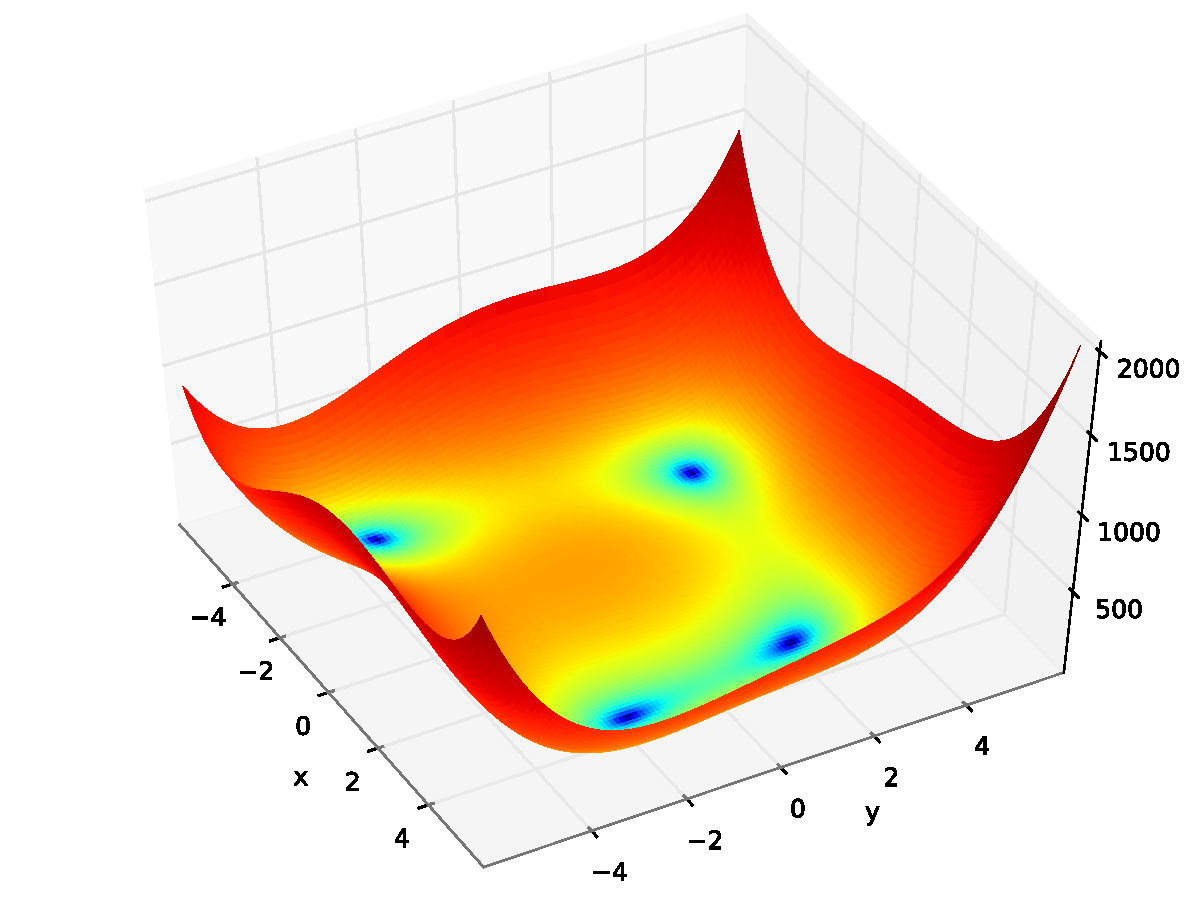
\includegraphics[width=\textwidth]{Chapter5/img/himmelblau.pdf}
    \caption{Himmelblau}
  \end{subfigure}
  \begin{subfigure}{0.24\textwidth}
    \centering\includegraphics[width=\textwidth]{Chapter5/img/rosenbrock.pdf}
    \caption{Rosenbrock}
  \end{subfigure}
  \begin{subfigure}{0.24\textwidth}
    \centering\includegraphics[width=\textwidth]{Chapter5/img/rastrigin.pdf}
    \caption{Rastrigin in 2D}
  \end{subfigure}
  \caption{Benchmark functions for testing black-box optimization algorithms.}
  \label{fig:benchmarks}
\end{figure}

\begin{figure}[ht]
  \centering
  \begin{subfigure}{0.49\textwidth}
    \centering\includegraphics[width=\textwidth]{Chapter5/img/branin_plot.pdf}
    \caption{Branin}
  \end{subfigure}
  \begin{subfigure}{0.49\textwidth}
    \centering\includegraphics[width=\textwidth]{Chapter5/img/himmelblau_plot.pdf}
    \caption{Himmelblau}
  \end{subfigure}
  \begin{subfigure}{0.49\textwidth}
    \centering\includegraphics[width=\textwidth]{Chapter5/img/rosenbrock_plot.pdf}
    \caption{Rosenbrock}
  \end{subfigure}
  \begin{subfigure}{0.49\textwidth}
    \centering\includegraphics[width=\textwidth]{Chapter5/img/rastrigin_plot.pdf}
    \caption{Rastrigin in 5D}
  \end{subfigure}
  \caption{Simple regret of \POO and \PCT run for different $\rho$ values.}
  \label{fig:results}
\end{figure}

In Figure~\ref{fig:results}, we plot the simple regret of the algorithms as a function of the number of evaluations. All the results are averaged over 5000 runs and we plot the simple regret after 500 function evaluations. Each instance of \HOO or \HCT would recommend a point picked uniformly at random among those evaluated so that we have the same recommendation strategy as \POO and \PCT.

The first observation is that \PCT does match the performance of some single \HCT instances as expected. We also notice that \PCT has comparable performance w.r.t.\,\POO in these plots, which justifies the choice of using \HCT as a subroutine for the \POO meta-algorithm.


% !TEX root = ../Chapter5.tex
\section{Discussion}\label{sec:gpo.discussion}

We studied \PCT, a new instantiation of \POO on top of \HCT. We proved that \HCT is a plausible subroutine for \POO by adapting the analysis of \HCT under a new assumption w.r.t.\,a fixed partitioning. We also proposed \GPO, a general framework for making any hierarchical bandit algorithm that only has a simple regret guarantee adaptive to unknown smoothness. However, whether it is possible to weaken the assumptions of \HOO in the same way as \HCT while keeping similar regret guarantees remains open.


% Manual newpage inserted to improve the layout of sample file - not
% needed in general before appendices/bibliography.

% \newpage
% \bibliographystyle{plainnat}
% \bibliography{Major,Minor}
% \newpage


	%%%%%%%%%%%%%%%%%%%%%%%%%%%%%%%%%%%%%%%%%%%%%%%%%%%%%%%%%%%%%%%%%%%%%%%%%%%%%%%%%%%%%%%%%%%%%
%%									Chapitre 6												%
%%%%%%%%%%%%%%%%%%%%%%%%%%%%%%%%%%%%%%%%%%%%%%%%%%%%%%%%%%%%%%%%%%%%%%%%%%%%%%%%%%%%%%%%%%%%%

\chapter{Bandits and Hyper-parameter Optimization}\label{chap:dttts}
	\citationChap{
		Et c'est là que jadis, à quinze ans révolus\\
		A l'âge où s'amuser tout seul ne suffit plus\\
		Je connus la prime amourette\\
		Auprès d'une sirène, une femme-poisson\\
		Je reçus de l'amour la première leçon\\
		Avalai la première arête
	}{Georges Brassens}
	\minitoc
	\newpage

%%%%%%%%%%%%%%%%%%%%%%%%%%%%%%%%%%%%%%%%%%%%%%%%%%%%%%%%%%%%%%%%%%%%%%%%%%%%%%%%%%%%%%%%%%%%%



% Début du chapitre
\addtocontents{toc}{\protect\setcounter{tocdepth}{1}}
\section{Introduction}\label{sec:dttts.intro}

Training a machine learning algorithm often requires to specify several parameters. For instance, for neural networks, it is the architecture of the network and also the parameters of the gradient algorithm used or the choice of regularization. These \emph{hyper-parameters} are difficult to learn through the standard training process and are often manually specified.
%\todo{some ref so this is not just blabla}

When it is not feasible to design algorithms with a few hyper-parameters, we opt for \emph{hyper-parameter optimization} (HPO).  HPO can be viewed as a \emph{black-box optimization} problem where the evaluation of the objective function is expensive as it is the accuracy of a learning algorithm for a given configuration of hyper-parameters. %Indeed, a typical function evaluation involves training the primary machine learning algorithm to completion on a large dataset, which often takes a considerable amount of time or resources. 
This vastly limits the number of evaluations that can be carried out, which calls for a design of efficient high-level algorithms that automate the tuning procedure.

Several naive but daily used HPO methods are  grid search and random search. More sophisticated methods address HPO as a \emph{sequential resource allocation problem}, by adaptively choosing the next hyper-parameter(s) to explore, based on the result obtained previously. For example, \emph{evolutionary optimization} follows a process inspired by the biological concept of \emph{evolution}, which repeatedly replaces the worst-performing hyper-parameter configurations from a randomly initialized population of solutions; see~\citet{loshchilov2016cmaes} for an example of using \texttt{CMA-ES} for hyper-parameter tuning. A major drawback of evolutionary optimization is its lack of theoretical understanding.

Bayesian optimization (BO) is another approach that leverages the sequential nature of the setting. BO depends on a prior belief for the target function, typically a Gaussian process. This prior distribution can be updated to a posterior given a sequence of observations. Several algorithms exploiting this posterior distribution to decide where to sample next have been given (see  \citealp{shahriari2016loop}, for a survey). \citet{snoek2012spearmint} and \citet{klein2017robo} provide Python packages called \Spearmint\ and \RoBO\ to perform hyper-parameter tuning with BO methods. Similar packages are available for \PyTorch\ (\BoTorch\footnote{\url{https://botorch.org/}}) and \TensorFlow\ (\flow\ by~\citealt{knudde2017gpflowopt}). Among BO algorithms, \TPE~\citep{bergstra2011tpe} and \SMAC~\citep{hutter2011smac} were specifically proposed for HPO. A shortcoming of BO is that most algorithms select where to sample next based on optimizing some \emph{acquisition function} computed from the posterior, e.g., the expected improvement~\citep{jones1998ei}. This auxiliary  task cannot be solved analytically but needs to be performed itself by optimization procedures as \LBFGS that make the process slow. %although this function is usually more regular than the target function.  

Bandits (see \citealp{lattimore2018} for a recent book) are a simple model for sequential resource allocation, and some bandit tools have already been explored for global optimization and HPO: First, in the field of Bayesian optimization, the \GPUCB algorithm \citep{srinivas2010gpucb} is a Gaussian process extension of the classical \UCB bandit algorithm \citep{auer2002ucb}. Later, \citet{hoffman2014bayesgap} proposed to use \emph{best-arm identification} (BAI) tools---still with a Bayesian flavor---for automated machine learning, where the goal is to smartly try hyper-parameters from a pre-specified \emph{finite} grid. 

However, in most cases, the number of hyper-parameter configurations to explore is infinite. In this paper, we investigate the use of bandit tools suited for an \emph{infinite} number of arms. There are two lines of work for tackling a very large or infinite number of configurations (arms). The first combines standard bandit tools with a hierarchical partitioning of the arm space and aims at exploiting the (possibly unknown) smoothness of the black-box function to optimize~\citep{bubeck2010x,grill2015poo,shang2019adaptive,bartlett2019simple}. To the best of our knowledge, these methods have never been investigated for HPO. The second line of work does not assume any smoothness: At each round, the learner may ask for a new arm from a \emph{reservoir distribution} $\nu_0$ (pick randomly a new hyper-parameter configuration) and add it to the current arm pool $\cA$, or re-sample one of the previous arms (evaluate configuration already included in $\cA$), in order to find an arm with a good mean reward (i.e., a hyper-parameter configuration with a good validation accuracy). The \emph{stochastic infinitely many-armed bandits} (SIAB) is studied by \citet{berry1997infinite,wang2008ucbv} for the rewards maximization problem while \citet{carpentier2015siri,aziz2018confidence} %\todo{add 2 other recent papers on this topic} 
study the simple regret problem, which is related to BAI. While most proposed algorithms consist of querying an \emph{adequate} number of arms from the reservoir before running a standard BAI algorithm, \cite{li2017hyperband} propose a more robust approach called \Hyperband that uses several such phases.

In this paper, we go even further and propose the first \emph{dynamic} algorithm for BAI in SIAB, that at each round, may either query a new arm from the reservoir or re-sample arms previously queried. Our algorithm leverages a Bayesian model and builds on the top-two Thompson sampling (\TTTS) algorithm by~\citet{russo2016ttts}. %We also introduce a variant of \Hyperband where the \texttt{SHA} sub-routine \citep{karnin2013sha} is replaced by \TTTS. 
An extensive numerical study is presented to show the competitiveness of our algorithm with respect to state-of-the-art HPO methods.
%\todo{cut this in space needed}
%\paragraph{Outline} We first introduce a general framework for hyper-parameter optimization in Section~\ref{sec:framework}. In Section~\ref{sec:bai}, we explain how infinitely-many armed bandit algorithms can be used for HPO, before presenting our two new algorithms in Section~\ref{sec:algo}. Finally, we provide experimental results in Section~\ref{sec:result}. % before concluding.


\section{A Brief Survey of Automated Machine Learning}\label{sec:dttts.survey}


\section{Hyper-Parameter Optimization Framework}\label{sec:dttts.framework}

In this paper, we view \gls{hpo} as a particular \gls{go} setting, for which the target function $f$ is a mapping from a hyper-parameter configuration to some measure of failure for the machine learning algorithm trained with these hyper-parameters. Formally, we aim at solving an optimization problem of the form $f^\star = \min \{f(\blambda):\blambda\in\Omega\}$, where $\blambda$ denotes a configuration of hyper-parameters chosen from a configuration space $\Omega$. A hyper-parameter optimizer is a sequential procedure, that at each round $t$, selects a configuration~$\blambda_t$ to evaluate using some sampling rule, after which a (costly and \emph{noisy}) evaluation of $f(\blambda_t)$ is observed. Besides, a hyper-parameter configuration $\hat{\blambda}^\star$ is recommended as a guess for a close-to-optimal configuration at the end. The hope is that $f(\hat{\blambda}^\star)$ is not far from $f^\star$.

We restrict our presentation to hyper-parameter tuning for supervised learning algorithms. Given a training dataset $\cD_{\texttt{train}}$ containing $n$ labeled examples in $\cX \times \cY$ and a choice of hyper-parameter configuration $\blambda$, a supervised learning algorithm (neural network, \SVM, gradient boosting, \dots) produces a predictor $\hat{g}_{\bm\lambda}^{\,(n)}\!:\cX \rightarrow \cY$. Note that there can be some randomness in the training process (e.g., if stochastic gradient descent is used) so that $\hat{g}_{\blambda}^{\,(n)}$ may still be random for a given training set and hyper-parameters. The goal is to build a predictor that generalizes well. If we had access to the distribution $\bP$ that generated the data (i.e., assuming that data points in $\cD_{\texttt{train}}$ are i.i.d. from $\bP$), this generalization power would be measured by the risk $f(\bm\lambda) \triangleq \mathbb{E}\left[\ell\left(\bm Y,\hat g_{\blambda}^{\,(n)}(\bm X)\right) \right]$, where $\ell$ is some loss function measuring the distance between two predictions and the expectation is taken on $(\bm X , \bm Y) \sim \bP$ and the possible randomness in the training process. 


% Given a set of hyper-parameters $\blambda$, the objective of a (supervised) learning process is to train a model $g_{\blambda}:\cX\lra\cY$ that minimizes the total empirical loss (could be regularized) over a training set $\cD_{\texttt{train}} = \{(\bx_i,\by_i)_{i=1, \ldots, |\cD_{\texttt{train}}|}\}$ where $(\bx_i,\by_i)\in\cX\times\cY$ are pairs of input and output,
% \[
% 	\cL_{\texttt{train}}(\blambda) \eqdef \sum_{i=1}^{|\cD_{\texttt{train}}|} \ell_1(g_{\blambda}(\bx_i),\by_i).
% \]
% Here the loss function $\ell_1$ should be neatly chosen for a specific task.
% 
% In the context of hyper-parameter tuning, our objective is then to minimize the following black-box function
% \[
%     f(\blambda) \eqdef \EE{\mathbb{P}_{\bx,\by\sim \cD_{\texttt{valid}}}\left[\by\neq\hat{g}_{\blambda}(\bx)\right]},
% \]
% where the randomness of the expectation comes eventually from the training set that we are using. 

In practice, however, the explicit evaluation of $f$ is impossible, but there are several methods for \emph{noisy evaluations}. We can either compute the validation error of $\hat g_{\blambda}^{\,(n)}$ on a held-out validation set,  $1/|\cD_{\texttt{valid}}| \sum_{i=1}^{|\cD_{\texttt{valid}}|} \ell(\hat{g}^{\,(n)}_{\blambda}(\bx_i),\by_i)$, or a cross validation error over the training set as an approximation of the  objective. %We specify this loss function for real hyper-parameter optimization tasks in Section~\ref{sec:result}.


\section{Active \TTTS{} for Hyper-Parameter Optimization}\label{sec:dttts.algorithm}

In this section, we introduce a new algorithm for \gls{bai} in an infinite bandit model, that is an adaptation of \gls{ttts}{} (see Chapter~\ref{CHAP:T3C}). Unlike \SHA{} that requires the knowledge of the total budget to operate, \gls{ttts}{} is particularly appealing as it does not need to have it. Remember that such algorithms are referred to as \emph{anytime}. Besides, it is known to be optimal in a Bayesian (asymptotic) sense (see Chapter~\ref{CHAP:T3C}).

Recall that as a Bayesian algorithm, \gls{ttts} uses a prior distribution $\Pi_0$ over the vector of means of the $K$ arms, $\bmu \triangleq (\mu_1,\cdots,\mu_K)$, which can be updated to a posterior distribution $\Pi_n$ after $n$ observations. 

We consider Bernoulli bandit model in the rest of this chapter. Under Bernoulli bandit model, arm $i$ produces a reward $r_{n,i}=1$ with probability $\mu_i$, and $r_{n,i}=0$ with probability $1-\mu_i$ when sampled at round $n$. Given independent uniform prior for the mean of each arm, the posterior distribution on $\bmu$ is a product of $K$ Beta distributions: $\Pi_n = \bigotimes_{i=1}^{K} \texttt{Beta}(1+S_{n,i},N_{n,i}-S_{n,i}+1)$, where $N_{n,i}$ is the number of selections of arm $i$ until round $n$ and $S_{n,i}$ is the sum of rewards obtained from that arm. 
%At each round $n$, \gls{ttts} chooses one arm from the following two candidates to evaluate: (1) it first samples a parameter ${\bm\theta}$ from $\Pi_{t-1}$, and the first candidate is defined as $I_n^{\,(1)} \eqdef \argmax_{i\in\cX} {\theta}_i$, (2) it repeatedly samples new ${\bm\theta}'$ until $I_n^{\,(2)} \eqdef \argmax_{i\in\cX} \theta_i'$ is different from $I_n^{\,(1)}$. \gls{ttts} depends on a parameter $\beta \in (0,1)$. In particular, the algorithm selects $I_n = I_n^{\,(1)}$ with probability $\beta$ and $I_n = I_n^{\,(2)}$ with probability $1-\beta$.

\paragraph{Why variants of \TTTS{}?}
We further motivate experimentally in this section why we choose to build new algorithms upon \gls{ttts}.

We compare \gls{ttts} against some fixed-budget \gls{bai} algorithms as benchmark, including uniform allocation~\citep{bubeck2009pure}, \UCBE{} and \SR{}~\citep{audibert2010budget}, \UGapE~\citep{gabillon2012ugape}, \SHA{}, \TS{} with a MPA strategy of decision (see Section~\ref{sec:mab.bai.decision}), and one anytime algorithm \ATLUCB{}~\citep{jun2016atlucb}.

We use 8 problem instances proposed by~\cite{audibert2010budget}, all settings consider Bernoulli bandits, and we compare their trending \gls{simple regret} (see Definition~\ref{def:mab.simple_regret}) averaged on 1000 trials. The results are shown in Fig.~\ref{fig:bai}.

Note that contrary to Chapter~\ref{CHAP:T3C}, we are interested in the fixed-budget setting in this chapter, hence the present experimental study with simple regret as performance measure.

\begin{itemize}
	\item Setting 1: $\mathbf{\mu_1}=0.5, \mathbf{\mu_{2:20}}=0.4, \operatorname{budget}=2000$
	\item Setting 2: $\mathbf{\mu_1}=0.5, \mathbf{\mu_{2:6}}=0.42, \mathbf{\mu_{7:20}}=0.38, \operatorname{budget}=2000$
	\item Setting 3: $\mathbf{\mu}=[0.5, 0.3631, 0.449347, 0.48125839], \operatorname{budget}=2000$
	\item Setting 4: $\mathbf{\mu}=[0.5, 0.42, 0.4, 0.4, 0.35, 0.35], \operatorname{budget}=600$
	\item Setting 5: $\mathbf{\mu_1}=0.5, \mathbf{\mu_i}=\mathbf{\mu_1}-0.025i, \forall i\in\{2\ldots15\}, \operatorname{budget}=4000$
	\item Setting 6: $\mathbf{\mu_1}=0.5, \mathbf{\mu_2}=0.48, \mathbf{\mu_{3:20}}=0.37, \operatorname{budget}=6000$
	\item Setting 7: $\mathbf{\mu_1}=0.5, \mathbf{\mu_{2:6}}=0.45, \mathbf{\mu_{7:20}}=0.43, \mathbf{\mu_{7:20}}=0.38, \operatorname{budget}=6000$
	\item Setting 8: $\mathbf{\mu_1}=0.5, \mathbf{\mu_{2:6}}=0.45, \mathbf{\mu_{7:20}}=0.43, \mathbf{\mu_{7:20}}=0.38, \operatorname{budget}=12000$
\end{itemize}

\begin{figure}[ht]
  \centering
  \begin{subfigure}[t]{0.25\textwidth}
    \centering\includegraphics[width=\textwidth]{Chapter6/img/bai/setting1.png}
    \caption{Problem 1}
  \end{subfigure}%
  \begin{subfigure}[t]{0.25\textwidth}
    \centering\includegraphics[width=\textwidth]{Chapter6/img/bai/setting2.png}
    \caption{Problem 2}
  \end{subfigure}
  \begin{subfigure}[t]{0.25\textwidth}
    \centering\includegraphics[width=\textwidth]{Chapter6/img/bai/setting3.png}
    \caption{Problem 3}
  \end{subfigure}%
  \begin{subfigure}[t]{0.25\textwidth}
    \centering\includegraphics[width=\textwidth]{Chapter6/img/bai/setting4.png}
    \caption{Problem 4}
  \end{subfigure}
  \begin{subfigure}[t]{0.25\textwidth}
    \centering\includegraphics[width=\textwidth]{Chapter6/img/bai/setting5.png}
    \caption{Problem 5}
  \end{subfigure}
  \begin{subfigure}[t]{0.25\textwidth}
    \centering\includegraphics[width=\textwidth]{Chapter6/img/bai/setting6.png}
    \caption{Problem 6}
  \end{subfigure}
  \begin{subfigure}[t]{0.25\textwidth}
    \centering\includegraphics[width=\textwidth]{Chapter6/img/bai/setting7.png}
    \caption{Problem 7}
  \end{subfigure}
  \begin{subfigure}[t]{0.25\textwidth}
    \centering\includegraphics[width=\textwidth]{Chapter6/img/bai/setting8.png}
    \caption{Problem 8}
  \end{subfigure}
  \caption{Simple regret as a function of allocation budget for various BAI algorithms.}
  \label{fig:bai}
\end{figure}

In these experiments, \gls{ttts} are always beating or at least performing as well as its competitors. It thus seems to be a good candidate to be further investigated.

Note that \gls{ttts} can also be used for bandit settings in which the rewards are bounded in $[0,1]$ by using a binarization trick first proposed by~\cite{agrawal2012analysis}: When a reward $r_{n,i} \in [0,1]$ is observed, the algorithm is updated with a fake reward  
\[
    r'_{n,i} \sim \texttt{Bern}(r_{n,i}) \in \{0,1\}\,.
\]
\gls{ttts} can thus be used for \gls{bai} for a \emph{finite} number of arms that with rewards in $[0,1]$. We now present a simple way of extending \gls{ttts}{} to deal with an infinite number of arms, namely \gls{dttts}.

\paragraph{Dynamic \TTTS{}.}

%The rationale behind \DTTTS is the following. 

In an infinite bandit algorithm, at each round, we either query a new arm from the reservoir \emph{and sample it}, or re-sample a previous arm. In a Bayesian setting, we can also imagine that at each round, an arm is queried from the reservoir and added with a \textit{uniform prior} to the list of queried arms, \emph{regardless of whether it is sampled or not}. Then, at round $t$, \DTTTS consists in running \gls{ttts} on these $t$ arms, out of which several are endowed with a uniform prior and have never been sampled. 

Leveraging the fact the the maximum of $k$ uniform distribution has a \texttt{Beta}($k,1$) distribution and that \gls{ttts} only depends on the maxima of posterior samples, we give the following equivalent implementation for \DTTTS (Algorithm~\ref{alg:dttts}). Letting $\cL_n$ be the list of arms that have been queried  from the reservoir and sampled \textit{at least once} before round $t$, at round $t$ we run \gls{ttts} on the set $\cX_n \triangleq \cL_n \cup \{\mu_0\}$ where $\mu_0$ is a pseudo-arm with posterior distribution \texttt{Beta}($n-k_n, 1$), where $k_n\triangleq|\cL_n|$.  

\begin{algorithm}[ht]
\centering
\caption{Sampling rule of \DTTTS{}}
\label{alg:dttts}
\begin{algorithmic}[1] %[1] enables line numbers
    \State {\bfseries Input: } $\beta$; $B$ (total budget); $\nu_0$
    \State {\bfseries Initialization: } $\mu_1 \sim \nu_0$; $t \gets 0$; $\cX \gets \{\mu_0,\mu_1\}$; $m\gets1$; $S_0, N_0 \gets 0$; $S_1 \sim \texttt{Bern}(\mu_1)$, $N_1 \gets 1$\
    
    \While{$n < B$}
	    \State $\forall i=0,\dots,m$, $\theta_i \sim \texttt{Beta}(S_i+1,N_i-S_i+1)$; $U \sim \cU([0,1])$
	    \State $I^{\,(1)} \gets \argmax_{i=0,\dots,m} \theta_i$
	    \If{$U > \beta$}
	        \While{$I^{\,(2)} = I^{\,(1)}$} 
	            \State $\forall i=0,\dots,m, \theta_i' \sim \texttt{Beta}(S_i+1,N_i-S_i+1)$
	            \State $I^{\,(2)} \leftarrow \argmax_{i=0,\dots,m}\theta_i'$ 
	        \EndWhile
	        \State $I^{\,(1)} \gets I^{\,(2)}$
	    \EndIf
	    \If{$I^{\,(1)} \neq 0$}
	        \State $Y \leftarrow$ \text{Evaluate arm} $I^{\,(1)}$; $X \sim \texttt{Bern}(Y)$ 
	        \State $S_{I^{\,(1)}} \gets S_{I^{\,(1)}} + X$; $N_{I^{\,(1)}} \gets N_{I^{\,(1)}} + 1$; $S_0 \gets S_0 + 1$
	    \Else
            \State $\mu_{m+1}\sim \nu_0$; $\cX \gets \cX \cup \{\mu_{m+1}\}$; 
            \State $Y \leftarrow$ \text{Evaluate arm} $m+1$; $X \sim \texttt{Bern}(Y)$
           	\State $S_{m+1} \gets X$; $N_{m+1}
           	\gets 1$; $m \gets m + 1$
 	   \EndIf
  	   \State $t\gets t+1$
    \EndWhile
\end{algorithmic}
\end{algorithm}

It remains to decide how to recommend the arm as our best guess. It is obviously not a good idea to output the arm with the best empirical means since some lately sampled arms may have very high empirical mean with no confidence. In this chapter, we choose the most natural recommendation strategy for Bayesian algorithms that outputs the arm with the largest optimal action probability (see Section~\ref{sec:t3c.algorithm}). Let $\Theta_i$ be the subset of the set $\Theta$ of possible mean vectors such that arm $i$ is optimal, $\Theta_i \eqdef \big\{ \btheta\in\Theta \,|\, \theta_i > \max_{j\neq i}\theta_j \big\}$, the posterior probability that arm $i$ is optimal after round $t$ is defined as $\Pi_{n}(\Theta_i)$. At any time $n$, we therefore recommend  arm 
\[
    J_n \eqdef \argmax_{i\in\cX} \Pi_{n}(\Theta_i)\,.
\]

\paragraph{Hyper-\TTTS{}.}

We present here also another simple way of extending \gls{ttts} to deal with an infinite number of arms, namely \texttt{Hyper}-\gls{ttts} or \HTTTS, a variant of \Hyperband in which \texttt{SHA} is replaced by \gls{ttts}. This algorithm, whose sampling rule is formally stated as Algorithm~\ref{alg:httts}, runs $s_{\max}$ batches of \gls{ttts} with different number of arms $n$ and each batch with a same budget $T=\ceil{B/s_{\max}}$ with $B$ the total budget. The number of arms within each bracket is decreasing with an exponential rate of~$\gamma$. One inconvenience of this algorithm is that $s_{\max}$ and~$\gamma$ still need to be tuned (in practice, we use the same tuning as the one of \Hyperband). \DTTTS is thus proposed to circumvent this issue. 

\begin{algorithm}[ht]
\centering
\caption{Sampling rule of \HTTTS{}}
\label{alg:httts}
\begin{algorithmic}[1] %[1] enables line numbers
    \State {\bfseries Input: } $\beta$; $\gamma$; $B$; $s_{\operatorname{max}}$; $\nu_0$
    \State {\bfseries Initialization: } $T=\floor{B/s_{\operatorname{max}}}$

    \For{$s \leftarrow s_{\operatorname{max}}$ to $0$}
    	\State $K = \ceil{\frac{s_{\operatorname{max}}+1}{s+1}\gamma^s}$
    	\State $\cX \leftarrow \{i=1,\ldots,K: \mu_i\sim\nu_0\}$; $t=0$
    	\While{$t < T$}
    		\State \text{Sample} $\btheta \sim \Pi_n$
            \State $I^{(1)} \leftarrow \argmax_{i\in\cX}\theta_i$
    	    \State \text{Sample} $b \sim \operatorname{Bernoulli}(\beta)$
    	    \If{$b = 1$}
    	        \State $Y \leftarrow$ \text{Evaluate arm} $I^{(1)}$
    	    \Else
    	        \While{$I^{(2)} = I^{(1)}$} 
    	            \State $\forall i\in\cX, \theta_i' \sim \texttt{Beta}(S_i+1,N_i-S_i+1)$
    	            \State $I^{(2)} \leftarrow \argmax_{i \in \cX}\theta_i'$ 
    	        \EndWhile
    	        \State $I^{(1)} \gets I^{(2)}$
    		    \State $Y \leftarrow$ \text{Evaluate arm} $I^{(1)}$
    	    \EndIf
    	    \State $X \sim \texttt{Bernoulli}(Y)$ 
    	    \State $S_{I^{(1)}} \gets S_{I^{(1)}} + X$; $N_{I^{(1)}} \gets N_{I^{(1)}} + 1$
    		\State $t = t+1$
        \EndWhile
    \EndFor
\end{algorithmic}
\end{algorithm}



\section{Experiments}\label{sec:dttts.experiments}

We benchmark our bandit-based strategy against different types of HPO algorithms, namely, \TPE, random search, \Hyperband and a simple Thompson sampling variant of \Hyperband (called \HTTTS described in Appendix~\ref{app:dttts.httts}), for the tuning of classifiers (\SVM and \MLP) on 4 different classification tasks: \textit{wine}, \textit{breast cancer}, and \textit{adult} datasets from \UCI machine learning repository \citep{dua2017}; and the \MNIST dataset~\citep{lecun1998gradient}.

For all the methods, a noisy evaluation of the black-box function $f$ (see the terminology introduced in Section~\ref{sec:dttts.framework}) for a hyper-parameter configuration $\bm\lambda$ consists in performing a shuffled 3-fold cross-validation on $\cD_{\texttt{train}}$. More precisely, given a random partitioning $\cup_{j=1}^3\cD_{\texttt{valid}}^j$ of $\cD_{\text{train}},$ where the folds are of equal size, we train a classifier $\hat{g}^{\,(j)}_{\bm\lambda}$ on $\cD_{\texttt{train}} \backslash \cD_{\texttt{valid}}^j$ for each fold $j$ and compute the average validation error defined as $e \triangleq 1/|\cD_{\texttt{train}}|\sum_{j=1}^{3} \sum_{i \in \cD_{\text{valid}}^j} \mathbbm{1}\{\hat{g}^{\,(j)}_{\blambda}(\bx_i)\neq\by_i\},$ which we report as a noisy estimate of the risk $f(\bm\lambda) \triangleq \bP(\hat{g}^{\,(n)}_{\bm\lambda}(\bm X) \neq \bm Y)$.

Observe that both the noisy evaluation and the value of $f$ belong to $[0,1]$. Therefore we can introduce an \textit{arm} with rewards in $[0,1]$ for each hyper-parameter~$\bm\lambda$. Sampling  arm~$\bm\lambda$ produces reward $r \triangleq 1-e \in [0,1]$ with a different random partitioning and random seed for training for each selection. Arm~$\lambda$ is assumed to have mean of $1-f(\bm\lambda)$. In an infinite arm setting, querying a new arm from the reservoir corresponds to selecting a new hyper-parameter at random from the search space. With these two notions (\textit{arm sampling} and \textit{reservoir querying}), our algorithm for infinite BAI applies to HPO.  

For the experiments, we adapt the recommendation rule of \DTTTS to the HPO applications considered and always recommend the hyper-parameter configuration that has produced the smallest cross-validation error so far (which is also the recommendation rule used by other approaches, e.g., \Hyperband). For all methods, we report the cross-validation error for the recommended hyper-parameter configuration, as a function of time. We stress again that, unlike in standard bandits, where we could use the simple regret as a performance metric, we do not have access to the ground truth generalization error in real classification tasks. Therefore, we only report a proxy of the true error rate that we are interested in.

\paragraph{Results} We first benchmark\footnote{Code at \url{http://researchers.lille.inria.fr/~valko/hp/publications/shang2019simple.code.zip}} our methods on a few simple \UCI datasets using \SVM from \Scikit as the classifier. We  optimize over two hyper-parameters: the \emph{penalty parameter} $C$ and the \emph{kernel coefficient}~$\gamma$\footnote{$\gamma$ is the parameter of the RBF kernel defined as $\exp(-\gamma||\bx-\bx'||^2)$}
for an RBF kernel, for which the pre-defined search bounds are both $\left[10^{-5}, 10^{5} \right]$.

%\begin{table}[ht]
%\centering
%\begin{tabular}{@{}l|lll@{}}
%\toprule
%\textbf{Classifier} & \textbf{Hyper-parameter}             & \textbf{Type}  & %\textbf{Bounds}                          \\ \midrule
%\Ada & \texttt{learning\_rate}      & $\mathbb{R}^+$ & $\left[10^{-5}, 10^{-1}\right]$                         \\
%& \texttt{n\_estimators}       & Integer        & $\left\lbrace 5,\dots, 200 \right\rbrace$ \\ \midrule
%& \texttt{learning\_rate}      & $\mathbb{R}^+$ & $\left[10^{-5}, 10^{-2}\right]$                         \\
%\GBM & \texttt{n\_estimators}       & Integer        & $\left\lbrace 10,\dots, 100 \right\rbrace$ \\
%& \texttt{max\_depth}          & Integer        & $\left\lbrace 2, \dots, 100 \right\rbrace$ \\
%& \texttt{min\_samples\_split}  & Integer        & $\left\lbrace 2, \dots, 100 \right\rbrace$ \\ \midrule
%\KNN & $k$                & Integer       & $\left\lbrace 10, \dots,50 \right\rbrace$ \\ \midrule
%\SVM & $C$                & $\mathbb{R}^+$ & $\left[ 10^{-5}, 10^{5} \right]$ \\
%& $\gamma$           & $\mathbb{R}^+$ & $\left[10^{-5}, 10^{5} \right]$  \\ \bottomrule
%\end{tabular}
%\caption{Hyper-parameters to be optimized for \UCI experiments.}
%\label{hyper_uci}
%\end{table}

%\todo{For the figures, can we have less white space and bigger figures? (probably some margin, or use crop)}
\begin{figure}[ht]
	\centering
	\begin{subfigure}[t]{0.33\textwidth}
    		\includegraphics[width=\textwidth]{Chapter6/img/uci/wine.pdf}
    		\caption{wine}
    		\label{fig:wine}
	\end{subfigure}
	\begin{subfigure}[t]{0.33\textwidth}
    		\includegraphics[width=\textwidth]{Chapter6/img/uci/breast_cancer.pdf}
    		\caption{breast cancer}
    		\label{fig:breast_cancer}
	\end{subfigure}
	\begin{subfigure}[t]{0.33\textwidth}
    		\includegraphics[width=\textwidth]{Chapter6/img/uci/adult.pdf}
    		\caption{adult}
    		\label{fig:adult}
	\end{subfigure}
	\begin{subfigure}[t]{0.33\textwidth}
    		\includegraphics[width=\textwidth]{Chapter6/img/mnist/mnist.pdf}
    		\caption{\MNIST}
    		\label{fig:mnist}
	\end{subfigure}
	\caption{Mean cross-validation error of different HPO algorithms with (a) \SVM run on the \UCI wine dataset, (b) \SVM run on the \UCI breast cancer dataset, (c) \SVM run on the \UCI adult dataset and (d) \MLP run on the \MNIST dataset.}
\end{figure}

Fig.\,\ref{fig:wine} shows the mean cross-validation error of \SVM run on the \UCI wine dataset over 24 pulls\footnote{The number of pulls here and later is chosen exactly as in the work of \citet{li2017hyperband}} averaged on 100 runs. The task is to predict the quality score  of wine (between 0 and 10) given 11 attributes. Recall that one iteration corresponds to one arm pull. In this experiment, \DTTTS improves over other benchmark algorithms. Fig.\,\ref{fig:breast_cancer} is the same experiment run on the \UCI breast cancer dataset over 81 pulls. The task is to predict whether a patient has breast cancer based on 32 attributes. We repeat the experiment 100 times. This time, \DTTTS is slightly worse than \Hyperband at the beginning, but improves later. Finally, we optimize \SVM on a relatively more complicated \UCI adult dataset over 162 pulls, for which the result is shown in Fig.\,\ref{fig:adult}. The task is to tell whether the income of an individual is higher than 50k or not given 14 attributes. This experiment is also averaged over 100 runs. \DTTTS is better than other algorithms at the beginning, but is outperformed by \TPE towards the end. We see that, although not always the best, \DTTTS shows a consistent, robust, and quite competitive performance in the 3 tasks. 

We now carry out the classic \MNIST digits classification task using multi-layer perceptron (\MLP). We choose to optimize over three hyper-parameters: the \emph{size of hidden layer} (an integer between 5 and 50), the \emph{$\ell_2$ penalty parameter} $\alpha$ (between 0 and 0.9) and the \emph{initial learning rate} (bounded in $\left[10^{-5}, 10^{-1} \right]$). Fig.\,\ref{fig:mnist} shows the result of \MLP run on \MNIST over 108 pulls, this time averaged over 20 runs. \DTTTS is slightly worse than \Hyperband and \HTTTS in the very beginning, but is performing well afterward. %We notice that, although always showing bad performance in the \UCI tasks, \HTTTS shows a good behavior for the \MNIST task.

%\begin{table}[ht]
%\centering
%\begin{tabular}{@{}l|lll@{}}
%\toprule
%\textbf{Classifier} & \textbf{Hyper-parameter}             & \textbf{Type}  & \textbf{Bounds}                          \\ \midrule
%\MLP & \texttt{hidden\_layer\_size} & Integer          & $\left[5, 50\right]$  \\
%& \texttt{alpha}               & $\mathbb{R}^{+}$ & $\left[0, 0.9\right]$ \\ 
%& \texttt{learning\_rate\_init} & $\mathbb{R}^{+}$ & $\left[ 10^{-5}, 10^{-1} \right]$ \\ \bottomrule
%\end{tabular}
%\caption{Hyper-parameters to be optimized for \MNIST experiments.}
%\label{hyper_mnist}
%\end{table}

% \begin{figure}[ht]
%     \centering\includegraphics[width=0.6\textwidth]{Chapter6/img/mnist/mnist.pdf}
%     \caption{\MNIST dataset}
%     \label{fig:mnist}
% \end{figure}


\section{Discussion}\label{sec:dttts.discussion}

We presented a way to use Thompson sampling for BAI for infinitely many-armed bandits and explained how to use it for HPO. We introduced the \textit{first fully dynamic algorithm} for this setting and showed through an empirical study that it is a promising approach for HPO. In the future, we plan to provide experiments on more datasets and establish theoretical guarantees to support the good performance of \DTTTS, with the hope to provide a finite-time upper bound on its probability of error. We also plan to investigate variants of this algorithm for the non-stochastic bandits for which \Hyperband can be used, which would allow spending more time on the more promising algorithms.


\begin{subappendices}
\addtocontents{toc}{\protect\setcounter{tocdepth}{0}}
\section{Hyper \TTTS}\label{app:dttts.httts}

We present here another way of extending \TTTS to deal with an infinite number of arms, namely \texttt{Hyper}-\TTTS or \HTTTS, a variant of \Hyperband in which \texttt{SHA} is replaced by \TTTS. This algorithm, whose sampling rule is formally stated as Algorithm~\ref{alg:httts}, runs $s_{\max}$ batches of \TTTS with different number of arms $n$ and each batch with a same budget $T=\ceil{B/s_{\max}}$ with $B$ the total budget. The number of arms within each bracket is decreasing with an exponential rate of~$\gamma$. One inconvenience of this algorithm is that $s_{\max}$ and~$\gamma$ still need to be tuned (in practice, we use the same tuning as the one of \Hyperband). \DTTTS is thus proposed to circumvent this issue. 

\begin{algorithm}[tb]
\centering
\caption{Hyper \TTTS (\HTTTS)}
\label{alg:httts}
\begin{algorithmic}[1] %[1] enables line numbers
    \State {\bfseries Input: } $\beta$; $\gamma$; $B$; $s_{\operatorname{max}}$; $\nu_0$
    \State {\bfseries Initialization: } $T=\floor{B/s_{\operatorname{max}}}$

    \For{$s \leftarrow s_{\operatorname{max}}$ to $0$}
    	\State $K = \ceil{\frac{s_{\operatorname{max}}+1}{s+1}\gamma^s}$
    	\State $\cA \leftarrow \{i=1,\ldots,K: \mu_i\sim\nu_0\}$; $t=0$
    	\While{$t < T$}
    		\State \texttt{sample} $\btheta \sim \Pi_t$
            \State $I^{(1)} \leftarrow \argmax_{i\in\cA}\theta_i$
    	    \State \texttt{sample} $b \sim \operatorname{Bernoulli}(\beta)$
    	    \If{$b = 1$}
    	        \State $Y \leftarrow$ \texttt{evaluate arm} $I^{(1)}$
    	    \Else
    	        \While{$I^{(2)}\neq I^{(1)}$} 
    	            \State $\forall i\in\cA, \theta_i' \sim \texttt{Beta}(S_i+1,N_i-S_i+1)$
    	            \State $I^{(2)} \leftarrow \argmax_{i \in \cA}\theta_i'$ 
    	        \EndWhile
    	        \State $I^{(1)} \gets I^{(2)}$
    		    \State $Y \leftarrow$ \texttt{evaluate arm} $I^{(1)}$
    	    \EndIf
    	    \State $X \sim \texttt{Bernoulli}(Y)$ 
    	    \State $S_{I^{(1)}} \gets S_{I^{(1)}} + X$; $N_{I^{(1)}} \gets N_{I^{(1)}} + 1$
    		\State $t = t+1$
        \EndWhile
    \EndFor
\end{algorithmic}
\end{algorithm}


\section{Some Synthetic Results}\label{app:dttts.experiments}
In this part, we give some synthetic experimental results comparing \DTTTS to \Hyperband and to \texttt{SHA}, a state-of-the-art algorithm for finite BAI that can be adapted to the infinite setting. In those experiments, the arms are Bernoulli distributed and the reservoir distribution $\nu_0$ is fixed to some $\text{Beta}(a,b)$ distribution. 

Infinite Sequential Halving (\ISHA) consists in running \texttt{SHA} on a fixed number of arms drawn from the reservoir. Observe that for a total budget $B$, there exists a maximum number of arms $K^\star$ that can be processed by \texttt{SHA}, which satisfies $B = \ceil{K^\star\log_2(K^\star)}$. Following~\cite{aziz2018infinite}, we run \ISHA with $K^\star$ arms drawn from the reservoir. % seems to be empirically performing better than \Hyperband.

We report in Fig.\,\ref{fig:dttts} the simple regret as a function of time for different algorithms and four Beta reservoir distributions. $\HTTTS$ and $\DTTTS$ are run with $\beta=1/2$ which is known to be a robust choice \citep{russo2016ttts}. Each point represents the expected simple regret $\mathbb{E}[1 - \mu_{I_n^*}]$ estimated over 1000 replications for an algorithm run with budget $n$. \DTTTS is very competitive on 3 reservoirs and \HTTTS is sometimes better, sometimes worse than \Hyperband. We also tried the \SiRI algorithm \citep{carpentier2015siri} (with $b$ as the tail parameter when $\nu_0=$Beta$(a,b)$) but obtained worse performance and therefore do not report the results.

\begin{figure}[ht]
  \centering
  \begin{subfigure}[t]{0.2\textwidth}
    \centering\includegraphics[width=\textwidth]{Chapter5/img/infinite/beta_1_1.pdf}
    \caption{Beta(1,1)}
  \end{subfigure}%
\begin{subfigure}[t]{0.2\textwidth}
    \centering\includegraphics[width=\textwidth]{Chapter5/img/infinite/beta_3_1.pdf}
    \caption{Beta(3,1)}
  \end{subfigure}
  \begin{subfigure}[t]{0.2\textwidth}
    \centering\includegraphics[width=\textwidth]{Chapter5/img/infinite/beta_1_3.pdf}
    \caption{Beta(1,3)}
  \end{subfigure}%
  \begin{subfigure}[t]{0.2\textwidth}
    \centering\includegraphics[width=\textwidth]{Chapter5/img/infinite/beta_-5_-5.pdf}
    \caption{Beta(0.5,0.5)}
  \end{subfigure}
  \caption{Simple regret of \DTTTS (against \Hyperband) as a function of the number of arms evaluations for different Beta reservoir.}
  \label{fig:dttts}
\end{figure}

Note that in the implementation of \Hyperband for this \emph{stochastic} infinite bandit setting, the elimination phase of the underlying \texttt{SHA} algorithm is carried out according to the averaged loss of previous samples (as samples from an arm are i.i.d. in this setting and not a converging sequence). In the next section, we apply our algorithm to some real hyper-parameter optimization tasks. 

%\begin{figure}[ht]
%  \centering
%  \begin{subfigure}[t]{0.2\textwidth}
%    \centering\includegraphics[width=\textwidth]{Chapter5/img/infinite/beta_1_1_64.pdf}
%    \caption{Beta(1,1)}
%  \end{subfigure}%
%  \begin{subfigure}[t]{0.2\textwidth}
%    \centering\includegraphics[width=\textwidth]{Chapter5/img/infinite/beta_3_1_64.pdf}
%    \caption{Beta(3,1)}
%  \end{subfigure}
%  \begin{subfigure}[t]{0.2\textwidth}
%    \centering\includegraphics[width=\textwidth]{Chapter5/img/infinite/beta_1_3_64.pdf}
%    \caption{Beta(1,3)}
%  \end{subfigure}%
%  \begin{subfigure}[t]{0.2\textwidth}
%    \centering\includegraphics[width=\textwidth]{Chapter5/img/infinite/beta_-5_-5_64.pdf}
%    \caption{Beta(0.5,0.5)}
%  \end{subfigure}
%  %\begin{subfigure}[t]{0.2\textwidth}
%  %  \centering\includegraphics[width=\textwidth]{Chapter5/img/infinite/beta_2_5_64.pdf}
%  %  \caption{Beta(2,5)}
%  %\end{subfigure}
%  %\begin{subfigure}[t]{0.2\textwidth}
%  %  \centering\includegraphics[width=\textwidth]{Chapter5/img/infinite/beta_5_2_64.pdf}
%  %  \caption{Beta(5,2)}
%  %\end{subfigure}
%  %\begin{subfigure}[t]{0.2\textwidth}
%  %  \centering\includegraphics[width=\textwidth]{Chapter5/img/infinite/beta_2_2_64.pdf}
%  %  \caption{Beta(2,2)}
%  %\end{subfigure}
%  %\begin{subfigure}[t]{0.2\textwidth}
%  %  \centering\includegraphics[width=\textwidth]{Chapter5/img/infinite/beta_-3_-7_64.pdf}
%  %  \caption{Beta(0.3,0.7)}
%  %\end{subfigure}
%  \caption{}
%  \label{fig:dttts1}
%\end{figure}


\section{Illustration of Effectively Sampled Arms by \texorpdfstring{\DTTTS}{}}\label{app:dttts.arms}

One drawback of the current \DTTTS is that it may not work well if we do not know the oracle $\mu^\star$ ($\mu^\star$ is set to 1 in our previous experiments). Fig.~\ref{fig:shift} shows the expected simple regret of \DTTTS compared to \ISHA and \TTTS under a $\texttt{Beta}(0.5,0.5)$ reservoir shifted by 0.8, 0.6, 0.4, 0.2 and without shift respectively. A Beta distribution $\texttt{Beta}(a,b)$ shifted by $\mu^\star$ is obtained by re-scaling to $[0,\mu^*]$ the corresponding distribution. More formally, a shifted Beta distribution on $[0,\mu^*]$, denoted by  $\texttt{SB}_{\mu^\star}(a,b)$ in the rest of the paper, is the distribution of $X\mu^*$ where $X \sim \texttt{Beta}(a,b)$ (see Appendix~\ref{app:dttts.adapt} for more discussion on shifted Beta distributions). We can see that the performance of \DTTTS is getting worse along with the increasing shift.

\begin{figure}[ht]
  \centering
  \begin{subfigure}[t]{0.25\textwidth}
    \centering\includegraphics[width=\textwidth]{Chapter5/img/shift/no_shift.pdf}
    \caption{no shift}
  \end{subfigure}%
  \begin{subfigure}[t]{0.25\textwidth}
    \centering\includegraphics[width=\textwidth]{Chapter5/img/shift/shift_-8.pdf}
    \caption{shift by 0.8}
  \end{subfigure}
    \begin{subfigure}[t]{0.25\textwidth}
    \centering\includegraphics[width=\textwidth]{Chapter5/img/shift/shift_-6.pdf}
    \caption{shift by 0.6}
  \end{subfigure}%
  \begin{subfigure}[t]{0.25\textwidth}
    \centering\includegraphics[width=\textwidth]{Chapter5/img/shift/shift_-4.pdf}
    \caption{shift by 0.4}
  \end{subfigure}
  \begin{subfigure}[t]{0.25\textwidth}
    \centering\includegraphics[width=\textwidth]{Chapter5/img/shift/shift_-2.pdf}
    \caption{shift by 0.2}
  \end{subfigure}%
  \caption{Simple regret of \DTTTS (against \Hyperband) for shifted Beta reservoir.}
  \label{fig:shift}
\end{figure}

As suggested by the implementation trick introduced in Section~\ref{sec:dttts.algorithm}, all the $k$ arms that have been added but not effectively sampled can be seen as a virtual arm endowed with a $\texttt{Beta}(k,1)$ posterior. Intuitively, if $\mu^\star < 1$, than this virtual arm would force the algorithm to sample too many new arms, thus would lack of attention on arms that are more likely to be near-optimal. This intuition is supported by the illustration in Fig.\,\ref{fig:shifted_reservoir}: the posterior distributions of effectively sampled will eventually be supported mostly on the left of $\mu^*$, while the pseudo-arm still put a lot of mass near 1. 

In Fig.\,\ref{fig:arms_shift}, we report the number of arms that have been played $1,2,\dots,9$ and more than $10$ times for \DTTTS run under a $\texttt{Beta}(0.5,0.5)$, $\texttt{SB}_{0.8}(0.5,0.5)$, $\texttt{SB}_{0.6}(0.5,0.5)$, $\texttt{SB}_{0.4}(0.5,0.5)$ and $\texttt{SB}_{0.2}(0.5,0.5)$ reservoir respectively, which confirms the over-exploration effect caused by shifted reservoirs.

\begin{figure}[ht]
  \centering
  \begin{subfigure}[t]{0.45\textwidth}
    \centering\includegraphics[width=\textwidth]{Chapter5/img/shift/order_trick.png}
    \caption{posterior distributions of the effectively samples arms and the pseudo-arm}
    \label{fig:shifted_reservoir}
  \end{subfigure}%
  \hspace{0.5cm}
  \begin{subfigure}[t]{0.45\textwidth}
    \centering\includegraphics[width=\textwidth]{Chapter5/img/infinite/pulls_shift.png}
    \caption{number of effectively sampled arms, averaged over 100 runs}
    \label{fig:arms_shift}
  \end{subfigure}%
  \caption{Illustration of over-exploration of \DTTTS under shifted reservoirs.}
  \label{fig:arms}
\end{figure}

In the next section, we propose a simple fix for the algorithm that is not tailored for $\mu^*=1$ but adjusts to any value of $\mu^*$.


\section{Adaptivity to \texorpdfstring{$\mu^\star$}{}}\label{app:dttts.adapt}

We now propose a natural extension of \DTTTS to overcome the issue mentioned in the previous section. In this section we assume that we have the knowledge of the maximum mean $\mu^\star$ of the reservoir. The core idea is to keep the same algorithm but with a different prior distribution over each queried arm, that is supported on $[0, \mu^\star]$ instead of $[0, 1]$.

\paragraph{Bernoulli bandits}
We still assume a Bernoulli bandit model for the rewards (although the algorithm is extended to any rewards bounded in $[0,1]$ with the binarization trick): An arbitrary arm produces at time $t$ a reward 1 with probability $\theta$ and a reward 0 with probability $1-\theta$. The likelihood can be written as follow:
\[
    p(s|\theta) = \theta^s(1-\theta)^{1-s}; s\in\{0;1\}.
\]

\paragraph{Sample from the shifted posterior}
In order to implement the extension of \DTTTS, we need to know how to sample from the "shifted" posterior, that is the posterior assuming a uniform prior over $[0,\mu^*]$ instead of $[0,1]$. We now explain how to compute this posterior distribution on $\theta$ given a sequence of observations $Y_1,Y_2,\cdots,Y_N\in\{0;1\}$. Define
\[
    \left\{
    \begin{array}{ll}
        a &= \sum_{i=1}^N Y_i + 1 \\
        b &= N - \sum_{i=1}^N Y_i + 1,
    \end{array}
    \right.
\]
then, according to the Bayes rule, we have
\begin{align*}
    p(\theta|Y_1,\cdots,Y_N) &= \frac{p(Y_1,\cdots,Y_N|\theta)p(\theta)}{p(Y_1,\cdots,Y_N)} \\
                             &= \frac{p(Y_1,\cdots,Y_N|\theta)p(\theta)}{\int_0^1 p(Y_1,\cdots,Y_N|\theta')p(\theta')\1_{[0,\mu^\star]}(\theta')d\theta'} \\
                             &= \frac{\theta^{a-1}(1-\theta)^{b-1}\1_{[0,\mu^\star]}(\theta) / B(a,b)}{\int_{0}^{\mu^\star}(\theta')^{a-1}(1-\theta')^{b-1} / B(a,b) d\theta'} \\
                             &= \frac{\theta^{a-1}(1-\theta)^{b-1}\1_{[0,\mu^\star]}(\theta)}{B(a,b)F_{a,b}(\mu^\star)},
\end{align*}
where $F_{a,b}$ is the \emph{cumulative distribution function} (cdf) of $\texttt{Beta}(a,b)$. Thus the cdf of the posterior is
\[
    \PP{\theta\leq x | Y_1,\cdots,Y_N} = \frac{F_{a,b}(x)}{F_{a,b}(\mu^\star)} \eqdef G(x).
\]
Now the sampling is quite straightforward as $G^{-1}(u)$ can be computed as
\[
    G^{-1}(u) = F_{a,b}^{-1} (u * F_{a,b}(\mu^\star)).
\]
The computation of $F_{a,b}^{-1}$ and $F_{a,b}$ is easily accessible via existing libraries in different programming languages, and we can thus apply \emph{inverse transform sampling} to obtain the observations, since if $U \sim \cU([0,1])$, then $G^{-1}(U)$ follows the posterior distribution.

\paragraph{Shifted Beta distribution}
Recall that we defined a shifted Beta distribution $\texttt{SB}_{\mu^\star}(a,b)$ as the distribution of the random variable $\theta' \eqdef \mu^\star \theta$, where $a, b$ are the shape hyper-parameters of the Beta distribution and $\theta \sim \texttt{Beta}(a,b)$. The \emph{probability density function} (pdf) of $\texttt{SB}_{\mu^\star}(a,b)$ can be written as
\[
    p(\theta') = \frac{1}{B(a,b)} \frac{(\theta')^{a-1}(\mu^\star-\theta')^{b-1}}{(\mu^\star)^{a+b-1}},
\]
via the transformation $\theta' = \mu^\star\theta$. Here $B$ is the Beta function\footnote{$B(a,b)\eqdef\frac{\Gamma(a)\Gamma(b)}{\Gamma(a+b)}$, and $\Gamma$ is the Gamma function}.

The previous expression is particularly useful if we want to use the same efficient implementation trick that we employed in Algorithm~\ref{alg:dttts}, namely the order statistic trick.

\paragraph{Order statistic trick}
Now we show that an "order statistic trick" still exists under a uniform prior over $[0,\mu^*]$, namely that the maximum of $k$ random variables drawn from this prior distribution still has a nice distribution.

Given $n$ random variables $X_1, X_2, \cdots, X_n$, the order statistics $X_{(1)}, X_{(2)}, \cdots, X_{(n)}$ are also random variables, defined by sorting the values of $X_1, X_2, \cdots, X_n$ in an increasing order. In this section we treat the special case where they are i.i.d samples from the same distribution with a cdf. $F_X$.
Following \cite{gentle2009}, Chapter 1 Section 7, we know that the cumulative distribution function of the $k$-th order statistic can be written as follow:
\[
    F_{X_{(k)}}(x) = \sum_{j=k}^{n} (F_X(x))^j (F_X(x))^{n-j}.
\]

%\todo[inline]{Ici on ne s'intéresse qu'à la loi du maximum, ce n'est peut être pas la peine d'écrire l'expression si générale? Au moins dans la formule ci dessous, prend $k=1$}

Now, in our case, where the underlying distribution is the uniform distribution defined over $[0, \mu^\star]$, we obtain the pdf of the order statistic $X_{(k)}$ as follow:
\begin{align*}\label{eq:sb}
\begin{split}
    p_{X_{(k)}}(\theta') &= \frac{n!}{(k-1)!(n-k)!} (\mu^\star)^n (\theta')^{k-1}(\mu^\star-\theta')^{n-k} \\
                        &= \frac{1}{B(k, n+1-k)} \frac{(\theta')^{k-1}(\mu^\star-\theta')^{n-k}}{(\mu^\star)^{(k-1)+(n-k)+1}}.
\end{split}
\end{align*}

We recognize the density of a shifted Beta distribution with $k$ and $n+1-k$ as shape hyper-parameters. In particular, in our case, the pseudo arm at time $t$ is endowed with the distribution $\texttt{SB}_{\mu^\star}(t-k_t,1)$.

\paragraph{Some illustrations of the fix}

Now we show some synthetic results after the previous tricks. Fig.~\ref{fig:shift_fix} shows the expected simple regret of \DTTTS compared to \ISHA, again, under $\texttt{Beta}(0.5,0.5)$, $\texttt{SB}_{0.8}(0.5,0.5)$, $\texttt{SB}_{0.6}(0.5,0.5)$, $\texttt{SB}_{0.4}(0.5,0.5)$ and $\texttt{SB}_{0.2}(0.5,0.5)$ reservoir respectively. We can see that the performance of \DTTTS for shifted cases has been significantly enhanced.

\begin{figure}[t]
  \centering
  \begin{subfigure}[t]{0.25\textwidth}
    \centering\includegraphics[width=\textwidth]{Chapter5/img/shift/no_shift_fix.pdf}
    \caption{no shift}
  \end{subfigure}%
  \begin{subfigure}[t]{0.25\textwidth}
    \centering\includegraphics[width=\textwidth]{Chapter5/img/shift/shift_-8_fix.pdf}
    \caption{shift by 0.8}
  \end{subfigure}
    \begin{subfigure}[t]{0.25\textwidth}
    \centering\includegraphics[width=\textwidth]{Chapter5/img/shift/shift_-6_fix.pdf}
    \caption{shift by 0.6}
  \end{subfigure}%
  \begin{subfigure}[t]{0.25\textwidth}
    \centering\includegraphics[width=\textwidth]{Chapter5/img/shift/shift_-4_fix.pdf}
    \caption{shift by 0.4}
  \end{subfigure}
  \begin{subfigure}[t]{0.25\textwidth}
    \centering\includegraphics[width=\textwidth]{Chapter5/img/shift/shift_-2_fix.pdf}
    \caption{shift by 0.2}
  \end{subfigure}%
  \caption{Simple regret of \DTTTS for shifted Beta reservoir after the fix.}
  \label{fig:shift_fix}
\end{figure}

We can also compare the number of effectively sampled arms under shifted Beta reservoirs before and after the fix, as shown in Fig.~\ref{fig:arms_fix}. Fig.~\ref{fig:arms_shift_restate} is the same figure as Fig.~\ref{fig:arms_shift}, and Fig.~\ref{fig:arms_shift_fix} is the number of effectively sampled arms after the previous fix under a $\texttt{Beta}(0.5,0.5)$, $\texttt{SB}_{0.8}(0.5,0.5)$, $\texttt{SB}_{0.6}(0.5,0.5)$, $\texttt{SB}_{0.4}(0.5,0.5)$ and $\texttt{SB}_{0.2}(0.5,0.5)$ reservoir respectively. Indeed, we can see that now the exploration effort of \DTTTS under shifted Beta priors is more or less at the same level as that under a normal Beta reservoir. 

\begin{figure}[t]
  \centering
  \begin{subfigure}[t]{0.45\textwidth}
    \centering\includegraphics[width=\textwidth]{Chapter5/img/infinite/pulls_shift.png}
    \caption{shift}
    \label{fig:arms_shift_restate}
  \end{subfigure}%
  \begin{subfigure}[t]{0.45\textwidth}
    \centering\includegraphics[width=\textwidth]{Chapter5/img/infinite/pulls_shift_fix.png}
    \caption{shift after fix}
    \label{fig:arms_shift_fix}
  \end{subfigure}
  \caption{Distribution of effectively sampled arms of \DTTTS before and after the fix.}
  \label{fig:arms_fix}
\end{figure}


\end{subappendices}
\addtocontents{toc}{\protect\setcounter{tocdepth}{1}}

	%%%%%%%%%%%%%%%%%%%%%%%%%%%%%%%%%%%%%%%%%%%%%%%%%%%%%%%%%%%%%%%%%%%%%%%%%%%%%%%%%%%%%%%%%%%%%
%%									Chapitre 7											%
%%%%%%%%%%%%%%%%%%%%%%%%%%%%%%%%%%%%%%%%%%%%%%%%%%%%%%%%%%%%%%%%%%%%%%%%%%%%%%%%%%%%%%%%%%%%%
\chapter{General Conclusion and Perspectives}\label{CHAP:CONCLUSION}
	\citationChap{
	blabla
	}{}
	\minitoc
	\newpage

%%%%%%%%%%%%%%%%%%%%%%%%%%%%%%%%%%%%%%%%%%%%%%%%%%%%%%%%%%%%%%%%%%%%%%%%%%%%%%%%%%%%%%%%%%%%%

\section{General Discussion} 

In this thesis, we studied the multi-armed bandit problem in an optimization fashion. In particular, we investigated three different settings of best-arm identification (in a broad sense). 

We first studied \gls{bai} in its most general format using the Bayesian machinery. We answered to one open question raised by~\cite{russo2016ttts} on the sample complexity and further strengthened the reason of using Bayesian algorithms for \gls{bai}.

We then studied the linear setting with the hope of extending previous Bayesian algorithms while keeping the same sample-complexity guarantee. Although the result was not satisfying, we managed to propose an alternative using a saddle-point approach.

The third part consists of a rather different setting where we considered a continuous-armed space. We proposed a new general cross-validation scheme that is able to wrap up any hierarchical-bandit algorithms with a simple-regret guarantee.

Finally, beyond the mostly theoretical contributions in the previous chapters, we also explored a more practical topic, namely hyper-parameter optimization. We managed to propose a dynamic and robust algorithm based on the Bayesian algorithms studied in the previous chapters.

\section{Future Perspectives}

\paragraph{Direct follow-ups of the previous research.} 
A prominent follow-up is to further investigate whether both theoretically and practically efficient Bayesian algorithms exist for linear \gls{bai} (or even more general structure). As discussed in Chapter~\ref{CHAP:LGC}, our first attempts to extend \gls{ttts} to the linear setting leads to a dead end from a theoretical point of view, but still shows some promising experimental performance. It is therefore still interesting to put some efforts on the topic as Bayesian methods could probably avoid resolving complicated optimization problems that is required in most of the current existing state-of-the-art algorithms.

On the other hand, as advocated for example by~\cite{locatelli2016thresholding}, the fixed-budget and fixed-confidence settings are drastically different. The theoretical behaviour of the Bayesian algorithms investigated in this thesis in the fixed-budget setting is therefore an interesting research line to follow up.

\paragraph{Link to reinforcement learning.}
It is worth elaborating a bit more on the link between linear bandits (or more general contextual bandits) and \gls{rl} in addition to the discussion in Section~\ref{sec:intro.context.rl}.

Indeed, \gls{rl} extends upon contextual bandits by allowing for long-term consequences. More precisely, for contextual (linear) bandits, the actions only affect the current reward, whereas for \gls{rl}, they can also affect the future rewards through the evolution of the context.

\paragraph{Best-policy identification.}

A highly related topic of \gls{bai} is the problem of \gls{bpi} in \gls{mdp}s. Similar to \gls{bai}, the goal of \gls{bpi} is to devise learning algorithms that are able to return the best policy as early as possible. \cite{marjani2020bpi} adapt \Track to \gls{bpi} in discounted \gls{mdp}s, with the help of a generative model. It is interesting to see if our algorithms for linear bandits \gls{bai} can help design sound \gls{bpi} algorithms in a more general context (without generative model).

	
	\clearpage
	\bibliographystyle{plainnat}
	\bibliography{library,manual_bib}


	% Annexes
	\begin{appendix}
		%\pagenumbering{Roman}
		%%%%%%%%%%%%%%%%%%%%%%%%%%%%%%%%%%%%%%%%%%%%%%%%%%%%%%%%%%%%%%%%%%%%%%%%%%%%%%%%%%%%%%%%%%%%%
%%									ANNEXES 												%
%%%%%%%%%%%%%%%%%%%%%%%%%%%%%%%%%%%%%%%%%%%%%%%%%%%%%%%%%%%%%%%%%%%%%%%%%%%%%%%%%%%%%%%%%%%%%
\chapter{Mathematical Tools}\label{app:maths}

%%%%%%%%%%%%%%%%%%%%%%%%%%%%%%%%%%%%%%%%%%%%%%%%%%%%%%%%%%%%%%%%%%%%%%%%%%%%%%%%%%%%%%%%%%%%%

\section{Reminders on Probability}\label{app:maths.proba}

\subsection{One-dimensional exponential family}\label{app:maths.proba.exponential}

%\subsection{Gaussian process}\label{app:maths.proba.gp}

\subsection{Sub-Gaussian distributions}\label{app:maths.proba.subgaussian}

\begin{definition}[Sub-Gaussian]

\end{definition}

\begin{example}[Centered Gaussian is sub-Gaussian]
	We are given a random variable $X \sim \cN(0,\sigma^2)$ with $\sigma^2$ denoting its variance. We show that $X$ is $\sigma$-sub-Gaussian. Indeed, we have $\forall \lambda\in\R$,
	\begin{align*}
		\EE{e^{\lambda X}} &\leq \\
	\end{align*}
\end{example}

\section{Concentration Inequalities}\label{app:maths.concentration}

\subsection{Hoeffding's inequality}

\subsection{Azuma's inequality}

%\subsection{Bernstein's inequality}

%\section{Reproducing Kernel Hilbert Space}\label{app:maths.rkhs}

\section{Information Theory}\label{app:maths.information}

In this section, we briefly recall some fundamental notions and results of information theory that are unceasingly used in the technical proofs of this thesis. Readers can refer to~\cite{cover2006} for more details.

\subsection{Entropy}\label{app:maths.information.entropy}

Given a random variable $X: \Omega \rightarrow \cX$, the \gls{entropy} $X$ measures its uncertainty, and also defines the ultimate data compression. When the random variable is discrete, its entropy $H(X)$ is defined as follow.

\begin{definition}[entropy]\label{def:entropy}
\begin{leftbar}[defnbar]
    Let $X$ be a discrete random variable defined over a probability space $(\Omega,\mathcal{F},\Ps)$ to an arbitrary space $\cX$, with probability mass function $p_X$, then its entropy $H(X)$ is defined by
    \[
        H(X) \eqdef - \sum_{x\in\cX} p_X(x)\log p_X(x)\,.
    \]
\end{leftbar}
\end{definition}

The previous definition can be extended to continuous random variables, namely \gls{differential entropy}.

\begin{definition}[differential entropy]
\begin{leftbar}[defnbar]
    Let $X$ be a continuous random variable defined over a probability space $(\Omega,\mathcal{F},\Ps)$, with probability density function $f$, then its differential entropy $h(X)$ is defined by
    \[
        h(X) \eqdef - \int f(x)\log f(x) dx\,.
    \]
\end{leftbar}
\end{definition}

\subsection{Kullback-Leibler divergence}\label{app:maths.information.kl}

 important concept is the \textit{relative entropy} or \textit{Kullback-Leibler divergence} (KL divergence), which measures the difference between two probability distributions.

\begin{remark}
\begin{leftbar}[remarkbar]
	KL divergence is not a distance since it does not satisfy the symmetry property in an usual distance definition.
\end{leftbar}
\end{remark}

Before properly defining the KL divergence, let us first give the definition of an important prerequisite notion of \textit{absolutely continuous} probability measures.

\begin{definition}[absolutely continuous probability measures]\label{def:maths.absolute_continuous}
\begin{leftbar}[defnbar]
	Let $\mathbb{P}$ and $\mathbb{Q}$ be two probability measures defined on a measurable space $(\Omega,\mathcal{F})$. If for any event $F \in \mathcal{F}$ such that $\mathbb{Q}(F) = 0$, we have also $\mathbb{P}(F) = 0$, then one says that $\mathbb{P}$ is absolutely continuous w.r.t $\mathbb{Q}$, and is denoted as $\mathbb{P} \ll \mathbb{Q}$.
\end{leftbar}
\end{definition}

The KL divergence is then defined as follow.

\begin{definition}[KL divergence]\label{def:maths.kl}
\begin{leftbar}[defnbar]
	For two probability measures $\mathbb{P}$ and $\mathbb{Q}$, if $\mathbb{P} \ll \mathbb{Q}$, then the KL divergence is defined as
	\[
		KL(\mathbb{P} \lVert \mathbb{Q}) \eqdef \int \log(\frac{d\mathbb{P}}{d\mathbb{Q}})d\mathbb{P}.
	\]
\end{leftbar}
\end{definition}

A very important property of KL divergence is its non-negativity, which is established by Gibbs' theory.

\begin{theorem}[Gibbs' inequality]\label{thm:maths.gibbs}
\begin{leftbar}[theorembar]
	For two probability measures $\mathbb{P}$ and $\mathbb{Q}$, if $\mathbb{P} \ll \mathbb{Q}$, then $KL(\mathbb{P} \lVert \mathbb{Q}) \geq 0$. The equality holds if and only if $\mathbb{P} = \mathbb{Q}$ $\mathbb{P}$-almost everywhere.
\end{leftbar}
\end{theorem}

% \begin{proof}
% 	We prove the result in the discrete case. Suppose $P = \{p_1, p_2, \ldots, p_n\}$ and $Q = \{q_1, q_2, \ldots, q_n\}$ two probability distributions.

% 	We know that $\log(\cdot)$ is a concave function, thus $-\log(\cdot)$ is a convex function. Using Jensen's inequality, we have
% 	\begin{align*}
% 		D(\mathbb{P} \lVert \mathbb{Q}) & = \sum_{i=1}^n p_i \log(p_i) \frac{\log(p_i)}{\log(q_i)} \\
% 										& = - \sum_{i=1}^n p_i \log(p_i) \frac{\log(q_i)}{\log(p_i)} \\
% 										& \geq - \log (\sum_{i=1}^n p_i \frac{q_i}{p_i}) \\
% 										& = 0.
% 	\end{align*}
% \end{proof}

\subsection{Two special cases: Gaussian and Bernoulli}\label{app:maths.information.examples}

\begin{example}[KL divergence between two Gaussian distributions]
\begin{leftbar}[examplebar]
	We compute the KL divergence between two normal distributions $\mathbb{P}\sim\cN(\mu_1,\sigma_1)$ and $\mathbb{Q}\sim\cN(\mu_2,\sigma_2)$.
	\[
		KL(\mathbb{P} \lVert \mathbb{Q}) = \log \frac{\sigma_2}{\sigma_1} + \frac{\sigma_1^2+(\mu_1-\mu_2)^2}{2\sigma_2^2} - \frac{1}{2}.
	\]
In particular, if $\sigma\eqdef\sigma_1=\sigma_2$, then
	\[
		KL(\mathbb{P} \lVert \mathbb{Q}) = \frac{(\mu_1-\mu_2)^2}{2\sigma^2}.
	\]
\end{leftbar}
\end{example}

\begin{example}[KL divergence between two Bernoulli distributions]
\begin{leftbar}[examplebar]
    We compute the KL divergence between two Bernoulli distributions
\end{leftbar}
\end{example}
				% Figures en annexe
        %%%%%%%%%%%%%%%%%%%%%%%%%%%%%%%%%%%%%%%%%%%%%%%%%%%%%%%%%%%%%%%%%%%%%%%%%%%%%%%%%%%%%%%%%%%%%
%%									ANNEXES 												%
%%%%%%%%%%%%%%%%%%%%%%%%%%%%%%%%%%%%%%%%%%%%%%%%%%%%%%%%%%%%%%%%%%%%%%%%%%%%%%%%%%%%%%%%%%%%%
\chapter{Additional Proofs of Chapter~\ref{CHAP:T3C}}\label{APP:T3C}

%%%%%%%%%%%%%%%%%%%%%%%%%%%%%%%%%%%%%%%%%%%%%%%%%%%%%%%%%%%%%%%%%%%%%%%%%%%%%%%%%%%%%%%%%%%%%

%\section{Outline}\label{app:outline}

The appendix of this paper is organized as follows:
\begin{itemize}[label=$\square$]
    \item Appendix~\ref{app:confidence_ttts} provides the complete fixed-confidence analysis of \TTTS (Gaussian case).
    \item Appendix~\ref{app:confidence_t3c} provides the complete fixed-confidence analysis of \TCC (Gaussian case).
    \item Appendix~\ref{app:t3c.confidence} is dedicated to Lemma~\ref{lemma:confidence}.
    \item Appendix~\ref{app:lemmas} is dedicated to crucial technical lemmas.
    \item Appendix~\ref{app:posterior_gaussian} is the proof to the posterior convergence Theorem~\ref{thm:posterior_gaussian} (Gaussian case).
    \item Appendix~\ref{app:posterior_beta} is the proof to the posterior convergence Theorem~\ref{thm:posterior_bernoulli} (Beta-Bernoulli case).
\end{itemize}


\section{Notation}\label{app:notation}

\begin{table}[ht]
	\centering
	\caption{Table of notation for Chapter~\ref{CHAP:T3C}\\}
	\begin{tabular}{@{}l|l@{}}
		\toprule
		\thead{Notation} & \thead{Meaning} \\ \midrule
         %$r_{n,i}$ & reward of arm $i$ at time $n$\\
         %$r_{n,I_n}$ & observation of the sampling rule at time $n$\\
         %$\cF_n \eqdef \sigma(I_1,Y_{1,I_1}, I_2, Y_{2,I_2}, \cdots, I_n, Y_{n,I_n})$ & the filtration generated by the first $n$ observations\\
         $\psi_{n,i} \eqdef \PP{I_n = i | \cF_{n-1}}$ & probability of arm $i$ being chosen at time $n$\\
         $\Psi_{n,i} \eqdef \sum_{l=1}^n \psi_{l,i}$ & sum of probability of arm $i$ being chosen until time $n$\\
         $\bar{\psi}_{n,i} \eqdef \frac{\Psi_{n,i}}{n}$ & average of probability of arm $i$ being chosen until time $n$\\
         $T_{n,i}$ & number of pulls of arm $i$ before round $n$\\
         $\bT_n$ & vector of the number of arm selections \\ 
         $I_n^\star \eqdef \argmax_{i\in\cA} \mu_{n,i}$ & empirical best arm at time $n$ \\
         $\Delta_{\text{min}} \eqdef \min_{i \neq j}|\mu_i-\mu_j|$ & minimum mean gap \\
         $\Delta_{\text{max}} \eqdef \max_{i \neq j}|\mu_i-\mu_j|$ & maximum mean gap \\
         $J_n^{(1)} \eqdef \argmax_{j} a_{n,j}$ & index the largest optimal action probability\\
         $J_n^{(2)} \eqdef \argmax_{j\neq J_n^{(1)}} a_{n,j}$ & index of the second largest optimal action probability\\
    % Given $\beta$, we define two constants
    %\[
    %    \beta_{\min} \eqdef \min(\beta, 1-\beta); \beta_{\max} \eqdef \max(\beta, 1-\beta)\\
    %\]
		\bottomrule
	\end{tabular}
\end{table}

\begin{itemize}
    \item Note that $J_n^{(1)}$ coincides with the Bayesian recommendation index $J_n$.
    \item For any $a, b > 0$, we define a function $C_{a,b}$ s.t. $\forall y$, 
    \[
        C_{a,b}(y) \eqdef (a+b-1) kl (\frac{a-1}{a+b-1}; y)\,.
    \]
    \item Two real-valued sequences $(a_n)$ and $(b_n)$ are are said to be logarithmically equivalent if
    \[
        \lim_{n\rightarrow\infty}\frac{1}{n}\log\left(\frac{a_n}{b_n}\right) = 0\,,
    \]
    and is represented as $a_n \doteq b_n$.
\end{itemize}


%\section{Proof of \texorpdfstring{$\delta$-}{}correctness}\label{app:pac_gaussian}

We hereby demonstrate Theorem~\ref{thm:pac_gaussian}. 

\restatepac*

For that purpose, we need the Gaussian tail inequality of Lemma~\ref{lemma:gaussiantails}. Now recall that what we want to show is that for a given $\delta\in (0,1)$,
\begin{equation*}
    \underbrace{\PP{\tau_{\delta} < \infty, J_{\tau_{\delta}}^{(1)} \neq I^\star}}_\text{(*)} \leq \delta
\end{equation*}
for a certain threshold $c_{n,\delta}$ to be determined.

\begin{proof}
Using the union bound, we have
\begin{align*}
\begin{split}
    \text{(*)} &= \PP{\bigcup_{i\neq I^\star} \left\{ \tau_{\delta} < \infty, J_{\tau_{\delta}}^{(1)} = i \right\}} \\
                  &\leq \sum_{i\neq I^\star} \PP{\tau_{\delta} < \infty, J_{\tau_{\delta}}^{(1)} = i} \\
                  &= \sum_{i\neq I^\star} \PP{\exists t \in \NN, a_{t,i} \geq c_{t,\delta}}.
\end{split}
\end{align*}

%We can be more precise on $a_{n,i}$. As we already stated in the main text, under improper priors with $\mu_{1,i}=0$ and $\sigma_{1,i}=+\infty$ for any $i\in\cA$, it is easy to compute the true posterior mean (which is identical to the empirical mean) and the posterior variance,
%\[
%    \mu_{n,i} = \hat{\mu}_{n,i} = \frac{1}{T_{n,i}} \sum_{l=1}^{n-1} \1\{I_l = i\}Y_{l,I_l}, \sigma_{n,i}^2 = \frac{\sigma^2}{T_{n,i}},
%\]
%and the posterior distribution can be written as
%\[
%    \Pi_{n} = \bigotimes_{i=1}^{K} \cN\left( \mu_{n,i}, \frac{\sigma^2}{T_{n,i}} \right).
%\]

%Therefore $\forall i\in\cA$ and $n\in\NN$,
%\begin{align*}
%\begin{split}
%    a_{n,i} &= \mathbb{P}_{\btheta\sim\Theta}\left[\theta_i > \max_{j\neq i} \theta_j \right] \\
%                 &= \int_{\Theta_i} \prod_{i=1}^{K} \frac{1}{\sqrt{2\pi}\sigma^2/T_{n,i}} \expp{-\frac{(\theta_i-\mu_{n,i})^2}{2\sigma^2/T_{n,i}}} d\btheta \\
%                 &= \int_{\Theta_i} \frac{1}{(\sqrt{2\pi}\sigma^2/T_{n,i})^K} \expp{-\sum_{i=1}^K\frac{(\theta_i-\mu_{n,i})^2}{2\sigma^2/T_{n,i}}} d\btheta. \\
%\end{split}
%\end{align*}

%The previous form is closely related to that of Conjecture Lemma~\ref{lemma:posterior}, since in the Gaussian case, $d(\mu_i;\theta_i) = \frac{(\theta_i-\mu_i)^2}{2\sigma^2}$.

At the end of round $n$, the algorithm would choose a wrong arm if there exists $i\neq I^\star$, s.t.
\[
	a_{n,i} \geq c_{n,\delta},
\]
which implies in particular,
\begin{equation}\label{eq:error}
	\Pi_{n}\left[\theta_i \geq \theta_{I^\star} \right] \geq c_{n,\delta}.
\end{equation}

The threshold $c_{n,\delta}$ is a large number ($>1/2$), thus the wrong pick could only occur if the posterior mean of arm $i$ is larger than the posterior mean of the true best arm $I^\star$,
\[
    \mu_{n,i} \geq \mu_{n,I^\star}.
\]
We are then prepared to apply Lemma~\ref{lemma:gaussiantails}. Since we have
\begin{align*}
    (\ref{eq:error}) &\iff 1 - \Pi_{n}\left[\theta_i < \theta_{I^\star} \right] \geq c_{n,\delta} \\
                     &\iff 1 - c_{n,\delta} \geq \Pi_{n}\left[\theta_i - \theta_{I^\star} < 0 \right] \\
\end{align*}
and rewriting $\Pi_{n}\left[\theta_i - \theta_{I^\star} < 0 \right]$ as 
\[
\Pi_{n}\left[\theta_i - \theta_{I^\star} < \mu_{n,i} - \mu_{n,I^\star} + \mu_{n,I^\star} - \mu_{n,i} \right],
\]
then applying Lemma~\ref{lemma:gaussiantails} with $c = \mu_{n,I^\star} - \mu_{n,i} \leq 0$, we obtain
\begin{align*}
    1 - c_{n,\delta} &\geq \frac{1}{\sqrt{2\pi}} \expp{-\frac{1}{2\sigma_{n,i,I^\star}^2}\left( \sigma_{n,i,I^\star}+\mu_{n,i}-\mu_{n,I^\star} \right)^2},
\end{align*}
where $\sigma_{n,i,I^\star} \eqdef \sqrt{\sigma^2/T_{n,i}+\sigma^2/T_{n,I^\star}}$. Hence, we have
\[
    \ln{\frac{1}{\sqrt{2\pi}(1-c_{n,\delta})}} \leq \frac{1}{2\sigma_{n,i,I^\star}^2}\left( \sigma_{n,i,I^\star}+\mu_{n,i}-\mu_{n,I^\star} \right)^2.
\]
We take square root of both sides since we know how to control $(\mu_{n,i}-\mu_{n,I^\star})^2/(2\sigma_{n,i,I^\star}^2)$, 
\[
    \sqrt{\ln{\frac{1}{\sqrt{2\pi}(1-c_{n,\delta})}}} - \frac{1}{\sqrt{2}} \leq \frac{1}{\sqrt{2}\sigma_{n,i,I^\star}} (\mu_{n,i}-\mu_{n,I^\star}),
\]
and finally,
\[
    \left( \sqrt{\ln{\frac{1}{\sqrt{2\pi}(1-c_{n,\delta})}}} - \frac{1}{\sqrt{2}} \right)^2 \leq \frac{(\mu_{n,i}-\mu_{n,I^\star})^2}{2\sigma_{n,i,I^\star}^2},
\]

Now we need to bound $(\mu_{n,i}-\mu_{n,I^\star})^2/(2\sigma_{n,i,I^\star}^2)$. We know that
\begin{align*}
    \frac{(\mu_{n,i}-\mu_{n,I^\star})^2}{2\sigma_{n,i,I^\star}^2} &= \inf_{\theta_i<\theta_{I^\star}} T_{n,i}d(\mu_{n,i};\theta_i) + T_{n,I^\star}d(\mu_{n,I^\star};\theta_{I^\star}),
\end{align*}
and using a result in Theorem 10 of~\citet{garivier2016tracknstop}, we know that if $\mu_{n,i} \geq \mu_{n,I^\star}$, then for any $\delta>0$,
\[
    \PP{\exists n\in\NN, \frac{(\mu_{n,i}-\mu_{n,I^\star})^2}{2\sigma_{n,i,I^\star}^2} > \ln{\frac{2n(K-1)}{\delta}}} \leq \frac{\delta}{K-1}.
\]
Note that the statistic $Z_n$ used by~\citet{garivier2016tracknstop} is exactly equal to $\inf_{\theta_i<\theta_{I^\star}} T_{n,i}d(\mu_{n,i};\theta_i) + T_{n,I^\star}d(\mu_{n,I^\star};\theta_{I^\star})$ in our Gaussian case.

Now denoting $\kappa_{n,\delta} \eqdef \left( \sqrt{\ln(1/(\sqrt{2\pi}(1-c_{n,\delta})))} - 1/\sqrt{2} \right)^2$, it suffices to set $\kappa_{n,\delta}$ to be equal to $\ln{2n(K-1)/\delta}$ so that for any $\delta > 0$,
\begin{align*}
\begin{split}
    \text{(*)} &\leq \sum_{i\neq I^\star} \PP{\exists t \in \NN, a_{t,i} \geq c_{t,\delta}} \\
    &\leq \sum_{i\neq I^\star} \PP{\exists t \in \NN, \frac{(\mu_{t,i}-\mu_{t,I^\star})^2}{2\sigma_{t,i,I^\star}^2} \geq \kappa_{t,\delta}} \\
    &\leq (K-1)\max_{i\neq I^\star} \PP{\exists t \in \NN, \frac{(\mu_{t,i}-\mu_{t,I^\star})^2}{2\sigma_{t,i,I^\star}^2} \geq \kappa_{t,\delta}} \\
    &\leq \delta.
\end{split}
\end{align*}
\end{proof}

By a simple computation, it suffices to set the threshold as
\[
    c_{n,\delta} \eqdef 1 - \ddfrac{\delta}{2n(K-1)\sqrt{2\pi e}\expp{\sqrt{2\ln{\frac{2n(K-1)}{\delta}}}}}
\]
to make sure that for any $\delta > 0$, $\PP{\tau_{\delta} < \infty, J_{\tau_{\delta}}^{(1)} \neq I^\star} \leq \delta$.

The previous result can be further refined since $\inf_{\theta_i<\theta_{I^\star}} T_{n,i}d(\mu_{n,i};\theta_i) + T_{n,I^\star}d(\mu_{n,I^\star};\theta_{I^\star})$ can be precisely bounded by $T_{n,i}d(\mu_{n,i};\mu_i) + T_{n,I^\star}d(\mu_{n,I^\star};\mu_{I^\star})$. (Apply for example Corollary 10 by~\citealt{kaufmann2018mixture}.)


\section{Technical Lemmas}\label{app:lemmas}

The whole fixed-confidence analysis for the two sampling rules are both substantially based on two lemmas: Lemma 5 of~\cite{qin2017ttei} and Lemma~\ref{lemma:link}. We prove Lemma~\ref{lemma:link} in this section.

\restatewtwo*

\begin{proof}

The proof shares some similarities with that of Lemma 6 of~\cite{qin2017ttei}.
For any arm $i\in\cA$, define $\forall n\in\NN$,
\[
    D_n \eqdef T_{n,i} - \Psi_{n,i},
\]
\[
    d_n \eqdef \1{\{I_n=i\}} - \psi_{n,i}.
\]
It is clear that $D_n = \sum_{l=1}^{n-1} d_l$ and $\EE{d_n|\cF_{n-1}} = 0$. Indeed,
\begin{align*}
    \EE{d_n|\cF_{n-1}} &= \EE{\1{\{I_n=i\}} - \psi_{n,i}|\cF_{n-1}} \\
                       %&= \EE{\1{\{I_n=i\}}|\cF_{n-1}} - \EE{\psi_{n,i}|\cF_{n-1}} \\
                       &= \PP{I_n=i|\cF_{n-1}} - \EE{\PP{I_n=i|\cF_{n-1}}|\cF_{n-1}} \\
                       &= \PP{I_n=i|\cF_{n-1}} - \PP{I_n=i|\cF_{n-1}} = 0.
\end{align*}
The second last equality holds since $\PP{I_n=i|\cF_{n-1}}$ is $\cF_{n-1}$-measurable. Thus $D_n$ is a martingale, whose increment are 1-sub-Gaussian as $d_n \in [-1,1]$ for all $n$. 

Applying Corollary 8 of~\cite{abbasi-yadkori2012}\footnote{We could actually use several deviation inequalities that hold uniformly over time for martingales with sub-Gaussian increments.}, it holds that, with probability larger than $1-\delta$, for all $n$,
\[
    |D_n| \leq \sqrt{2\left(1+n\right)\ln\left(\frac{\sqrt{1+n}}{\delta}\right)}
\]
which yields the first statement of Lemma~\ref{lemma:link}.

We now introduce the random variable
\[
    W_2 \eqdef \max_{n\in\NN}\max_{i\in\cA} \frac{|T_{n,i}-\Psi_{n,i}|}{\sqrt{(n+1)\ln(e^2+n)}}.
\]
Applying the previous inequality with $\delta = e^{-x^2 / 2}$ yields 
\begin{align*}
          \PP{\exists n \in \mathbb{N}^\star : |D_n | > \sqrt{\left(1+n\right)\left(\ln\left(1+n \right)+x^2\right)}} &\leq e^{-x^2 / 2}, \\
          \PP{\exists n \in \mathbb{N}^\star : |D_n | > \sqrt{\left(1+n\right)\ln\left(e^2+n \right)x^2}} &\leq e^{-x^2 / 2},
\end{align*}
where the last inequality uses that for all $a,b \geq 2$, we have $ab \geq a+b$. 

Consequently $\forall x\geq 2$, for all $i \in \cA$
\[
    \PP{\max_{n\in\NN}\frac{|T_{n,i}-\Psi_{n,i}|}{\sqrt{\left(n+1\right)\log\left({e^2+n}\right)}}\geq x} \leq e^{-x^2/2}.
\]
Now taking a union bound over $i\in\cA$, we have $\forall x\geq 2$,
\begin{align*}
    \PP{W_2\geq x} &\leq \PP{\max_{i\in\cA}\max_{n\in\NN}\frac{|T_{n,i}-\Psi_{n,i}|}{\left(n+1\right)\log\left(\sqrt{e^2+n}\right)}\geq x} \\ 
                 &\leq \PP{\bigcup_{i\in\cA}\max_{n\in\NN}\frac{|T_{n,i}-\Psi_{n,i}|}{\left(n+1\right)\log\left(\sqrt{e^2+n}\right)}\geq x} \\
                 &\leq \sum_{i\in\cA} \PP{\max_{n\in\NN}\frac{|T_{n,i}-\Psi_{n,i}|}{\left(n+1\right)\log\left(\sqrt{e^2+n}\right)}\geq x} \\
                 &\leq Ke^{-x^2/2}.
\end{align*}

The previous inequalities imply that $\forall i\in\cA$ and $\forall n\in\NN$, we have 
\[
    |T_{n,i}-\Psi_{n,i}| \leq W_2\sqrt{(n+1)\log(e^2+n)}
\]
almost surely. Now it remains to show that $\forall \lambda > 0, \EE{e^{\lambda W_2}}<\infty$. Fix some $\lambda > 0$.
\begin{align*}
    \EE{e^{\lambda W_2}} &= \int_{x=1}^{\infty} \PP{e^{\lambda W_2}\geq x} \diff{x} = \int_{y=0}^{\infty} \PP{e^{\lambda W_2}\geq e^{2\lambda y}}2\lambda e^{2\lambda y} \diff{y} \\
                       &= 2\lambda \int_{y=0}^{2} \PP{W_2\geq 2y} e^{2\lambda y} \diff{y} + 2\lambda \int_{y=2}^{\infty} \PP{W_2\geq 2y} e^{2\lambda y} \diff{y} \\
                       &\leq \underbrace{2\lambda \int_{y=0}^{2} \PP{W_2\geq 2y} e^{2\lambda y} \diff{y}}_{=e^{4\lambda-1}} + \underbrace{2\lambda C_1 \int_{y=2}^{\infty} e^{-y^2/2} e^{2\lambda y} \diff{y}}_{<\infty} < \infty,
\end{align*}
where $C_1$ is some constant.

%Given that $W_2$ is a positive random variable by definition, one has \[\EE{W_2} = \int_{0}^{\infty}\PP{W_2 > x} \diff{x} \leq \int_{0}^\infty e^{-x^2/2}\diff{x} < \infty.\]

\end{proof}

\section{Fixed-Confidence Analysis for \texorpdfstring{\TTTS}{}}\label{app:confidence_ttts}

This section is entirely dedicated to \gls{ttts}.

\subsection{Sufficient exploration of all arms}\label{app:confidence_ttts.exploration}

We prove Lemma~\ref{lemma:sufficient_exploration} for \gls{ttts}. To prove this lemma, we introduce the two following sets of indices for a given $L>0$: $\forall n\in\NN$ we define
\[
    U_n^L \eqdef \{i: T_{n,i} < \sqrt{L}\},
\]
\[
    V_n^L \eqdef \{i: T_{n,i} < L^{3/4}\}.
\]
It is seemingly non trivial to manipulate directly \gls{ttts}'s candidate arms, we thus start by connecting \gls{ttts} with \TTPS (top two probability sampling). \TTPS is another sampling rule presented by~\cite{russo2016ttts} for which the two candidate samples are defined as in Appendix~\ref{app:notation}, we recall them in the following.
\[
    J_n^{(1)} \eqdef \argmax_{j} a_{n,j}, J_n^{(2)} \eqdef \argmax_{j\neq J_n^{(1)}} a_{n,j}.
\]
Lemma~\ref{lemma:sufficient_exploration} is proved via the following sequence of lemmas.

\begin{lemma}\label{lemma:link_ttps}
    There exists $L_1 = \text{Poly}(W_1)$ s.t. if $L > L_1$, for all $n$, $U_n^L \neq \emptyset$ implies $J_n^{(1)} \in V_n^L$ or $J_n^{(2)} \in V_n^L$.
\end{lemma}

\begin{proof}
    If $J_n^{(1)} \in V_n^L$, then the proof is finished. Now we assume that $J_n^{(1)} \in \bar{V_n^L}$, and we prove that $J_n^{(2)} \in V_n^L$.
    \paragraph{Step 1} According to Lemma~\ref{lemma:means}, there exists $L_2 = \text{Poly}(W_1)$ s.t. $\forall L > L_2, \forall i \in \bar{U_n^L}$,
    \begin{align*}
        |\mu_{n,i} - \mu_{i}| &\leq \sigma W_1 \sqrt{\frac{\log(e+T_{n,i})}{1+T_{n,i}}}\\
                              &\leq \sigma W_1 \sqrt{\frac{\log(e+\sqrt{L})}{1+\sqrt{L}}}\\
                              &\leq \sigma W_1 \frac{\Delta_{\text{min}}}{4\sigma W_1} = \frac{\Delta_{\text{min}}}{4}.
    \end{align*}
    The second inequality holds since $x\mapsto \frac{\log(e+x)}{1+x}$ is a decreasing function. The third inequality holds for a large $L>L_2$ with $L_2 = \ldots$.
    
    \paragraph{Step 2} We now assume that $L > L_2$, and we define 
    \[
        \bar{J_n^\star} \eqdef \argmax_{j\in\bar{U_n^L}} \mu_{n,j} = \argmax_{j\in\bar{U_n^L}} \mu_j.
    \]
    The last equality holds since $\forall j \in \bar{U_n^L}$, $|\mu_{n,i}-\mu_i| \leq \Delta_{\text{min}}/4$. We show that there exists $L_3 = \text{Poly}(W_1)$ s.t. $\forall L > L_3$, 
    \[
        \bar{J_n^\star} = J_n^{(1)}.
    \] We proceed by contradiction, and suppose that $\bar{J_n^\star} \neq J_n^{(1)}$, then $\mu_{n,J_n^{(1)}} < \mu_{n,\bar{J_n^\star}}$, since $J_n^{(1)} \in \bar{V_n^L} \subset \bar{U_n^L}$. However, we have
    %\compi{Something is missing (below also): 
    %\[\PP{\theta_{J_n^{(1)}} > \max_{j\neq J_n^{(1)}}\theta_j|\cF_{n-1}}\,\]
    %note that the notations are inconsistent in h draft (sometimes $\Pi_{n}(\cdot)$)
    %}
    \begin{align*}
        a_{n,J_n^{(1)}} &= \Pi_{n}\left[\theta_{J_n^{(1)}} > \max_{j\neq J_n^{(1)}}\theta_j\right]\\
                             &\leq \Pi_{n}\left[\theta_{J_n^{(1)}} > \theta_{\bar{J_n^\star}}\right]\\
                             &\leq \frac{1}{2}\expp{-\frac{(\mu_{n,J_n^{(1)}}-\mu_{n,\bar{J_n^\star}})^2}{2\sigma^2(1/T_{n,J_n^{(1)}}+1/T_{n,\bar{J_n^\star}})}}.
    \end{align*}
    The last inequality uses the Gaussian tail inequality (\ref{gaussian_upper}) of Lemma~\ref{lemma:gaussiantails}. On the other hand,
    \begin{align*}
        |\mu_{n,J_n^{(1)}} - \mu_{n,\bar{J_n^\star}}| &= |\mu_{n,J_n^{(1)}} - \mu_{J_n^{(1)}} + \mu_{J_n^{(1)}} - \mu_{\bar{J_n^\star}} + \mu_{\bar{J_n^\star}} -\mu_{n,\bar{J_n^\star}}|\\
                                                      &\geq
        |\mu_{J_n^{(1)}} - \mu_{\bar{J_n^\star}}| - |\mu_{n,J_n^{(1)}} - \mu_{J_n^{(1)}} + \mu_{\bar{J_n^\star}} -\mu_{n,\bar{J_n^\star}}|\\
                                                      &\geq
        \Delta_{\text{min}} - (\frac{\Delta_{\text{min}}}{4} + \frac{\Delta_{\text{min}}}{4})\\
                                                      &=
        \frac{\Delta_{\text{min}}}{2},
    \end{align*}
    and
    \[
        \frac{1}{T_{n,J_n^{(1)}}}+\frac{1}{T_{n,\bar{J_n^\star}}} \leq \frac{2}{\sqrt{L}}.
    \]
    Thus, if we take $L_3$ s.t. 
    \[
        \expp{-\frac{\sqrt{L_3}\Delta_{\text{min}}^2}{16\sigma^2}} \leq \frac{1}{2K},
    \]
    then for any $L > L_3$, we have
    \[
        a_{n,J_n^{(1)}} \leq \frac{1}{2K} < \frac{1}{K},
    \]
    which contradicts the definition of $J_n^{(1)}$. We now assume that $L > L_3$, thus $J_n^{(1)}=\bar{J_n^\star}$.
    
    \paragraph{Step 3} We finally show that for $L$ large enough, $J_n^{(2)} \in V_n^L$. First note that $\forall j \in \bar{V_n^L}$, we have
    \begin{equation}
                a_{n,j} \leq \Pi_{n}\left[\theta_j \geq \theta_{\bar{J_n^{\star}}}\right] \leq \expp{-\frac{L^{3/4}\Delta_{\text{min}}^2}{16\sigma^2}}. \label{eq:upper_bound_anj_explo}
    \end{equation}

    This last inequality can be proved using the same argument as Step 2. Now we define another index $J_n^\star \eqdef \argmax_{j\in U_n^L}\mu_{n,j}$ and the quantity $c_n \eqdef \max(\mu_{n,J_n^\star},\mu_{n,\bar{J_n^\star}})$. We can lower bound $a_{n,J_n^\star}$ as follows:
    \begin{align*}
        a_{n,J_n^\star} &\geq \Pi_{n}\left[\theta_{J_n^\star}\geq c_n\right]\prod_{j\neq J_n^\star}\Pi_{n}\left[\theta_j\leq c_n\right]\\
                             &= \Pi_{n}\left[\theta_{J_n^\star}\geq c_n\right]\prod_{j\neq J_n^\star;j\in U_n^L}\Pi_{n}\left[\theta_j\leq c_n\right]\prod_{j\in \bar{U_n^L}}\Pi_{n}\left[\theta_j\leq c_n\right]\\
                             &\geq \Pi_{n}\left[\theta_{J_n^\star}\geq c_n\right] \frac{1}{2^{K-1}}.
    \end{align*}
    Now there are two cases:
    \begin{itemize}
        \item If $\mu_{n,J_n^\star} > \mu_{n,\bar{J_n^\star}}$, then we have
        \[
            \Pi_{n}\left[\theta_{J_n^\star}\geq c_n\right] = \Pi_{n}\left[\theta_{J_n^\star}\geq \mu_{n,J_n^\star}\right] \geq \frac{1}{2}.
        \]
        \item If $\mu_{n,J_n^\star} < \mu_{n,\bar{J_n^\star}}$, then we can apply the Gaussian tail bound (\ref{gaussian_lower}) of Lemma~\ref{lemma:gaussiantails}, and we obtain
        \begin{align*}
            \Pi_{n}\left[\theta_{J_n^\star}\geq c_n\right] &= \Pi_{n}\left[\theta_{J_n^\star}\geq \mu_{n,\bar{J_n^\star}}\right] =
            \Pi_{n}\left[\theta_{J_n^\star}\geq \mu_{n,J_n^\star} + (\mu_{n,\bar{J_n^\star}}-\mu_{n,J_n^\star})\right]\\
                                            &\geq
            \frac{1}{\sqrt{2\pi}} \expp{-\frac{1}{2}\left( 1-\frac{\sqrt{T_{n,J_n^\star}}}{\sigma}(\mu_{n,J_n^\star}-\mu_{n,\bar{J_n^\star}}) \right)^2}\\
                                            &=
            \frac{1}{\sqrt{2\pi}} \expp{-\frac{1}{2}\left( 1+\frac{\sqrt{T_{n,J_n^\star}}}{\sigma}(\mu_{n,\bar{J_n^\star}}-\mu_{n,J_n^\star}) \right)^2}.
        \end{align*}
        On the other hand, by Lemma~\ref{lemma:means}, we know that
        \begin{align*}
            |\mu_{n,J_n^\star} - \mu_{n,\bar{J_n^\star}}| &= |\mu_{n,J_n^\star} - \mu_{J_n^\star} + \mu_{J_n^\star} - \mu_{\bar{J_n^\star}} + \mu_{\bar{J_n^\star}} - \mu_{n,\bar{J_n^\star}}|\\
                                                          &\leq
            |\mu_{J_n^\star} - \mu_{\bar{J_n^\star}}| + \sigma W_1 \sqrt{\frac{\log(e+T_{n,J_n^\star})}{1+T_{n,J_n^\star}}} + \sigma W_1 \sqrt{\frac{\log(e+T_{n,\bar{J_n^\star}})}{1+T_{n,\bar{J_n^\star}}}}\\
                                                          &\leq
            |\mu_{J_n^\star} - \mu_{\bar{J_n^\star}}| + 2\sigma W_1 \sqrt{\frac{\log(e+T_{n,J_n^\star})}{1+T_{n,J_n^\star}}}\\
                                                          &\leq
            \Delta_{\max} + 2\sigma W_1 \sqrt{\frac{\log(e+T_{n,J_n^\star})}{1+T_{n,J_n^\star}}}.
        \end{align*}
        Therefore,
        \begin{align*}
            \Pi_{n}\left[\theta_{J_n^\star}\geq c_n\right] &\geq \frac{1}{\sqrt{2\pi}} \expp{-\frac{1}{2}\left( 1+\frac{\sqrt{T_{n,J_n^\star}}}{\sigma}\left(\Delta_{\max} + 2\sigma W_1 \sqrt{\frac{\log(e+T_{n,J_n^\star})}{1+T_{n,J_n^\star}}}\right) \right)^2}\\
                                            &\geq
            \frac{1}{\sqrt{2\pi}} \expp{-\frac{1}{2}\left( 1+\frac{\sqrt{\sqrt{L}}}{\sigma}\left(\Delta_{\max} + 2\sigma W_1 \sqrt{\frac{\log(e+\sqrt{L})}{1+\sqrt{L}}}\right) \right)^2}\\
                                            &\geq
            \frac{1}{\sqrt{2\pi}} \expp{-\frac{1}{2}\left( 1+\frac{L^{1/4}\Delta_{\max}}{\sigma} + 2 W_1 \sqrt{\log(e+\sqrt{L})} \right)^2}.
        \end{align*}
    \end{itemize}
    Now we have
    \[
        a_{n,J_n^\star} \geq \max\left( \left(\frac{1}{2}\right)^K, \left(\frac{1}{2}\right)^{K-1}\frac{1}{\sqrt{2\pi}}\expp{-\frac{1}{2}\left( 1+\frac{L^{1/4}\Delta_{\max}}{\sigma} + 2 W_1 \sqrt{\log(e+\sqrt{L})} \right)^2} \right),
    \]
    and we have $\forall j\in \bar{V_n^L}$, $a_{n,j}\leq \expp{-L^{3/4}\Delta_{\text{min}}^2/(16\sigma^2)}$, thus there exists $L_4 = \text{Poly}(W_1)$ s.t. $\forall L > L_4$, $\forall j \in \bar{V_n^L}$,
    \[
        a_{n,j} \leq \frac{a_{n,J_n^\star}}{2},
    \]
    and by consequence, $J_n^{(2)}\in V_n^L$.
    
    Finally, taking $L_1 = \max(L_2, L_3, L_4)$, we have $\forall L > L_1$, either $J_n^{(1)} \in V_n^L$ or $J_n^{(2)} \in V_n^L$.
\end{proof}

Next we show that there exists at least one arm in $V_n^L$ for whom the probability of being pulled is large enough. More precisely, we prove the following lemma.

\begin{lemma}\label{lemma:psi_min_ttts}
    There exists $L_1 = \text{Poly}(W_1)$ s.t. for $L > L_1$ and for all $n$ s.t. $U_n^L \neq \emptyset$, then there exists $J_n \in V_n^L$ s.t.
    \[
        \psi_{n,J_n} \geq \frac{\min(\beta,1-\beta)}{K^2} \eqdef \psi_{\min}.
    \]
\end{lemma}

\begin{proof}
    Using Lemma~\ref{lemma:link_ttps}, we know that $J_n^{(1)}$ or $J_n^{(2)} \in V_n^L$. On the other hand, we know that
    \[
        \forall i\in\cA, \psi_{n,i} = a_{n,i} \left(\beta + (1-\beta) \sum_{j\neq i} \frac{a_{n,j}}{1-a_{n,j}}\right).
    \]
    Therefore we have
    \[
        \psi_{n,J_n^{(1)}} \geq \beta a_{n,J_n^{(1)}} \geq \frac{\beta}{K},
    \]
    since $\sum_{i\in\cA} a_{n,i} = 1$, and
    \begin{align*}
        \psi_{n,J_n^{(2)}} &\geq (1-\beta) a_{n,J_n^{(2)}} \frac{a_{n,J_n^{(1)}}}{1-a_{n,J_n^{(1)}}}\\
                           &= (1-\beta) a_{n,J_n^{(1)}} \frac{a_{n,J_n^{(2)}}}{1-a_{n,J_n^{(1)}}}\\
                           &\geq \frac{1-\beta}{K^2},
    \end{align*}
    since $a_{n,J_n^{(1)}} \geq 1/K$ and $\sum_{i\neq J_n^{(1)}} a_{n,i}/(1-a_{n,J_n^{(1)}}) = 1 $, thus $a_{n,J_n^{(2)}}/(1-a_{n,J_n^{(1)}}) \geq 1/K$.
\end{proof}

The rest of this subsection is quite similar to that of~\cite{qin2017ttei}. Indeed, with the above lemma, we can show that the set of poorly explored arms $U_n^L$ is empty when $n$ is large enough.

\begin{lemma}\label{lemma:poorly_explored_ttts}
    Under \gls{ttts}, there exists $L_0 = \text{Poly}(W_1,W_2)$ s.t. $\forall L > L_0$, $U_{\floor{KL}}^L = \emptyset$.
\end{lemma}

\begin{proof}
    We proceed by contradiction, and we assume that $U_{\floor{KL}}^L$ is not empty. Then for any $1 \leq \ell \leq \floor{KL}$, $U_{\ell}^L$ and $V_{\ell}^L$ are non empty as well.
    
    There exists a deterministic $L_5$ s.t. $\forall L > L_5$,
    \[
        \floor{L} \geq KL^{3/4}.
    \]
    Using the pigeonhole principle, there exists some $i \in \cA$ s.t. $T_{\floor{L},i} \geq L^{3/4}$. Thus, we have $|V_{\floor{L}}^L| \leq K-1$.
    
    Next, we prove $|V_{\floor{2L}}^L| \leq K-2$. Otherwise, since $U_{\ell}^L$ is non-empty for any $\floor{L}+1 \leq \ell \leq \floor{2L}$, thus by Lemma~\ref{lemma:psi_min_ttts}, there exists $J_{\ell}\in V_\ell^L$ s.t. $\psi_{\ell,J_{\ell}} \geq \psi_{\min}$. Therefore,
    \[
        \sum_{i\in V_{\ell}^L} \psi_{\ell,i} \geq \psi_{\min},
    \]
    and
    \[
        \sum_{i\in V_{\floor{L}}^L} \psi_{\ell,i} \geq \psi_{\min}
    \]
    since $V_{\ell}^L \subset V_{\floor{L}}^L$. Hence, we have
    \[
        \sum_{i\in V_{\floor{L}}^L} (\Psi_{\floor{2L},i} - \Psi_{\floor{L},i}) = \sum_{\ell = \floor{L}+1}^{\floor{2L}} \sum_{i\in V_{\floor{L}}^L} \psi_{\ell,i} \geq \psi_{\min}\floor{L}.
    \]
    Then, using Lemma~\ref{lemma:link}, there exists $L_6 = \text{Poly}(W_2)$ s.t. $\forall L > L_6$, we have
    \begin{align*}
        \sum_{i\in V_{\floor{L}}^L} (T_{\floor{2L},i} - T_{\floor{L},i}) &\geq \sum_{i\in V_{\floor{L}}^L} (\Psi_{\floor{2L},i} - \Psi_{\floor{L},i} - 2W_2\sqrt{\floor{2L}\log(e^2+\floor{2L})})\\
                          &\geq 
        \sum_{i\in V_{\floor{L}}^L} (\Psi_{\floor{2L},i} - \Psi_{\floor{L},i}) - 2KW_2\sqrt{\floor{2L}\log(e^2+\floor{2L})}\\
                          &\geq \psi_{\min}\floor{L} - 2KW_2C_2\floor{L}^{3/4}\\
                          &\geq KL^{3/4},
    \end{align*}
    where $C_2$ is some absolute constant. Thus, we have one arm in $V_{\floor{L}}^L$ that is pulled at least $L^{3/4}$ times between $\floor{L}+1$ and $\floor{2L}$, thus $|V_{\floor{2L}}^L| \leq K-2$.
    
    By induction, for any $1 \leq k \leq K$, we have $|V_{\floor{kL}}^L| \leq K-k$, and finally if we take $L_0=\max(L_1,L_5,L_6)$, then $\forall L > L_0$, $U_{\floor{KL}}^L = \emptyset$.
\end{proof}

We can finally conclude the proof of Lemma~\ref{lemma:sufficient_exploration} for \gls{ttts}.

\paragraph{Proof of Lemma~\ref{lemma:sufficient_exploration}}
Let $N_1 = KL_0$ where $L_0 = \text{Poly}(W_1,W_2)$ is chosen according to Lemma~\ref{lemma:poorly_explored_ttts}. For all $n > N_1$, we let $L=n/K$, then by Lemma~\ref{lemma:poorly_explored_ttts}, we have $U_{\floor{KL}}^L = U_n^{n/K}$ is empty, which concludes the proof.

\hfill\BlackBox\\[2mm]

\subsection{Concentration of the empirical means}\label{app:confidence_ttts.means}

We prove Lemma~\ref{lemma:tracking_means} for \gls{ttts}. As a corollary of the previous section, we can show the concentration of $\mu_{n,i}$ to $\mu_i$ for \gls{ttts}\footnote{this proof is the same as Proposition 3 of~\cite{qin2017ttei}}.

By Lemma~\ref{lemma:means}, we know that $\forall i\in\cA$ and $n\in\NN$,
\[
    |\mu_{n,i}-\mu_i| \leq \sigma W_1 \sqrt{\frac{\log(e+T_{n,i})}{T_{n,i}+1}}.
\]
According to the previous section, there exists $N_1 = \text{Poly}(W_1,W_2)$ s.t. $\forall n \geq N_1$ and $\forall i\in\cA$, $T_{n,i} \geq \sqrt{n/K}$. Therefore,
\[
    |\mu_{n,i}-\mu_i| \leq \sqrt{\frac{\log(e+\sqrt{n/K})}{\sqrt{n/K}+1}},
\]
since $x \mapsto \log(e+x)/(x+1)$ is a decreasing function. There exists $N_2' = \text{Poly}(\epsilon,W_1)$ s.t. $\forall n \geq N_2'$,
\[
    \sqrt{\frac{\log(e+\sqrt{n/K})}{\sqrt{n/K}+1}} \leq \sqrt{\frac{2(n/K)^{1/4}}{\sqrt{n/K}+1}} \leq \frac{\epsilon}{\sigma W_1}.
\]
Therefore, $\forall n \geq N_2 \eqdef \max\{N_1,N_2'\}$, we have
\[
    |\mu_{n,i}-\mu_i| \leq \sigma W_1 \frac{\epsilon}{\sigma W_1}.
\]

\subsection{Measurement effort concentration of the optimal arm}\label{app:confidence_ttts.best_arm}

In this section we show that the empirical arm draws proportion of the true best arm for \gls{ttts} concentrates to $\beta$ when the total number of arm draws is sufficiently large. We prove Lemma~\ref{lemma:tracking_best} for \gls{ttts}.

The proof is established upon the following lemmas. First, we prove that the empirical best arm coincides with the true best arm when the total number of arm draws goes sufficiently large.

\begin{lemma}\label{lemma:empirical_best}
    Under \gls{ttts}, there exists $M_1 = \text{Poly}(W_1,W_2)$ s.t. $\forall n > M_1$, we have $I_n^\star = I^\star = J_n^{(1)}$ and $\forall i \neq I^\star$,
    \[
        a_{n,i} \leq \expp{-\frac{\Delta_{\text{min}}^2}{16\sigma^2}\sqrt{\frac{n}{K}}}.
    \]
\end{lemma}

\begin{proof}
    Using Lemma~\ref{lemma:tracking_means} with $\epsilon = \Delta_{\min}/4$, there exists $N_1' = \text{Poly}(4/\Delta_{\min},W_1,W_2)$ s.t. $\forall n > N_1'$,
    \[
        \forall i\in\cA, |\mu_{n,i} - \mu_i| \leq \frac{\Delta_{\min}}{4}, 
    \]
    which implies that starting from a known moment, $\mu_{n,I^\star} > \mu_{n,i}$ for all $i\neq I^\star$, hence $I_n^\star = I^\star$. Thus, $\forall i \neq I^\star$,
    \begin{align*}
        a_{n,i} &= \Pi_{n}\left[\theta_i > \max_{j\neq i} \theta_j\right]\\
                             &\leq \Pi_{n}\left[\theta_i > \theta_{I^\star}\right]\\
                             &\leq \frac{1}{2}\expp{-\frac{(\mu_{n,i}-\mu_{n,I^\star})^2}{2\sigma^2(1/T_{n,i}+1/T_{n,I^\star})}}.
    \end{align*}
    The last inequality uses the Gaussian tail inequality of (\ref{gaussian_upper}) Lemma~\ref{lemma:gaussiantails}. Furthermore,
    \begin{align*}
        (\mu_{n,i} - \mu_{n,I^\star})^2 &= (|\mu_{n,i} - \mu_{n,I^\star}|)^2\\
                                        &= (|\mu_{n,i} - \mu_i + \mu_i - \mu_{I^\star} + \mu_{I^\star} -\mu_{n,I^\star}|)^2\\
                                        &\geq (|\mu_i - \mu_{I^\star}| - |\mu_{n,i} - \mu_i + \mu_{I^\star} -\mu_{n,I^\star}|)^2\\
                                        &\geq \left(\Delta_{\text{min}} - \left(\frac{\Delta_{\text{min}}}{4} + \frac{\Delta_{\text{min}}}{4}\right)\right)^2 = \frac{\Delta_{\text{min}}^2}{4},
    \end{align*}
    and according to Lemma~\ref{lemma:sufficient_exploration}, we know that there exists $M_2 = \text{Poly}(W_1,W_2)$ s.t. $\forall n > M_2$,
    \[
        \frac{1}{T_{n,i}}+\frac{1}{T_{n,I^\star}} \leq \frac{2}{\sqrt{n/K}}.
    \]
    Thus, $\forall n > \max\{N_1',M_2\}$, we have
    \[
        \forall i\neq I^\star, a_{n,i} \leq \expp{-\frac{\Delta_{\text{min}}^2}{16\sigma^2}\sqrt{\frac{n}{K}}}.
    \]
    Then, we have
    \[
        a_{n,I^\star} = 1 - \sum_{i\neq I^\star} a_{n,i} \geq 1-(K-1)\expp{-\frac{\Delta_{\text{min}}^2}{16\sigma^2}\sqrt{\frac{n}{K}}}.
    \]
    There exists $M_2'$ s.t. $\forall n > M_2'$, $a_{n,I^\star}>1/2$, and by consequence $I^\star = J_n^{(1)}$. Finally taking $M_1 \eqdef \max\{N_1', M_2, M_2'\}$ concludes the proof.
\end{proof}

Before we prove Lemma~\ref{lemma:tracking_best}, we first show that $\Psi_{n,I^\star}/n$ concentrates to $\beta$.

\begin{lemma}\label{lemma:psi_best}
    Under \gls{ttts}, fix a constant $\epsilon>0$, there exists $M_3 = \text{Poly}(\epsilon,W_1,W_2)$ s.t. $\forall n > M_3$, we have
    \[
        \left| \frac{\Psi_{n,I^\star}}{n}-\beta \right| \leq \epsilon.
    \]
\end{lemma}

\begin{proof}
    By Lemma~\ref{lemma:empirical_best}, we know that there exists $M_1' = \text{Poly}(W_1,W_2)$ s.t. $\forall n > M_1'$, we have $I_n^\star = I^\star = J_n^{(1)}$ and $\forall i \neq I^\star$,
    \[
        a_{n,i} \leq \expp{-\frac{\Delta_{\text{min}}^2}{16\sigma^2}\sqrt{\frac{n}{K}}}.
    \]
    Note also that $\forall n\in\NN$, we have
    \[
        \psi_{n,I^\star} = a_{n,I^\star} \left(\beta + (1-\beta) \sum_{j\neq I^\star} \frac{a_{n,j}}{1-a_{n,j}}\right).
    \]
    We proceed the proof with the following two steps.
    
    \paragraph{Step 1} We first lower bound $\Psi_{n,I^\star}$ for a given $\epsilon$. Take $M_4 > M_1'$ that we decide later, we have $\forall n > M_4$,
    \begin{align*}
        \frac{\Psi_{n,I^\star}}{n} &= \frac{1}{n}\sum_{l=1}^{n}\psi_{l,I^\star} = \frac{1}{n}\sum_{l=I^\star}^{M_4}\psi_{l,I^\star} + \frac{1}{n}\sum_{l=M_4+1}^{n}\psi_{l,I^\star}\\
                             &\geq \frac{1}{n}\sum_{l=M_4+1}^{n}\psi_{l,I^\star} \geq \frac{1}{n}\sum_{l=M_4+1}^{n} a_{l,I^\star}\beta\\
                             &= \frac{\beta}{n}\sum_{l=M_4+1}^{n} \left(1-\sum_{j\neq I^\star}a_{l,j}\right)\\
                             &\geq \frac{\beta}{n}\sum_{l=M_4+1}^{n} \left(1-(K-1)\expp{-\frac{\Delta_{\text{min}}^2}{16\sigma^2}\sqrt{\frac{l}{K}}}\right)\\
                             &= \beta - \frac{M_4}{n}\beta - \frac{\beta}{n}\sum_{l=M_4+1}^{n} (K-1)\expp{-\frac{\Delta_{\text{min}}^2}{16\sigma^2}\sqrt{\frac{l}{K}}}\\
                             &\geq \beta - \frac{M_4}{n}\beta - \frac{(n-M_4)}{n}\beta(K-1)\expp{-\frac{\Delta_{\text{min}}^2}{16\sigma^2}\sqrt{\frac{M_4}{K}}}\\
                             &\geq \beta - \frac{M_4}{n}\beta - \beta(K-1)\expp{-\frac{\Delta_{\text{min}}^2}{16\sigma^2}\sqrt{\frac{M_4}{K}}}.
    \end{align*}
    For a given constant $\epsilon>0$, there exists $M_5$ s.t. $\forall n > M_5$,
    \[
        \beta(K-1)\expp{-\frac{\Delta_{\text{min}}^2}{16\sigma^2}\sqrt{\frac{n}{K}}} < \frac{\epsilon}{2}.
    \]
    Furthermore, there exists $M_6 = \text{Poly}(\epsilon/2,M_5)$ s.t. $\forall n > M_6$,
    \[
        \frac{M_5}{n}\beta < \frac{\epsilon}{2}.
    \]
    Therefore, if we take $M_4 \eqdef \max\{M_1', M_5, M_6\}$, we have $\forall n > M_4$,
    \[
        \frac{\Psi_{n,I^\star}}{n} \geq \beta - \epsilon.
    \]
    
    \paragraph{Step 2} On the other hand, we can also upper bound $\Psi_{n,I^\star}$. We have $\forall n > M_3$,
    \begin{align*}
        \frac{\Psi_{n,I^\star}}{n} &= \frac{1}{n}\sum_{l=1}^{n}\psi_{l,I^\star}\\
                             &= \frac{1}{n}\sum_{l=1}^{n}a_{l,I^\star}\left( \beta + (1-\beta)\sum_{j\neq I^\star}\frac{a_{l,j}}{1-a_{l,j}} \right)\\
                             &\leq \frac{1}{n}\sum_{l=1}^{n}a_{l,I^\star}\beta + \frac{1}{n}\sum_{l=1}^{n}a_{l,I^\star}(1-\beta)\sum_{j\neq I^\star}\frac{a_{l,j}}{1-a_{l,j}}\\
                             &\leq \beta + \frac{1}{n}\sum_{l=1}^{n}(1-\beta)\sum_{j\neq I^\star}\frac{a_{l,j}}{1-a_{l,j}}\\
                             &\leq \beta + \frac{1}{n}\sum_{l=1}^{n}(1-\beta)\sum_{j\neq I^\star}\frac{\expp{-\frac{\Delta_{\text{min}}^2}{16\sigma^2}\sqrt{\frac{l}{K}}}}{1-\expp{-\frac{\Delta_{\text{min}}^2}{16\sigma^2}\sqrt{\frac{l}{K}}}}.
    \end{align*}
    Since, for a given $\epsilon > 0$, there exists $M_8$ s.t. $\forall n > M_8$,
    \[
        \expp{-\frac{\Delta_{\text{min}}^2}{16\sigma^2}\sqrt{\frac{n}{K}}} < \frac{1}{2},
    \]
    and there exists $M_9$ s.t. $\forall n > M_9$,
    \[
        (1-\beta)(K-1)\expp{-\frac{\Delta_{\text{min}}^2}{16\sigma^2}\sqrt{\frac{n}{K}}} < \frac{\epsilon}{4}.
    \]
    Thus, $\forall n > M_{10} \eqdef \max\{M_8,M_9\}$,
    \begin{align*}
        \frac{\Psi_{n,I^\star}}{n} &\leq \beta + \frac{1-\beta}{n}\left(\sum_{l=1}^{M_{10}}\sum_{j\neq I^\star}\frac{\expp{-\frac{\Delta_{\text{min}}^2}{16\sigma^2}\sqrt{\frac{l}{K}}}}{1-\expp{-\frac{\Delta_{\text{min}}^2}{16\sigma^2}\sqrt{\frac{l}{K}}}} + \sum_{l=M_{10}+1}^{n}\sum_{j\neq I^\star}\frac{\expp{-\frac{\Delta_{\text{min}}^2}{16\sigma^2}\sqrt{\frac{l}{K}}}}{1-\expp{-\frac{\Delta_{\text{min}}^2}{16\sigma^2}\sqrt{\frac{l}{K}}}}\right)\\
                             &\leq \beta + \frac{1-\beta}{n}\sum_{l=1}^{M_{10}}\sum_{j\neq I^\star}\frac{\expp{-\frac{\Delta_{\text{min}}^2}{16\sigma^2}\sqrt{\frac{l}{K}}}}{1-\expp{-\frac{\Delta_{\text{min}}^2}{16\sigma^2}\sqrt{\frac{l}{K}}}} + 2(1-\beta)(K-1)\expp{-\frac{\Delta_{\text{min}}^2}{16\sigma^2}\sqrt{\frac{M_{10}}{K}}}\\
                             &\leq \beta + \frac{1-\beta}{n}\sum_{l=1}^{M_{10}}\sum_{j\neq I^\star}\frac{\expp{-\frac{\Delta_{\text{min}}^2}{16\sigma^2}\sqrt{\frac{l}{K}}}}{1-\expp{-\frac{\Delta_{\text{min}}^2}{16\sigma^2}\sqrt{\frac{l}{K}}}} + \frac{\epsilon}{2}.
    \end{align*}
    There exists $M_{11} = \text{Poly}(\epsilon/2,M_{10})$ s.t. $\forall n > M_{11}$,
    \[
        \frac{1-\beta}{n}\sum_{l=1}^{M_{10}}\sum_{j\neq I^\star}\frac{\expp{-\frac{\Delta_{\text{min}}^2}{16\sigma^2}\sqrt{\frac{l}{K}}}}{1-\expp{-\frac{\Delta_{\text{min}}^2}{16\sigma^2}\sqrt{\frac{l}{K}}}} < \frac{\epsilon}{2}.
    \]
    Therefore, $\forall n > M_7 \eqdef \max\{M_3,M_{11}\}$, we have
    \[
        \frac{\Psi_{n,I^\star}}{n} \leq \beta + \epsilon.
    \]
    
    \paragraph{Conclusion} Finally, combining the two steps and define $M_3 \eqdef \max\{M_4,M_7\}$, we have $\forall n > M_3$,
    \[
        \left|\frac{\Psi_{n,I^\star}}{n}-\beta\right| \leq \epsilon.
    \]
\end{proof}

With the help of the previous lemma and Lemma~\ref{lemma:link}, we can finally prove Lemma~\ref{lemma:tracking_best}.

\paragraph{Proof of Lemma~\ref{lemma:tracking_best}}
Fix an $\epsilon > 0$. Using Lemma~\ref{lemma:link}, we have $\forall n\in\NN$,
\[
    \left|\frac{T_{n,I^\star}}{n}-\frac{\Psi_{n,I^\star}}{n}\right| \leq \frac{W_2\sqrt{(n+1)\log(e^2+n)}}{n}.
\]
Thus there exists $M_{12}$ s.t. $\forall n > M_{12}$,
\[
    \left|\frac{T_{n,I^\star}}{n}-\frac{\Psi_{n,I^\star}}{n}\right| \leq \frac{\epsilon}{2}.
\]
And using Lemma~\ref{lemma:psi_best}, there exists $M_3' = \text{Poly}(\epsilon/2,W_1,W_2)$ s.t. $\forall n > M_3'$,
\[
    \left|\frac{\Psi_{n,I^\star}}{n}-\beta\right| \leq \frac{\epsilon}{2}.
\]
Again, according to Lemma~\ref{lemma:psi_min_ttts}, there exists $M_3'$ s.t. $\forall n > M_3'$,
\[
    \frac{\Psi_{n,I^\star}}{n} \leq \beta+\frac{\epsilon}{2}.
\]
Thus, if we take $N_3 \eqdef \max\{M_3',M_{12}\}$, then $\forall n > N_3$, we have
\[
    \left| \frac{T_{n,I^\star}}{n}-\beta \right| \leq \epsilon.
\]

\hfill\BlackBox\\[2mm]

\subsection{Measurement effort concentration of other arms}\label{app:confidence_ttts.other_arms}

In this section, we show that, for \gls{ttts}, the empirical measurement effort concentration also holds for other arms than the true best arm. We prove Lemma~\ref{lemma:tracking_other} for \gls{ttts}.

%We first establish the following lemma that is a \emph{non-asymptotic} version of Lemma~\ref{lemma:over_allocation}. 
We first show that if some arm is overly sampled at time $n$, then its probability of being picked is reduced exponentially.

\begin{lemma}\label{lemma:over_allocation_finite_ttts} 
    Under \gls{ttts}, for every $\xi \in (0,1)$, there exists $S_1 = \text{Poly}(1/\xi,W_1,W_2)$ such that for all $n > S_1$, for all $i\neq I^\star$, 
    \[
        \frac{\Psi_{n,i}}{n} \geq \omega_{i}^\beta + \xi  \ \ \Rightarrow \ \ \psi_{n,i} \leq \expp{-\epsilon_0(\xi) n}\,,
    \]
    where $\epsilon_0$ is defined in~\eqref{eq:def_epsilon0} below.
\end{lemma}

\begin{proof}
First, by Lemma~\ref{lemma:empirical_best}, there exists $M_1'' = \text{Poly}(W_1,W_2)$ s.t. $\forall n > M_1''$, 
\[
    I^\star = I_n^\star = J_n^{(1)}.
\]
Then, following the similar argument as in Lemma~\ref{lemma:sufficient_optimality}, one can show that for all $i\neq I^\star$ and for all $n > M_1''$,
\begin{align*}
	\psi_{n,i} &=a_{n,i} \left( \beta  + (1-\beta) \sum_{j \neq i} \frac{a_{n,j}}{1-a_{n,j}} \right)\\
	           &\leq a_{n,i} \beta  + a_{n,i} (1-\beta) \ddfrac{\sum_{j \neq i} a_{n,j}}{1-a_{n,J_n^{(1)}}}\\
	           &= a_{n,i} \beta  + a_{n,i} (1-\beta) \ddfrac{\sum_{j \neq i} a_{n,j}}{1-a_{n,I^\star}}\\
	           &\leq a_{n,i}\beta  + a_{n,i} (1-\beta) \frac{1}{1-a_{n,I^\star}}\\
	           &\leq \frac{a_{n,i}}{1-a_{n,I^\star}}\\
	           &\leq \ddfrac{\Pi_{n}\left[ \theta_i\geq\theta_{I^\star} \right]}{\Pi_{n}\left[ \cup_{j\neq I^\star}\theta_j\geq\theta_{I^\star} \right]}\\
	           &\leq \ddfrac{\Pi_{n}\left[ \theta_i\geq\theta_{I^\star} \right]}{\max_{j\neq I^\star} \Pi_{n}\left[ \theta_j\geq\theta_{I^\star} \right]}.
\end{align*}

Using the upper and lower Gaussian tail bounds from Lemma~\ref{lemma:gaussiantails}, we have
\begin{align*}
    \psi_{n,i} &\leq \ddfrac{\expp{- \frac{(\mu_{n,I^\star} - \mu_{n,i})^2}{2\sigma^2\left(1/T_{n,I^\star} + 1/T_{n,i}\right)}}}{\expp{- \min_{j\neq I^\star} \frac{1}{2}\left(\frac{(\mu_{n,I^\star} - \mu_{n,j})}{\sigma\sqrt{\left(1/T_{n,I^\star} + 1/T_{n,j}\right)}} -1\right)^2}}\\ 
               &=  \ddfrac{\expp{- n\frac{(\mu_{n,I^\star} - \mu_{n,i})^2}{2\sigma^2\left(n/T_{n,I^\star} + n/T_{n,i}\right)}}}{\expp{- {n}\left(\min_{j\neq I^\star} \frac{(\mu_{n,I^\star} - \mu_{n,j})}{\sqrt{2\sigma^2\left(n/T_{n,I^\star} + n/T_{n,j}\right)}} -\frac{1}{\sqrt{2n}}\right)^2}},
\end{align*}

where we assume that $n > S_2 = \text{Poly}(W_1,W_2)$ for which 
\[
    \frac{(\mu_{n,I^\star} - \mu_{n,i})^2}{\sigma^2\left(1/T_{n,I^\star} + 1/T_{n,i}\right)} \geq 1
\]
according to Lemma~\ref{lemma:sufficient_exploration}. From there we take a supremum over the possible allocations to lower bound the denominator and write  
\begin{align*}
    \psi_{n,i} &\leq \ddfrac{\expp{-n\frac{(\mu_{n,I^\star} - \mu_{n,i})^2}{2\sigma^2\left(n/T_{n,I^\star} + n/T_{n,i}\right)}}}{\expp{-n\left(\underset{\bomega : \omega_{I^\star} = T_{n,I^\star}/n}{\sup} \min_{j\neq I^\star}\frac{(\mu_{n,I^\star} - \mu_{n,i})}{\sqrt{2\sigma^2\left(1/\omega_{I^\star} + 1/\omega_{j}\right)}} -\frac{1}{\sqrt{2n}}\right)^2}} \\
               &= \ddfrac{\expp{- n\frac{(\mu_{n,I^\star} - \mu_{n,i})^2}{2\sigma^2\left(n/T_{n,I^\star} + n/T_{n,i}\right)}}}{\expp{-n\left( \sqrt{\Gamma^\star_{T_{n,I^\star}/n}\left(\bmu_n\right)} -\frac{1}{\sqrt{2n}}\right)^2}},
\end{align*}
where $\bmu_n \eqdef (\mu_{n,1},\cdots,\mu_{n,K})$, and $(\beta,\bmu)\mapsto \Gamma_{\beta}^\star(\bmu)$ represents a function that maps $\beta$ and $\bmu$ to the parameterized optimal error decay that any allocation rule can reach given parameter $\beta$ and a set of arms with means $\bmu$. Note that this function is continuous with respect to $\beta$ and $\bmu$ respectively.

Now, assuming $\Psi_{n,i}/n \geq \omega_{i}^\beta + \xi$ yields that there exists $S_2'\eqdef\text{Poly}(2/\xi,W_2)$ s.t. for all $n>S_2'$, $T_{n,i}/n \geq \omega_{i}^\beta + \xi/2$, and by consequence,
\[
    \psi_{n,i} \leq \expp{-n\underbrace{\left(\frac{(\mu_{n,I^\star} - \mu_{n,i})^2}{2\sigma^2\left(n/T_{n,I^\star} + 1/(\omega_i^\beta + \xi/2)\right)} -\Gamma^\star_{T_{n,I^\star}/n}\left(\bmu_{n}\right) - \frac{1}{2n} + \sqrt{\frac{2\Gamma^\star_{T_{n,I^\star}/n}\left(\bmu_{n}\right)}{n}}\right)}_{\epsilon_n(\xi)}}.
\]
Using Lemma~\ref{lemma:tracking_best}, we know that for any $\epsilon$, there exists $S_3 = \text{Poly}(1/\epsilon,W_1,W_2)$ s.t. $\forall n > S_3$, $|T_{n,I^\star}/n - \beta| \leq \epsilon$, and $\forall j\in\cA, |\mu_{n,j}-\mu_j| \leq \epsilon$. Furthermore, $(\beta,\bmu)\mapsto \Gamma_{\beta}^\star(\bmu)$ is continuous with respect to $\beta$ and $\bmu$, thus for a given $\epsilon_0$, there exists $S_3' = \text{Poly}(1/\epsilon_0,W_1,W_2)$ s.t. $\forall n > S_3'$, we have
\[
    \left|\epsilon_n(\xi) - \left(\frac{(\mu_{I^\star} - \mu_{i})^2}{2\sigma^2\left(1/\beta + 1/(\omega_i^\beta + \xi/2)\right)} - \Gamma_{\beta}^\star\right)\right| \leq \epsilon_0.
\]

Finally, define $S_1 \eqdef \max\{S_2,S_2',S_3'\}$, we have $\forall n > S_1$,
\[
    \psi_{n,i} \leq \expp{-\epsilon_0(\xi) n},
\]
where
\begin{equation}
    \label{eq:def_epsilon0}
    \epsilon_0(\xi) = \frac{(\mu_{I^\star} - \mu_{i})^2}{2\sigma^2\left(1/\beta + 1/(\omega_i^\beta + \xi/2)\right)} - \Gamma_{\beta}^\star + \epsilon_0\,.
\end{equation}


\end{proof}

Next, starting from some known moment, no arm is overly allocated. More precisely, we show the following lemma.

\begin{lemma}\label{lemma:psi_other_ttts}
    Under \gls{ttts}, for every $\xi$, there exists $S_4 = \text{Poly}(1/\xi,W_1,W_2)$ s.t. $\forall n > S_4$,
    \[
        \forall i \in \cA, \ \ \frac{\Psi_{n,i}}{n} \leq \omega_{i}^\beta + \xi.
    \]
\end{lemma}

\begin{proof}
    From Lemma~\ref{lemma:over_allocation_finite_ttts}, there exists $S_1' = \text{Poly}(2/\xi,W_1,W_2)$ such that for all $n > S_1'$ and for all $i\neq I^\star$, 
    \[
        \frac{\Psi_{n,i}}{n} \geq \omega_{i}^\beta + \frac{\xi}{2}  \ \ \Rightarrow \ \ \psi_{n,i} \leq \expp{-\epsilon_0(\xi/2) n}.
    \] 
    Thus, for all $i \neq I^\star$,
    \begin{align*}
        \frac{\Psi_{n,i}}{n} 
        &\leq \frac{S_1'}{n} + \ddfrac{\sum_{\ell=S_1'+1}^n \psi_{\ell,i}\1{\left(\frac{\Psi_{\ell,i}}{n} \geq \omega_{i}^\beta+\frac{\xi}{2}\right)}}{n} + \ddfrac{\sum_{\ell=S_1'+1}^n \psi_{\ell,i}\1{\left(\frac{\Psi_{\ell,i}}{n} \leq \omega_{i}^\beta + \frac{\xi}{2}\right)}}{n} \\
        &\leq \frac{S_1'}{n} + \ddfrac{\sum_{\ell=1}^n \expp{-\epsilon_0(\xi/2) n}}{n} + \ddfrac{\sum_{\ell=S_1'+1}^{\ell_n(\xi)}\ \psi_{\ell,i}\1{\left(\frac{\Psi_{\ell,i}}{n} \leq \omega_{i}^\beta + \frac{\xi}{2}\right)}}{n},
    \end{align*}
    where we let $\ell_n(\xi) = \max\left\{ \ell \leq n : \Psi_{\ell,i}/n \leq \omega_{i}^\beta + \xi/2\right\}$. Then
    \begin{align*}
        \frac{\Psi_{n,i}}{n} 
        &\leq \frac{S_1'}{n} + \ddfrac{\sum_{\ell=1}^n \expp{-\epsilon_0(\xi/2) n}}{n} + \Psi_{\ell_n(\xi),i}\\
        &\leq \frac{S_1' + (1 - \exp(-\epsilon_0(\xi/2))^{-1}}{n}+ \omega_{i}^\beta + \frac{\xi}{2}
    \end{align*}
    Then, there exists $S_5$ such that for all $n \geq S_5$,
    \[
        \frac{S_1' + (1 - \exp(-\epsilon_0(\xi/2))^{-1}}{n} \leq \frac{\xi}{2}.
    \]
    Therefore, for any $n > S_4 \eqdef \max\{S_1',S_5\}$, $\Psi_{n,i} \leq \omega_i^\beta + \xi$ holds for all $i\neq I^\star$. For $i = I^\star$, it is already proved for the optimal arm.
\end{proof}

We now prove Lemma~\ref{lemma:tracking_other} under \gls{ttts}.

\paragraph{Proof of Lemma~\ref{lemma:tracking_other}} 

From Lemma~\ref{lemma:psi_other_ttts}, there exists $S_4' = \text{Poly}((K-1)/\xi,W_1,W_2)$ such that for all $n > S_4'$,
\[
    \forall i\in\cA, \frac{\Psi_{n,i}}{n} \leq \omega_i^\beta + \frac{\xi}{K-1}.
\]
Using the fact that $\Psi_{n,i}/n$ and $\omega_{i}^\beta$ all sum to 1, we have $\forall i \in \cA$,
\begin{align*}
    \frac{\Psi_{n,i}}{n} &= 1 - \sum_{j\neq i} \frac{\Psi_{n,j}}{n}\\
                         &\geq 1 - \sum_{j\neq i} \left(\omega_j^\beta + \frac{\xi}{K-1}\right)\\
                         &= \omega_i^\beta - \xi.
\end{align*}

Thus, for all $n > S_4'$, we have
\[
    \forall i\in\cA, \left| \frac{\Psi_{n,i}}{n} - \omega_i^\beta \right| \leq \xi.
\]
And finally we use the same reasoning as the proof of Lemma~\ref{lemma:tracking_best} to link $T_{n,i}$ and $\Psi_{n,i}$. Fix an $\epsilon > 0$. Using Lemma~\ref{lemma:link}, we have $\forall n\in\NN$,
\[
    \forall i\in\cA, \left|\frac{T_{n,i}}{n}-\frac{\Psi_{n,i}}{n}\right| \leq \frac{W_2\sqrt{(n+1)\log(e^2+n)}}{n}.
\]
Thus there exists $S_5$ s.t. $\forall n > S_5$,
\[
    \left|\frac{T_{n,I^\star}}{n}-\frac{\Psi_{n,I^\star}}{n}\right| \leq \frac{\epsilon}{2}.
\]
And using the above result, there exists $S_4'' = \text{Poly}(2/\epsilon,W_1,W_2)$ s.t. $\forall n > S_4''$,
\[
    \left|\frac{\Psi_{n,i}}{n} - \omega_i^\beta\right| \leq \frac{\epsilon}{2}.
\]
Thus, if we take $N_4 \eqdef \max\{S_4'',S_5\}$, then $\forall n > N_4$, we have
\[
    \forall i\in\cA, \left|\frac{T_{n,i}}{n} - \omega_i^\beta\right| \leq \epsilon.
\]

\hfill\BlackBox\\[2mm]


\section{Fixed-Confidence Analysis for \texorpdfstring{\TCC}{}}\label{app:confidence_t3c}

This section is entirely dedicated to \TCC. Note that the analysis to follow share the same proof line with that of \TTTS, and some parts even completely coincide with those of \TTTS. For the sake of simplicity and clearness, we shall only focus on the parts that differ and skip some redundant proofs. 

\subsection{Sufficient exploration of all arms}\label{app:confidence_t3c.exploration}

We prove Lemma~\ref{lemma:sufficient_exploration} for \TCC. To prove this lemma, we still need the two sets of indices for under-sampled arms like in Appendix~\ref{app:confidence_ttts.exploration}. We recall that for a given $L>0$: $\forall n\in\NN$ we define
\[
    U_n^L \eqdef \{i: T_{n,i} < \sqrt{L}\},
\]
\[
    V_n^L \eqdef \{i: T_{n,i} < L^{3/4}\}.
\]
For \TCC however, we investigate the following two indices,
\[
    J_n^{(1)} \eqdef \argmax_{j} a_{n,j}, \tilde{J_n^{(2)}} \eqdef \argmin_{j\neq J_n^{(1)}} W_n(J_n^{(1)},j).
\]
Lemma~\ref{lemma:sufficient_exploration} is proved via the following sequence of lemmas.

\begin{lemma}\label{lemma:link_t3c}
\begin{leftbar}[lemmabar]
    There exists $L_1 = \text{Poly}(W_1)$ s.t. if $L > L_1$, for all $n$, $U_n^L \neq \emptyset$ implies $J_n^{(1)} \in V_n^L$ or $\tilde{J_n^{(2)}} \in V_n^L$.
\end{leftbar}
\end{lemma}

\begin{proof}
    If $J_n^{(1)} \in V_n^L$, then the proof is finished. Now we assume that $J_n^{(1)} \in \bar{V_n^L} \subset \bar{U_n^L}$, and we prove that $J_n^{(2)} \in V_n^L$.
    \paragraph{Step 1} Following the same reasoning as Step 1 and Step 2 of the proof of Lemma~\ref{lemma:link_ttps}, we know that there exists $L_2 = \text{Poly}(W_1)$ s.t. if $L>L_2$, then
    \[
        \bar{J_n^\star} \eqdef \argmax_{j\in\bar{U_n^L}} \mu_{n,j} = \argmax_{j\in\bar{U_n^L}} \mu_j = J_n^{(1)}.
    \]
    
    \paragraph{Step 2} Now assuming that $L>L_2$, and we show that for $L$ large enough, $\tilde{J_n^{(2)}} \in V_n^L$. In the same way that we proved~\eqref{eq:upper_bound_anj_explo} one can show that for all $\forall j \in \bar{V_n^L}$,
    % Using the same arguments we used to prove Note as we proved in step 3 of th that we have $\forall j \in \bar{V_n^L}$,
    % \[
    %     a_{n,j} \leq \Pi_{n}\left[\theta_j \geq \theta_{\bar{J_n^{\star}}}\right] \leq \expp{-\frac{L^{3/4}\Delta_{\text{min}}^2}{16\sigma^2}}.
    % \]
    %And we can thus deduce that
    \[
        W_n(J_n^{(1)},j) = \ddfrac{(\mu_{n,I^\star}-\mu_{n,j})^2}{2\sigma^2\left(\frac{1}{T_{n,I^\star}}+\frac{1}{T_{n,j}}\right)} \geq \frac{L^{3/4}\Delta_{\text{min}}^2}{16\sigma^2}.
    \]
    
    Again, denote $J_n^\star \eqdef \argmax_{j\in U_n^L} \mu_{n,j}$, we obtain
    \begin{equation*}
        W_n(J_n^{(1)},J_n^\star) = \begin{cases}
        0 &\text{if } \mu_{n,J_n^\star}\geq\mu_{n,J_n^{(1)}}, \\
        \ddfrac{(\mu_{n,J_n^{(1)}}-\mu_{n,J_n^\star})^2}{2\sigma^2\left(\frac{1}{T_{n,J_n^{(1)}}}+\frac{1}{T_{n,J_n^\star}}\right)} &\text{else}.
        \end{cases}
    \end{equation*}
    In the second case, as already shown in Step 3 of Lemma~\ref{lemma:link_ttps} we have that
    \begin{align*}
        |\mu_{n,J_n^\star} - \mu_{n,\bar{J_n^\star}}| 
        &\leq \Delta_{\max} + 2\sigma W_1 \sqrt{\frac{\log(e+T_{n,J_n^\star})}{1+T_{n,J_n^\star}}}\\
        &\leq \Delta_{\max} + 2\sigma W_1 \sqrt{\frac{\log(e+\sqrt{L})}{1+\sqrt{L}}},
    \end{align*}
    since $J_n^\star \in U_n^L$. We also know that
    \[
        2\sigma^2\left(\frac{1}{T_{n,J_n^{(1)}}}+\frac{1}{T_{n,J_n^\star}}\right) \geq \frac{2\sigma^2}{T_{n,J_n^\star}} \geq \frac{2\sigma^2}{\sqrt{L}}.
    \]
    Therefore, we get
    \[
        W_n(J_n^{(1)},J_n^\star) \leq \frac{\sqrt{L}}{2\sigma^2}\left(\Delta_{\max} + 2\sigma W_1 \sqrt{\frac{\log(e+\sqrt{L})}{1+\sqrt{L}}}\right)^2.
    \]
    On the other hand, we know that for all $j\in\bar{V_n^L}$,
    \[
        W_n(J_n^{(1)},j) \geq \frac{L^{3/4}\Delta_{\text{min}}^2}{16\sigma^2}.
    \]
    Thus, there exists $L_3$ s.t. if $L>L_3$, then
    \[
        \forall j\in \bar{V_n^L},\, W_n(J_n^{(1)},j) \geq 2W_n(J_n^{(1)},J_n^\star).
    \]
    
    That means $\tilde{J_n^{(2)}}\notin \bar{V_n^L}$ and by consequence, $\tilde{J_n^{(2)}}\in V_n^L$.
    
    Finally, taking $L_1 = \max(L_2, L_3)$, we have $\forall L > L_1$, either $J_n^{(1)} \in V_n^L$ or $\tilde{J_n^{(2)}} \in V_n^L$.
\end{proof}

Next we show that there exists at least one arm in $V_n^L$ for whom the probability of being pulled is large enough. More precisely, we prove the following lemma.

\begin{lemma}\label{lemma:psi_min_t3c}
\begin{leftbar}[lemmabar]
    There exists $L_1 = \text{Poly}(W_1)$ s.t. for $L > L_1$ and for all $n$ s.t. $U_n^L \neq \emptyset$, then there exists $J_n \in V_n^L$ s.t.
    \[
        \psi_{n,J_n} \geq \frac{\min(\beta,1-\beta)}{K^2} \eqdef \psi_{\min}.
    \]
\end{leftbar}
\end{lemma}

\begin{proof}
    Using Lemma~\ref{lemma:link_t3c}, we know that $J_n^{(1)}$ or $\tilde{J_n^{(2)}} \in V_n^L$. We also know that under \TCC, for any arm $i$, $\psi_{n,i}$ can be written as
    \[
        \psi_{n,i} = \beta a_{n,i} + (1-\beta) \sum_{j\neq i} a_{n,j}\frac{\1\{W_n(j,i)=\min_{k\neq j} W_n(j,k)\}}{\big|\argmin_{k\neq j } W_n(j,k)\big|}.
    \]
    Note that $(\psi_{n,i})_i$ sums to 1,
    \begin{align*}
        \sum_i  \psi_{n,i} &= \beta +(1-\beta) \sum_j a_{n,j} \sum_{i\neq j } \frac{\1\{W_n(j,i)=\min_{k\neq j} W_n(j,k)\}}{\big|\argmin_{k\neq j } W_n(j,k)\big|}\\
        &= \beta +(1-\beta) \sum_j a_{n,j} =1\,.
    \end{align*}
    Therefore, we have
    \[
        \psi_{n,J_n^{(1)}} \geq \beta a_{n,J_n^{(1)}} \geq \frac{\beta}{K}
    \]
    on one hand, since $\sum_{i\in\cA} a_{n,i} = 1$. On the other hand, we have
    \begin{align*}
        \psi_{n,\tilde{J_n^{(2)}}} &\geq (1-\beta) \frac{a_{n,J_n^{(1)}}}{K}\\
                           &\geq \frac{1-\beta}{K^2},
    \end{align*}
    which concludes the proof.
\end{proof}

The rest of this subsection is exactly the same to that of \TTTS. Indeed, with the above lemma, we can show that the set of poorly explored arms $U_n^L$ is empty when $n$ is large enough.

\begin{lemma}\label{lemma:poorly_explored_t3c}
\begin{leftbar}[lemmabar]
    Under \TCC, there exists $L_0 = \text{Poly}(W_1,W_2)$ s.t. $\forall L > L_0$, $U_{\floor{KL}}^L = \emptyset$.
\end{leftbar}
\end{lemma}

\begin{proof}
    See proof of Lemma~\ref{lemma:poorly_explored_ttts} in Appendix~\ref{app:confidence_ttts.exploration}.
\end{proof}

We can finally conclude the proof of Lemma~\ref{lemma:sufficient_exploration} for \TCC in the same way as for \TTTS in Appendix~\ref{app:confidence_ttts.exploration}.
\hfill\BlackBox\\[2mm]

\subsection{Concentration of the empirical means}\label{app:confidence_t3c.means}

We prove Lemma~\ref{lemma:tracking_means} for \TCC. As a corollary of the previous section, we can show the concentration of $\mu_{n,i}$ to $\mu_i$, and the proof remains the same as that of \TTTS in Appendix~\ref{app:confidence_ttts.means}.

\subsection{Measurement effort concentration of the optimal arm}\label{app:confidence_t3c.best_arm}

Next, we show that the empirical arm draws proportion of the true best arm for \TCC concentrates to $\beta$ when the total number of arm draws is sufficiently large. We prove Lemma~\ref{lemma:tracking_best} for \TCC.

This proof also remains the same as that of \TTTS in Appendix~\ref{app:confidence_ttts.best_arm}.

\subsection{Measurement effort concentration of other arms}\label{app:confidence_t3c.other_arms}

In this section, we show that, for \TCC, the empirical measurement effort concentration also holds for other arms than the true best arm. We prove Lemma~\ref{lemma:tracking_other} for \TCC. Note that this part differs from that of \TTTS.

We again establish first an over-allocation implies negligible probability result as follow.

\begin{lemma}\label{lemma:over_allocation_finite_t3c}
\begin{leftbar}[lemmabar]
    Under \TCC, for every $\xi \leq \epsilon_0$ with $\epsilon_0$ problem dependent, there exists $S_1 = \text{Poly}(1/\xi,W_1,W_2)$ such that for all $n > S_1$, for all $i\neq I^\star$, 
    \[
        \frac{\Psi_{n,i}}{n} \geq \omega_{i}^\beta + 2\xi  \ \ \Rightarrow \ \ \psi_{n,i} \leq (K-1)\expp{-\frac{\Delta_{\text{min}}^2}{16\sigma^2}\sqrt{\frac{n}{K}}}\,.
    \]
\end{leftbar}
\end{lemma}

\begin{proof}
    Fix $i\neq I^\star$ s.t. $\Psi_{n,i}/n\geq \omega_i^\beta+2\xi$, then using Lemma~\ref{lemma:link}, there exists $S_2=\text{Poly}(1/\xi,W_2)$ such that for any $n>S_2$, we have
    \[
        \frac{T_{n,i}}{n} \geq \omega_i^\beta + \xi.
    \]
    Then,
    \begin{align*}
        \psi_{n,i} &\leq \beta a_{n,i} + (1-\beta) \sum_{j\neq i} a_{n,j}\1\{W_n(j,i)=\min_{k\neq j} W_n(j,k)\}\\
                   &\leq \beta a_{n,i} + (1-\beta) \left(\sum_{j\neq i,I^\star} a_{n,j} + a_{n,I^\star}\1\{W_n(I^\star,i)=\min_{k\neq I^\star} W_n(I^\star,k)\}\right)\\
                   &\leq \sum_{j\neq I^\star} a_{n,j} + \1\{W_n(I^\star,i)=\min_{k\neq I^\star} W_n(I^\star,k)\}.
    \end{align*}
    Next we show that the indicator function term in the previous inequality equals to 0.
    
    Using Lemma~\ref{lemma:means} and Lemma~\ref{lemma:tracking_best} for \TCC, there exists $S_3 = \text{Poly}(1/\xi,W_1,W_2)$ such that for any $n>S_3$,
    \[
        \left|\frac{T_{n,I^\star}}{n} - \beta\right| \leq \xi^2 \text{ and } \forall j \in\cA, |\mu_{n,j}-\mu_j|\leq\xi^2.
    \]
    
    Now if $\forall j \neq I^\star,i$, we have $T_{n,j}/n>\omega_j^\beta$, then
    \begin{align*}
        \frac{n-1}{n} &= \sum_{j\in\cA}\frac{T_{n,j}}{n}\\
                      &= \frac{T_{n,I^\star}}{n} + \frac{T_{n,i}}{n} + \sum_{j\neq I^\star,i}\frac{T_{n,j}}{n}\\
                      &> \beta - \epsilon^2 + \omega_i^\beta + \epsilon + \sum_{j\neq I^\star,i} \omega_j^\beta \geq 1,
    \end{align*}
    which is a contradiction.
    
    Thus there exists at least one $j_0\neq I^\star,i$, such that $T_{n,j_0}/n \leq \omega_j^\beta$. Assuming $n>\max(S_2,S_3)$, we have
    \begin{align*}
        W_n(I^\star,i)-W_n(I^\star,j_0) 
        &= \ddfrac{(\mu_{n,I^\star}-\mu_{n,i})^2}{2\sigma^2\left(\frac{1}{T_{n,I^\star}}+\frac{1}{T_{n,i}}\right)} - \ddfrac{(\mu_{n,I^\star}-\mu_{n,j_0})^2}{2\sigma^2\left(\frac{1}{T_{n,I^\star}}+\frac{1}{T_{n,j_0}}\right)}\\
        &\geq \underbrace{\ddfrac{(\mu_{I^\star}-\mu_{i}-2\xi^2)^2}{2\sigma^2\left(\frac{1}{\beta-\xi^2}+\frac{1}{\omega_i^\beta+\xi}\right)} - \ddfrac{(\mu_{I^\star}-\mu_{j_0}+2\xi^2)^2}{2\sigma^2\left(\frac{1}{\beta+\xi^2}+\frac{1}{\omega_{j_0}^\beta}\right)}}_{W_{i,j_0}^\xi}.
    \end{align*}
    According to Proposition~\ref{prop:optim}, $W_{i,j_0}^\xi$ converges to 0 when $\xi$ goes to 0, more precisely we have 
    \[W_{i,j_0}^\xi = \frac{(\mu_{I^\star}-\mu_{i})^2}{2\sigma^2} \left(\frac{\beta}{\beta +\omega_i^\beta}\right)^2 \xi + O(\xi^2)\,,
    \]
    thus there exists a $\epsilon_0$ such that for all $\xi<\epsilon_0$ it holds for all $i,j_0\neq I^\star$, $W_{i, j_0}^\xi>0$. It follows then
    \[
        W_n(I^\star,i)-\min_{k\neq I^\star}W_n(I^\star,k) \geq W_n(I^\star,i)-W_n(I^\star,j_0) > 0,
    \]
    and $\1\{W_n(I^\star,i)=\min_{k\neq I^\star} W_n(I^\star,k)\}=0$.
    
    Knowing that Lemma~\ref{lemma:empirical_best} is also valid for \TCC, thus there exists $M_1 = \text{Poly}(4/\Delta_{\min},W_1,W_2)$ such that for all $n>M_1$,
    \[
        \forall j \neq I^\star, a_{n,j} \leq \expp{-\frac{\Delta_{\text{min}}^2}{16\sigma^2}\sqrt{\frac{n}{K}}},
    \]
    which then concludes the proof by taking $S_1\eqdef\max(M_1,S_2,S_3)$.
\end{proof}

The rest of this subsection almost coincides with that of \TTTS. We first show that, starting from some known moment, no arm is overly allocated. More precisely, we show the following lemma.

\begin{lemma}\label{lemma:psi_other_t3c}
\begin{leftbar}[lemmabar]
    Under \TCC, for every $\xi$, there exists $S_4 = \text{Poly}(1/\xi,W_1,W_2)$ s.t. $\forall n > S_4$,
    \[
        \forall i \in \cA, \ \ \frac{\Psi_{n,i}}{n} \leq \omega_{i}^\beta + 2\xi.
    \]
\end{leftbar}
\end{lemma}

\begin{proof}
    See proof of Lemma~\ref{lemma:psi_other_ttts} in Appendix~\ref{app:confidence_ttts.other_arms}. Note that the previous step does not match exactly that of \TTTS, so the proof would be slightly different. However, the difference is only a matter of constant, we thus still choose to skip this proof.
\end{proof}

It remains to prove Lemma~\ref{lemma:tracking_other} for \TCC, which stays the same as that of \TTTS.

\paragraph{Proof of Lemma~\ref{lemma:tracking_other} for \TCC} 

See proof of Lemma~\ref{lemma:tracking_other} for \TTTS in Appendix~\ref{app:confidence_ttts.other_arms}.

\hfill\BlackBox\\[2mm]



\section{Proof of Lemma~\ref{lemma:confidence}}\label{app:t3c.confidence}

Finally, it remains to prove Lemma~\ref{lemma:confidence} under the Gaussian case before we can conclude for Theorem~\ref{thm:confidence_main} for \TTTS or \TCC.

\restatefixedconfidence*

For the clarity, we recall the definition of generalized likelihood ratio. For any pair of arms $i, j$, We first define a weighted average of their empirical means,
\[
    \hat{\mu}_{n,i,j} \eqdef \frac{T_{n,i}}{T_{n,i}+T_{n,j}} \hat{\mu}_{n,i} + \frac{T_{n,j}}{T_{n,i}+T_{n,j}} \hat{\mu}_{n,j}.
\]
And if $\hat{\mu}_{n,i}\geq\hat{\mu}_{n,j}$, then the generalized likelihood ratio $Z_{n,i,j}$ for Gaussian noise distributions has the following analytic expression,
\[
    Z_{n,i,j} \eqdef T_{n,i}d(\hat{\mu}_{n,i};\hat{\mu}_{n,i,j}) + T_{n,j}d(\hat{\mu}_{n,j};\hat{\mu}_{n,i,j}).
\]
We further define a statistic $Z_n$ as
\[
    Z_n \eqdef \max_{i\in\cA}\min_{j\in\cA\backslash\left\{i\right\}} Z_{n,i,j}.
\]

The following lemma stated by~\citet{qin2017ttei} is needed in our proof.

\begin{lemma}\label{lemma:ttei}
\begin{leftbar}[lemmabar]
    For any $\zeta > 0$, there exists $\epsilon$ s.t. $\forall n\geq T_{\beta}^\epsilon$, $Z_n\geq (\Gamma_{\beta}^\star-\zeta)n$.
\end{leftbar}
\end{lemma}

To prove Lemma~\ref{lemma:confidence}, we need the Gaussian tail inequality (\ref{gaussian_upper}) of Lemma~\ref{lemma:gaussiantails}.

\begin{proof}
    We know that
    \begin{align*}
    \begin{split}
        1 - a_{n,I^\star} &= \sum_{i\neq I^\star} a_{n,i} \\
        &\leq \sum_{i\neq I^\star} \Pi_n\left[\theta_i > \theta_{I^\star}\right] \\
        &= \sum_{i\neq I^\star} \Pi_n\left[\theta_i - \theta_{I^\star} > 0 \right] \\
        &\leq (K-1)\max_{i\neq I^\star} \Pi_n\left[\theta_i - \theta_{I^\star} > 0 \right].
    \end{split}
    \end{align*}
    
    We can further rewrite $\Pi_n\left[\theta_i - \theta_{I^\star} > 0 \right]$ as
    \[
        \Pi_n\left[\theta_i - \theta_{I^\star} > \mu_{n,i} - \mu_{n,I^\star} + \mu_{n,I^\star} - \mu_{n,i} \right].
    \]
    We choose $\epsilon$ sufficiently small such that the empirical best arm $I_n^\star = I^\star$. Then, for all $n \geq T_{\beta}^n$ and for any $i\neq I^\star$, $\mu_{n,I^\star} \geq \mu_{n,i}$. Thus, fix any $\zeta\in (0,\Gamma_{\beta}^\star/2)$ and apply inequality (\ref{gaussian_upper}) of Lemma~\ref{lemma:gaussiantails} with $\mu_{n,I^\star}$ and $\mu_{n,i}$, we have for any $n \geq T_{\beta}^\epsilon$,
    \begin{align*}
    \begin{split}
        1 - a_{n,I^\star} &\leq (K-1)\max_{i\neq I^\star}\frac{1}{2} \expp{-\frac{\left(\mu_{n,I^\star}-\mu_{n,i} \right)^2}{2\sigma_{n,i,I^\star}^2}} \\
        &= \frac{(K-1)\expp{-Z_n}}{2} \\
        &\leq \frac{(K-1)\expp{-(\Gamma_{\beta}^\star-\zeta)n}}{2}.
    \end{split}
    \end{align*}
    
    The last inequality is deduced from Lemma~\ref{lemma:ttei}. By consequence,
    \[
        \forall n \geq T_{\beta}^\epsilon, \ln\left(1 - a_{n,I^\star}\right) \leq \ln{\frac{K-1}{2}} - (\Gamma_{\beta}^\star-\zeta)n.
    \]
    
    On the other hand, we have for any $n$,
    \[
        1 - c_{n,\delta} = \ddfrac{\delta}{2n(K-1)\sqrt{2\pi e}\expp{\sqrt{2\ln{\frac{2n(K-1)}{\delta}}}}}.
    \]
    Thus, there exists a deterministic time $N$ s.t. $\forall n\geq N$,
    \begin{align*}
    \begin{split}
        \ln\left(1 - c_{n,\delta}\right) &= \ln{\frac{\delta}{(K-1)\sqrt{8\pi e}}} - \ln{n} - \sqrt{2\ln{\frac{2n(K-1)}{\delta}}} \\
        &\geq \ln{\frac{\delta}{2(K-1)\sqrt{2\pi e}}} - \zeta n.
    \end{split}
    \end{align*}
    
    Let $C_3 \eqdef (K-1)^2\sqrt{2\pi e}$, we have for any $n \geq N_0 \eqdef T_{\beta}^\epsilon + N$,
    \begin{equation}\label{eq:intermediate}
        \ln\left(1 - a_{n,I^\star}\right) - \ln\left(1 - c_{n,\delta}\right) \leq \ln{\frac{C_3}{\delta}} - (\Gamma_{\beta}^\star-2\zeta)n,
    \end{equation}
    and it is clear that $\EE{N_0}<\infty$.
    
    Let us consider the following two cases:
    \paragraph{Case 1}
    There exists $n\in \left[1,N_0\right]$ s.t. $a_{n,I^\star} \geq c_{n,\delta}$, then by definition,
    \[
        \tau_{\delta} \leq n \leq N_1.
    \]
    \paragraph{Case 2}
    For any $n\in \left[1,N_0\right]$, we have $a_{n,I^\star} < c_{n,\delta}$, then $\tau_{\delta} \geq N_0+1$, thus by Equation~\ref{eq:intermediate},
    \begin{align*}
    \begin{split}
        0 &\leq \ln\left(1 - a_{\tau_{\delta}-1,I^\star}\right) - \ln\left(1 - c_{\tau_{\delta}-1,\delta}\right) \\
        &\leq \ln{\frac{C_3}{\delta}} - (\Gamma_{\beta}^\star-2\zeta)(\tau_{\delta}-1),
    \end{split}
    \end{align*}
    and we obtain
    \[
        \tau_{\delta} \leq \frac{\ln(C_3/\delta)}{\Gamma_{\beta}^\star-2\zeta}+1.
    \]
    
    Combining the two cases, and we have for any $\zeta\in (0,\Gamma_{\beta}^\star/2)$,
    \begin{align*}
    \begin{split}
        \tau_{\delta} &\leq \max\left\{ N_0,\frac{\ln(C_3/\delta)}{\Gamma_{\beta}^\star-2\zeta}+1 \right\} \\
        &\leq N_0+1+\frac{\ln(C_3)}{\Gamma_{\beta}^\star-2\zeta}+\frac{\ln(1/\delta)}{\Gamma_{\beta}^\star-2\zeta}.
    \end{split}
    \end{align*}
    
    Since $\EE{N_1}<\infty$, therefore
    \[
        \limsup_{\delta}\frac{\EE{\tau_{\delta}}}{\log(1/\delta)} \leq \frac{1}{\Gamma_{\beta}^\star-2\zeta}, \forall\zeta\in (0,\Gamma_{\beta}^\star/2),
    \]
    which concludes the proof.
\end{proof}


\section{Proof of Posterior Convergence for Gaussian Bandits}\label{app:posterior_gaussian}

\subsection{Proof of Theorem~\ref{thm:posterior_gaussian}}\label{app:posterior_gaussian.main}

\restateposteriorgaussian*

From Theorem 2 in \cite{qin2017ttei}, any allocation rule satisfying $T_{n, i} / n \rightarrow \omega_i^\beta$ for each $i \in \cA$, satisfies 
\begin{align*}
    \lim_{n \rightarrow \infty} - \frac{1}{n} \log(1 - a_{n,I^\star}) = \Gamma_{\beta}^\star.
\end{align*}
Therefore, to prove Theorem~\ref{thm:posterior_gaussian}, it is sufficient to prove that under \TTTS,
\begin{equation}
    \forall i \in \{1,\dots,K\}, \ \ \     \lim_{n\rightarrow\infty} \frac{T_{n,i}}{n}  \overset{a.s}{=} \omega_i^\beta\label{ToProveGaussian}.
\end{equation}
Due to the concentration result in Lemma~\ref{lemma:link} that we restate below (and proved in Appendix~\ref{app:confidence_ttts}), which will be useful at several places in the proof, observe that 
\[
    \lim_{n\rightarrow \infty} \frac{T_{n,i}}{n}  \overset{a.s}{=} \omega_i^\beta \ \ \Leftrightarrow \ \ \ \lim_{n\rightarrow \infty} \frac{\Psi_{n,i}}{n}  \overset{a.s}{=} \omega_i^\beta,
\]
therefore it suffices to establish the convergence of $\overline{\psi}_{n,i} = \Psi_{n,i}/n$ to $\omega_i^\beta$, which we do next. For that purpose, we need again the following maximality inequality lemma.

\restatewtwo*

\paragraph{Step 1: \TTTS draws all arms infinitely often and satisfies $T_{n,I^\star}/n \rightarrow \beta$.} More precisely, we prove the following lemma. 

\begin{lemma}\label{lemma:optimal_prop_istar_gaussian}
\begin{leftbar}[lemmabar]
	Under \gls{ttts}, it holds almost surely that
	\begin{enumerate}
	    \item for all $i \in \cA$, $\lim_{n\rightarrow \infty} T_{n,i} = \infty.$
	    \item $a_{n,I^\star} \rightarrow 1.$
	    \item $T_{n,I^\star}/n \rightarrow \beta$.
	\end{enumerate}
\end{leftbar}
\end{lemma}

\begin{proof} Our first ingredient is a lemma showing the implications of finite measurement, and consistency when all arms are sampled infinitely often. Its proof follows standard posterior concentration arguments and is given in Appendix~\ref{app:posterior_gaussian.aux}.

\begin{lemma}\label{lemma:consistency_gaussian}
\begin{leftbar}[lemmabar][Consistency and implications of finite measurement]
	Denote with $\overline{\mathcal{I}}$ the arms that are sampled only a finite amount of times:
	\begin{align*}
	\overline{\mathcal{I}} = \{ i \in \{ 1, \ldots, k \} : \forall n, T_{n,i} < \infty \}\,.
	\end{align*}
	If $\overline{\mathcal{I}}$ is empty, $a_{n,i}$ converges almost surely to $1$ when $i = I^\star$ and to $0$ when $i \neq I^\star$. If $\overline{\mathcal{I}}$ is non-empty, then for every $i \in \overline{\mathcal{I}}$, we have $\liminf_{n \rightarrow \infty} a_{n,i} > 0$ a.s.
\end{leftbar}
\end{lemma}

	First we show that $\sum_{n \in \mathbb{N}} T_{n,j} = \infty$ for each arm $j$. Suppose otherwise. Let $\overline{\mathcal{I}}$ again be the set of arms to which only finite measurement effort is allocated. Under \TTTS, we have
	\begin{align*}
	\psi_{n,i} = a_{n,i} \left( \beta + (1-\beta) \sum_{j \neq i} \frac{a_{n,j}}{1- a_{n,j}} \right),
	\end{align*}
	so $ \psi_{n,i}  \geq \beta a_{n,i}$. Therefore, by Lemma~\ref{lemma:consistency_gaussian}, if $i \in \overline{\mathcal{I}}$, then $\liminf a_{n,i} > 0$ implies that $\sum_n \psi_{n,i} = \infty$. By Lemma~\ref{lemma:link}, we then must have that $\lim_{n \rightarrow \infty} T_{n,i} = \infty$ as well: contradiction.  Thus, $\lim_{n \rightarrow \infty} T_{n,i} = \infty$ for all $i$, and we conclude that $a_{n,I^\star} \rightarrow 1$, by Lemma~\ref{lemma:consistency_gaussian}. 
	
	For \TTTS with parameter $\beta$ this implies that $\overline{\psi}_{n, I^\star} \rightarrow \beta$, and since we have a bound on $| T_{n,i} / n - \overline{\psi}_{n, i} |$ in Lemma~\ref{lemma:link}, we have $T_{n, I^\star} / n \rightarrow \beta$ as well.
\end{proof}

\paragraph{Step 2:  Controlling the over-allocation of sub-optimal arms.}
The convergence of $T_{n,I^\star}/n$ to $\beta$ leads to following interesting consequence, expressed in Lemma~\ref{lemma:over_allocation}: if an arm is sampled more often than its optimal proportion, the posterior probability of this arm to be optimal is reduced compared to that of other sub-optimal arms.

\begin{lemma}\label{lemma:over_allocation}
\begin{leftbar}[lemmabar][Over-allocation implies negligible probability]\footnote{Analogue of Lemma 13 of \cite{russo2016ttts}.}
Fix any $\xi > 0$ and $j \neq I^\star$. With probability 1, under any allocation rule, if $T_{n,I^\star}/n \rightarrow \beta$, there exist $\xi' > 0$ and a sequence $\epsilon_n$ with $\epsilon_n \rightarrow 0$ such that for any $n \in \mathbb{N}$, 
	\begin{align*}
	\frac{T_{n,j}}{n} \geq \omega_j^\beta + \xi \Rightarrow \frac{a_{n,j}}{\max_{i \neq I^\star} a_{n,i}} \leq e^{-n (\xi' + \epsilon_n)}.
	\end{align*}
\end{leftbar}
\end{lemma}

%\todo[inline]{This proof uses repeatedly the consistency Lemma~\ref{lemma:optimal_prop_istar_gaussian} without mentioning it}
%\todo[inline]{R: I think I mentioned it now in the right place --- or do I still miss something?}

\begin{proof}
	We have $\Pi_{n}(\Theta_{\cup i \neq I^\star}) = \sum_{i \neq I^\star} a_{n,i} = 1 - a_{n,I^\star}$, therefore $ \max_{i \neq I^\star} a_{n,i} \leq 1 - a_{n,I^\star}$. By Theorem~2 of \cite{qin2017ttei} we have, as $T_{n,I^\star}/n \rightarrow \beta$, 
	\begin{align*}
	\limsup_{n \rightarrow \infty} - \frac{1}{n} \log\left(\max_{i \neq I^\star} a_{n,i}\right) \leq \Gamma_{\beta}^\star.
	\end{align*}
	We also have the following from the standard Gaussian tail inequality, for $n \geq \tau$ after which $\mu_{n, I^\star} \geq \mu_{n, i}$, using that $\theta_i - \theta_{I^\star} \sim \mathcal{N}(\mu_{n,i} - \mu_{n, I^\star} , \sigma^2_{n,i} + \sigma^2_{n, I^\star} )$ and $\sigma^2_{n,i} + \sigma^2_{n, I^\star} = \sigma^2 (1/ T_{n,i} + 1/T_{n,I^\star})$,
	\begin{align*}
	a_{n,i} \leq \Pi_{n}(\theta_i \geq \theta_{I^\star})  \leq \exp \left( \frac{- (\mu_{n,i} - \mu_{n,I^\star})^2}{2\sigma^2 (1/T_{n,I^\star} +1/T_{n,i})} \right)
	= \exp \left(-n \, \frac{(\mu_{n,i} - \mu_{n,1})^2}{2\sigma^2 (n/T_{n,I^\star} +n/T_{n,i})} \right).
	\end{align*}
	
	Thus, there exists a sequence $\epsilon_n \rightarrow 0$, for which 
	\begin{align*}
	    \frac{a_{n,j}}{\max_{i \neq I^\star} a_{n,i}} 
	    &\leq \ddfrac{\expp{-n \left( \frac{ (\mu_{n,j} - \mu_{n,I^\star})^2}{2\sigma^2 (n/T_{n,I^\star} +n/T_{n,j})} - \epsilon_n/2 \right) }}{\expp{-n \left( \Gamma_{\beta}^\star + \epsilon_n/2 \right)})}\\
	    &= \expp{-n \left(\frac{(\mu_{n,j} - \mu_{n,I^\star})^2}{2\sigma^2 (n/T_{n,I^\star} +n/T_{n,j})} - \Gamma_{\beta}^\star  - \epsilon_n \right)}\,.
	\end{align*}
	Now we take a look at the two terms in the middle:
	\begin{align*}
	\frac{(\mu_{n,j} - \mu_{n,I^\star})^2}{2\sigma^2 (n/T_{n,I^\star} +n/T_{n,j})} - \Gamma_{\beta}^\star.
	\end{align*}
	Note that the first term is increasing in $T_{n,j} / n$. We have the definition from \cite{qin2017ttei}, for any $j \neq I^\star$,
	\begin{align*}
	\Gamma_{\beta}^\star = \frac{(\mu_{j} - \mu_{I^\star})^2}{2\sigma^2 \left(1/ \omega_{I^\star}^\beta +1/\omega_j^\beta\right)}, 
	\end{align*}
	and we have the premise
	\begin{align*}
	\frac{T_{n,j}}{n} \geq \omega_j^\beta + \xi.
	\end{align*}
	Combining these with the convergence of the empirical means to the true means (consistency, see Lemma~\ref{lemma:consistency_gaussian}), we can conclude that for all $\epsilon > 0$, there exists a time $n_0$ such that for all later times $n \geq n_0$, we have
	\begin{align*}
	\frac{(\mu_{n,j} - \mu_{n,I^\star})^2}{2\sigma^2 (n/T_{n,I^\star} +n/T_{n,j})} \geq   \frac{(\mu_{j} - \mu_{I^\star})^2}{2\sigma^2 \left(1/\beta +n/T_{n,j} \right)} - \epsilon 
	\geq  \frac{(\mu_{j} - \mu_{I^\star})^2}{2\sigma^2 \left(1/\beta +1/(\omega_j^\beta + \xi)\right)} - \epsilon
	> \Gamma_{\beta}^\star,
	\end{align*}
	where the first inequality follows from consistency, the second from monotonicity in $T_{n,j} / n$. That means that there exist a $\xi' > 0$ such that
	\begin{align*}
	\frac{(\mu_{n,j} - \mu_{n,I^\star})^2}{2\sigma^2 (n/T_{n,I^\star} +n/T_{n,j})} - \Gamma_{\beta}^\star > \xi',
	\end{align*}
	and thus the claim follows that when $\frac{T_{n,j}}{n} \geq \omega_j^\beta + \xi$, we have
	\begin{align*}
	\frac{a_{n,j}}{\max_{i \neq I^\star} a_{n,i}} \leq \exp \left\lbrace - n \left(\frac{(\mu_{n,j} - \mu_{n,I^\star})^2}{2\sigma^2 (n/T_{n,I^\star} +n/T_{n,j})} - \Gamma_{\beta}^\star  - \epsilon_n \right) \right\rbrace 
	\leq e^{-n (\xi' + \epsilon_n)}.
	\end{align*}
\end{proof}


\paragraph{Step 3: $\overline{\psi}_{n,i}$ converges to $\omega_i^\beta$ for all arms.} To establish the convergence of the allocation effort of all arms, we rely on the same sufficient condition used in the analysis of \cite{russo2016ttts}, that we recall below. 

\begin{lemma}\label{lemma:sufficient_optimality}
\begin{leftbar}[lemmabar][Sufficient condition for optimality]\footnote{Lemma 12 of \cite{russo2016ttts}.}
Consider any adaptive allocation rule. If we have
	\begin{align}\label{eq:sufficient condition for optimality}
		&\overline{\psi}_{n, I^\star} \rightarrow \beta, \quad \text{ and } \quad
		\sum_{n \in \mathbb{N}} \psi_{n,j} \bm{1} \left\lbrace \overline{\psi}_{n,j} \geq \omega_j^\beta + \xi \right\rbrace < \infty, \quad \forall j \neq I^\star, \xi > 0,
	\end{align}
then $\overline{\psi}_{n} \rightarrow \psi^\beta$.
\end{leftbar}
\end{lemma}

First, note that from Lemma~\ref{lemma:optimal_prop_istar_gaussian} we know that $T_{n,I^\star}/n \rightarrow \beta$, an by Lemma~\ref{lemma:link} this implies $\overline{\psi}_{n, I^\star} \rightarrow \beta$, hence we can use Lemma~\ref{lemma:sufficient_optimality} to prove convergence to the optimal proportions. Thus, we now show that \eqref{eq:sufficient condition for optimality} holds under \TTTS. Recall that $J_n^{(1)} = \argmax_{j} a_{n,j}$ and $J_n^{(2)} = \argmax_{j\neq J_n^{(1)}} a_{n,j}$. Since $a_{n,I^\star} \rightarrow 1$ by Lemma~\ref{lemma:optimal_prop_istar_gaussian}, there is some finite time $\tau$ after which for all $n > \tau$, $J_n^{(1)} = I^\star$. Under \TTTS, 
	\begin{align*}
	\psi_{n,i} &= a_{n,i} \left( \beta  + (1-\beta) \sum_{j \neq i} \frac{a_{n,j}}{1-a_{n,j}} \right) \\
	           &\leq a_{n,i} \beta  + a_{n,i} (1-\beta) \frac{\sum_{j \neq i} a_{n,j}}{1-a_{n,J_n^{(1)}}} \\
	           &\leq  a_{n,i} \beta + a_{n,i} (1-\beta) \frac{\sum_{j \neq i} a_{n,j}}{a_{n,J_n^{(2)}}} \\
	           &\leq a_{n,i}\beta  + a_{n,i} (1-\beta) \frac{1}{a_{n,J_n^{(2)}}} \\
	           &\leq \frac{a_{n,i}}{a_{n,J_n^{(2)}}}\,,
	\end{align*}
where we use the fact that for $j \neq J_n^{(1)}$, we have $a_{n,J_n^{(1)}} \geq a_{n,j}$ and $a_{n,J_n^{(2)}} \leq 1- a_{n,J_n^{(1)}}$. For $n \geq \tau$ this means that $\psi_{n, i} \leq a_{n,i} / \max_{j \neq I^\star} a_{n,i}$ for any $i \neq I^\star$.
	
By Lemma~\ref{lemma:over_allocation}, there is a constant $\xi' > 0$ such and a sequence $\epsilon_n \rightarrow 0$ such that
	\begin{align*}
	T_{n, i} / n \geq w_{i}^\beta + \xi \Rightarrow \frac{a_{n,i}}{\max_{j \neq I^\star} a_{n,j}} \leq e^{-n(\xi' - \epsilon_n)}.
	\end{align*}
Now take a time $\tau$ large enough, such that for $n \geq \tau$ we have $| T_{n,j} / n - \overline{\psi}_{n,j} | \leq \xi$ (which can be found by Lemma~\ref{lemma:link}). Then we have
	\begin{align*}
	    \1{\left\lbrace \overline{\psi}_{n,j} \geq \psi_j^{\beta} + \xi \right\rbrace } \leq \1{\left\lbrace \frac{T_{n,j}}{n} \geq \omega_j^\beta + 2\xi \right\rbrace }
	\end{align*}
Therefore, for all $i \neq I^\star$, we have
	\begin{align*}
	    \sum_{n \geq \tau} \psi_{n, i} 	\1{\left\lbrace \overline{\psi}_{n,j} \geq \psi_j^{\beta} + \xi \right\rbrace }
	    \leq \sum_{n \geq \tau} \psi_{n, i} \1{\left\lbrace \frac{T_{n,j}}{n} \geq \omega_j^\beta + 2\xi \right\rbrace }
	    \leq \sum_{n \geq \tau} e^{-n(\xi' - \epsilon_n)} < \infty.
	\end{align*}
Thus \eqref{eq:sufficient condition for optimality} holds and the convergence to the optimal proportions follows by Lemma~\ref{lemma:sufficient_optimality}.

\subsection{Proof of auxiliary lemmas}\label{app:posterior_gaussian.aux}

\paragraph{Proof of Lemma~\ref{lemma:consistency_gaussian}}
	
Let  $\overline{\mathcal{I}}$ be nonempty. Define
	\begin{align*}
	\mu_{\infty, n} \triangleq \lim_{n \rightarrow \infty} \mu_{n, i}, &\text{     and    } \sigma_{\infty, i}^2  \triangleq \lim_{n \rightarrow \infty} \sigma^2_{n,i},
	\end{align*}
and recall that for $i \in \cA$ for which $T_{n,i} = 0$, we have $\mu_{n_i} = \mu_{1,i} = 0$ and $\sigma^2_{n,i} = \sigma^2_{1, i} = \infty$, and if $T_{n,i} > 0$, we have
	\begin{align*}
	\mu_{n,i} = \frac{1}{T_{n,i}} \sum_{\ell = 1}^{n-1} \1{\{ I_\ell = i \}} Y_{\ell, I_\ell}, &\text{     and    } \sigma^2_{n,i} = \frac{\sigma^2}{T_{n,i}}.
	\end{align*}
For all arms that are sampled infinitely often, we therefore have $\mu_{\infty, i} = \mu_i$ and $\sigma_{\infty, i}^2 = 0$. For all arms that are sampled only a finite number of times, i.e.\ $i \in \overline{\cI}$, we have $\sigma_{\infty, i}^2 > 0$, and there exists a time $n_0$ after which for all $n \geq n_0$ and $i \in \overline{\cI}$, we have $T_{n,i} = T_{n_0,i}$. Define
	\begin{align*}
	\Pi_\infty \triangleq \cN(\mu_{\infty, 1}, \sigma_{\infty, 1}^2) \otimes \cN(\mu_{\infty, 2}, \sigma_{\infty, 2}^2) \otimes \ldots \otimes \cN(\mu_{\infty, k}, \sigma_{\infty, k}^2)
	= \bigotimes_{i \not\in \overline{\cI}} \delta_{\mu_i} \otimes \bigotimes_{i \in \overline{\cI}} \Pi_{n_0}.
	\end{align*}
Then for each $i \in \cA$ we define
	\begin{align*}
	a_{\infty, i} \triangleq \Pi_\infty \left( \theta_i > \max_{j \neq i} \theta_j \right). 
	\end{align*}
Then we have for all $i \in \overline{\mathcal{I}}$, $a_{\infty, i} \in (0,1)$, since $\sigma_{\infty, i}^2 > 0$, and thus $a_{\infty, I^\star} < 1$. 

When $\overline{\cI}$ is empty, we have $ a_{n,I^\star} = \Pi_{n} (\theta_{I^\star} > \max_{i \neq I^\star} \theta_i) $, but since $\Pi_\infty = \bigotimes_{i \in \cA} \delta_{\mu_i}$, we have $a_{\infty, I^\star} = 1$ and $a_{\infty, i} = 0$ for all $i \neq I^\star$.
 	
\hfill\BlackBox\\[2mm]


\section{Proof of Posterior Convergence for Bernoulli Bandits}\label{app:posterior_beta}

\subsection{Preliminaries}\label{app:posterior_beta.pre}

We first introduce a crucial Beta tail bound inequality. Let $F^{\text{Beta}}_{a,b}$ denote the cdf of a Beta distribution with parameters $a$ and $b$, and $F^{\text{B}}_{c,d}$ the cdf of a Binomial distribution with parameters $c$ and $d$, then we have the following relationship, often called the `Beta-Binomial trick',
\begin{align*}
F^{\text{Beta}}_{a,b}(y) = 1 - F^{\text{B}}_{a+b-1, y} (a-1), 
\end{align*}
so that we have
\begin{align*}
\PP{X \geq x} = \PP{B_{a+b-1,x}  \leq a-1 } = \PP{B_{a+b-1,1-x} \geq b}.
\end{align*}

We can bound Binomial tails with Sanov's inequality:
\begin{align*}
    \frac{ e^{-n d \left( k / n, x \right)}  }{n+1} \leq \PP{B_{n,x} \geq k} \leq e^{-n d \left( k / n, x \right)},
\end{align*}
where the last inequalities hold when $k \geq nx$.

\begin{lemma}\label{lemma:binomial_tail}
\begin{leftbar}[lemmabar]
Let $X \sim \cB eta(a, b)$ and $Y\sim \cB eta(c, d)$ with $0 < \frac{a-1}{a+b-1} < \frac{c-1}{c+d-1}$. Then we have $\PP{X > Y} \leq D e^{-C}$ where
\[
    C = \inf_{\frac{a-1}{a+b-1} \leq y \leq \frac{c-1}{c+d-1}} C_{a,b}(y)+C_{c,d}(y),
\]
and
\[
    D = 3 + \min \left( C_{a,b}\left(\frac{c-1}{c+d-1}\right), C_{c,d}\left(\frac{a-1}{a+b-1}\right) \right)\,.
\]
\end{leftbar}
\end{lemma}
Note that this lemma is the Bernoulli version of Lemma~\ref{lemma:gaussiantails}.

\begin{restatable}{theorem}{restatebernoullilowerbound}
\begin{leftbar}[theorembar]\label{thm:bernoulli_lower_bound}
	Consider the Beta-Bernoulli setting. For $\beta \in (0,1)$, under any allocation rule satisfying 
	$T_{n, I^\star} / n \rightarrow \omega_{I^\star}^\beta$,
	\begin{align*}
	\lim_{n \rightarrow \infty} - \frac{1}{n} \log(1 - a_{n,I^\star}) \leq \Gamma_{\beta}^\star,
	\end{align*}
	and under any allocation rule satisfying $T_{n, i} / n \rightarrow \omega_i^\beta$ for each $i \in \cA$,
	\begin{align*}
		\lim_{n \rightarrow \infty} - \frac{1}{n} \log(1 - a_{n,I^\star}) = \Gamma_{\beta}^\star.
	\end{align*}
\end{leftbar}
\end{restatable}

\begin{proof}
	Denote again with $\overline{\cI}$ again the set of arms sampled only finitely many times. For $\overline{\cI}$ empty, we thus have $\mu_{\infty, i} \triangleq \lim_{n \rightarrow \infty} \mu_{n,i} = \mu_i$. The posterior variance is
	\begin{align*}
	\sigma_{n,i}^2 &= \frac{\alpha_{n,i}\beta_{n,i}}{(\alpha_{n,i}+ \beta_{n,i})^2 (\alpha_{n,i} + \beta_{n,i} + 1)} \\
	&= \frac{(1 + \sum_{\ell=1}^{n-1} \1{\{ I_{\ell} = i \}} Y_{\ell,I_{\ell}}) (1 + T_{n,i} - \sum_{\ell=1}^{n-1} \1{\{ I_{\ell} = i \}} Y_{\ell,I_{\ell}})  }{ (2 + T_{n,i})^2 (2 + T_{n,i} +1)}.
	\end{align*}
	We see that when $\overline{\cI}$ is empty, we have $\sigma_{\infty, i}^2 \triangleq \lim_{n \rightarrow \infty} \sigma_{n,i}^2 = 0$, i.e., the posterior is concentrated. 
	
\paragraph*{Step 1: A lower bound when some arms are sampled only finitely often.}
First, note that when $T_{n,i} = 0$ for some $i \in \cA$, the empirical mean for that arm equals the prior mean $\mu_{n,i} = \alpha_{0,i} / (\alpha_{0,i} + \beta_{0,i})$, and the variance is strictly positive:
\[
    \sigma^2_{n,i} = (\alpha_{0,i}\beta_{0,i}) / \left( (\alpha_{0,i}+ \beta_{0,i})^2 (\alpha_{0,i} + \beta_{0,i} + 1)\right) > 0\,.
\] 
When $\overline{\cI}$ is not empty, then for every $i \in \overline{\cI}$ we have $\sigma_{\infty, i}^2 > 0$, and $a_{\infty, i} \in (0,1)$, implying $a_{\infty, I^\star} < 1$, and thus
\begin{align*}
\lim_{n \rightarrow \infty} - \frac{1}{n} \log \left( 1- a_{n,I^\star} \right) = - \frac{1}{n} \log \left( 1- a_{\infty,I^\star} \right) = 0.
\end{align*}

\paragraph*{Step 2: A lower bound when every arm is sampled infinitely often.}
	Suppose now that $\overline{\cI}$ is empty, then we have
	\begin{align*}
	\max_{i \neq I^\star} \Pi_{n}  (\theta_i \geq \theta_{I^\star} ) \leq 1 - a_{n,I^\star} \leq \sum_{i \neq I^\star} \Pi_{n}(\theta_i \geq \theta_{I^\star}) \leq (k-1) \max_{i \neq I^\star} \Pi_{n}(\theta_i \geq \theta_{I^\star}).
	\end{align*}
	Thus, we have $1 - a_{n,I^\star} \leq (k-1) \max_{i \neq I^\star} \Pi_{n}(\theta_i \geq \theta_{I^\star})$ and also $1 - a_{n,I^\star} \doteq \max_{i \neq I^\star} \Pi_{n}(\theta_i \geq \theta_{I^\star})$.	We have 
	\begin{align*}
	\Gamma^\star &= \max_{w \in W} \min_{i \neq I^\star} C_i(\omega_{I^\star}, \omega_i),\\
	\Gamma_{\beta}^\star &= \max_{w \in W;\omega_{I^\star} = \beta} \min_{i \neq I^\star} C_i(\beta, \omega_i), \text{   with}\\
	C_i(\omega_{I^\star}, \omega_i) &= \min_{x \in \mathbb{R}} \omega_{I^\star} d(\theta_{I^\star} ; x) + \omega_i d(\theta_{i} ; x)
	= \omega_{I^\star} d(\theta_{I^\star} ; \overline{\theta} ) + \omega_i d(\theta_{i} ; \overline{\theta} ),
	\end{align*}
	where $\overline{\theta} \in [ \theta_i, \theta_{I^\star}]$ is the solution to 
	\begin{align*}
	A'(\overline{\theta}) = \frac{\omega_{I^\star} A'(\theta_{I^\star}) + \omega_i A'(\theta_i)}{\omega_{I^\star} + \omega_i}.
	\end{align*}
Since every arm is sampled infinitely often, when $n$ is large, we have $\mu_{n,I^\star} > \mu_{n,i}$. Define $S_{n,i} \triangleq \sum_{\ell=1}^{n-1} \1{\{ I_{\ell} = i \}} Y_{\ell,I_{\ell}}$. Recall that the posterior is a Beta distribution with parameters $a_{n,i} = S_{n,i} +1$ and $\beta_{n,i} = T_{n,i} - S_{n,i} + 1$. Let $\tau \in \mathbb{N}$ be such that for every $n \geq \tau$, we have $S_{n, i} / (T_{n,i} + 1) < S_{n, I^\star} / (T_{n,I^\star} + 1)$. For the sake of simplicity, we define for any $i\in\cA$ the interval
\[
    I_{i,I^\star}\eqdef \left[ \frac{S_{n,i}}{T_{n,i} + 1},  \frac{S_{n, I^\star}}{T_{n,I^\star} + 1} \right].
\] 
Then using Lemma~\ref{lemma:binomial_tail} with $a=S_{n,i}+1, b=T_{n,i}-S_{n,i}+1, c=S_{n,I^\star}+1, d=T_{n,I^\star}-S_{n,I^\star}+1$, we have
	\begin{align*}
	\Pi_{n}(\theta_i - \theta_{I^\star} \geq 0) &\leq D \expp{- \inf_{y \in I_{i,I^\star} } C_{S_{n,i}+1,T_{n,i}-S_{n,i}+1}(y)+C_{S_{n,I^\star}+1,T_{n,I^\star}-S_{n,I^\star}+1}(y)}.
	\end{align*}
This implies
	\begin{align*}
	\frac{1}{n} \log \left( \frac{\Pi_{n}(\theta_i \geq \theta_{I^\star})}{\expp{ - \inf_{y \in I_{i,I^\star} } C_{S_{n,i}+1,T_{n,i}-S_{n,i}+1}(y)+C_{S_{n,I^\star}+1,T_{n,I^\star}-S_{n,I^\star}+1}(y) }} \right) \leq \frac{1}{n} \log(D),
	\end{align*}
% \todo[inline]{TODO bound $D$ in terms of $n$, we also have TODO CHECK}
	which goes to zero as $n$ goes to infinity. Indeed replacing $a,b,c,d$ by their values in the definition of $D$ we get
	\begin{align*}
	    D&\leq 3 + (T_{n,i}-1) kl \left( \frac{S_{n,i}}{T_{n,i}+1};   \frac{S_{n,I^\star}}{T_{n,I^\star}+1}\right)\\
	    &\leq 3 + (n+1) kl\left(0; \frac{n}{n+1} \right) = (n+1)\log(n+1)\,. 
	\end{align*}
% It holds that
% \begin{align*}
% \lim_{n \rightarrow \infty} \frac{1}{n} \left( \inf_{y \in I_{i,I^\star} } C_{S_{n,i}+1,T_{n,i}-S_{n,i}+1}(y)+C_{S_{n,I^\star}+1,T_{n,I^\star}-S_{n,I^\star}+1}(y) \right) < \infty,
% \end{align*}
% and thus
% \begin{align*}
% \lim_{n \rightarrow \infty} \frac{1}{n} \log \left( \inf_{y \in I_{i,I^\star} }  C_{S_{n,i}+1,T_{n,i}-S_{n,i}+1}(y)+C_{S_{n,I^\star}+1,T_{n,I^\star}-S_{n,I^\star}+1}(y) \right) = 0.
% \end{align*}
Hence,
\[
\Pi_{n}(\theta_i \geq \theta_{I^\star}) \doteq \expp{ - \inf_{y \in I_{i,I^\star}}  C_{S_{n,i}+1,T_{n,i}-S_{n,i}+1}(y)+C_{S_{n,I^\star}+1,T_{n,I^\star}-S_{n,I^\star}+1}(y) }.
\]
We thus have for any $i$,
\begin{align*}
1 - a_{n,i} &\doteq \max_{j \neq I^\star} \Pi_{n}\left[\theta_j \geq \theta_{I^\star}\right] \\
&\doteq \max_{j \neq I^\star} \expp{ - \inf_{y \in I_{j,I^\star} } C_{S_{n,j}+1,T_{n,j}-S_{n,j}+1}(y)+C_{S_{n,I^\star}+1,T_{n,I^\star}-S_{n,I^\star}+1}(y)}\\
&\doteq  \expp{ - n \min_{j \neq I^\star} \inf_{y \in I_{j,I^\star} } \frac{T_{n,j} +1}{n} kl\left(\frac{S_{n,j}}{T_{n,j}+1}; y\right) + \frac{T_{n,I^\star} +1}{n} kl\left(\frac{S_{n,I^\star}}{T_{n,I^\star}+1} ; y\right) }\\
&\geq \expp{ - n \max_{\bomega} \min_{j \neq I^\star} \inf_{y \in I_{j,I^\star} } \omega_i kl\left (\frac{S_{n,j}}{T_{n,j}+1}; y\right) + \omega_{I^\star} kl \left(\frac{S_{n,I^\star}}{T_{n,j}+1} ; y\right) }.
\end{align*}
Fix some $\epsilon > 0$, then there exists some $n_0(\epsilon)$ such that for all $n \geq n_0(\epsilon)$, we have for any $j$, 
\begin{align*}
I_{j,I^\star} = \left[\frac{S_{n,j}}{T_{n,j} + 1}, \frac{S_{n,I^\star}}{T_{n,I^\star} + 1}, \right] \subset \left[ \mu_j + \epsilon, \mu_{I^\star} - \epsilon \right] \triangleq I^\star_{j,\epsilon},  
\end{align*}
and because \texttt{KL}-divergence is uniformly continuous on the compact interval $I^\star_{j,\epsilon}$, there exists an $n_1$ such that for every $n \geq n_1$ we have 
\begin{align*}
kl\left(\frac{S_{n,j}}{T_{n,j} + 1}; y  \right) \geq (1-\epsilon) kl \left( \mu_j ; y \right),
\end{align*}
for any $y$ and for all $j \in \cA$. Therefore, we have
\begin{align*}
1 - a_{n,i} &\doteq \expp{ - n \max_{\bomega} \min_{j \neq I^\star} \inf_{y \in I_{j,I^\star} } \omega_j kl\left(\frac{S_{n,j}}{T_{n,j}+1}; y\right) + \omega_{I^\star} kl\left(\frac{S_{n,I^\star}}{T_{n,I^\star}+1} ; y\right) }\\
&\geq \expp{ - n \max_{\bomega} \min_{i \neq I^\star} \inf_{y \in I^\star_{j,\epsilon}} \omega_i kl (\mu_j; y) + \omega_{I^\star} kl (\mu_{I^\star} ; y) }.
\end{align*}
Therefore, we have
\begin{align*}
\limsup_{n \rightarrow \infty} - \frac{1}{n} \log (1 - a_{n,i}) \leq \Gamma^\star.
\end{align*}
If $T_{n,i} / n \rightarrow \omega_i^\star$ for each $i \in \cA$, we have
\begin{align*}
    &\lim_{n \rightarrow \infty} \inf_{y \in I_{i,I^\star} } \frac{T_{n,i} + 1}{n} kl\left(\frac{S_{n,i}}{T_{n,i}+1}; y\right)+ \frac{T_{n,I^\star}  + 1}{n} kl\left(\frac{S_{n,I^\star}}{T_{n,i}+1} ; y\right)\\
    &= \inf_{y \in \left[ \mu_i, \, \mu_{I^\star} \right] } \omega_i^\star kl (\mu_{i}; y) + \omega_{I^\star}^\star kl (\mu_{I^\star} ; y) \\
    &= \Gamma^\star,
\end{align*}
and thus
\begin{align*}
1 - a_{n,i} &\doteq \expp{ - n \max_{\bomega} \min_{j \neq I^\star} \inf_{y \in I^\star_\epsilon} \omega_i kl (\mu_j; y) + \omega_{I^\star} kl (\mu_{I^\star} ; y) } \\
&\doteq \expp{ - n \Gamma^\star },
\end{align*}
implying
\begin{align*}
\lim_{n \rightarrow \infty} - \frac{1}{n} \log \left( 1 - a_{n,i} \right) = \Gamma^\star.
\end{align*}

Everything goes similarly when $\omega_{I^\star} = \beta \in (0,1)$, so under any sampling rule satisfying $T_{n,I^\star} / n \rightarrow \beta$ we have
\begin{align*}
\limsup_{n \rightarrow \infty} - \frac{1}{n} \log (1 - a_{n,i}) \leq \Gamma_{\beta}^\star
\end{align*}
and under any sampling rule satisfying $T_{n,i} / n \rightarrow \omega_i^\beta$ for each $i \in \cA$, we have
\begin{align*}
\lim_{n \rightarrow \infty} - \frac{1}{n} \log (1 - a_{n,i}) = \Gamma_{\beta}^\star.
\end{align*}

\end{proof}

\subsection{Proof of Theorem~\ref{thm:posterior_bernoulli}}\label{app:posterior_beta.main}

\restateposteriorbernoulli*

From Theorem~\ref{thm:bernoulli_lower_bound} we know that under any allocation rule satisfying $T_{n,i} / n \rightarrow \omega_i^\beta$ for every $i \in \cA$, we have
	\begin{align*}
		\lim_{n \rightarrow \infty} - \frac{1}{n} \log \left( 1 - a_{n,I^\star} \right) = \Gamma_{\beta}^\star.
	\end{align*}
Thus, we only need to prove that under \TTTS, for all $i \in \cA$, we have
	\begin{align*}
		\lim_{n \rightarrow \infty} \frac{T_{n,i}}{n} \overset{a.s}{=} \omega_i^\beta.
	\end{align*}
Just as for the proof of the Gaussian case, we can use Lemma~\ref{lemma:link} (proof in Appendix~\ref{app:posterior_gaussian.aux}), which implies 
\[
    \lim_{n\rightarrow \infty} \frac{T_{n,i}}{n}  \overset{a.s}{=} \omega_i^\beta \ \ \Leftrightarrow \ \ \ \lim_{n\rightarrow \infty} \frac{\Psi_{n,i}}{n}  \overset{a.s}{=} \omega_i^\beta.
\]
Therefore, it suffices to show convergence for $\overline{\psi}_{n,i} = \Psi_{n,i}/n$ to $\omega_i^\beta$, which we will do next, following the same steps as in the proof for the Gaussian case. 
	
\paragraph{Step 1: \TTTS draws all arms infinitely often and satisfies $T_{n,I^\star}/n \rightarrow \beta$.} We prove the following lemma. 
	
\begin{lemma}\label{lemma:optimal_prop_istar_bernoulli}
\begin{leftbar}[lemmabar]
	Under \TTTS, it holds almost surely that
	\begin{enumerate}
		\item for all $i \in \cA$, $\lim_{n\rightarrow \infty} T_{n,i} = \infty.$
		\item $a_{n,I^\star} \rightarrow 1.$
		\item $\frac{T_{n,I^\star}}{n} \rightarrow \beta$.
	\end{enumerate}
\end{leftbar}
\end{lemma}

\begin{proof}
First, we give a lemma showing the implications of finite measurement, and consistency when all arms are sampled infinitely often, which provides a proof for $2.$ The proof of this lemma follows from the proof of Theorem~\ref{thm:bernoulli_lower_bound}, and is given in Appendix~\ref{app:posterior_beta.aux}. 

\begin{lemma}\label{lemma:consistency_bernoulli}
\begin{leftbar}[lemmabar][Consistency and implications of finite measurement]
	Denote with $\overline{\mathcal{I}}$ the arms that are sampled only a finite amount of times:
	\begin{align*}
	\overline{\mathcal{I}} = \{ i \in \{ 1, \ldots, k \} : \forall n, T_{n,i} < \infty \}.
	\end{align*}
	If $\overline{\mathcal{I}}$ is empty, $a_{n,i}$ converges almost surely to $1$ when $i = I^\star$ and to $0$ when $i \neq I^\star$. If $\overline{\mathcal{I}}$ is non-empty, then for every $i \in \overline{\mathcal{I}}$, we have $\liminf_{n \rightarrow \infty} a_{n,i} > 0$ a.s.
\end{leftbar}
\end{lemma}

Now we can show $1.$ of Lemma~\ref{lemma:optimal_prop_istar_bernoulli}: we show that under \TTTS, for each $j \in A$, we have $\sum_{n \in \NN} T_{n,j} = \infty$. The proof is exactly equal to the proof for Gaussian arms. 

Under \TTTS, we have
\begin{align*}
\psi_{n,i} = a_{n,i} \left( \beta + (1-\beta) \sum_{j \neq i} \frac{a_{n,j}}{1- a_{n,j}} \right),
\end{align*}
so $ \psi_{n,i}  \geq \beta a_{n,i}$, therefore, by Lemma~\ref{lemma:consistency_gaussian}, if $i \in \overline{\mathcal{I}}$, then $\liminf a_{n,i} > 0$ implies that $\sum_n \psi_{n,i} = \infty$. By Lemma~\ref{lemma:link}, we then must have that $\lim_{n \rightarrow \infty} T_{n,i} = \infty$ as well: contradiction.  Thus, $\lim_{n \rightarrow \infty} T_{n,i} = \infty$ for all $i$, and we conclude that $a_{n,I^\star} \rightarrow 1$, by Lemma~\ref{lemma:consistency_gaussian}. 

Lastly we prove point $3.$ of Lemma~\ref{lemma:optimal_prop_istar_bernoulli}. For \TTTS with parameter $\beta$, the above implies that $\overline{\psi}_{n, I^\star} \rightarrow \beta$, and since we have a bound on $| T_{n,i} / n - \overline{\psi}_{n, i} |$ in Lemma~\ref{lemma:link}, we have $T_{n, I^\star} / n \rightarrow \beta$ as well.

\end{proof}

\paragraph{Step 2: Controlling the over-allocation of sub-optimal arms.}
Following the proof for the Gaussian case again, we can establish a consequence of the convergence of $T_{n,I^\star} / n$ to $\beta$ : if an arm is sampled more often than its optimal proportion, the posterior probability of this arm to be optimal is reduced compared to that of other sub-optimal arms. We can prove this by using ingredients from the proof of the lower bound in Theorem~\ref{thm:bernoulli_lower_bound}.

\begin{lemma}\label{lemma:over_allocation_bernoulli}
\begin{leftbar}[lemmabar][Over-allocation implies negligible probability]\footnote{analogue of Lemma 13 of \cite{russo2016ttts}}
	Fix any $\xi > 0$ and $j \neq I^\star$. With probability 1, under any allocation rule, if $T_{n,I^\star}/n \rightarrow \beta$, there exist $\xi' > 0$ and a sequence $\epsilon_n$ with $\epsilon_n \rightarrow 0$ such that for any $n \in \mathbb{N}$, 
	\begin{align*}
	\frac{T_{n,j}}{n} \geq \omega_j^\beta + \xi \implies \frac{a_{n,j}}{\max_{i \neq I^\star} a_{n,i}} \leq e^{-n (\xi' + \epsilon_n)}.
	\end{align*}
\end{leftbar}
\end{lemma}

\begin{proof}
By Theorem~\ref{thm:bernoulli_lower_bound}, we have, as $T_{n, I^\star} / n \rightarrow \beta$, 
\begin{align*}
\limsup_{n \rightarrow \infty} - \frac{1}{n} \log \left(\max_{i \neq I^\star} a_{n,i} \right) \leq \Gamma_{\beta}^\star,
\end{align*}
since $\max_{i \neq I^\star} a_{n,i} \leq 1 - a_{n,I^\star}$. We also have from Lemma~\ref{lemma:binomial_tail} a deviation inequality, so that we can establish the following logarithmic equivalence:
\begin{align*}
a_{n,j} \leq \Pi_{n}(\theta_j \geq \theta_{I^\star} ) \doteq \exp \left\lbrace - n C_{j} \left(w_{n, I^\star}, \omega_{n,j} \right) \right\rbrace \doteq \exp \left\lbrace - n C_{j} \left(\beta, \omega_{n,j} \right) \right\rbrace,
\end{align*}
where we denote $\omega_{n,j} \triangleq \frac{T_{n,j}}{n}$.
We can combine these results, which implies that there exists a non-negative sequence $\epsilon_n \rightarrow 0$ such that
\begin{align*}
\frac{a_{n,j}}{\max_{i \neq I^\star} a_{n,i}} \leq \frac{ \exp \left\lbrace -n C_{j} \left(\beta, \omega_{n,j} \right) - \epsilon_n / 2 \right\rbrace}{\exp \left \lbrace - n ( \Gamma_{\beta}^\star + \epsilon / 2 ) \right\rbrace} 
= \exp \left\lbrace -n \left( C_{j} \left(\beta, \omega_{n,j} \right) - \Gamma_{\beta}^\star \right) - \epsilon_n \right\rbrace.
\end{align*}
We know that $C_{j} \left(\beta, \omega_j^\beta \right)$ is strictly increasing in $\omega^\beta_j$, and $C_{j} \left(\beta, \omega_j^\beta \right) = \Gamma_{\beta}^\star$, thus, there exists some $\xi' > 0$ such that 
\begin{align*}
\omega_{n,j} \geq \omega_j^\beta + \xi \implies C_{j} \left(\beta, \omega_{n,j} \right) - \Gamma_{\beta}^\star > \xi'.
\end{align*}
\end{proof}

\paragraph{Step 3: $\overline{\psi}_{n,i}$ converges to $\omega_i^\beta$ for all arms.} To establish the convergence of the allocation effort of all arms, we rely on the same sufficient condition used in the analysis of~\cite{russo2016ttts}, restated above in Lemma~\ref{lemma:sufficient_optimality}, and we will restate it here again for convenience.
	
\begin{lemma}
\begin{leftbar}[lemmabar][Sufficient condition for optimality]
	Consider any adaptive allocation rule. If 
		\begin{align}
		&\overline{\psi}_{n, I^\star} \rightarrow \beta, \,\,\, \text{ and } \,\,\,
		\sum_{n \in \mathbb{N}} \psi_{n,j} \bm{1} \left\lbrace \overline{\psi}_{n,j} \geq \omega_j^\beta + \xi \right\rbrace < \infty, \,\, \forall j \neq I^\star, \xi > 0,
		\end{align}
	then $\overline{\psi}_{n} \rightarrow \psi^\beta$.
\end{leftbar}
\end{lemma}

First, note that from Lemma~\ref{lemma:optimal_prop_istar_bernoulli} we know that $\frac{T_{n,I^\star}}{n} \rightarrow \beta$, and by Lemma~\ref{lemma:link} this implies $\overline{\psi}_{n, I^\star} \rightarrow \beta$, hence we can use the lemma above to prove convergence to the optimal proportions. This proof is already given in Step~3 of the proof for the Gaussian case, and since it does not depend on the specifics of the Gaussian case, except for invoking Lemma~\ref{lemma:consistency_gaussian} (consistency), which for the Bernoulli case we replace by Lemma~\ref{lemma:consistency_bernoulli}, it gives a proof for the Bernoulli case as well. We conclude that \eqref{eq:sufficient condition for optimality} holds, and the convergence to the optimal proportions follows by Lemma~\ref{lemma:sufficient_optimality}.

\subsection{Proof of auxiliary lemmas}\label{app:posterior_beta.aux}

\paragraph{Proof of Lemma~\ref{lemma:binomial_tail}}

	\begin{align*}
		\PP{X > Y} = \EE{ \PP{X > Y | Y}}
		&\leq \EE{\1{\{ Y < \frac{a-1}{a+b-1}  \} } + \1{\{ Y \geq \frac{a-1}{a+b-1} \} } \PP{X > Y | Y}  } \\
		&\leq \expp{- (c+d-1) kl\left(\frac{c-1}{c+d-1}; \frac{a-1}{a+b-1}\right) } \\
		&+ \EE{ \expp{-(a + b -1) kl\left(\frac{a-1}{a+b-1}; Y\right)}\1{\{ Y \geq \frac{a-1}{a+b-1} \} } },
	\end{align*}
	Using the Beta-Binomial trick in the second inequality.	Then we have (call the second half A)
	\begin{align*}
	A &\leq \EE{\1{\{ \frac{a-1}{a+b-1} \leq Y \leq \frac{c-1}{c+d-1}\}}}  \expp{-(a + b -1) kl\left(\frac{a-1}{a+b-1}; Y\right)}\\
	&+ \expp{-(a+b-1) kl\left( \frac{a-1}{a+b-1} ; \frac{c-1}{c+d-1} \right)}\\
	\end{align*}
	(call the first half B). Denote with $f$ the density of $Y$, then
	\begin{align*}
	B &= \int_{\frac{a-1}{a+b-1}}^{\frac{c-1}{c+d-1}} \expp{-(a+b-1) kl\left( \frac{a-1}{a+b-1}; y\right)} f(y) \diff{y}.
	\end{align*}
	Via integration by parts we obtain
	\begin{align*}
	B &= \left[ \expp{-(a+b-1) kl\left( \frac{a-1}{a+b-1}; y\right)} \PP{Y \leq y} \right]_{\frac{a-1}{a+b-1}}^{\frac{c-1}{c+d-1}}\\
	&+ \int_{\frac{a-1}{a+b-1}}^{\frac{c-1}{c+d-1}} (a+b-1) \frac{\d{}}{\d{y}} kl\left(\frac{a-1}{a+b-1} ; y\right) \expp{-C_{a,b}(y) } P(Y \leq y) \diff{y}\\
	&\leq \int_{\frac{a-1}{a+b-1}}^{\frac{c-1}{c+d-1}} (a+b-1) \frac{\d{}}{\d{y}} kl\left(\frac{a-1}{a+b-1} ; y\right)
	\expp{-(C_{a,b}(y)+C_{c,d}(y)) } \diff{y}\\
	&+ \expp{-(a+b-1)kl\left(\frac{a-1}{a+b-1}; \frac{c-1}{c+d-1}\right)},
	\end{align*}
	where the first inequality uses the Binomial trick again. Let
	\begin{align*}
	C &= \inf_{\frac{a-1}{a+b-1} \leq y \leq \frac{c-1}{c+d-1}} (a+b-1) kl\left(\frac{a-1}{a+b-1}; y\right) + (c+d-1) kl\left(\frac{c-1}{c+d-1} ; y\right)  \\ 
	&= \inf_{\frac{a-1}{a+b-1} \leq y \leq \frac{c-1}{c+d-1}} C_{a,b}(y)+C_{c,d}(y),
	\end{align*}
	then note that in particular we have
	\begin{align*}
	C &\leq \min \left( (a+b-1) kl\left(\frac{a-1}{a+b-1}; \frac{c-1}{c+d-1}\right), (c+d-1) kl \left(\frac{c-1}{c+d-1} ; \frac{a-1}{a+b-1}\right) \right)\\
	  &= \min \left(C_{a,b}\left(\frac{c-1}{c+d-1}\right), C_{c,d}\left(\frac{a-1}{a+b-1}\right)\right).
	\end{align*}
	Then
	\begin{align*}
	B &\leq e^{-C} \int_{\frac{a-1}{a+b-1}}^{\frac{c-1}{c+d-1}} (a+b-1) \frac{\diff{}}{\diff{y}} kl (\frac{a-1}{a+b-1}; y) \diff{y}  + e^{-C} \\
	&= \left[ (a+b-1) kl\left(\frac{a-1}{a+b-1}; \frac{c-1}{c+d-1}\right)  + 1 \right] e^{-C}.
	\end{align*}
	Thus we have
	\begin{align*}
	\PP{X > Y} \leq \left( 3 + (a+b-1) kl\left(\frac{a-1}{a+b-1}; \frac{c-1}{c+d-1}\right)  \right) e^{-C}.
	\end{align*}
	By symmetry, we have
	\begin{align*}
	\PP{X > Y} \leq \left(3 + \min \left(C_{a,b}\left(\frac{c-1}{c+d-1}\right), C_{c,d}\left(\frac{a-1}{a+b-1}\right)\right)\right) e^{-C},
	\end{align*}
	where
	\[
	    C = \inf_{\frac{a-1}{a+b-1} \leq y \leq \frac{c-1}{c+d-1}} (a+b-1) kl\left(\frac{a-1}{a+b-1}; y\right) + (c+d-1) kl\left(\frac{c-1}{c+d-1} ; y\right).
	\]

\hfill\BlackBox\\[2mm]

\paragraph{Proof of Lemma~\ref{lemma:consistency_bernoulli}} 

Let $\overline{\cI}$ be empty, then we have $\mu_{\infty, i} \triangleq \lim_{n \rightarrow \infty} \mu_{n,i} = \mu_i$. The posterior variance is
\begin{align*}
\sigma_{n,i}^2 &= \frac{\alpha_{n,i}\beta_{n,i}}{(\alpha_{n,i}+ \beta_{n,i})^2 (\alpha_{n,i} + \beta_{n,i} + 1)} 
= \frac{(1 + \sum_{\ell=1}^{n-1} \1{\{ I_{\ell} = i \}} Y_{\ell,I_{\ell}}) (1 + T_{n,i} - \sum_{\ell=1}^{n-1} \1{\{ I_{\ell} = i \}} Y_{\ell,I_{\ell}})  }{ (2 + T_{n,i})^2 (2 + T_{n,i} +1 )   },
\end{align*}
We see that when $\overline{\cI}$ is empty, we have $\sigma_{\infty, i}^2 \triangleq \lim_{n \rightarrow \infty} \sigma_{n,i}^2 = 0$, i.e., the posterior is concentrated. \\

When $T_{n,i} = 0$ for some $i \in \cA$, the empirical mean for that arm equals to the prior mean $\mu_{n,i} = \alpha_{1,i} / (\alpha_{1,i} + \beta_{1,i})$, and the variance is strictly positive: 
\[
    \sigma^2_{n,i} = (\alpha_{n,i}\beta_{n,i}) / \left((\alpha_{1,i}+ \beta_{1,i})^2 (\alpha_{1,i} + \beta_{1,i} + 1) \right) > 0\,.
\] 
When $\overline{\cI}$ is not empty, then for every $i \in \overline{\cI}$ we have $\sigma_{\infty, i}^2 > 0$, and $\alpha_{\infty, i} \in (0,1)$, implying $\alpha_{\infty, I^\star} < 1$, hence the posterior is not concentrated. 

\hfill\BlackBox\\[2mm]


%\renewcommand\thefigure{\arabic{figure}}
\setcounter{figure}{0}

\newpage
\begin{figure}
    \centering
    \includegraphics[width=0.5\textwidth]{img/bc2_beta.pdf}
    \caption{}
    \label{fig:bc21}
\end{figure}

\begin{figure}
    \centering
    \includegraphics[width=0.5\textwidth]{img/bc2_gaussian.pdf}
    \caption{}
    \label{fig:bc22}
\end{figure}

\begin{figure}
    \centering
    \includegraphics[width=0.5\textwidth]{img/hardness.pdf}
    \caption{}
    \label{fig:hardness}
\end{figure}


        %%%%%%%%%%%%%%%%%%%%%%%%%%%%%%%%%%%%%%%%%%%%%%%%%%%%%%%%%%%%%%%%%%%%%%%%%%%%%%%%%%%%%%%%%%%%%
%%									ANNEXES 												%
%%%%%%%%%%%%%%%%%%%%%%%%%%%%%%%%%%%%%%%%%%%%%%%%%%%%%%%%%%%%%%%%%%%%%%%%%%%%%%%%%%%%%%%%%%%%%
\chapter{Additional Proofs of Chapter~\ref{CHAP:LGC}}\label{APP:LGC}

%%%%%%%%%%%%%%%%%%%%%%%%%%%%%%%%%%%%%%%%%%%%%%%%%%%%%%%%%%%%%%%%%%%%%%%%%%%%%%%%%%%%%%%%%%%%%

%!TEX root = ../AppendixC.tex
\section{Outline}\label{app:lgc.outline}

The appendices are organized as follows:
\begin{itemize}[label=$\square$]
    \item Notation is given in Appendix~\ref{app:lgc.notations}. 
    \item Appendix~\ref{app:lgc.lemmas} is dedicated to some important technical lemmas.
    \item We give a full proof of Theorem~\ref{th:lb_genral} in Appendix~\ref{app:lgc.lower_bound}.
    %\item We list and elaborate in detail several pure exploration problems in Appendix~\ref{app:lgc.examples}.
    \item Appendix~\ref{app:lgc.proof} is dedicated to the proof of sample complexity for the convexified algorithm \LGC.
    \item Appendix~\ref{app:lgc.proof_nc} is dedicated to the proof of sample complexity for the non-convexified algorithm \LG.
    %\item We discuss the tracking procedure in Appendix~\ref{app:lgc.tracking}.
    \item We discuss the stopping rules in Appendix~\ref{app:lgc.stopping}.
    %\item Finally, we provide some further details about the experiments in Appendix~\ref{app:lgc.implem}.
\end{itemize}


%!TEX root = ../AppendixC.tex
\section{Notation}\label{app:lgc.notations}

\begin{table}[ht]
	\centering
	\caption{Table of notation for Chapter~\ref{CHAP:LGC}.}
	\begin{tabular}{@{}l|l@{}}
		\toprule
		\thead{Notation} & \thead{Meaning} \\ \midrule
		$\cM$ & set of parameters \\
        $M$ & upper bound on the norm of $\theta$\\
		$\cA$ & finite set or arms  \\
        $A$ & number of arms \\
        $\cB$ & transductive set \\
        $B$ & number of elements in the transductive set \\
        $\cI$ & finite set of answers \\
        $I$ & number of answers \\
        $L$ & upper bound on the norms of the arms\\
        $\theta$ & parameter in $\cM$ \\
        $a_t$ & arm pulled at time $t$ \\
        $N_t^a = \sum_{s=1}^t \ind_{\{a_s = a\}}$ & number of draws of arm $a$ at time $t$\\
        $N_t =(N_t^a)_{a\in\cA}$ & vector of number of draws\\
        $N_t^{a,i} = \sum_{s=1}^t \ind_{\{a_s = a, i_t = i\}}$ & number of draws of arm $a$ for a given answer $i$\\
        $\eta$ & regularization parameter\\
        $\htheta_t$ & regularized least square estimate\\
		\bottomrule
	\end{tabular}
\end{table}


%!TEX root = ../AppendixC.tex
\section{Technical Lemmas}\label{app:lgc.lemmas}

\subsection{Lagrangian lemma}\label{app:lgc.lemmas.lagrange}

\begin{lemma}\label{lemma:lgc.lagrange_alternative}
For $\btheta, \btheta' \in \R^d\,$, $\bomega$ in the interior of the probability simplex $\interior{\Sigma_K}$, $\by\in\R^d\,$, $x\in\R$, we have

\begin{align*}
    \inf_{\btheta':\ \by\transpose\btheta' \geq x} \frac{\normm{\btheta-\btheta'}^2_{\bLambda_{\bomega}}}{2} = 
    \begin{cases}
        \ddfrac{(x - \by\transpose\btheta')^2}{2 \normm{\by}_{\bLambda_{\bomega}^{-1}}^2} &\text{if } x \geq \by\transpose\btheta' \\
        0 &\text{otherwise}
    \end{cases}\,.
\end{align*}
\end{lemma}

\begin{proof}
We consider the Lagrangian of the problem, and we obtain
\begin{align*}
  \inf_{\btheta':\ \by\transpose\btheta' \geq x} \frac{\normm{\btheta-\btheta'}^2_{\bLambda_{\bomega}}}{2}
  &= \sup_{\lambda \geq 0}\inf_{\btheta' \in \R^d} \ddfrac{\normm{\btheta-\btheta'}^2_{\bLambda_{\bomega}}}{2}+ \lambda (x-\by\transpose\btheta')\\
  &=  \sup_{\lambda \geq 0} \lambda (x-\by\transpose\btheta) - \lambda^2 \frac{\normm{\by}^2_{\bLambda_{\bomega}^{-1}}}{2}\\
  &= \begin{cases}
    \ddfrac{(x - \by\transpose\btheta')^2}{2 \normm{\by}_{\bLambda_{\bomega}^{-1}}^2} &\text{if } x \geq \by\transpose\btheta' \\
    0 &\text{otherwise}
    \end{cases}\,,
\end{align*}
where the infimum in the first equality is reached at $\btheta' = \btheta + \lambda \bLambda_{\bomega}^{-1} \by$ and the supremum in the last equality is reached at
\[
    \lambda =
    \begin{cases}
        \ddfrac{(x- \by\transpose\btheta)}{\normm{\by}_{\bLambda_{\bomega}^{-1}}^2} &\text{if } x \geq \by\transpose\btheta \\
        0 &\text{otherwise}
    \end{cases}\,.
\]
\end{proof}

\subsection{Concentration results}\label{app:lgc.lemmas.concentration}

We restate here the Theorem~20.4 (in combination with the Equation~20.10) by \citet{lattimore2018bandits}.
\begin{theorem}
\label{th:confidence_beta}
For all $\lambda >0$ and $\delta \in(0,1)$,
\[
    \PPt{\exists n\in\NN,\, \frac{1}{2}\normm{\hat{\btheta}_n^\lambda-\btheta}^2_{\bLambda_{\bT_n}+\lambda I_d} \geq d_{n,\delta}} \leq \delta\,,
\]
where
\begin{align*}
    d_{n,\delta} &\eqdef  \left( \sqrt{\log\left( \frac{1}{\delta}\right)+\frac{d}{2}\log\left(1+\frac{n L^2}{\lambda d} \right)} +\sqrt{\frac{\lambda}{2}}M\right)^2\\
    &=\log\!\left( \frac{1}{\delta}\right)+\frac{d}{2}\log\left(1+\frac{n L^2}{\lambda d} \right) +  M\sqrt{\lambda}\sqrt{2\log\left( \frac{1}{\delta}\right)+d\log\!\left(1+\frac{n L^2}{\lambda d} \right)}+\frac{\lambda M^2}{2}\,.
%\left(\sqrt{\log\!\left(\frac{1}{\delta}\right) + \frac{d}{2}\log\!\left(1+ \frac{tL^2}{\lambda d}\right)}   +\sqrt{\frac{\lambda}{2}}M\right)^2\,.
\end{align*}
\end{theorem}

\subsection{Other technical lemmas}\label{app:lgc.lemmas.other}

We regroup in this section some other useful technical lemmas.

\begin{lemma}
\label{lem:inq_revert_sqrt}
For all $\alpha,y\geq 0$, if for some $x\geq 0$ if holds $y \geq x-\alpha\sqrt{x}$ then
\[
x \leq y + \alpha \sqrt{y} + \alpha^2\,.
\]
\end{lemma}
\begin{proof}
Just note that for $z=\sqrt{x}$ we have
\[
z^2-\alpha z -y \leq 0\,,
\]
thus
\begin{align*}
  x \leq \frac{1}{4}\left(\alpha +\sqrt{\alpha^2+4y}\right)^2
  \leq y +\frac{\alpha^2}{2}+\frac{\alpha}{2}\sqrt{\alpha^2+4y}
  \leq y +\alpha\sqrt{y}+\alpha^2\,.
\end{align*}
\end{proof}

We then state a result derived from the concavity of $\bLambda\mapsto \log\det(\bLambda)$.
\begin{lemma}
\label{lem:sum_w_norm_a}
Let $(w_t)_{t\geq 1}$ be a sequence in $\Sigma_K$ and $\lambda>0$ then
\[
\sum_{s=1}^t \sum_{\bx\in\cX} w_{\bx}^s \normm{\bx}^2_{W_s +\lambda I_d} \leq d \log\left(1 +\frac{t L^2}{d \lambda}\right)\,.
\]
where $W_t = \sum_{s=1}^t w_s$.
\end{lemma}
\begin{proof}
Define the function $f(W)= \log\det(\bLambda_W+\lambda I_d)$ for any $W\in(\R^+)^K$. It is a concave function since the function
$\bLambda\mapsto \log\det(\bLambda)$ is a concave function over the set of positive definite matrices (see Exercise 21.2 of \citealt{lattimore2018bandits}). And its partial derivative with respect to the coordinate $a$ at $W$ is
\[
\nabla_{\bx} f(W) = \normm{\bx}^2_{(W+\lambda I_d)^{-1}}\,.
\]
Hence using the concavity of $f$ we have
\begin{align*}
  \sum_{\bx\in\cX} w_{\bx}^s \normm{\bx}^2_{(\bLambda_{W_s} +\lambda I_d)^{-1}} = \langle W_s - W_{s-1}, \nabla_{\bx} f(W_s) \rangle \leq f(W_s) - f(W_{s-1})\,.
\end{align*}
Which implies that
\begin{align*}
  \sum_{s=1}^t \sum_{\bx\in\cX} w_{\bx}^s \normm{\bx}^2_{\bLambda_{W_s} +\lambda I_d} \leq f(W_t)-f(W_0) = \log\left(\frac{\det(\bLambda_{W_t} +\lambda I_d) }{\det(\lambda I_d)}\right) \leq d \log\left(1 +\frac{t L^2}{d \lambda}\right)\,,
\end{align*}
where for the last inequality we use the inequality of arithmetic and geometric means in combination with $\Tr(W_t) \leq t L^2$\,.
\end{proof}

A simple consequence of the previous lemma follows.
\begin{lemma} For all $t$,
\label{lem:computation_sum_w_a_N}
\begin{align*}
\sum_{s=1}^t \sum_{\bx\in\cX} \tw_s^{\bx} \normm{\bx}_{(\bLambda_{T_{s-1}}+\lambda I_d)^{-1}}^2 &\leq 2h(t) = 2d_{t,1/t^\alpha} \\
\sum_{s=1}^t \sum_{\bx\in\cX} w_s^{\bx} \normm{\bx}_{(\bLambda_{T_{s-1}}+\lambda I_d)^{-1}}^2 &\leq 2h(t)\,.
\end{align*}
\end{lemma}

\begin{proof}
According to the tracking procedure of~\cite{degenne2020structure}, we know that $T_{s-1}^{\bx} \geq \tW_{s-1}^{\bx} -\log(KA)$. Thus, in combination with the choice of $\lambda$  we can replace counts by weights
\begin{align*}
  \bLambda_{T_{s-1}} + \lambda I_d \geq \bLambda_{\tW^{\bx}_{s}} - \bLambda_{\tw_s^{\bx}} - \log(KA) \bLambda_{\bOne_K} +\lambda I_d \geq  \bLambda_{\tW^{\bx}_{s}} - (\log(K)+1) \bLambda_{\bOne_K} +\lambda I_d \geq \bLambda_{W_{s}}+ \frac{\lambda}{2} I_d\,,
\end{align*}
where $\bOne_K = (1,\ldots,1)\in\R^K$.
Hence we obtain
\[
\normm{\bx}_{(\bLambda_{T_{s-1}}+\lambda I_d)^{-1}}^2 \leq \normm{\bx}_{(\bLambda_{\tW^{\bx}_{s}}+(\lambda/2) I_d)^{-1}}^2\,,
\]
and applying Lemma~\ref{lem:sum_w_norm_a} leads to
\[
\sum_{s=1}^t \sum_{\bx\in\cX} \tw_s^{\bx} \normm{\bx}_{(\bLambda_{T_{s-1}}+\lambda I_d)^{-1}}^2 \leq d \log\!\left(1 +\frac{t L^2}{d \lambda} \right)\leq 2h(t)\,.
\]
The exact same proof holds for $w^{\bx}_s$ instead of $\tw_s^{\bx}$ since thanks to the tracking we have also in this case $T_{s-1}^{\bx} \geq W_{s-1}^{\bx} -\log(K) \geq W_{s-1}^{\bx} -\log(KA)$.

\end{proof}



\iffalse
Let $W_{-1}$ be the negative branch of the Lambert W function and for $x>1$, let $\overline{W}(x) = -W_{-1}(-e^{-x})$. It verifies $\overline{W}(x) \le x + \log(x) + \min\{\frac{1}{2}, \frac{1}{\sqrt{x}}\}$.

Let $\zeta$ be the Riemann function defined by $\zeta(x) = \sum_{n=1}^{+\infty}\frac{1}{n^x}$ .

\begin{theorem}\label{thm:maximal_concentration_inequality}
For all $\lambda>1$ and $\gamma>1$, with probability $1-\delta$, for all $t\in \N$,
\begin{align*}
\frac{1}{2} \Vert \theta - \hat{\theta}_t \Vert_{\bLambda_t}^2
&\le \frac{d}{2} \overline{W}\left( 1 + \frac{2}{d}\log \frac{\gamma^{d/2}\zeta(\lambda)^K\prod_{k=1}^K(\log_\gamma(\gamma T_t^k))^\lambda}{\delta} \right)
\end{align*}
\end{theorem}

\todo[inline]{That result would be much better if there was no $K$, but only $d$.

TODO: the proof uses $T_t^k \ge 1$. It should be in the hypotheses.}

%Another concentration result:
%\begin{theorem}
%Let $L = \max_a \Vert a \Vert$ . With probability $1- \delta$, for all $t\in \N$,
%\begin{align*}
%\frac{1}{2}\Vert \theta - \hat{\theta}_t \Vert_{(\bLambda_t^{-1} + I_d/t)^{-1}}^2
%\le \log\frac{1}{\delta} + \frac{d}{2}\log\left( 1 + e\frac{t^2 L^2}{d} \right) + \log(\zeta(\lambda)(1+\log t)^\lambda) \: .
%\end{align*}
%\end{theorem}
%\todo[inline]{TODO proof. Same as the other one, but with $M_0 = \lambda I_d$ and grid over that $\lambda$ to have $\lambda\approx 1/t$}

Another concentration result:
\begin{theorem}
Let $A = \sum_{k=1}^K a_k a_k^\top$. Let $L = \max_a \Vert a \Vert$ . With probability $1- \delta$, for all $t\in \N$,
\begin{align*}
\frac{1}{2}\Vert \theta - \hat{\theta}_t \Vert_{\bLambda_t}^2
\le (1+\lambda)\left(
	\log\frac{1}{\delta}
	+ \frac{d}{2}\log\left( 1 + e\frac{t L^2}{d \lambda_{\min}(A) \lambda} \right)
\right) \: .
\end{align*}
With probability $1- \delta$, for all $t\in \N$,
\begin{align*}
\frac{1}{2}\Vert \theta - \hat{\theta}_t \Vert_{\bLambda_t}^2
\le \frac{d}{2}\overline{W}\left(
	1 + \frac{2}{d}\log\frac{1}{\delta}
	+ \log \frac{t e L^2}{d \lambda_{\min}(A) }
	+ \frac{2}{d}\log(\zeta(\lambda)\log(et)^\lambda)
 \right) \: .
\end{align*}
For all $t\in\N$, with probability $1- \delta$, for all $s\le t$,
\begin{align*}
\frac{1}{2}\Vert \theta - \hat{\theta}_s \Vert_{\bLambda_s}^2
\le \frac{d}{2}\overline{W}\left(
	1 + \frac{2}{d}\log\frac{1}{\delta}
	+ \log \frac{s e L^2}{d \lambda_{\min}(A) }
	+ \frac{2}{d}\log\log(et)
 \right) \: .
\end{align*}
\end{theorem}
\todo[inline]{TODO proof. Take $M_0 = \lambda \lambda_{\min}(A) I_d$ and optimize over that $\lambda$}

We first prove the following Lemma.

\begin{lemma}\label{lem:concentration}
For all stopping times $t$, for all positive definite matrices $M_0$, with probability $1- \delta$,
\begin{align*}
\frac{1}{2} \Vert \theta - \hat{\theta}_t \Vert^2_{\bLambda_t}
&\le \log\frac{1}{\delta} + \frac{1}{2} \Vert \theta - \hat{\theta}_t \Vert_{(\bLambda_t^{-1} + M_0^{-1})^{-1}}^2 + \frac{1}{2} \log \det (I_d + \bLambda_t M_0^{-1})
\end{align*}
As a consequence, using $\Vert \theta - \hat{\theta}_t \Vert_{(\bLambda_t^{-1} + M_0^{-1})^{-1}}^2 \le \Vert \theta - \hat{\theta}_t \Vert_{\bLambda_t}^2 \Vert (I + \bLambda_t^{1/2} M_0^{-1}\bLambda_t^{1/2})^{-1} \Vert$, with probability $1- \delta$,
\begin{align*}
\frac{1}{2} \Vert \theta - \hat{\theta}_t \Vert^2_{\bLambda_t}
&\le \frac{1}{1 - \Vert (I + \bLambda_t^{1/2} M_0^{-1}\bLambda_t^{1/2})^{-1} \Vert}\left( \log\frac{1}{\delta} + \frac{1}{2} \log \det (I_d + \bLambda_t M_0^{-1})\right)
\\
&= \left( 1 + \frac{1}{\lambda_{\min} (\bLambda_t^{1/2} M_0^{-1}\bLambda_t^{1/2})}\right) \left( \log\frac{1}{\delta} + \frac{1}{2} \log \det (I_d + \bLambda_t M_0^{-1})\right)
\end{align*}
\end{lemma}

For a matrix $\bLambda_t$ fixed in advance and $\lambda>0$, we could take $M_0 = \lambda \bLambda_t$ in this lemma to obtain
\begin{align*}
\frac{1}{2} \Vert \theta - \hat{\theta}_t \Vert^2_{\bLambda_t}
&\le (1+\lambda)\left(\log\frac{1}{\delta} + \frac{d}{2} \log (1 + \frac{1}{\lambda})\right)
\end{align*}
We could then optimize over $\lambda>0$. We are however interested in random $\bLambda_t$.

\begin{proof}[Proof of Lemma~\ref{lem:concentration}]
We first prove that for all distributions $\rho_0$, the following quantity $W_t(\rho_0)$ is such that $e^{W_t(\rho_0)}$ a martingale.
\begin{align*}
W_t(\rho_0) &= \sup_\rho \left( \int \left[y^\top \sum_{s=1}^t X_s a_s - \sum_{s=1}^t \log \mathbb{E}_{X\sim \theta^\top a_s+\varepsilon}e^{y^\top X a_s} \right] \rho(dy) - \KL(\rho,\rho_0) \right)
\end{align*}

Indeed
\begin{align*}
\mathbb{E}[ e^{W_t(\rho_0)}| \mathcal F_{t-1}]
&= \mathbb{E}_{|\mathcal F_{t-1}}\exp \sup_\rho \left( \int \left[y^\top \sum_{s=1}^t X_s a_s - \sum_{s=1}^t \log \mathbb{E}_{X\sim \theta^\top a_s+\varepsilon}e^{y^\top X a_s} \right]  \rho(dy) - \KL(\rho,\rho_0) \right)
\\
&= \mathbb{E}_{|\mathcal F_{t-1}} \int \exp \left[y^\top \sum_{s=1}^t X_s a_s - \sum_{s=1}^t \log \mathbb{E}_{X\sim \theta^\top a_s+\varepsilon}e^{y^\top X a_s} \right] \rho_0(dy)
\\
&=  \int \mathbb{E}_{|\mathcal F_{t-1}} \exp \left[y^\top \sum_{s=1}^t X_s a_s - \sum_{s=1}^t \log \mathbb{E}_{X\sim \theta^\top a_s+\varepsilon}e^{y^\top X a_s} \right] \rho_0(dy)
\\
&=  \int \exp \left[y^\top \sum_{s=1}^{t-1} X_s a_s - \sum_{s=1}^{t-1} \log \mathbb{E}_{X\sim \theta^\top a_s+\varepsilon}e^{y^\top X a_s} \right]\mathbb{E}_{|\mathcal F_{t-1}} \exp \left[y^\top  X_t a_t - \log \mathbb{E}_{X\sim \theta^\top a_t+\varepsilon}e^{y^\top X a_t} \right] \rho_0(dy)
\\
&=  \int \exp \left[y^\top \sum_{s=1}^{t-1} X_s a_s - \sum_{s=1}^{t-1} \log \mathbb{E}_{X\sim \theta^\top a_s+\varepsilon}e^{y^\top X a_s} \right] \rho_0(dy)
\\
&=   \exp \sup_\rho \left(\int\left[y^\top \sum_{s=1}^{t-1} X_s a_s - \sum_{s=1}^{t-1} \log \mathbb{E}_{X\sim \theta^\top a_s+\varepsilon}e^{y^\top X a_s} \right] \rho(dy) - \KL(\rho, \rho_0) \right)
\\
&= e^{W_{t-1}(\rho_0)} \: .
\end{align*}

Similar computations show that $\mathbb{E}[e^{W_1(\rho_0)}] = 1$. We apply Doob's inequality to obtain that for all stopping times $t$, with probability $1- \delta$, $e^{W_{t}(\rho_0)} \le \frac{1}{\delta}$, i.e. for all distributions $\rho$,
\begin{align*}
\int \left[y^\top \sum_{s=1}^t X_s a_s - \sum_{s=1}^t \log \mathbb{E}_{X\sim \theta^\top a_s+\varepsilon}e^{y^\top X a_s} \right] \rho(dy)
\le \log\frac{1}{\delta} + \KL(\rho,\rho_0)
\end{align*}

In our setting, $\log \mathbb{E}_{X\sim \theta^\top a_s+\varepsilon}e^{y^\top X a_s} = \theta^\top a_s y^\top a_s+\frac{1}{2} (y^\top a_s)^2$ . Hence for all stopping times $t$, with probability $1- \delta$, for all distributions $\rho$,
\begin{align*}
\int \left[y^\top \sum_{s=1}^t X_s a_s - \theta^\top \bLambda_t y -\frac{1}{2} y^\top \bLambda_t y \right] \rho(dy)
\le \log\frac{1}{\delta} + \KL(\rho,\rho_0)
\end{align*}
Let $\hat{\theta}_t = \bLambda_t^{-1}\sum_{s=1}^t X_s a_s$.
\begin{align*}
\int \left[y^\top \bLambda_t (\hat{\theta}_t - \theta) - \frac{1}{2} y^\top \bLambda_t y \right] \rho(dy)
&\le \log\frac{1}{\delta} + \KL(\rho,\rho_0)
\\
\Rightarrow \int \left[(z - \theta)^\top \bLambda_t (\hat{\theta}_t - \theta) - \frac{1}{2} (z - \theta)^\top \bLambda_t (z - \theta) \right] \rho(d(z - \theta))
&\le \log\frac{1}{\delta} + \KL(\rho,\rho_0)
\end{align*}
The fact that this is valid for all $\rho$ is equivalent to the following being true for all $\rho$,
\begin{align*}
\int \left[(z - \theta)^\top \bLambda_t (\hat{\theta}_t - \theta) - \frac{1}{2} (z - \theta)^\top \bLambda_t (z - \theta) \right] \rho(dz)
&\le \log\frac{1}{\delta} + \KL(\rho,\rho_0)
\\
\Leftrightarrow
\frac{1}{2} \Vert \theta - \hat{\theta}_t \Vert^2_{\bLambda_t}
&\le \int  \frac{1}{2} \Vert y - \hat{\theta}_t \Vert_{\bLambda_t}^2  \rho(dy)  + \log\frac{1}{\delta} + \KL(\rho,\rho_0)
\end{align*}

For a given $\rho_0$, the minimum of the right hand side is
\begin{align*}
\inf_\rho \int \frac{1}{2} \Vert y - \hat{\theta}_t \Vert_{\bLambda_t}^2  \rho(dy) + \KL(\rho,\rho_0)
&= - \sup_\rho \left(\mathbb{E}_{y\sim\rho}[\frac{1}{2} \Vert y - \hat{\theta}_t \Vert_{\bLambda_t}^2] - \KL(\rho, \rho_0)\right)
\\
&= - \log \mathbb{E}_{y \sim \rho_0} e^{- \frac{1}{2} \Vert y - \hat{\theta}_t \Vert_{\bLambda_t}^2}
\end{align*}

We have proved that for all stopping times $t$, with probability $1- \delta$,
\begin{align*}
\frac{1}{2} \Vert \theta - \hat{\theta}_t \Vert^2_{\bLambda_t}
&\le \log\frac{1}{\delta} - \log \mathbb{E}_{y \sim \rho_0} e^{- \frac{1}{2} \Vert y - \hat{\theta}_t \Vert_{\bLambda_t}^2}
\end{align*}

For $\rho_0 = \mathcal N(\theta, M_0^{-1})$ , this is
\begin{align*}
\frac{1}{2} \Vert \theta - \hat{\theta}_t \Vert^2_{\bLambda_t}
&\le \log\frac{1}{\delta} + \frac{1}{2} \Vert \theta - \hat{\theta}_t \Vert_{(\bLambda_t^{-1} + M_0^{-1})^{-1}}^2 + \frac{1}{2} \log \det (I_d + \bLambda_t M_0^{-1})
\end{align*}

\end{proof}

\begin{proof}[Proof of Theorem~\ref{thm:maximal_concentration_inequality}]
Let $\gamma > 1$, $\lambda > 1$. Let $\zeta$ be the Riemann function defined by $\zeta(x) = \sum_{n=1}^{+\infty}\frac{1}{n^x}$ . For $i\in \N$, let $w_i = \frac{1}{\zeta(\lambda)(1+i)^\lambda}$. For a tuple $I=(i_1,\ldots,i_K)\in \N^K$, let $W_I = \prod_{k=1}^K w_{i_k}$. Note that $\sum_{I \in \N^K} W_I = 1$ .

Let $M_{0,I} = \lambda_I \sum_{k=1}^K \gamma^i a_k a_k^\top$ where $\lambda_I > 0$ will be defined later.

With probability $1- \delta W_I$,
\begin{align*}
\frac{1}{2} \Vert \theta - \hat{\theta}_t \Vert^2_{\bLambda_t}
&\le \log\frac{1}{W_I \delta} + \frac{1}{2} \Vert \theta - \hat{\theta}_t \Vert_{(\bLambda_t^{-1} + M_{0,I}^{-1})^{-1}}^2 + \frac{1}{2} \log \det (I_d + \bLambda_t M_{0,I}^{-1})
\end{align*}

With probability $1- \delta$ this is true for all $I \in \N^K$. In particular, it is true for $I=(i_1,\ldots,i_K)$ such that for all $k \in [K]$, $\gamma^{i_k} \le T_t^k < \gamma^{i_k+1}$ . For that $I$, we get that $\lambda_I \bLambda_t \frac{1}{\gamma} \preceq M_{0,I} \preceq \lambda_I \bLambda_t$ (where $A\preceq B$ means that $B-A$ is positive semi-definite) and
\begin{align*}
\frac{1}{2} \Vert \theta - \hat{\theta}_t \Vert^2_{\bLambda_t}
&\le \log\frac{\zeta(\lambda)^K\prod_{k=1}^K(1+i_k)^\lambda}{\delta} + \frac{1}{2} \frac{\lambda_I}{1+\lambda_I} \Vert \theta - \hat{\theta}_t \Vert_{\bLambda_t}^2 + \frac{d}{2} \log (\gamma(1 + \frac{1}{\lambda_I}))
\\
\Rightarrow
\frac{1}{2} \Vert \theta - \hat{\theta}_t \Vert^2_{\bLambda_t}
&\le (1 + \lambda_I)\left(\log\frac{\zeta(\lambda)^K\prod_{k=1}^K(1+i_k)^\lambda}{\delta} + \frac{d}{2} \log (\gamma(1 + \frac{1}{\lambda_I})) \right)
\end{align*}

The minimal value of the r.h.s. over $\lambda_I$ is
\begin{align*}
\frac{d}{2} \overline{W}\left( 1 + \frac{2}{d}\log \frac{\gamma^{d/2}\zeta(\lambda)^K\prod_{k=1}^K(1+i_k)^\lambda}{\delta} \right)
\end{align*}
We make that choice for $\lambda_I$ and remark that $(1+i_k)^\lambda \le (1+\log_\gamma T_t^k)^\lambda$ to get the result of the theorem.


\end{proof}

\begin{lemma}
For $a>1$, the minimal value over $\lambda>0$ of $f(\lambda) = (1+\lambda)(a+\log(1+1/\lambda))$ is $\overline{W}(1+a)$.
\end{lemma}
\begin{proof}
Solve the equation $f'(\lambda)=0$ and remark that the point obtained is a minimum.
\end{proof}

\fi


%\section{Sion's Minimax Theorem}\label{app:lgc.sion}

Using Sion's minimax theorem we can invert the order of the players if we allow nature to play mixed strategies
\begin{align}
\Tstar(\theta)^{-1} &= \max_{w \in \Sigma_A} \inf_{\lambda\in \neg \istar(\theta)} \frac{1}{2} \normm{\theta - \lambda}_{V_w}^2 \label{eq:sion} \\
%&= \max_{w \in \Sigma_A} \inf_{q\in \cP(\neg \istar(\theta))} \frac{1}{2} \E_{\lambda\sim q}\normm{\theta - \lambda}_{V_w}^2\nonumber\\
&= \inf_{q\in \cP(\neg \istar(\theta))} \max_{a\in\cA}\frac{1}{2}\E_{\lambda\sim q}\normm{\theta - \lambda}_{aa^\top}^2\nonumber\,,
\end{align}
where $\cP(\cX)$ denotes the set of probability distributions over the set $\cX$. The annoying part in this formulation of the characteristic time is that the set $\neg \istar(\theta)$ where the nature plays is a priori unknown (as the parameter is unknown to the agent). Indeed, to find an asymptotically optimal algorithm one should somehow solve this minimax game. But it is easy to remove this dependency noting that $\inf_{\lambda\in\neg i}\normm{\theta -\lambda}=0$ for all $i\neq \istar(\theta)$,
\[
\Tstar(\theta)^{-1} = \max_{i\in\cI}\max_{w \in \Sigma_A} \inf_{\lambda\in \neg i } \frac{1}{2}\normm{\theta - \lambda}_{V_w}^2\,.
\]
Now we can see the characteristic time $\Tstar(\theta)^{-1}$ as the value of an other game where the agent plays a proportion of allocation of pulls $w$ \emph{and} an answer $i$. The agent could also use mixed strategies for the answer which leads to
\begin{align*}
\Tstar(\theta)^{-1} &= \max_{\rho\in\Sigma_I}\max_{w \in \Sigma_A}  \frac{1}{2}\sum_{i\in \cI }\inf_{\lambda^i\in\neg i}\rho_i\normm{\theta - \lambda^i}_{V_w}^2\\
& =\max_{\rho\in\Sigma_I}\max_{w \in \Sigma_A}\inf_{\tlambda\in\prod_i(\neg i)}  \frac{1}{2}\sum_{i\in \cI }\rho_i\normm{\theta - \tlambda^i}_{V_w}^2\,,
\end{align*}
where $\prod_{i\in\cI}(\neg i)$ denotes the Cartesian product of the alternative sets $\neg i$. But the function that appears in the value of the new game is not anymore convex in $(w,\rho)$ and Sion's minimax theorem does not apply anymore. We can however convexify the problem by letting the agent to play a distribution $\tw\in\Sigma_{AI}$ over the arm-answer pairs $(a,i)$, see Lemma~\ref{lem:sion_convexify} below proved in Section~\ref{sec:lgc.lower_bound}.
\begin{lemma}
\label{lem:sion_convexify} For all $\theta\in\cM$,
\begin{align*}
  \Tstar(\theta)^{-1} &= \max_{\tw \in \Sigma_{AI}} \inf_{\tlambda\in \prod_i (\neg i) }\frac{1}{2} \sum_{(a,i)\in\cA\times\cI}\tw^{a,i}\normm{\theta - \tlambda^i}_{aa^\top}^2\\
   %&= \max_{\tw \in \Sigma_{AI}}\inf_{\tq\in \prod_i\cP(\neg i) }\!\sum_{(a,i)\in\cA\times\cI}\!\!\!\tw^{a,i}\E_{\lambda^i\sim \tq^i}\normm{\theta - \lambda^i}_{aa^\top}^2\\
   &= \inf_{\tq\in \prod_i\cP(\neg i) } \frac{1}{2}\max_{(a,i)\in\cA\times\cB}\E_{\tlambda^i\sim \tq^i}\normm{\theta - \tlambda^i}_{aa^\top}^2\,.
\end{align*}
\end{lemma}
Thus in this formulation the characteristic time is the value of a fictitious zero-sum game where the agent plays a distribution $\tw\in\Sigma_{AI}$ over the arm-answer pairs $(a,i)\in\cA\times\cI$ and nature chooses an alternative $\tlambda^i\in\neg i$ for all the answers $i\in\cI$. The algorithm \LGC that we propose in Section~\ref{sec:lgc.game} is based on this formulation of the characteristic time whereas algorithm \LG is based on the formulation of Theorem~\ref{th:lb_genral}.

%%!TEX root = ../AppendixC.tex
\section{Proofs of the Lower Bounds and Equivalent Formulations}\label{app:lgc.lower_bound}

We start this section by proving the lower bound.

\begin{proof}[Proof of Theorem~\ref{th:lb_genral}]
Fix $\lambda\in\neg\istar(\theta)$ in the alternative of $\theta$. Thanks to the contraction of the entropy and the chain rule (see \citealt{garivier2018explore}), we have

\[
\kl\!\big(\P_\theta(\hi = \istar),\P_\lambda(\hi = \istar)\big) \leq \sum_{a\in\cA} \E_\theta\big[N_a(\tau_\delta)\big]\frac{\normm{\theta -\lambda^i}_{a a^\top}^2}{2}\,,
\]
where we denote by $\kl(p,q)$ the Kullback-Leibler divergence between two Bernoulli distributions $\Ber(p)$ and $\Ber(q)$
\[
\kl(p,q) = p \log\!\left(\frac{p}{q}\right) + (1-p) \log\!\left(\frac{1-p}{1-q}\right)\,.
\]
Since the algorithm is $\delta$-correct we know that
\[
\P_\lambda\big(\hi = \istar(\theta)\big) \leq \delta \leq \frac{1}{2} \leq  1-\delta \leq \P_\theta\big(\hi = \istar(\theta)\big)\,.
\]
Thanks to monotonic properties of the function $\kl(\cdot,\cdot)$ and the inequality $\kl(1-p,p) \geq -\log(2.4p)$, see \citet{garivier2018explore}, it yields
\[
\kl\big(\P_\theta(\hi = \istar(\theta)),\P_\lambda(\hi = \istar(\theta))\big) \geq \kl(1-\delta,\delta) \geq \log\left(\frac{1}{2.4\delta}\right)\,,
\]
thus
\[
\log\left(\frac{1}{2.4\delta}\right) \leq \sum_{a\in\cA} \E_\theta\big[N_a(\tau_\delta)\big]\frac{\normm{\theta -\lambda^i}_{a a^\top}^2}{2}\,.
\]
Using the previous inequality is true for all $\lambda\in\neg\istar(\theta)$ and that the vector of components $\E_\theta\big[N_a(\tau_\delta)\big]/\E_\theta\big[\tau_\delta\big]$ belongs to the probability simplex $\Sigma_A$ we get
\begin{align*}
\log\left(\frac{1}{2.4\delta}\right) &\leq \E_\theta[\tau_\delta] \inf_{\lambda\in\neg \istar(\theta)} \sum_{a=1}^K \frac{\E_\theta\big[N_a(\tau_\delta)\big]}{\E_\theta[\tau_\delta]}\frac{\normm{\theta -\lambda^i}_{a a^\top}^2}{2}\\ &\leq \E_\theta[\tau_\delta] \sup_{w\in\Sigma_K}
\inf_{\lambda\in\neg \istar(\theta)} \sum_{a=1}^K w_a\frac{\normm{\theta -\lambda^i}_{a a^\top}^2}{2}\,.
\end{align*}
Dividing the previous inequality by $\log(1/\delta)$ and taking the limit inferior when $\delta$ goes to zero allows us to conclude.
\end{proof}

We restate and prove below Lemma~\ref{lem:sion_convexify}.
\begin{lemma}
  \label{lem:sion_convexify_extended} For all $\theta \in\cM$,
\begin{align}
  \Tstar(\theta)^{-1} &= \max_{i\in \cI} \max_{w \in \Sigma_A} \inf_{\lambda\in \neg i} \frac{\normm{\theta - \lambda}_{V_w}^2}{2}\label{eq:sion_base}\\
  &=\max_{\tw \in \Sigma_{AI}} \inf_{\tlambda\in \prod_i (\neg i) }\frac{1}{2} \sum_{(a,i)\in\cA\times\cI}\tw^{a,i}\normm{\theta - \lambda^i}_{aa^\top}^2\label{eq:sion_nature_first}\\
  & = \max_{\tw \in \Sigma_{AI}}\inf_{\tq\in \prod_i\cP(\neg i) }\!\sum_{(a,i)\in\cA\times\cI}\!\!\!\tw^{a,i}\E_{\lambda^i\sim \tq^i}\normm{\theta - \lambda^i}_{aa^\top}^2 \label{eq:sion_both}\\
  &= \inf_{\tq\in \prod_i\cP(\neg i) } \frac{1}{2}\max_{(a,i)\in\cA\times\cB}\E_{\lambda^i\sim \tq^i}\normm{\theta - \lambda^i}_{aa^\top}^2\label{eq:sion_player_fisrt}\,.
\end{align}

\end{lemma}
\begin{proof}
  To go from \eqref{eq:sion_nature_first} to \eqref{eq:sion_both} just use the fact that the second player can use indifferently mixed or pure strategy. The equality between \eqref{eq:sion_both} and \eqref{eq:sion_player_fisrt} is just an application of the Sion lemma (see \citealt{degenne2019pure}).
  It remains to prove \eqref{eq:sion_nature_first}. First note that we can replace the first maximum in \eqref{eq:sion_base} over $\istar(\theta)$ by a maximum over $\cI$ because when $i\notin \istar(\theta)$ we know that $\theta\in \neg i$. Since we can express the maximum over the answers as a maximum over the probability simplex $\Sigma_I$ we have
\begin{align*}
    \max_{i\in \cI} \sup_{w \in \Sigma_A} \inf_{\lambda\in \neg i} \frac{1}{2}\sum_{a\in\cA} w_a \normm{\theta - \lambda}_{aa^\top}^2 &= \max_{\rho \in \Sigma_I} \sum_{i\in\cI}\sup_{w \in \Sigma_A} \inf_{\lambda\in \neg i} \frac{1}{2}\sum_{a\in\cA} \rho_i w_a\normm{\theta - \lambda}_{aa^\top}^2\\
     &= \max_{\rho\in \Sigma_I} \sum_{i\in \cI} \sup_{w^i \in \Sigma_A} \inf_{\lambda^i\in \neg i}\frac{1}{2} \sum_{a\in\cA} \rho_i w_a^i\normm{\theta - \lambda^i}_{aa^\top}^2\\
     &= \sup_{\tw \in \Sigma_{A I}} \inf_{\tlambda \in \prod_{i\in\cI}\neg i} \frac{1}{2}\sum_{(a,i)\in \cA\times\cI}  \tw_a^i \normm{\theta - \tlambda^i}_{aa^\top}^2\,,
\end{align*}
 where in the last line we used that all $\tw \in \Sigma_{A I}$ can be written $\tw_a^i = \rho_i w_a^i $ with $\rho \in \Sigma_I$ and $w^i \in \Sigma_A$ for all $i \in \cI$.
\end{proof}


%%!TEX root = ../Chapter4.tex
\section{Examples}\label{app:lgc.examples}

We gather in this appendix several pure exploration problems for linear bandits. We first state a useful lemma.

\begin{lemma}\label{lem:lagrange_alternative}
For $\theta, \lambda \in \R^d\,$, $w$ in the interior of the probability simplex $\interior{\Sigma_A}$, $y\in\R^d\,$, $x\in\R$, we have
\begin{align*}
\inf_{\lambda:\ \langle \lambda,y\rangle \geq x} \frac{\normm{\theta-\lambda}^2_{V_w}}{2} = \begin{cases}
\dfrac{(x - \langle\theta,y\rangle)^2}{2 \normm{y}_{V_w^{-1}}^2} &\text{if } x \geq \langle\theta,y\rangle \\
0 &\text{otherwise}
\end{cases}\,.
\end{align*}
\end{lemma}

\begin{proof}
We consider the Lagrangian of the problem, and we obtain
\begin{align*}
  \inf_{\lambda:\ \langle \lambda,y \rangle \geq x} \frac{\normm{\theta-\lambda}^2_{V_w}}{2}
  &= \sup_{\alpha \geq 0}\inf_{\lambda \in \R^d} \frac{\normm{\theta-\lambda}^2_{V_w}}{2}+ \alpha (x-\langle\lambda,y\rangle)\\
  &=  \sup_{\alpha \geq 0} \alpha (x-\langle\theta,y\rangle) - \alpha^2 \frac{\normm{y}^2_{V_w^{-1}}}{2}\\
  &= \begin{cases}
  \dfrac{(x - \langle\lambda,y\rangle)^2}{2 \normm{y}_{V_w^{-1}}^2} &\text{if } x \geq \langle\theta,y\rangle \\
  0 & \text{otherwise}
  \end{cases}\,,
\end{align*}
where the infimum in the first equality is reached at $\lambda = \theta + \alpha V_w^{-1} y$ and the supremum in the last equality is reached at $\alpha = (x- \langle\theta,y\rangle)/\normm{y}_{V_w^{-1}}^2$ if $x \geq \langle\theta,y\rangle$ and at $\alpha = 0$ else.
\end{proof}

\subsection{Best-arm identification}
\label{app:bai}
For BAI the goal is to identify the arm with the largest mean. Thus, the set of parameters is $\cM=\cR^d/\{\theta\in\R^d:\  |\argmax_{a\in\cA} \langle\theta,a\rangle|>1\}$, the set of possible answers is $\cI = \cA$ and the correct answer is given by $\istar(\theta)=\astar(\theta)\eqdef \argmax_{a\in\cA} \langle\theta,a\rangle$.
\begin{lemma}
\label{lem:complexity_bai}
For all $\theta\in \cM$,
\[
\Tstar(\theta)^{-1} = \max_{w\in\Sigma_A} \min_{a\neq \astar(\theta)} \frac{\big\langle \theta, \astar(\theta)-a\big\rangle^2}{2 \normm{\astar(\theta)-a}_{V_w^{-1}}^2}\,,
\]
and
\[
\Tstar(\theta) = \min_{w\in\Sigma_A} \max_{a\neq \astar(\theta)} \frac{2\normm{\astar(\theta)-a}_{V_w^{-1}}^2}{\big\langle \theta, \astar(\theta)-a\big\rangle^2}\,.
\]
\end{lemma}
\begin{proof}
Recall that the characteristic time is given by
\[
\Tstar(\theta)^{-1} = \max_{w \in \Delta_A} \inf_{\lambda\in \neg \astar(\theta)} \frac{\normm{\theta - \lambda}_{V_w}^2}{2}\,.
\]
We just express the set $\neg \astar(\theta)$ as a union of convex sets, and then compute the infimum for each one of them. Using Lemma~\ref{lem:lagrange_alternative}, it yields
\begin{align*}
  \Tstar(\theta)^{-1} &= \max_{w \in \Delta_A} \min_{a \neq \astar(\theta)} \inf_{\lambda: \langle\lambda,a\rangle > \langle\lambda,\astar(\theta)\rangle} \frac{\normm{\theta - \lambda}_{V_w}^2}{2}\\
  &= \max_{w \in \Delta_A} \min_{a \neq \astar(\theta)} \frac{\big\langle \theta, \astar(\theta)-a\big\rangle^2}{2 \normm{\astar(\theta)-a}_{V_w^{-1}}^2}\,.
\end{align*}
The formula for $\Tstar(\theta)$ is then straightforward given the one for  $\Tstar(\theta)^{-1}$.

\end{proof}
In fact the characteristic time is just a particular case of the optimal transductive design. Indeed if we set
\[
\cBstar(\theta) \eqdef \left\{ \frac{1}{\left|\big\langle \theta, \astar(\theta)-a\big\rangle\right|}\big(\astar(\theta)- a\big): a\in\cA/\big\{\astar(\theta)\big\}  \right\}\,,
\]
then we have $\Tstar(\theta) = 2 \cA\cBstar(\theta)$ where
\[
\cA\cBstar(\theta) \eqdef  \min_{w\in\Sigma_A} \max_{b\in \cBstar} \normm{b}_{V_w^{-1}}^2\,.
\]

\paragraph{Best response.} There is an explicit formula for the best response in BAI. Indeed if we inspect the proof of Lemma~\ref{lem:complexity_bai} we have
\[
\inf_{\lambda\in \neg \astar(\theta)} \frac{\normm{\theta - \lambda}_{V_w}^2}{2} = \min_{a \neq \astar(\theta)} \normm{\theta-\lambda^\star_a}_{V_w^{-1}}\,.
\]
where $\lambda^\star_a$ is defined in Lemma~\ref{lem:best_response_BAI}.

\begin{lemma}
\label{lem:best_response_BAI}
For $\theta \in\R^d\,$, $w$ in the interior of the probability simplex $\interior{\Sigma_A}$, we have
\[
\min_{\substack{\langle \lambda,a-\astar(\theta)\rangle\geq 0}} \normm{\theta -\lambda }_{V_w}^2 = \frac{\big\langle \theta, \astar(\theta)-a\big\rangle^2}{2 \normm{\astar(\theta)-a}_{V_w^{-1}}^2}\,,
\]
and $\lambda^\star_a$ defined below attains the infimum of the left hand term above
\[
\lambda^\star_a = \theta - \frac{\max\left(\langle \theta, \astar(\theta)-a\rangle,0\right)}{\normm{\astar(\theta)-a}^2_{(V_w+\gamma I_d)^{-1}}} V_w^{-1}(a^\star - a)\,.
\]
\end{lemma}
\begin{proof}
See proof of Lemma~\ref{lem:lagrange_alternative}.
\end{proof}


\subsubsection{Bounded BAI}
\label{app:bounded_bai}
One straightforward extension of this setting is to consider the \emph{bounded} BAI. In this case, the set of parameters is $\cM=\{\theta \in \R^d:\ |\argmax_{a\in\cA} \langle\theta,a\rangle|=1 \text{ and } \normm{\theta}\leq M\}$ for some $M>0$. The set of possible answers is $\cI = \cA$ and the correct answer is given by $\istar(\theta)=\astar(\theta)\eqdef \argmax_{a\in\cA} \langle\theta,a\rangle$.
This additional assumption reduces the characteristic time to
\[
\Tstar(\theta)^{-1} = \max_{w\in\Sigma_A} \min_{a\neq \astar(\theta)} \inf_{\substack{\langle \lambda,a-\astar(\theta)\rangle>0\\ \normm{\lambda}\leq M}} \normm{\theta -\lambda }_{V_w}^2 \,.
\]
But the best response is less trivial to compute, in particular there is no closed formula for $\lambda^\star_a$ as in BAI, see Lemma~\ref{lem:lagrange_bounded_BAI}.
\begin{lemma}
  \label{lem:lagrange_bounded_BAI}
For $\theta, \lambda \in \R^d\,$, $w$ in the interior of the probability simplex $\interior{\Sigma_A}$,
\begin{align}\label{eq:bounded_bai}
\min_{\substack{\langle \lambda,a-\astar(\theta)\rangle\geq 0\\ \normm{\lambda}\leq M}} \normm{\theta -\lambda }_{V_w}^2 = \sup_{\gamma\geq 0} \frac{\max\left(\langle \theta, (V_w+\gamma I_d)^{-1} V_w (\astar(\theta)-a)\rangle,0\right)^2 }{2\normm{\astar(\theta)-a}^2_{(V_w+\gamma I_d)^{-1}}}- \frac{\gamma}{2}\left(\normm{\theta}^2-M^2\right)\,.
\end{align}
And if $\gamma$ attains the supremum in the right hand term of~\eqref{eq:bounded_bai}, then
\[
\lambda = \theta - \frac{\max\left(\langle \theta, (V_w+\gamma I_d)^{-1} V_w (\astar(\theta)-a)\rangle,0\right)}{\normm{\astar(\theta)-a}^2_{(V_w+\gamma I_d)^{-1}}} (V_w+\gamma I_d)^{-1}(a^\star - a)\,,
\]
attains the minimum of the left hand term of~\eqref{eq:bounded_bai}.
\end{lemma}
\begin{proof}
We set $\astar(\theta) = \astar$, and introduce the Lagrangian
\[
 \inf_{\substack{\langle \lambda,a-\astar \rangle>0\\ \normm{\lambda}\leq M}} \normm{\theta -\lambda }_{V_w}^2 = \sup_{\gamma\geq 0, \alpha\geq 0} \inf_{\substack{\langle \lambda,a-\astar\rangle>0\\ \normm{\lambda}\leq M}} \normm{\theta -\lambda }_{V_w}^2 +\alpha \langle \theta, \astar-a\rangle + \frac{\gamma}{2}\left(\normm{\lambda}^2-M^2 \right)\,.
\]
The infimum above is attained for
\[
\lambda = \theta - \alpha (V_w + \gamma I_d)^{-1}(\astar-a)\,.
\]
Thus the Lagrangian reduces to
\[
\inf_{\substack{\langle \lambda,a-\astar \rangle>0\\ \normm{\lambda}\leq M}} \normm{\theta -\lambda }_{V_w}^2 = \sup_{\gamma\geq 0, \alpha\geq 0}
-\frac{\alpha^2}{2} \normm{\astar-a}^2_{V_w+\gamma I_d} + \alpha \langle \theta, (V_w+\gamma I_d)^{-1}V_w (\astar-a)\rangle +\frac{\gamma}{2}\left(\normm{\theta}^2-M^2 \right)\,.
\]
The supremum in $\alpha$ is reached for
\[
\alpha =\frac{\max\left(\langle \theta, (V_w+\gamma I_d)^{-1} V_w (\astar-a)\rangle,0\right)}{\normm{\astar-a}^2_{(V_w+\gamma I_d)^{-1}}}\,.
\]
Using this particular $\alpha$ in the definition of $\lambda$ and in the Lagrangian allows us to conclude.
\end{proof}

\subsubsection{Transductive BAI}

We can also consider the transductive BAI~\citep{fiez2019transductive} where the agent wants to find the best arm of a different set $\cB$ that the one he is allow to pull. Precisely the set of parameters is $\cM=\cR^d/\{\theta\in\R^d:\  |\argmax_{b\in\cB} \langle\theta,b\rangle|>1\}$, the set of possible answers is $\cI = \cB$ and the correct answer is given by $\istar(\theta)=\bstar(\theta)\eqdef \argmax_{b\in\cB} \langle\theta,b\rangle$.

The characteristic time in this case is
\[
\Tstar(\theta)^{-1} = \max_{w\in\Sigma_A} \min_{b\neq \bstar(\theta)} \frac{\big\langle \theta, \bstar(\theta)-b\big\rangle^2}{2 \normm{\bstar(\theta)-b}_{V_w^{-1}}^2}\,.
\]
Note that the dependency on the arm set $\cA$ here only appears through the matrix $V_w$.


% \subsection{Threshold bandits}
% \label{app:threshold_bandits}
% In this example the goal is to identify the set of arms whose mean is above a threshold $\iota\in \R$ known by the agent. Thus, the set of parameters is $\cM=\cR^d/\{\theta\in\R^d:\ \exists a\in \cA,\, \langle \theta,a\rangle = \iota\}$, the set of possible answers is $\cI = \cP(\cA)$, the power set of the set of arms and the correct answer is given by $\istar(\theta)=\{a\in\cA:\ \langle \theta,a\rangle \geq \iota\}$.
% We can also express in this example the characteristic time in a more explicit way.
% \begin{lemma}
% \label{lem:complexity_threshold_bandits}
% For all $\theta\in \cM$,
% \[
% \Tstar(\theta)^{-1} =  \max_{w\in\Sigma_A} \min_{a\in\cA} \frac{\big(\iota -\langle \theta,a\rangle\big)^2}{2 \normm{a}_{V_w^{-1}}^2}\,,
% \]
% and $\Tstar(\theta)= 2\cA\cA(\iota)$, where we define $\cA(\iota)\eqdef \{ |\iota- \langle\theta,a\rangle|^{-1} a:\ a\in\cA\}$ and
% \[
% \cA\cA(\iota) \eqdef  \min_{w\in\Sigma_A} \max_{a\in\cA(\iota)}\normm{a}_{V_w^{-1}}^2\,.
% \]
% \end{lemma}
% \begin{proof}
% We proceed as the proof of Lemma~\ref{lem:complexity_bai}. We have, using Lemma~\ref{lem:lagrange_alternative},
% \begin{align*}
%   \Tstar(\theta)^{-1} &= \max_{w \in \Delta_A} \min_{a\in\cA} \inf_{\lambda:\ \text{sign}(\iota-\langle\lambda,a\rangle)\langle\lambda,a\rangle > \iota} \frac{\normm{\theta - \lambda}_{V_w}^2}{2}\\
%   &= \max_{w \in \Delta_A} \min_{a\in\cA}  \frac{\big(\iota -\langle \theta,a\rangle\big)^2}{2 \normm{a}_{V_w^{-1}}^2}\,.
% \end{align*}
% \end{proof}
% Note that we recover in this example a weighted version of the G-complexity ($\gopt$-complexity) defined in Section~\ref{sec:lower_bound}. In particular if $\theta=0$ and $\iota=1$ then
% \[
% \Tstar(\theta) =2\gopt = 2d\,.
% \]
% That makes sense since in this case, one shall estimate \emph{uniformly} the mean of each arms.


% \subsubsection{Transductive threshold bandits}
% \label{app:transductive_threshold_bandits}
% We can generalize the previous example to any set of arms. Indeed if we fix a finite set of vector $\cB\in\R^d$ the goal is then to identify all the elements $b$ of this set such that $\langle \theta, b \rangle \geq \iota$ for a known threshold $\tau \in \R$. Thus, the set of parameters is $\cM=\cR^d/\{\theta\in\R^d:\ \exists b\in \cB,\, \langle \theta,b\rangle = \iota\}$, the set of possible answers is $\cI = \cP(\cB)$ and the correct answer is given by
% $\istar(\theta)=\{b\in\cB:\ \langle \theta,b\rangle \geq \iota\}$. The characteristic time makes appear, unsurprisingly, in this case, the transductive optimal design \citep{yu2006active}.
% \begin{lemma} For all $\theta \in\cM$,
%   \label{lem:complexity_transductive_threshold_bandits}
%   \[
%   \Tstar(\theta)^{-1} =  \max_{w\in\Sigma_A} \min_{b\in\cB} \frac{\big(\iota -\langle \theta,b\rangle\big)^2}{2 \normm{b}_{V_w^{-1}}^2}\,,
%   \]
%   and $\Tstar(\theta)= 2\cA\cB(\iota)$, where we defined $\cB(\iota)\eqdef \{ |\iota- \langle\theta,b\rangle|^{-1} b:\ b\in\cB\}$ and
%   \[
%   \cA\cB(\iota) \eqdef  \min_{w\in\Sigma_A} \max_{b\in\cB(\iota)}\normm{b}_{V_w^{-1}}^2\,.
%   \]
% \end{lemma}
% \begin{proof}
%   Simple adaptation of the proof of Lemma~\ref{lem:complexity_threshold_bandits}.
% \end{proof}
% Again, in particular, if $\theta=0$ and $\tau=1$ we recover the complexity of the optimal transductive design
% \[
% \Tstar(\theta)^{-1} = 2 \cA\cB\,.
% \]


%%!TEX root = ../Chapter3.tex
\section{Oracle Computations}

\paragraph{Best response.}

Let $x_\mu \in \mathcal A$ be the best action for $\mu$ and $y\in \mathcal A$ different from $x$.
\begin{align*}
\argmin_{\lambda:(y-x_\mu)^\top\lambda \ge 0}\frac{1}{2} \sum_{a \in \mathcal A} w^a (\mu - \lambda)^2_{aa^\top}
&= \mu - \frac{(y-x_\mu)^\top \mu}{\Vert y-x_\mu \Vert^2_{V_w^{-1}}} V_w^{-1}(y - x)
\\
\min_{(y-x_\mu)^\top\lambda \ge 0}\frac{1}{2} \sum_{a \in \mathcal A} w^a (\mu - \lambda)^2_{aa^\top}
&= \frac{1}{2} \frac{((y-x_\mu)^\top \mu)^2}{\Vert y-x_\mu \Vert^2_{V_w^{-1}}}
\end{align*}

\paragraph{Oracle weights.}

The oracle weights are solution of the following problem:
\[
\argmax_{w \in \triangle_K} \min_{y \in \mathcal A} \frac{\Vert y-x_\mu \Vert^2_{\mu \mu^\top}}{\Vert y-x_\mu \Vert^2_{V_w^{-1}}} \quad \text{or equivalently} \quad \argmin_{w \in \triangle_K} \max_{y \in \mathcal A} \frac{\Vert y-x_\mu \Vert^2_{V_w^{-1}}}{\Vert y-x_\mu \Vert^2_{\mu \mu^\top}}
\]
The value of that problem at the optimum is
\[
\max_{w \in \triangle_K} \min_{y \in \mathcal A} \frac{1}{2}\frac{\Vert y-x_\mu \Vert^2_{\mu \mu^\top}}{\Vert y-x_\mu \Vert^2_{V_w^{-1}}}
= \frac{1}{2}\left(\min_{w \in \triangle_K} \max_{y \in \mathcal A} \frac{\Vert y-x_\mu \Vert^2_{V_w^{-1}}}{\Vert y-x_\mu \Vert^2_{\mu \mu^\top}}\right)^{-1}
= \frac{1}{2}H_{LB}^{-1}
\]
where $H_{LB}$ is the complexity defined by~\citet{soare2014linear}.

\paragraph{G-Allocation.}
 
 The G-allocation is defined by~\citet{soare2014linear} as the solution in $w$ of
 \[
\min_{w \in \triangle_K} \max_{x \in \mathcal A} \Vert x \Vert^2_{V_w^{-1}}
 \]

\paragraph{$\mathcal X \mathcal Y$-allocation.}

The $\mathcal X \mathcal Y$-allocation is defined by~\citet{soare2014linear} as the solution in $w$ of
 \[
\min_{w \in \triangle_K} \max_{y,x \in \mathcal A} \Vert y-x \Vert^2_{V_w^{-1}}
 \]

\paragraph{UCB computations.}

\begin{align*}
\left\{\begin{array}{ll}
\sup_\xi \quad &  \frac{1}{2} ((\xi - \lambda)^\top a)^2
\\
\text{s.t.} \quad & \frac{1}{2} \Vert \theta - \xi \Vert^2_V \le \alpha 
\end{array}\right.
&= \max_\pm\frac{1}{2} \left( (\theta - \lambda)^\top a \pm \sqrt{2 \alpha a^\top V^{-1} a} \right)^2
\end{align*}


%%!TEX root = ../AppendixC.tex
\section{Proof for the Sample Complexity: Convexified Algorithm}\label{app:lgc.proof}

In this section we prove the asymptotic optimality of \LGC.
\subsection{Events}\label{app:proof.events}
We fix a constant $\alpha>2$ and define the event where the least square estimator is concentrated around the true parameter,
\[
\cE_t = \left\{\forall s \leq  t:\ \frac{1}{2}\normm{\htheta_s-\theta}^2_{V_{N_s}+\eta I_d} \leq h(t)\eqdef \beta(t,1/t^\alpha)\right\}\,.
\]
This event holds with high probability
\begin{lemma}
\label{lem:prb_Et}
For all $t \geq 1$
\[
\P_\theta\left(\cE_t^c\right)\leq \frac{1}{t^{\alpha-1}}\,.
\]
\end{lemma}

\paragraph{Optimistic loss} We need to build an upper confidence bound for all $w\in\Sigma_{AI}$ on the true gain at time $s$
\[
g_{s}^{\theta}(w) = \frac{1}{2} \sum_{(a,i)\in\cA\times\cI} w^{a,i} \normm{\theta - \lambda_t^i}_{V_{w}}^2\,.
\]
For that, we just build confidence bound for each terms that appear in the right hand sum.
\begin{lemma}
\label{lem:confidence_bound_general}
On the event $\cE_t$, for all $a\in\cA\times\cI$ and $\lambda\in\cM$, for all $s\leq t$,
\[
\normm{\theta-\lambda}^2_{aa^\top} \leq \min\left(\max_\pm \left( \langle \htheta_{s} - \lambda,a\rangle \pm \sqrt{2 h(t)} \normm{a}_{(V_{N_s}+ \eta I_d)^{-1}} \right)^2,4L^2 M^2\right)
\]
\end{lemma}
\begin{proof}
First, note that since $\theta,\lambda\in\cM$ their norms is bounded by $M$, thus it holds
\[
\normm{\theta-\lambda}^2_{aa^\top} = \langle\theta-\lambda,a \rangle^2 \leq \normm{\theta-\lambda}^2 \normm{\lambda}^2 \leq 4M^2L^2\,.
\]
Furthermore on $\cE_t$ we have
\begin{align*}
\normm{\theta-\lambda}^2_{aa^\top} = \langle\theta-\lambda,a \rangle^2 &\leq \sup_{\big\{\theta':\ \normm{\htheta_s-\theta'}^2_{(V_{N_s} + \eta I_d)^{-1} } \leq 2h(t)\big\}} \langle\theta'-\lambda,a \rangle^2\\
&=\max_\pm \left( \langle \htheta_{s} - \lambda,a\rangle \pm \sqrt{2 h(t)} \normm{a}_{(V_{N_s}+ \eta I_d)^{-1}} \right)^2\,.
\end{align*}
Combining the two inequalities above allows us to conclude.
\end{proof}
Thus we define the upper confidence $U_s^{a,i}$ on the coordinate $(a,i)$ of the loss at time $s\leq t$ by
\begin{equation}
\label{eq:def_ucb_br_general}
U_s^{a,i} = \min\left(\max_\pm \left( \langle \htheta_{s-1} - \lambda,a\rangle \pm \sqrt{2 h(t)} \normm{a}_{(V_{N_{s-1}}+ \eta I_d)^{-1}} \right)^2,4L^2 M^2\right)\,,
\end{equation}
and the optimistic loss: $\ell_s(w) = (1/2)\sum_{(a,i)\in\cA\times\cI} w^{a,i} U_s^{a,i}$.



\paragraph{Analysis} The first step of our analysis is to restrict it to the event $\mathcal E_t$, as is done by \citet{garivier2016tracknstop,degenne2019game}.
\begin{lemma}
Let $\mathcal E_t$ be an event and $T_0(\delta) \in \NN$ be such that for $t\geq T_0(\delta)$, $\cE_t \subseteq \{\tau_\delta \leq t\}$. Then
\begin{align*}
\mathbb{E}[\tau_\delta]
&T_0(\delta) + 1 + \frac{2^{\alpha-2}}{\alpha-2}
\end{align*}
\end{lemma}
\begin{proof}
We have using Lemma~\ref{lem:prb_Et},
\begin{align*}
\E_\theta[\tau_\delta] &= \sum_{t=0}^{+\infty} \P(\tau_\delta \leq t) = T_0(\delta) + \sum_{t=T_0(\delta)}^{+\infty} \P(\cE_t^c)\\
&\leq T_0(\delta) + \sum_{t=1}^{+\infty} \frac{1}{t^{\alpha-1}} \leq  T_0(\delta) + 1 + \frac{2^{\alpha-2}}{\alpha-2}\,,
\end{align*}
where in the last inequality we used a integral-sum comparison.
\end{proof}


We need to prove that if $\mathcal E_t$ holds, there exists such a time $T_0(\delta)$.


\subsection{Analysis under concentration}


% \hrule
% Check this:
% \begin{align*}
% \sum_{i\in \mathcal I} \inf_{\lambda_i\in \neg i} \frac{1}{2}\Vert \hat{\theta}_t - \lambda_i \Vert^2_{V_{N_t^i}}
% &\leq\inf_{\lambda\in \neg i^*} \frac{1}{2}\Vert \hat{\theta}_t - \lambda \Vert^2_{V_{N_t^{i^*}}}
% 	 + \sum_{i\neq i^*} \frac{1}{2}\Vert \hat{\theta}_t - \theta \Vert^2_{V_{N_t^i}}
% \\
% &\leq\inf_{\lambda\in \neg i^*} \frac{1}{2}\Vert \hat{\theta}_t - \lambda \Vert^2_{V_{N_t}}
% 	 + \frac{1}{2}\Vert \hat{\theta}_t - \theta \Vert^2_{V_{N_t}}
% \\
% &\leq\max_i \inf_{\lambda\in \neg i} \frac{1}{2}\Vert \hat{\theta}_t - \lambda \Vert^2_{V_{N_t}}
% 	 + \frac{1}{2}\Vert \hat{\theta}_t - \theta \Vert^2_{V_{N_t}}
% \\
% &\leq\max_i \inf_{\lambda\in \neg i} \frac{1}{2}\Vert \hat{\theta}_t - \lambda \Vert^2_{V_{N_t}}
% 	 + h(t)
% \: .
% \end{align*}
% \todo[inline]{Todo: insert that into the flow of the proof.}
% \hrule
We assume in this section that the event $\cE_t$ holds. If the algorithm does not stop at stage $t$, then it holds
\begin{align*}
\beta(t,\delta)
\ge\max_{i\in\cI} \inf_{\lambda_i \in \neg i}\frac{1}{2} \Vert \hat{\theta}_t - \lambda_i \Vert_{V_{N_t}}^2
%= \frac{1}{2} \inf_{\lambda \in \neg i_t}\Vert \hat{\theta}_t - \lambda \Vert_{V_{N_t}}^2
%\geq\frac{1}{2}\sum_{i\in\cI} \inf_{\lambda_i \in \neg i}\Vert \hat{\theta}_t - \lambda_i \Vert_{V_{N_t^i}}^2
\,.
\end{align*}
But by definition of the event $\cE_t$ we have
\begin{align*}
\sum_{i\in \mathcal I} \inf_{\lambda_i\in \neg i} \frac{1}{2}\Vert \hat{\theta}_t - \lambda_i \Vert^2_{V_{N_t^i}}
&\leq\inf_{\lambda\in \neg \istar(\theta)} \frac{1}{2}\Vert \hat{\theta}_t - \lambda \Vert^2_{V_{N_t^{\istar(\theta)}}}
	 + \sum_{i\neq \istar(\theta)} \frac{1}{2}\Vert \hat{\theta}_t - \theta \Vert^2_{V_{N_t^i}}
\\
&\leq\inf_{\lambda\in \neg i^*} \frac{1}{2}\Vert \hat{\theta}_t - \lambda \Vert^2_{V_{N_t}}
	 + \frac{1}{2}\Vert \hat{\theta}_t - \theta \Vert^2_{V_{N_t}}
\\
&\leq\max_i \inf_{\lambda\in \neg i} \frac{1}{2}\Vert \hat{\theta}_t - \lambda \Vert^2_{V_{N_t}}
	 + \frac{1}{2}\Vert \hat{\theta}_t - \theta \Vert^2_{V_{N_t}}
\\
&\leq\max_i \inf_{\lambda\in \neg i} \frac{1}{2}\Vert \hat{\theta}_t - \lambda \Vert^2_{V_{N_t}}
	 + h(t)
\:,
\end{align*}
thus one obtains
\[
\beta(t,\delta) + h(t) \geq\sum_{i\in \mathcal I} \inf_{\lambda_i\in \neg i} \frac{1}{2}\Vert \hat{\theta}_t - \lambda_i \Vert^2_{V_{N_t^i}}\,.
\]
% where the equality is due to the fact that all the terms of the sum are 0 ($\lambda_i = \hat{\theta}_t$) except for one $i\in \mathcal I$. The last inequality is simply $N_t^a \geq N_t^{i,a}$ for all $a\in \mathcal A$.
Hence we need to find a lower bound for the right hand sum.
Let $\lambda_{i,w}(\theta) \in \argmin_{\lambda \in \neg i} \Vert \theta - \lambda \Vert_{V_{w}}$ . %First remark that $\Vert \theta - \lambda_{i,N_t^i}(\hat{\theta}_t) \Vert_{V_{N_t^i}} \geq\Vert \theta - \lambda_{i,N_t^i}(\theta) \Vert_{V_{N_t^i}}$ by definition.
Using the triangular inequality,
\begin{align*}
\Vert \theta - \hat{\theta}_t \Vert_{V_{N_t^i}} + \Vert \hat{\theta}_t - \lambda_{i,N_t^i}(\hat{\theta}_t) \Vert_{V_{N_t^i}}
\geq\Vert \theta - \lambda_{i,N_t^i}(\hat{\theta}_t) \Vert_{V_{N_t^i}}
%\geq\Vert \theta - \lambda_{i,N_t^i}(\theta) \Vert_{V_{N_t^i}}
\:,
\end{align*}
and the Cauchy-Schwarz inequality, we obtain
\begin{align*}
\sum_{i\in\cI}\frac{1}{2}\Vert \hat{\theta}_t - \lambda_{i,N_t^i}(\hat{\theta}_t) \Vert_{V_{N_t^i}}^2
&\geq\sum_{i\in\cI}\frac{1}{2} \left(\Vert \theta - \lambda_{i,N_t^i}(\hat{\theta}_t) \Vert_{V_{N_t}^i} -\Vert \hat{\theta}_t -\theta \Vert_{V_{N_t^\mathit{}}} \right)^2\\
&\geq\sum_{i\in\cI}\frac{1}{2}\Vert \theta - \lambda_{i,N_t^i}(\hat{\theta}_t) \Vert_{V_{N_t^i}}^2
	-  \sum_{i\in\cI} \Vert \hat{\theta}_t -\theta \Vert_{V_{N_t^i}} \Vert \theta - \lambda_{i,N_t^i}(\hat{\theta}_t) \Vert_{V_{N_t^i}}\\
&\leq  \sum_{i\in\cI}\frac{1}{2}\Vert \theta - \lambda_{i,N_t^i}(\hat{\theta}_t) \Vert_{V_{N_t^i}}^2
	-  \sqrt{\sum_{i\in\cI} \Vert \hat{\theta}_t -\theta \Vert_{V_{N_t^i}}^2}\sqrt{\sum_{i\in\cI} \Vert \theta - \lambda_{i,N_t^i}(\hat{\theta}_t) \Vert_{V_{N_t^i}}^2}
\,.
\end{align*}

Using again that $\frac{1}{2}\Vert \hat{\theta}_t -\theta \Vert_{V_{N_t}}^2 \leq h(t)$ on $\cE_t$ we get
\begin{align*}
\beta(t,\delta) &\geq\sum_{i\in\cI}\frac{1}{2} \Vert \theta - \lambda_{i,N_t^i}(\hat{\theta}_t) \Vert_{V_{N_t^i}}^2 - \sqrt{4 h(t) \sum_{i\in\cI}\frac{1}{2}\Vert \theta - \lambda_{i,N_t^i}(\hat{\theta}_t) \Vert_{V_{N_t^i}}^2}\,,
\end{align*}
which leads to, using Lemma~\ref{lem:inq_revert_sqrt},
\begin{equation}
\label{eq:to_theta_cvx}
\beta(t,\delta) + \sqrt{4 h(t) \beta(t,\delta)} +4h(t) \geq \frac{1}{2}\sum_{i\in\cI}  \Vert \theta - \lambda_{i,N_t^i}(\hat{\theta}_t) \Vert_{V_{N_t^i}}^2 \,.
\end{equation}
We now continue the proof by finding a lower bound for the right hand sum. Using the tracking property, see Lemma~..., to state that for all $(a,i)\in\cA\times\cI$, $- \log(AI) \leq N_t^{a,i} - W_t^{a,i}\leq 1$, which implies
\begin{align*}
    \frac{1}{2}\sum_{i\in\cI} \Vert \theta - \lambda_{i,N_t^i}(\htheta_t) \Vert_{V_{N_t^i}}^2
    &\geq\frac{1}{2}\sum_{i\in\cI} \Vert \theta - \lambda_{i,N_t^i}(\hat{\theta}_t) \Vert_{V_{W_t}}^2- \frac{\log(AI)}{2} \sum_{(a,i)\in\cA\times\cI} \Vert \theta - \lambda_{i,N_t^i}(\hat{\theta}_t) \Vert_{a a^\top}^2\\
    &\geq\frac{1}{2}\sum_{i\in\cI} \Vert \theta - \lambda_{i,N_t^i}(\hat{\theta}_t) \Vert_{V_{W_t^i}}^2\\
    &- \frac{\log(AI)}{2} \sqrt{\sum_{(a,i)\in\cA\times\cI} N_t^{a,i}\Vert \theta - \lambda_{i_t,N_t}(\hat{\theta}_t) \Vert_{a a^\top}^2\sum_{(a,i):N_t^{a,i}\geq1} \frac{1}{N_t^a}}\\
    &= \sum_{i\in\cI}\frac{1}{2} \Vert \theta - \lambda_{i,N_t^i}(\hat{\theta}_t) \Vert_{V_{W_t^i}}^2\\
 	&- \frac{\log(AI)}{2}
 	\sqrt{\sum_{i\in\cI}\Vert \theta -
 	\lambda_{i,N_t^i}(\hat{\theta}_t)
 	\Vert_{V_{N_t^i}}^2\sum_{a:N_t^a\geq1}
 	\frac{1}{N_t^a}}\\
    &\geq\frac{1}{2}\sum_{i\in\cI} \Vert \theta - \lambda_{i,N_t^i}(\hat{\theta}_t) \Vert_{V_{W_t}}^2
	-\frac{\log(AI)}{2} \sqrt{ \sum_{i\in\cI} \Vert \theta - \lambda_{i,N_t^i}(\hat{\theta}_t) \Vert_{V_{N_t^i}}^2  AI}\,.
\end{align*}
% \todo[inline]{TODO: it seems that we introduce a $\sqrt{t}$ factor that should not be there when the $N$ are introduced and then lower bounded by 1.}
Combining the last inequality with \eqref{eq:to_theta_cvx} yields
\begin{align*}
    &\beta(t,\delta) + \sqrt{4 h(t) \beta(t,\delta)} +4h(t)+\frac{\log(AI)}{2} \sqrt{2 AI}\sqrt{\beta(t,\delta) + \sqrt{4 h(t) \beta(t,\delta)} +4h(t)}\\
    &\geq \frac{1}{2} \sum_{i\in\cI}\Vert \theta - \lambda_{i,N_t^i}(\hat{\theta}_t) \Vert_{V_{W_t^i}}^2\,.
\end{align*}
Some simplifications, using the fact that $h(t)\geq 1 $, give us%\todo{Where does the $I$ come from?}
\begin{equation}
  \label{eq:to_W_cvx}
  \beta(t,\delta)+5AI\left( \sqrt{h(t)\beta(t,\delta)}+2h(t)\right)
  \geq  \frac{1}{2} \sum_{i\in\cI}\Vert \theta - \lambda_{i,N_t^i}(\hat{\theta}_t) \Vert_{V_{W_t^i}}^2\,.
\end{equation}

We now go from $\theta$ to each $\hat{\theta}_s$ for $s \leq t$ in the right hand term of the inequality above
\begin{align}
\frac{1}{2} \sum_{i\in\cI}\Vert \theta - \lambda_{i,N_t^i}(\hat{\theta}_t) \Vert_{V_{W_t^i}}^2
&=   \frac{1}{2}\sum_{i\in\cI} \sum_{s=1}^t  \Vert \theta - \lambda_{i,N_t^i}(\hat{\theta}_t) \Vert_{V_{w^i_s}}^2
\nonumber\\
&\geq\frac{1}{2} \sum_{i\in\cI} \sum_{s=1}^t \left(\Vert \hat{\theta}_{s-1} - \lambda_{i,N_t^i}(\hat{\theta}_t)\Vert_{V_{w^i_s}}^2 - 2\Vert \theta - \hat{\theta}_{s-1} \Vert_{V_{w^i_s}} \Vert \hat{\theta}_{s-1} - \lambda_{i,N_t^i}(\hat{\theta}_t) \Vert_{V_{w^i_s}}\right)
\nonumber\\
&\geq\frac{1}{2} \sum_{i\in\cI}\sum_{s=1}^t \Vert \hat{\theta}_{s-1} - \lambda_{i,N_t^i}(\htheta_t) \Vert_{V_{w^i_s}}^2
\nonumber\\
&\ - \sqrt{ \sum_{i\in\cI}\sum_{s=1}^t \Vert \theta - \htheta_{s-1} \Vert_{V_{w^i_s}}^2  \sum_{i\in\cI}\sum_{s=1}^t\Vert \hat{\theta}_{s-1} -\lambda_{i,N_t^i}(\hat{\theta}_t) \Vert_{V_{w_s^i}}^2}
\: .\label{eq:tempW_cvx}
\end{align}
We need to upper bound the quantity $ \sum_{i\in\cI}\sum_{s=1}^t \Vert \theta - \htheta_{s-1} \Vert_{w_s^i}^2$. By definition of the event $\cE_t$ we have
\begin{align*}
  \Vert \theta - \hat{\theta}_{s-1} \Vert_{a a^\top}^2 &=  \langle \theta - \hat{\theta}_{s-1} ,a\rangle^2\\
  &\leq\normm{ \theta - \hat{\theta}_{s-1}}_{V_{N_{s-1}}+\eta I_d}^2 \normm{ a}_{(V_{N_{s-1}}+\eta I_d)^{-1}}^2\\
  &\leq 2 h(t) \normm{ a }_{(V_{N_{s-1}}+\eta I_d)^{-1}}^2\,.
\end{align*}
Thus thanks to Lemma~\ref{lem:computation_sum_w_a_N} we get
\begin{align*}
    \sum_{i\in\cI}\sum_{s=1}^t \Vert \theta - \htheta_{s-1} \Vert_{w_s^i}^2 &= \sum_{s=1}^t \sum_{(a,i)\in\cA\times\cI} w_s^{a,i}\Vert \theta - \hat{\theta}_{s-1} \Vert_{a a^\top}^2\\
    &\leq 2h(t)\sum_{s=1}^t \sum_{a\in\cA} w_s^{a} \normm{ a }_{(V_{N_{s-1}}+\eta I_d)^{-1}}^2 \leq 2h(t)g(t)\,.
\end{align*}
% But thanks to the tracking we know that $N_{s-1}^a \geq W_{s-1}^a -\log(A)$. Thus, in combination with the choice of $\eta$  we can exchange counts and weights
% \begin{align*}
%   V_{N_{s-1}} + \eta I_d \geq V_{W_{s}} - V_{w_s} - \log(A) V_{\bOne_A} +\eta I_d \geq  V_{W_{s}} - (\log(A)+1) V_{\bOne_A} +\eta I_d \geq V_{W_{s}}+ \frac{\eta}{2} I_d\,.
% \end{align*}
% Hence we obtain
% \[
% \Vert \theta - \hat{\theta}_{s-1} \Vert_{a a^\top}^2 \leq 2 h(t) \normm{ a }_{(V_{W_{s}}+(\eta/2) I_d)^{-1}}^2\,,
% \]
% and applying Lemma~\ref{lem:sum_w_norm_a} we get
% \[
% \sum_{s=1}^t \sum_{a\in\cA} w_s^{a}\Vert \theta - \hat{\theta}_{s-1} \Vert_{a a^\top}^2 \leq 2 h(t) g(t,\eta/2)\,.
%\]
Going back to \eqref{eq:tempW_cvx} in combination with \eqref{eq:to_W_cvx} and Lemma~\ref{lem:inq_revert_sqrt} leads to
\begin{align}
\label{eq:to_hteta_cvx}
\beta(t,\delta) + 20 AI \left(\sqrt{h(t)g(t) \beta(t,\delta)}+ 2h(t)g(t)\right)   \geq
\frac{1}{2}\sum_{i\in\cI}\sum_{s=1}^t \Vert \hat{\theta}_{s-1} - \lambda_{i,N_t^i}(\hat{\theta}_t)\Vert_{V_{w_s^i}}^2\,.
\end{align}
% TODO: prove that there exists a quantity $C'_t$ of adequate size such that $\sum_s \sum_{i,a} w_s^{i,a}\Vert \theta - \hat{\theta}_{s-1} \Vert_{a a^\top}^2 \leqC'_t$. With that fact, we get
% \begin{align*}
% &\frac{1}{2} \sum_s \sum_{i,a} w_s^{i,a}\Vert \theta - \lambda_{i,N_t^i}(\theta) \Vert_{a a^\top}^2
% \\
% &\geq\frac{1}{2}\sum_s \sum_{i,a} w_s^{i,a}\Vert \hat{\theta}_{s-1} - \lambda_{i,N_t^{i}}(\theta)\Vert_{a a^\top}^2
% - \sqrt{C'_t \sum_s \sum_{i,a} w_s^{i,a}\Vert \hat{\theta}_{s-1} - \lambda_{i,N_t^{i}}(\theta)\Vert_{a a^\top}^2}
% \end{align*}
%
% Let $f(x) = \frac{1}{2}x - \sqrt{Cx}$. $f'(x) = \frac{1}{2} - \frac{\sqrt{C}}{2\sqrt{x}}$. this is greater than 0 iff $x \geqC$.
%
% Either $\sum_s \sum_{i,a} w_s^{i,a}\Vert \hat{\theta}_{s-1} - \lambda_{i,N_t^{i}}(\theta)\Vert_{a a^\top}^2 \leqC'_t$, or any lower bound for that quantity gives us a lower bound on the value of $f$ at that point.

By definition of the best response $\lambda_s^i = \inf_{\lambda \in \neg i} \Vert \hat{\theta}_{s-1} - \lambda \Vert_{w_s^i}^2$, we have
\begin{align}
\frac{1}{2}\sum_{i\in\cI} \sum_{s=1}^t  \Vert \hat{\theta}_{s-1} - \lambda_{i,N_t^i}(\hat{\theta}_t)\Vert_{V_{w_s^i}}^2
&\geq\frac{1}{2}\sum_{i\in\cI} \inf_{\lambda_i \in \neg i} \sum_{s=1}^t \Vert \hat{\theta}_{s-1} - \lambda_i\Vert_{V_{w_s^i}}^2
\nonumber\\
\nonumber\\
&=\frac{1}{2} \sum_{s=1}^t \sum_{(a,i)\in\cA\times\cI} w_s^{i,a}\Vert \hat{\theta}_{s-1} - \lambda_s^i\Vert_{a a^\top}^2\,.\label{eq:to_br_cvx}
\end{align}

We now recall, see~\eqref{eq:def_ucb_br_general}, the upper confidence bounds
\[U_s^{i,a} = \min\left(\max_\pm \left( \langle \htheta_{s-1} - \lambda^{i}_s), a\rangle \pm \sqrt{2 h(t)} \norm{a}_{(V_{N_{s-1}}+\eta I_d)^{-1}} \right)^2,4L^2M^2\right)\,,\]

% \begin{align*}
% \sum_{s=1}^t \sum_{(a,i)\in\cA\times\cI} w_s^{i,a} \Vert \hat{\theta}_{s-1} - \tlambda_s^i\Vert_{a a^\top}^2
% &= \sum_{s=1}^t \sum_{(a,i)\in\cA\times\cI} w_s^{i,a} U_s^{i,a} - w_s^{i,a}\left(\Vert \hat{\theta}_{s-1} - \tlambda_s^i \Vert_{a a^\top}^2 - U_s^{i,a}\right)\,.
% \end{align*}
% We deal with the last term in the sum,

thus, it holds
\begin{align*}
U_s^{i,a} -\Vert \htheta_{s-1} - \tlambda_s^i\Vert_{a a^\top}^2
&\leq   \max_\pm \left( \langle \htheta_{s-1} - \lambda^i_s,a\rangle \pm \sqrt{2 h(t)} \normm{a}_{(V_{N_{s-1}}+ \eta I_d)^{-1}} \right)^2-\Vert \htheta_{s-1} - \lambda_s^i\Vert_{a a^\top}^2\\
&\leq  2h(t)\normm{a}^2_{(V_{N_{s-1}}+ \eta I_d)^{-1}} + 2\sqrt{2 h(t)} \normm{a}_{(V_{N_{s-1}}+ \eta I_d)^{-1}}| \langle \htheta_{s-1} - \lambda_s^i,a\rangle|\,.\\
\end{align*}
Hence summing over times and using the Cauchy-Schwarz inequality we obtain
\begin{align*}
&\frac{1}{2}\sum_{s=1}^t\sum_{(a,i)\in\cA\times\cI} w_s^{a,i}\left(U_s^{i,a} -\Vert \hat{\theta}_{s-1} - \lambda_s^i\Vert_{a a^\top}^2\right)
\\
&\leq\sum_{s=1}^t \sum_{(a,i)\in\cA\times\cI} w_s^{a,i}h(t)\normm{a}^2_{(V_{N_{s-1}}+ \eta I_d)^{-1}} +w_s^{i,a} \sqrt{2 h(t)} \normm{a}_{(V_{N_{s-1}}+ \eta I_d)^{-1}}| \langle \htheta_{s-1} - \lambda,a\rangle|
\\
&\leq h(t) \sum_{(a,i)\in\cA\times\cI} \sum_{s=1}^t w_s^{a,i}\normm{a}^2_{(V_{N_{s-1}}+ \eta I_d)^{-1}}\\
&+ \sqrt{2 h(t)} \sqrt{\sum_{(a,i)\in\cA\times\cI} \sum_{s=1}^t w_s^{a,i}\normm{a}^2_{(V_{N_{s-1}}+ \eta I_d)^{-1}}}  \sqrt{\sum_{s=1}^t \sum_{(a,i)\in\cA\times\cI} w_s^{a,i}\Vert \htheta_{s-1} - \tlambda_s^i \Vert_{a a^\top}^2} \\
&\leq h(t)g(t) +2\sqrt{ h(t) g(t)}  \sqrt{\frac{1}{2}\sum_{s=1}^t \sum_{(a,i)\in\cA\times\cI} w_s^{i,a}\Vert \htheta_{s-1} - \tlambda_s^i \Vert_{a a^\top}^2}\,,
% &\leq2 C_t \sum_s \sum_{i,a} w_s^{i,a} a^\top V_{N_s^i}^{-1}a + 2\sqrt{2 C_t}\sqrt{\sum_s \sum_{i,a} w_s^{i,a}a^\top V_{N_s^i}^{-1}a }\sqrt{\sum_s \sum_{i,a} w_s^{i,a}\Vert \hat{\theta}_{s-1} - \lambda_{s,i}\Vert_{a a^\top}^2}
\end{align*}
where in the last inequality we used Lemma~\ref{lem:computation_sum_w_a_N}. Thus combining the previous inequality with \eqref{eq:to_theta_cvx} and \ref{eq:to_br_cvx} with some simplifications leads to
\begin{equation}
\beta(t,\delta) + ?? AI \left(\sqrt{h(t)g(t) \beta(t,\delta)}+ 2h(t)g(t)\right)  \geq \frac{1}{2}\sum_{s=1}^t\sum_{(a,i)\in\cA\times\cI} w_s^{i,a}U_s^{i,a}\,.\label{eq:to_UCB_cvx}
\end{equation}


%  we have
% \[
%  \sum_{s=1}^t\sum_{(a,i)\in\cA\times\cI} w_s^{i,a}\Vert \hat{\theta}_{s-1} - \lambda_s^i\Vert_{a a^\top}^2 \geq \sum_{s=1}^t\sum_{(a,i)\in\cA\times\cI} w_s^{i,a}U_s^{i,a} + 2h(t)g(t)+2\sqrt{g(t)h(t)}  \sqrt{\sum_{s=1}^t \sum_{(a,i)\in\cA\times\cI} w_s^{i,a}\Vert \htheta_{s-1} - \tlambda_s^i \Vert_{a a^\top}^2}
% \]
% Let $C''_t$ be an upper bound for $\sum_s \sum_{i,a} w_s^{i,a} a^\top V_{N_s^i}^{-1}a$ . Then
% \begin{align*}
% \sum_s \sum_{i,a} w_s^{i,a}\Vert \hat{\theta}_{s-1} - \lambda_{s,i}\Vert_{a a^\top}^2
% &\geq\sum_s \sum_{i,a} w_s^{i,a}U_s^{i,a}
% - 2 C_t C''_t - 2\sqrt{2 C_t C''_t }\sqrt{\sum_s \sum_{i,a} w_s^{i,a}\Vert \hat{\theta}_{s-1} - \lambda_{s,i}\Vert_{a a^\top}^2}
% \end{align*}
% That is, $x=\sum_s \sum_{i,a} w_s^{i,a}\Vert \hat{\theta}_{s-1} - \lambda_{s,i}\Vert_{a a^\top}^2$ verifies the inequality $(\sqrt{x} + \sqrt{2C_tC''_t})^2 \geq\sum_{i,a} w_s^{i,a}U_s^{i,a}$ . We get $x \geq(\sqrt{\sum_{i,a} w_s^{i,a}U_s^{i,a}} - \sqrt{2C_tC''_t})^2$ .
%
Thanks to Proposition~\ref{lem:adahedge} for the algorithm AdaHedge we have the following regret bound for the $\cL_w$-learner
\[
\max{w\in \Sigma_{AI}}\frac{1}{2}\sum_{s=1}^t\sum_{(a,i)\in\cA\times\cI} w \ind_{\{(a_s,i_s)=(a,i)\}}U_s^{i,a}- \frac{1}{2}\sum_{s=1}^t\sum_{(a,i)\in\cA\times\cI} w_s^{i,a}U_s^{i,a}\leq C'\sqrt{W^{a,i}_t}\leq C'\sqrt{t}\,.
\]
Finally using this inequality in combination with the fact that the losses are optimistic we obtain
\begin{align*}
  \beta(t,\delta) + ?? AI\left(\sqrt{h(t)g(t) \beta(t,\delta)}+ 2h(t)g(t)\right) +C'\sqrt{t} &\geq \sup_{w\in\Sigma_{AI}}\frac{1}{2}\sum_{s=1}^t\sum_{(a,i)\in\cA\times\cI} w_s^{a,i}U_s^{a,i}\\
  &\geq \sup_{w\in\Sigma_{AI}}\frac{1}{2}\sum_{s=1}^t\sum_{(a,i)\in\cA\times\cI} w_s^{a,i} \normm{\theta -\lambda_s^{i}}^2_{aa^\top}\\
  &= t \sup_{w\in\Sigma_ {AI}}\sum_{i\in\cI}\frac{1}{t}\sum_{s=1}^t\frac{1}{2}\normm{\theta -\lambda_s^{i}}^2_{V_{w^i}}\\
  &\geq t \sup_{w\in\Sigma_A}\sum_{i\in\cI} \inf_{q^i\in\cP(\neg i)} \frac{1}{2}\E_{\lambda\sim q^i}\normm{\theta -\lambda}^2_{V_{w^i}}\\
 &= t \Tstar(\theta)^{-1}\,,
\end{align*}
where in the last line we use the Sion's minimax theorem, see Lemma~\ref{lem:sion_convexify}.


% Regret property of the $w$-learner:
% \begin{align*}
% \sum_s \sum_{i,a} w_s^{i,a}U_s^{i,a} \geq\max_{i,a} \sum_s U_s^{i,a} - U\sqrt{t}
% \end{align*}
% TODO: we need to control the size of $U_s^{i,a}$ to upper bound it by some $U$.
% \todo[inline]{
% Regret of AdaHedge:
% \begin{align*}
% R_T &\leq2\sqrt{(\sigma L_T - \frac{L_T^2}{T})\log(K|\mathcal I|)} + \sigma(2+\log(K|\mathcal I|)16/3)\\
% \text{where}&\\
% \sigma &= \max_{t\leqT}  (\max_{i',a'}U_t^{i',a'}- \min_{i,a}U_t^{i,a})\\
% L_T &= \sum_{t=1}^T (\max_{i',a'}U_t^{i',a'} - U_t^{i^\star,a^\star}) \leqT \sigma
% \end{align*}
%
% Consequence: the regret is bounded by approximately $2\sqrt{T} \max_{s,i,a} U_s^{i,a}$ .}
%
% Finally
% \begin{align*}
% \max_{i,a} \sum_s U_s^{i,a}
% &\geq\max_{i,a} \sum_s \Vert \theta - \lambda_{s,i}\Vert_{a a^\top}^2
% \\
% &= t\max_{i,a} \frac{1}{t}\sum_s \Vert \theta - \lambda_{s,i}\Vert_{a a^\top}^2
% \\
% &\geqt\inf_{q}\max_{i,a} \mathbb{E}_{\lambda \sim q} \Vert \theta - \lambda_{i}\Vert_{a a^\top}^2
% \end{align*}

% \subsection{Boundedness problems}
%
% We need to find reasonable hypotheses/techniques to bound $\max_{s,i!,a} U_s^{i,a}$
%
% The following is for best arm identification.
%
% For $i \neq i^\star(\hat{\theta}_{s-1})$, $\lambda_{s,i} = \hat{\theta}_{s-1}$ and $U_s^{i,a} = 2 C_s a^\top V_{N_s}^{-1}a $. For $i^\star(\hat{\theta}_{s-1})$,
% \begin{align*}
% \hat{\theta}_{s-1} - \lambda_{s,i^\star}
% &= \frac{(a' - a^\star)^\top \hat{\theta}_{s-1}}{(a' - a^\star)^\top V_{w_s^{i^\star}}^{-1}(a' - a^\star)} V_{w_s^{i^\star}}^{-1}(a' - a^\star)
% \text{ for } a' = \argmin_a  \frac{((a - a^\star)^\top \hat{\theta}_{s-1})^2}{(a - a^\star)^\top V_{w_s^{i^\star}}^{-1}(a - a^\star)} \: .
% \end{align*}
%
% \begin{align*}
% a^\top (\theta - \lambda_{a'\geqa^\star,w}(\theta))
% &= \frac{(a' - a^\star)^\top \theta}{(a' - a^\star)^\top V_{w}^{-1}(a' - a^\star)} a^\top V_{w}^{-1}(a' - a^\star)
% \\
% &= \left( (V_{w}^{1/2}\theta)^\top \frac{V_{w}^{-1/2}(a' - a^\star)}{\Vert V_{w}^{-1/2}(a' - a^\star) \Vert} \right) \left( (V_{w}^{-1/2}a)^\top \frac{V_{w}^{-1/2}(a' - a^\star)}{\Vert V_{w}^{-1/2}(a' - a^\star) \Vert} \right)
% \\
% &\leq\sqrt{\theta^\top V_{w} \theta} \sqrt{a^\top V_{w}^{-1} a}
% \end{align*}
%
% \begin{align*}
% \lambda_{a'\geqa^\star,w}(\theta') - \theta' - (\lambda_{a'\geqa^\star,w}(\theta) - \theta)
% &= \frac{(a' - a^\star)^\top (\theta - \theta')}{(a' - a^\star)^\top V_{w}^{-1}(a' - a^\star)} V_{w}^{-1}(a' - a^\star)
% \\
% a^\top(\lambda_{a'\geqa^\star,w}(\theta') - \theta') - a^\top(\lambda_{a'\geqa^\star,w}(\theta) - \theta)
% &\leq\sqrt{(\theta - \theta')^\top V_{w} (\theta - \theta')}  \sqrt{a^\top V_{w}^{-1} a}
% \end{align*}
%
% Hypothesis: $|a^\top (\theta - \lambda_{a'\geqa^\star,w}(\theta))| \leq C$ for all $a, a', a^\star,w$. ?
%
% Hypothesis: $a^\top V_w^{-1} a \leq C$ and $\theta^\top V_w \theta \leq C$ for all $a, w$. ? This can be true only if there is no $a' \bot a$
%
% \paragraph{Bounding the alternative sets.}
%
% We can guarantee that $\lambda_{s,i}$ is bounded by defining it as the infimum over $\neg i \cap \mathcal B$ where $\mathcal B$ is a closed ball for some norm (which norm?). We now investigate the consequences of doing so.
%
% The boundedness difficulty is avoided and the constant $U$ exists. The complexity term becomes
% \begin{align*}
% D_{\mathcal B} =\inf_{q \in \mathcal{P}(\neg i^\star(\theta)\cap \mathcal{B})} \max_{a} \mathbb{E}_{\lambda\sim q}\frac{1}{2} \Vert \theta - \lambda \Vert^2_{aa^\top}
% \end{align*}
% Denoting the unconstrained complexity by $D = \inf_{q \in \mathcal{P}(\neg i^\star(\theta))} \max_{a} \mathbb{E}_{\lambda\sim q}\frac{1}{2} \Vert \theta - \lambda \Vert^2_{aa^\top}$ , we have $D_{\mathcal B} \geqD$ since $D_{\mathcal B}$ is an infimum on a subset.
%
% Let $q^\star$ be a saddle point value for the distribution for the unconstrained problem that is supported on $K-1$ points and let $\lambda^{(1)},\ldots,\lambda^{(K-1)}$ be these points. Such a distribution exists by XXXX.
%
% If $\lambda^{(1)},\ldots,\lambda^{(K-1)} \in \mathcal B$, then $q^\star \in \mathcal{P}(\neg i^\star(\theta)\cap \mathcal{B})$ and $D_{\mathcal B} \leqD$. That is, $D_{\mathcal B} = D$.
%
% Question: in the BAI problem, if we know that $\Vert \theta \Vert \leqB$, can we get a bound on the norm of suitable $\lambda^{(1)},\ldots,\lambda^{(K-1)}$ ?

%\begin{align*}
%\inf_{q \in \triangle_{K-1}} \max_a \sum_i q^i \Vert \theta - \lambda^{(i)} \Vert_{aa^\top}^2
%\end{align*}
%For all $a$, $\sum_i q^i_* \Vert \theta - \lambda^{(i)} \Vert_{aa^\top}^2$ has the same value.

%$\lambda^{(i)} = \theta + \sum_a \alpha^{(i)}_a a$. $\Vert \theta - \lambda^{(i)} \Vert_{bb^\top}^2 = (\sum_a \alpha^{(i)}_a a^\top b)^2$


%\begin{lemma}
%Let $\lambda_0 \in \neg i$. Let $\mathcal C(\lambda_0-\theta) = \{\lambda \in \mathbb{R}^d \: : \: \forall a, (a^\top (\lambda-\theta))^2 \geq (a^\top (\lambda_0-\theta))^2\}\setminus\{\lambda_0\}$ . Then for all $w \in \triangle_K$,
%\begin{align*}
%\inf_{\lambda \in \neg i} \Vert \theta - \lambda \Vert^2_{V_w}
%&= \inf_{\lambda \in \neg i \setminus \mathcal C(\lambda_0-\theta)} \Vert \theta - \lambda \Vert^2_{V_w}
%\end{align*}
%\end{lemma}
%\begin{proof}
%For $\lambda \in \mathcal C(\lambda_0-\theta)$,
%\begin{align*}
%\Vert \theta - \lambda \Vert^2_{V_w}
%= \sum_a w^a (\hat{a}^\top (\lambda - \theta))^2
%\geq\sum_a w^a (\hat{a}^\top (\lambda_0 - \theta))^2
%= \Vert \theta - \lambda_0\Vert^2_{V_w}
%\end{align*}
%This proves that if the infimum is attained in $\mathcal C(\lambda_0-\theta)$, it is also attained at $\lambda_0$ .
%\end{proof}
%Remark: $\mathcal C(\lambda_0-\theta)$ is a union of cones. The angle of these cones (what is that?) is related to the minimal angle between two arms/-arms.

%Now we prove a bound on $B$ such that the union of the cones $\mathcal C(\lambda_0-\theta)$ for all $\lambda_0-\theta$ in the intersection of $\neg i$ and the ball of radius $B$ cover $\neg i$ .

%For an arm $a$ and $\lambda \in \mathbb{R}^d$, let $a_\lambda = \pm a$ such that $a_\lambda^\top(\lambda-\theta)\geq0$ .

%Let $\xi \in B_b =\{(b - a^\star)^\top \lambda \geq0\}$ be such that is is not in the cone of another $\lambda$. For all $\lambda \in B_b$, there exists $a$ such that $(a^\top (\xi - \theta))^2 < (a^\top (\lambda - \theta))^2$

%For all $a$ and $x>0$, $\xi - x a_\xi \notin B_b$

%$(b - a^\star)^\top u > 0  \: \Rightarrow \: \xi + u \in B_b$

%$\xi - x a_\xi \notin B_b \: \Rightarrow \: (b - a^\star)^\top a_\xi > 0$

%\begin{align*}
%\xi &\in \{\lambda \in B_b \: : \: \forall a, a_\lambda^\top (b - a^\star) > 0\}
%\\
%&= \{\lambda \in B_b \: : \: \forall a, \: (a^\top (b - a^\star))(a^\top (\lambda - \theta)) > 0\}
%\\
%&= \{\lambda \in B_b \: : \: \forall a, \: a_{(b - a^\star)}^\top (\lambda - \theta) > 0\}
%\end{align*}

%Consider the set $S_\xi = \{\lambda \in B_b \: : \: \forall a_\xi, a_\xi^\top(\xi- \lambda)\geq0, a_\xi^\top(\lambda - \theta) \geq0\}$


\subsection{Cumputation of some sums}
\begin{lemma} For all $t$,
\label{lem:computation_sum_w_a_N}
\[
\sum_{s=1}^t \sum_{a\in\cA} w_s^{a} \normm{ a }_{(V_{N_{s-1}}+\eta I_d)^{-1}}^2 \leq g(t)\eqdef \max\!\left(d \log\!\left(1 +\frac{t L^2}{d \eta} \right),1 \right) \,.
\]
\end{lemma}

\begin{proof}
Thanks to the tracking we know that $N_{s-1}^a \geq W_{s-1}^a -\log(A)$. Thus, in combination with the choice of $\eta$  we can exchange counts and weights
\begin{align*}
  V_{N_{s-1}} + \eta I_d \geq V_{W_{s}} - V_{w_s} - \log(A) V_{\bOne_A} +\eta I_d \geq  V_{W_{s}} - (\log(A)+1) V_{\bOne_A} +\eta I_d \geq V_{W_{s}}+ \frac{\eta}{2} I_d\,.
\end{align*}
Hence we obtain
\[
\normm{ a }_{(V_{N_{s-1}}+\eta I_d)^{-1}}^2 \leq \normm{ a }_{(V_{W_{s}}+(\eta/2) I_d)^{-1}}^2\,,
\]
and applying Lemma~\ref{lem:sum_w_norm_a} leads to
\[
\sum_{s=1}^t \sum_{a\in\cA} w_s^{a} \normm{ a }_{(V_{N_{s-1}}+\eta I_d)^{-1}}^2 \leq d \log\!\left(1 +\frac{t L^2}{d \eta} \right)\,.
\]
\end{proof}


%\begin{lemma}
%Under the concentration event $\mathcal E_t$,
%\begin{align*}
%\sum_s \sum_{i,a}w_s^{i,a} a^\top V_{N_{s-1}}^{-1}a
%&\leq\ldots
%\end{align*}
%\end{lemma}
%
%Let $W_t^a = \sum_{s=1}^t w_s^a$ and $W_t^{i,a} = \sum_{s=1}^t w_s^{i,a}$ .
%\begin{align*}
%\sum_s \sum_{i,a}w_s^{i,a} a^\top V_{N_{s-1}}^{-1}a
%&= \sum_s \sum_{i,a}w_s^{i,a} a^\top \left( \sum_a N_{s-1}^a a a^\top \right)^{-1}a
%\\
%&\leq\sum_s \sum_{i,a}w_s^{i,a} a^\top \left( \sum_a (W_{s-1}^a - \log(K|\mathcal I|)) a a^\top \right)^{-1}a
%\\
%&\leq...
%\end{align*}
%
%\begin{lemma}
%Under the concentration event $\mathcal E_t$,
%\begin{align*}
%\sum_s \sum_{i,a} w_s^{i,a}\Vert \theta - \hat{\theta}_{s-1} \Vert_{a a^\top}^2
%&\leq\ldots
%\end{align*}
%\end{lemma}
%
%\begin{align*}
%\sum_s \sum_{i,a} w_s^{i,a}\Vert \theta - \hat{\theta}_{s-1} \Vert_{a a^\top}^2
%&\leq\sum_s \sum_{i,a} w_s^{i,a} \sup\{\Vert \xi - \hat{\theta}_{s-1} \Vert_{a a^\top}^2 \: : \: \Vert \xi - \hat{\theta}_{s-1} \Vert_{V_{N_{s-1}}}^2 \leq2 C_{s-1}\}
%\\
%&\leq\sum_s \sum_{i,a} w_s^{i,a} \sup\{\Vert \xi - \hat{\theta}_{s-1} \Vert_{a a^\top}^2 \: : \: \Vert \xi - \hat{\theta}_{s-1} \Vert_{V_{N_{s-1}}}^2 \leq2 C_{s-1}\}\\
%&\leq\sum_s \sum_{i,a} w_s^{i,a} 2 C_{s-1} a^\top V_{N_{s-1}}^{-1} a
%\end{align*}



\subsection{Technical lemmas}
We regroup in this section  some technical lemmas.
\begin{lemma}
\label{lem:inq_revert_sqrt}
For all $\alpha,y\geq 0$, if for some $x\geq 0$ if holds $y \geq x-\alpha\sqrt{x}$ then
\[
x \leq y + \alpha \sqrt{y} + \alpha^2\,.
\]
\end{lemma}
\begin{proof}
Just note that for $z=\sqrt{x}$ we have
\[
z^2-\alpha z -y \leq 0\,,
\]
thus
\begin{align*}
  x \leq \frac{1}{4}\left(\alpha +\sqrt{\alpha^2+4y}\right)^2
  \leq y +\frac{\alpha^2}{2}+\frac{\alpha}{2}\sqrt{\alpha^2+4y}
  \leq y +\alpha\sqrt{y}+\alpha^2\,.
\end{align*}
\end{proof}
One consequence of the concavity of $V\mapsto \log\det(V)$.
\begin{lemma}
\label{lem:sum_w_norm_a}
Let $(w_t)_{t\geq 1}$ be a sequence in $\Sigma_A$ and $\eta>0$ then
\[
\sum_{s=1}^t \sum_{a\in\cA} w_a^s \normm{a}^2_{W_s +\eta I_d} \leq d \log\left(1 +\frac{t L^2}{d \eta}\right)\,.
\]
where $W_t = \sum_{s=1}^t w_s$.
\end{lemma}
\begin{proof}
Define the $f(W)= \log\det(V_W+\eta I_d)$ for any $W\in(\R^+)^A$. It is a concave function since the function
$V\mapsto \log\det(V)$ is a concave function over the set of positive definite matrices (see Exercise 21.2 of \citealt{lattimore2018bandits}). And its partial derivative with respect to the coordinate $a$ at $W$ is
\[
    \nabla_a f(W) = \normm{a}^2_{(W+\eta I_d)^{-1}}\,.
\]
Hence using the concavity of $f$ we have
\begin{align*}
  \sum_{a\in\cA} w_a^s \normm{a}^2_{(V_{W_s} +\eta I_d)^{-1}} = \langle W_s - W_{s-1}, \nabla_a f(W_s) \rangle \leq f(W_s) - f(W_{s-1})\,.
\end{align*}
Which implies that
\begin{align*}
  \sum_{s=1}^t \sum_{a\in\cA} w_a^s \normm{a}^2_{V_{W_s} +\eta I_d} \leq f(W_t)-f(W_0) = \log\left(\frac{\det(V_{W_t} +\eta I_d) }{\det(\eta I_d)}\right) \leq d \log\left(1 +\frac{t L^2}{d \eta}\right)\,,
\end{align*}
where in the last inequality we used the inequality of arithmetic and geometric means in combination with $\Tr(W_t) \leq t L^2$\,.
\end{proof}


%!TEX root = ../AppendixC.tex
\section{Sample Complexity of \texorpdfstring{\LG{}}{}}\label{app:lgc.proof}

\subsection{Events}\label{app:lgc.proof_nc.events}
We fix a constant $\alpha>2$ and define the event
\[
\cE_t = \left\{\forall s \leq  t:\ \frac{1}{2}\normm{\hbtheta_s-\btheta}^2_{\bLambda_{T_s}+\lambda I_d} \leq h(t)\eqdef d_{t,1/t^\alpha}\right\}\,.
\]
This event holds with high probability
\begin{lemma}
\label{lem:prb_Et_nc}
For all $t \geq 1$
\[
    \PPt{\left(\cE_t^c\right)}\leq \frac{1}{t^{\alpha-1}}\,.
\]
\end{lemma}
We now prove that we can construct, on this event, upper confidence bounds on the loss given to the learners.
\begin{lemma}
\label{lem:confidence_bound_general_nc}
On the event $\cE_t$, for all $(\bx,i)\in\cX\times\cI$ and $\btheta'\in\neg i$, for all $s\leq t$,
\[
\normm{\btheta-\btheta'}^2_{\bx\bx\transpose} \leq \min\left(\max_\pm \left( \langle \hbtheta_{s} - \btheta',\bx\rangle \pm \sqrt{2 h(t)} \normm{\bx}_{(\bLambda_{T_s}+ \lambda I_d)^{-1}} \right)^2,4M^2\right)
\]
\end{lemma}
\begin{proof}
First, note that since $\btheta,\btheta'\in\cM$, their norms are bounded by $M$, thus it holds
\[
\normm{\btheta-\btheta'}^2_{\bx\bx\transpose} = \langle\btheta-\btheta',\bx \rangle^2 \leq \normm{\btheta-\btheta'}^2 \normm{\btheta'}^2 \leq 4M^2L^2\,.
\]
Furthermore on $\cE_t$ we have
\begin{align*}
\normm{\btheta-\btheta'}^2_{\bx\bx\transpose} = \langle\btheta-\btheta',\bx \rangle^2 &\leq \sup_{\big\{\btheta':\ \normm{\hbtheta_s-\btheta'}^2_{(\bLambda_{T_s} + \lambda I_d)^{-1} } \leq 2h(t)\big\}} \langle\btheta'-\btheta',\bx \rangle^2\\
&=\max_\pm \left( \langle \hbtheta_{s} - \btheta',\bx\rangle \pm \sqrt{2 h(t)} \normm{\bx}_{(\bLambda_{T_s}+ \lambda I_d)^{-1}} \right)^2\,.
\end{align*}
Combining the two inequalities above allows us to conclude.
\end{proof}
We thus define the upper confidence $U_s^{\bx,i}$ on the coordinate $(\bx,i)$ of the loss at time $s\leq t$,
\begin{equation}
\label{eq:def_ucb_br_general_nc}
U_s^{\bx,i} = \min\left(\max_\pm \left( \langle \hbtheta_{s-1} - \btheta',\bx\rangle \pm \sqrt{2 h(t)} \normm{\bx}_{(\bLambda_{\bT_{s-1}}+ \lambda I_d)^{-1}} \right)^2,4M^2\right)\,.
\end{equation}
The first step of our analysis is to restrict it to the event $\mathcal E_t$, as is done by \citet{garivier2016tracknstop,degenne2019game}.
\begin{lemma}
Let $\mathcal E_t$ be an event and $T_0(\delta) \in \NN$ be such that for $t\ge T_0(\delta)$, $\mathcal E_t \subseteq \{\tau_\delta \le t\}$. Then
\begin{align*}
\mathbb{E}[\tau_\delta]
&\le T_0(\delta) + \sum_{t=T_0(\delta)}^{+\infty} \mathbb{P}(\mathcal E_T^c)
\\
&\le T_0(\delta) + \sum_{t=1}^{+\infty} \frac{1}{t^{\alpha-1}}\: .
\end{align*}
\end{lemma}

We need to prove that if $\mathcal E_t$ holds, there exists such a time $T_0(\delta)$.

\subsection{Analysis under concentration}
%\todo[inline]{ We prove that $d_{t,\delta} \geq T_{t,\istar} \Tstar(\btheta)^{-1}$ and that $T_{t,i} = O(\sqrt{t})$ ,for all $i\neq \istar$}
In this section we assume that the event $\cE_t$ holds. And we set $\istar=\Istar(\btheta)$ and define the following quantities
\[
w_t^i = \ind_{\{i_t = i\}}w_t \quad W_t^i = \sum_{s=1}^t w_s^i\quad T_{t,i} = \sum_{s=1}^t \ind{\{\hbx_t=\bx,i_t=i\}}\,.
\]
%That algorithm starts stage $t$ by setting $i_t = i^*(\hbtheta_t)$.

\subsection{When $i_s = \istar$.}
If the algorithm does not stop at stage $t$
%, then let $i_t = i^*(\hat{\btheta}_t$. We have
we have
\begin{align*}
d_{t,\delta}
\ge \frac{1}{2}\max_{i\in\cI} \inf_{\btheta'_i \in \neg i}\Vert \hat{\btheta}_t - \btheta'_i \Vert_{\bLambda_{\bT_t}}^2
\geq  \frac{1}{2} \inf_{\btheta' \in \neg \istar(\btheta)}\Vert \hat{\btheta}_t - \btheta' \Vert_{\bLambda_{\bT_t}}^2
%\ge \frac{1}{2}\sum_{i\in\cI} \inf_{\btheta'_i \in \neg i}\Vert \hat{\btheta}_t - \btheta'_i \Vert_{\bLambda_{T_{t,i}}}^2
\: ,
\end{align*}
Let $\btheta'_{i,w}(\btheta) \in \argmin_{\btheta' \in \neg i} \Vert \btheta - \btheta' \Vert_{\bLambda_{w}}$ , such that we have $d_{t,\delta} \ge \frac{1}{2}\Vert \hat{\btheta}_t - \btheta'_{\istar,\bT_t}(\hat{\btheta}_t) \Vert_{\bLambda_{\bT_t}}^2$ . We first transform that norm into a sum over the rounds of divergences from $\hat{\btheta}_{s-1}$ (instead of $\hat{\btheta}_t$).

\begin{lemma}\label{lem:nc_proof_to_online_formulation}
If $\mathcal E_t$ holds, then an algorithm using C-Tracking ensures that
\begin{align*}
    &\frac{1}{2}\Vert \hat{\btheta}_t - \btheta'_{\istar,\bT_t}(\hat{\btheta}_t) \Vert_{\bLambda_{\bT_t}}^2 + 20 A\left(\sqrt{h(t)g(t) \frac{1}{2}\Vert \hat{\btheta}_t - \btheta'_{\istar,\bT_t}(\hat{\btheta}_t) \Vert_{\bLambda_{\bT_t}}^2}+ 2h(t)g(t)\right)\\
    &\geq \frac{1}{2}\sum_{s=1}^t \Vert \hat{\btheta}_{s-1} - \btheta'_{\istar,\bT_t}(\hat{\btheta}_t)\Vert_{\bLambda_{\tw_s}}^2\,.
\end{align*}
\end{lemma}
\begin{proof}

Using the triangular inequality,
\begin{align*}
\Vert \btheta - \hat{\btheta}_t \Vert_{\bLambda_{\bT_t}} + \Vert \hat{\btheta}_t - \btheta'_{\istar,\bT_t}(\hbtheta_t) \Vert_{\bLambda_{\bT_t}}
\ge \Vert \btheta - \btheta'_{\istar,T_t}(\hat{\btheta}_t) \Vert_{\bLambda_{\bT_t}}
%\ge \Vert \btheta - \btheta'_{i,T_{t,i}}(\btheta) \Vert_{\bLambda_{T_{t,i}}}
\: .
\end{align*}
We obtain
\begin{align*}
\frac{1}{2}\Vert \hat{\btheta}_t - \btheta'_{\istar,\bT_t}(\hat{\btheta}_t) \Vert_{\bLambda_{\bT_t}}^2
&\ge \frac{1}{2} \left(\Vert \btheta - \btheta'_{\istar,\bT_t}(\hat{\btheta}_t) \Vert_{\bLambda_{\bT_t}} -\Vert \hat{\btheta}_t -\btheta \Vert_{\bLambda_{\bT_t}} \right)^2
\\
&\ge \frac{1}{2}\Vert \btheta - \btheta'_{\istar,\bT_t}(\hat{\btheta}_t) \Vert_{\bLambda_{\bT_t}}^2
	-  \Vert \hat{\btheta}_t -\btheta \Vert_{\bLambda_{\bT_t}} \Vert \btheta - \btheta'_{\istar,\bT_t}(\hat{\btheta}_t) \Vert_{\bLambda_{\bT_t}}
\,.
\end{align*}
By definition of the event $\cE_t$ we know that $\frac{1}{2}\Vert \hat{\btheta}_t -\btheta \Vert_{\bLambda_{\bT_t}}^2 \leq h(t)$ where $h(t)$ is of order $O(\log(t))$. Thus we get
\begin{align*}
\frac{1}{2}\Vert \hat{\btheta}_t - \btheta'_{\istar,\bT_t}(\hat{\btheta}_t) \Vert_{\bLambda_{\bT_t}}^2 &\ge \frac{1}{2} \Vert \btheta - \btheta'_{\istar,\bT_t}(\hat{\btheta}_t) \Vert_{\bLambda_{\bT_t}}^2 - \sqrt{4 h(t) \frac{1}{2}\Vert \btheta - \btheta'_{\istar,\bT_t}(\hat{\btheta}_t) \Vert_{\bLambda_{\bT_t}}^2}\,,
\end{align*}
which leads to, using Lemma~\ref{lem:inq_revert_sqrt},
\begin{equation}
\label{eq:to_theta_nc}
d_{t,\delta} + \sqrt{4 h(t) d_{t,\delta}} +4h(t) \geq \frac{1}{2} \Vert \btheta - \btheta'_{\istar,\bT_t}(\hat{\btheta}_t) \Vert_{\bLambda_{\bT_t}}^2 \,.
\end{equation}
We now continue the proof by finding a lower bound for the right hand sum. Using a tracking property from~\cite{degenne2020structure} to state that for all $a$, $- \log(A) \le T_t^{\bx} - W_t^{\bx}\le 1$, we get
\begin{align*}
\frac{1}{2} \Vert \btheta - \btheta'_{\istar,\bT_t}(\hat{\btheta}_t) \Vert_{\bLambda_{\bT_t}}^2
&\ge \frac{1}{2} \Vert \btheta - \btheta'_{\istar,\bT_t}(\hat{\btheta}_t) \Vert_{\bLambda_{W_t}}^2
	- \frac{\log(A)}{2} \sum_{\bx\in\cX} \Vert \btheta - \btheta'_{\istar,\bT_t}(\hat{\btheta}_t) \Vert_{\bx\bx\transpose}^2
\\
&\ge \frac{1}{2} \Vert \btheta - \btheta'_{\istar,\bT_t}(\hat{\btheta}_t) \Vert_{\bLambda_{W_t}}^2
	- \frac{\log(A)}{2} \sqrt{\sum_{\bx\in\cX} T_t^{\bx}\Vert \btheta - \btheta'_{\istar,\bT_t}(\hat{\btheta}_t) \Vert_{\bx\bx\transpose}^2\sum_{a:T_t^\bx\ge 1} \frac{1}{T_t^\bx}   }
\\
&=   \frac{1}{2} \Vert \btheta - \btheta'_{\istar,\bT_t}(\hat{\btheta}_t) \Vert_{\bLambda_{W_t}}^2
	- \frac{\log(A)}{2} \sqrt{\Vert \btheta - \btheta'_{\istar,\bT_t}(\hat{\btheta}_t) \Vert_{\bLambda_{\bT_t}}^2\sum_{a:T_t^\bx\ge 1} \frac{1}{T_t^\bx}   }
\\
&\ge \frac{1}{2} \Vert \btheta - \btheta'_{\istar,\bT_t}(\hat{\btheta}_t) \Vert_{\bLambda_{W_t}}^2
	-\frac{\log(A)}{2} \sqrt{ A \Vert \btheta - \btheta'_{\istar,\bT_t}(\hat{\btheta}_t) \Vert_{\bLambda_{\bT_t}}^2  }\,.
\end{align*}
%\todo[inline]{TODO: it seems that we introduce a $\sqrt{t}$ factor that should not be there when the $N$ are introduced and then lower bounded by 1.}
Combining the last inequality with \eqref{eq:to_theta_nc} yields
\begin{align*}
    &d_{t,\delta} + \sqrt{4 h(t) d_{t,\delta}} +4h(t)+\frac{\log(A)}{2} \sqrt{2 A}\sqrt{d_{t,\delta} + \sqrt{4 h(t) d_{t,\delta}} +4h(t)}\\
    &\geq \frac{1}{2} \Vert \btheta - \btheta'_{\istar,\bT_t}(\hat{\btheta}_t) \Vert_{\bLambda_{W_t}}^2\,.
\end{align*}
Some simplifications, using the fact that $h(t)\geq 1 $, give us
\begin{equation}
  \label{eq:to_tW_nc}
  d_{t,\delta}+6A\left( \sqrt{h(t)d_{t,\delta}}+2h(t)\right)
  \geq  \frac{1}{2} \Vert \btheta - \btheta'_{\istar,\bT_t}(\hat{\btheta}_t) \Vert_{\bLambda_{W_t}}^2\,.
\end{equation}
We now go from $\btheta$ to each $\hat{\btheta}_s$ for $s \le t$ in the right hand term of the inequality above
\begin{align}
\frac{1}{2}\Vert \btheta - \btheta'_{\istar,\bT_t}(\hat{\btheta}_t) \Vert_{\bLambda_{W_t}}^2
&=   \frac{1}{2} \sum_{s=1}^t  \Vert \btheta - \btheta'_{\istar,\bT_t}(\hat{\btheta}_t) \Vert_{\bLambda_{w_s}}^2
\nonumber\\
&\ge \frac{1}{2} \sum_{s=1}^t \left(\Vert \hat{\btheta}_{s-1} - \btheta'_{\istar,\bT_t}(\hat{\btheta}_t)\Vert_{\bLambda_{w_s}}^2 - 2\Vert \btheta - \hat{\btheta}_{s-1} \Vert_{\bLambda_{w_s}} \Vert \hat{\btheta}_{s-1} - \btheta'_{\istar,\bT_t}(\hat{\btheta}_t) \Vert_{\bLambda_{w_s}}\right)
\nonumber\\
&\ge \frac{1}{2} \sum_{s=1}^t \Vert \hat{\btheta}_{s-1} - \btheta'_{\istar,\bT_t}(\hat{\btheta}_t) \Vert_{\bLambda_{w_s}}^2
\nonumber\\
&\ - \sqrt{\sum_{s=1}^t \Vert \btheta - \hat{\btheta}_{s-1} \Vert_{\bLambda_{w_s}}^2 \sum_{s=1}^t\Vert \hat{\btheta}_{s-1} -\btheta'_{\istar,\bT_t}(\hat{\btheta}_t) \Vert_{\bLambda_{w_s}}^2}
\: .\label{eq:tempW_nc}
\end{align}
We need to upper bound the quantity $\sum_{s=1}^t  w_s^{\bx}\Vert \btheta - \hat{\btheta}_{s-1} \Vert_{\bx\bx\transpose}^2$. By definition of the event $\cE_t$ we have
\begin{align*}
  \Vert \btheta - \hat{\btheta}_{s-1} \Vert_{\bx\bx\transpose}^2 &=  \langle \btheta - \hat{\btheta}_{s-1} ,\bx\rangle^2\\
  &\leq\normm{ \btheta - \hat{\btheta}_{s-1}}_{\bLambda_{\bT_{s-1}}+\lambda I_d}^2 \normm{ a}_{(\bLambda_{\bT_{s-1}}+\lambda I_d)^{-1}}^2\\
  &\leq 2 h(t) \normm{\bx}_{(\bLambda_{\bT_{s-1}}+\lambda I_d)^{-1}}^2\,.
\end{align*}
Thus thanks to Lemma~\ref{lem:computation_sum_w_a_N} we get
\begin{align*}
  \sum_{s=1}^t \sum_{\bx\in\cX} w_s^{\bx}\Vert \btheta - \hat{\btheta}_{s-1} \Vert_{\bx\bx\transpose}^2 \leq 2h(t)\sum_{s=1}^t \sum_{\bx\in\cX} \tw_s^{\bx} \normm{ \bx}_{(\bLambda_{\bT_{s-1}}+\lambda I_d)^{-1}}^2 \leq 2h(t)g(t)\,.
\end{align*}
Going back to \eqref{eq:tempW_nc} in combination with \eqref{eq:to_tW_nc} and Lemma~\ref{lem:inq_revert_sqrt} leads to
\begin{align}
\label{eq:to_hteta_nc}
d_{t,\delta} + 20 A\left(\sqrt{h(t)g(t) d_{t,\delta}}+ 2h(t)g(t)\right)   \geq
\frac{1}{2}\sum_{s=1}^t \Vert \hat{\btheta}_{s-1} - \btheta'_{\istar,\bT_t}(\hat{\btheta}_t)\Vert_{\bLambda_{\tw_s}}^2\,.
\end{align}
\end{proof}


Lemma~\ref{lem:nc_proof_to_online_formulation} introduces a sum of gains/losses on which our algorithms for pulling and for Nature interact.
By definition of the best response $\tbtheta_s^i = \inf_{\btheta' \in \neg i} \Vert \hat{\btheta}_{s-1} - \btheta' \Vert_{\tw_s^i}^2$, we have
\begin{align}
\frac{1}{2}\sum_{s=1}^t  \Vert \hat{\btheta}_{s-1} - \btheta'_{\istar,\bT_t}(\hat{\btheta}_t)\Vert_{\bLambda_{\tw_s}}^2
&\ge \frac{1}{2} \inf_{\btheta' \in \neg \istar} \sum_s \Vert \hat{\btheta}_{s-1} - \btheta'\Vert_{\bLambda_{w_s^{\istar}}}^2
\nonumber\\
&\geq \frac{1}{2}\sum_{s=1}^t \inf_{\btheta' \in \neg \istar} \Vert \hat{\btheta}_{s-1} - \btheta'\Vert_{\bLambda_{w_s^{\istar}}}^2
\nonumber\\
&= \frac{1}{2}\sum_{s=1}^t \sum_{\bx\in\cX} w_s^{\bx,\istar}\Vert \hat{\btheta}_{s-1} - \tbtheta_s^{\istar}\Vert_{\bx\bx\transpose}^2\label{eq:only_istar}
\end{align}
Note that our algorithm computes $\tbtheta_s^{\istar}$ only when $w_s^{\istar} \neq 0$, i.e. only when $i_s = i^*$.

We now introduce the upper confidence bounds
\[
    U_s^{\bx,i} = \min\!\!\left(\max_\pm\! \left( \langle \hbtheta_{s-1} - \tbtheta^{i}_s), a\rangle \pm \sqrt{2 h(t)} \normm{\bx}_{(\bLambda_{T_s}+\lambda I_d)^{-1} } \right)^2,4L^2M^2\right)\,.
\]

\begin{lemma}
The upper confidence bounds are such that, under $\mathcal E_t$,
\begin{align*}
    \frac{1}{2}\sum_{s=1}^t \sum_{\bx\in\cX} w_s^{\bx,\istar}\Vert \hat{\btheta}_{s-1} - \tbtheta_s^{\istar}\Vert_{\bx\bx\transpose}^2\label{eq:only_istar}
    &\ge \frac{1}{2}\sum_{s=1}^t\sum_{\bx\in\cX} w_s^{\bx,\istar}U_s^{\bx,\istar} - h(t)g(t)\\ 
    &-2\sqrt{ h(t) g(t)}  \sqrt{\frac{1}{2}\sum_{s=1}^t \sum_{\bx\in\cX} w_s^{\bx,\istar}\Vert \hbtheta_{s-1} - \tbtheta_s^{\istar} \Vert_{\bx\bx\transpose}^2}
\end{align*}
\end{lemma}
\begin{proof}
\begin{align*}
U_s^{\bx,i} -\Vert \hbtheta_{s-1} - \tbtheta_s^i\Vert_{\bx\bx\transpose}^2
&\leq   \max_\pm \left( \langle \hbtheta_{s-1} - \btheta',\bx\rangle \pm \sqrt{2 h(t)} \normm{\bx}_{(\bLambda_{\bT_{s-1}}+ \lambda I_d)^{-1}} \right)^2-\Vert \hbtheta_{s-1} - \tbtheta_s^i\Vert_{\bx\bx\transpose}^2\\
&\leq  2h(t)\normm{\bx}^2_{(\bLambda_{\bT_{s-1}}+ \lambda I_d)^{-1}} + 2\sqrt{2 h(t)} \normm{\bx}_{(\bLambda_{\bT_{s-1}}+ \lambda I_d)^{-1}}| \langle \hbtheta_{s-1} - \btheta',\bx\rangle|\,.\\
\end{align*}
Hence summing over times and using the Cauchy-Schwarz inequality we obtain
\begin{align*}
&\frac{1}{2}\sum_{s=1}^t\sum_{\bx\in\cX} w_s^{\bx,\istar}\left(U_s^{\bx,\istar} -\Vert \hat{\btheta}_{s-1} - (\btheta')_s^{\istar}\Vert_{\bx\bx\transpose}^2\right)
\\
&\le \sum_{s=1}^t \sum_{\bx\in\cX} w_s^{\bx,\istar}h(t)\normm{\bx}^2_{(\bLambda_{\bT_{s-1}}+ \lambda I_d)^{-1}} +w_s^{\bx,\istar} \sqrt{2 h(t)} \normm{\bx}_{(\bLambda_{\bT_{s-1}}+ \lambda I_d)^{-1}}| \langle \hbtheta_{s-1} - \btheta',\bx\rangle|
\\
&\le  h(t) \sum_{\bx\in\cX} \sum_{s=1}^t w_s^{\bx,\istar}\normm{\bx}^2_{(\bLambda_{\bT_{s-1}}+ \lambda I_d)^{-1}}\\
&+ \sqrt{2 h(t)} \sqrt{\sum_{\bx\in\cX} \sum_{s=1}^t w_s^{\bx,\istar}\normm{\bx}^2_{(\bLambda_{\bT_{s-1}}+ \lambda I_d)^{-1}}}  \sqrt{\sum_{s=1}^t \sum_{\bx\in\cX} w_s^{\bx,\istar}\Vert \hbtheta_{s-1} - \tbtheta_s^{\istar} \Vert_{\bx\bx\transpose}^2} \\
&\leq h(t)g(t) +2\sqrt{ h(t) g(t)}  \sqrt{\frac{1}{2}\sum_{s=1}^t \sum_{\bx\in\cX} w_s^{\bx,\istar}\Vert \hbtheta_{s-1} - \tbtheta_s^{\istar} \Vert_{\bx\bx\transpose}^2}\,,
% &\le 2 C_t \sum_s \sum_{i,\bx} w_s^{i,\bx} \bx\transpose \bLambda_{T_s^i}^{-1}a + 2\sqrt{2 C_t}\sqrt{\sum_s \sum_{i,\bx} w_s^{i,\bx}\bx\transpose \bLambda_{T_s^i}^{-1}a }\sqrt{\sum_s \sum_{i,\bx} w_s^{i,\bx}\Vert \hat{\btheta}_{s-1} - \btheta'_{s,i}\Vert_{\bx\bx\transpose}^2}
\end{align*}
where in the last inequality we used Lemma~\ref{lem:computation_sum_w_a_N}.
\end{proof}

Thus combining the previous inequality with \eqref{eq:only_istar} and Lemma~\ref{lem:nc_proof_to_online_formulation} yields, with some simplifications,
\begin{equation}
\label{eq:to_UCB}
d_{t,\delta} + 40 A\left(\sqrt{h(t)g(t) d_{t,\delta}}+ 2h(t)g(t)\right) \geq \frac{1}{2}\sum_{s=1}^t\sum_{\bx\in\cX} w_s^{\bx,\istar}U_s^{\bx,\istar}\,.
\end{equation}
Now we control the regret of the learner $\cL_w^{\istar}$, thanks to the bound for \AH, see Lemma~\ref{lemma:lgc.adahedge}, we have
\[
\sup_{w\in\Sigma_K}\frac{1}{2}\sum_{s=1}^t\ind_{\{i_t = \istar\}}\sum_{\bx\in\cX} w^{\bx}U_s^{\bx,\istar} -\frac{1}{2}\sum_{s=1}^t\sum_{\bx\in\cX} w_s^{\bx,\istar}U_s^{\bx,\istar} \leq C'\sqrt{T_{t,i}}\leq C'\sqrt{t}\,.
\]
Then using this inequality in combination with the fact that the losses are optimistic we obtain
\begin{align*}
  d_{t,\delta} + 40 A\left(\sqrt{h(t)g(t) d_{t,\delta}}+ 2h(t)g(t)\right) +C'\sqrt{t}
  &\geq \sup_{w\in\Sigma_K}\frac{1}{2}\sum_{s=1}^t\ind_{\{i_s = \istar\}}\sum_{\bx\in\cX} w^{\bx}U_s^{\bx,\istar}
  \\
  &\geq \sup_{w\in\Sigma_K}\frac{1}{2}\sum_{s=1}^t\ind_{\{i_s = \istar\}}\sum_{\bx\in\cX} w^{\bx} \normm{\btheta -(\btheta'_s)^{\istar}}^2_{\bx\bx\transpose}
  \\
  &= T^{\istar}_t \sup_{w\in\Sigma_K}\frac{1}{T^{i^*}_t}\sum_{s=1}^t\ind_{\{i_s = \istar\}}\frac{1}{2}\normm{\btheta -(\btheta')_s^{\istar}}^2_{\bLambda_{w}}
  \end{align*}
Now remark that $\frac{1}{T^{i^\star}_t}\sum_{s=1}^t\ind_{\{i_s = \istar\}}\frac{1}{2}\normm{\btheta -(\btheta')_s^{\istar}}^2_{\bLambda_{w}}$ is the expectation under some distribution of $\frac{1}{2}\normm{\btheta -(\btheta')_s^{\istar}}^2_{\bLambda_{w}}$ .
\begin{align*}
  d_{t,\delta} + 40 A\left(\sqrt{h(t)g(t) d_{t,\delta}}+ 2h(t)g(t)\right) +C'\sqrt{t}
  &\geq T^{\istar}_t \inf_{q\in\cP(\neg \istar)} \sup_{w\in\Sigma_K}\frac{1}{2}\E_{\btheta'\sim q}\normm{\btheta -\btheta'}^2_{\bLambda_{w}}\\
 &=T^{\istar}_t \Tstar(\btheta)^{-1}\,,
\end{align*}
where in the last line we use the theorem of Sion, see...%\todo{is that equality not proven somewhere else in the paper?}. 
Note that the last inequality holds also if $T_{t,\istar} = 0$. It remains to show that $T^{\istar}_t = t- O(\sqrt{t})$.

\subsection{When $i_s \neq \istar$.}

\begin{theorem}
For $i\in\cI$ and $t\in \mathbb{N}$, let $T_{t,i} = \sum_{s=1}^t \mathbb{I}\{i_s=i\}$. Then under event $\mathcal E_t$,
\begin{align*}
T_t^*
\ge t - \sqrt{t} - \frac{16}{\Delta_{\min}^2}\left((I-1)C'\sqrt{t} + (1 + \sqrt{I-1})^2 h(t)g(t)\right)
\: .
\end{align*}
\end{theorem}

Since $\btheta \in \neg i$ for all $i\neq i^*$, under $\mathcal E_t$%\todo{refer to where the first inequality is proven},
\begin{align*}
h(t)g(t)
\ge \sum_{s=1}^t \sum_{\bx\in\cX} w_s^\bx \frac{1}{2}\Vert \btheta - \hat{\btheta}_{s-1} \Vert_{\bx\bx\transpose}^2
&\ge \sum_{s\le t, i_s\neq i^*} \sum_{\bx\in\cX} w_s^\bx \frac{1}{2}\Vert \btheta - \hat{\btheta}_{s-1} \Vert_{\bx\bx\transpose}^2
\\
&\ge \sum_{j \neq i^*} \inf_{\btheta'\in \neg j} \sum_{s = 1}^t \sum_{\bx\in\cX} w_s^{j,\bx} \frac{1}{2}\Vert \btheta' - \hat{\btheta}_{s-1} \Vert_{\bx\bx\transpose}^2
\: .
\end{align*}

As previously done for $i^*$, we obtain for all $j\neq i^*$,
\begin{align*}
\inf_{\btheta'\in \neg j} \sum_{s = 1}^t \sum_{\bx} w_s^{j,\bx} \frac{1}{2}\Vert \btheta' - \hat{\btheta}_{s-1} \Vert_{\bx\bx\transpose}^2
\ge  \left(\sqrt{\frac{1}{2}\max_{\bx\in\cX} \sum_{s=1}^t \ind_{\{i_s=j\}} U_s^\bx - C'\sqrt{t}} - \sqrt{h(t)g(t)}\right)^2
\: .
\end{align*}

We show that the sum on the right is proportional to its number of terms $n = t - T_t^*$, then use that the sum on the left is $\mathcal O(\sqrt{t})$. We obtain that $n = \mathcal O(\sqrt{t})$.

\begin{lemma}
If the event $\mathcal E_t$ holds, then for all $s\le t$, if $i^*(\hbtheta_s) \neq i^*(\btheta)$ then there exists an arm $\bx\in\cX$ such that
\begin{align*}
U_s^\bx \ge 2 h(s) \bx\transpose \bLambda_{T_s}^{-1}\bx \ge \Delta_{\min}^2/4 \: .
\end{align*}
\end{lemma}

\begin{proof}
If $i^*(\hbtheta_s) \neq i^*(\btheta)$, then there exists an arm $\bx\in\cX$ such that
\begin{align*}
\hbtheta_s\transpose(\bx - \bx^\star(\btheta)) \ge 0
\Rightarrow & (\hbtheta_s - \btheta)\transpose (\bx - \bx^\star(\btheta)) \ge \Delta_{\min}
\\
\Rightarrow & | (\hbtheta_s - \btheta)\transpose \bx | + | (\hbtheta_s - \btheta)\transpose \bx^\star(\btheta) | \ge \Delta_{\min}
\end{align*}
Hence either 
\[
    | (\hbtheta_s - \btheta)\transpose \bx | \ge \frac{\Delta_{\min}}{2}\,,
\]
or
\[
    | (\hbtheta_s - \btheta)\transpose \bx^\star(\btheta) | \ge \frac{\Delta_{\min}}{2}\,.
\]
By consequence, there exists an arm $\bx'$ such that 
\[
    | (\hbtheta_s - \btheta)\transpose \bx' | \ge \frac{\Delta_{\min}}{2}\,.
\]

With the Cauchy-Schwarz inequality, there exists $\bx\in\cX$ such that
\[
    \frac{\Delta_{\min}}{2} \le \sqrt{\Vert \hbtheta_s - \btheta \Vert^2_{\bLambda_{T_s}} \bx\transpose \bLambda_{T_s}^{-1}\bx}\,.
\]
Under the event $\mathcal E_t$ we obtain 
\[
    \frac{\Delta_{\min}}{2} \le \sqrt{2 h(s) \bx\transpose \bLambda_{T_s}^{-1}a} \le \sqrt{U_s^\bx}\,.
\]
\end{proof}

\begin{lemma}
If we have 
\[
    2h(t)\bx\transpose\bLambda_{\bT_t}^{-1}\bx \ge x\,,
\]
then the following holds
\[
    \sum_{s\le t} U_s^\bx \ge x \sum_{s\le t} h(s)/h(t)\,.
\]
\end{lemma}

For $i\neq i^*$, let $t'= \max\{s\le t, i_s = i\}$. Let $a'$ be an arm such that $2h(t')\bx\transpose \bLambda_{N_{t'}}^{-1}a \ge \Delta_{\min}^2/4$. Then
\begin{align*}
\max_{\bx\in \cX}\sum_{s\le t, i_s=i} U_s^\bx
\ge \sum_{s\le t, i_s=i} U_s^{\bx'}
&\ge \frac{\Delta_{\min}^2}{4} \sum_{s\le t, i_s=i} h(s)/h(t)
\\
&\ge \frac{\Delta_{\min}^2}{4} \sum_{\sqrt{t} \le s\le t, i_s=i} h(s)/h(t)
\\
&\ge \frac{\Delta_{\min}^2}{4} \sum_{\sqrt{t} \le s\le t, i_s=i} \frac{1}{2}
\\
&= \frac{\Delta_{\min}^2}{8} (T_{t,i} - N_{\sqrt{t}}^i)
\end{align*}
%\todo{check the lower bound by 1/2}

We get that $\sum_{i\neq i^*}\max_{\bx\in \cX}\sum_{s\le t, i_s=i} U_s^\bx \ge \frac{\Delta_{\min}^2}{8} (t - T_t^* - \sqrt{t})$ .

\begin{align*}
    h(t)g(t) &\ge \sum_{j\neq i^*} \left(\sqrt{\frac{1}{2}\max_{\bx\in \mathcal A} \sum_{s=1}^t \ind_{\{i_s=j\}} U_s^\bx - C'\sqrt{t}} - \sqrt{h(t)g(t)}\right)^2\\
    &\ge \sum_{j\neq i^*} \left(\sqrt{\frac{\Delta_{\min}^2}{16} (T_{t,j} - N_{\sqrt{t}}^j) - C'\sqrt{t}} - \sqrt{h(t)g(t)}\right)^2\\
    &= \frac{\Delta_{\min}^2}{16} (t - T_t^* - \sqrt{t} + N_{\sqrt{t}}^*) - (I-1)C'\sqrt{t}\\
    &- 2\sqrt{h(t)g(t)}\sum_{j\neq i^*}\sqrt{\frac{\Delta_{\min}^2}{16} (T_{t,j} - N_{\sqrt{t}}^j) - C'\sqrt{t}} + (I-1)h(t)g(t)\\
    &\ge \frac{\Delta_{\min}^2}{16} (t - T_t^* - \sqrt{t} + N_{\sqrt{t}}^*) - (I-1)C'\sqrt{t}\\
    &- 2\sqrt{(I-1) h(t)g(t)}\sqrt{\sum_{j\neq i^*}(\frac{\Delta_{\min}^2}{16} (T_{t,j} - N_{\sqrt{t}}^j) - C'\sqrt{t})} + (I-1)h(t)g(t)\\
    &= \frac{\Delta_{\min}^2}{16} (t - T_t^* - \sqrt{t} + N_{\sqrt{t}}^*) - (I-1)C'\sqrt{t}\\
    &- 2\sqrt{(I-1) h(t)g(t)}\sqrt{\frac{\Delta_{\min}^2}{16} (t - T_t^* - \sqrt{t} + N_{\sqrt{t}}^*) - (I-1)C'\sqrt{t})} + (I-1)h(t)g(t)\\
    &= \left( \sqrt{\frac{\Delta_{\min}^2}{16} (t - T_t^* - \sqrt{t} + N_{\sqrt{t}}^*) - (I-1)C'\sqrt{t})} - \sqrt{(I-1) h(t)g(t)} \right)^2\,.
\end{align*}

\begin{align*}
    &\frac{\Delta_{\min}^2}{16} (t - T_t^* - \sqrt{t} + N_{\sqrt{t}}^*) - (I-1)C'\sqrt{t} \le (1 + \sqrt{I-1})^2 h(t)g(t)\\
    \Rightarrow
    &t - T_t^*
    \le \sqrt{t} + \frac{16}{\Delta_{\min}^2}\left((I-1)C'\sqrt{t} + (1 + \sqrt{I-1})^2 h(t)g(t)\right)\,.
\end{align*}

%%!TEX root = ../AppendixC.tex
\DeclareBoldMathCommand{\zeros}{0}
\DeclareBoldMathCommand{\v}{v}
\DeclareBoldMathCommand{\w}{w}
\DeclareBoldMathCommand{\e}{e}
\DeclareBoldMathCommand{\u}{u}

\section{Tracking}\label{app:lgc.tracking}

We call tracking the following interaction. Starting from vectors $W_0 = N_0 = (0, \ldots, 0) \in \mathbb{R}^K$, for each stage $t=1,2,\ldots$
\begin{itemize}
	\item Nature reveals a vector $w_t$ in the simplex $\Sigma_K$ and updates $W_t = W_{t-1} + w_t$.
	\item A tracking rule selects $k_t \in [K]$ based on $(w_1, \ldots, w_t)$ and forms $N_t = N_{t-1} + e_{k_t}$, where $(e_i)_{i\in [K]}$ is the canonical basis.
\end{itemize}
Note that $w_t$ is known to the tracking rule when choosing $k_t$.

\begin{definition}
We call C-Tracking any rule that, for all stages $t\ge 1$, selects
\[
    k_t \in \argmin_{k\in [K]} N_{t-1}^k - W_t^k\,.
\]
\end{definition}
This defines C-tracking up to the choice of $k_t$ when the $\argmin$ is not unique. The name stands for cumulative tracking and is introduced by~\citet{garivier2016tracknstop}.

\begin{lemma}\label{lem:tracking}
The C-Tracking procedure described above ensures that for all $t\in \NN$, for all $k\in [K]$,
\begin{align*}
-\sum_{j=2}^K \frac{1}{j} \le N_t^k - W_t^k \le 1 \: .
\end{align*}
\end{lemma}
The upper bound is given by~\citet{garivier2016tracknstop}. The lower bound is due to~\citet{anon2020structure} and is reproduced below.
\begin{proof}
Let $\mathcal S_0 = \{v \in \mathbb{R}^K \: : \: \sum_{k=1}^K v^k = 0\}$. The tracking procedure is such that for all stages $t\in\NN$, $N_t-W_t \in S_0$. Our proof strategy is to characterize the subset of $\mathcal S_0$ that can be reached during the tracking procedure, starting from $\v_0 = N_0-W_0 = \zeros$ .

We define a move $\rightarrow_\w$ as function from $\mathcal{S}_0$ to itself parameterized by $\w$ that maps $\v$ to $\v - \w + \e_k$, where $k=\argmin_{j\in[K]} \v - \w$. If the value of that function at $\v$ is $\u$, we write $\v \rightarrow_\w \u$ .
A vector $\u \in \mathcal{S}_0$ is said to be reachable in one move from $\v \in \mathcal{S}_0$ if there exists $\w \in \triangle_K$ such that $\v \rightarrow_\w \u$. We denote it by $\v \rightarrow \u$. It is said to be reachable from $\v$ if there is a finite sequence of such moves such that $\v \rightarrow \ldots \rightarrow \u$.

A reverse move $\leftarrow_{k,\w}$ is a function from $\mathcal{S}_0$ to itself parametrized by $k$ and $\w$ that maps $\v$ to $\v + \w - \e_k$. A reverse move is said to be valid at $\v$ if $v^k \leq \min_j v^j + 1$. If the value of that function at $\v$ is $\u$, we write $\u \leftarrow_{k,\w} \v$ .
A vector $\u \in \mathcal{S}_0$ is said to be reverse-reachable in one move from $\v \in \mathcal{S}_0$ if there exists $k\in[K]$ and $\w \in \triangle_K$ such that $\u \leftarrow_{k,\w} \v$ and such that this is a valid reverse move at $\v$. We denote it by $\u \leftarrow \v$.

We now prove that $(\u \rightarrow \v) \Leftrightarrow (\u \leftarrow \v)$ . First, if $\u \rightarrow \v$ then let $\w$ be the parameter of a move $\u \rightarrow_\w \v$ and let $k = \argmin_{j\in[K]} \u - \w$. Then $\u \leftarrow_{k,\w} \v$ is a valid reverse move. Second, if $\u \leftarrow_{k,\w} \v$ is a valid reverse move, then $k = \argmin_{j\in[K]} \u - \w$ and we have $\u \rightarrow_\w \v$ .

We characterize the elements $\v$ of $\mathcal S_0$ such that $\zeros \leftarrow \ldots \leftarrow \v$ .

Let $\u,\v \in \mathcal{S}_0$ be such that $\u \leftarrow \v$. Let $M_\v = \{k\in[K]: v^k \le \min_j v^j + 1\}$. Then for any set $S\subseteq[K]$ such that $M_\v\subseteq S$, $\sum_{i\in S} u^i \le \sum_{i\in S} v^i$. Indeed, for the reverse move to be valid, one of the coordinates in $M_\v$ was decreased by 1, and they were added coordinates of a $\w\in \triangle_K$, that sum at most to 1.

Let $S\subseteq [K]$ and $A_S = \{u\in\mathcal{S}_0 : \forall k \notin S, \: u^k > \frac{1}{|S|}\sum_{i\in S}u^i + 1\}$. We now prove that if $\u \leftarrow \v$ and $\v \in A_S$, then $\u \in A_S$ and as a consequence, that if $\u \leftarrow \ldots \leftarrow \v$ and $\v \in A_S$, then $\u \in A_S$. Indeed,
\begin{itemize}[nosep]
	\item Since $\v \in A_S$, we have $M_\v \subseteq S$, hence the previous remark proves $\frac{1}{|S|}\sum_{i\in S}u^i \leq \frac{1}{|S|}\sum_{i\in S}v^i$.
	\item For $k\notin S$, then $k\notin M_\v$ and $u^k \geq v^k > \frac{1}{|S|}\sum_{i\in S}v^i + 1 \geq \frac{1}{|S|}\sum_{i\in S}u^i + 1$ .
\end{itemize}

Since $\zeros \notin \bigcup_{S \in \mathcal{P}([K])\setminus\{[K]\}} A_S$, we can now state that if $\zeros \leftarrow \ldots \leftarrow \v$, then $\v \notin \bigcup_{S \in \mathcal{P}([K])\setminus\{[K]\}} A_S$ .

Let $j\in[2:K]$ and let $\v_{(j)} \in \mathcal{S}_0$ be such that $v_{(j)}^1 \ge \ldots \ge v_{(j)}^{j-1} > v_{(j)}^j = \ldots = v_{(j)}^K$. Then we will prove that one of the two following statements is true:
\begin{enumerate}
\item $v_{(j)}^{j-1} > v_{(j)}^j + 1$ and $\v_{(j)}$ is not reachable from $\zeros$,
\item $v_{(j)}^{j-1} \le v_{(j)}^j + 1$. Then let $v_{j-1:K}$ be the mean of $v_{(j)}^{j-1},\ldots,v_{(j)}^K$ and let $\v_{(j-1)}$ be the vector with $v_{(j-1)}^1 = v_{(j)}^1$, ..., $v_{(j-1)}^{j-2} = v_{(j)}^{j-2}$ and $v_{(j-1)}^{j-1} = \ldots = v_{(j-1)}^K = v_{j-1:K}$. Then $\v_{(j-1)} \leftarrow \v_{(j)}$ .
\end{enumerate}
Case 1: $v_{(j)}^{j-1} > v_{(j)}^j + 1$. Let $S = [j:K]$. then $S\neq[K]$ and $\v\in A_S$. Hence $\v$ is not reachable from $\zeros$.

Case 2: $v_{(j)}^{j-1} \le v_{(j)}^j + 1$. Let $\w$ be defined by $w^1 = \ldots = w^{j-2} = 0$, $w^{j-1} = 1 - (K-j+1)(v_{j-1:K} - v_{(j)}^j)$ and $w^j = \ldots = w^K = v_{j-1:K} - v_{(j)}^j$. Since $v_{(j)}^{j-1} \le v_{(j)}^j + 1$ and $\w\in\triangle_K$, the reverse move $\leftarrow_{j-1,\w}$ is valid at $\v_{(j)}$. Then the image of $\v_{(j)}$ by that reverse move is $\v_{(j-1)}$. Note that $w^{j-1} \ge w^j = \ldots = w^K$.

We have now all the tools to state the characterization of the the elements $\v$ of $\mathcal S_0$ such that $\zeros \leftarrow \ldots \leftarrow \v$ . By a simple induction using the last case distinction, we have the following:
let $\v \in \mathcal S_0$ and let $i_1, \ldots, i_K\in[K]$ be such that $v^{i_1} \ge \ldots \ge v^{i_K}$. If $\zeros \leftarrow \ldots \leftarrow \v$, then there exists $\u_1, \ldots, \u_{K-2}$ and $\w_1, \ldots, \w_{K-1}$ such that
\begin{enumerate}
\item $\zeros \leftarrow _{i_1,\w_1} \u_1 \leftarrow_{i_2,\w_2} \ldots \leftarrow_{i_{K-2},\w_{K-2}} \u_{K-2} \leftarrow_{i_{K-1}, \w_{K-1}} \v$,
\item for all $j \in [K-2]$, $u_j^{i_1} \ge \ldots u_j^{i_j} \ge u_j^{i_{j+1}} = \ldots = u_j^{i_K} = \frac{1}{K-j}\sum_{k=j+1}^K v^{i_k}$ ,
\item for all $j \in [K-1]$, $w_j^{i_1} = \ldots w_j^{i_{j-1}} = 0$ and $w_j^j \ge w_j^{i_{j+1}} = \ldots = w_j^{i_K}$. 
\end{enumerate}
In order to prove the theorem, we then only need a bound on $v^{i_K} = - \sum_{j=1}^{K-1} w_j^K$. The characterization of $\w_j$ implies that $w_j^K \leq 1/(K-j+1)$ . Hence $v^{i_K} \ge - \sum_{j=2}^{K} \frac{1}{j}$ .

\end{proof}


%%!TEX root = ../Chapter3.tex
\section{Adaptation to Best-Arm Identification}

In this appendix we explain how to adapt algorithms \LGC and its proof of asymptotic optimality for BAI. The exact same arguments could be used also for \LG. Indeed in the general case we assume that the set of parameter $\cM$ is bounded which is not the case in BAI and other examples presented in Appendix~\ref{app:examples}. Precisely in the proof of Theorem~\ref{} we only use two times this assumption, first in the definition of the threshold $\beta(t,\delta)$ (see Theorem~\ref{th:confidence_beta}) to handle the bias induced by the regularization. Second in the definition of the upper confidence bounds $U^{i,a}_t$ (see \eqref{eq:def_ucb_br_general}) because AdaHedge requires bounded losses.


One straightforward adaptation is to consider the \emph{bounded} BAI. In this case, the set of parameters is $\cM=\{\theta \in \cR^d:\ |\argmax_{a\in\cA} \langle\theta,a\rangle|=1 \text{ and } \normm{\theta}\leq M\}$, the set of possible answers is $\cI = \cA$ and the correct answer is given by $\istar(\theta)=\astar(\theta)\eqdef \argmax_{a\in\cA} \langle\theta,a\rangle$.
This additional assumption reduces the characteristic time to
\[
\Tstar_b(\theta)^{-1} = \max_{w\in\Sigma_A} \min_{a\neq \astar(\theta)} \inf_{\substack{\langle \lambda,a-\astar(\theta)\rangle>0\\ \normm{\lambda}\leq M}} \normm{\theta -\lambda }_{V_w}^2 \,.
\]
But the best response is less easy to compute, in particular there is no closed formula as for BAI, see Lemma~\ref{lem:lagrange_bounded_BAI}.
\begin{lemma}\label{lem:lagrange_bounded_BAI}
For $\theta, \lambda \in \R^d\,$, $w$ in the interior of the probability simplex $\interior{\Sigma_A}$,
\[
\inf_{\substack{\langle \lambda,a-\astar(\theta)\rangle>0\\ \normm{\lambda}\leq M}} \normm{\theta -\lambda }_{V_w}^2 = \sup_{\gamma\geq 0} \frac{\max\left(\langle \theta, (V_w+\gamma I_d)^{-1} V_w (\astar(\theta)-a)\rangle,0\right)^2 }{2\normm{\astar(\theta)-a}^2_{(V_w+\gamma I_d)^{-1}}}- \frac{\gamma}{2}\left(\normm{\theta}^2-M^2\right)\,,
\]
and if $\gamma$ attains the supremum in the right hand term above then
\[
\lambda = \theta - \frac{\max\left(\langle \theta, (V_w+\gamma I_d)^{-1} V_w (\astar(\theta)-a)\rangle,0\right)}{\normm{\astar(\theta)-a}^2_{(V_w+\gamma I_d)^{-1}}} (V_w+\gamma I_d)^{-1}(a^\star - a)\,.
\]
attains the infimum of left hand term above.
\end{lemma}
\begin{proof}
We set $\astar(\theta) = \astar$. We introduce the Lagrangian
\[
 \inf_{\substack{\langle \lambda,a-\astar \rangle>0\\ \normm{\lambda}\leq M}} \normm{\theta -\lambda }_{V_w}^2 = \sup_{\gamma\geq 0, \alpha\geq 0} \inf_{\substack{\langle \lambda,a-\astar\rangle>0\\ \normm{\lambda}\leq M}} \normm{\theta -\lambda }_{V_w}^2 +\alpha \langle \theta, \astar-a\rangle + \frac{\gamma}{2}\left(\normm{\lambda}^2-M^2 \right)\,.
\]
The infimum above is attained for
\[
\lambda = \theta - \alpha (V_w + \gamma I_d)^{-1}(\astar-a)\,.
\]
Thus the Lagrangian reduces to
\[
\inf_{\substack{\langle \lambda,a-\astar \rangle>0\\ \normm{\lambda}\leq M}} \normm{\theta -\lambda }_{V_w}^2 = \sup_{\gamma\geq 0, \alpha\geq 0}
-\frac{\alpha^2}{2} \normm{\astar-a}^2_{V_w+\gamma I_d} + \alpha \langle \theta, (V_w+\gamma I_d)^{-1}V_w (\astar-a)\rangle +\frac{\gamma}{2}\left(\normm{\theta}^2-M^2 \right)\,.
\]
The supremum in $\alpha$ is reached for
\[
\alpha =\frac{\max\left(\langle \theta, (V_w+\gamma I_d)^{-1} V_w (\astar-a)\rangle,0\right)}{\normm{\astar-a}^2_{(V_w+\gamma I_d)^{-1}}}\,.
\]
Using this particular $\alpha$ in the definition of $\lambda$ and in the Lagrangian allows us to conclude.
\end{proof}


An other possibility is to consider a regularized version of the BAI. Indeed we can remove the need of a bound on $\theta$ for the threshold by using the least square estimator
\[
\ttheta_t = V_{N_t}^{-1} \sum_{s=1}^t Y_s\,,
\]
assuming that we pull all the arms once at the beginning. Thanks to Theorem~\ref{???} we can choose a threshold, independent of $\normm{\theta}$ which is still of order $\beta(\delta,t) = \log(1/\delta) + \text{Poly}\big(\log(t),\log\log(1/\delta)\big)$\,.
 merged with example

%!TEX root = ../AppendixC.tex
\section{A Fair Comparison of Stopping Rules}\label{app:lgc.stopping}

We investigate closely the stopping rules employed in existing linear BAI algorithm. We first make a synthesized table that resembles stopping rules and decision rules of all existing algorithms, including ours, in Table~\ref{tab:stopping_rules}. We denote by $\hat\cX_n$ the active arm set for elimination-based algorithms, and by $i_{\hat\cX_n}$ the only arm left in $\hat\cX_n$ when $|\hat\cX_n|=1$.

We show that they are all the same up to the choice of the exploration rate. Note that in Table~\ref{tab:stopping_rules}, we have replaced all the exploration term by $d_{n,\delta}$, and we have also listed the original terms (with their original notation, thus may be in conflict with notation of the current paper). In the following, we always use the same exploration rate $d_{n,\delta}$ for all stopping rules.

\begin{table}[ht]
    \centering
	\small
	\begin{tabular}{@{}lll@{}}
		\toprule
		\thead{Algorithm} & \thead{Stopping rule} & \thead{Decision rule} \\
		\midrule
		\XYS & \makecell{$\exists \bx\in\cX, \forall \bx'\neq \bx, \normm{\bx-\bx'}_{\bLambda_{\bT_n}^{-1}}\sqrt{2d_{n,\delta}}\leq \langle\hbtheta_n^\lambda,\bx-\bx'\rangle$} & $J_n = \Istar(\hbtheta_n^\lambda)$ \\
		\XYA & \makecell{$|\hat\cX_n|=1$, where all arms  $\bx\in\cX$ s.t. \\ $\exists \bx'\in\cX, \normm{\bx-\bx'}_{\bLambda_{\bT_n}^{-1}}\sqrt{2d_{n,\delta}}\leq \langle\hbtheta_n^\lambda,\bx'-\bx\rangle$ are discarded} & $J_n = i_{\hat\cX_n}$ \\
		\ALBA & \makecell{$|\hat\cX_n|=1$, where all arms  $\bx\in\cX$ s.t. \\ $\dfrac{\normm{\bx^\star(\hbtheta_n^\lambda)-\bx}_{\bLambda_{\bT_n}^{-1}}}{\sqrt{1/2d_{n,\delta}}}\leq\langle\hbtheta_n^\lambda,\bx^\star(\hbtheta_n^\lambda)-\bx\rangle$ are discarded} & $J_n = i_{\hat\cX_n}$ \\
		\RAGE & \makecell{$|\hat\cX_n|=1$, where all arms  $\bx\in\cX$ s.t. \\ $\exists \bx'\in\cX, 2^{-t-2}\leq\langle\hbtheta_n^\lambda,\bx'-\bx\rangle$ are discarded} & $J_n = i_{\hat\cX_n}$ \\
		\LGapE & \makecell{$\langle\hbtheta_n^\lambda,\bx_{j_n}-\bx^\star(\hbtheta_n^\lambda)\rangle + \normm{\bx^\star(\hbtheta_n^\lambda) - \bx_{j_n}}_{\bLambda_{\bT_n}^{-1}} \sqrt{2d_{n,\delta}} < 0$ \\ with $j_n = \argmax_{j\in\cI} \langle\hbtheta_n^\lambda,\bx_j-\bx^\star(\hbtheta_n^\lambda)\rangle + \normm{\bx^\star(\hbtheta_n^\lambda) - \bx_j}_{\bLambda_{\bT_n}^{-1}} \sqrt{2d_{n,\delta}} $} & $J_n = \Istar(\hbtheta_n^\lambda)$ \\
		\GLGapE & \makecell{$\langle\hbtheta_n^\lambda,\bx_{j_n}-\bx^\star(\hbtheta_n^\lambda)\rangle + \normm{\bx^\star(\hbtheta_n^\lambda) - \bx_{j_n}}_{\bLambda_{\bT_n}^{-1}} \sqrt{2d_{n,\delta}} < 0$ \\ with $j_n = \argmax_{j\in\cI}\langle\hbtheta_n^\lambda,\bx_j-\bx^\star(\hbtheta_n^\lambda)\rangle + \normm{\bx^\star(\hbtheta_n^\lambda) - \bx_j}_{\bLambda_{\bT_n}^{-1}} \sqrt{2d_{n,\delta}} $} & $J_n = \Istar(\hbtheta_n^\lambda)$ \\
		\GLUCB & \makecell{$\max_{i\in \cI} \inf_{\btheta'\in\neg i} \dfrac{\normm{\hbtheta_n^\lambda-\btheta'}^2_{\bLambda_{\bT_n}}}{2}\geq d_{n,\delta}$} & $J_n = \Istar(\hbtheta_n^\lambda)$ \\
		\midrule
		\LG & \makecell{$\max_{i\in \cI} \inf_{\btheta'\in\neg i} \dfrac{\normm{\hbtheta_n^\lambda-\btheta'}^2_{\bLambda_{\bT_n}}}{2}\geq d_{n,\delta}$} & $J_n = i_{n+1}$ \\
		\LGC & \makecell{$\max_{i\in \cI} \inf_{\btheta'\in\neg i} \dfrac{\normm{\hbtheta_n^\lambda-\btheta'}^2_{\bLambda_{\bT_n}}}{2}\geq d_{n,\delta}$} & $J_n = \Istar(\hbtheta_n^\lambda)$ \\
		\bottomrule
	\end{tabular}
	\caption{Stopping rules for different linear BAI algorithms.}
	\label{tab:stopping_rules}
\end{table}

\paragraph{\LG{}.}
We first notice that using the same argument as the proves of Lemma~\ref{lemma:lgc.lagrange_alternative} and Proposition~\ref{prop:lgc.lb}, the stopping rule of \LG (and also the one of \GLUCB{}) can be rewritten as
\[
	\min_{i \neq \Istar(\hbtheta_n^\lambda)} \dfrac{\langle\hbtheta_n^\lambda,\bx_i-\bx^\star(\hbtheta_n^\lambda)\rangle^2}{2\normm{\bx_i - \bx^\star(\hbtheta_n^\lambda)}_{{\bLambda_{\bT_n}^{-1}}}^2} \1\left\{\bx^\star(\hbtheta_n^\lambda)^\top\hbtheta_n^\lambda \geq \bx_i^\top\hbtheta_n^\lambda\right\} > d_{n,\delta}\,.
\]
Now we compare it with other stopping rules.

\paragraph{\LG{} $\Rightarrow$ \XYS{}.}
If \LG{} stops at time $t$, then for $a = \bx^\star(\hbtheta_n^\lambda)$, we have
\[
    \forall \bx'\neq \bx, \normm{\bx-\bx'}_{\bLambda_{\bT_n}^{-1}}\sqrt{2d_{n,\delta}}\leq \langle\hbtheta_n^\lambda,\bx-\bx'\rangle\,,
\]
and \XYS{} stops as well.

\paragraph{\XYS{} $\Rightarrow$ \XYA{}.}
Suppose that \XYS{} stops at time $t$ under its stopping rule, then
\[
\exists \bx\in\cX, \forall \bx'\neq \bx, \normm{\bx-\bx'}_{\bLambda_{\bT_n}^{-1}}\sqrt{2d_{n,\delta}}\leq \langle\hbtheta_n^\lambda,\bx-\bx'\rangle\,.
\]
It is clear that if such $a$ exists, then it can only be the empirical best arm $\bx^\star(\hbtheta_n^\lambda)$. Thus,
\[
    \forall \bx'\neq \bx^\star(\hbtheta_n^\lambda), \normm{\bx^\star(\hbtheta_n^\lambda)-\bx'}_{\bLambda_{\bT_n}^{-1}}\sqrt{2d_{n,\delta}}\leq\langle\hbtheta_n^\lambda,\bx^\star(\hbtheta_n^\lambda)-\bx'\rangle\,,
\]
and all arms different from $\bx^\star(\hbtheta_n^\lambda)$ would be discarded under $\XYA$. Furthermore, $\bx^\star(\hbtheta_n^\lambda)$ would never be discarded since
\[
    \forall \bx'\neq \bx^\star(\hbtheta_n^\lambda), \langle\hbtheta_n^\lambda,\bx'-\bx^\star(\hbtheta_n^\lambda)\rangle < 0 \le \normm{\bx^\star(\hbtheta_n^\lambda)-\bx'}_{\bLambda_{\bT_n}^{-1}}\sqrt{2d_{n,\delta}}\,,
\]
and \XYA{} stops.

\paragraph{\XYA{} $\Rightarrow$ \ALBA{}}
Now if \XYA stops at time $t$, then all arms but $\bx^\star(\hbtheta_n^\lambda)$ are discarded, and
\[
    \forall a \neq \bx^\star(\hbtheta_n^\lambda), \normm{\bx^\star(\hbtheta_n^\lambda)-\bx'}_{\bLambda_{\bT_n}^{-1}}\sqrt{2d_{n,\delta}} = \dfrac{\normm{\bx^\star(\hbtheta_n^\lambda)-\bx}_{\bLambda_{\bT_n}^{-1}}}{\sqrt{1/2d_{n,\delta}}} \le \langle\hbtheta_n^\lambda,\bx^\star(\hbtheta_n^\lambda)-\bx\rangle\,.
\]
Therefore, those arms would also be discarded under \ALBA, and \ALBA stops.

\paragraph{\ALBA{} $\Rightarrow$ \LGapE{} and \GLGapE{}.}
Next, suppose that \ALBA stops at time $n$ under its stopping rule, then the only arm left would be $\bx^\star(\hbtheta_n^\lambda)$, and
\[
    \forall \bx \neq \bx^\star(\hbtheta_n^\lambda), \dfrac{\normm{\bx^\star(\hbtheta_n^\lambda)-\bx}_{\bLambda_{\bT_n}^{-1}}}{\sqrt{1/2d_{n,\delta}}} \le \langle\hbtheta_n^\lambda,\bx^\star(\hbtheta_n^\lambda)-\bx\rangle\,.
\]
And in particular, we get
\[
    \langle\hbtheta_n^\lambda,\bx_{j_n}-\bx^\star(\hbtheta_n^\lambda)\rangle + \normm{\bx^\star(\hbtheta_n^\lambda) - \bx_{j_n}}_{\bLambda_{\bT_n}^{-1}} \sqrt{2d_{n,\delta}} < 0\,.
\]
Thus \LGapE/\GLGapE stops under its stopping rule.

\paragraph{\LGapE{} $\Rightarrow$ \LG{}}
Finally, we suppose that \LGapE stops at time $n$, then it comes
\begin{align*}
    j_n &= \argmax_{j\in\cI} \langle\hbtheta_n^\lambda,\bx_j-\bx^\star(\hbtheta_n^\lambda)\rangle + \normm{\bx^\star(\hbtheta_n^\lambda) - \bx_j}_{\bLambda_{\bT_n}^{-1}} \sqrt{2d_{n,\delta}} \\
    &= \argmin_{j\in\cI} \langle\hbtheta_n^\lambda,\bx^\star(\hbtheta_n^\lambda)-\bx_j\rangle - \normm{\bx^\star(\hbtheta_n^\lambda) - \bx_j}_{\bLambda_{\bT_n}^{-1}} \sqrt{2d_{n,\delta}}\,.
\end{align*}
By consequence,
\begin{align*}
	\min_{i \neq \Istar(\hbtheta_n^\lambda)} \dfrac{\langle\hbtheta_n^\lambda,\bx_i-\bx^\star(\hbtheta_n^\lambda)\rangle^2}{2\normm{\bx_i - \bx^\star(\hbtheta_n^\lambda)}_{{\bLambda_{\bT_n}^{-1}}}^2} \1\left\{\bx^\star(\hbtheta_n^\lambda)^\top\hbtheta_n^\lambda \geq \bx_i^\top\hbtheta_n^\lambda\right\} &= \dfrac{\langle\hbtheta_n^\lambda,\bx_{j_n}-\bx^\star(\hbtheta_n^\lambda)\rangle^2}{2\normm{\bx_{j_n} - \bx^\star(\hbtheta_n^\lambda)}_{{\bLambda_{\bT_n}^{-1}}}^2}\\
	&\geq d_{n,\delta}\,,
\end{align*}
and \LG{} stops as well.

In conclusion, all the stopping rules are equivalent if we set their exploration term to the same, though formulated in different manners.

%!TEX root = ../AppendixC.tex
\section{Approximation of the optimal weights}\label{app:lgc.approx}

In this section, we describe how to approximate $T^\star(\bmu)$ under Gaussian priors. We denote by $\bomega^\star$ the optimal vector of pull proportions.

According to~\cite{garivier2016tracknstop} and~\cite{russo2016ttts}, we know that $\bomega^\star$ is the solution to the system of equations where for any $i,j\neq I^\star$,
\[
    \frac{(\bx_i\transpose\btheta^\star-(\bx^\star)\transpose\btheta^\star)^2}{\normm{\bx^\star - \bx_i}^2_{\Lambda_{\bomega^\star}^{-1}}} = \frac{(\bx_j\transpose\btheta^\star-(\bx^\star)\transpose\btheta^\star)^2}{\normm{\bx^\star - \bx_j}^2_{\Lambda_{\bomega^\star}^{-1}}} = \frac{2\sigma^2}{T^\star(\bmu)}.
\]

\begin{remark}
To solve this, we may use the Mirror Prox algorithm for saddle point.
\end{remark}

\subsection{A simple example}

We first solve this optimization problem for a simple case where we again take the instance mentioned in the main text. Being discussed in several previous work, that instance has never been investigated thoroughly though. In particular, we set $d = 2$ and $\btheta^\star = \be_1$. And for the sake of simplicity, we set $\sigma = 1$.

The optimization problem to be solved becomes
\[
    \inf_{\bomega\in\Sigma_3} \max \left\{ \frac{\normm{\bx_1 - \bx_2}^2_{\Lambda_{\bomega}^{-1}}}{(\bx_2\transpose\btheta^\star-(\bx_1)\transpose\btheta^\star)^2}, \frac{\normm{\bx_1 - \bx_2}^2_{\Lambda_{\bomega}^{-1}}}{(\bx_2\transpose\btheta^\star-(\bx_1)\transpose\btheta^\star)^2} \right\}.
\]
Simple matrix computations then lead to the following problem,
\begin{equation}\label{eq:weights}
    \inf_{\bomega\in\Sigma_3} \max \left\{ \frac{1}{\det(\bomega)}\left(\omega_2+(\omega_1+\omega_3)\frac{\sin^2{\alpha}}{(1-\cos{\alpha})^2}\right), \frac{1}{\det(\bomega)}\left(1+2\omega_3\cos{\alpha}\sin{\alpha}\right) \right\},
\end{equation}
where the determinant term is given by
\[
    \det{\bomega} = \omega_1\omega_2 + \omega_1\omega_3\sin^2{\alpha} + \omega_2\omega_3\cos^2{\alpha}.
\]

We can simply solve \eqref{eq:weights} numerically doing some grid search. Since $\sum_{i=1}^3\bomega_i = 1$, we hence plot the value of \eqref{eq:weights} in terms of $\bomega_2$ and $\bomega_3$ in Fig.~\ref{fig:grid}. We take two values of $\alpha$ here: $\alpha=0.01$ and $\alpha=\pi/4$. The approximated optimal weights for each $\alpha$ are reported in Table~\ref{table:weights}.

\begin{table*}[t!]
\centering
\def\arraystretch{1.2}
\begin{tabular}{|c|c|c|}
 \hline
 & $\alpha=0.01$ & $\alpha=\pi/4$ \\
 \hline
 \textbf{$\bx_1=(1,0)\transpose$} & $0.005005005005005$ & $0.2932932932932933$ \\
 \hline
 \textbf{$\bx_2=(0,1)\transpose$} & $0.994994994994995$ & $0.7067067067067067$ \\
 \hline
 \textbf{$\bx_3=(\cos\alpha,\sin\alpha)\transpose$} & $0.0$ & $0.0$ \\
 \hline
\end{tabular}
\caption{optimal weights.}
\label{table:weights}
\end{table*}

\begin{figure}
    \centering
    \includegraphics[width=0.49\textwidth]{Chapter4/img/0-01.png}
    \includegraphics[width=0.49\textwidth]{Chapter4/img/pi-4.png}
    \caption{grid search for different $\alpha$, left: $\alpha=0.01$, right:$\alpha=\pi/4$}
    \label{fig:grid}
\end{figure}

\subsection{A simple first-order method}

Both \XYA~\citep{soare2014linear} and \RAGE~\citep{fiez2019transductive} require to solve an optimization problem of type
\begin{align}\label{eq:fw1}
    \inf_{\bomega\in\Sigma_K} \max_{\bx,\bx'\in\cX} \normm{\bx-\bx'}^2_{\Lambda_{\bomega}^{-1}},
\end{align}
which can be solved by a Frank-Wolfe-typed algorithm applied on the dual problem of~\eqref{eq:fw1} (see e.g.~\citealt{ahipasaoglu2008fw}).

One may notice that the optimization problem that we want to tackle here is of a similar fashion,
\[
    \inf_{\bomega\in\Sigma_K} \max_{\bx,\bx'\in\cX} \frac{\normm{\bx - \bx'}^2_{\Lambda_{\bomega}^{-1}}}{(\bx\transpose\btheta^\star-(\bx')\transpose\btheta^\star)^2}.
\]
It is thus interesting to investigate its dual problem as well. A heuristic is proposed by Degenne et al. (2020) as shown in Algorithm~\ref{alg:solver}, where $\cY$ is defined as \[
    \cY \eqdef \left\{ \frac{(\bx^\star- \bx)}{\left|(\bx^\star-\bx)\transpose\btheta^\star\right|}: \bx\in\cX/\big\{\bx^\star\big\}  \right\}\,.
\]

\begin{algorithm}[ht]
\centering
\caption{Saddle Frank-Wolfe heuristic for computing the optimal weights.}
\label{alg:solver}
\begin{algorithmic}[1]
   \State {\bfseries Input:} arm set $\cX\subset\R^d$, maximum iterations $n$
   \State  {\bfseries Initialize:} $\bomega \leftarrow{} (1, 1, \ldots, 1)\in\R^K, \mathbf{\tLambda} \leftarrow{} I_d, \mathbf{\Lambda}\leftarrow{} I_d, t \leftarrow{} 0$
   \While{$t<n$}
        \State $\mathbf{\tx}\in\argmax_{\bx\in\cX}  \norm{\bx}_{\mathbf{\Lambda}^{-1} \mathbf{\tLambda} \mathbf{\Lambda}^{-1} }^2$
        \State $\mathbf{\ty}\in\argmax_{\by\in\cY}\normm{\by}^2_{\mathbf{\Lambda}^{-1}}$
        \State $\mathbf{\Lambda}\leftarrow{} \mathbf{\Lambda}+ \mathbf{\tx}\mathbf{\tx}\transpose$
		\State $\mathbf{\tLambda} \leftarrow{} \mathbf{\tLambda} + \mathbf{\ty}\mathbf{\ty}\transpose$
        \State $\bomega \leftarrow{} \frac{t}{t+1}\bomega + \frac{1}{t+1}\be_{\mathbf{\tx}}$
        \State $t \leftarrow{} t+1$
   \EndWhile
   \State \Return $\bomega$
\end{algorithmic}
\end{algorithm}

        %%%%%%%%%%%%%%%%%%%%%%%%%%%%%%%%%%%%%%%%%%%%%%%%%%%%%%%%%%%%%%%%%%%%%%%%%%%%%%%%%%%%%%%%%%%%%
%%									ANNEXES 												%
%%%%%%%%%%%%%%%%%%%%%%%%%%%%%%%%%%%%%%%%%%%%%%%%%%%%%%%%%%%%%%%%%%%%%%%%%%%%%%%%%%%%%%%%%%%%%
\chapter{Additional proofs of Chapter~\ref{chap:gpo}}\label{app:gpo}

%%%%%%%%%%%%%%%%%%%%%%%%%%%%%%%%%%%%%%%%%%%%%%%%%%%%%%%%%%%%%%%%%%%%%%%%%%%%%%%%%%%%%%%%%%%%%

% !TEX root = ../Chapter5.tex
\section{Detailed regret analysis for \HCT{} under Assumption~\ref{ass:gpo.local}}\label{app:gpo.hct}

\subsection{Maximum depth of the tree (proof of Lemma~\ref{lemma_depth})}\label{proof:lemma_depth}
%\setcounter{scratchcounter}{\value{theorem}}\setcounter{theorem}{\the\numexpr\getrefnumber{lemma_depth}-1}
\restalemmadepth*
%\setcounter{theorem}{\the\numexpr\value{scratchcounter}}

\begin{proof}
The deepest tree that can be constructed by \gls{hct} is a linear one, where at each level one unique node is expanded. In such case,   $|\mathcal{I}_h^{+}(N)|=1$ and $|\mathcal{I}_h(N)|=K$ for all $h<H(N)$. Therefore, we have
\begin{align*}
    N & = \sum_{h=0}^{H(N)}\sum_{i\in\mathcal{I}_h(N)} T_{h,i}(N) \\
      & \geq \sum_{h=0}^{H(N)-1}\sum_{i\in\mathcal{I}_h^{+}(N)} T_{h,i}(N) \\
      & \geq \sum_{h=0}^{H(N)-1}\sum_{i\in\mathcal{I}_h^{+}(N)} T_{h,i}(n_{h,i}) \\
      & \geq \sum_{h=0}^{H(N)-1}\sum_{i\in\mathcal{I}_h^{+}(N)} \tau_h(n_{h,i}) && \text{definition of } n_{h,i} \\
      & \geq \sum_{h=0}^{H(N)-1}\frac{c^2}{\nu^2}\rho^{-2h} && \text{ineq.\,(\ref{eq1})} \\
      & \geq \frac{(c\rho)^2}{\nu^2}\rho^{-2H(N)}H(N) && \text{since } h\leq H(N)-1 \\
      & \geq \frac{(c\rho)^2}{\nu^2}\rho^{-2H(N)}.
\end{align*}
By solving this expression, we obtain
\begin{align*}
    H(N) & \leq \frac{1}{2}\log\left(                \frac{N\nu^2}{c^2\rho^2} \right)/\log(1/\rho) \\
         & \leq \frac{1}{2(1-\rho)}\log\left(
    \frac{N\nu^2}{c^2\rho^2} \right) && \text{follows from } \log(1/\rho)\geq 1-\rho \\
	& \leq \ceil{\frac{1}{2(1-\rho)}\log\left(
    \frac{N\nu^2}{c^2\rho^2} \right)} \\
         & \eqdef H_{\max}(N).
\end{align*}
\end{proof}

\subsection{High-probability event}\label{proof:lemma_event}

In Section~\ref{sec:gpo.analysis}, we described the favorable event $\xi_n$.  We now define it precisely. We first define a set $\cL_n$ that contains all possible nodes in trees of maximum depth $H_{\max}(n),$
\[
\mathcal{L}_n \triangleq \bigcup\limits_{\mathcal{T}:\operatorname{depth}(\mathcal{T})\leq H_{\max}(n)} \operatorname{Nodes}(\mathcal{T})
\]
and we recall the definition of the favorable event
\[
\xi_n \triangleq \left\{ \forall (h,i)\in\mathcal{L}_n,  |\hat{\mu}_{h,i}(n) - \mu_{h,i}| \leq c\sqrt{\frac{\log(1/\tilde{\delta}(n))}{T_{h,i}(n)}} \right\}\!\cdot\]
Next, we prove that our favorable event holds with high probability.

\begin{lemma} \label{lemma_event}
With $c_1$ and $c$ defined in Section~\ref{proof:pre}, for any fixed round~$n$,
\[
\mathbb{P}\left[ \xi_n \right] \geq 1-\frac{4\delta}{3n^6}\cdot
\]
\end{lemma}

\begin{proof}
Let $\hat{\mu}_{h,i,s}$ be the empirical mean reward of the first $s$ noisy evaluations of $f$ in $x_{h,i}$, we upper-bound the probability of the complementary event $\xi_n^c$ as

\begin{align*}
    \mathbb{P}\left[ \xi_n^c \right]
    & \leq \sum_{(h,i)\in\mathcal{L}_n}\sum_{s=1}^{n} \mathbb{P}\left[ |\hat{\mu}_{h,i,s} - \mu_{h,i}| \geq c\sqrt{\frac{\log(1/\tilde{\delta}(n))}{s}} \right] && \text{union bound} \\
    & \leq \sum_{(h,i)\in\mathcal{L}_n}\sum_{s=1}^{n} 2\operatorname{exp}\left( -2c^2\log(1/\tilde{\delta}(n)) \right) && \text{Chernoff-Hoeffding inequality} \\
    & = 2\operatorname{exp}\left( -2c^2\log(1/\tilde{\delta}(n)) \right) n|\mathcal{L}_n| \\
    & = 2(\tilde{\delta}(n))^{2c^2}t|\mathcal{L}_n| \\
    & \leq 2(\tilde{\delta}(n))^{2c^2}n 2^{H_{max}(n)+1} \\
    & = 2(\tilde{\delta}(n))^{2c^2}n 2^{\ceil{\frac{1}{2(1-\rho)}\log\left(\frac{n\nu^2}{c^2\rho^2} \right)}+1} && \text{Lemma~\ref{lemma_depth}} \\
    & \leq 8n(\tilde{\delta}(n))^{2c^2} \left( \frac{t\nu^2}{c^2\rho^2} \right)^{\frac{1}{2(1-\rho)}} \\
    & \leq 8n\left(\frac{\delta}{n} (\rho/(3\nu))^{1/8})^{\frac{8}{1-\rho}}\right) \left( \frac{t\nu^2(1-\rho)}{4\rho^2}\right)^{\frac{1}{2(1-\rho)}} && \text{plugging in values of $c$ and $c_1$} \\
    & = 8n\left(\frac{\delta}{n}\right)^{\frac{8}{1-\rho}} \left(\frac{\rho}{3\nu}\right)^{\frac{1}{1-\rho}} n^{\frac{1}{2(1-\rho)}} \left( \frac{\nu\sqrt{1-\rho}}{2\rho}\right)^{\frac{1}{1-\rho}} \\
    & \leq \frac{4}{3} \delta n^{\frac{-2\rho-13}{2(1-\rho)}} \\
    & \leq \frac{4\delta}{3n^6}\cdot
\end{align*}

\end{proof}

\subsection{Failing confidence bound}\label{proof:lemma_failing}

We decompose the regret of \gls{hct} into two terms depending on whether $\xi_n$ holds. Let us define $\Delta_n \eqdef f^\star - r_n$. Then, we decompose the regret as
\[
R_N^{\gls{hct}} = \sum_{n=1}^N \Delta_n = \sum_{n=1}^N \Delta_n \bOne_{\xi_n} + \sum_{n=1}^N \Delta_n \bOne_{\xi_n^c} = R_N^{\xi} + R_N^{\xi^c}.
\]
The failing confidence term $R_N^{\xi^c}$ is bounded by the following lemma.
\begin{lemma} \label{lemma_failing}
With $c_1$ and $c$ defined in Section~\ref{proof:pre}, when the favorable event does not hold, the regret of {\gls{hct}} is with probability $1-\delta/(5N^2)$ bounded as
\[
R_N^{\xi^c} \leq \sqrt{N}.
\]
\end{lemma}

\begin{proof}
We split the term into rounds from $1$ to $\sqrt{N}$ and the rest,
\[
R_N^{\xi^c} = \sum_{n=1}^N \Delta_n \bOne_{\xi_n^c} = \sum_{n=1}^{\sqrt{N}} \Delta_n \bOne_{\xi_n^c} + \sum_{n=\sqrt{N}+1}^N \Delta_n \bOne_{\xi_n^c}.
\]
The first term can be bounded trivially by $\sqrt{N}$ since $|\Delta_n|\leq 1$. Next, we show that the probability that the second term is non zero is bounded by $\delta/(5N^2)$.
\begin{align*}
    \mathbb{P}\left[ \sum_{n=\sqrt{N}+1}^N \Delta_n \bOne_{\xi_n^c} > 0 \right] & = \mathbb{P}\left[ \bigcup\limits_{n=\sqrt{N}+1}^N \xi_n^c \right]          \\
            & \leq \sum_{n=\sqrt{N}+1}^N \mathbb{P}\left[ \xi_n^c \right] && \text{union bound} \\
            & \leq \sum_{n=\sqrt{N}+1}^N \frac{\delta}{n^6} && \text{Lemma~\ref{lemma_event}} \\
            & \leq \int_{\sqrt{N}}^{\infty} \frac{\delta}{n^6} \, \mathrm{d}n \\
            & = \frac{\delta}{5N^{5/2}} \\
            & \leq \frac{\delta}{5N^2}\cdot
\end{align*}

\end{proof}

\subsection{Proof of Theorem~\ref{thm:gpo.hct}}\label{proof:thm}
\restathmhct*
\noindent
%Now we come back to Theorem~\ref{thm:hct}.
For the sake of simplicity, we denote $d(\nu,C,\rho)$ as $d$ in the rest of this section. We study the regret under events $\{\xi_n\}_n$ and prove that
\[
R_N^{\gls{hct}(\nu,\rho)} \leq 2\sqrt{2N\log(\frac{4N^2}{\delta}}) + 3\left(\frac{2^{3d+7}\nu^d KC\rho^d}{(1-\rho)^{2}}\right)^{\frac{1}{d+2}}\left(\log\left(\frac{2N}{\delta}\sqrt[8]{\frac{3\nu}{\rho}}\right)\right)^{\frac{1}{d+2}}N^{\frac{d+1}{d+2}}
\]
holds with probability $1-\delta$. We decompose the proof into 3 steps.

\paragraph{Step 1: Decomposition of the regret.}
We start by further decomposing the instantaneous regret into two terms,
\[
\Delta_n = f^\star - r_n = f^\star - f(x_{h_n,i_n}) + f(x_{h_n,i_n}) - r_n = \Delta_{h_n,i_n} + \hat{\Delta}_n.
\]
The regret of \gls{hct} when confidence intervals hold can thus be rewritten as
\begin{equation} \label{eq2}
R_N^{\xi} = \sum_{n=1}^N \Delta_{h_n,i_n} \bOne_{\xi_n} + \sum_{n=1}^N \hat{\Delta}_n \bOne_{\xi_n} \leq \sum_{n=1}^N \Delta_{h_n,i_n} \bOne_{\xi_n} + \sum_{n=1}^N \hat{\Delta}_n = \tilde{R}_N^{\xi} + \hat{R}_N^{\xi}.
\end{equation}
We notice that the sequence $\{\hat{\Delta}_n\}_{n=1}^N$ is a bounded martingale difference sequence since $\mathbb{E}\left[\hat{\Delta}_n|\mathcal{F}_{n-1}\right]=0$ and $|\hat{\Delta}_n|\leq 1$. Thus, we apply the Azuma's inequality on this sequence and obtain
\begin{equation} \label{eq3}
\hat{R}_N^{\xi} \leq \sqrt{2N\log\left(\frac{4N^2}{\delta}\right)}
\end{equation}
with probability $1-\delta/(4N^2)$.


\paragraph{Step 2: Preliminary bound on the regret of selected nodes and their parents.}
Now we proceed with the bound of the first term $\tilde{R}_N^{\xi}$.
Recall that $P_n$ is the optimistic path traversed by \gls{hct} at round $t$.
Let $(h',i')\in P_n$ and $(h^{''},i^{''})$ be the node which immediately follows $(h',i')$ in $P_n$. By definition of $B$-values and $U$-values, we have
\begin{equation} \label{eq4}
B_{h',i'}(n) \leq \underset{j\in\{0,\ldots,K-1\}}{\max} \left\{B_{h'+1,Ki'-j}(n)\right\} = B_{h^{''},i^{''}}(n),
\end{equation}
where the last equality follows from the fact that the subroutine \texttt{OptTraverse} selects the node with the largest $B$-value. By iterating the previous inequality along  the path $P_n$ until the selected node $(h_n,i_n)$ and its parent $(h_n^p,i_n^p)$, we obtain
\[
\forall (h',i')\in P_n, B_{h',i'}(n) \leq B_{h_n,i_n}(n) \leq U_{h_n,i_n}(n),
\]
\[
\forall (h',i')\in P_n\setminus \left\{(h_n,i_n)\right\}, B_{h',i'}(n) \leq B_{h_n^p,i_n^p}(n) \leq U_{h_n^p,i_n^p}(n).
\]
Since the root, which is an optimal node, is in $P_n$, there exists at least one optimal node $(h^\star,i^\star)$ in path $P_n$. As a result, we have
\begin{align}
    B_{h^\star,i^\star}(n) & \leq U_{h_n,i_n}(n), \label{eq5} \\
    B_{h^\star,i^\star}(n) & \leq U_{h_n^p,i_n^p}(n). \label{eq6}
\end{align}
We now expand (\ref{eq5}) on both sides under $\xi_n$. First, we have
\begin{align}
    U_{h_n,i_n}(n) & \eqdef \hat{\mu}_{h_n,i_n}(n) + \nu\rho^{h_n} +     c\sqrt{\frac{\log(1/\tilde{\delta}(n^+))}{T_{h_n,i_n}(n)}} %\\
                   %&
                   \leq f(x_{h_n,i_n}) + \nu\rho^{h_n} + 2c\sqrt{\frac{\log(1/\tilde{\delta}(n^+))}{T_{h_n,i_n}(n)}} \label{eq8}
\end{align}
and the same holds for the parent of the selected node,
\begin{equation*} %\label{eq9}
U_{h_n^p,i_n^p}(n) \leq f(x_{h_n^p,i_n^p}) +\nu\rho^{h_n^p} + 2c\sqrt{\frac{\log(1/\tilde{\delta}(n^+))}{T_{h_n^p,i_n^p}(n)}}\cdot
\end{equation*}
By Lemma~\ref{lemma:gpo.upper}, we know that $U_{h^\star,i^\star}(n)$ is a valid upper bound on $f^\star$. If an optimal node $(h^\star,i^\star)$ is a leaf, then $B_{h^\star,i^\star}(n)=U_{h^\star,i^\star}(n)$ is also a valid upper bound on $f^\star$. Otherwise, there always exists a leaf which contains the maximum for which $(h^\star,i^\star)$ is its ancestor. Now, if we propagate the bound backward from this leaf to $(h^\star,i^\star)$ through (\ref{eq4}), we have that $B_{h^\star,i^\star}(n)$ is still a valid upper bound on $f^\star$. Thus for any optimal node $(h^\star,i^\star)$, at round~$n$ under $\xi_n$, we have
\begin{equation} \label{eq10}
B_{h^\star,i^\star}(n) \geq f^\star.
\end{equation}
We combine (\ref{eq10}) with (\ref{eq5}) and (\ref{eq8}) to obtain
\begin{equation*} %\label{eq11}
\Delta_{h_n,i_n} \eqdef f^\star - f(x_{h_n,i_n}) \leq \nu\rho^{h_n} + 2c\sqrt{\frac{\log(1/\tilde{\delta}(n^+))}{T_{h_n,i_n}(n)}}\cdot
\end{equation*}
The same result holds for its parent,
\begin{equation*} %\label{eq12}
\Delta_{h_n^p,i_n^p} \eqdef f^\star - f(x_{h_n^p,i_n^p}) \leq \nu\rho^{h_n^p} + 2c\sqrt{\frac{\log(1/\tilde{\delta}(n^+))}{T_{h_n^p,i_n^p}(n)}}\cdot
\end{equation*}
We now refine the two above expressions. The subroutine \texttt{OptTraverse} tells us that \gls{hct} only selects a node when $T_{h,i}(N)<\tau_h(n)$. Therefore, by definition of $\tau_{h_n}(n)$, we have
\begin{equation} \label{eq13}
\Delta_{h_n,i_n} \leq 3c\sqrt{\frac{\log(2/\tilde{\delta}(n))}{T_{h_n,i_n}(n)}}\cdot
\end{equation}
On the other hand,  \texttt{OptTraverse} tells us that $T_{h_n^p,i_n^p}(n)\geq\tau_{h_n^p}(n)$, thus
\begin{equation*} %\label{eq14}
\Delta_{h_n^p,i_n^p} \leq 3\nu\rho^{h_n^p},
\end{equation*}
which means that every selected node has a parent which is $(3\nu\rho^{h_n-1})$-optimal.


\paragraph{Step 3: Bound on the cumulative regret.}
We return to  term $\tilde{R}_N^{\xi}$ and split it into different depths. Let $1\leq \bar{H} \leq H(N)$ be a constant that we  fix later. We have
\begin{align*}
    \tilde{R}_N^{\xi} &\eqdef \sum_{n=1}^N \Delta_{h_n,i_n} \bOne_{\xi_n} \\
                              &\leq \sum_{h=0}^{H(N)}\sum_{i\in\mathcal{I}_h(N)}\sum_{n=1}^N \Delta_{h,i} \bOne_{(h_n,i_n)=(h,i)} \bOne_{\xi_n} \\
                              &\leq \sum_{h=0}^{H(N)}\sum_{i\in\mathcal{I}_h(N)}\sum_{n=1}^N 3c\sqrt{\frac{\log(2/\tilde{\delta}(n))}{T_{h,i}(n)}} \bOne_{(h_n,i_n)=(h,i)} && \text{ineq.\,(\ref{eq13})} \\
                              &= \sum_{h=0}^{\bar{H}}\sum_{i\in\mathcal{I}_h(N)}\sum_{n=1}^N 3c\sqrt{\frac{\log(2/\tilde{\delta}(n))}{T_{h,i}(n)}} \bOne_{(h_n,i_n)=(h,i)} + \sum_{h=\bar{H}+1}^{H(N)}\sum_{i\in\mathcal{I}_h(N)}\sum_{n=1}^N 3c\sqrt{\frac{\log(2/\tilde{\delta}(n))}{T_{h,i}(n)}} \bOne_{(h_n,i_n)=(h,i)} \\
                              &\leq \sum_{h=0}^{\bar{H}}\sum_{i\in\mathcal{I}_h(N)}\sum_{s=1}^{\tau_h(\bar{n}_{h,i})} 3c\sqrt{\frac{\log(2/\tilde{\delta}(\bar{n}_{h,i}))}{s}} + \sum_{h=\bar{H}+1}^{H(N)}\sum_{i\in\mathcal{I}_h(N)}\sum_{s=1}^{T_{h,i}(N)} 3c\sqrt{\frac{\log(2/\tilde{\delta}(\bar{n}_{h,i}))}{s}} \\
                              &\leq \sum_{h=0}^{\bar{H}}\sum_{i\in\mathcal{I}_h(N)}\int_{1}^{\tau_h(\bar{n}_{h,i})} 3c\sqrt{\frac{\log(2/\tilde{\delta}(\bar{n}_{h,i}))}{s}} \, \mathrm{d}s + \sum_{h=\bar{H}+1}^{H(N)}\sum_{i\in\mathcal{I}_h(N)}\int_{1}^{T_{h,i}(N)} 3c\sqrt{\frac{\log(2/\tilde{\delta}(\bar{n}_{h,i}))}{s}} \, \mathrm{d}s \\
                              &\leq \sum_{h=0}^{\bar{H}}\sum_{i\in\mathcal{I}_h(N)} 6c\sqrt{\tau_h(\bar{n}_{h,i})\log(2/\tilde{\delta}(\bar{n}_{h,i}))} + \sum_{h=\bar{H}+1}^{H(N)}\sum_{i\in\mathcal{I}_h(N)} 6c\sqrt{T_{h,i}(N)\log(2/\tilde{\delta}(\bar{n}_{h,i}))} \\
                              &= 6c\left(\underbrace{\sum_{h=0}^{\bar{H}}\sum_{i\in\mathcal{I}_h(N)} \sqrt{\tau_h(\bar{n}_{h,i})\log(2/\tilde{\delta}(\bar{n}_{h,i}))}}_\text{(a)} + \underbrace{\sum_{h=\bar{H}+1}^{H(N)}\sum_{i\in\mathcal{I}_h(N)} \sqrt{T_{h,i}(N)\log(2/\tilde{\delta}(\bar{n}_{h,i}))}}_\text{(b)}\right).
\end{align*}
We bound separately the terms (a) and (b). Since $\bar{n}_{h,i}\leq N$, we have
\begin{equation*} %\label{eq15}
\text{(a)} \leq \sum_{h=0}^{\bar{H}}\sum_{i\in\mathcal{I}_h(N)} \sqrt{\tau_h(N)\log(2/\tilde{\delta}(N))} \leq \sum_{h=0}^{\bar{H}}|\mathcal{I}_h(N)| \sqrt{\tau_h(N)\log(2/\tilde{\delta}(N))}.
\end{equation*}
Notice that the covering tree is $K$-ary and therefore $|\mathcal{I}_h(N)| \leq K|\mathcal{I}_{h-1}(N)|$. Recall that \gls{hct} only selects a node $(h_n,i_n)$ when its parent is $3\nu\rho^{h_n-1}$-optimal. Therefore, by definition of the near-optimality dimension,
\begin{equation*} %\label{eq16}
|\mathcal{I}_h(N)| \leq| K\mathcal{I}_{h-1}(N)| \leq KC\rho^{-d(h-1)},
\end{equation*}
where $d$ is the near-optimality dimension. As a result, for term (a), we obtain that
\begin{align*}
    \text{(a)} & \leq \sum_{h=0}^{\bar{H}} KC\rho^{-d(h-1)} \sqrt{\tau_h(N)\log(2/\tilde{\delta}(N))} \\
               & = \sum_{h=0}^{\bar{H}} KC\rho^{-d(h-1)} \sqrt{\frac{c^2\log(2/\tilde{\delta}(N))}{\nu^2}\rho^{-2h}\log(2/\tilde{\delta}(N))} && \text{ineq.\,(\ref{eq1})} \\
               & = KC\rho^d \frac{c\log(2/\tilde{\delta}(N))}{\nu} \sum_{h=0}^{\bar{H}} \rho^{-h(d+1)}.
\end{align*}
Consequently, we  bound (a) as
\begin{equation} \label{eq17}
    \text{(a)} \leq KC\rho^d \frac{c\log\left(2/\tilde{\delta}(N)\right)}{\nu} \frac{\rho^{-\bar{H}(d+1)}}{1-\rho}\cdot
\end{equation}
We proceed to bound the second term (b). By the Cauchy-Schwarz inequality,
\begin{equation*} %\label{eq18}
\text{(b)} \leq \sqrt{\sum_{h=\bar{H}+1}^{H(N)}\sum_{i\in\mathcal{I}_h(N)} \log\left(2/\tilde{\delta}\left(\bar{n}_{h,i}\right)\right)} \sqrt{\sum_{h=\bar{H}+1}^{H(N)}\sum_{i\in\mathcal{I}_h(N)} T_{h,i}(N)} \leq \sqrt{n\sum_{h=\bar{H}+1}^{H(N)}\sum_{i\in\mathcal{I}_h(N)} \log\left(2/\tilde{\delta}\left(\bar{n}_{h,i}\right)\right)},
\end{equation*}
where we trivially bound the second square-root factor by the total number of pulls. Now consider the first square-root factor. Recall that the \gls{hct} algorithm only selects a node when $T_{h,i}(n)\geq\tau_h(n)$ for its parent. We therefore have $T_{h,i}(\tilde{n}_{h,i})\geq\tau_h(\tilde{n}_{h,i})$ and the following sequence of inequalities,
%\vfil\newpage
\begin{align*}
    N & = \sum_{h=0}^{H(N)}\sum_{i\in\mathcal{I}_h(N)} T_{h,i}(N) \\
      &\geq \sum_{h=0}^{H(N)-1}\sum_{i\in\mathcal{I}_h^+(N)} T_{h,i}(N) \\
      & \geq \sum_{h=0}^{H(N)-1}\sum_{i\in\mathcal{I}_h^+(N)} T_{h,i}(\tilde{n}_{h,i}) && \text{$\tilde{n}_{h,i}$ well defined for $i\in\mathcal{I}_h^+(N)$} \\
      & \geq \sum_{h=0}^{H(N)-1}\sum_{i\in\mathcal{I}_h^+(N)} \tau_h(\tilde{n}_{h,i}) \\
      & \geq \sum_{h=\bar{H}}^{H(N)-1}\sum_{i\in\mathcal{I}_h^+(N)} \tau_h(\tilde{n}_{h,i}) \\
      & = \sum_{h=\bar{H}}^{H(N)-1}\sum_{i\in\mathcal{I}_h^+(N)} \frac{c^2\log(1/\tilde{\delta}(\tilde{n}_{h,i}^+)))}{\nu^2}\rho^{-2h}
         \end{align*}
      \begin{align*}
       \sum_{h=\bar{H}}^{H(N)-1}&\sum_{i\in\mathcal{I}_h^+(N)} \frac{c^2\log(1/\tilde{\delta}(\tilde{n}_{h,i}^+)))}{\nu^2}\rho^{-2h}  \\
       & \hspace{-0.8cm}  \geq \sum_{h=\bar{H}}^{H(N)-1}\sum_{i\in\mathcal{I}_h^+(N)} \frac{c^2\log(1/\tilde{\delta}(\tilde{n}_{h,i}^+)))}{\nu^2}\rho^{-2\bar{H}} \\
      & \hspace{-0.8cm}= \frac{c^2\rho^{-2\bar{H}}}{\nu^2} \sum_{h=\bar{H}}^{H(N)-1}\sum_{i\in\mathcal{I}_h^+(N)} \log(1/\tilde{\delta}(\tilde{n}_{h,i}^+))) \\
      & \hspace{-0.8cm}= \frac{c^2\rho^{-2\bar{H}}}{\nu^2} \sum_{h=\bar{H}}^{H(N)-1}\sum_{i\in\mathcal{I}_h^+(N)} \log(1/\tilde{\delta}(\left[\max(\bar{n}_{h+1,2i-1},\bar{n}_{h+1,2i})\right]^+)) && \text{since $\tilde{n}_{h,i}=\max(\bar{n}_{h+1,2i-1},\bar{n}_{h+1,2i})$} \\
      & \hspace{-0.8cm}= \frac{c^2\rho^{-2\bar{H}}}{\nu^2} \sum_{h=\bar{H}}^{H(N)-1}\sum_{i\in\mathcal{I}_h^+(N)} \log(1/\tilde{\delta}(\max(\bar{n}_{h+1,2i-1}^+,\bar{n}_{h+1,2i}^+))) && \text{$\forall n_1,n_2,\left[\max(n_1,n_2)\right]^+=\max(n_1^+,n_2^+)$} \\
      & \hspace{-0.8cm}= \frac{c^2\rho^{-2\bar{H}}}{\nu^2} \sum_{h=\bar{H}}^{H(N)-1}\sum_{i\in\mathcal{I}_h^+(N)} \max(\log(1/\tilde{\delta}(\bar{n}_{h+1,2i-1}^+)),\log(1/\tilde{\delta}(\bar{n}_{h+1,2i}^+))) \\
      & \geq \frac{c^2\rho^{-2\bar{H}}}{\nu^2} \sum_{h=\bar{H}}^{H(N)-1}\sum_{i\in\mathcal{I}_h^+(N)} \frac{\log(1/\tilde{\delta}(\bar{n}_{h+1,2i-1}^+))+\log(1/\tilde{\delta}(\bar{n}_{h+1,2i}^+))}{2} \\
      &\hspace{-0.8cm} = \frac{c^2\rho^{-2\bar{H}}}{\nu^2} \sum_{h=\bar{H}+1}^{H(N)}\sum_{i\in\mathcal{I}_{h-1}^+(n)} \frac{\log(1/\tilde{\delta}(\bar{n}_{h,2i-1}^+))+\log(1/\tilde{\delta}(\bar{n}_{h,2i}^+))}{2} && \text{change of variables} \\
      &\hspace{-0.8cm} = \frac{c^2\rho^{-2\bar{H}}}{2\nu^2} \sum_{h=\bar{H}+1}^{H(N)}\sum_{i\in\mathcal{I}_h^+(N)} \log(1/\tilde{\delta}(\bar{n}_{h,i}^+)).
\end{align*}
In the above derivation, the last equality relies on the fact that for any $h>0$, $\mathcal{I}_h^+(N)$ covers all the internal nodes at level $h$ and therefore its children cover $\mathcal{I}_{h+1}(N)$. We  thus obtain
\begin{equation} \label{eq19}
\sum_{h=\bar{H}+1}^{H(N)}\sum_{i\in\mathcal{I}_h^+(N)} \log(1/\tilde{\delta}(\bar{n}_{h,i}^+)) \leq \frac{2\nu^2\rho^{2\bar{H}}N}{c^2}\cdot
\end{equation}
On the other hand, we have
\begin{align*}
    \text{(b)} &\leq \sqrt{n\sum_{h=\bar{H}+1}^{H(N)}\sum_{i\in\mathcal{I}_h(N)} \log(2/\tilde{\delta}(\bar{n}_{h,i}))}
               \leq \sqrt{n\sum_{h=\bar{H}+1}^{H(N)}\sum_{i\in\mathcal{I}_h(N)} 2\log(1/\tilde{\delta}(\bar{n}_{h,i}))} \\
               &\leq \sqrt{n\sum_{h=\bar{H}+1}^{H(N)}\sum_{i\in\mathcal{I}_h(N)} 2\log(1/\tilde{\delta}(\bar{n}_{h,i}^+))}, && \text{since $\bar{n}_{h,i}\leq\bar{n}_{h,i}^+$.}
\end{align*}
By plugging (\ref{eq19}) into above expression, we get
\begin{equation} \label{eq20}
    \text{(b)} \leq \frac{2\nu\rho^{\bar{H}}N}{c}\cdot
\end{equation}
Now if we combine  (\ref{eq20}) with (\ref{eq17}), we  bound  $\tilde{R}_N^{\xi}$ as
\begin{equation} \label{eq21}
    \tilde{R}_N^{\xi} \leq 6\nu\left[KC\rho^d \frac{c^2\log(2/\tilde{\delta}(N))}{\nu^2} \frac{\rho^{-\bar{H}(d+1)}}{1-\rho} + 2\rho^{\bar{H}}N\right]\,.
\end{equation}
We  choose $\bar{H}$ to minimize the above bound by equalizing the two terms in the sum and  obtain
\begin{equation}
    \rho^{\bar{H}} = \left( \frac{KC\rho^dc^2\log(2/\tilde{\delta}(N))}{2n(1-\rho)\nu^2} \right)^{\frac{1}{d+2}}\,,
\end{equation}
which after being plugged into (\ref{eq21}) gives
\begin{equation} \label{eq23}
    \tilde{R}_N^{\xi} \leq 24\nu \left( \frac{KC\rho^dc^2\log(2/\tilde{\delta}(N))}{2(1-\rho)\nu^2} \right)^{\frac{1}{d+2}}N^{\frac{d+1}{d+2}}.
\end{equation}
Finally, combining (\ref{eq23}), (\ref{eq3}), and Lemma~\ref{lemma_failing}, we obtain
\begin{align*}
    R_N^{\gls{hct}} & \leq \sqrt{N} + \sqrt{2N\log(\frac{4N^2}{\delta}}) + 24\nu\left(\frac{2KC\rho^d}{(1-\rho)^2\nu^2}\right)^{\frac{1}{d+2}}\left(\log\left(\frac{2N}{\delta}\sqrt[8]{\frac{3\nu}{\rho}}\right)\right)^{\frac{1}{d+2}}N^{\frac{d+1}{d+2}} \\
                              & = \sqrt{N} + \sqrt{2N\log(\frac{4N^2}{\delta}}) + 3\left(\frac{2^{3d+7}\nu^d KC\rho^d}{(1-\rho)^{2}}\right)^{\frac{1}{d+2}}\left(\log\left(\frac{2N}{\delta}\sqrt[8]{\frac{3\nu}{\rho}}\right)\right)^{\frac{1}{d+2}}N^{\frac{d+1}{d+2}} \\
                              & \leq 2\sqrt{2N\log(\frac{4N^2}{\delta}}) + 3\left(\frac{2^{3d+7}\nu^d KC\rho^d}{(1-\rho)^{2}}\right)^{\frac{1}{d+2}}\left(\log\left(\frac{2N}{\delta}\sqrt[8]{\frac{3\nu}{\rho}}\right)\right)^{\frac{1}{d+2}}N^{\frac{d+1}{d+2}}
\end{align*}
with probability $1-\delta$.


% !TEX root = ../Chapter4.tex
\section{General analysis of \POO}\label{app:gpo.poo}

We prove Proposition~\ref{prop:WrapperPOO} in this section. The analysis of \POO originally proposed by \cite{grill2015poo} consists in two main parts, that can be adapted to any base algorithm satisfying assumption~\eqref{centralConditionPOO} on its cumulative regret. In the following, we assume that $\nu^\star \leq \nu_{\max}$ and $\rho^\star \leq \rho_{\max}$. 

The first part of the analysis consists in proving that there exists a parameter $\overline{\rho}$ such that $(\nu_{\max},\overline{\rho}) \in \cG$ and the instance $\cA(\nu_{\max},\overline{\rho})$ has its simple regret bounded in terms of the \emph{true parameters} $(\nu^\star,\rho^\star)$.  One important ingredient is the following lemma, which upper bounds the difference between the near-optimality dimension $d(\nu_{\max},C,\rho)$ and $d(\nu^\star,C^\star,\rho^\star)$ for $\rho > \rho^\star$. 
\begin{lemma}[Appendix B.1 of~\citealt{grill2015poo}]\label{lemma:near-optimality}
	Under Assumption~\ref{ass1}, for any choice of $\rho^\star$ and $\rho$ s.t. $0<\rho^\star<\rho<1$, we have
	\[
		d(\nu_{\max},C,\rho) - d(\nu^\star,C^\star,\rho^\star) \leq \log K \left(\frac{1}{\log(1/\rho)} - \frac{1}{\log(1/\rho^\star)}\right)\!.	
	\]	
\end{lemma}
Lemma~\ref{lemma:near-optimality} endorses the choice of grid $\cG = \{(\nu_{\max},\rho_{\max}^{2N/(2i+1)})_i\}$, which ensures that 
\[
	\bar{\rho} \eqdef \underset{\rho_i\geq\rho^\star}{\argmin} \left[d(\nu_{\max},C_i,\rho_i) - d(\nu^\star,C^\star,\rho^\star)\right].
\]
satisfies $d(\nu_{\max},\overline{C},\overline{\rho}) - d(\nu^\star,C^\star,\rho^\star) \leq D_{\max}/N$, where $\overline{C}$ is associated to $\overline{\rho}$. A close examination of Appendix B.2 and B.3 of~\cite{grill2015poo} shows that under the assumption  
\begin{equation}\label{TheAssumption}
    \log \mathbb{E}\left[S_t^{\cA(\nu_{\max},\bar{\rho})}\right] \leq \log\alpha + \frac{\log C(\nu_{\max},\bar{\rho})}{d(\nu_{\max},\overline{C},\bar{\rho})+2} - \frac{\log(t/\log t)}{d(\nu_{\max},\overline{C},\bar{\rho})+2},
\end{equation}
the simple regret of $\cA(\nu_{\max},\bar{\rho})$ can also be related to $(\nu^\star,C^\star,\rho^\star)$: for some constant $\alpha'$, 
\begin{equation}\label{THEBound}\mathbb{E}\left[S_t^{\cA(\nu_{\max},\bar{\rho})}\right] \leq \alpha' D_{\max}(\nu_{\max}/\nu^\star)^{D_{\max}} \left( (\log^2 t)/t)^{1/(d(\nu^\star,C^\star,\rho^\star)+2)} \right)\end{equation}
under assumption described by \eqref{centralConditionPOO} on the cumulative regret of the base algorithms. Note that~\eqref{TheAssumption} holds as the recommendation rule ensures that $\EE{S_t}=\EE{R_t}/t$.  

The second part of the analysis controls the simple regret of $\POO(\cA)$ by showing that the error made when choosing $s^\star \neq (\nu_{\max},\overline{\rho})$ is negligible. We highlight that for this part, having cumulative regret guarantees is crucial. Denoting by $(x_{i,j})_{1\leq i \leq n/N}$ the successive points selected by algorithm $j$ and $(r_{i,j})_{1\leq i \leq n/N}$ the reward observed, the final output of $\POO(\cA)$ can be written \[\hat{x} = x_{I,\hat\jmath} \ \ \text{where} \ \ I \sim \cU(\{1,\dots,n/N\}) \  \text{ and} \ \ \hat\jmath = \argmax_{j} \hat{\mu}_j\] with $\hat{\mu}_j = (N/n)\sum_{i=1}^{n/N} r_{i,j}$. One can also define $\tilde\jmath = \argmax_{j} \mu_j$ with $\mu_j =\frac{N}{n}\sum_{i=1}^{n/N} f(x_{i,j})$ and $\overline{\jmath}$ to be the index of the instance such that $\rho_{\overline{\jmath}} = \overline{\rho}$. First, some concentration results (see Appendix B.4 of~\citealt{grill2015poo}) show that for all $j$, $\EE{|\hat{\mu}_{j} - \mu_j|} \leq C/\sqrt{n/N}$. The simple regret can then be upper bounded as 
\begin{eqnarray*}
 \EE{S_n^{\POO(\cA)}} & = & \EE{f^\star - f(\hat{x})} = \EE{f^\star - \frac{N}{n}\sum_{i=1}^{n/N}f(x_{i,\hat{\jmath}})} = \EE{f^\star - \mu_{\hat\jmath}}\\
 & = & \EE{f^\star - \mu_{\overline{\jmath}}} + \EE{\mu_{\overline{\jmath}} - \mu_{\tilde{\jmath}}} + \EE{\mu_{\tilde{\jmath}} - \hat{\mu}_{\tilde{\jmath}}} + \EE{\hat{\mu}_{\tilde{\jmath}}-\hat{\mu}_{\hat{\jmath}}}
+ \EE{\hat{\mu}_{\hat{\jmath}} - \mu_{\hat{\jmath}}}\end{eqnarray*}
The second and fourth terms in this sum are negative by definition of $\tilde{j}$ and $\hat{j}$ respectively, while the third and last terms are $O(\sqrt{{N}/{n}})$ using the concentration result mentioned above. As for the first term, one has 
\[\EE{f^\star - \mu_{\overline{\jmath}}} = \frac{N}{n}\EE{\sum_{t=1}^T (f^\star - r_{i,\overline{\jmath}})} = \frac{N}{n} \EE{R_{n/N}^{\cA(\nu_{\max},\overline{\rho})}} = \EE{S_{n/N}^{\cA(\nu_{\max},\overline{\rho})}},\]
where again the recommendation rule matters. Using the upper bound \eqref{THEBound} obtained in the first part of the analysis permits to conclude by noting that the first term is actually the leading term. 


        %%%%%%%%%%%%%%%%%%%%%%%%%%%%%%%%%%%%%%%%%%%%%%%%%%%%%
%% 					Acronymes						%
%%%%%%%%%%%%%%%%%%%%%%%%%%%%%%%%%%%%%%%%%%%%%%%%%%%%%

\newacronym{mab}{MAB}{\emph{multi-armed bandits}}

\newacronym{rl}{RL}{\emph{reinforcement learning}}

\newacronym{dl}{DL}{\emph{deep learning}}

\newacronym{go}{GO}{\emph{global optimization}}

\newacronym{bbo}{BBO}{\emph{black-box optimization}}

\newacronym{zo}{ZO}{\emph{zeroth-order optimization}}

\newacronym{bai}{BAI}{\emph{best-arm identification}}

\newacronym{ofu}{OFU}{\emph{optimism in the face of uncertainty}}

\newacronym{pac}{PAC}{\emph{probably approximately correct}}

\newacronym{eba}{EBA}{\emph{empirical best arm}}

\newacronym{mpa}{MPA}{\emph{most played arm}}

\newacronym{edp}{EDP}{\emph{empirical distribution of plays}}

\newacronym{hpo}{HPO}{\emph{hyper-parameter optimization}}

\newacronym{bo}{BO}{\emph{Bayesian optimization}}

\newacronym{mdp}{MDP}{\emph{Markov decision process}}

\newacronym{iid}{iid}{\emph{independent and identically distributed}}

\newacronym{glrt}{GLRT}{\emph{generalized likelihood ratio test}}

%%%%%%%%%%%%%%%%%%%%%%%%%%%%%%%%%%%%%%%%%%%%%%%%%%%%%
%% 			Acronymes (algorithmes)   				%
%%%%%%%%%%%%%%%%%%%%%%%%%%%%%%%%%%%%%%%%%%%%%%%%%%%%%

\newacronym{ts}{\texttt{TS}{}}{\underline{T}hompson \underline{S}ampling}

\newacronym{ttts}{\texttt{TTTS}{}}{\underline{T}op-\underline{T}wo \underline{T}hompson \underline{S}ampling}

\newacronym{lt3s}{\textcolor{red}{\texttt{L-T3S}{}}}{\underline{L}inear-\underline{T}op-\underline{T}wo \underline{T}hompson \underline{S}ampling}

\newacronym{t3c}{\textcolor{red}{\texttt{T3C}{}}}{\underline{T}op-\underline{T}wo \underline{T}ransportation \underline{C}ost}

\newacronym{lt3c}{\textcolor{red}{\texttt{L-T3C}{}}}{\underline{L}inear-\underline{T}op-\underline{T}wo \underline{T}ransportation \underline{C}ost}

\newacronym{slgape}{\textcolor{red}{\texttt{SLinGapE}{}}}{\underline{S}addle-Point \underline{L}inear \underline{Gap}-Based \underline{E}xploration}

\newacronym{slt3c}{\textcolor{red}{\texttt{SL-T3C}{}}}{\underline{S}addle-Point \underline{L}inear-\underline{T}op-\underline{T}wo \underline{T}ransportation \underline{C}ost}

\newacronym{lg}{\textcolor{red}{\texttt{LinGame}{}}}{\underline{Lin}ear \underline{Game}}

\newacronym{poo}{\texttt{POO}{}}{\underline{P}arallel \underline{O}ptimistic \underline{O}ptimization}

\newacronym{gpo}{\textcolor{red}{\texttt{GPO}{}}}{\underline{G}eneral \underline{P}arallel \underline{O}ptimization}

\newacronym{hct}{\texttt{HCT}{}}{\underline{H}igh \underline{C}onfidence \underline{T}ree}

\newacronym{hoo}{\texttt{HOO}{}}{\underline{H}ierachical \underline{O}ptimistic \underline{O}ptimization}

\newacronym{pct}{\textcolor{red}{\texttt{PCT}{}}}{\underline{P}arallel \underline{C}onfidence \underline{T}ree}

\newacronym{dttts}{\textcolor{red}{\texttt{D-TTTS}{}}}{\underline{D}ynamic \underline{T}op-\underline{T}wo \underline{T}hompson \underline{S}ampling}

\newacronym{httts}{\textcolor{red}{\texttt{H-TTTS}{}}}{\underline{H}yper \underline{T}op-\underline{T}wo \underline{T}hompson \underline{S}ampling}

%%%%%%%%%%%%%%%%%%%%%%%%%%%%%%%%%%%%%%%%%%%%%%%%%%%%%
%% 			Définitions (glossaires standard)		%
%%%%%%%%%%%%%%%%%%%%%%%%%%%%%%%%%%%%%%%%%%%%%%%%%%%%%

\newglossaryentry{sequential optimization}{
    name={\emph{sequential optimization}},
    description={},
    }
    
\newglossaryentry{best-arm identification}{
    name={\emph{best-arm identification}},
    description={},
    }
    
\newglossaryentry{exploration-exploitation dilemma}{
    name={\emph{exploration-exploitation dilemma}},
    description={},
    }
    
\newglossaryentry{cumulative regret}{
    name={\emph{cumulative regret}},
    description={},
    }
    
\newglossaryentry{cumulative pseudo-regret}{
    name={\emph{cumulative pseudo-regret}},
    description={},
    }

\newglossaryentry{regret minimization}{
	name={\emph{regret minimization}},
	description={},
	}
	
\newglossaryentry{simple regret}{
    name={\emph{simple regret}},
    description={},
    }
    
\newglossaryentry{pure exploration}{
	name={\emph{pure exploration}},
	description={},
	}
	
% bai
	
\newglossaryentry{fixed-confidence setting}{
	name={\emph{fixed-confidence setting}},
	description={},
	}

\newglossaryentry{fixed-budget setting}{
	name={\emph{fixed-budget setting}},
	description={},
	}
	
\newglossaryentry{sample complexity}{
	name={\emph{sample complexity}},
	description={},
	}
	
\newglossaryentry{asymptotic optimality}{
	name={\emph{asymptotic optimality}},
	description={},
	}
	
\newglossaryentry{sampling rule}{
	name={\emph{sampling rule}},
	description={},
	}
	
\newglossaryentry{stopping rule}{
	name={\emph{stopping rule}},
	description={},
	}
	
\newglossaryentry{Chernoff stopping rule}{
	name={\emph{Chernoff stopping rule}},
	description={},
	}
	
\newglossaryentry{Bayesian stopping rule}{
	name={\emph{Bayesian stopping rule}},
	description={},
	}
	
\newglossaryentry{decision rule}{
	name={\emph{decision rule}},
	description={},
	}
	
% linear
	
\newglossaryentry{regression parameter}{
	name={\emph{regression parameter}},
	description={},
	}
	
\newglossaryentry{alternative set}{
	name={\emph{alternative set}},
	description={},
	}
	
\newglossaryentry{G-optimality}{
	name={\emph{G-optimality}},
	description={},
	}

\newglossaryentry{regularized least-square estimation}{
	name={\emph{regularized least-square estimation}},
	description={},
	}

	
% infinite

\newglossaryentry{finitely-armed bandits}{
	name={\emph{finitely-armed bandits}},
	description={},
	}

\newglossaryentry{infinitely-armed bandits}{
	name={\emph{infinitely-armed bandits}},
	description={},
	}
	
\newglossaryentry{continuum-armed bandits}{
	name={\emph{continuum-armed bandits}},
	description={},
	}

\newglossaryentry{X-armed bandits}{
	name={\emph{\ensuremath{\mathcal{X}}-armed bandits}},
	description={},
	}
	
\newglossaryentry{near-optimality dimension}{
	name={\emph{near-optimality dimension}},
	description={},
	}
	
% hpo

\newglossaryentry{automated machine learning}{
	name={\emph{automated machine learning}},
	description={},
	}

\newglossaryentry{hyper-parameters}{
	name={\emph{hyper-parameters}},
	description={},
	}
	
\newglossaryentry{reservoir}{
	name={\emph{reservoir}},
	description={},
	}
	
% math

\newglossaryentry{probability density function}{
    name={\emph{probability density function}},
    description={},
}

\newglossaryentry{probability mass function}{
    name={\emph{probability mass function}},
    description={},
}

\newglossaryentry{entropy}{
    name={\emph{entropy}},
    description={},
}

\newglossaryentry{differential entropy}{
    name={\emph{differential entropy}},
    description={},
}

\newglossaryentry{one-dimensional exponential family}{
    name={\emph{one-dimensional exponential family}},
    description={},
}

\newglossaryentry{single-parameter exponential family}{
    name={\emph{single-parameter exponential family}},
    description={},
}

\newglossaryentry{natural sufficient statistic}{
    name={\emph{natural sufficient statistic}},
    description={},
}

\newglossaryentry{generalized likelihood ratio}{
    name={\emph{generalized likelihood ratio}},
    description={},
}
	
%%%%%%%%%%%%%%%%%%%%%%%%%%%%%%%%%%%%%%%%%%%%%%%%%%%%%
%%					Symboles						%	
%%%%%%%%%%%%%%%%%%%%%%%%%%%%%%%%%%%%%%%%%%%%%%%%%%%%%
\newglossaryentry{alpha}{
  type=notation,
  name={\ensuremath{\alpha}},
  description={Angle de d'attaque de la molette},
  sort={alpha}%
}

\newglossaryentry{gamma}{
  type=notation,
  name={\ensuremath{\gamma}},
  description={Angle de dépouille de la molette},
  sort={gamma}
}



		% Liste des acronymes, glossaire et liste des symboles (dans l'ordre)
		\printglossary[type=\acronymtype , title={Acronyms}, toctitle={Acronyms}]
		\printglossary[title=Glossary,toctitle=Glossary]
		\printglossary[type=notation,title={Notations}, toctitle={Notations}]

	\end{appendix}

\end{document}
